\documentclass{aa}

\usepackage[varg]{txfonts}
\usepackage{float}
\usepackage{placeins}
\usepackage{nameref}
\usepackage{hyperref}
\usepackage{amsmath}
\usepackage{graphicx}
\usepackage{longtable}
\usepackage{comment}
\usepackage{booktabs}
\usepackage{longtable}
\usepackage{cuted}
% Croatian letter "dj"
\def\d   {{d $\mkern-14.3mu \mathchar'26 $}}

\title{Search for the Blazhko effect in field RR Lyrae stars using LINEAR and ZTF light curves}
\author{Ema Donev\inst{\ref{inst1}} \and \v{Z}eljko Ivezi\'{c}\inst{\ref{inst2}}}
\institute{XV. Gymnasium (MIOC), Jordanovac 8, 10000, Zagreb, Croatia, \email{emadonev@icloud.com}\label{inst1}
\and Department of Astronomy and the DiRAC Institute, University of Washington, 3910 15th Avenue NE, Seattle, WA, USA \email{ivezic@uw.edu}\label{inst2}}
\date{October 2024}


\abstract{We analyzed the incidence and properties of RR Lyrae stars that show evidence for amplitude and
phase modulation (the so-called Blazhko Effect) in a sample of $\sim$3,000 stars with
LINEAR and ZTF light curve data. A preliminary subsample of about $\sim$240 stars was algorithmically pre-selected
using various data quality and light curve statistics, and then 139 stars were confirmed visually as displaying
the Blazhko effect.  This sample places a lower limit of 5\% for the incidence of the Blazhko Effect in field RR Lyrae stars.
Although close to 8,000 Blazhko stars were discovered or confirmed in the Galactic bulge
and LMC/SMC by the OGLE-III survey, only about 200 stars have been reported in all field RR Lyrae stars
studies to date; the sample presented here nearly doubles the number of field RR Lyrae stars displaying the Blazhko effect.
With time-resolved photometry expected from LSST, a similar analysis will be performed for
RR Lyrae stars in the southern sky and we anticipate a higher fraction of discovered Blazhko stars due to better sampling
and superior photometric quality.} 

\keywords{Variable stars --- RR Lyrae stars --- Blazhko Effect}

\begin{document}
\maketitle

\section{Introduction\label{sec:intro}}

RR Lyrae stars are pulsating variable stars with periods in the range of 3--30 hours and large amplitudes
that increase towards blue optical bands (e.g., in the SDSS $g$ band from 0.2 mag to 1.5 mag;
\citealt{2010ApJ...708..717S}). For comprehensive reviews of RR Lyrae stars, we refer the reader to \cite{1995CAS....27.....S} and \cite{2009Ap&SS.320..261C}.

RR Lyrae stars often exhibit amplitude and phase modulation, or the so-called Blazhko effect\footnote{The Blazhko effect was discovered by Lidiya Petrovna Tseraskaya and first reported by Sergey Blazhko.} (hereafter,
``Blazhko stars''). For examples of well-sampled observed light curves showing the Blazhko effect, see,  e.g., Kepler
data shown in Figures 1 and 2 from \cite{2010MNRAS.409.1585B}. The Blazhko effect has been known for a long time \citep{1907AN....175..325B}, but its detailed observational properties and theoretical explanation of its causes remain elusive
\citep{2008JPhCS.118a2060K,2009AIPC.1170..261K,2014IAUS..301..241S}.
Various proposed models for the Blazhko effect, and principal reasons why they fail to explain observations, are summarized in \cite{2016CoKon.105...61K}. 

A part of the reason for the incomplete observational description of the Blazhko effect is difficulties in discovering a large number 
of Blazhko stars due to temporal baselines that are too short and insufficient number of observations per object
\citep{2016CoKon.105...61K,2022ApJS..258....4H}. With the advent of modern sky surveys, several studies
reported large increases in the number of known Blazhko stars, starting with a sample of about 700 Blazhko
stars discovered by the MACHO survey towards the LMC \citep{2003ApJ...598..597A} and about 500 Blazhko stars
discovered by the OGLE-II survey towards the Galactic bulge \citep{2003AcA....53..307M}. 
Most recently,  about 4,000 Blazhko stars were discovered in the LMC and SMC 
\citep{2009AcA....59....1S, 2010AcA....60..165S}, and an additional $\sim$3,500 stars were discovered in the
Galactic bulge \citep{2011AcA....61....1S, 2017MNRAS.466.2602P}, both by the OGLE-III survey. Nevertheless, discovering the Blazhko
effect in field RR Lyrae stars that are spread over the entire sky remains a much harder problem: only about
400 Blazhko stars in total \citep{2013A&A...549A.101S} from all the studies of field RR Lyrae stars have been reported so far (see also Table 1
in \citealt{2016CoKon.105...61K}). 

Here, we report the results of a search for the Blazhko effect in a sample of $\sim$3,000 field RR Lyrae stars with
LINEAR and ZTF light curve data. A preliminary subsample of about $\sim$500 stars was selected using various
light curve statistics, and then 228 stars were confirmed visually as displaying the Blazhko effect. This new
sample doubles the number of field RR Lyrae stars that exhibit the Blazhko effect. In \S\ref{sec:data}
and \S\ref{sec:analysis} we describe our datasets and analysis methodology, and in \S\ref{sec:results} we present our analysis results. 
Our main results are summarized and discussed in \S\ref{sec:discussion}.


\phantom{There is some latex bug somewhere and this dummy call is needed to force it to make pdf...}



\begin{figure*}[ht]
  \centering
  \includegraphics[width=18cm]{lc_pair.png}
  \vskip -0.2in
  \caption{An example of a Blazhko star (LINEARid = 1212611) with LINEAR (top row) and ZTF (bottom row) light
    curves (left panels, data points with ``error bars''), phased light curves normalized to the 0--1 range (right panels, data points
    with ``error bars''), with their best-fit models shown by dashed lines. The best-fit period is determined for each
    dataset separately using 3 Fourier terms. The models shown in the right panels are evaluated with 6 Fourier terms. }
 \label{fig:lc_pair}
\end{figure*}


\section{Data Description and Period Estimation \label{sec:data}}

Analysis of field RR Lyrae stars requires a sensitive time-domain photometric survey over a large sky area.
For our starting sample, we used $\sim$3,000 field RR Lyrae stars with light curves obtained by the LINEAR
asteroid survey. In order to study long-term changes in light curves, we also utilized light curves obtained
by the ZTF survey which monitored the sky $\sim$15 years after LINEAR. The combination of LINEAR and
ZTF provided a unique opportunity to systematically search for the Blazhko effect in a large number of
field RR Lyrae stars.


We first describe each dataset in more detail, and then introduce our analysis methods. All our analysis
code, written in Python, is available on GitHub\footnote{\url{https://github.com/emadonev/var_stars}}.  
 
\subsection{LINEAR Dataset}

The properties of the LINEAR asteroid survey and its photometric re-calibration based on SDSS data are discussed
in \cite{2011AJ....142..190S}. Briefly, the LINEAR survey covered about 10,000 deg$^2$ of the northern sky in white
light (no filters were used, see Figure 1 in \citealt{2011AJ....142..190S}), with photometric errors ranging from $\sim$0.03
mag at an equivalent SDSS magnitude of $r=15$ to 0.20 mag at $r\sim18$. Light curves used in this work include,
on average, 270 data points collected between December 2002 and September 2008.
 
A sample of 7,010 periodic variable stars with $r<17$ discovered in LINEAR data were robustly classified by
\cite{2013AJ....146..101P}, including
about $\sim$3,000 field RR Lyrae stars of both ab and c type, detected to distances of about 30 kpc \citep{2013AJ....146...21S}.
The sample used in this work contains 2196 ab-type and 745 c-type RR Lyrae, selected using classification labels and the {\it gi}
color index from \cite{2013AJ....146..101P}.
The LINEAR light curves, augmented with IDs, equatorial coordinates, and other data, were accessed using the astroML Python
module\footnote{For an example of light curves, see \url{https://www.astroml.org/book_figures/chapter10/fig_LINEAR_LS.html}}
\citep{2012cidu.conf...47V}. 


\subsection{ZTF Dataset}

The Zwicky Transient Factory (ZTF) is an optical time-domain survey that uses the Palomar 48-inch Schmidt telescope
and a camera with 47 deg$^2$ field of view \citep{2019PASP..131a8002B}. The dataset analyzed here was obtained with
SDSS-like $g$, $r$, and $i$ band filters. Light curves for objects in common with the LINEAR RR Lyrae sample typically
have smaller random photometric errors than LINEAR light curves because ZTF data are deeper (compared to LINEAR,
ZTF data have about 2-3 magnitudes fainter  $5\sigma$ depth). ZTF data used in this work were collected between
February 2018 and December 2023, on average about 15 years after obtaining LINEAR data. 

The ZTF dataset for this project was created by selecting ZTF IDs with matching equatorial coordinates to a corresponding
LINEAR ID of an RR Lyrae star. This process used the {\it ztfquery} function, which searched the coordinates in the ZTF database
within 3 arcsec from the LINEAR position. The resulting sample consisted of 2857 RR Lyrae stars with both LINEAR and ZTF data.
The fractions of RRab and RRc type RR Lyrae in this sample, 71\% RRab and 29\% RRc type, are consistent with results from
other surveys \citep[e.g.,][]{2010ApJ...708..717S}. 


\subsection{Period Estimation}


The first step of our analysis is estimating best-fit periods, separately for LINEAR and ZTF datasets. 
We used the Lomb-Scargle method \citep{2015zndo.....14833V} as implemented in {\it astropy}
\citep{2018AJ....156..123A}. The period estimation used 3 Fourier components and a two-step process: an initial
best-fit frequency was determined using the {\it autopower} frequency grid option and then the power spectrum was
recomputed around the initial frequency using an order of magnitude smaller frequency step. In case of ZTF, we
estimated period separately for each available passband and adopted their median value. Once the best-fit
period was determined, a best-fit model for the phased light curve was computed using 6 Fourier components.
Fig \ref{fig:lc_pair} shows an example of a star with LINEAR and ZTF light curves, phased light curves, and their
best-fit models.  

We found excellent agreement between the best-fit periods estimated separately from LINEAR and ZTF light curves. 
The median of their ratio is unity within $2\times10^{-6}$ and the robust standard deviation of their ratio is
$2\times10^{-5}$. With a median sample period of 0.56 days, the implied scatter of period difference is about 1.0 sec.  

Given on average about 15 years between LINEAR and ZTF data sets, and a typical period of 0.56 days, this time
difference corresponds to about 10,000 oscillations. With a fractional period uncertainty of $2\times10^{-5}$,
LINEAR data can predict the phase of ZTF light curve with an uncertainty of 0.2. Therefore, for a robust detection
of light curve phase modulation, each data set must be analyzed separately. On the other hand, amplitude
modulation can be detected on time scales as long as 15 years, as discussed in the following section. 



\section{Analysis Methodology: Searching for the Blazhko Effect  \label{sec:analysis}}  

\begin{figure}[ht]
\resizebox{\hsize}{!}{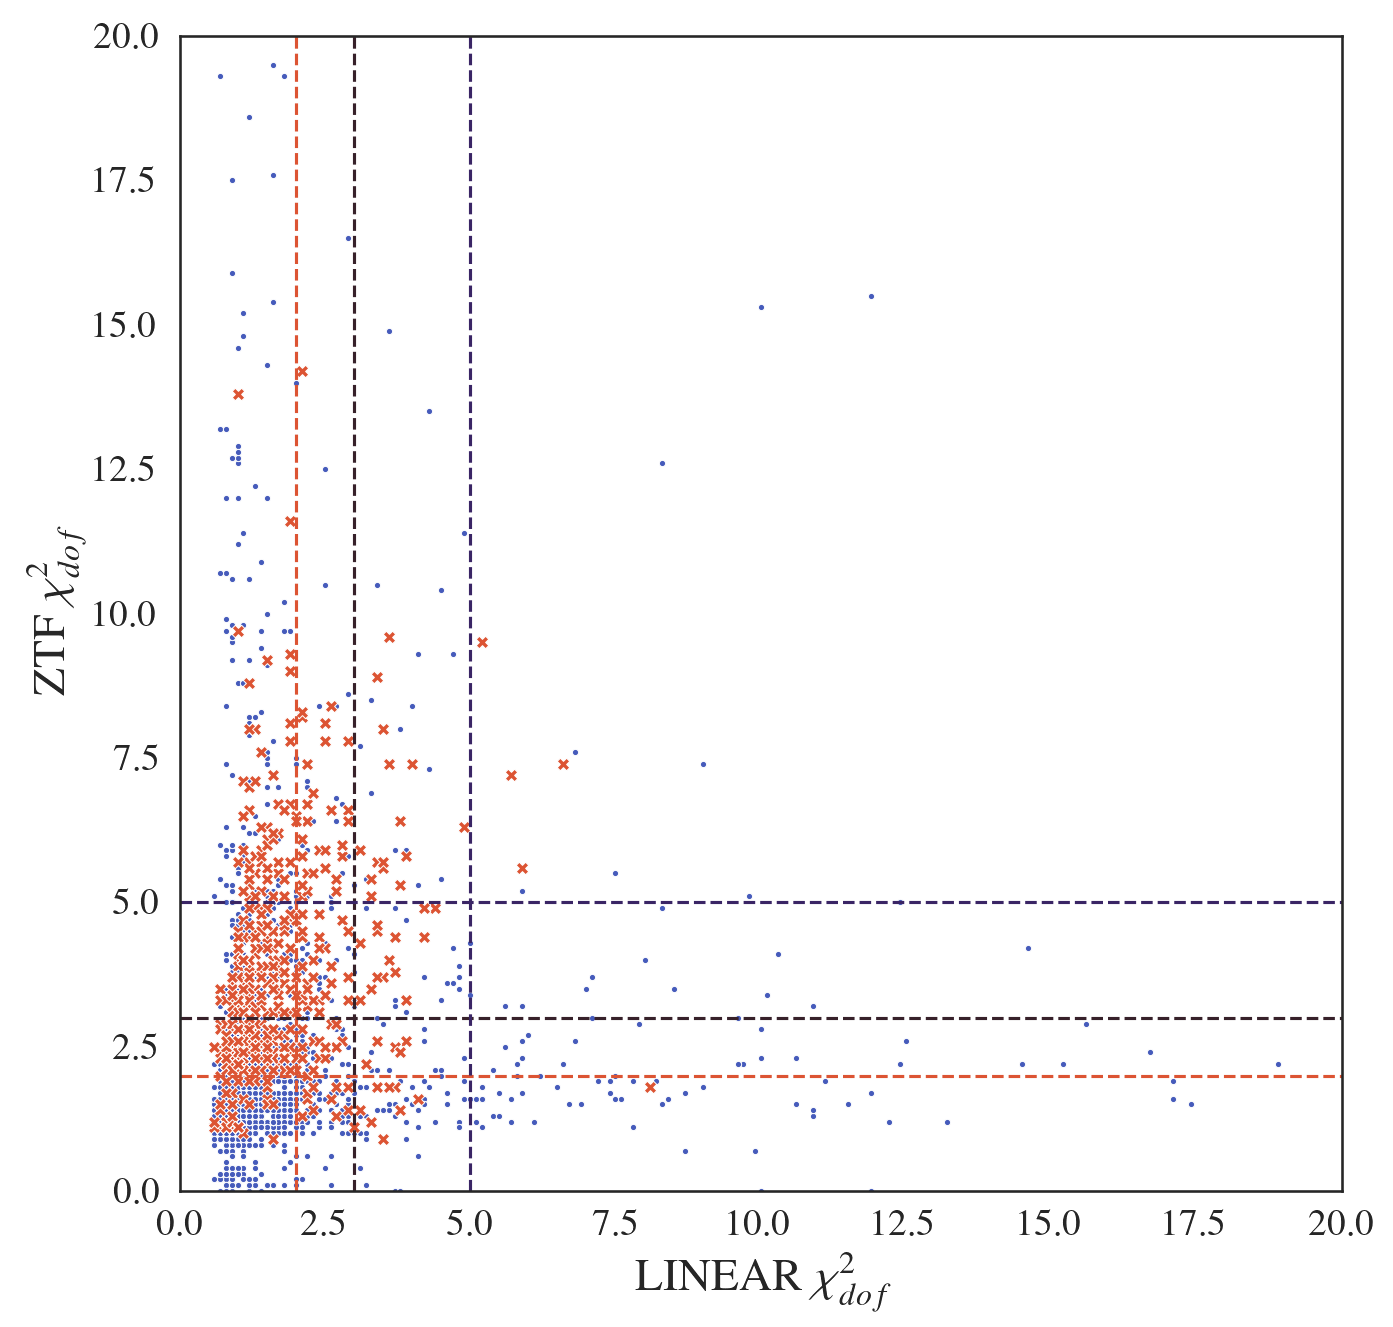
\includegraphics[width=17cm]{candidate_chi2_overlap.png}}
\caption{A selection diagram constructed with the two sets of robust $\chi^2_{dof}$ values, for LINEAR and ZTF data sets, where
  blue symbols represents all RR Lyrae stars, light red symbols represent all the Blazhko candidate stars, and the dark red symbols are the final sample of Blazhko stars. The horizontal
  and vertical dashed lines mark Blazhko candidate selection boundaries (see text).}
\label{fig:chi2}
\end{figure}


Given the two sets of light curves from LINEAR and ZTF, we searched for amplitude and phase modulation,
either during the 5-6 years of data taking by each survey, or during the average span of 15 years between the two
surveys. Starting with a sample of 2857 RR Lyrae stars, we pre-selected a smaller sample that was inspected
visually (see below for details). We also required at least 150 LINEAR data points and 150 ZTF data points (for the selected band from which we calculated the period)
in analyzed light curves. We used two pre-selection methods that are sensitive to different types of light curve
modulation: direct light curve analysis and periodogram analysis, as follows.
 

 
\subsection{Direct Light Curve Analysis}

\begin{figure*}[ht]
    \centering
    \resizebox{\hsize}{!}{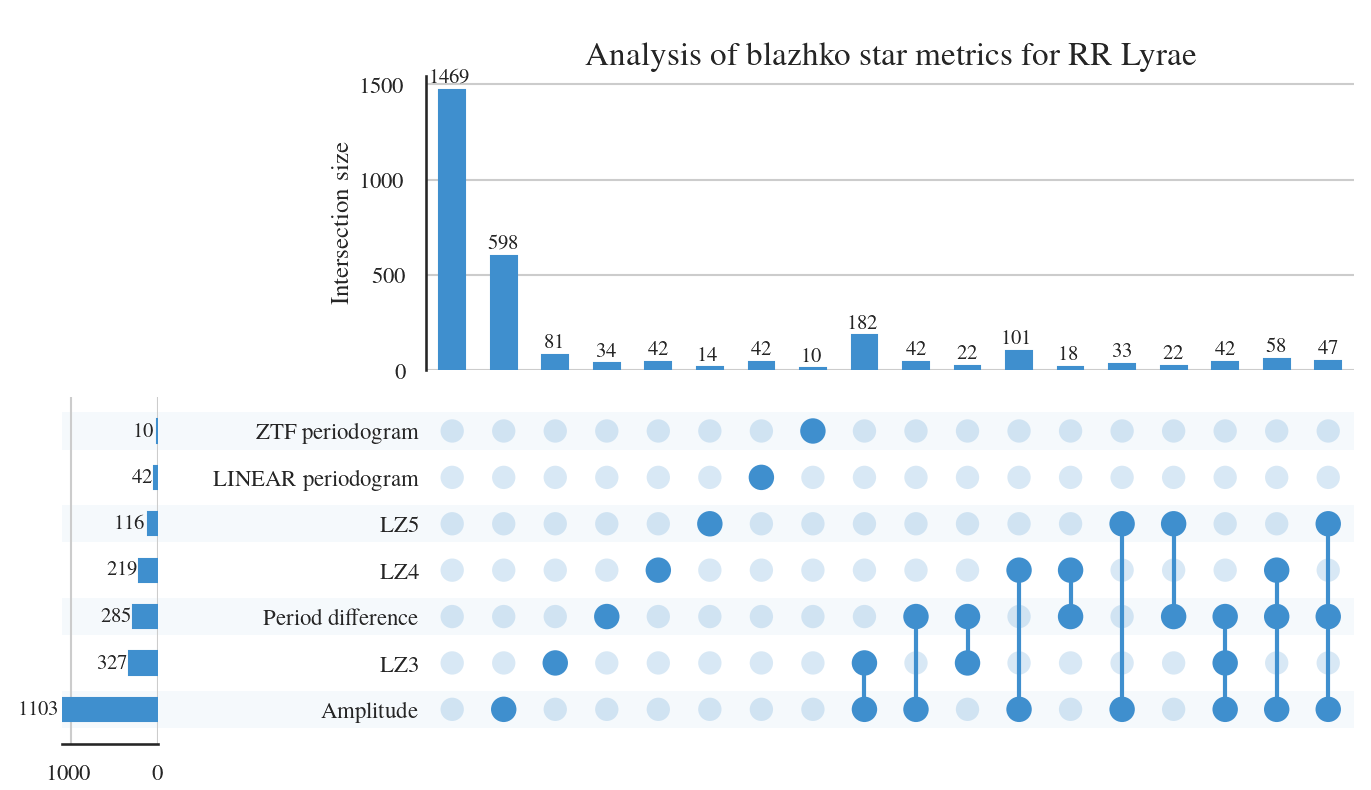
\includegraphics[width=21cm]{candidate_metrics.png}}
    \vskip -0.1in
    \caption{The figure shows selection criteria and the resulting numbers of pre-selected Blazhko star candidates for each
      criterion and their combinations. The dots represent each case a star can occupy, where every solid dot is a specific
      criterion that is satisfied. Connections between solid dots represent stars which satisfy multiple criteria. Each dot
      combination has its own count, represented by the horizontal countplot. The vertical countplot shows the total number
      of stars that satisfy one criteria (union of all cases).}
      \label{fig:selstats}
    \end{figure*}
    
Given statistically correct period, amplitude and light curve shape estimates,
as well as data being consistent with reported (presumably Gaussian) uncertainty estimates, the $\chi^2$ per degree
of freedom gives a quantitative assessment of the \textit{"goodness of fit"},
\begin{equation}
        \chi_{dof}^2 = {1 \over N_{dof}} \, \sum{\frac{(d_i - m_i)^2}{\sigma_i^2}}.
\end{equation}
Here, $d_i$ are measured light curve data values at times $t_i$, and with associated uncertainties $\sigma_i$,
$m_i$ are best-fit models at times $t_i$, and $N_{dof}$ is the number of degrees of freedom, essentially the
number of data points. In the absence of any light curve modulation, the expected value of $\chi^2_{dof}$ is
unity, with a standard deviation of $\sqrt(2/N_{dof}$.  If $\chi^2_{dof} - 1$ is many times  larger than 
$\sqrt(2/N_{dof}$, it is unlikely that data $d_i$ were generated by the assumed (unchanging) model $m_i$.  
Of course, $\chi^2_{dof}$ can also be large due to underestimated measurement uncertainties $\sigma_i$,
or to occasional non-Gaussian measurement error (the so-called outliers). 

Therefore, to search for signatures of the Blazhko effect, manifested through statistically unlikely large values
of $\chi^2_{dof}$, we computed $\chi^2_{dof}$ separately for LINEAR and ZTF data (see Figure~\ref{fig:chi2}). 
Using the two sets of $\chi^2_{dof}$ values, we algorithmically pre-selected a sample of candidate Blazhko stars
for further visual analysis of their light curves. The visual analysis is needed to confirm the expected Blazhko behavior
in observed light curves, as well as to identify cases of data problems, such as photometric outliers. 

We used a simple scoring algorithm, optimized through trial and error, illustrated in Fig.~\ref{fig:chi2} with dashed lines signifying $\chi^2_{dof}$ boundaries.
The algorithm used area boundaries for $\chi^2_{dof}$ values ($\chi^2_L$ is the $\chi^2_{dof}$ value for LINEAR, while $\chi^2_Z$ is analogous for ZTF data.)

The \textit{3-point area} includes ranges of:
\begin{enumerate}
    \item $\chi^2_L > 2.0$ and $\chi^2_L < 3.0$ and $\chi^2_Z > 2.0$ and $\chi^2_Z < 3.0$,
    \item $\chi^2_L > 2.0$ and $\chi^2_L < 3.0$ and $\chi^2_Z < 3.0$,
    \item $\chi^2_Z > 2.0$ and $\chi^2_Z < 3.0$ and $\chi^2_L <3.0$.
\end{enumerate}

The \textit{4-point area} includes ranges of:

\begin{enumerate}
\item $\chi^2_L > 3.0$ and $\chi^2_L < 5.0$ and $\chi^2_Z < 3.0$
\item $\chi^2_L < 3.0$ and $\chi^2_Z > 3.0$ and $\chi^2_Z < 5.0$
\end{enumerate}
    
The \textit{5-point area} includes ranges of:

\begin{enumerate}
\item $\chi^2_L > 5.0$ and $\chi^2_Z > 5.0$
\item $\chi^2_L > 3.0$ and $\chi^2_L < 5.0$ and $\chi^2_Z > 3.0$ and $\chi^2_Z < 5.0$
\item $\chi^2_L > 5.0$ and $\chi^2_Z < 5.0$
\item $\chi^2_Z > 5.0$ and $\chi^2_L < 5.0$
\end{enumerate}

In addition, we also considered normalized period differences ($dP$) and amplitude differences ($dA$) and assigned: 1 points for $0.00002 < dP < 0.00005$
and 2 points for $dP > 0.00005$; 1 point for $0.05 < dA < 0.15$ and 2 points for $dA > 0.15$. 
A star could score a maximum of 9 points, and a minimum of 5 points was required for further visual analysis. 

The sample pre-selected using this method includes 531 stars. For most selected stars, the $\chi^2_{dof}$ values were
larger for the ZTF data because the ZTF photometric uncertainties are smaller than for the LINEAR data set. 
Fig.~\ref{fig:selstats} summarizes the selection criteria and the resulting numbers of selected stars for each
criterion and their combinations. 
 


\subsection{Periodogram Analysis} 


\begin{figure*}[ht]
  \centering
  \resizebox{\hsize}{!}{\includegraphics[width=14cm]{periodogram.png}}
  \caption{The top two panels show a simulated periodogram for a sum of two {\it sine} functions with similar frequencies
    $f_1$ and  $f_2$ --   the central peak corresponds to their mean (see eqs.~\ref{eq:fo} and \ref{eq:Df}).
    The bottom left panel shows a periodogram for an observed LINEAR light curve, and the bottom right panel shows its
    folded version (around the main frequency $f_o=1.585$ d$^{-1}$). In the bottom left panel, the three vertical dashed
    lines show the three  frequencies identified by the algorithm described in text, and the two dot-dashed lines mark
    yearly aliases around the main frequency $f_o$, at frequencies $f_o \pm 0.00274$ d$^{-1}$. The two vertical lines in the
    bottom right panel have the same meaning, and the horizontal dashed line shows the noise level multiplied by 5.}
\label{fig:periodogram}
\end{figure*}

  
When light curve modulation is due to double-mode oscillation with two similar oscillation frequencies (periods),
it is possible to recognize its signature in the periodogram computed as part of the Lomb-Scargle analysis. Depending
on various details, such as data sampling and the exact values of periods, amplitudes, this method may be
more efficient than direct light curve analysis \citep{2020MNRAS.494.1237S}. 

A sum of two {\it sine} functions with same amplitudes and with frequencies $f_1$ and $f_2$ can be rewritten 
using trigonometric equalities as 
\begin{equation}
         y(t) = 2 \, \cos(2\pi{f_1-f_2\over 2} t) \, \sin(2\pi {f_1+f_2\over 2} t).
\end{equation} 
We can define 
\begin{equation}
\label{eq:fo}
         f_o = {f_1+f_2\over 2},
\end{equation} 
and 
\begin{equation}
\label{eq:Df}
         \Delta f = |{f_1-f_2\over 2}|,
\end{equation} 
with $\Delta f << f_o$ when $f_1$ and $f_2$ are similar. The fact that $\Delta f$ is much smaller than $f_o$ means
that the period of the {\it cos} term
is much larger than the period of the basic oscillation ($f_o$). In other words, the {\it cos} term acts as a slow
amplitude modulation of the basic oscillation. When the amplitudes of two {\it sine} functions are not equal, the
results are more complicated but the basic conclusion about amplitude modulation remains.
When the power spectrum of $y(t)$ is constructed, it will show 3 peaks: the main peak at $f_o$ and
two more peaks at frequencies $f_o \pm \Delta f$. We used this fact to construct an algorithm for
automated searching for the evidence of amplitude  modulation. 
Fig \ref{fig:periodogram} compares the theoretical periodogram produced by interference beats with our algorithm's periodogram,
signifying that local Blazhko peaks are present in real data.

\begin{figure}[ht]
  \resizebox{\hsize}{!}{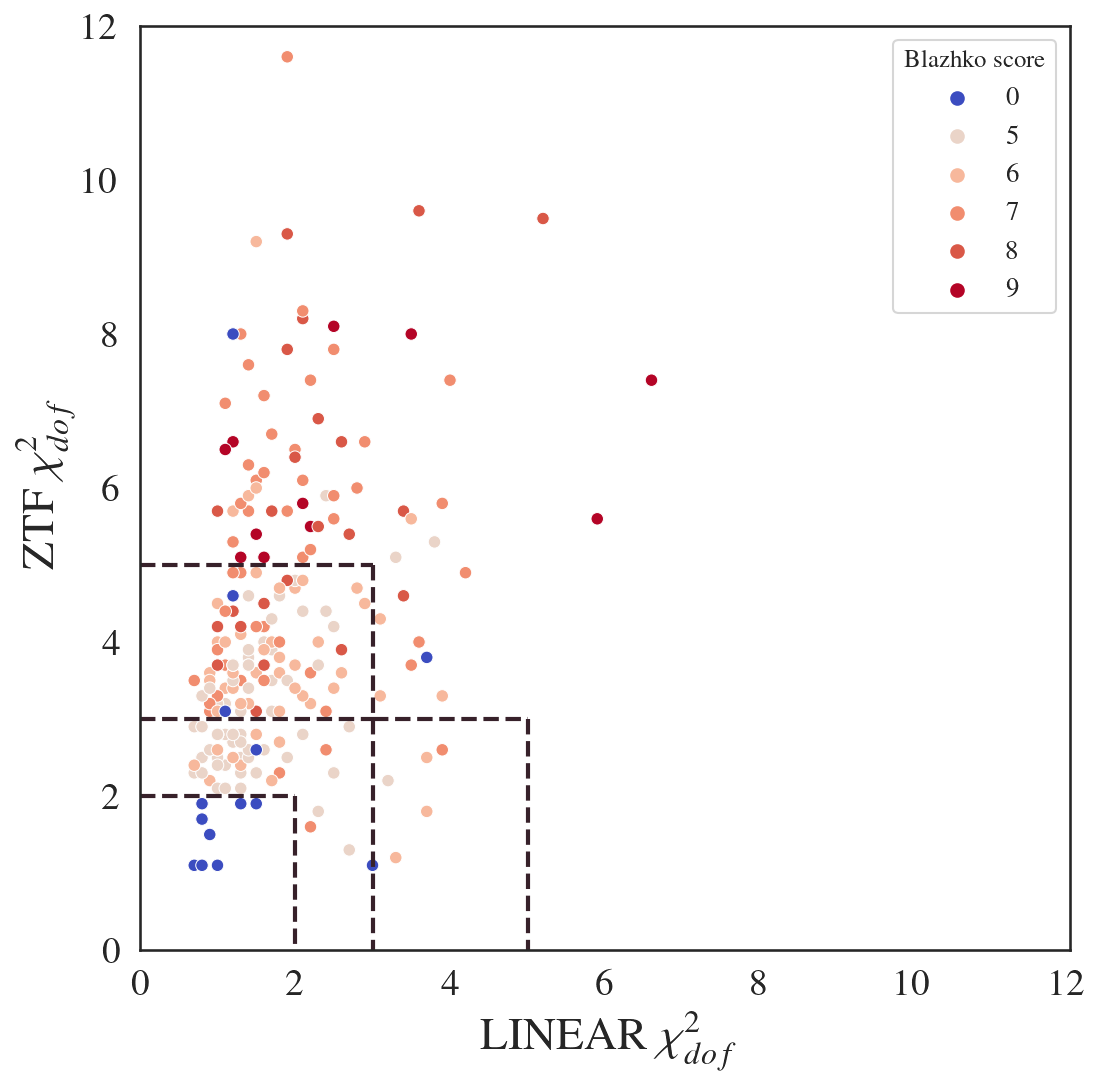
\includegraphics[width=17cm]{final_chi2_b.png}}
  \caption{The figure shows in which $\chi^2_{dof}$ area Blazhko stars are. Each dot is colored a different shade of red
  based on its score during selection, while blue dots are stars selected via periodogram.}
  \label{fig:chi_final}
  \end{figure}

After the strongest peak in the Lomb-Scargle periodogram is found at frequency $f_o$, we search for  two equally
distant local peaks at frequencies $f_-$ and $f_+$, with $f_- < f_0 < f_+$.  The sideband peaks can be highly asymmetric
\cite{2003ApJ...598..597A} and observed periodograms can sometimes be much more complex \cite{2007MNRAS.377.1263S}.  
We fold the periodogram through the main peak at $f_o$, multiply the two branches and then search for the strongest peaks
in the resulting folded periodogram that is statistically more significant than the background noise. The background noise
is computed as the scatter of the folded periodogram estimated from the interquartile range. We require a ``signal-to-noise''
ratio of at least 5, as well as the peak strength of at least 0.05 for ZTF, while 0.10 for LINEAR data. 
If such a peak is found,
and it doesn't correspond to yearly alias, we select the star as a candidate Blazhko star and compute
its Blazhko period as 
\begin{equation*}
P_{BL} = |f_{-,+} - f_0|^{-1},
\end{equation*}
where $f_{-,+}$ means the Blazhko sideband frequency with a higher amplitude is chosen. 

The observed Blazhko periods range from 3 to 3,000 days, and Blazhko amplitudes range from 0.01 mag to about 0.3 mag \citep{2007MNRAS.377.1263S}. In this work, we selected a smaller Blazhko range due to the limitations of our data: 30--325 days. 
With this additional constraint, we selected 52 candidate Blazhko stars. 
Fig \ref{fig:periodogram} shows an example where two very prominent peaks were identified in the LINEAR periodogram. 



\subsubsection{Visual Confirmation}

\begin{figure*}[ht]
  \centering
%  
\includegraphics[width=17cm]{LCplot_7048826.png}
  \resizebox{\hsize}{!}{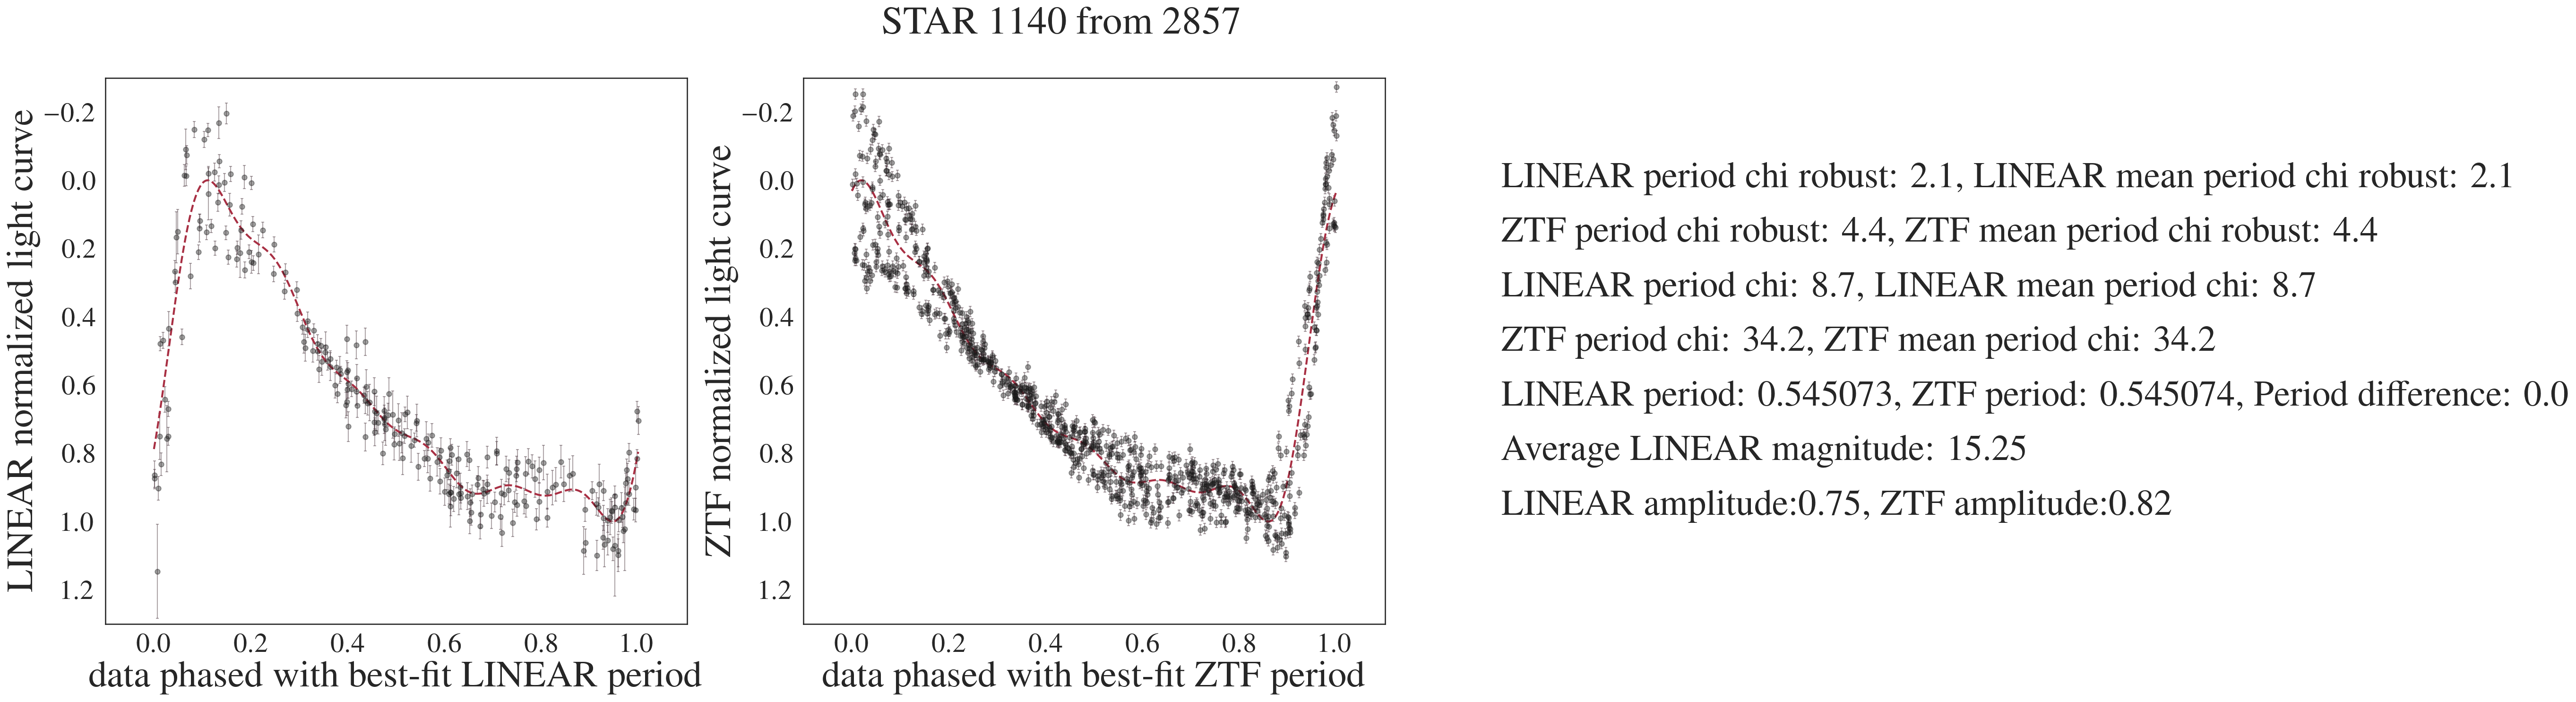
\includegraphics[width=17cm]{LCplot_10030349.png}}
  \caption{An illustration of visual analysis of phased light curves for the selected Blazhko candidates. The left
    panel shows LINEAR data and the right panel shows ZTF data
    (symbols with ``error bars'') for star with LINEARid = 1212611. The dashed
    lines are best-fit models. The numbers listed on the right side were added to aid  visual analysis. Note
    multiple coherent data point sequences offset from the best-fit mean model in the right panel.}
       \label{fig:phase1}
\end{figure*}

\begin{figure*}[ht] 
    \centering
%        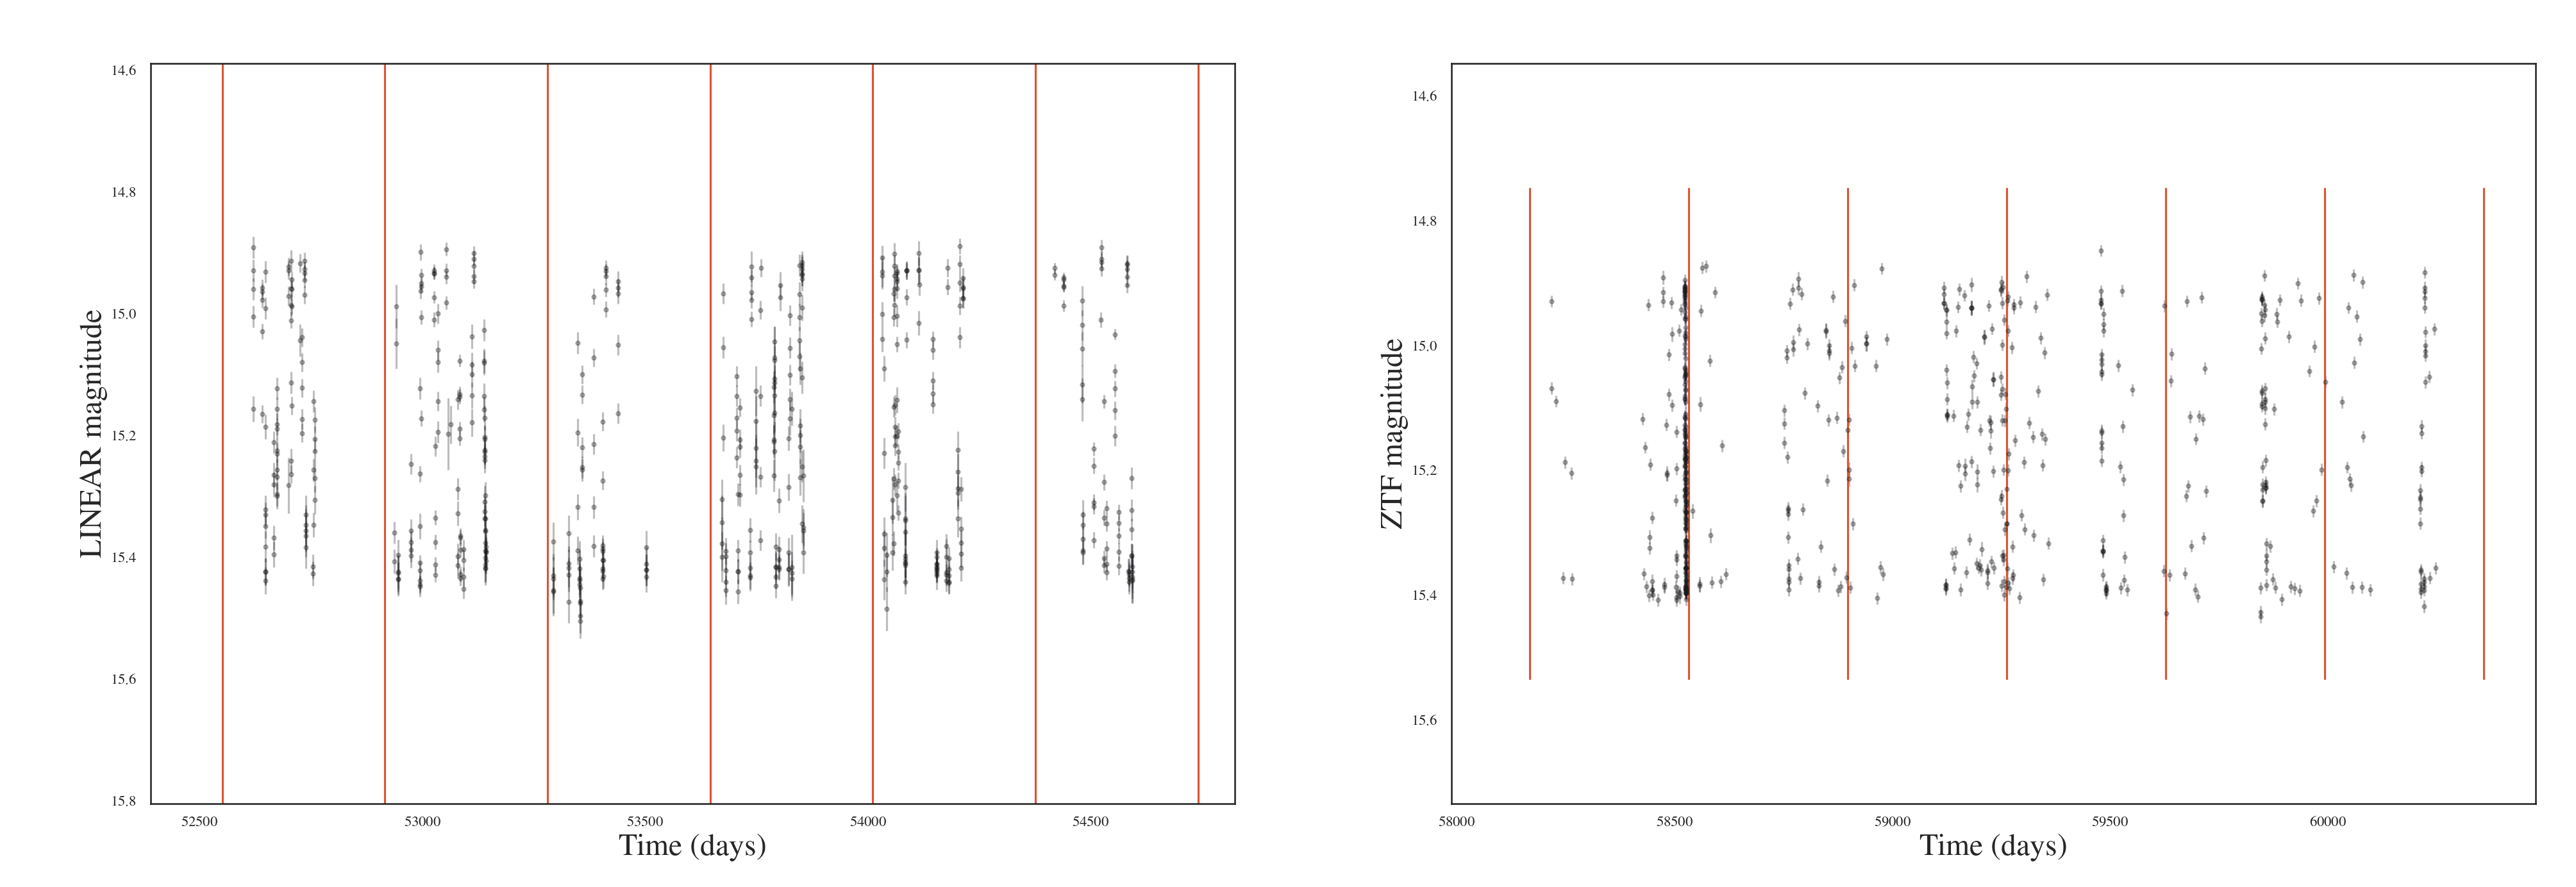
\includegraphics[width=17cm]{season_plot7048826.png}
      \resizebox{\hsize}{!}{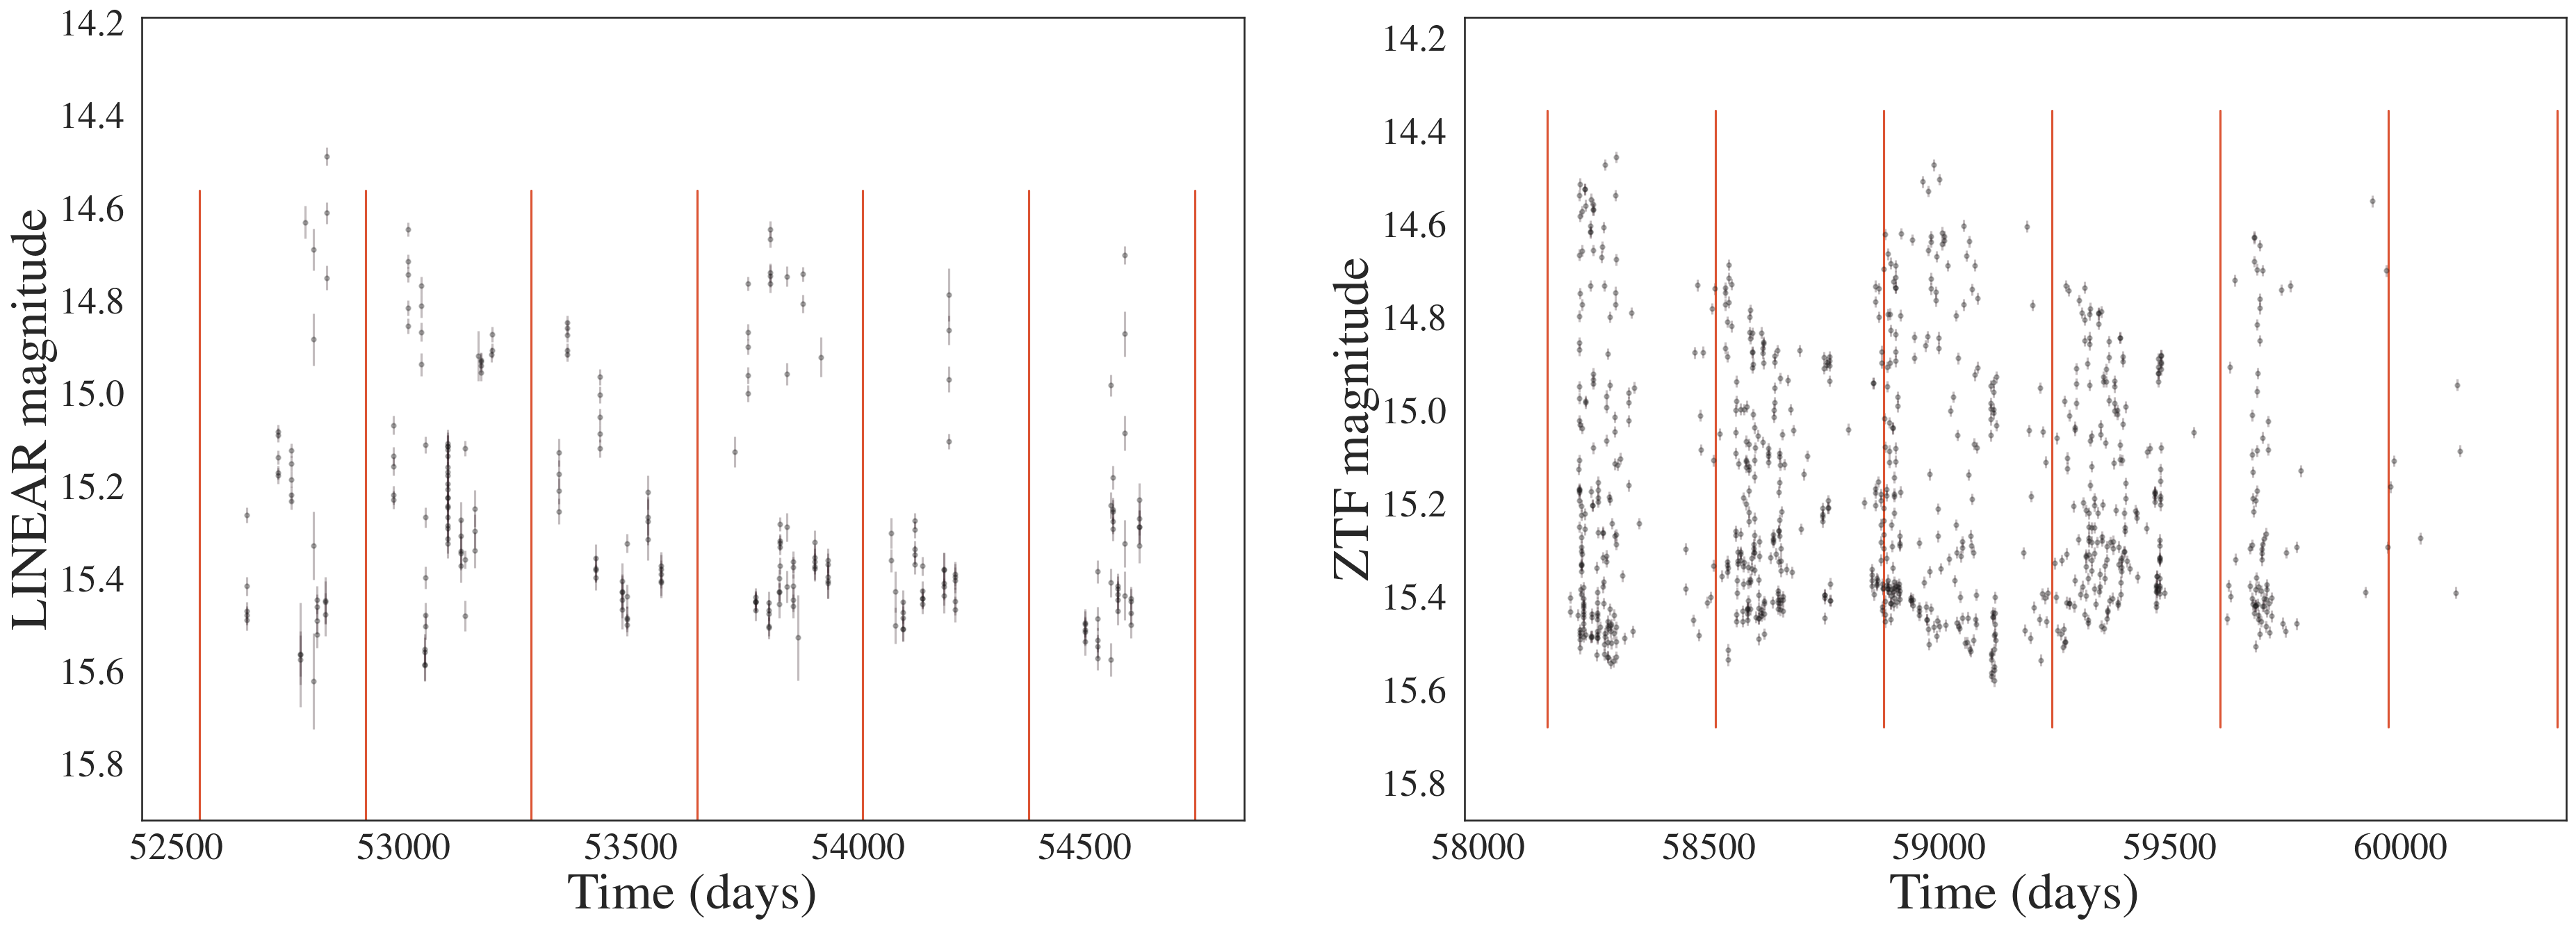
\includegraphics[width=17cm]{season_plot10030349.png}}
       \caption{An illustration of visual analysis of full light curves for the selected Blazhko candidates with emphasis
         on their repeatability between observing seasons, marked with  vertical lines (left: LINEAR data; right: ZTF data). Data
         shown are for star with LINEARid = 1212611. }
         \label{fig:phase3}
\end{figure*}
       
\begin{figure*}[ht]
    \centering
%    \includegraphics[width=17cm]{LCplotBySeason7048826.png}
    \resizebox{\hsize}{!}{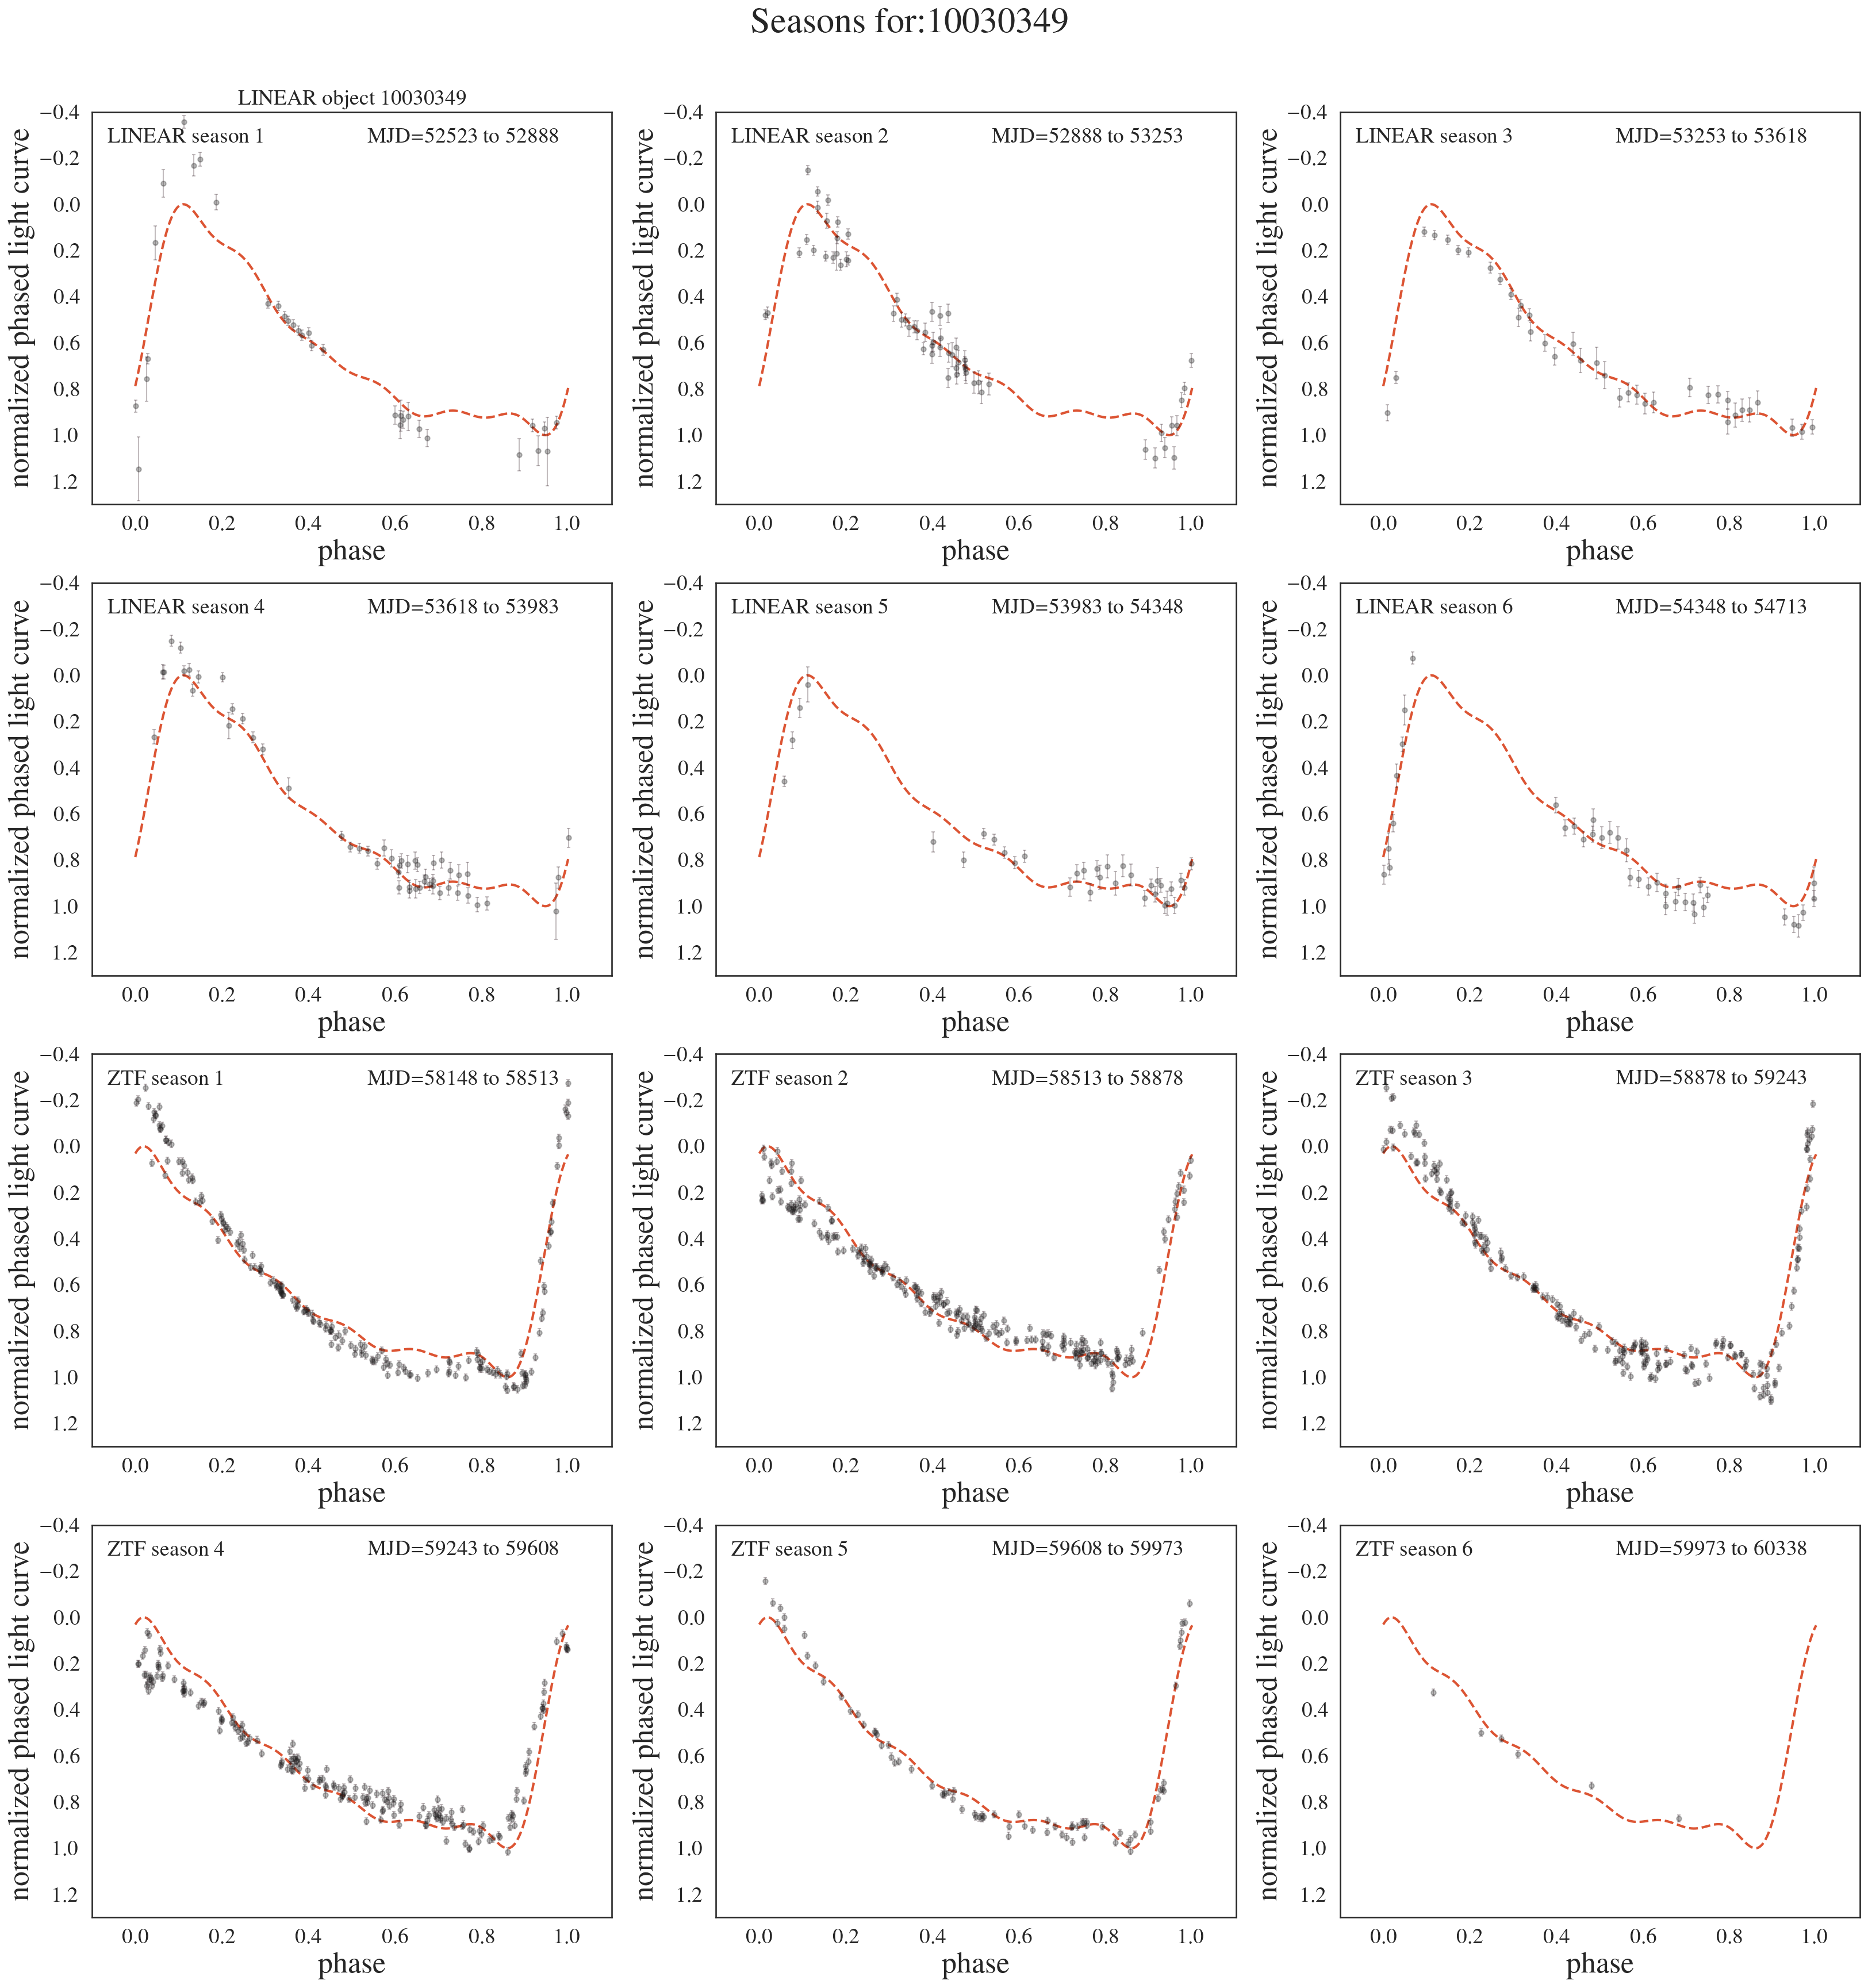
\includegraphics[width=16cm]{LCplotBySeason10030349.png}}
    \caption{The phased light curves normalized to unit amplitude are shown for single observing seasons
      and compared to the mean best-fit models (top six panels: LINEAR data; bottom six panels: ZTF data).
      Data shown are for star with LINEARid = 1212611.
      Season-to-season phase and amplitude modulations are seen in both the LINEAR and the ZTF data.}
      \label{fig:phase4}
\end{figure*}



The sample pre-selected for visual analysis includes 531 RR Lyrae stars (479 + 52),
or 18.1\% of the starting LINEAR-ZTF sample. Visual analysis included the following standard steps
\citep[e.g.,][]{2009MNRAS.400.1006J, 2017MNRAS.466.2602P}: 
\begin{enumerate}
\item The shape of the phased light curves and scatter of data points around the best-fit model were examined
    for signatures of anomalous behavior indicative of the Blazhko effect. 
    Fig.~\ref{fig:phase1} shows an example of such behavior where the ZTF data and fit show multiple coherent data point sequences
    offset from the best-fit mean model. 
  \item Full light curves were inspected for their repeatability between observing seasons (Fig.~\ref{fig:phase3}).
       This step was sensitive to amplitude modulations with periods of the order a year or longer.  
     \item The phased light curves normalized to unit amplitude were inspected for their repeatability between observing seasons.
       This step was sensitive to phase modulations of a few percent or larger on time scales of the order a year or longer.  
       Fig.~\ref{fig:phase4} shows an example of a Blazhko star where season-to-season phase (and amplitude) modulations
       are seen in both the LINEAR data and (especially) the ZTF data. 
\end{enumerate}

After visually analyzing the starting sample of 531 Blazhko candidates, we visually confirmed expected Blazhko
behavior for 228 stars (214 out of 479 and 14 out of 52). LINEAR IDs and other characteristics for confirmed
Blazhko stars are listed in Table 1 (Appendix A). Statistical properties of the selected sample of Blazhko stars are
discussed in detail in the next section. 




\section{Results}\label{sec:results}

Starting with a sample of 2857 field RR Lyrae stars with both LINEAR and ZTF data, we constructed a subsample of
1996 with light curves of sufficient quality and selected and verified 228 stars that exhibit convincing Blazhko effect.
In this section we compare various statistical properties of selected Blazhko stars to those of the starting sample. 

\subsection{The Blazhko Incidence Rate}

The implied incidence rate for the Blazhko effect is
11.4$\pm$0.8\%. Due to selection effects and unknown completeness,
this rate should be considered as a lower limit. 
When ab and c types are considered separately, the
rate is slightly higher for the former than for the latter: 12.1$\pm$0.9\%
vs. 9.2$\pm$1.3\%.  The difference of 2.9\% has low statistical significance ($<2\sigma$). 


\subsection{Period, Amplitude and Magnitude Distributions}

\begin{figure*}[ht]
    \centering
    \resizebox{\hsize}{!}{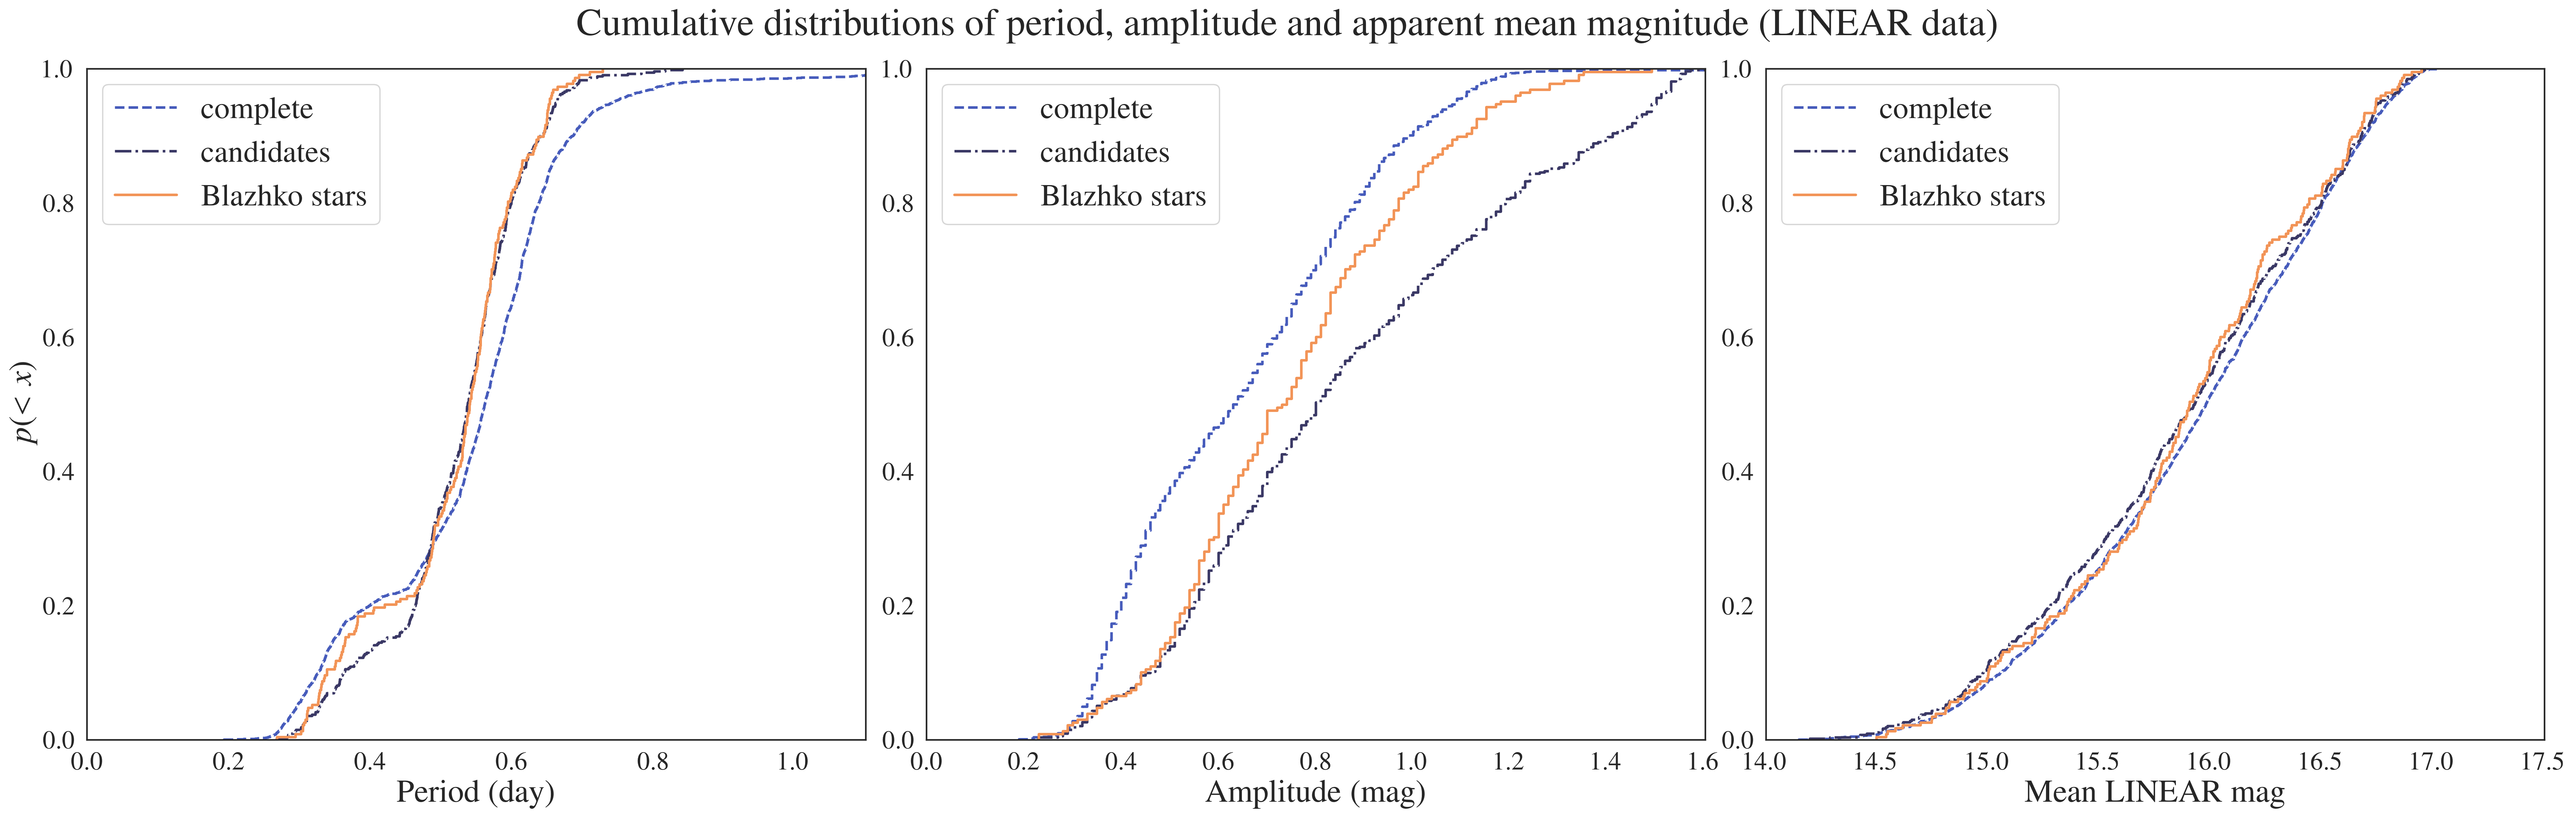
\includegraphics[width=16cm]{cumulative_distib_L.png}}
     \resizebox{\hsize}{!}{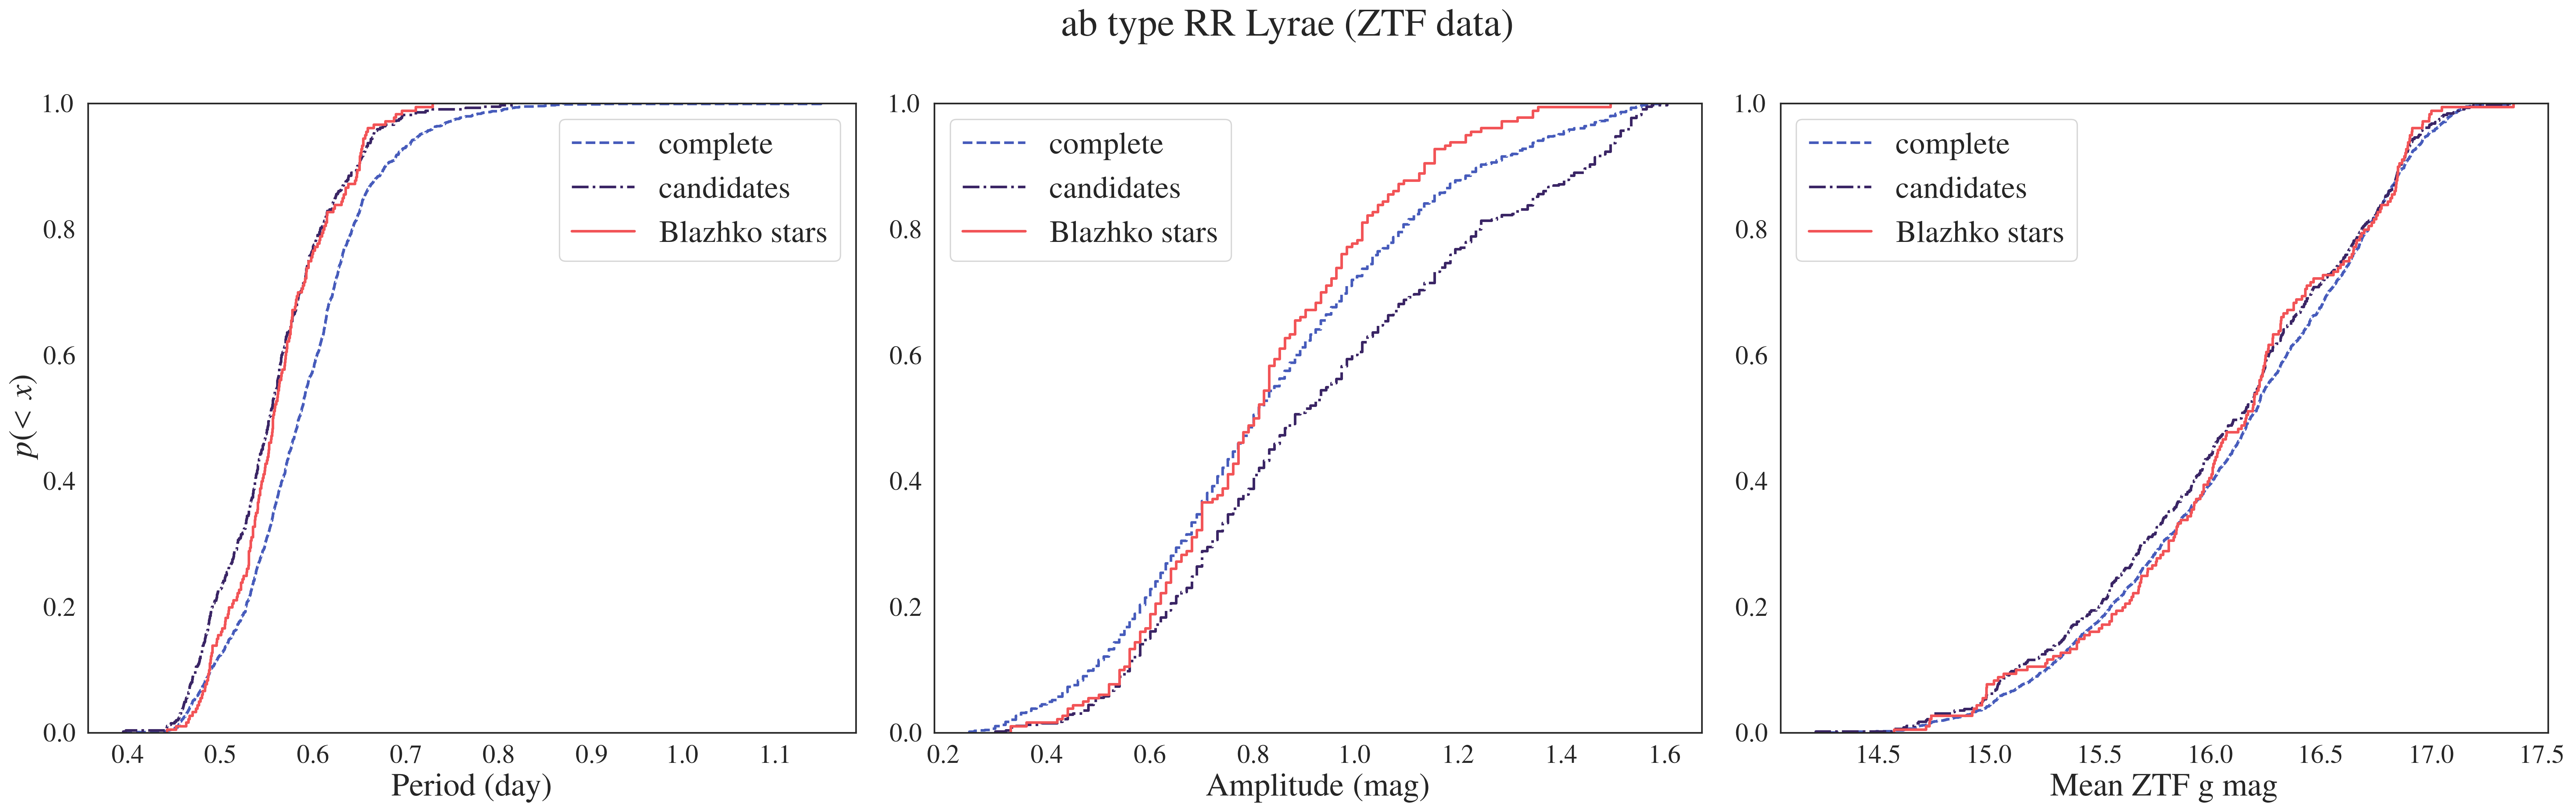
\includegraphics[width=16cm]{CDF_abtype.png}}
     \resizebox{\hsize}{!}{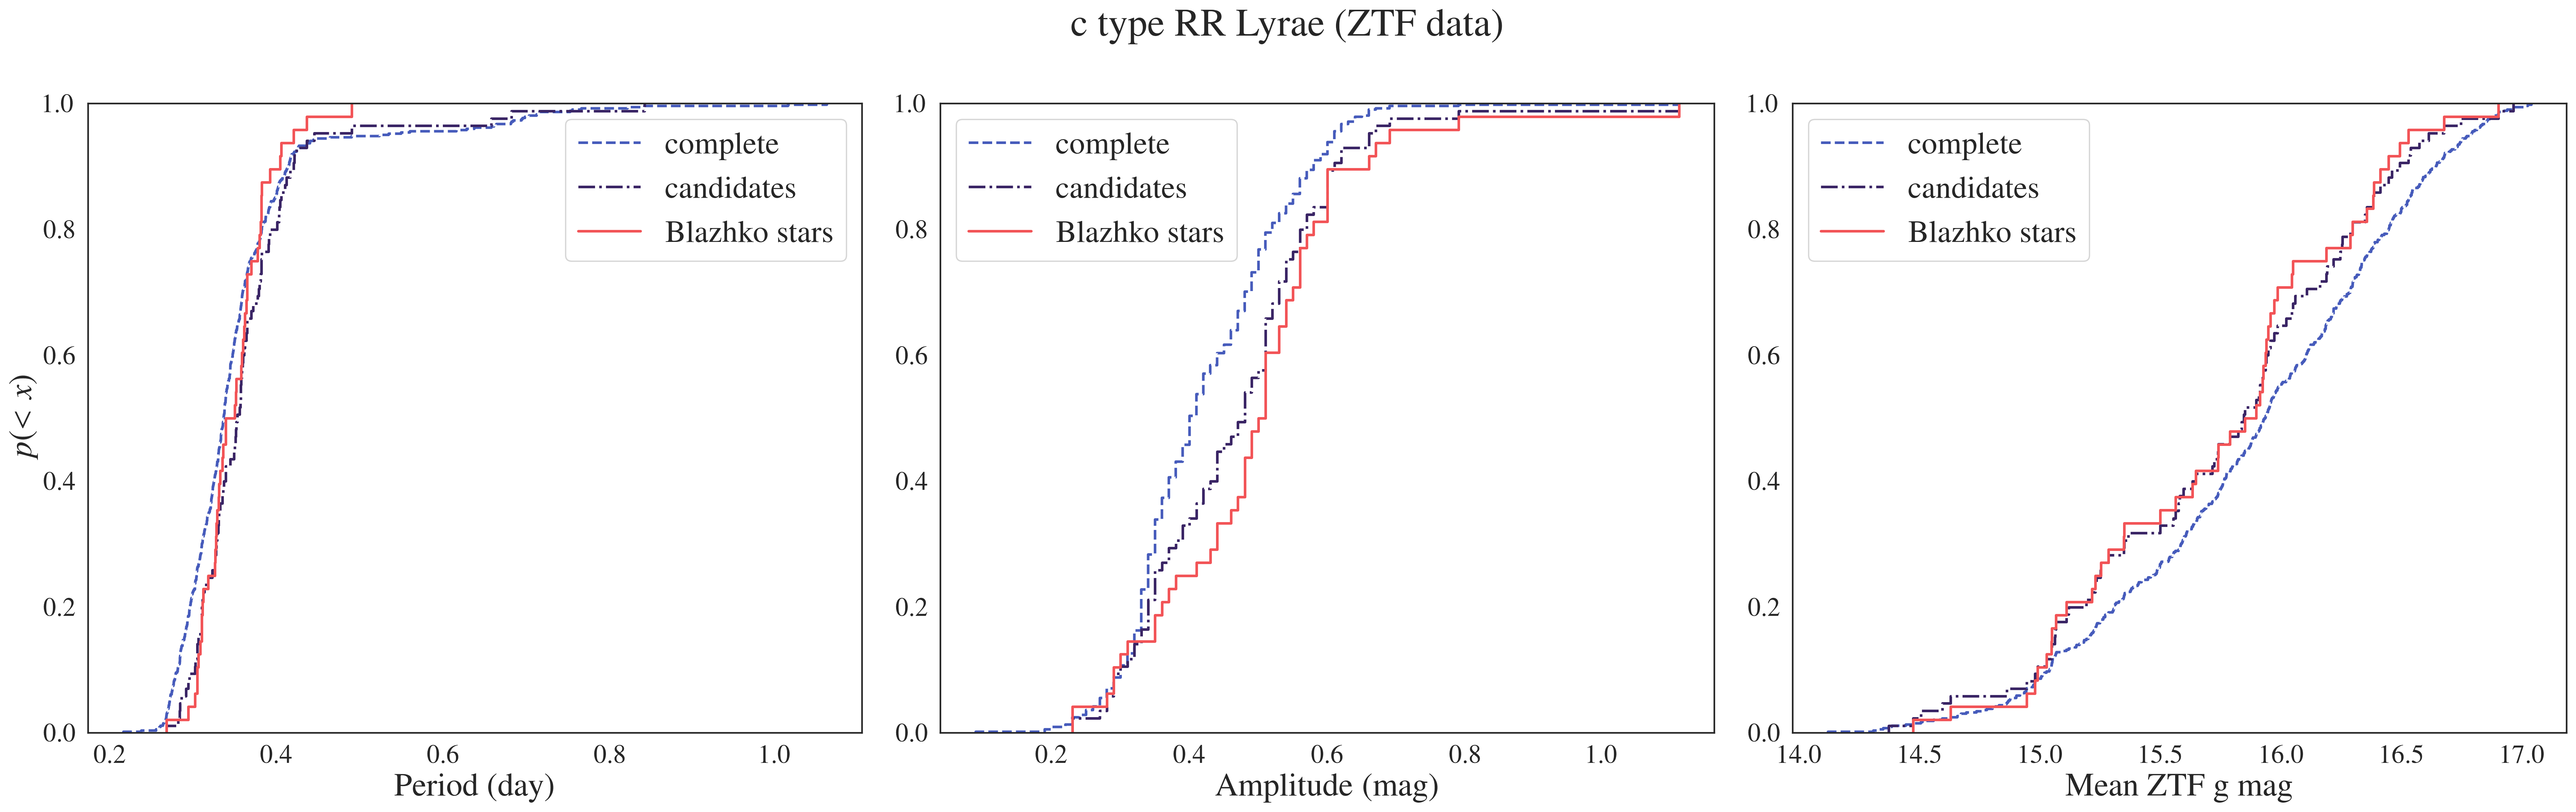
\includegraphics[width=16cm]{CDF_ctype.png}}
   \caption{A comparison of cumulative distributions of period (left),
   amplitude (middle) and apparent magnitude for starting sample,
   selected Blazhko candidates and visually verified Blazhko
   stars. The top row is based on LINEAR data and both ab type and c
   type stars. The middle and bottom rows are
   based on ZTF data, and show separately data for ab type and c type
   stars, respectively. The differences in period and amplitude
   distributions are futher examined in figure~\ref{fig:AmplPeriod2D}.}
      \label{fig:AmplPeriod}
\end{figure*}


\begin{figure*}[ht]
    \centering
    \resizebox{\hsize}{!}{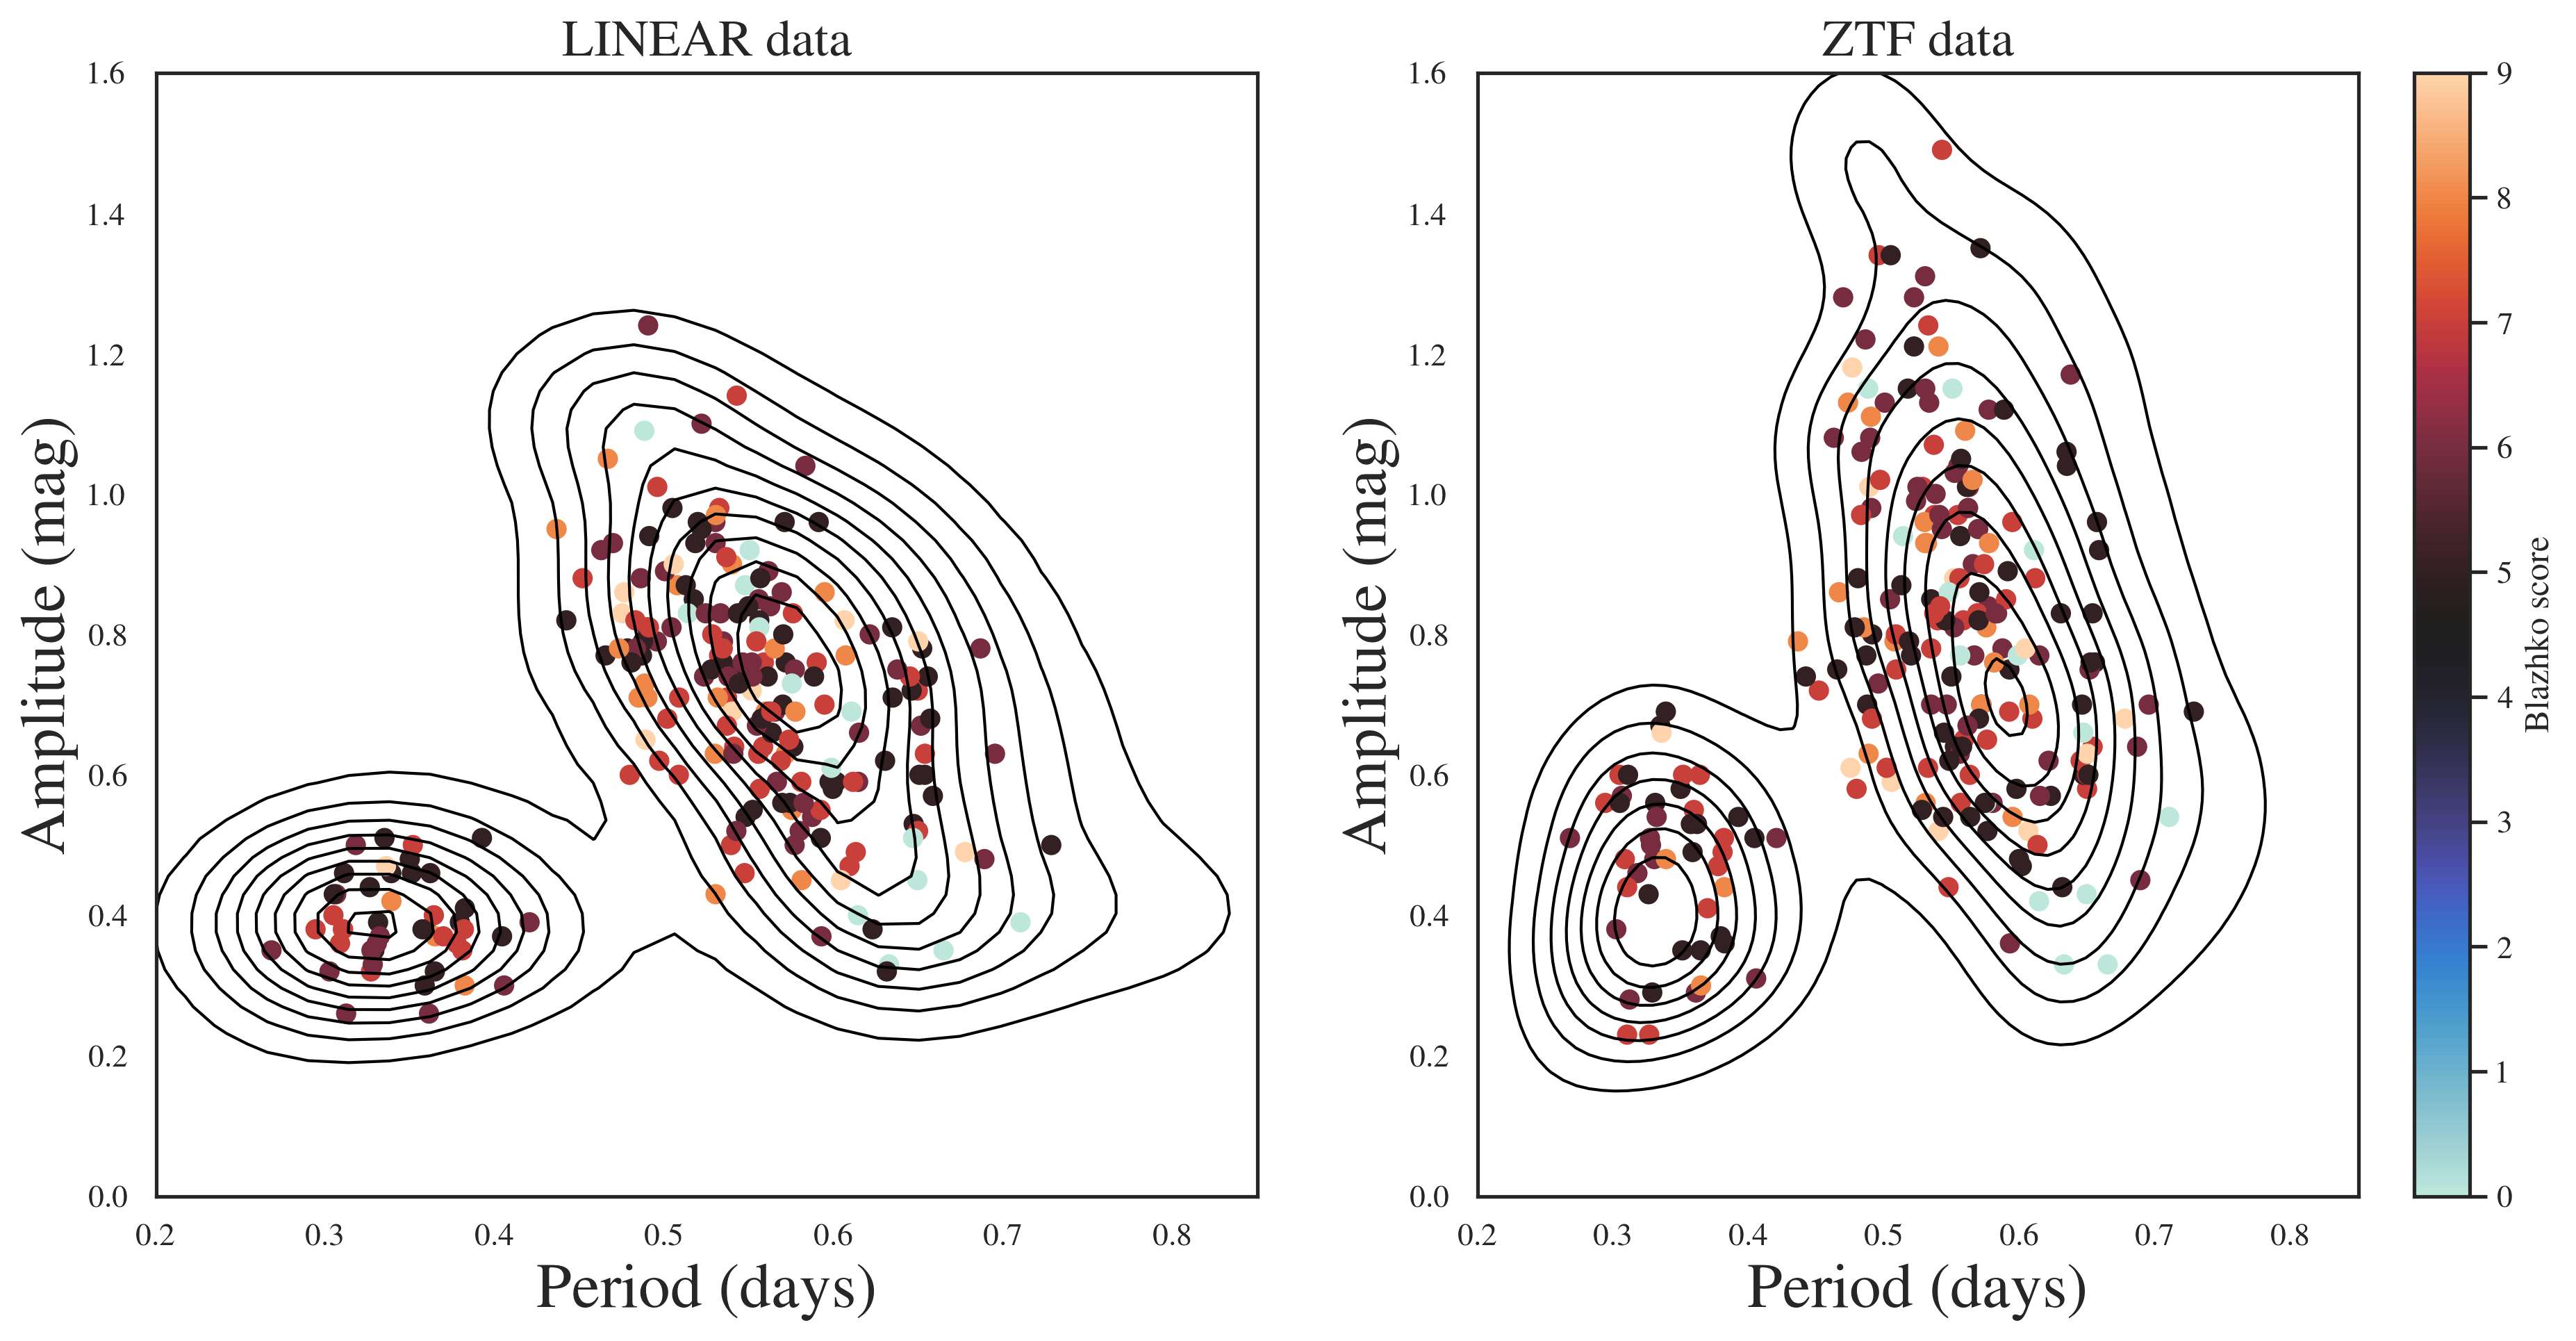
\includegraphics[width=16cm]{AmplPeriod.png}}
    \caption{Comparison of amplitude--period distributions (the Bailey
      diagram) for the starting sample of 1,996 RR Lyrae stars (contours)
        and 228 selected candidate Blazhko stars (symbols). The clump
        in the lower left corresponds to c type RR Lyrae and the
        other one to ab type. Note that the period distribution for ab
      type Blazhko stars is shifted left (by about 0.03 day, or 5\%).}
      \label{fig:AmplPeriod2D}
\end{figure*}

 
Marginal distributions of  period, amplitude and apparent magnitude
for the starting sample and Blazhko stars are compared in Fig.~\ref{fig:AmplPeriod}. 
Encouragingly, their magnitude distributions are statistically
indistinguishable which indicates that the completeness is not a
strong function of the photometric signal-to-noise ratio. This
result is probably due to the fact that the sample is defined by the
depth of LINEAR survey, while ZTF survey is deeper than this limit and
its photometric quality is approximately constant across the probed
magnitude range. 

The suspected differences in amplitude and period distributions are
further explored in Fig.~\ref{fig:AmplPeriod2D}. It is already
discernible by eye that the period distribution for Blazhko stars of
ab type is shifted to smaller values than for the starting sample. We have
found that the median period for ab type Blazhko stars is about 5\% shorter
than for the starting RR Lyrae sample. This difference is significant at
the 7.1$\sigma$ level.  At the same time, the difference in median
amplitudes for ab type stars corresponds to only 0.6$\sigma$ deviation. 
No statistically significant differences are found in period and
amplitude distributions for c type stars. 


\subsection{Long-term behavior of Blazhko Stars}

\begin{figure*}[ht]
    \centering
    \resizebox{\hsize}{!}{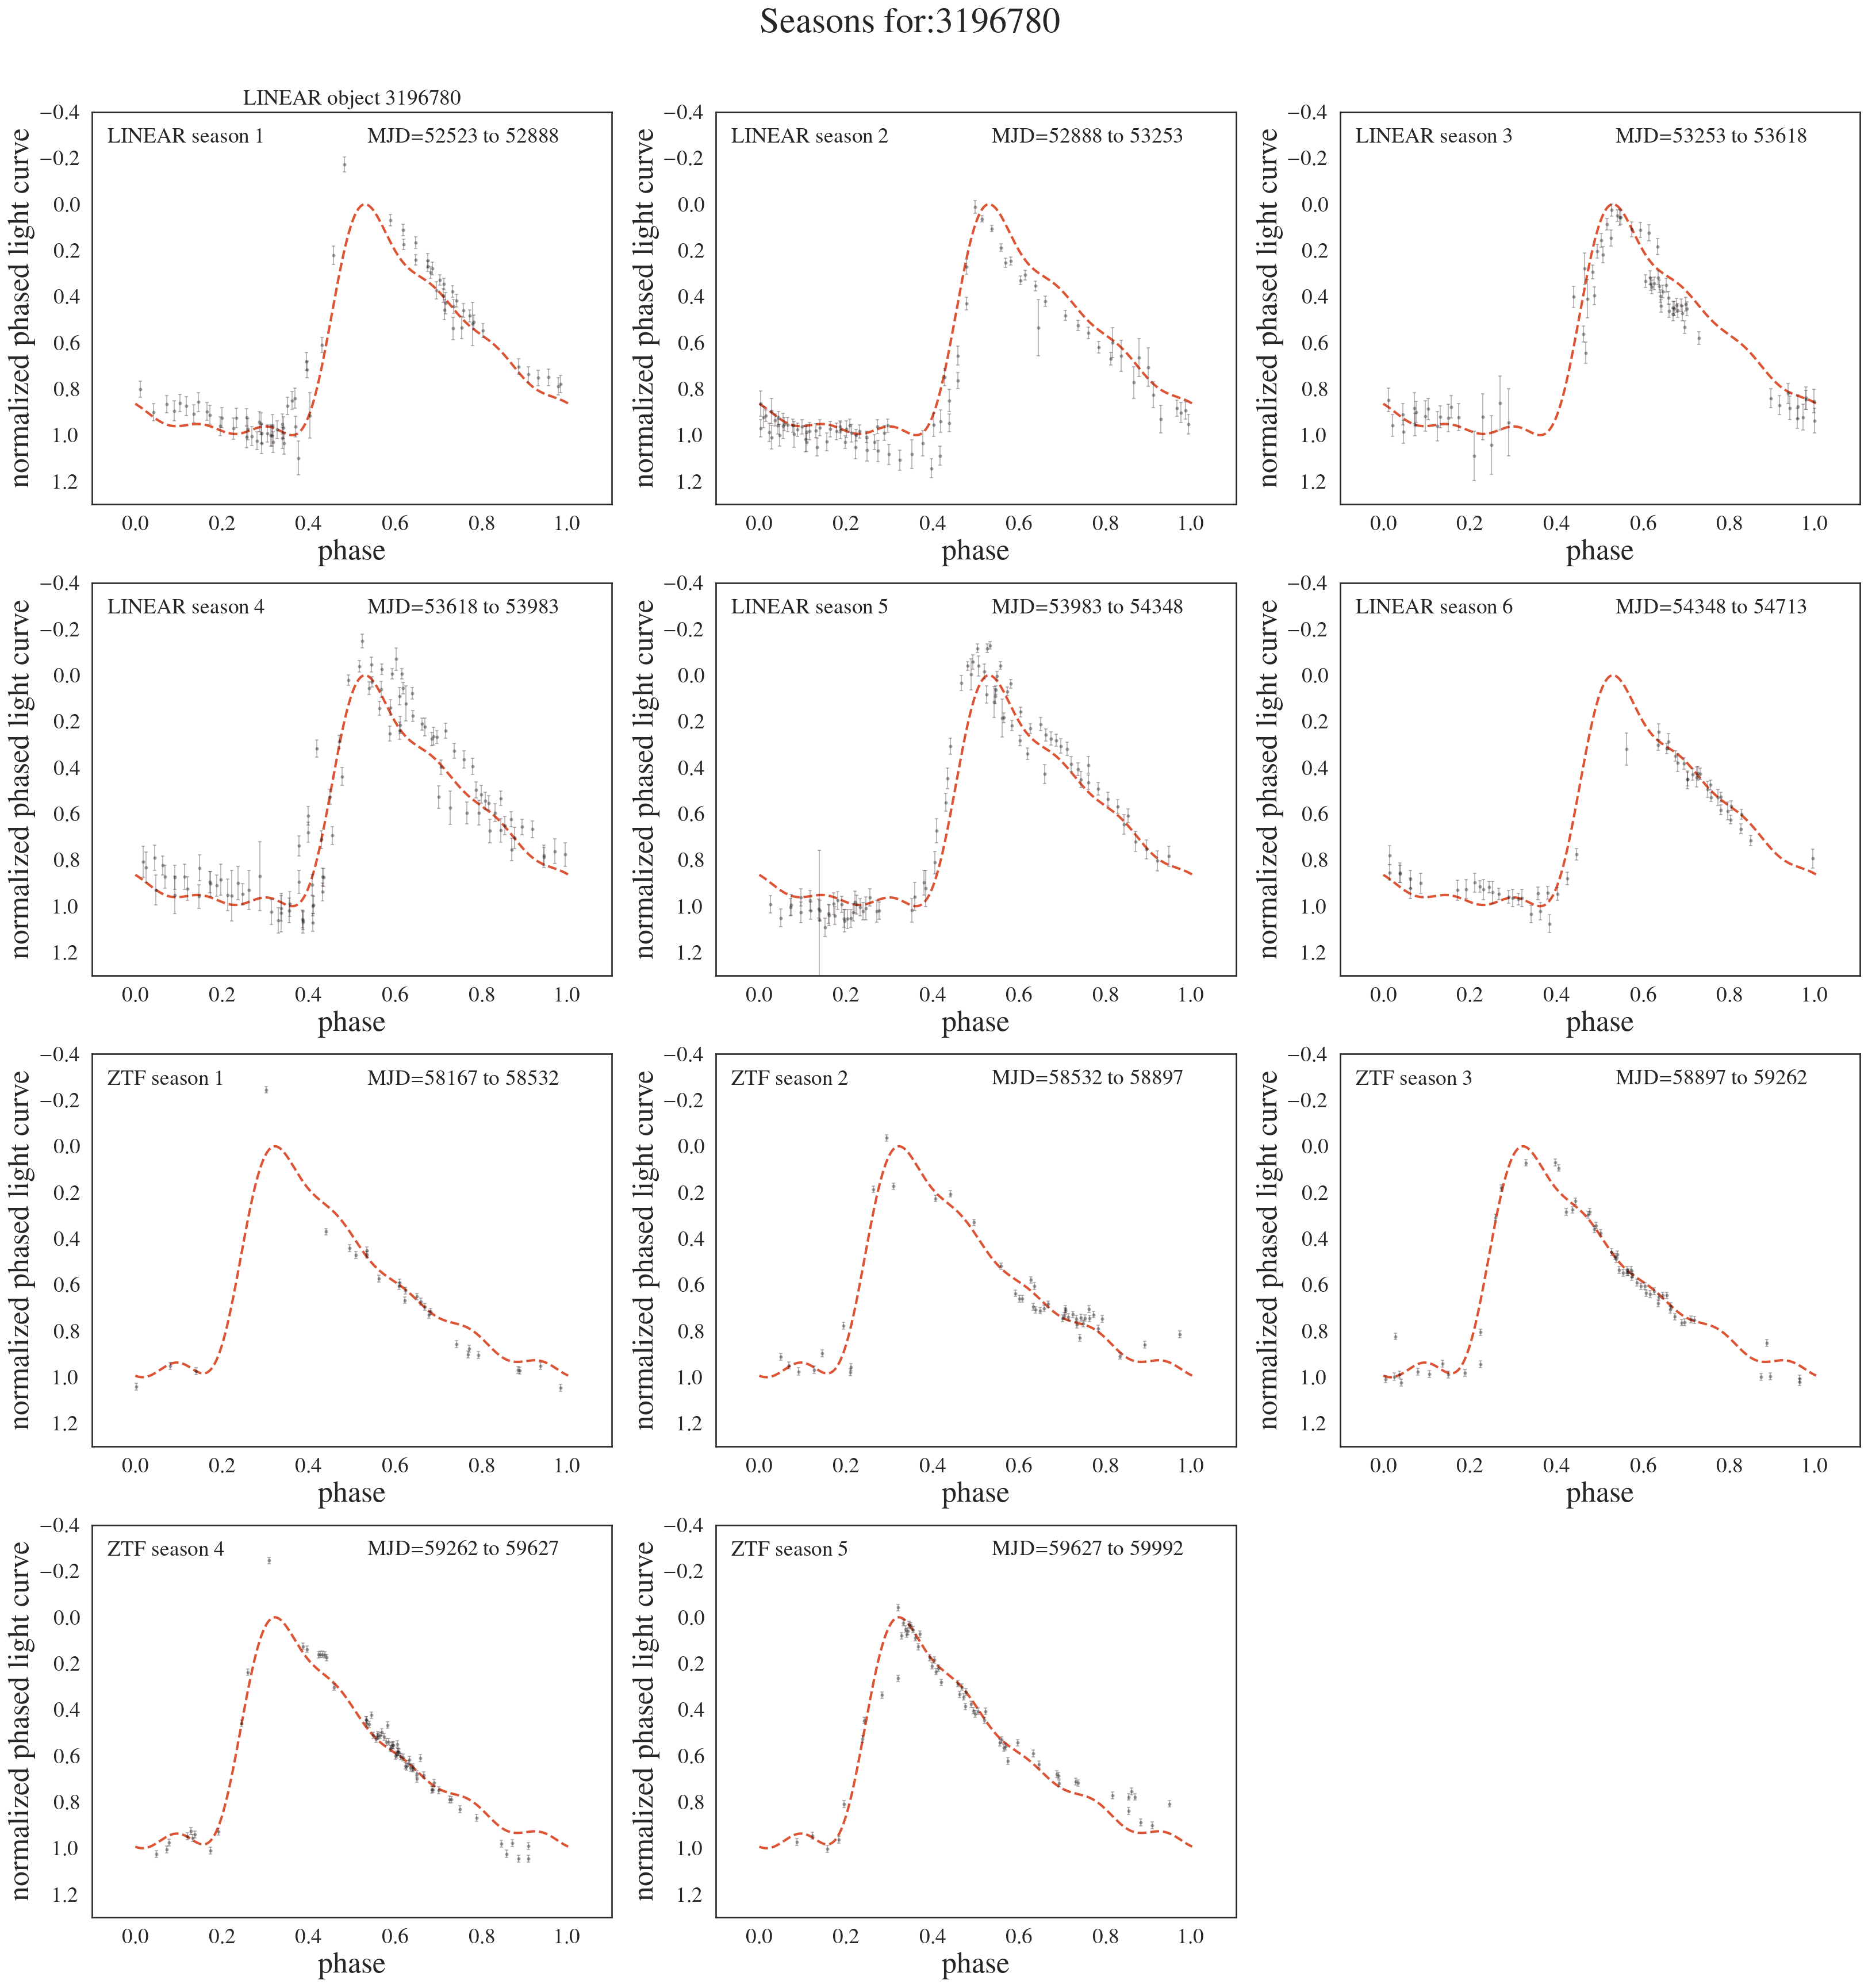
\includegraphics[width=16cm]{3196780_sn.png}}
    \caption{Analogous to Fig.~\ref{fig:phase4}, except that star
    with LINEARid = 3196780 is shown. Amplitude modulation is clearly
    seen in LINEAR light curves (top two rows), while not discernible
    in ZTF light curves (bottom two rows). Additional stars with
    similar behavior include LINEARid = 2889542, 7723614, 8342007.
    This behavior strongly  suggests that Blazhko effect can appear and disappear on time scales shorter than
      about a decade.
      }
      \label{fig:phase6}
\end{figure*}


During visual analysis, we noticed that some Blazhko stars exhibit
convincing Blazhko effect either in LINEAR or in ZTF data, but not in
both surveys. Fig.~\ref{fig:phase6} shows an example where amplitude
modulation is clearly seen in LINEAR light curves, while not discernible
in ZTF light curves.  There are also examples of stars where Blazhko effect is evident in
ZTF but not in LINEAR data (e.g., LINEARid = 19466437, 14155360). 
This finding  strongly suggests that Blazhko effect can appear and disappear on time scales shorter than
about a decade.

 

\section{Discussion and Conclusions\label{sec:discussion}}

We found excellent agreement
between the best-fit periods for RR Lyrae stars estimated separately from LINEAR and ZTF light curves. 
The sample of 228 stars presented here nearly doubles the number of field RR Lyrae stars displaying the Blazhko
effect and  places a lower limit of (11.4$\pm$0.8)\% for their incidence rate. 
The reported incidence rates for the Blazhko effect
range from 5\% \citep{2007MNRAS.377.1263S} to 60\% \citep{2014A&A...570A.100S}.
Differences in reported incidence rates can occur due to varying data precision, the temporal baseline length, and differences in visual or algorithmic analysis.
For a relatively small sample of
151 stars with Kepler data, a claim has been made that essentially every RR Lyrae star exhibits modulated light curve
\citep{2018A&A...614L...4K}. The difference in Blazhko incidence rates for the two most extensive samples, obtained
by the OGLE-III survey for the Large Magellanic Cloud (LMC, 20\% out of 17,693 stars; \citealt{2009AcA....59....1S})
and the Galactic bulge (30\% out of 11,756 stars; \citealt{2011AcA....61....1S}) indicates a possible variation of
the Blazhko incidence rate with underlying stellar population properties. 
 
We find that ab type RR Lyrae which show the Blazhko effect have about 5\% (0.030 day) shorter periods than starting
sample. While not large, the statistical significance of this difference is 7.1$\sigma$. At a similar uncertainty level
($\sim$1\%), we don't detect period difference for c type stars, and don't detect any difference in amplitude distributions.
We also find that for some stars the Blazhko effect is discernible in only one dataset. This finding  strongly suggests that Blazhko effect can
appear and disappear on time scales shorter than about a decade, in agreement with literature 
\citep{2009MNRAS.400.1006J, 2010A&A...520A.108P, 2014ApJS..213...31B}. 


The LINEAR and ZTF datasets analyzed in this work were sufficiently large that we had to rely on algorithmic
pruning of the initial sample. The sample size problem will be even larger for surveys such as the Legacy Survey
of Space and Time (LSST; \citealt{2019ApJ...873..111I}). LSST will be an excellent survey for studying Blazhko effect
\citep{2022ApJS..258....4H} because it will have both a long temporal baseline (10 years) and a large number of
observations per object (nominally 825; LSST Science Requirements Document\footnote{Available as ls.st/srd}).
We anticipate a higher fraction of discovered Blazhko stars with LSST than reported here due to better sampling
and superior photometric quality, since the incidence rate of the Blazhko effect increases with sensitivity to
small-amplitude modulation, and thus with photometric data quality \citep{2009MNRAS.400.1006J}.

The size and quality of LSST sample will motivate further developments of the selection algorithms. 
One obvious improvement will be inspection of neighboring objects to confirm photometric quality,
as well as inspection of images to test implication of an isolated point source (e.g., blended object photometry
can be affected by variable seeing beyond aperture correction valid for isolated point sources). 
Another improvement is forward modeling of the Blazhko modulation, rather than searching for $\chi^2$
outliers \citep{2011MNRAS.417..974B, 2012MNRAS.424..649G}.
For example, \cite{2020MNRAS.494.1237S} classified Blazhko stars in 6 classes using the morphology
of their amplitude modulation (the most dominant class includes 90\% of the sample). They also found bimodal distribution
of Blazko periods, with two components centered on 48 d and 186 d. These results give hope that forward
modeling of the Blazhko effect will improve the selection of such stars.
 
 


\begin{acknowledgements}

We thank Mathew Graham for providing {\it ztfquery} code example to us. 
\v{Z}.I. acknowledges funding by the Fulbright Foundation and thanks the Ru\d er Bo\v{s}kovi\'{c} Institute (Zagreb, Croatia) for hospitality.

Based on observations obtained with the Samuel Oschin Telescope 48-inch and the 60-inch Telescope at the Palomar Observatory as part of the Zwicky Transient Facility project. ZTF is supported by the National Science Foundation under Grants No. AST-1440341 and AST-2034437 and a collaboration including current partners Caltech, IPAC, the Weizmann Institute of Science, the Oskar Klein Center at Stockholm University, the University of Maryland, Deutsches Elektronen-Synchrotron and Humboldt University, the TANGO Consortium of Taiwan, the University of Wisconsin at Milwaukee, Trinity College Dublin, Lawrence Livermore National Laboratories, IN2P3, University of Warwick, Ruhr University Bochum, Northwestern University and former partners the University of Washington, Los Alamos National Laboratories, and Lawrence Berkeley National Laboratories. Operations are conducted by COO, IPAC, and UW.

The LINEAR program is funded by the National Aeronautics and Space Administration at MIT Lincoln Laboratory under Air Force Contract FA8721-05-C-0002.
Opinions, interpretations, conclusions and recommendations are those of the authors and are not necessarily endorsed by the United States Government.

\end{acknowledgements}

\newpage
\bibliographystyle{aa} % style aa.bst
\bibliography{paper} % your references Yourfile.bib


\onecolumn
\begin{appendix}
\section{Full table of results}
Here we present all the confirmed Blazhko stars with their LINEAR IDs, equatorial coordinates, and calculated periods and $\chi^2$ values.
%\begin{longtable}{lrrrrrrr}
    \toprule
    LINEAR ID & RA & DEC & LINEAR period & ZTF period & LINEAR chi-2 & ZTF chi-2 \\
        \midrule
    \endfirsthead
    
    \toprule
    LINEAR ID & RA & DEC & LINEAR period & ZTF period & LINEAR chi-2 & ZTF chi-2 \\
    \midrule
    \endhead
    
    \midrule
    \endfoot
    
    \bottomrule
    \endlastfoot
    
    523832 & 207.529404 & 33.706001 & 0.372376 & 0.372384 & 1.20 & 1.10 \\
1240665 & 206.202469 & 34.058662 & 0.632528 & 0.632522 & 3.00 & 1.10 \\
1736308 & 206.096115 & 36.648674 & 0.555848 & 0.555843 & 1.30 & 1.00 \\
2669011 & 206.229523 & 38.758453 & 0.591153 & 0.591151 & 1.10 & 0.70 \\
2742032 & 207.355225 & 39.589951 & 0.629676 & 0.629692 & 0.90 & 1.40 \\
2812086 & 206.805511 & 40.859066 & 0.646015 & 0.646000 & 3.00 & 3.20 \\
3507643 & 206.557358 & 39.536449 & 0.801141 & 0.801132 & 1.60 & 0.90 \\
5931160 & 207.177231 & 41.918797 & 0.664700 & 0.664708 & 0.80 & 1.10 \\
6665721 & 206.020233 & 41.646141 & 0.643318 & 0.643325 & 1.00 & 1.70 \\
17185566 & 206.387268 & 43.314617 & 0.614160 & 0.614169 & 1.50 & 1.90 \\
22828215 & 206.657028 & 43.543236 & 0.574536 & 0.574535 & 1.50 & 1.40 \\
29848 & 206.917358 & 44.971054 & 0.557020 & 0.557040 & 1.40 & 3.50 \\
158779 & 207.772202 & 45.916824 & 0.609207 & 0.609189 & 1.60 & 3.90 \\
263541 & 207.172470 & 45.713154 & 0.558218 & 0.558221 & 2.90 & 6.60 \\
514883 & 206.594757 & 46.482040 & 0.557723 & 0.557737 & 1.70 & 5.50 \\
737951 & 206.435547 & 45.881615 & 0.357023 & 0.357023 & 2.20 & 6.70 \\
810169 & 169.297485 & 6.265203 & 0.465185 & 0.465212 & 2.10 & 2.80 \\
924301 & 169.713531 & 6.963072 & 0.507503 & 0.507440 & 1.90 & 9.30 \\
1092244 & 207.060974 & 5.649392 & 0.649496 & 0.649558 & 1.20 & 3.60 \\
1244554 & 206.944962 & 5.346962 & 0.536875 & 0.536962 & 1.80 & 2.30 \\
1307948 & 206.223587 & 6.741248 & 0.527474 & 0.527415 & 1.80 & 4.50 \\
1332201 & 207.992432 & -4.603579 & 0.580711 & 0.580731 & 1.60 & 4.20 \\
1390653 & 207.220245 & -3.214271 & 0.521867 & 0.521871 & 1.30 & 4.10 \\
1435279 & 207.824600 & -3.712567 & 0.381858 & 0.381860 & 2.10 & 4.20 \\
1448299 & 206.582916 & 51.406654 & 0.606912 & 0.606940 & 2.70 & 5.40 \\
1593736 & 169.096771 & 5.428976 & 0.592628 & 0.592650 & 1.20 & 5.70 \\
1748058 & 207.353790 & 53.020401 & 0.310237 & 0.310176 & 1.40 & 5.70 \\
1857382 & 206.026001 & 56.421604 & 0.566428 & 0.566407 & 2.70 & 2.50 \\
1882354 & 207.117645 & 56.313797 & 0.695061 & 0.695029 & 1.50 & 2.80 \\
2041979 & 206.848053 & 55.248009 & 0.653694 & 0.653639 & 1.20 & 5.30 \\
2075949 & 207.733643 & 62.320267 & 0.477806 & 0.477666 & 1.60 & 4.70 \\
2117028 & 207.188278 & 61.978554 & 0.591245 & 0.591243 & 2.20 & 3.50 \\
2122319 & 206.210190 & 62.778843 & 0.359422 & 0.359424 & 2.10 & 6.10 \\
2229607 & 207.042603 & 65.877083 & 0.575179 & 0.575211 & 1.20 & 4.40 \\
2243683 & 206.780823 & 8.893113 & 0.579777 & 0.579803 & 3.10 & 4.30 \\
2248787 & 206.407776 & 7.914382 & 0.563528 & 0.563539 & 2.10 & 2.40 \\
2334384 & 206.454544 & 7.380644 & 0.555341 & 0.555333 & 2.00 & 6.50 \\
2397296 & 168.680649 & 51.998081 & 0.488814 & 0.488836 & 1.20 & 6.60 \\
2414841 & 206.101624 & 7.666218 & 0.559611 & 0.559592 & 1.70 & 5.70 \\
2455568 & 168.211075 & 51.534416 & 0.594119 & 0.594092 & 2.00 & 2.10 \\
2612592 & 207.693237 & -5.975360 & 0.571562 & 0.571543 & 1.30 & 2.80 \\
2653982 & 168.135025 & 51.014339 & 0.607082 & 0.607110 & 1.00 & 2.10 \\
2766997 & 207.782440 & -7.099904 & 0.289881 & 0.289943 & 1.80 & 3.60 \\
2892940 & 209.495773 & 2.587467 & 0.539855 & 0.539896 & 1.30 & 4.20 \\
3036295 & 209.338211 & 2.393512 & 0.629705 & 0.629714 & 1.80 & 2.20 \\
3140139 & 208.758163 & -0.100046 & 0.304590 & 0.304585 & 2.50 & 5.60 \\
3183285 & 208.391159 & 0.479103 & 0.349653 & 0.349664 & 1.20 & 2.80 \\
3196582 & 208.521881 & 0.740297 & 0.268017 & 0.268018 & 2.50 & 3.40 \\
3196780 & 169.384384 & 53.303658 & 0.504148 & 0.504199 & 2.20 & 3.20 \\
3294319 & 169.550766 & 53.459976 & 0.555460 & 0.555473 & 1.90 & 4.70 \\
3437725 & 208.845749 & 12.514306 & 0.542457 & 0.542478 & 1.50 & 6.30 \\
3591037 & 208.146072 & 14.167974 & 0.558643 & 0.558609 & 1.30 & 3.50 \\
3941776 & 209.073120 & 13.401526 & 0.532222 & 0.532209 & 2.80 & 6.00 \\
4101289 & 209.351425 & 13.537904 & 0.379225 & 0.379250 & 1.20 & 2.70 \\
4586691 & 208.326218 & 15.475822 & 0.621459 & 0.621446 & 2.00 & 3.40 \\
4804945 & 209.674210 & 16.421736 & 0.556172 & 0.556217 & 2.50 & 7.80 \\
5421989 & 208.014435 & 18.561077 & 0.534510 & 0.534527 & 0.80 & 2.50 \\
6582265 & 209.421219 & 17.441139 & 0.691751 & 0.691749 & 2.90 & 3.70 \\
6651516 & 208.909760 & 17.881287 & 0.308488 & 0.308496 & 1.30 & 5.80 \\
6819457 & 209.491974 & 20.296762 & 0.436282 & 0.436265 & 3.60 & 9.60 \\
6883239 & 208.333481 & 19.276327 & 0.563711 & 0.563712 & 2.90 & 2.50 \\
6967017 & 208.406662 & 21.846382 & 0.529691 & 0.529677 & 2.30 & 6.90 \\
7048826 & 208.492981 & 22.591896 & 0.317781 & 0.317790 & 1.40 & 5.90 \\
7254801 & 209.648148 & 22.561989 & 0.561133 & 0.561071 & 1.30 & 5.50 \\
7279621 & 208.915436 & 24.833937 & 0.415469 & 0.415467 & 1.90 & 4.60 \\
7283275 & 208.409698 & 26.350325 & 0.543342 & 0.543331 & 2.20 & 3.60 \\
7344401 & 209.188583 & 26.111385 & 0.330201 & 0.330226 & 1.80 & 2.70 \\
7580734 & 209.349243 & 26.322409 & 0.314956 & 0.314957 & 2.00 & 4.00 \\
7657340 & 208.098282 & 27.700201 & 0.495480 & 0.495493 & 2.30 & 4.00 \\
7811366 & 208.457687 & 30.868412 & 0.489523 & 0.489521 & 2.00 & 4.70 \\
7827663 & 208.047531 & 30.799057 & 0.390832 & 0.390832 & 3.40 & 4.50 \\
7846640 & 209.106400 & 4.330462 & 0.551495 & 0.551518 & 1.50 & 9.20 \\
8222011 & 209.258850 & 3.100914 & 0.350920 & 0.350914 & 2.00 & 4.80 \\
8311517 & 208.212936 & 4.452833 & 0.523354 & 0.523359 & 1.80 & 3.60 \\
8331094 & 208.446945 & 3.969552 & 0.267543 & 0.267549 & 2.10 & 3.30 \\
8343291 & 208.919601 & -2.689821 & 0.569785 & 0.569791 & 3.30 & 5.10 \\
9063194 & 169.357468 & 57.331566 & 0.575781 & 0.575760 & 2.40 & 3.10 \\
9236215 & 209.009872 & -1.607280 & 0.352570 & 0.352572 & 1.80 & 2.80 \\
9449335 & 209.488937 & -2.928472 & 0.475720 & 0.475695 & 2.00 & 5.00 \\
9532981 & 168.695602 & 60.104759 & 0.591000 & 0.591042 & 1.70 & 6.20 \\
9918809 & 209.255295 & -2.089725 & 0.479460 & 0.479509 & 1.90 & 11.60 \\
9968431 & 209.717804 & -2.437493 & 0.302266 & 0.302211 & 1.70 & 2.20 \\
9979905 & 208.905365 & 31.572962 & 0.338739 & 0.338739 & 2.50 & 2.30 \\
10030349 & 209.547668 & 32.537975 & 0.545073 & 0.545074 & 2.10 & 4.40 \\
10260828 & 208.891602 & 32.249817 & 0.380655 & 0.380643 & 2.20 & 7.40 \\
10814742 & 209.570526 & 31.039347 & 0.462687 & 0.462683 & 2.50 & 4.30 \\
11215595 & 208.180191 & 33.574619 & 0.546960 & 0.546943 & 1.30 & 2.30 \\
16991760 & 209.105652 & 33.977589 & 0.549098 & 0.549096 & 2.90 & 3.70 \\
17247918 & 169.489120 & 59.391106 & 0.481867 & 0.481865 & 1.80 & 4.60 \\
17275627 & 208.806717 & 33.957424 & 0.537775 & 0.537771 & 2.10 & 4.80 \\
17302403 & 209.807205 & 35.285717 & 0.488261 & 0.488343 & 2.00 & 6.40 \\
17544856 & 208.748581 & 36.859768 & 0.614297 & 0.614296 & 2.00 & 3.40 \\
19775800 & 208.958618 & 36.484657 & 0.310856 & 0.310867 & 1.30 & 2.70 \\
21488669 & 209.334930 & 37.248749 & 0.501644 & 0.501661 & 1.90 & 5.70 \\
21556651 & 208.269577 & 38.000725 & 0.614826 & 0.614808 & 1.80 & 3.10 \\
21619184 & 208.125366 & 37.095997 & 0.557343 & 0.557320 & 2.30 & 3.70 \\
21806402 & 208.151657 & 39.543987 & 0.592081 & 0.592104 & 1.60 & 6.20 \\
21874209 & 209.602371 & 40.245346 & 0.611295 & 0.611286 & 2.50 & 5.90 \\
21967825 & 209.202347 & 39.452202 & 0.540607 & 0.540600 & 1.80 & 4.70 \\
22244513 & 208.742203 & 41.386112 & 0.604149 & 0.604077 & 2.50 & 8.10 \\
22319996 & 209.734711 & 42.773571 & 0.479505 & 0.479495 & 2.60 & 4.90 \\
22518636 & 208.239105 & 41.299026 & 0.283996 & 0.283998 & 1.80 & 3.00 \\
22959674 & 209.018127 & 41.835575 & 0.405333 & 0.405409 & 1.80 & 3.80 \\
22980793 & 208.105713 & 44.400867 & 0.540348 & 0.540353 & 1.90 & 2.80 \\
23135759 & 209.604721 & 45.746510 & 0.402730 & 0.402732 & 4.20 & 4.40 \\
23148883 & 209.446594 & 45.757584 & 0.390130 & 0.390124 & 1.40 & 4.80 \\
23184808 & 208.547745 & 47.825001 & 0.338821 & 0.338888 & 1.00 & 5.70 \\
23193507 & 208.703445 & 49.226929 & 0.473158 & 0.473174 & 3.40 & 4.60 \\
23653629 & 209.116013 & 50.653641 & 0.442052 & 0.442055 & 2.40 & 4.40 \\
24019356 & 208.649506 & 50.454273 & 0.517473 & 0.517460 & 1.50 & 4.60 \\
24020106 & 209.853088 & 5.836339 & 0.542397 & 0.542396 & 2.90 & 4.50 \\
24216004 & 209.385406 & 6.251467 & 0.382077 & 0.381912 & 1.90 & 7.80 \\
880588 & 208.532242 & 6.762656 & 0.600138 & 0.600134 & 1.20 & 2.40 \\
1212611 & 208.592422 & 6.144436 & 0.630896 & 0.630893 & 0.90 & 1.20 \\
1876491 & 209.131027 & 5.983884 & 0.760128 & 0.760123 & 1.20 & 1.20 \\
3048546 & 209.125137 & -4.194337 & 0.656287 & 0.656293 & 1.00 & 1.30 \\
5272753 & 208.115189 & -4.847239 & 0.485827 & 0.485831 & 0.90 & 1.60 \\
8610884 & 208.744736 & -4.852155 & 0.592421 & 0.592429 & 2.20 & 4.30 \\
8907563 & 209.521454 & -3.322183 & 0.513164 & 0.513164 & 1.10 & 4.60 \\
9852554 & 208.390961 & -4.619442 & 0.651339 & 0.651367 & 1.00 & 4.50 \\
9961135 & 209.178848 & 52.903030 & 0.590896 & 0.590891 & 1.10 & 1.80 \\
10503746 & 208.417831 & 54.266953 & 0.573563 & 0.573570 & 2.70 & 1.90 \\
21948290 & 209.862518 & 56.455978 & 0.511127 & 0.511115 & 2.30 & 2.40 \\
23596342 & 209.988663 & 56.828396 & 0.602841 & 0.602846 & 1.20 & 2.90 \\
23898397 & 121.150764 & 42.483574 & 0.563018 & 0.562989 & 1.60 & 3.50 \\
1882088 & 208.323578 & 58.245502 & 0.315984 & 0.316041 & 4.00 & 1.50 \\
2936953 & 208.351578 & 57.226521 & 0.328746 & 0.328733 & 2.70 & 1.30 \\
3219035 & 209.858856 & 60.601982 & 0.326746 & 0.326509 & 3.90 & 2.60 \\
4320492 & 168.062149 & 65.801857 & 0.361005 & 0.360942 & 3.70 & 1.80 \\
8036191 & 208.732498 & 59.448402 & 0.363860 & 0.363893 & 2.20 & 1.60 \\
10420063 & 209.945786 & 61.264187 & 0.487395 & 0.487394 & 4.20 & 3.70 \\
10662468 & 209.124405 & 61.076996 & 0.445180 & 0.445167 & 3.60 & 1.80 \\
21688272 & 209.311371 & 62.800976 & 0.304803 & 0.304790 & 2.30 & 1.80 \\
2714034 & 168.354202 & 65.678604 & 0.610868 & 0.610800 & 1.50 & 1.20 \\
5592590 & 208.440872 & 65.857277 & 0.346945 & 0.346980 & 1.20 & 1.10 \\
8799313 & 208.821136 & 7.846983 & 0.327560 & 0.327542 & 1.10 & 1.60 \\
\bottomrule
\end{longtable}
    
\begin{tabular}{rrrrrrrrrrrrrrrlrr}
\toprule
 LINEAR ID &  Plinear &       Pztf &  N\_L &  N\_Z &  L\_chi2r &  Z\_chi2r &  L\_chi2 &   Z\_chi2 &      Lampl &       Zampl &  BpeakL &  BpeakZ &  BperiodL &  BperiodZ & Periodogram\_f &  B\_score &  Blazhko\_f \\
\midrule
     29848 & 0.557020 &   0.557040 &  301 &   43 &      1.4 &      3.5 &     3.0 &     12.6 &       0.56 &        0.93 &  1.8328 &  1.7982 &   26.6205 &  333.3333 &             - &        6 &          1 \\
     50402 & 0.643303 &   0.643294 &  284 &  586 &      0.7 &      1.1 &     0.6 &      1.8 &       0.48 &        0.69 &  1.6223 &  1.5918 &   14.7351 &   26.8420 &             - &        0 &         -1 \\
     62892 & 0.530776 &   0.530785 &  276 &  771 &      0.9 &      3.2 &     1.1 &     19.8 &       0.62 &        0.64 &  1.9519 &  1.9433 &   14.7319 &   16.8634 &             - &        0 &         -1 \\
     91437 & 0.674733 &   0.674737 &  177 &  564 &      1.3 &      2.0 &     2.8 &      5.6 &       0.87 &        1.21 &  1.5498 &  1.4849 &   14.7580 &  355.8719 &             - &        0 &         -1 \\
     95250 & 0.313870 &   0.313876 &  222 &  916 &      0.8 &      1.4 &     0.8 &      3.0 &       0.48 &        0.46 &  3.2565 &  3.1889 &   14.1844 &  342.4658 &             - &        0 &         -1 \\
    104455 & 0.997195 &   0.997587 &  119 &   44 &      1.6 &     17.6 &     3.4 &    184.1 &    4141.12 &    42446.41 &  1.0058 &  1.0499 &  336.1345 &   21.0682 &             - &        0 &         -1 \\
    108513 & 0.473809 &   1.000362 &  282 &   42 &      1.4 &     10.9 &     4.0 &    161.1 &       0.86 &    26072.93 &  2.1465 &  1.0034 &   27.8203 &  266.3116 &             - &        0 &         -1 \\
    136668 & 0.532923 &   0.532929 &  310 &  918 &      1.1 &      2.3 &     1.6 &     17.0 &       0.82 &        0.78 &  1.9095 &  1.9396 &   30.2847 &   15.8391 &             - &        0 &         -1 \\
    141414 & 0.335690 &   0.335669 &  278 &  919 &      0.8 &      1.5 &     0.6 &      2.6 &       0.41 &        0.37 &  3.0467 &  2.9930 &   14.7504 &   71.8907 &             - &        0 &         -1 \\
    142794 & 0.470787 &   0.470802 &  270 &   63 &      1.0 &      2.3 &     1.8 &     11.9 &       0.72 &        0.72 &  2.1848 &  2.1851 &   16.4880 &   16.3626 &             - &        0 &         -1 \\
    158779 & 0.609207 &   0.609189 &  293 &  616 &      1.6 &      3.9 &     3.7 &     34.2 &       0.47 &        0.68 &  1.6443 &  1.6444 &  352.7337 &  350.2627 &             - &        6 &          1 \\
    162255 & 0.512747 &   0.512744 &  266 & 1119 &      1.6 &      1.6 &     5.7 &      6.2 &       0.96 &        1.31 &  1.9531 &  1.9765 &  355.8719 &   38.1243 &             - &        0 &         -1 \\
    163933 & 0.339629 &   0.679246 &  306 &   53 &      0.9 &      0.9 &     1.0 &      1.5 &       0.45 &        0.35 &  2.9472 &  1.5272 &  353.3569 &   18.1802 &             - &        0 &         -1 \\
    172382 & 0.458309 &   0.458308 &  227 & 1461 &      1.1 &      2.4 &     1.5 &     10.2 &       1.16 &        1.10 &  2.2435 &  2.2716 &   16.2536 &   11.1595 &             - &        0 &         -1 \\
    174389 & 0.334036 &   0.334040 &  270 &  786 &      1.4 &      1.4 &     4.5 &      2.2 &       0.27 &        0.33 &  3.0643 &  2.9968 &   14.1693 &  320.0000 &             - &        0 &         -1 \\
    186102 & 0.647419 &   0.647425 &  188 &  574 &      0.7 &      1.3 &     0.6 &      2.6 &       0.89 &        1.11 &  1.5889 &  1.5501 &   22.5785 &  182.1494 &             - &        0 &         -1 \\
    215632 & 0.572162 &   0.572163 &  286 &  441 &      1.0 &      1.4 &     0.9 &      3.4 &       0.75 &        0.99 &  1.8182 &  1.7507 &   14.1975 &  336.7003 &             - &        0 &         -1 \\
    258499 & 0.401505 &   0.401504 &  275 &  537 &      1.5 &      1.6 &     2.7 &      2.9 &       0.34 &        0.36 &  2.5613 &  2.5182 &   14.1413 &   36.2384 &             - &        0 &         -1 \\
    263541 & 0.558218 &   0.558221 &  270 &  503 &      2.9 &      6.6 &    15.8 &    110.4 &       0.64 &        0.82 &  1.8621 &  1.8025 &   14.1513 &   89.9685 &             - &        7 &          1 \\
    303860 & 0.499321 &   0.492164 &  280 &  639 &      5.0 &      4.3 &    36.3 &     83.8 &      86.75 &        1.08 &  2.0319 &  2.0464 &   34.3053 &   68.7049 &             - &        0 &         -1 \\
    309626 & 0.595841 &   0.997215 &  215 &   40 &      2.9 &     16.5 &    21.0 &    445.4 &       0.68 &   868885.53 &  1.6811 &  1.0305 &  353.3569 &   36.1011 &             - &        0 &         -1 \\
    355767 & 0.499298 &   0.521363 &  180 &  114 &      3.4 &      1.8 &     9.5 &      4.5 &    4622.25 &        1.12 &  2.0132 &  1.9240 &   95.9693 &  167.2241 &             - &        0 &         -1 \\
    393084 & 0.530027 &   0.530033 &  493 &  372 &      1.1 &      3.2 &     1.6 &     19.2 &       0.96 &        1.31 &  1.9447 &  1.8896 &   17.2369 &  347.2222 &             - &        0 &         -1 \\
    418785 & 0.700122 &   0.700120 &  263 &   50 &      0.8 &      0.9 &     1.4 &      1.3 &       0.56 &        0.44 &  1.4770 &  1.4685 &   20.5508 &   24.9066 &             - &        0 &         -1 \\
    420327 & 0.535225 &   0.535220 &  144 &  656 &      0.8 &      1.4 &     1.1 &      2.8 &       0.53 &        0.74 &  1.9020 &  1.8713 &   29.7177 &  345.4231 &             - &        0 &         -1 \\
    437483 & 0.699234 &   0.699235 &  316 &  666 &      0.7 &      1.0 &     0.5 &      1.7 &       0.37 &        0.35 &  1.4640 &  1.4385 &   29.4942 &  119.9041 &             - &        0 &         -1 \\
    439441 & 0.709248 &   0.709247 &  349 &  443 &      1.3 &      1.4 &     2.1 &      2.4 &       0.36 &        0.50 &  1.4718 &  1.4136 &   16.1603 &  271.3704 &             - &        0 &         -1 \\
    514883 & 0.557723 &   0.557737 &  289 &  555 &      1.7 &      5.5 &     5.3 &     53.7 &       0.55 &        0.72 &  1.8472 &  1.7958 &   18.4655 &  357.1429 &             - &        7 &          1 \\
    516954 & 0.297570 &   0.297569 &  243 & 1164 &      2.3 &      1.3 &     5.6 &      2.7 &       0.52 &        0.60 &  3.4523 &  3.3634 &   10.8962 &  357.7818 &             - &        0 &         -1 \\
    523832 & 0.372376 &   0.372384 &  251 &   42 &      1.2 &      1.1 &     1.8 &      0.8 &       0.42 &        0.59 &  2.8040 &  2.7122 &    8.4370 &   37.3413 &             Z &        0 &          2 \\
    558961 & 0.600532 &   0.600547 &  213 &   61 &      2.2 &      1.7 &    11.9 &      2.0 &       0.55 &        0.55 &  1.7357 &  1.6680 &   14.1753 &  352.1127 &             - &        0 &         -1 \\
    608497 & 0.485636 &   0.748671 &  556 &   37 &      2.5 &     10.5 &    20.4 &    504.9 &       0.86 &       19.10 &  2.0930 &  1.3432 &   29.5290 &  133.6898 &             - &        0 &         -1 \\
    658512 & 0.969050 &   2.708902 &  404 &   42 &      1.5 &      5.4 &     2.4 &     25.0 &       0.31 &        0.67 &  1.0479 &  0.3806 &   62.7549 &   87.2981 &             - &        0 &         -1 \\
    664583 & 0.602994 &   0.603021 &  449 &  613 &      1.1 &      2.5 &     1.8 &     11.1 &       0.56 &        0.53 &  1.6612 &  1.6666 &  357.7818 &  120.4094 &             - &        0 &         -1 \\
    670864 & 0.600802 &   0.395810 &  336 &   42 &      0.9 &     10.6 &     1.2 &    115.1 &       0.52 &       23.53 &  1.7415 &  2.5564 &   12.9811 &   33.3667 &             - &        0 &         -1 \\
    717668 & 0.426744 &   0.426758 &  302 &  428 &      1.2 &      1.7 &     1.6 &      3.9 &       0.32 &        0.32 &  2.4138 &  2.3515 &   14.1834 &  121.2856 &             - &        0 &         -1 \\
    734545 & 0.289482 &   0.702579 &  305 &   41 &      1.7 &      5.4 &     3.3 &     28.6 &       0.29 &        0.44 &  3.5249 &  1.4379 &   14.1874 &   68.7994 &             - &        0 &         -1 \\
    737951 & 0.357023 &   0.357023 &  273 &  871 &      2.2 &      6.7 &     6.0 &     42.4 &       0.43 &        0.34 &  2.8038 &  2.8039 &  353.3569 &  332.2259 &             - &        6 &          1 \\
    771232 & 0.540930 &   0.540941 &  301 &  889 &      1.0 &      1.6 &     1.1 &      4.7 &       0.93 &        0.89 &  1.9257 &  1.9257 &   12.9811 &   12.9744 &             - &        0 &         -1 \\
    798477 & 0.651627 &   0.651611 &  294 &  139 &      1.2 &      3.5 &     2.0 &     17.8 &       0.61 &        0.78 &  1.5984 &  1.6041 &   15.6838 &   14.3968 &             - &        0 &         -1 \\
    803829 & 0.595281 &   0.595286 &  270 &  561 &      2.3 &      2.6 &     8.7 &      9.9 &       0.91 &        1.34 &  1.7205 &  1.6828 &   24.5912 &  335.5705 &             - &       10 &          0 \\
    810169 & 0.465185 &   0.465212 &  289 &  743 &      2.1 &      2.8 &     6.0 &     15.1 &       0.77 &        0.75 &  2.2232 &  2.2230 &   13.6017 &   13.6082 &             - &       12 &          1 \\
    813450 & 0.589387 &   0.589389 &  221 &  431 &      1.3 &      1.0 &     2.0 &      2.3 &       0.70 &        0.93 &  1.7703 &  1.7022 &   13.5796 &  181.8182 &             - &        0 &         -1 \\
    836895 & 0.473399 &   0.473398 &  194 &  612 &      1.3 &      2.8 &     3.0 &     11.1 &       1.09 &        1.49 &  2.1672 &  2.1673 &   18.2415 &   18.2232 &             - &        0 &         -1 \\
    843294 & 0.374216 &   0.374214 &  290 &  358 &      1.4 &      1.7 &     3.3 &      5.1 &       0.36 &        0.36 &  2.7060 &  2.6778 &   29.6252 &  180.1802 &             - &        0 &         -1 \\
    851716 & 1.908191 &   0.388356 &  100 &  147 &      1.2 &      5.3 &     1.3 &     39.7 &       0.64 &        0.38 &  0.5241 &  2.5778 &    0.0000 &  354.6099 &             - &        0 &         -1 \\
    856862 & 0.625858 &   1.251798 &  294 &   26 &      1.0 &      1.2 &     1.1 &      1.6 &       0.45 &        0.60 &  1.6344 &  0.7989 &   27.3635 &    0.0000 &             - &        0 &         -1 \\
    869112 & 0.635690 &   1.753223 &  322 &   32 &      0.9 &      2.1 &     1.0 &      4.4 &       0.34 &        0.54 &  1.6071 &  0.5965 &   29.4118 &   38.2263 &             - &        0 &         -1 \\
    872620 & 0.549247 &   0.549248 &  282 &  272 &      1.0 &      1.5 &     1.1 &      2.8 &       0.85 &        0.63 &  1.8289 &  1.8303 &  121.2856 &  103.6269 &             - &        0 &         -1 \\
    880568 & 0.628261 &   1.157215 &  200 &   30 &      2.5 &      1.6 &    19.6 &     19.2 &       0.73 &        0.74 &  1.6509 &  0.8862 &   16.8805 &   45.3309 &             - &        0 &         -1 \\
    880588 & 0.600138 &   0.600134 &  295 &  442 &      1.2 &      2.4 &     3.2 &     23.4 &       0.91 &        0.84 &  1.6910 &  1.6736 &   40.5268 &  136.4256 &             L &        0 &          2 \\
    883073 & 0.725513 &   2.661727 &  302 &   32 &      1.0 &      2.9 &     1.0 &      9.5 &       0.43 &        0.61 &  1.4148 &  0.3853 &   27.4198 &  104.6572 &             - &        0 &         -1 \\
    895953 & 0.658156 &   0.658154 &  297 &  408 &      0.7 &      1.5 &     0.5 &      3.4 &       0.46 &        0.50 &  1.5528 &  1.5554 &   29.9760 &   27.7971 &             - &        0 &         -1 \\
    899832 & 0.589463 &  12.401002 &  285 &    6 &      2.1 &      0.2 &     9.3 &      0.0 &       0.61 &      255.00 &  1.7264 &  0.0806 &   33.4057 &    0.0000 &             - &        0 &         -1 \\
    924301 & 0.507503 &   0.507440 &  418 &  189 &      1.9 &      9.3 &    13.8 &    162.9 &       0.87 &        0.79 &  2.0043 &  1.9763 &   29.5072 &  178.4121 &             - &       10 &          1 \\
    966279 & 0.517279 &   0.517270 &  330 &  607 &      1.5 &      2.7 &     6.1 &     21.0 &       0.92 &        0.82 &  2.0010 &  2.0027 &   14.7406 &   14.3978 &             - &        0 &         -1 \\
    967924 & 0.643331 &   0.643319 &  227 &  569 &      0.9 &      1.4 &     0.7 &      3.0 &       0.92 &        1.27 &  1.6221 &  1.5592 &   14.7667 &  210.9705 &             - &        0 &         -1 \\
    968962 & 0.579336 &   0.579334 &  235 &  711 &      1.0 &      1.4 &     1.1 &      3.4 &       0.84 &        0.80 &  1.7934 &  1.7311 &   14.8644 &  199.2032 &             - &        0 &         -1 \\
    969277 & 1.003276 &   0.691657 &  220 &  676 &      2.8 &      1.2 &    13.0 &      2.5 &       0.55 &        0.75 &  0.9996 &  1.4508 &  344.8276 &  200.4008 &             - &        0 &         -1 \\
    970326 & 0.592233 &   0.592231 &  275 &  552 &      1.1 &      2.1 &     1.9 &      7.7 &       0.51 &        0.75 &  1.7563 &  1.6992 &   14.7656 &   93.2836 &             - &        0 &         -1 \\
    976746 & 0.620673 &   0.620663 &  236 &   91 &      1.6 &      1.4 &     3.9 &      2.3 &       0.45 &        0.40 &  1.6790 &  1.6844 &   14.7493 &   13.6603 &             - &        0 &         -1 \\
    989567 & 0.316227 &   0.632456 &  283 &   69 &      1.1 &      2.3 &     1.4 &      4.4 &       0.25 &        0.80 &  3.2300 &  1.6291 &   14.7601 &   20.8485 &             - &        0 &         -1 \\
    991055 & 0.347282 &   0.997648 &  131 &  104 &      1.3 &     12.2 &     2.7 &    130.4 &       0.43 &       16.81 &  3.0117 &  1.0072 &    7.5637 &  207.6843 &             - &        0 &         -1 \\
    993105 & 0.794678 &   0.794668 &  205 &  115 &      0.9 &      1.0 &     0.9 &      1.0 &       0.34 &        0.23 &  1.2963 &  1.2646 &   26.3401 &  161.4205 &             - &        0 &         -1 \\
    999528 & 0.658401 &   0.658407 &  564 &  213 &      1.2 &      2.7 &     1.8 &     21.7 &       0.57 &        0.92 &  1.5527 &  1.5510 &   29.5247 &   31.0366 &             - &        0 &         -1 \\
   1004849 & 0.458463 &   0.458467 &  607 &  193 &      1.3 &      2.6 &     6.5 &     14.7 &       1.14 &        1.60 &  2.2151 &  2.2704 &   29.4985 &   11.2039 &             - &        0 &         -1 \\
   1005497 & 0.653607 &   0.653605 &  607 &  192 &      1.1 &      2.1 &     2.1 &     12.4 &       0.60 &        0.83 &  1.5639 &  1.5481 &   29.4638 &   55.1116 &             - &        0 &         -1 \\
   1013889 & 0.504572 &   0.504520 &  228 &  106 &      1.3 &      4.4 &     3.8 &     28.0 &       0.72 &        0.49 &  2.0444 &  1.9924 &   15.9885 &   97.1345 &             - &        0 &         -1 \\
   1032186 & 0.997228 &   2.637662 &  140 &   21 &      2.3 &      6.4 &     4.5 &     31.5 &    3605.43 &     1144.44 &  1.0187 &  0.3910 &   62.9129 &   84.5309 &             - &        0 &         -1 \\
   1034627 & 0.620331 &   0.620278 &  167 &  585 &      1.3 &      3.2 &     4.9 &     18.3 &       0.37 &        0.34 &  1.6257 &  1.6187 &   73.2332 &  154.0832 &             - &        0 &         -1 \\
   1049602 & 0.302012 &   0.302016 &  220 &  475 &      1.4 &      1.1 &     2.3 &      1.4 &       0.39 &        0.37 &  3.3450 &  3.3159 &   29.4898 &  207.2539 &             - &        0 &         -1 \\
   1051321 & 0.330482 &   0.330481 &  558 &  353 &      1.2 &      1.3 &     5.6 &      1.9 &       0.33 &        0.33 &  3.0598 &  3.0314 &   29.5029 &  180.3427 &             - &        0 &         -1 \\
   1051858 & 0.632085 &   0.632085 &  552 &  276 &      0.7 &      1.1 &     0.6 &      1.2 &       0.38 &        0.53 &  1.6160 &  1.5853 &   29.4551 &  313.4796 &             - &        0 &         -1 \\
   1058132 & 0.632859 &   0.632854 &  607 &  187 &      0.8 &      1.0 &     0.8 &      1.6 &       0.44 &        0.59 &  1.6140 &  1.6005 &   29.5072 &   49.0798 &             - &        0 &         -1 \\
   1059786 & 0.463511 &   0.463516 &  549 &  350 &      1.0 &      2.0 &     1.4 &      8.0 &       1.18 &        1.15 &  2.1913 &  2.2348 &   29.5247 &   12.9241 &             - &        0 &         -1 \\
   1080552 & 0.702908 &   0.351453 &  548 &  291 &      2.5 &      8.1 &     8.2 &     75.1 &       0.42 &        0.49 &  1.4396 &  2.9255 &   59.1191 &   12.4774 &             - &        0 &         -1 \\
   1092244 & 0.649496 &   0.649558 &  590 &  326 &      1.2 &      3.6 &     2.3 &     32.1 &       0.72 &        0.58 &  1.5735 &  1.5640 &   29.5421 &   40.8330 &             - &        7 &          1 \\
   1102647 & 0.621541 &   0.621548 &  559 &  285 &      1.3 &      1.7 &     2.8 &      4.6 &       0.78 &        0.79 &  1.6428 &  1.6144 &   29.5116 &  180.9955 &             - &        0 &         -1 \\
   1111522 & 0.523951 &   0.499325 &  345 &  292 &      1.4 &     27.1 &     5.9 &    622.0 &       0.89 &      530.50 &  1.9570 &  2.0027 &   20.6356 &    0.0000 &             - &        0 &         -1 \\
   1112498 & 0.492932 &   0.492942 &  541 &  289 &      1.0 &      1.9 &     1.6 &      8.9 &       1.09 &        1.44 &  2.0416 &  2.0545 &   77.1903 &   38.6922 &             - &        0 &         -1 \\
   1113422 & 0.386238 &   1.638072 &  384 &   22 &      2.6 &      1.7 &     8.7 &     29.0 &       0.43 &       21.67 &  2.6255 &  0.6171 &   27.4348 &  150.1502 &             - &        0 &         -1 \\
   1124773 & 0.331832 &   0.663660 &  169 &  155 &      1.0 &      1.3 &     1.0 &      2.2 &       0.34 &        0.49 &  3.1227 &  1.5218 &    9.1617 &   66.4673 &             - &        0 &         -1 \\
   1127427 & 0.619895 &   0.619900 &  184 &  155 &      1.0 &      1.1 &     1.1 &      1.7 &       0.52 &        0.73 &  1.6298 &  1.6520 &   60.0240 &   25.7367 &             - &        0 &         -1 \\
   1128811 & 0.313351 &   0.313355 &  144 &  195 &      0.8 &      1.2 &     1.2 &      1.8 &       0.50 &        0.38 &  3.3003 &  3.1967 &    9.1705 &  184.1621 &             - &        0 &         -1 \\
   1130401 & 0.467372 &   0.467362 &  151 &  189 &      2.8 &      5.8 &    23.0 &     53.8 &       0.75 &        0.80 &  2.2293 &  2.1451 &   11.1539 &  182.6484 &             - &        0 &         -1 \\
   1132871 & 0.556640 &   0.556606 &  144 &  156 &      2.0 &      5.5 &     6.3 &     80.3 &       0.85 &        0.98 &  1.8021 &  1.8413 &  177.7778 &   22.3539 &             - &        0 &         -1 \\
   1145534 & 0.536989 &   1.627078 &  310 &   23 &      1.1 &      5.7 &     1.9 &     49.6 &       0.82 &       24.39 &  1.8963 &  0.6146 &   29.3815 &    0.0000 &             - &        0 &         -1 \\
   1152390 & 0.488849 &   0.488846 &  145 &  197 &      1.1 &      2.2 &     1.7 &      9.5 &       0.99 &        0.97 &  2.0484 &  2.0670 &  356.5062 &   46.7071 &             - &        0 &         -1 \\
   1169665 & 1.238946 &   0.412945 &  305 &  330 &      4.7 &      9.3 &    24.5 &     86.5 &       0.30 &        0.35 &  0.8342 &  2.4254 &   36.9481 &  261.7801 &             - &        0 &         -1 \\
   1179977 & 0.689492 &   2.234060 &  254 &   27 &      0.9 &      1.5 &     1.3 &     16.3 &       0.62 &        1.04 &  1.4862 &  0.4578 &   27.8629 &   98.6680 &             - &        0 &         -1 \\
   1197898 & 0.341894 &   0.341881 &  261 &  240 &      1.2 &      1.5 &     2.0 &      3.2 &       0.27 &        0.40 &  2.9953 &  2.9280 &   14.1995 &  333.3333 &             - &        0 &         -1 \\
   1210627 & 0.284468 &   0.284472 &  277 &  461 &      1.1 &      1.8 &     1.4 &      4.2 &       0.46 &        0.60 &  3.5860 &  3.5202 &   14.1553 &  205.1282 &             - &        0 &         -1 \\
   1212611 & 0.630896 &   0.630893 &  297 &  478 &      0.9 &      1.2 &     0.9 &      2.5 &       0.75 &        1.01 &  1.5962 &  1.6399 &   89.3256 &   18.2199 &             L &        0 &          2 \\
   1240665 & 0.632528 &   0.632522 &  468 &  311 &      3.0 &      1.1 &    25.2 &      1.6 &       0.33 &        0.33 &  1.6149 &  1.5865 &   29.4942 &  182.3154 &             Z &        0 &          2 \\
   1241164 & 0.428471 &   5.815305 &  626 &   13 &      1.3 &      0.1 &     4.9 &      0.2 &       0.32 &    17662.00 &  2.3678 &  0.1750 &   29.4898 &  325.2033 &             - &        0 &         -1 \\
   1244554 & 0.536875 &   0.536962 &  469 &  312 &      1.8 &      2.3 &     9.5 &     14.8 &       0.71 &        0.97 &  1.8966 &  1.9325 &   29.4638 &   14.2481 &             - &       14 &          1 \\
   1249142 & 0.565642 &   0.565649 &  417 &  266 &      1.0 &      1.4 &     1.2 &      3.6 &       0.81 &        0.80 &  1.8017 &  1.7734 &   29.5465 &  180.1802 &             - &        0 &         -1 \\
   1265213 & 0.583087 &   0.583081 &  293 &  736 &      0.8 &      1.2 &     1.2 &      2.1 &       0.64 &        0.66 &  1.7828 &  1.7284 &   14.7493 &   74.7943 &             - &        0 &         -1 \\
   1271119 & 0.565270 &   0.565257 &  280 &  521 &      1.0 &      4.0 &     2.9 &     45.5 &       0.69 &        0.90 &  1.8366 &  1.7739 &   14.8060 &  208.3333 &             - &        0 &         -1 \\
   1273940 & 0.382316 &   0.382328 &  324 &  688 &      0.9 &      1.3 &     1.0 &      3.0 &       0.40 &        0.39 &  2.6834 &  2.6289 &   14.7493 &   75.1315 &             - &        0 &         -1 \\
   1305630 & 0.568039 &   0.284019 &  252 &  628 &      2.2 &      1.4 &     9.3 &      2.9 &       0.35 &        0.32 &  1.7943 &  3.5256 &   29.5116 &  212.3142 &             - &        0 &         -1 \\
   1307948 & 0.527474 &   0.527415 &  262 &  655 &      1.8 &      4.5 &     6.7 &     35.2 &       0.49 &        0.54 &  1.9302 &  1.9494 &   29.0909 &   18.7441 &             - &        9 &          1 \\
   1332201 & 0.580711 &   0.580731 &  260 &  208 &      1.6 &      4.2 &     9.2 &     50.1 &       0.59 &        0.83 &  1.7559 &  1.7918 &   29.4942 &   14.3225 &             - &        7 &          1 \\
   1348385 & 0.658943 &   0.658948 &  187 &  599 &      0.7 &      1.1 &     0.8 &      2.0 &       0.61 &        0.79 &  1.5486 &  1.5473 &   32.2737 &   33.5852 &             - &        0 &         -1 \\
   1372405 & 0.589185 &   0.589181 &  181 &  428 &      1.3 &      1.4 &     2.7 &      2.2 &       0.86 &        0.80 &  1.7710 &  1.7001 &   13.5529 &  352.7337 &             - &        0 &         -1 \\
   1374889 & 0.322775 &   0.313186 &  189 &  546 &      2.6 &      1.6 &     8.5 &      3.1 &       0.28 &        0.44 &  3.1260 &  3.2037 &   35.9066 &   93.5454 &             - &        0 &         -1 \\
   1390653 & 0.521867 &   0.521871 &  524 &  310 &      1.3 &      4.1 &     4.2 &     44.9 &       1.10 &        1.28 &  1.9502 &  2.0026 &   29.4291 &   11.5768 &             - &        5 &          1 \\
   1391917 & 0.663718 &   0.331865 &  499 &   44 &      1.2 &      1.0 &     3.0 &      1.3 &       0.39 &        0.25 &  1.5236 &  3.0174 &   58.9797 &  242.4242 &             - &        0 &         -1 \\
   1426563 & 0.556730 &   0.556740 &  173 &  157 &      0.9 &      1.9 &     0.9 &      9.4 &       0.75 &        1.03 &  1.8605 &  1.8017 &   15.5448 &  180.1802 &             - &        0 &         -1 \\
   1434107 & 0.499299 &   0.511945 &  528 &  167 &      7.8 &      1.9 &    60.5 &      6.0 &     103.30 &        1.36 &  2.0275 &  1.9781 &   40.5022 &   40.3959 &             - &        0 &         -1 \\
   1435279 & 0.381858 &   0.381860 &  545 &  316 &      2.1 &      4.2 &     8.4 &     24.6 &       0.42 &        0.40 &  2.6527 &  2.6243 &   29.5029 &  180.1802 &             - &        5 &          1 \\
   1448299 & 0.606912 &   0.606940 &  435 &  267 &      2.7 &      5.4 &    32.5 &     35.6 &       0.77 &        0.70 &  1.6816 &  1.6531 &   29.4551 &  180.9955 &             - &       10 &          1 \\
   1457871 & 0.515446 &   0.515447 &  498 &  198 &      1.4 &      1.6 &    10.7 &      3.7 &       0.89 &        1.23 &  1.9738 &  1.9714 &   29.6340 &   31.9132 &             - &        0 &         -1 \\
   1462162 & 0.498646 &   1.560466 &  405 &   10 &     10.0 &      0.0 &   155.9 &      0.0 &       5.48 &      263.35 &  2.0462 &  0.6674 &   24.5308 &   37.5869 &             - &        0 &         -1 \\
   1468233 & 0.325253 &   0.325251 &  256 &  135 &      0.8 &      1.3 &     0.9 &      1.9 &       0.35 &        0.23 &  3.1111 &  3.0793 &   27.3486 &  209.2050 &             - &        0 &         -1 \\
   1478037 & 0.706120 &   0.706124 &  308 &  411 &      1.1 &      1.3 &     1.6 &      2.5 &       0.71 &        0.73 &  1.4527 &  1.4244 &   27.3748 &  121.8769 &             - &        0 &         -1 \\
   1482761 & 0.297081 &   0.297077 &  340 &  295 &      1.1 &      2.5 &     1.1 &      6.1 &       0.34 &        0.48 &  3.3999 &  3.3694 &   29.5683 &  308.1664 &             - &        0 &         -1 \\
   1491155 & 0.536245 &   0.536250 &  323 &  328 &      0.8 &      2.4 &     1.5 &     17.7 &       0.89 &        1.23 &  1.9338 &  1.9351 &   14.5022 &   14.2187 &             - &        0 &         -1 \\
   1491775 & 0.785391 &   0.354951 &  293 &  330 &      2.0 &      7.5 &     4.8 &    101.0 &       0.40 &        0.46 &  1.2845 &  2.8208 &   88.7311 &  283.2861 &             - &        0 &         -1 \\
   1491942 & 0.479459 &   0.479460 &  331 &  468 &      1.9 &      3.1 &     5.7 &     29.5 &       0.91 &        0.85 &  2.1271 &  2.0886 &   24.1284 &  341.2969 &             - &        9 &          0 \\
   1492054 & 0.356655 &   0.356649 &  339 &  528 &      1.6 &      5.1 &     3.4 &     28.3 &       0.44 &        0.41 &  2.8066 &  2.8068 &  357.7818 &  338.4095 &             - &        0 &         -1 \\
   1492129 & 0.627674 &   0.627745 &  339 &  152 &      1.9 &      1.6 &     8.6 &      6.5 &       0.78 &        1.11 &  1.5966 &  1.6313 &  294.9853 &   26.1165 &             - &        8 &          0 \\
   1499034 & 0.639108 &   0.639107 &  242 &  269 &      1.1 &      1.4 &     1.6 &      2.5 &       0.83 &        1.28 &  1.6060 &  1.5679 &   24.2248 &  309.5975 &             - &        0 &         -1 \\
   1508774 & 0.470440 &   1.411348 &  141 &   31 &      1.0 &      3.8 &     1.0 &     55.8 &       1.12 &        2.00 &  2.1871 &  0.7148 &   16.2813 &  160.3849 &             - &        0 &         -1 \\
   1520272 & 0.408331 &   0.408317 &  310 &  592 &      0.9 &      1.6 &     0.9 &      2.8 &       0.32 &        0.34 &  2.4518 &  2.4520 &  357.7818 &  344.2341 &             - &        0 &         -1 \\
   1539000 & 0.500288 &   0.500279 &  410 &  468 &      1.5 &      3.6 &     6.1 &     66.3 &       0.89 &        1.13 &  2.0021 &  2.0017 &  303.9514 &  355.8719 &             - &        0 &         -1 \\
   1551619 & 0.338148 &   0.338146 &  295 &  436 &      1.3 &      1.7 &     2.0 &      2.9 &       0.35 &        0.47 &  3.0280 &  2.9621 &   14.1493 &  207.0393 &             - &        0 &         -1 \\
   1553288 & 0.283999 &   0.283999 &  273 &  625 &      0.9 &      1.1 &     4.6 &      1.4 &       0.25 &        0.24 &  3.5906 &  3.5259 &   14.4071 &  210.9705 &             - &        0 &         -1 \\
   1559109 & 0.272659 &   0.272659 &  316 &  521 &      0.8 &      1.3 &     0.8 &      2.1 &       0.40 &        0.54 &  3.7383 &  3.6725 &   14.1473 &  205.1282 &             - &        0 &         -1 \\
   1584721 & 0.676196 &   0.676189 &  426 &  160 &      1.3 &      1.8 &     4.3 &      3.2 &       0.88 &        1.20 &  1.5128 &  1.5267 &   29.4551 &   20.9314 &             - &        0 &         -1 \\
   1585633 & 0.406924 &   0.406932 &  432 &  279 &      1.2 &      1.2 &     1.9 &      1.6 &       0.41 &        0.41 &  2.4914 &  2.4629 &   29.4855 &  180.8318 &             - &        0 &         -1 \\
   1593736 & 0.592628 &   0.592650 &  264 &  532 &      1.2 &      5.7 &     2.1 &     35.9 &       0.37 &        0.36 &  1.7584 &  1.6910 &   14.0795 &  272.4796 &             - &        5 &          1 \\
   1602363 & 0.880732 &   0.293574 &  311 &  519 &      1.3 &      5.8 &     1.6 &     24.6 &       0.31 &        0.32 &  1.1589 &  3.4097 &   42.5260 &  291.5452 &             - &        0 &         -1 \\
   1615764 & 0.488189 &   0.488190 &  334 &  330 &      1.5 &      1.6 &     3.0 &      5.8 &       1.07 &        1.04 &  2.0712 &  2.0512 &   43.8789 &  356.5062 &             - &        0 &          0 \\
   1626282 & 1.248502 &   0.416076 &  307 &  605 &      1.1 &      6.0 &     1.3 &     48.9 &       0.37 &        0.39 &  0.8235 &  2.4076 &   44.2870 &  238.3790 &             - &        0 &         -1 \\
   1627564 & 0.584911 &   0.584914 &  317 &  217 &      1.1 &      1.3 &     1.4 &      2.1 &       0.75 &        0.77 &  1.7774 &  1.7147 &   14.7678 &  196.8504 &             - &        0 &         -1 \\
   1634230 & 0.600537 &   0.600542 &  273 &  187 &      1.7 &      1.0 &     4.2 &      1.8 &       0.58 &        0.45 &  1.7330 &  1.6682 &   14.7460 &  327.3322 &             - &        0 &         -1 \\
   1634758 & 0.479112 &   0.922049 &  230 &   32 &      1.4 &      3.7 &     3.1 &     76.5 &       1.11 &        1.33 &  2.1294 &  1.1254 &   23.6770 &   24.4469 &             - &        0 &         -1 \\
   1637658 & 0.664598 &   0.664596 &  157 &  613 &      1.4 &      1.6 &     2.4 &      3.5 &       0.80 &        1.14 &  1.5751 &  1.5114 &   14.1904 &  147.7105 &             - &        0 &         -1 \\
   1648028 & 0.610907 &   0.610903 &  256 &  592 &      0.7 &      1.1 &     0.6 &      1.5 &       0.65 &        0.79 &  1.7047 &  1.6436 &   14.7612 &  150.8296 &             - &        0 &         -1 \\
   1650268 & 0.590902 &   0.590906 &  196 &  727 &      0.8 &      1.1 &     0.7 &      1.4 &       0.66 &        0.58 &  1.7514 &  1.7031 &   16.9319 &   92.7644 &             - &        0 &         -1 \\
   1656568 & 0.276518 &   0.276521 &  188 &  684 &      1.7 &      1.1 &     3.7 &      1.4 &       0.32 &        0.32 &  3.6192 &  3.6272 &  355.2398 &   92.4214 &             - &        0 &         -1 \\
   1684856 & 0.521783 &   0.499335 &  420 &  164 &      1.1 &     26.4 &     1.6 &    770.7 &       0.86 &     1068.60 &  1.9596 &  2.0079 &   23.1938 &  192.3077 &             - &        0 &         -1 \\
   1685980 & 0.752987 &   0.461518 &  368 &   23 &      1.3 &      1.6 &     2.1 &      6.3 &       0.35 &        0.53 &  1.3646 &  2.2240 &   27.3373 &   17.4825 &             - &        0 &         -1 \\
   1691490 & 0.719252 &   0.719238 &  263 &  609 &      1.2 &      1.0 &     1.4 &      2.2 &       0.45 &        0.60 &  1.4212 &  1.4011 &   32.4307 &   93.5016 &             - &        0 &         -1 \\
   1710162 & 0.600988 &   0.600985 &  182 & 1376 &      2.0 &      2.0 &     7.6 &      6.3 &       0.57 &        0.53 &  1.6978 &  1.6705 &   29.5116 &  153.1394 &             - &        0 &         -1 \\
   1720538 & 0.291562 &   0.291561 &  231 & 1379 &      0.6 &      1.2 &     0.4 &      1.7 &       0.39 &        0.40 &  3.4638 &  3.4364 &   29.4118 &  151.1716 &             - &        0 &         -1 \\
   1736308 & 0.555848 &   0.555843 &  372 &   44 &      1.3 &      1.0 &     2.9 &      1.9 &       0.70 &        0.59 &  1.8330 &  1.8264 &   29.4377 &   36.6367 &             Z &        0 &          2 \\
   1746311 & 0.319192 &   0.319194 &  226 &  148 &      1.2 &      1.5 &     3.5 &      2.8 &       0.34 &        0.51 &  3.1668 &  3.1966 &   29.5203 &   15.7035 &             - &        0 &         -1 \\
   1748058 & 0.310237 &   0.310176 &  463 &  272 &      1.4 &      5.7 &     2.2 &     30.7 &       0.38 &        0.23 &  3.2572 &  3.2297 &   29.5203 &  173.3102 &             - &        7 &          1 \\
   1749054 & 0.289545 &   0.289549 &  167 &  280 &      1.1 &      1.1 &     1.3 &      2.1 &       0.45 &        0.41 &  3.4908 &  3.4592 &   26.9324 &  180.3427 &             - &        0 &         -1 \\
   1780485 & 0.586420 &   0.586436 &  240 &  147 &      1.1 &      4.7 &     2.1 &     48.4 &       0.72 &        0.85 &  1.7474 &  1.7616 &   23.7445 &   17.7211 &             - &        0 &         -1 \\
   1784750 & 0.590825 &   0.590826 &  520 &  108 &      0.8 &      1.7 &     1.2 &      6.5 &       0.72 &        0.98 &  1.7265 &  1.7718 &   29.4724 &   12.6239 &             - &        0 &         -1 \\
   1790596 & 0.534498 &   0.534506 &  509 &  327 &      3.1 &      3.3 &    19.3 &     15.6 &       0.79 &        0.70 &  1.9046 &  1.8764 &   29.6868 &  182.1494 &             - &        6 &          0 \\
   1804606 & 0.499793 &   0.499347 &  553 &  280 &      1.5 &      7.0 &     4.3 &    103.8 &       0.85 &       38.16 &  2.0348 &  2.0063 &   29.4204 &  268.8172 &             - &        0 &         -1 \\
   1817613 & 0.610827 &   0.364998 &  372 &   10 &      0.8 &      0.1 &     0.7 &      0.0 &       0.47 &      145.88 &  1.6710 &  2.7489 &   29.5290 &  109.5890 &             - &        0 &         -1 \\
   1818091 & 0.494996 &   0.494995 &  304 &  562 &      0.8 &      2.1 &     1.1 &      7.9 &       1.12 &        1.49 &  2.0540 &  2.0290 &   29.6033 &  114.3511 &             - &        0 &         -1 \\
   1828651 & 0.535167 &   0.535176 &  316 &  417 &      1.2 &      1.9 &     3.0 &      6.2 &       0.77 &        0.80 &  1.9356 &  1.9356 &   14.9087 &   14.9120 &             - &        0 &         -1 \\
   1838988 & 0.344573 &   0.344569 &  320 &  657 &      0.7 &      1.3 &     0.6 &      2.5 &       0.37 &        0.34 &  2.9387 &  2.9051 &   27.3411 &  340.7155 &             - &        0 &         -1 \\
   1852714 & 0.454979 &   0.454984 &  294 &  134 &      1.4 &      2.7 &     3.9 &     11.5 &       1.19 &        0.84 &  2.2685 &  2.2027 &   14.1733 &  208.7683 &             - &        0 &         -1 \\
   1857382 & 0.566428 &   0.566407 &  280 &  417 &      2.7 &      2.5 &    20.4 &     14.9 &       0.55 &        0.56 &  1.8360 &  1.7820 &   14.1814 &   60.5877 &             - &       10 &          1 \\
   1863652 & 0.635622 &   0.635618 &  250 &  400 &      1.0 &      1.1 &     1.6 &      3.7 &       0.94 &        0.86 &  1.6438 &  1.5763 &   14.1753 &  330.5785 &             - &        0 &         -1 \\
   1871916 & 0.600461 &   0.600462 &  267 &  491 &      1.3 &      1.4 &     3.0 &      4.7 &       1.01 &        0.93 &  1.6993 &  1.6735 &   29.4898 &  122.9256 &             - &        0 &         -1 \\
   1876491 & 0.760128 &   0.760123 &  301 &  609 &      1.2 &      1.2 &     2.5 &      1.8 &       0.41 &        0.36 &  1.3365 &  1.3204 &   47.8813 &  207.0393 &             L &        0 &          2 \\
   1882088 & 0.315984 &   0.316041 &  303 &  120 &      4.0 &      1.5 &    20.5 &      4.2 &       0.41 &        0.60 &  3.1675 &  3.1690 &  355.8719 &  205.1282 &             - &        9 &          1 \\
   1882354 & 0.695061 &   0.695029 &  313 &  411 &      1.5 &      2.8 &     3.0 &     13.2 &       0.63 &        0.70 &  1.4909 &  1.4419 &   19.1516 &  326.2643 &             - &        7 &          1 \\
   1885158 & 0.667416 &   1.994422 &  273 &   41 &      0.9 &      5.9 &     0.9 &     64.1 &       0.72 &      137.08 &  1.5691 &  0.5072 &   14.1223 &  172.5626 &             - &        0 &         -1 \\
   1915212 & 0.309753 &   0.309755 &  596 &  295 &      1.8 &      1.6 &     6.3 &      2.1 &       0.41 &        0.32 &  3.2623 &  3.2339 &   29.4898 &  180.6685 &             - &        0 &         -1 \\
   1918275 & 0.272999 &   1.605621 &  567 &   21 &      1.2 &      2.0 &     2.3 &      4.2 &       0.32 &       11.84 &  3.6970 &  0.6256 &   29.4681 &  353.9823 &             - &        0 &         -1 \\
   1925869 & 0.267214 &   0.534433 &  398 &  255 &      0.9 &      1.7 &     0.9 &      2.7 &       0.32 &        0.30 &  3.7762 &  1.9150 &   29.5159 &   22.7868 &             - &        0 &         -1 \\
   1931336 & 0.565389 &   0.565399 &  305 &  291 &      3.2 &      1.3 &    39.8 &      4.3 &       0.90 &        0.92 &  1.8026 &  1.7741 &   29.4898 &  182.8154 &             - &        0 &         -1 \\
   1936459 & 0.649248 &   0.649240 &  431 &  268 &      0.7 &      1.1 &     0.6 &      1.7 &       0.45 &        0.43 &  1.5741 &  1.5458 &   29.5203 &  181.8182 &             - &        0 &          0 \\
   1950085 & 0.568355 &   0.568358 &  236 &   58 &      2.2 &      2.4 &    12.0 &     16.3 &       0.78 &        0.61 &  1.7623 &  1.8211 &  350.8772 &   16.2338 &             - &        0 &         -1 \\
   2023155 & 0.608582 &   0.608583 &  438 &  172 &      1.1 &      1.7 &     2.4 &      7.4 &       0.83 &        1.13 &  1.6770 &  1.6712 &   29.5203 &   35.6062 &             - &        0 &         -1 \\
   2041979 & 0.653694 &   0.653639 &  276 & 1378 &      1.2 &      5.3 &     1.5 &     57.5 &       0.63 &        0.64 &  1.5944 &  1.5816 &   15.4607 &   19.3442 &             - &        7 &          1 \\
   2044369 & 0.534950 &   0.534950 &  253 & 1402 &      0.8 &      1.7 &     0.8 &      6.1 &       0.82 &        1.18 &  1.9031 &  1.9360 &   29.5814 &   14.9903 &             - &        0 &         -1 \\
   2050107 & 0.686454 &   0.686466 &  190 & 1388 &      3.9 &      3.3 &    16.4 &     22.3 &       0.78 &        0.64 &  1.4906 &  1.4633 &   29.5159 &  151.2859 &             - &        0 &         -1 \\
   2075949 & 0.477806 &   0.477666 &  519 &  130 &      1.6 &      4.7 &     4.0 &     22.2 &       0.69 &        0.60 &  2.1268 &  2.1389 &   29.4768 &   22.0410 &             - &        8 &          1 \\
   2079147 & 0.617457 &   0.617458 &  459 &  333 &      0.8 &      1.4 &     0.9 &      2.6 &       0.46 &        0.42 &  1.6534 &  1.6250 &   29.5377 &  182.4818 &             - &        0 &         -1 \\
   2099155 & 0.293790 &   0.293791 &  505 &  280 &      1.2 &      1.3 &     2.2 &      2.3 &       0.43 &        0.57 &  3.4376 &  3.4087 &   29.5508 &  202.6342 &             - &        0 &         -1 \\
   2101707 & 0.591529 &   0.591528 &  240 &  280 &      1.1 &      2.6 &     1.6 &     14.8 &       0.69 &        1.23 &  1.7244 &  1.6956 &   29.5683 &  197.8239 &             - &        0 &         -1 \\
   2117028 & 0.591245 &   0.591243 &  527 &  193 &      2.2 &      3.5 &    10.2 &     22.1 &       0.64 &        0.79 &  1.7252 &  1.6968 &   29.5552 &  182.3154 &             - &        8 &          1 \\
   2122319 & 0.359422 &   0.359424 &  519 &  199 &      2.1 &      6.1 &     7.2 &     36.6 &       0.38 &        0.55 &  2.8161 &  2.8926 &   29.5421 &    9.0645 &             - &        7 &          1 \\
   2125638 & 0.606318 &   0.606323 &  542 &  293 &      0.9 &      1.2 &     1.9 &      2.1 &       0.54 &        0.55 &  1.6831 &  1.6547 &   29.5552 &  184.8429 &             - &        0 &         -1 \\
   2145400 & 0.564732 &   0.564735 &  349 &  310 &      1.5 &      1.5 &     5.3 &      4.0 &       0.80 &        1.11 &  1.8168 &  1.8481 &   21.7202 &   12.9333 &             - &        0 &         -1 \\
   2148637 & 0.272267 &   0.272265 &  339 &  307 &      1.2 &      2.1 &     1.5 &      4.4 &       0.41 &        0.55 &  3.7095 &  3.6805 &   27.3187 &  131.8392 &             - &        0 &         -1 \\
   2154980 & 0.668148 &   0.668151 &   72 &  219 &      1.2 &      1.5 &     1.9 &      4.2 &       0.51 &        0.77 &  1.5330 &  1.5089 &   27.5065 &   82.0681 &             - &        0 &         -1 \\
   2177764 & 0.315851 &   0.315852 &  134 &  132 &      0.9 &      1.3 &     0.8 &      1.9 &       0.39 &        0.27 &  3.2368 &  3.1709 &   14.1413 &  207.2539 &             - &        0 &         -1 \\
   2196029 & 0.292568 &   0.292575 &  265 &  884 &      0.9 &      1.6 &     1.2 &      4.8 &       0.44 &        0.39 &  3.4545 &  3.4208 &   27.4236 &  345.4231 &             - &        0 &         -1 \\
   2197514 & 0.629611 &   0.629618 &  260 &  423 &      0.8 &      1.4 &     0.7 &      3.0 &       0.63 &        0.72 &  1.6453 &  1.6498 &   17.5377 &   16.2496 &             - &        0 &         -1 \\
   2202528 & 0.786581 &   0.393274 &  294 &  539 &      2.8 &      2.2 &    11.3 &      5.6 &       0.27 &        0.37 &  1.2754 &  2.5476 &  244.4988 &  206.6116 &             - &        0 &         -1 \\
   2204856 & 0.493723 &   0.493725 &  281 &  163 &      0.9 &      1.6 &     0.8 &      3.8 &       1.16 &        0.85 &  2.0708 &  2.0368 &   22.0459 &   87.8735 &             - &        0 &         -1 \\
   2223492 & 0.287497 &   0.287496 &  280 &  195 &      1.1 &      1.5 &     1.6 &      3.4 &       0.46 &        0.32 &  3.5491 &  3.4817 &   14.1323 &  294.1176 &             - &        0 &         -1 \\
   2224033 & 0.611204 &   0.611214 &  253 &  430 &      1.0 &      1.3 &     1.2 &      2.5 &       0.55 &        0.81 &  1.6990 &  1.6409 &   15.8919 &  206.8252 &             - &        0 &         -1 \\
   2224955 & 1.002181 &   0.999846 &  139 &   28 &      3.6 &     14.9 &    30.5 &    308.9 &       0.66 &   794524.63 &  1.0025 &  1.0421 &  213.2196 &   23.8521 &             - &        0 &         -1 \\
   2227132 & 0.642661 &   0.642661 &  260 & 1441 &      1.0 &      1.5 &     2.2 &      3.4 &       0.96 &        0.92 &  1.5915 &  1.5916 &   28.1611 &   28.1532 &             - &        0 &         -1 \\
   2229607 & 0.575179 &   0.575211 &  290 &  731 &      1.2 &      4.4 &     2.7 &     38.3 &       0.55 &        0.81 &  1.8093 &  1.7433 &   14.1383 &  207.2539 &             - &        9 &          1 \\
   2230438 & 0.465877 &   0.465870 &  246 &  531 &      1.1 &      2.6 &     2.9 &     29.1 &       0.84 &        1.24 &  2.2170 &  2.2184 &   14.1784 &   13.9082 &             - &        0 &         -1 \\
   2230712 & 0.455841 &   0.455836 &  242 &  654 &      1.7 &      1.9 &    17.7 &      8.4 &       0.98 &        1.06 &  2.2645 &  2.2893 &   14.1393 &   10.4707 &             - &        0 &         -1 \\
   2240118 & 1.168666 &   0.538086 &  212 &  294 &      7.1 &      3.0 &    62.8 &     15.0 &       0.57 &        0.69 &  0.8894 &  1.8640 &   29.6604 &  180.9955 &             - &        0 &         -1 \\
   2241015 & 0.647403 &   2.506633 &  501 &   11 &      0.9 &      0.0 &     1.3 &      0.0 &       0.68 &      160.10 &  1.5785 &  0.4032 &   29.5203 &  234.7418 &             - &        0 &         -1 \\
   2243683 & 0.579777 &   0.579803 &  531 &  262 &      3.1 &      4.3 &    22.0 &     36.0 &       0.52 &        0.56 &  1.7588 &  1.7303 &   29.4204 &  180.0180 &             - &       14 &          1 \\
   2248787 & 0.563528 &   0.563539 &  540 &  283 &      2.1 &      2.4 &     8.8 &     15.6 &       0.74 &        0.68 &  1.8085 &  1.7937 &   29.4638 &   52.1648 &             - &        9 &          1 \\
   2251043 & 0.533678 &   0.467972 &  462 &  177 &      2.1 &     14.2 &     7.2 &    154.9 &       0.34 &        0.62 &  1.9077 &  2.2254 &   29.4724 &   11.3020 &             - &       11 &          0 \\
   2252873 & 0.703487 &   0.703496 &  397 &  120 &      1.3 &      1.1 &     2.5 &      1.6 &       0.23 &        0.29 &  1.4554 &  1.4243 &   29.4507 &  357.1429 &             - &        0 &         -1 \\
   2264042 & 0.655373 &   0.655391 &  391 &  299 &      1.6 &      4.0 &     6.5 &     57.4 &       0.74 &        0.76 &  1.5597 &  1.5313 &   29.5465 &  182.4818 &             - &        0 &         -1 \\
   2276533 & 0.586232 &   0.586234 &  322 &  434 &      0.9 &      1.4 &     1.0 &      2.7 &       0.64 &        0.66 &  1.7736 &  1.7093 &   14.7514 &  287.3563 &             - &        0 &         -1 \\
   2280940 & 0.562372 &   0.562374 &  310 &  735 &      1.1 &      3.2 &     1.4 &     17.5 &       0.84 &        1.01 &  1.8461 &  1.7847 &   14.7286 &  153.2567 &             - &        0 &         -1 \\
   2284940 & 0.517544 &   0.517545 &  310 &  346 &      0.7 &      1.4 &     0.7 &      2.0 &       0.99 &        0.74 &  1.9675 &  1.9351 &   28.3527 &  344.8276 &             - &        0 &         -1 \\
   2285108 & 0.626033 &   0.626033 &  340 &  741 &      1.0 &      1.3 &     1.3 &      3.3 &       0.84 &        1.17 &  1.6691 &  1.6605 &   13.9489 &   15.8416 &             - &        0 &         -1 \\
   2288347 & 0.808603 &   0.808610 &  227 &  595 &      0.8 &      1.0 &     1.2 &      1.3 &       0.45 &        0.56 &  1.2621 &  1.2416 &   39.4089 &  205.3388 &             - &        0 &         -1 \\
   2293423 & 0.309072 &   0.309072 &  285 &  587 &      0.8 &      1.4 &     0.7 &      2.3 &       0.40 &        0.56 &  3.3032 &  3.2422 &   14.7689 &  149.1424 &             - &        0 &         -1 \\
   2301515 & 0.565974 &   0.565976 &  256 &  464 &      1.4 &      2.0 &     1.7 &      5.1 &       0.86 &        0.81 &  1.8345 &  1.7701 &   14.7820 &  312.5000 &             - &        0 &         -1 \\
   2313352 & 0.753475 &   0.753477 &  241 &  215 &      1.4 &      1.1 &     2.2 &      3.3 &       0.39 &        0.29 &  1.3711 &  1.3335 &   22.7920 &  158.1028 &             - &        0 &         -1 \\
   2321260 & 0.569575 &   0.569566 &  247 &  569 &      1.1 &      1.2 &     1.4 &      2.4 &       0.70 &        0.71 &  1.8155 &  1.7666 &   16.7210 &   91.7852 &             - &        0 &         -1 \\
   2333087 & 0.551462 &   0.551424 &  560 &  202 &      3.5 &      8.0 &    29.8 &     90.2 &       0.72 &        0.88 &  1.8473 &  1.8304 &   29.5072 &   59.0842 &             - &       18 &          0 \\
   2334384 & 0.555341 &   0.555333 &  443 &  204 &      2.0 &      6.5 &    10.5 &     84.7 &       0.63 &        0.88 &  1.8346 &  1.8353 &   29.5377 &   28.9394 &             - &        7 &          1 \\
   2341370 & 0.579899 &   2.567107 &  562 &   15 &      0.8 &      0.2 &     0.7 &      0.1 &       0.70 &      687.19 &  1.7583 &  0.3895 &   29.5116 &    0.0000 &             - &        0 &         -1 \\
   2357763 & 0.499368 &   0.999771 &  231 &   36 &     15.0 &     22.4 &   300.7 &    521.2 &       0.87 &     8514.93 &  2.0098 &  1.0054 &  138.0262 &  194.9318 &             - &        0 &         -1 \\
   2390130 & 0.502909 &   0.502908 &  225 & 1436 &      1.1 &      2.5 &     2.2 &      8.2 &       1.09 &        1.09 &  2.0561 &  1.9956 &   14.7874 &  140.2525 &             - &        0 &         -1 \\
   2397296 & 0.488814 &   0.488836 &  522 &  196 &      1.2 &      6.6 &     3.2 &     78.9 &       0.65 &        1.01 &  2.0796 &  2.0672 &   29.5421 &   46.5224 &             - &        9 &          1 \\
   2407483 & 0.687885 &   0.687899 &  171 &  505 &      0.7 &      1.3 &     0.7 &      2.2 &       0.40 &        0.40 &  1.4905 &  1.4604 &   27.2035 &  150.3759 &             - &        0 &         -1 \\
   2414841 & 0.559611 &   0.559592 &  522 &  305 &      1.7 &      5.7 &     5.6 &     62.8 &       0.69 &        1.09 &  1.8208 &  1.7920 &   29.5421 &  201.2072 &             - &        7 &          1 \\
   2436939 & 0.630501 &   0.630498 &  530 &  169 &      0.8 &      1.0 &     1.3 &      1.2 &       0.48 &        0.65 &  1.6199 &  1.6416 &   29.5465 &   18.0067 &             - &        0 &         -1 \\
   2445331 & 1.480263 &   0.595856 &  445 &  295 &      1.8 &      4.1 &     4.3 &     29.0 &       0.56 &        0.49 &  0.6875 &  1.6837 &   83.8223 &  182.6484 &             - &        0 &         -1 \\
   2453514 & 0.589288 &   0.589291 &  310 &  433 &      2.1 &      1.2 &     5.4 &      2.7 &       0.74 &        0.73 &  1.7307 &  1.7162 &   29.6077 &   51.8403 &             - &        0 &         -1 \\
   2455568 & 0.594119 &   0.594092 &  337 &  448 &      2.0 &      2.1 &     7.7 &      6.4 &       0.62 &        0.57 &  1.7170 &  1.6862 &   29.5946 &  339.5586 &             - &       12 &          1 \\
   2458783 & 0.535195 &   0.535197 &  336 &  449 &      1.8 &      1.7 &     7.3 &      5.6 &       0.91 &        0.90 &  1.9023 &  1.9356 &   29.5247 &   14.8976 &             - &        0 &         -1 \\
   2462460 & 0.682155 &   1.612470 &  309 &   18 &      1.7 &      2.3 &     6.1 &      4.5 &       0.32 &      119.99 &  1.4905 &  0.6272 &   40.7581 &  142.4501 &             - &        0 &         -1 \\
   2464031 & 0.592292 &   0.592293 &  336 &  136 &      0.7 &      0.9 &     0.6 &      1.7 &       0.60 &        0.47 &  1.7167 &  1.6932 &   35.2361 &  208.1165 &             - &        0 &          0 \\
   2475488 & 0.553696 &   0.553694 &  288 &  454 &      1.1 &      1.4 &     1.7 &      3.3 &       0.82 &        0.83 &  1.8766 &  1.8090 &   14.1703 &  341.2969 &             - &        0 &         -1 \\
   2495418 & 0.543767 &   0.543768 &  216 &  384 &      1.1 &      2.0 &     3.4 &      7.5 &       0.32 &        1.27 &  1.8419 &  1.9209 &  346.0208 &   12.2152 &             - &        0 &         -1 \\
   2505387 & 0.330030 &   0.330034 &  257 &  452 &      1.0 &      1.4 &     1.7 &      2.0 &       0.35 &        0.33 &  3.1006 &  3.0349 &   14.1633 &  204.9180 &             - &        0 &         -1 \\
   2510665 & 0.620003 &   0.619998 &  153 &  477 &      1.1 &      1.0 &     1.0 &      1.7 &       0.73 &        0.69 &  1.6238 &  1.6157 &   91.4495 &  354.6099 &             - &        0 &         -1 \\
   2510767 & 0.640602 &   0.640607 &  163 & 1268 &      0.8 &      1.1 &     0.7 &      1.6 &       0.31 &        0.30 &  1.6092 &  1.5659 &   20.7577 &  204.4990 &             - &        0 &         -1 \\
   2512872 & 0.544139 &   0.544140 &  278 &  416 &      0.9 &      2.2 &     1.2 &     10.5 &       0.82 &        0.91 &  1.9202 &  1.9202 &   12.1256 &   12.1278 &             - &        0 &         -1 \\
   2526967 & 0.355628 &   0.355626 &  190 &  669 &      0.8 &      2.2 &     0.7 &      6.1 &       0.37 &        0.49 &  2.9087 &  2.9086 &   10.3354 &   10.3418 &             - &        0 &         -1 \\
   2532058 & 0.632491 &   0.632488 &  271 &  677 &      0.8 &      1.0 &     0.7 &      1.4 &       0.38 &        0.55 &  1.6333 &  1.6333 &   19.1406 &   19.1369 &             - &        0 &         -1 \\
   2532118 & 0.338381 &   1.577255 &  273 &   30 &      0.8 &     10.7 &     1.2 &    104.4 &       0.44 &       18.17 &  2.9581 &  0.6340 &  351.4938 &    0.0000 &             - &        0 &         -1 \\
   2552794 & 0.691943 &   0.691941 &  502 &  204 &      0.8 &      0.9 &     1.1 &      1.4 &       0.22 &        0.30 &  1.4790 &  1.4836 &   29.5596 &   26.0824 &             - &        0 &         -1 \\
   2554750 & 0.281574 &   0.281572 &  285 &  317 &      1.1 &      1.2 &     2.1 &      2.0 &       0.39 &        0.40 &  3.5853 &  3.5569 &   29.5508 &  183.4862 &             - &        0 &         -1 \\
   2564971 & 0.587274 &   3.258076 &  512 &   10 &      1.8 &      0.7 &     5.6 &      1.9 &       0.44 &     3189.59 &  1.7367 &  0.3144 &   29.4638 &  134.4990 &             - &        0 &         -1 \\
   2568913 & 0.538257 &   0.538264 &  439 &   34 &      0.8 &      0.8 &     1.1 &      0.7 &       0.85 &        0.66 &  1.8917 &  1.9305 &   29.5290 &   13.7599 &             - &        0 &         -1 \\
   2574370 & 0.546512 &   0.546524 &  433 &  153 &      2.4 &      3.3 &    20.7 &     43.2 &       0.73 &        0.97 &  1.8637 &  1.9162 &   29.4551 &   11.5634 &             - &       10 &          0 \\
   2584911 & 0.379734 &   0.379726 &  336 &  188 &      0.8 &      0.9 &     0.7 &      0.8 &       0.40 &        0.31 &  2.7012 &  2.6383 &   14.7547 &  207.2539 &             - &        0 &         -1 \\
   2587263 & 0.679631 &   0.679636 &  310 &  693 &      1.1 &      1.5 &     1.8 &      3.4 &       0.48 &        0.68 &  1.5392 &  1.5340 &   14.7569 &   15.9795 &             - &        0 &         -1 \\
   2590360 & 0.668894 &   1.999907 &  259 &   28 &      0.7 &      3.5 &     0.6 &    211.9 &       0.75 &       62.74 &  1.5629 &  0.5077 &   14.7362 &  130.9758 &             - &        0 &         -1 \\
   2593243 & 0.659467 &   0.659471 &  307 &  533 &      0.8 &      1.3 &     1.3 &      2.4 &       0.57 &        0.56 &  1.5842 &  1.5192 &   14.7471 &  354.6099 &             - &        0 &         -1 \\
   2595739 & 0.692085 &   0.256895 &  327 &  807 &      2.0 &      3.9 &     4.8 &     11.2 &       0.30 &        0.23 &  1.4789 &  3.8960 &   29.4551 &  296.7359 &             - &        0 &         -1 \\
   2602711 & 0.335176 &   0.335175 &  345 &  178 &      1.0 &      1.3 &     1.6 &      2.1 &       0.45 &        0.34 &  3.0514 &  2.9864 &   14.7341 &  347.8261 &             - &        0 &         -1 \\
   2612592 & 0.571562 &   0.571543 &  270 & 1391 &      1.3 &      2.8 &     2.4 &     24.8 &       0.76 &        0.70 &  1.8173 &  1.7544 &   14.7787 &  208.5506 &             - &        5 &          1 \\
   2623858 & 0.596490 &   1.479875 &  399 &   25 &      0.9 &      5.2 &     0.9 &     81.6 &       0.84 &       46.22 &  1.7444 &  0.6834 &   14.7308 &  130.5483 &             - &        0 &         -1 \\
   2631092 & 0.526732 &   0.526735 &  240 &  592 &      1.7 &      2.0 &     3.1 &      6.9 &       0.99 &        1.28 &  1.9584 &  1.9506 &   16.7070 &   19.1920 &             - &        0 &         -1 \\
   2642429 & 0.472887 &   0.652218 &  242 &   35 &      1.0 &      4.6 &     1.8 &     22.2 &       0.94 &        1.29 &  2.1706 &  1.6014 &   17.8699 &   14.6585 &             - &        0 &         -1 \\
   2653982 & 0.607082 &   0.607110 &  534 &  294 &      1.0 &      2.1 &     1.3 &      8.3 &       1.01 &        0.92 &  1.6810 &  1.6526 &   29.5989 &  182.3154 &             - &        7 &          1 \\
   2657618 & 0.469873 &   0.469872 &  410 &  220 &      1.0 &      2.3 &     2.3 &     17.1 &       1.08 &        1.46 &  2.1910 &  2.1910 &   15.9286 &   15.9388 &             - &        0 &         -1 \\
   2660232 & 0.614343 &   0.614344 &  497 &  203 &      0.7 &      1.3 &     0.6 &      3.1 &       0.65 &        0.93 &  1.6616 &  1.6333 &   29.5159 &  179.2115 &             - &        0 &         -1 \\
   2667036 & 0.559869 &   0.559865 &  241 &  283 &      0.7 &      1.2 &     0.5 &      2.8 &       0.82 &        0.80 &  1.8200 &  1.7917 &   29.5421 &  178.8909 &             - &        0 &         -1 \\
   2669011 & 0.591153 &   0.591151 &  450 &   41 &      1.1 &      0.7 &     2.4 &      1.5 &       0.66 &        0.50 &  1.7256 &  1.7015 &   29.4464 &  101.2146 &             Z &        0 &          2 \\
   2672050 & 0.556544 &   0.556543 &  260 &  792 &      1.0 &      2.9 &     1.8 &     20.8 &       0.83 &        0.98 &  1.8646 &  1.8032 &   14.7427 &  156.0062 &             - &        0 &         -1 \\
   2672279 & 1.165739 &   0.388549 &  389 &  205 &      2.9 &      2.2 &     8.8 &      5.3 &       0.33 &        0.26 &  0.8953 &  2.5784 &   26.6525 &  210.5263 &             - &        0 &         -1 \\
   2681145 & 0.337495 &   0.337494 &  220 &  835 &      0.7 &      1.3 &     0.5 &      2.2 &       0.34 &        0.45 &  3.0646 &  2.9694 &    9.8449 &  155.8846 &             - &        0 &         -1 \\
   2683009 & 0.606278 &   0.606210 &  180 &  892 &      6.6 &      7.4 &    63.6 &     88.8 &       0.82 &        0.52 &  1.6833 &  1.6603 &   29.4942 &   93.7207 &             - &        0 &         -1 \\
   2686501 & 0.342801 &   0.440497 &  149 &  835 &      5.7 &      1.6 &    39.4 &      3.3 &       0.36 &        0.79 &  2.9504 &  2.2765 &   30.0707 &  157.3564 &             - &        0 &         -1 \\
   2686769 & 0.594439 &   0.594431 &  197 &  206 &      0.8 &      1.0 &     0.7 &      1.4 &       0.53 &        0.46 &  1.7162 &  1.6855 &   29.4811 &  308.6420 &             - &        0 &         -1 \\
   2686860 & 0.563431 &   0.563429 &   98 & 1639 &      1.7 &      1.6 &     5.6 &      3.4 &       0.81 &        0.84 &  1.8021 &  1.7814 &   36.7242 &  152.0913 &             - &        0 &         -1 \\
   2698843 & 0.517522 &   0.517529 &  179 &  183 &      3.1 &      5.9 &    25.2 &     48.0 &       0.84 &        0.64 &  1.9662 &  1.9359 &   29.5159 &  272.1088 &             - &        0 &         -1 \\
   2714034 & 0.610868 &   0.610800 &  536 &  323 &      1.5 &      1.2 &     2.4 &      2.7 &       0.46 &        0.54 &  1.6708 &  1.6427 &   29.5989 &  182.6484 &             - &        5 &          1 \\
   2723487 & 0.467606 &   0.467609 &  381 &  425 &      1.5 &      2.2 &     6.0 &      7.9 &       1.11 &        1.11 &  2.2065 &  2.1415 &   14.7243 &  333.8898 &             - &        0 &         -1 \\
   2730508 & 0.608120 &   0.608122 &  104 &  408 &      0.9 &      1.5 &     0.9 &      4.0 &       0.58 &        0.56 &  1.6613 &  1.6474 &   59.1017 &  337.8378 &             - &        0 &         -1 \\
   2732738 & 0.556758 &   0.556771 &  144 &  135 &      1.6 &      1.5 &     2.1 &      2.4 &       0.62 &        0.52 &  1.8813 &  1.8005 &   11.7419 &  226.5006 &             - &        0 &         -1 \\
   2742032 & 0.629676 &   0.629692 &  514 &   59 &      0.9 &      1.4 &     1.8 &      2.7 &       0.55 &        0.89 &  1.6221 &  1.5956 &   29.4681 &  133.2445 &             Z &        0 &          2 \\
   2742544 & 0.607030 &   0.607044 &  496 &  311 &      1.2 &      2.5 &     2.1 &     11.2 &       0.59 &        0.60 &  1.6812 &  1.6529 &   29.5770 &  179.5332 &             - &        0 &         -1 \\
   2766464 & 0.570559 &   0.570564 &  291 &  408 &      1.0 &      1.2 &     1.9 &      2.9 &       0.70 &        0.71 &  1.7865 &  1.7555 &   29.5727 &  345.4231 &             - &        0 &         -1 \\
   2766997 & 0.289881 &   0.289943 &  306 &  130 &      1.8 &      3.6 &     3.5 &     11.5 &       0.37 &        0.31 &  3.4862 &  3.4528 &   27.3635 &  257.7320 &             - &       13 &          1 \\
   2779320 & 0.561753 &   3.553139 &  295 &   21 &      1.0 &      4.1 &     1.8 &     44.3 &       0.89 &      327.50 &  1.8167 &  0.2924 &   27.3710 &   91.0332 &             - &        0 &         -1 \\
   2780833 & 0.582854 &   0.582852 &  325 &  454 &      0.9 &      1.6 &     1.0 &      3.8 &       0.69 &        0.63 &  1.7522 &  1.7186 &   27.3635 &  347.8261 &             - &        0 &         -1 \\
   2792252 & 0.539197 &   0.539218 &  321 &  308 &      1.1 &      3.2 &     2.1 &     13.9 &       0.75 &        0.95 &  1.9287 &  1.9286 &   13.4998 &   13.4998 &             - &        6 &          0 \\
   2807982 & 0.607957 &   0.607941 &  257 &  269 &      3.0 &      3.8 &    16.9 &     20.8 &       0.48 &        0.62 &  1.7155 &  1.6808 &   14.1453 &   27.8552 &             - &       11 &          0 \\
   2812086 & 0.646015 &   0.646000 &  296 &  136 &      3.0 &      3.2 &    19.9 &     11.7 &       0.61 &        0.58 &  1.5781 &  1.5519 &   33.1730 &  258.7322 &             Z &        0 &          2 \\
   2814584 & 0.643769 &   0.643770 &  277 &  462 &      0.8 &      0.9 &     0.7 &      1.0 &       0.39 &        0.33 &  1.5871 &  1.5562 &   29.6340 &  352.1127 &             - &        0 &         -1 \\
   2819824 & 0.738408 &   0.738409 &  309 &  351 &      1.2 &      1.2 &     1.9 &      2.3 &       0.76 &        1.00 &  1.4182 &  1.3576 &   15.6397 &  297.6190 &             - &        0 &         -1 \\
   2823121 & 0.590993 &   0.590995 &  274 &  141 &      1.0 &      1.0 &     2.5 &      1.4 &       0.65 &        0.49 &  1.7600 &  1.6953 &   14.7297 &  304.8780 &             - &        0 &         -1 \\
   2826769 & 0.611934 &   0.611934 &  309 &  368 &      1.3 &      1.4 &     2.4 &      3.4 &       0.48 &        0.71 &  1.7019 &  1.6391 &   14.7667 &  204.4990 &             - &        0 &         -1 \\
   2839032 & 0.337145 &   0.337144 &  229 &  685 &      0.8 &      1.4 &     0.9 &      4.9 &       0.33 &        0.47 &  3.0370 &  2.9858 &   14.1004 &   50.8001 &             - &        0 &         -1 \\
   2840198 & 0.527071 &   0.527073 &  267 &  174 &      0.8 &      1.5 &     1.1 &      2.5 &       0.90 &        0.70 &  1.9642 &  1.9500 &   14.9332 &   18.9484 &             - &        0 &         -1 \\
   2840300 & 0.999955 &   0.601523 &  192 &  713 &      2.2 &      1.2 &     6.5 &      2.3 &   14028.26 &        0.82 &  1.0306 &  1.6701 &   32.6904 &  131.4924 &             - &        0 &         -1 \\
   2846194 & 1.123886 &   0.561933 &  109 &  738 &      1.1 &      1.7 &     1.2 &      5.8 &       0.75 &        0.67 &  0.9237 &  1.7831 &   29.4724 &  285.7143 &             - &        0 &         -1 \\
   2851826 & 0.521838 &   0.521842 &  257 &  653 &      1.0 &      2.5 &     1.6 &     18.1 &       0.95 &        1.21 &  1.9595 &  1.9595 &   23.1642 &   23.1374 &             - &        0 &         -1 \\
   2853685 & 0.592101 &   0.592113 &  191 &  666 &      1.4 &      1.6 &     1.9 &      5.1 &       0.52 &        0.60 &  1.7594 &  1.7208 &   14.1874 &   31.3087 &             - &        0 &         -1 \\
   2855337 & 0.508705 &   0.996958 &  248 &   38 &      1.1 &      6.3 &     2.5 &    259.7 &       1.04 &     2453.27 &  2.0195 &  1.0064 &   18.6185 &  301.2048 &             - &        0 &         -1 \\
   2855834 & 0.444769 &   0.444779 &  262 &  671 &      1.5 &      2.7 &     3.6 &     16.6 &       1.15 &        1.56 &  2.3191 &  2.2531 &   14.1433 &  208.1165 &             - &        0 &         -1 \\
   2857355 & 0.626870 &   0.626854 &  279 &  746 &      0.9 &      2.3 &     1.0 &      9.7 &       0.59 &        0.62 &  1.6209 &  1.6001 &   38.9484 &  206.6116 &             - &        0 &         -1 \\
   2860293 & 0.331936 &   0.331940 &  239 &  898 &      0.9 &      1.4 &     1.0 &      2.9 &       0.39 &        0.39 &  3.0804 &  3.0175 &   14.7601 &  204.2901 &             - &        0 &         -1 \\
   2873728 & 0.618846 &   0.618836 &  522 &  183 &      0.9 &      1.0 &     1.1 &      1.4 &       0.48 &        0.71 &  1.6498 &  1.6611 &   29.4811 &   22.1239 &             - &        0 &         -1 \\
   2881376 & 0.330606 &   0.330607 &  480 &  287 &      0.8 &      1.3 &     1.1 &      2.0 &       0.34 &        0.33 &  3.0586 &  3.0302 &   29.5029 &  181.6530 &             - &        0 &         -1 \\
   2887662 & 0.307904 &   0.307904 &  599 &  275 &      2.0 &      1.4 &     8.6 &      3.0 &       0.45 &        0.42 &  3.2817 &  3.2532 &   29.5116 &  182.6484 &             - &        0 &         -1 \\
   2889542 & 0.570913 &   0.570911 &  457 &  170 &      1.3 &      2.5 &     2.7 &      9.2 &       0.96 &        1.35 &  1.7855 &  1.8062 &   29.4855 &   18.3268 &             - &        0 &         -1 \\
   2892940 & 0.539855 &   0.539896 &  462 &  169 &      1.3 &      4.2 &     3.7 &     49.1 &       0.90 &        1.21 &  1.8862 &  1.9288 &   29.5290 &   13.0514 &             - &        9 &          1 \\
   2893479 & 0.699271 &   0.699278 &  469 &  318 &      1.6 &      1.3 &    21.7 &      3.1 &       0.72 &        0.76 &  1.4639 &  1.4355 &   29.5247 &  183.8235 &             - &        0 &         -1 \\
   2895745 & 0.375073 &   0.375068 &  250 &  147 &      0.9 &      1.0 &     1.2 &      3.8 &       0.43 &        0.33 &  2.7368 &  2.6692 &   14.1573 &  329.4893 &             - &        0 &         -1 \\
   2898747 & 0.628426 &   0.628416 &  297 &  825 &      1.5 &      1.7 &     4.6 &      4.9 &       0.67 &        0.72 &  1.6591 &  1.6513 &   14.7493 &   16.6667 &             - &        0 &         -1 \\
   2902575 & 0.379127 &   0.997372 &  260 &   40 &      1.1 &      4.0 &     1.6 &     44.1 &       0.33 &   314751.78 &  2.7055 &  1.0364 &   14.7362 &   29.6516 &             - &        0 &         -1 \\
   2913030 & 0.289239 &   0.289248 &  255 &  870 &      1.8 &      1.7 &     4.7 &      5.2 &       0.39 &        0.42 &  3.5252 &  3.4608 &   14.7351 &  278.1641 &             - &        0 &         -1 \\
   2914946 & 0.460402 &   0.460402 &  326 &  177 &      0.8 &      1.5 &     0.8 &      4.1 &       1.15 &        0.89 &  2.2399 &  2.1748 &   14.7373 &  355.2398 &             - &        0 &         -1 \\
   2936953 & 0.328746 &   0.328733 &  271 &  187 &      2.7 &      1.3 &    13.0 &      2.5 &       0.35 &        0.29 &  3.1123 &  3.0448 &   14.1995 &  356.5062 &             - &        5 &          1 \\
   2937427 & 0.998665 &   0.675495 &  233 &   25 &      3.9 &      3.1 &    14.7 &     80.7 &      16.39 &       72.02 &  1.0459 &  1.4804 &   22.4442 &    0.0000 &             - &        0 &         -1 \\
   2939499 & 0.534605 &   1.359285 &  264 &   26 &      0.8 &      2.8 &     0.6 &     20.6 &       0.96 &        1.13 &  1.9366 &  0.7357 &   15.1332 &    0.0000 &             - &        0 &         -1 \\
   2967526 & 0.596154 &   1.873478 &  530 &   13 &      1.2 &      0.0 &     2.0 &      0.0 &       0.54 &      508.80 &  1.7114 &  0.5374 &   29.4681 &  271.7391 &             - &        0 &         -1 \\
   2978038 & 0.486285 &   0.996999 &  458 &   30 &      1.0 &     12.9 &     1.7 &    345.1 &       1.08 &    43936.57 &  2.0903 &  1.0072 &   29.5029 &  241.2545 &             - &        0 &         -1 \\
   2979506 & 0.649428 &   0.649432 &  478 &  295 &      0.9 &      1.3 &     1.0 &      2.9 &       0.69 &        0.65 &  1.5738 &  1.5453 &   29.4681 &  182.1494 &             - &        0 &         -1 \\
   2989064 & 0.598765 &   0.598768 &  269 &  194 &      1.5 &      1.1 &     3.0 &      1.4 &       0.54 &        0.46 &  1.7414 &  1.6767 &   14.0351 &  151.9757 &             - &        0 &         -1 \\
   2992494 & 0.550120 &   0.550124 &   83 &  695 &      0.9 &      1.4 &     1.4 &      3.7 &       0.88 &        1.17 &  1.8427 &  1.8242 &   40.1768 &  156.4945 &             - &        0 &         -1 \\
   2997346 & 0.624255 &   0.624248 &  201 & 1106 &      1.1 &      1.5 &     1.3 &      3.3 &       0.62 &        0.65 &  1.6329 &  1.6082 &   32.2841 &  159.7444 &             - &        0 &         -1 \\
   3012669 & 0.596258 &   0.596260 &  141 &  752 &      1.4 &      2.0 &     3.6 &     12.2 &       0.80 &        1.17 &  1.7449 &  1.6836 &   14.7558 &  153.9646 &             - &        0 &         -1 \\
   3014133 & 0.449932 &   0.409440 &  126 &  175 &      1.4 &      2.7 &     3.7 &     10.7 &       0.35 &        0.25 &  2.2734 &  2.4472 &   19.6599 &  206.6116 &             - &        0 &         -1 \\
   3026086 & 0.398116 &   0.398114 &  552 &  413 &      1.0 &      2.3 &     1.1 &      8.8 &       0.41 &        0.35 &  2.5457 &  2.5148 &   29.5377 &  333.8898 &             - &        0 &         -1 \\
   3036295 & 0.629705 &   0.629714 &  502 &  808 &      1.8 &      2.2 &     4.5 &      5.8 &       0.34 &        0.34 &  1.6219 &  1.5934 &   29.5029 &  184.6722 &             - &        8 &          1 \\
   3044799 & 0.558022 &   0.558015 &  317 &  242 &      0.9 &      1.5 &     1.4 &      4.1 &       1.01 &        1.37 &  1.8259 &  1.8302 &   29.5639 &   26.2089 &             - &        0 &         -1 \\
   3045044 & 0.582931 &   0.582934 &  358 &  321 &      1.1 &      3.6 &     3.1 &     41.8 &       0.69 &        0.87 &  1.7494 &  1.7806 &   29.4985 &   15.3539 &             - &        0 &         -1 \\
   3048546 & 0.656287 &   0.656293 &  291 &  438 &      1.0 &      1.3 &     1.6 &      2.7 &       0.88 &        0.90 &  1.5407 &  1.5267 &   59.0667 &  331.6750 &             L &        0 &          2 \\
   3062621 & 0.635420 &   0.635448 &  526 &  842 &      1.1 &      1.3 &     1.9 &      2.2 &       0.30 &        0.34 &  1.6077 &  1.5792 &   29.4681 &  182.1494 &             - &        0 &         -1 \\
   3069079 & 0.623400 &   0.623403 &  462 &  302 &      0.6 &      1.1 &     0.6 &      1.6 &       0.48 &        0.44 &  1.6380 &  1.6096 &   29.5116 &  181.9836 &             - &        0 &          0 \\
   3086623 & 0.337500 &   0.337499 &  324 &  294 &      1.9 &      1.2 &     4.7 &      1.6 &       0.34 &        0.47 &  2.9968 &  2.9678 &   29.5159 &  206.3983 &             - &        0 &         -1 \\
   3090362 & 0.577872 &   0.577879 &  122 &  301 &      1.1 &      1.5 &     1.1 &      5.6 &       0.99 &        1.34 &  1.7854 &  1.7353 &   18.2133 &  205.1282 &             - &        0 &         -1 \\
   3094018 & 0.605810 &   0.605807 &  307 &  301 &      0.7 &      1.3 &     0.7 &      2.3 &       0.52 &        0.79 &  1.6846 &  1.6759 &   29.5029 &   39.5961 &             - &        0 &         -1 \\
   3100547 & 0.617492 &   0.617483 &  133 &   73 &      1.1 &      1.1 &     3.3 &      1.4 &       0.61 &        0.59 &  1.6644 &  1.6223 &   22.2593 &  357.1429 &             - &        0 &         -1 \\
   3104968 & 0.552135 &   0.552133 &  306 &  278 &      1.0 &      1.3 &     1.2 &      2.3 &       1.04 &        0.78 &  1.8759 &  1.8147 &   15.4357 &  278.5515 &             - &        0 &         -1 \\
   3110897 & 0.340477 &   1.994572 &  250 &   15 &      3.9 &      4.7 &    16.1 &   4252.9 &       0.31 &  1566011.64 &  2.9735 &  0.5077 &   27.4537 &  157.7287 &             - &        0 &         -1 \\
   3111737 & 0.375282 &   0.375301 &  137 &  884 &      1.0 &      1.2 &     7.5 &      1.8 &       0.41 &        0.42 &  2.7575 &  2.6695 &   10.7701 &  202.0202 &             - &        0 &         -1 \\
   3117883 & 0.551379 &   0.551387 &  271 &  232 &      0.9 &      1.1 &     1.0 &      1.7 &       0.84 &        0.69 &  1.8345 &  1.8167 &   47.9042 &  323.6246 &             - &        0 &          0 \\
   3118906 & 0.689149 &   0.689140 &  253 &  384 &      0.9 &      1.6 &     1.2 &      5.5 &       0.57 &        0.59 &  1.5191 &  1.4540 &   14.7059 &  347.8261 &             - &        0 &         -1 \\
   3132943 & 0.671746 &   0.671748 &  308 &  164 &      0.8 &      1.1 &     1.2 &      2.6 &       0.42 &        0.35 &  1.5168 &  1.4936 &   35.4736 &  200.2002 &             - &        0 &         -1 \\
   3133386 & 0.698026 &   0.349018 &  274 &  151 &      0.8 &      1.2 &     1.0 &      1.6 &       0.40 &        0.29 &  1.4355 &  2.8700 &  349.0401 &  205.7613 &             - &        0 &         -1 \\
   3139572 & 0.211316 &   0.366614 &  275 &  349 &      1.2 &      7.9 &     2.0 &     74.1 &       0.39 &        0.47 &  4.8029 &  2.7326 &   14.1543 &  201.2072 &             - &        0 &         -1 \\
   3140139 & 0.304590 &   0.304585 &  255 &  343 &      2.5 &      5.6 &     7.7 &     25.1 &       0.40 &        0.60 &  3.3529 &  3.4219 &   14.3338 &    7.2056 &             - &        7 &          1 \\
   3140682 & 0.462609 &   0.462312 &  181 &  350 &      1.0 &      9.7 &     1.3 &    103.9 &       1.09 &        0.79 &  2.2411 &  2.1749 &   12.5834 &   84.3882 &             - &        0 &         -1 \\
   3142907 & 0.546728 &   0.546732 &  287 &  177 &      1.1 &      1.5 &     1.6 &      2.8 &       0.95 &        0.75 &  1.9159 &  1.8327 &   11.5128 &  277.3925 &             - &        0 &         -1 \\
   3158696 & 0.587257 &   0.587257 &  224 &  718 &      0.8 &      1.1 &     0.8 &      2.2 &       0.67 &        0.75 &  1.7757 &  1.7064 &   13.7202 &  277.3925 &             - &        0 &         -1 \\
   3160442 & 0.593811 &   0.593807 &  260 &  183 &      1.2 &      1.7 &     1.9 &      4.2 &       0.55 &        0.46 &  1.7546 &  1.6875 &   14.1633 &  292.8258 &             - &        0 &         -1 \\
   3162203 & 0.652665 &   0.652663 &  270 &  687 &      1.4 &      2.0 &     1.8 &      5.1 &       0.32 &        0.43 &  1.6029 &  1.5377 &   14.1443 &  180.6685 &             - &        0 &         -1 \\
   3163597 & 0.570697 &   0.570697 &  265 &  160 &      0.8 &      1.0 &     1.3 &      1.1 &       0.70 &        0.60 &  1.7882 &  1.7551 &   27.8242 &  345.4231 &             - &        0 &         -1 \\
   3170992 & 0.527191 &   0.527162 &  280 &  340 &      1.1 &      2.7 &     1.9 &     19.4 &       0.63 &        0.51 &  1.9675 &  1.9675 &   14.1553 &   14.1814 &             - &        7 &          0 \\
   3173902 & 0.302423 &   0.302424 &  286 &  166 &      1.6 &      1.7 &     2.7 &      3.4 &       0.26 &        0.23 &  3.3744 &  3.3094 &   14.7536 &  353.3569 &             - &        0 &         -1 \\
   3176620 & 0.589604 &   0.589602 &  292 &  730 &      1.3 &      2.0 &     2.3 &      7.2 &       0.92 &        1.35 &  1.7638 &  1.7009 &   14.7612 &  208.5506 &             - &        0 &         -1 \\
   3182815 & 0.650716 &   0.650700 &  491 &  394 &      0.9 &      1.8 &     1.2 &      5.6 &       0.90 &        1.27 &  1.5706 &  1.6050 &   29.5770 &   14.6746 &             - &        0 &         -1 \\
   3183285 & 0.349653 &   0.349664 &  485 &  588 &      1.2 &      2.8 &     4.1 &     15.7 &       0.48 &        0.58 &  2.8939 &  2.8654 &   29.4768 &  181.8182 &             - &        5 &          1 \\
   3186870 & 0.688760 &   0.688761 &  489 &  522 &      1.1 &      1.1 &     2.3 &      2.8 &       0.51 &        0.54 &  1.4858 &  1.4573 &   29.4898 &  185.0139 &             - &        0 &         -1 \\
   3196582 & 0.268017 &   0.268018 &  479 &  172 &      2.5 &      3.4 &     8.6 &     10.1 &       0.35 &        0.51 &  3.7650 &  3.8361 &   29.5203 &    9.5256 &             - &       10 &          1 \\
   3196780 & 0.504148 &   0.504199 &  475 &  286 &      2.2 &      3.2 &     9.3 &     21.5 &       0.81 &        0.85 &  2.0029 &  1.9889 &   51.7331 &  181.6530 &             - &       12 &          1 \\
   3210786 & 0.507242 &   0.507249 &  294 &  537 &      0.7 &      1.6 &     0.6 &      4.5 &       1.04 &        0.97 &  2.0392 &  1.9871 &   14.7623 &   63.8978 &             - &        0 &         -1 \\
   3211928 & 0.468325 &   0.999489 &  291 &   27 &      1.2 &      8.2 &     2.2 &    119.7 &       1.13 &      732.24 &  2.2030 &  1.0087 &   14.7634 &  121.8027 &             - &        0 &         -1 \\
   3218931 & 0.693979 &   0.693939 &  274 &  743 &      2.6 &      2.9 &    28.8 &     14.9 &       0.79 &        0.71 &  1.5088 &  1.4459 &   14.7395 &  205.5498 &             - &       13 &          0 \\
   3219035 & 0.326746 &   0.326509 &  376 &  168 &      3.9 &      2.6 &    23.9 &     11.5 &       0.32 &        0.23 &  3.1287 &  3.0661 &   14.6692 &  294.1176 &             - &       10 &          1 \\
   3219476 & 0.667174 &   0.667168 &  344 &   68 &      0.7 &      1.2 &     0.6 &      2.4 &       0.61 &        0.93 &  1.5667 &  1.5064 &   14.7438 &  133.6898 &             - &        0 &          0 \\
   3221817 & 0.623799 &   0.623813 &  303 &  712 &      2.4 &      4.8 &     5.2 &     31.3 &       0.52 &        0.62 &  1.6709 &  1.6086 &   14.7471 &  180.3427 &             - &        6 &          0 \\
   3242671 & 0.629012 &   0.629018 &  277 &  612 &      0.9 &      1.0 &     0.9 &      1.4 &       0.47 &        0.62 &  1.6602 &  1.5947 &   14.1985 &  203.0457 &             - &        0 &         -1 \\
   3246187 & 0.559648 &   0.559651 &  277 &  207 &      1.0 &      2.0 &     1.8 &      6.6 &       0.75 &        0.58 &  1.8546 &  1.7901 &   14.7667 &  306.7485 &             - &        0 &         -1 \\
   3254178 & 0.558092 &   0.558096 &  209 &  421 &      1.0 &      1.4 &     1.4 &      3.3 &       0.66 &        0.97 &  1.8621 &  1.7953 &   14.2207 &  284.4950 &             - &        0 &         -1 \\
   3265838 & 0.302896 &   0.302899 &  264 &  629 &      1.0 &      1.1 &     1.1 &      1.2 &       0.38 &        0.36 &  3.3691 &  3.3061 &   14.7787 &  212.7660 &             - &        0 &         -1 \\
   3280045 & 0.345708 &   0.345716 &  503 &  531 &      2.0 &      1.4 &     8.9 &      2.3 &       0.33 &        0.32 &  2.9265 &  2.8980 &   29.5116 &  182.6484 &             - &        0 &         -1 \\
   3294319 & 0.555460 &   0.555473 &  802 &  169 &      1.9 &      4.7 &    10.4 &     40.0 &       0.76 &        0.88 &  1.8342 &  1.8673 &   29.4855 &   14.9098 &             - &        6 &          1 \\
   3305492 & 0.557472 &   0.557470 &  214 &  704 &      1.1 &      1.6 &     1.4 &      3.5 &       0.83 &        1.15 &  1.8276 &  1.8634 &   29.5683 &   14.3647 &             - &        0 &         -1 \\
   3310970 & 0.690568 &   0.690583 &   99 &  224 &      0.9 &      1.5 &     1.0 &      4.0 &       0.84 &        0.87 &  1.4898 &  1.4513 &   23.9693 &  311.5265 &             - &        0 &         -1 \\
   3315947 & 0.499284 &   0.577304 &   82 &  824 &      2.9 &      2.0 &    11.8 &     12.9 &    3418.55 &        1.02 &  2.0718 &  1.7388 &   14.5001 &  152.3229 &             - &        0 &         -1 \\
   3329934 & 0.333024 &   0.339151 &  183 &  623 &      4.2 &      1.9 &    15.2 &      4.3 &       7.87 &        0.50 &  3.0573 &  2.9550 &   18.3453 &  153.7279 &             - &        0 &         -1 \\
   3332343 & 0.634734 &   0.634733 &  193 &  324 &      0.8 &      1.1 &     0.8 &      1.8 &       0.45 &        0.68 &  1.6094 &  1.5790 &   29.4811 &  286.5330 &             - &        0 &         -1 \\
   3343188 & 0.562273 &   0.562270 &  466 &  552 &      0.8 &      1.3 &     1.0 &      3.0 &       0.85 &        0.81 &  1.8151 &  1.7839 &   27.3448 &  183.8235 &             - &        0 &         -1 \\
   3351542 & 0.314669 &   1.801953 &  193 &   18 &      1.5 &      1.0 &     2.2 &     18.8 &       0.31 &      138.09 &  3.2642 &  0.5550 &   11.5989 &    0.0000 &             - &        0 &         -1 \\
   3356801 & 0.337672 &   0.337667 &  377 &  437 &      1.3 &      1.2 &     4.3 &      2.2 &       0.34 &        0.30 &  2.9953 &  2.9808 &   29.5858 &   51.9211 &             - &        0 &         -1 \\
   3377349 & 0.584204 &   0.584209 &  547 &  171 &      1.6 &      1.4 &     6.9 &      2.4 &       0.64 &        0.98 &  1.7457 &  1.7780 &   29.4377 &   15.0818 &             - &        0 &         -1 \\
   3389834 & 0.725559 &   0.725566 &  270 &  528 &      1.7 &      1.3 &     5.9 &      2.5 &       0.87 &        1.07 &  1.4121 &  1.3837 &   29.5727 &  182.8154 &             - &        0 &         -1 \\
   3391290 & 0.652728 &   0.652721 &  281 &  521 &      1.1 &      2.0 &     2.3 &      9.1 &       0.87 &        1.13 &  1.5687 &  1.5907 &   27.2851 &   17.0503 &             - &        0 &         -1 \\
   3393080 & 0.717185 &   0.717183 &  205 &  498 &      0.8 &      1.1 &     0.9 &      1.9 &       0.49 &        0.71 &  1.4309 &  1.3998 &   27.3635 &  182.6484 &             - &        0 &         -1 \\
   3405178 & 0.579231 &   0.579204 &  256 &  509 &      1.0 &      1.5 &     1.1 &      3.8 &       0.75 &        1.06 &  1.7785 &  1.7319 &   19.2160 &  185.1852 &             - &        6 &          0 \\
   3420024 & 0.554442 &   1.960897 &  231 &   15 &      1.1 &      1.0 &     1.9 & 321945.6 &       0.78 &    18574.25 &  1.8713 &  0.5180 &   14.7732 &  125.2348 &             - &        0 &         -1 \\
   3437725 & 0.542457 &   0.542478 &  266 &  355 &      1.5 &      6.3 &     3.5 &     64.8 &       0.67 &        1.07 &  1.9231 &  1.9231 &   12.5557 &   12.5447 &             - &        7 &          1 \\
   3440695 & 0.496917 &   0.496911 &  282 &  502 &      1.3 &      3.8 &     8.0 &     40.8 &       0.83 &        1.18 &  2.0219 &  2.0173 &  105.8201 &  205.1282 &             - &        0 &         -1 \\
   3441938 & 0.483150 &   0.483141 &  283 &  624 &      1.1 &      2.2 &     1.9 &     16.8 &       0.97 &        1.01 &  2.1369 &  2.1033 &   14.9031 &   29.8151 &             - &        0 &         -1 \\
   3442109 & 0.590891 &   0.590890 &  191 &  185 &      1.1 &      1.5 &     4.7 &      3.7 &       0.74 &        0.76 &  1.6959 &  1.6961 &  279.7203 &  270.2703 &             - &        0 &         -1 \\
   3453897 & 0.551537 &   0.551548 &  272 &  189 &      1.1 &      1.3 &     1.6 &      3.0 &       0.74 &        0.76 &  1.8160 &  1.8160 &  341.8803 &  345.4231 &             - &        0 &         -1 \\
   3463199 & 0.334718 &   0.334710 &  297 &  579 &      0.7 &      2.3 &     0.6 &     11.3 &       0.51 &        0.67 &  3.0584 &  2.9952 &   14.1153 &  133.2445 &             - &        0 &         -1 \\
   3466279 & 0.487819 &   0.487821 &  222 &  668 &      0.9 &      2.8 &     2.3 &     13.3 &       1.11 &        1.47 &  2.0735 &  2.0735 &   42.4989 &   42.4538 &             - &        0 &         -1 \\
   3469698 & 0.534471 &   0.534474 &  259 &  381 &      1.0 &      1.2 &     1.6 &      2.1 &       0.94 &        0.73 &  1.9369 &  1.9368 &   15.1791 &   15.2033 &             - &        0 &         -1 \\
   3481248 & 0.556293 &   0.556286 &  251 &  359 &      1.1 &      1.1 &     2.4 &      2.1 &       0.76 &        0.59 &  1.8655 &  1.8013 &   14.7373 &  276.2431 &             - &        0 &         -1 \\
   3491287 & 0.490986 &   0.490995 &  483 &  504 &      1.4 &      3.8 &     4.1 &     37.9 &       0.94 &        0.80 &  2.0537 &  2.0537 &   58.8408 &   58.8755 &             - &        0 &         -1 \\
   3497192 & 0.316746 &   0.316743 &  500 &  503 &      1.4 &      1.3 &     3.4 &      1.8 &       0.40 &        0.34 &  3.1910 &  3.2330 &   29.4898 &   13.1900 &             - &        0 &         -1 \\
   3502136 & 0.366638 &   1.000057 &  465 &   48 &      1.2 &      7.1 &     2.4 &     30.1 &       0.34 &    17451.37 &  2.7614 &  1.0195 &   29.4942 &   51.1509 &             - &        0 &         -1 \\
   3507643 & 0.801141 &   0.801132 &  461 &  277 &      1.6 &      0.9 &     7.3 &      1.3 &       0.37 &        0.43 &  1.2821 &  1.2538 &   29.5290 &  181.1594 &             Z &        0 &          2 \\
   3511281 & 0.547609 &   0.547618 &  449 &  271 &      1.0 &      2.3 &     1.3 &     13.1 &       0.67 &        0.75 &  1.8601 &  1.8316 &   29.4464 &  180.8318 &             - &        0 &         -1 \\
   3512757 & 0.498639 &   0.519834 &  238 &  587 &      2.4 &      4.0 &    12.1 &     36.9 &       6.74 &        0.95 &  2.0125 &  1.9632 &  142.4501 &   25.3229 &             - &        0 &         -1 \\
   3520413 & 0.358502 &   0.358504 &  358 & 1199 &      1.7 &      1.3 &     7.6 &      1.9 &       0.34 &        0.34 &  2.8572 &  2.7942 &   14.7362 &  207.6843 &             - &        0 &         -1 \\
   3522846 & 0.708725 &   0.354362 &  305 &  179 &      0.7 &      1.1 &     0.6 &      1.5 &       0.44 &        0.31 &  1.4449 &  2.8284 &   29.4594 &  156.7398 &             - &        0 &         -1 \\
   3526221 & 0.673252 &   0.673256 &  305 &  608 &      0.8 &      1.2 &     0.6 &      2.0 &       0.55 &        0.77 &  1.5202 &  1.4969 &   28.6944 &   86.2813 &             - &        0 &         -1 \\
   3540655 & 0.587417 &   0.587423 &  271 &  763 &      0.9 &      1.0 &     1.0 &      2.2 &       0.64 &        0.63 &  1.7701 &  1.7058 &   14.7569 &  290.6977 &             - &        0 &         -1 \\
   3541085 & 0.527475 &   0.527491 &  288 &  595 &      1.0 &      1.7 &     1.0 &      6.8 &       0.92 &        1.25 &  1.9493 &  1.9492 &   18.6968 &   18.7003 &             - &        0 &         -1 \\
   3545171 & 0.654895 &   0.997162 &  272 &   47 &      1.1 &      9.8 &     1.7 &    240.2 &       0.65 &  1409153.02 &  1.5781 &  1.0284 &   19.5580 &   39.1696 &             - &        0 &         -1 \\
   3549974 & 0.371176 &   1.419027 &  229 &   18 &      1.8 &      0.4 &     3.7 &      0.2 &       0.45 &        5.76 &  2.7639 &  0.7077 &   14.3277 &  336.1345 &             - &        0 &         -1 \\
   3553152 & 0.611915 &   0.611917 &  228 &  636 &      0.9 &      1.2 &     1.1 &      2.8 &       0.62 &        0.86 &  1.6963 &  1.6390 &   16.1070 &  210.0840 &             - &        0 &         -1 \\
   3558911 & 0.499313 &   0.522502 &  272 &  630 &      3.3 &      2.1 &    23.5 &     15.8 &    5236.48 &        0.96 &  2.0090 &  1.9583 &  160.6426 &   22.5225 &             - &        0 &         -1 \\
   3563952 & 0.613471 &   0.613469 &  234 &  643 &      0.9 &      1.5 &     1.7 &      2.8 &       0.43 &        0.59 &  1.6926 &  1.6348 &   15.9923 &  211.1932 &             - &        0 &         -1 \\
   3564769 & 0.940439 &   0.470155 &  238 &  132 &      1.4 &      4.8 &     2.7 &     29.1 &       0.80 &        0.58 &  1.0972 &  2.1300 &   29.5552 &  330.0330 &             - &        0 &         -1 \\
   3574728 & 0.663906 &   0.663906 &  278 &  632 &      0.6 &      1.5 &     0.6 &      2.5 &       0.84 &        1.17 &  1.5091 &  1.5113 &  352.1127 &  198.4127 &             - &        0 &         -1 \\
   3584675 & 0.509488 &   2.303660 &   82 &   14 &      1.5 &      9.1 &     3.6 &   6994.2 &       0.76 &   684280.20 &  1.9968 &  0.4387 &   29.3513 &  218.3406 &             - &        0 &         -1 \\
   3585227 & 3.427608 &   0.584448 &   73 &  505 &      3.0 &      1.7 &    19.9 &      5.5 &       0.75 &        1.02 &  0.2973 &  1.7165 &  178.8909 &  183.1502 &             - &        0 &         -1 \\
   3589854 & 0.612893 &   0.612953 &  468 &  545 &      3.9 &      5.8 &    29.1 &     45.0 &       0.49 &        0.50 &  1.6656 &  1.6369 &   29.4031 &  184.6722 &             - &       16 &          0 \\
   3591037 & 0.558643 &   0.558609 &  449 &  544 &      1.3 &      3.5 &     5.4 &     30.1 &       0.76 &        0.65 &  1.7929 &  1.7956 &  352.1127 &  182.3154 &             - &        7 &          1 \\
   3592837 & 0.573822 &   0.573825 &  106 &   42 &      1.2 &      1.3 &     2.6 &      2.1 &       0.61 &        0.55 &  1.8004 &  1.8172 &   17.3400 &   13.4174 &             - &        0 &         -1 \\
   3605112 & 0.579602 &   0.579602 &  252 & 1512 &      1.2 &      1.1 &     1.9 &      2.5 &       0.58 &        0.84 &  1.7282 &  1.7308 &  350.8772 &  183.4862 &             - &        0 &         -1 \\
   3605747 & 0.631099 &   0.631118 &  220 & 1308 &      1.0 &      2.6 &     1.0 &      8.6 &       0.37 &        0.32 &  1.5985 &  1.5909 &   71.5820 &  157.1092 &             - &        0 &         -1 \\
   3605763 & 0.365528 &   0.365539 &  248 &  810 &      1.1 &      1.5 &     4.7 &      2.8 &       0.52 &        0.66 &  2.8373 &  2.7461 &    9.8479 &   96.1076 &             - &        0 &         -1 \\
   3621142 & 0.632482 &   0.632466 &  159 &  949 &      1.8 &      1.4 &     4.1 &      2.9 &       0.92 &        0.91 &  1.6149 &  1.5858 &   29.5421 &  214.3623 &             - &        0 &         -1 \\
   3621579 & 0.533396 &   0.533397 &  173 &  946 &      1.2 &      1.8 &     2.5 &      4.5 &       0.93 &        0.94 &  1.9388 &  1.8776 &   15.6238 &  357.7818 &             - &        0 &         -1 \\
   3630417 & 0.623203 &   0.623206 &  203 &  245 &      0.7 &      1.2 &     0.4 &      2.0 &       0.44 &        0.58 &  1.6386 &  1.6084 &   29.3945 &  266.6667 &             - &        0 &         -1 \\
   3632428 & 0.710123 &   0.710081 &  216 & 1400 &      0.9 &      1.5 &     1.1 &      2.9 &       0.39 &        0.54 &  1.4121 &  1.4148 &  254.4529 &  153.9646 &             - &        0 &         -1 \\
   3635248 & 0.584131 &   0.997006 &  188 &   39 &      1.0 &      8.8 &     1.5 &    167.9 &       0.80 &      148.49 &  1.7459 &  1.0365 &   29.4334 &   29.8196 &             - &        0 &         -1 \\
   3638758 & 0.593605 &   0.593609 &  139 &  554 &      0.8 &      1.4 &     0.6 &      4.0 &       0.86 &        0.88 &  1.7448 &  1.6900 &   16.6127 &  184.8429 &             - &        0 &         -1 \\
   3639968 & 0.626805 &   0.626806 &  403 &  398 &      1.0 &      2.3 &     1.2 &     12.8 &       0.38 &        0.54 &  1.6293 &  1.6572 &   29.5334 &   16.1812 &             - &        0 &         -1 \\
   3642730 & 0.604132 &   0.604124 &  349 &  634 &      0.9 &      1.4 &     1.5 &      3.1 &       0.86 &        0.89 &  1.6892 &  1.6608 &   29.4594 &  182.3154 &             - &        0 &         -1 \\
   3649421 & 0.571508 &   0.571508 &  359 &  808 &      1.2 &      3.2 &     2.0 &     19.1 &       0.54 &        0.55 &  1.7837 &  1.7526 &   29.4638 &  357.1429 &             - &        0 &         -1 \\
   3663882 & 0.341128 &   0.341130 &  486 &  532 &      2.4 &      1.6 &    47.3 &      2.8 &       0.35 &        0.34 &  2.9653 &  2.9369 &   29.5770 &  183.9926 &             - &        0 &         -1 \\
   3666049 & 0.528692 &   0.528697 &  507 &  519 &      0.8 &      1.4 &     0.6 &      3.6 &       0.91 &        0.90 &  1.9254 &  1.9471 &   29.4898 &   17.9646 &             - &        0 &         -1 \\
   3668485 & 0.596072 &   0.596076 &  509 &  532 &      1.3 &      1.2 &     2.2 &      2.5 &       0.61 &        0.64 &  1.7115 &  1.6830 &   29.5377 &  185.7010 &             - &        0 &         -1 \\
   3672628 & 0.612999 &   0.612997 &  474 &  525 &      1.1 &      1.7 &     1.4 &      4.6 &       0.97 &        0.95 &  1.6651 &  1.6368 &   29.5770 &  183.3181 &             - &        0 &         -1 \\
   3691007 & 0.581980 &   2.260841 &  341 &   15 &      1.1 &      2.3 &     1.2 &     26.7 &       0.59 &  2931832.28 &  1.7548 &  0.4538 &   27.3785 &   87.3744 &             - &        0 &         -1 \\
   3696853 & 0.339125 &   0.339118 &  265 &  523 &      1.6 &      2.6 &     5.5 &     11.3 &       0.43 &        0.55 &  3.0800 &  2.9542 &    7.6190 &  186.3933 &             - &        0 &         -1 \\
   3698797 & 0.512168 &   0.512169 &  253 &  550 &      2.1 &      1.8 &     9.7 &      6.2 &       1.05 &        1.03 &  2.0030 &  1.9776 &   19.8059 &   39.8406 &             - &        0 &         -1 \\
   3726649 & 0.688619 &   0.688631 &  262 &  475 &      0.9 &      2.8 &     1.2 &     14.6 &       0.54 &        0.72 &  1.4550 &  1.4570 &  350.2627 &  204.9180 &             - &        0 &         -1 \\
   3729253 & 0.572174 &   2.618764 &  296 &   16 &      0.9 &      0.4 &     1.1 &      1.8 &       0.89 &    10363.85 &  1.7670 &  0.3856 &   51.8672 &  267.7376 &             - &        0 &         -1 \\
   3743465 & 0.999820 &   0.332296 &  170 &  540 &      7.2 &      1.9 &    57.9 &      4.2 &      46.55 &        0.32 &  1.0044 &  3.0128 &  235.8491 &  288.6003 &             - &        0 &         -1 \\
   3749370 & 0.613765 &   0.613757 &  239 &  671 &      0.8 &      1.3 &     0.9 &      4.8 &       0.90 &        0.85 &  1.6999 &  1.6541 &   14.1623 &   40.3959 &             - &        0 &         -1 \\
   3751606 & 0.570738 &   0.570740 &  261 &  492 &      0.9 &      1.4 &     1.0 &      2.7 &       0.83 &        1.08 &  1.7570 &  1.7569 &  206.3983 &  207.6843 &             - &        0 &         -1 \\
   3752096 & 0.757886 &   0.757881 &  246 &  635 &      3.2 &      0.9 &    16.2 &      1.6 &       0.61 &        0.59 &  1.3431 &  1.3223 &   42.3639 &  352.7337 &             - &        0 &         -1 \\
   3767967 & 0.695792 &   0.695796 &  243 &  641 &      0.6 &      1.0 &     0.5 &      1.4 &       0.46 &        0.42 &  1.5051 &  1.4420 &   14.7254 &  207.4689 &             - &        0 &         -1 \\
   3771707 & 0.529452 &   0.867330 &  262 &   34 &      1.3 &      8.2 &     2.6 &    158.2 &       0.93 &       29.70 &  1.9458 &  1.1563 &   17.5392 &  301.6591 &             - &        0 &         -1 \\
   3787533 & 0.687319 &   0.343659 &  507 &  520 &      2.0 &      1.4 &     5.5 &      2.4 &       0.36 &        0.33 &  1.4719 &  2.9153 &   58.9275 &  182.6484 &             - &        0 &         -1 \\
   3797767 & 0.613224 &   0.613213 &  536 &  524 &      1.5 &      1.4 &     6.0 &      4.1 &       0.64 &        0.67 &  1.6647 &  1.6362 &   29.4377 &  183.1502 &             - &        0 &         -1 \\
   3798134 & 1.250880 &   0.416945 &  521 &  362 &      1.2 &      2.8 &     2.1 &     10.5 &       0.44 &        0.50 &  0.8107 &  2.4038 &   88.4564 &  183.9926 &             - &        0 &         -1 \\
   3808897 & 0.650726 &   0.650732 &  525 &  168 &      1.3 &      1.0 &     5.9 &      1.1 &       0.19 &        0.29 &  1.5706 &  1.5594 &   29.5683 &   44.1501 &             - &        0 &         -1 \\
   3815329 & 0.587684 &   0.587678 &  299 &  570 &      1.0 &      1.8 &     1.0 &      7.0 &       0.66 &        0.87 &  1.7611 &  1.7066 &   16.8110 &  200.6018 &             - &        0 &         -1 \\
   3823587 & 0.543423 &   0.543432 &   95 &  692 &      1.5 &      1.9 &     2.7 &      7.9 &       0.88 &        0.83 &  1.9228 &  1.9214 &   12.1029 &   12.3031 &             - &        0 &         -1 \\
   3847643 & 0.617280 &   0.617278 &  295 &  621 &      1.5 &      4.4 &     4.4 &     25.0 &       0.49 &        0.69 &  1.6878 &  1.6249 &   14.7493 &  203.6660 &             - &        5 &          0 \\
   3862210 & 0.380857 &   0.380856 &  231 &  180 &      1.4 &      1.2 &     2.6 &      1.5 &       0.38 &        0.29 &  2.6639 &  2.6285 &   26.1472 &  347.8261 &             - &        0 &         -1 \\
   3898889 & 0.633548 &   0.316770 &  442 &  301 &      1.1 &      1.4 &     1.3 &      2.7 &       0.43 &        0.40 &  1.5954 &  3.1624 &   59.0319 &  181.4882 &             - &        0 &         -1 \\
   3902565 & 0.619067 &   0.619061 &   73 &  770 &      1.1 &      1.6 &     2.0 &      5.1 &       0.93 &        1.37 &  1.6661 &  1.6904 &   19.6889 &   13.3165 &             - &        0 &         -1 \\
   3915086 & 0.588954 &   0.588944 &  198 &  725 &      1.6 &      3.6 &     3.4 &     23.2 &       0.69 &        0.55 &  1.7318 &  1.7044 &   29.5552 &  156.2500 &             - &        0 &         -1 \\
   3937413 & 0.714788 &   0.714791 &  158 & 1418 &      1.1 &      2.0 &     2.1 &      7.1 &       0.55 &        0.57 &  1.4331 &  1.4056 &   29.3600 &  152.9052 &             - &        0 &         -1 \\
   3941776 & 0.532222 &   0.532209 &  271 &  549 &      2.8 &      6.0 &    18.8 &     89.0 &       0.77 &        0.61 &  1.9253 &  1.8844 &   21.5564 &  184.1621 &             - &        7 &          1 \\
   3943373 & 0.530345 &   0.530355 &  266 &  519 &      0.9 &      1.3 &     0.8 &      3.6 &       0.93 &        0.87 &  1.9194 &  1.9441 &   29.5770 &   17.0678 &             - &        0 &         -1 \\
   3960704 & 0.645879 &   0.645834 &  297 &  671 &      1.6 &      2.6 &     4.6 &     20.6 &       0.72 &        0.70 &  1.5850 &  1.5539 &   27.2442 &  182.9826 &             - &        6 &          0 \\
   3973779 & 0.531920 &   0.960695 &  516 &   37 &      1.1 &      6.5 &     1.7 &     62.6 &       0.73 &        9.84 &  1.9414 &  1.0438 &   16.2866 &  352.1127 &             - &        0 &         -1 \\
   3981681 & 0.520039 &   0.520037 &  515 &  271 &      2.1 &      1.3 &    16.5 &      3.9 &       0.93 &        0.92 &  1.9568 &  1.9628 &   29.5159 &   25.0627 &             - &        0 &         -1 \\
   3992818 & 0.583474 &   0.583477 &  505 &  574 &      1.2 &      1.3 &     2.1 &      2.2 &       0.69 &        0.70 &  1.7477 &  1.7194 &   29.5683 &  180.9955 &             - &        0 &         -1 \\
   3995865 & 0.621280 &   1.693721 &  300 &   14 &      1.6 &      0.1 &     3.1 &      0.0 &       0.78 &     1425.14 &  1.6435 &  0.5946 &   29.4551 &  240.6739 &             - &        0 &         -1 \\
   4000406 & 0.579463 &   1.749883 &  287 &   16 &      3.7 &      0.0 &    52.7 &     34.8 &       0.47 &      180.88 &  1.7589 &  0.5780 &   30.1432 &  152.6718 &             - &        0 &         -1 \\
   4015174 & 0.571555 &   1.994639 &  256 &   30 &      1.2 &      8.1 &     2.6 &     92.7 &       0.88 &    26281.56 &  1.7524 &  0.5044 &  352.7337 &  327.8689 &             - &        0 &         -1 \\
   4016456 & 0.387036 &   0.387032 &  250 &  610 &      0.9 &      2.3 &     1.1 &      6.8 &       0.38 &        0.34 &  2.6880 &  2.5892 &    9.5932 &  183.8235 &             - &        0 &         -1 \\
   4017030 & 0.464977 &   0.464975 &  341 &  148 &      2.1 &      2.0 &     7.0 &      5.4 &       0.63 &        1.54 &  2.2233 &  2.2246 &   13.7703 &   13.5236 &             - &       10 &          0 \\
   4019844 & 0.492755 &   0.492752 &  329 &  151 &      1.2 &      3.2 &     2.4 &     13.8 &       1.09 &        1.51 &  2.0383 &  2.0428 &  112.2965 &   74.8223 &             - &        0 &         -1 \\
   4026380 & 0.339953 &   0.340013 &  229 &  488 &      1.8 &      1.6 &     4.4 &      5.5 &       0.42 &        0.57 &  3.0121 &  2.9460 &   14.1804 &  204.7083 &             - &        0 &         -1 \\
   4027414 & 0.572986 &   0.572981 &  242 &  133 &      0.7 &      1.3 &     0.6 &      2.8 &       0.69 &        1.01 &  1.8160 &  1.7481 &   14.1283 &  355.8719 &             - &        0 &         -1 \\
   4035425 & 0.656526 &   0.656527 &  180 &  138 &      0.9 &      1.2 &     0.7 &      2.8 &       0.75 &        0.98 &  1.5598 &  1.5641 &   27.2777 &   24.4379 &             - &        0 &         -1 \\
   4037691 & 0.647964 &   0.647969 &  197 &  531 &      0.8 &      1.6 &     0.8 &     13.4 &       1.01 &        1.03 &  1.6141 &  1.5655 &   14.1313 &   44.9438 &             - &        0 &         -1 \\
   4038510 & 0.352345 &   0.352339 &  206 &  488 &      0.7 &      1.5 &     0.5 &      2.5 &       0.37 &        0.53 &  2.9311 &  2.8431 &   10.7602 &  202.2245 &             - &        0 &         -1 \\
   4039586 & 0.666904 &   0.333452 &  249 &  658 &      0.9 &      1.4 &     0.8 &      2.0 &       0.38 &        0.35 &  1.5348 &  3.0019 &   28.3326 &  341.8803 &             - &        0 &         -1 \\
   4052762 & 0.722607 &   0.722606 &  252 &  363 &      2.0 &      2.1 &     3.7 &      6.3 &       0.59 &        0.52 &  1.4202 &  1.3868 &   27.5028 &  347.8261 &             - &        9 &          0 \\
   4073552 & 1.000020 &   0.523248 &  141 &  995 &      7.4 &      1.9 &    88.1 &      6.5 &    6737.01 &        1.41 &  1.0444 &  1.9569 &   22.5098 &   21.8388 &             - &        0 &         -1 \\
   4074683 & 0.600335 &   0.600339 &  105 &  118 &      0.6 &      1.1 &     0.5 &      2.1 &       0.93 &        0.94 &  1.7117 &  1.7451 &   21.7699 &   12.6032 &             - &        0 &         -1 \\
   4077006 & 0.611279 &   0.611277 &  123 &  295 &      0.6 &      1.4 &     0.5 &      2.2 &       0.51 &        0.52 &  1.6761 &  1.6442 &   24.8818 &  121.2856 &             - &        0 &         -1 \\
   4080898 & 0.702500 &   0.702503 &  217 &  700 &      1.2 &      1.2 &     2.1 &      2.3 &       0.71 &        0.71 &  1.4907 &  1.4763 &   14.8810 &   18.9340 &             - &        0 &         -1 \\
   4101289 & 0.379225 &   0.379250 &  256 &  657 &      1.2 &      2.7 &     2.0 &      9.0 &       0.39 &        0.37 &  2.7048 &  2.6416 &   14.7308 &  209.2050 &             - &        6 &          1 \\
   4110858 & 0.479717 &   0.498606 &  232 &   64 &      0.8 &     12.0 &     1.3 &    192.7 &       1.09 &      146.57 &  2.1523 &  2.0845 &   14.7580 &   12.6695 &             - &        0 &         -1 \\
   4116853 & 0.399012 &   0.399008 &  289 &  736 &      0.8 &      1.2 &     0.7 &      3.0 &       0.65 &        0.59 &  2.5740 &  2.5094 &   14.7449 &  312.9890 &             - &        0 &         -1 \\
   4118255 & 0.626679 &   0.626679 &  230 &  528 &      0.9 &      1.2 &     1.1 &      1.8 &       0.49 &        0.63 &  1.6654 &  1.6005 &   14.3451 &  208.9864 &             - &        0 &         -1 \\
   4129542 & 0.591314 &   0.591309 &  510 &  604 &      0.9 &      1.2 &     1.1 &      2.2 &       0.56 &        0.80 &  1.7250 &  1.6966 &   29.5159 &  183.1502 &             - &        0 &         -1 \\
   4136438 & 0.517298 &   0.517307 &  458 &  259 &      0.8 &      1.5 &     1.2 &      4.8 &       0.94 &        0.90 &  1.9360 &  1.9679 &  352.1127 &   28.7068 &             - &        0 &         -1 \\
   4139829 & 0.584193 &   0.584189 &  464 &  123 &      1.0 &      1.6 &     1.2 &      5.0 &       0.75 &        1.04 &  1.7146 &  1.7639 &  356.5062 &   19.2012 &             - &        0 &         -1 \\
   4171129 & 0.601867 &   0.601866 &  273 &  604 &      1.2 &      2.0 &     5.4 &     10.3 &       0.96 &        1.34 &  1.7291 &  1.6664 &   14.7929 &  204.9180 &             - &        0 &         -1 \\
   4174192 & 0.295478 &   0.295478 &  288 &  786 &      0.7 &      1.3 &     0.9 &      2.3 &       0.37 &        0.56 &  3.4521 &  3.3907 &   14.7678 &  156.9859 &             - &        0 &         -1 \\
   4182729 & 0.681458 &   0.681461 &  299 & 1384 &      1.1 &      1.2 &     1.6 &      4.0 &       0.54 &        0.75 &  1.4722 &  1.5353 &  211.8644 &   14.7460 &             - &        0 &          0 \\
   4187804 & 0.736481 &   0.736483 &  262 &  791 &      1.0 &      1.2 &     1.2 &      2.8 &       0.67 &        0.89 &  1.4132 &  1.3611 &   18.0636 &  302.5719 &             - &        0 &         -1 \\
   4222611 & 0.744270 &  15.015339 &  361 &   13 &      0.8 &      0.4 &     0.6 &      1.4 &       0.42 &     9310.82 &  1.3801 &  0.0666 &   27.3785 &    0.0000 &             - &        0 &         -1 \\
   4224216 & 0.344391 &   0.344393 &  374 &  352 &      1.6 &      1.5 &     2.7 &      2.8 &       0.35 &        0.33 &  2.9376 &  2.9091 &   29.4724 &  182.6484 &             - &        0 &         -1 \\
   4229566 & 0.596066 &   0.596055 &  402 &   83 &      1.5 &      1.5 &     4.0 &      8.8 &       0.59 &        0.89 &  1.7391 &  1.6939 &   16.2813 &   61.8429 &             - &        0 &         -1 \\
   4234952 & 0.566338 &   0.566348 &  461 &  179 &      0.9 &      3.6 &     1.5 &     27.3 &       0.59 &        0.77 &  1.7995 &  1.7712 &   29.5727 &  180.1802 &             - &        0 &         -1 \\
   4252841 & 0.476375 &   0.476367 &  178 &  189 &      1.4 &      1.3 &     3.0 &      1.7 &       0.62 &        0.46 &  2.1669 &  2.1476 &   14.7776 &   20.6505 &             - &        0 &         -1 \\
   4256365 & 0.482279 &   0.482282 &  202 &  939 &      0.9 &      2.5 &     1.5 &      9.4 &       1.12 &        1.07 &  2.1088 &  2.0789 &   28.2805 &  183.6547 &             - &        0 &         -1 \\
   4278157 & 0.609896 &   2.075222 &  320 &   14 &      0.9 &      1.7 &     1.4 &      4.3 &       0.56 &   117841.92 &  1.6761 &  0.4996 &   27.3860 &   56.5771 &             - &        0 &         -1 \\
   4281883 & 0.267769 &   0.267770 &  179 &  543 &      1.9 &      4.1 &     3.5 &     11.9 &       0.40 &        0.37 &  3.7684 &  3.7400 &   29.5116 &  184.8429 &             - &        0 &         -1 \\
   4282396 & 0.392234 &   0.392238 &  311 &  885 &      2.4 &      5.9 &    11.6 &     47.1 &       0.51 &        0.54 &  2.5833 &  2.5550 &   29.5465 &  181.1594 &             - &        5 &          0 \\
   4290839 & 0.629168 &   1.126286 &  290 &   24 &      0.8 &      2.5 &     0.8 &     26.9 &       0.53 &      208.75 &  1.6232 &  0.8941 &   29.5858 &  159.4896 &             - &        0 &         -1 \\
   4292213 & 0.500068 &   1.588753 &  330 &   24 &      0.9 &      9.5 &     1.4 &    148.2 &       1.16 &       23.76 &  2.0335 &  0.6294 &   29.5683 &    0.0000 &             - &        0 &         -1 \\
   4305964 & 0.506623 &   0.506624 &  141 &  203 &      1.6 &      2.7 &     2.4 &     10.4 &       1.07 &        1.48 &  2.0654 &  1.9883 &   10.9236 &   69.3001 &             - &        0 &         -1 \\
   4310768 & 0.496598 &   0.496590 &  482 &  213 &      2.3 &      3.3 &    11.7 &     28.2 &       0.82 &        1.06 &  2.0476 &  2.0192 &   29.5334 &  181.6530 &             - &       10 &          0 \\
   4315569 & 0.499338 &   0.515993 &  498 &  215 &      4.3 &      1.8 &    22.3 &      5.9 &     119.32 &        1.30 &  2.0336 &  2.0028 &   32.3572 &   15.4428 &             - &        0 &         -1 \\
   4319202 & 0.344977 &   0.332678 &  525 &   37 &      0.8 &      4.0 &     0.7 &     23.5 &       0.33 &       16.41 &  2.9327 &  3.0338 &   29.4855 &   35.8166 &             - &        0 &         -1 \\
   4320377 & 0.652542 &   0.652544 &  279 &  182 &      0.9 &      0.9 &     1.2 &      1.3 &       0.27 &        0.34 &  1.5663 &  1.5919 &   29.5247 &   16.8110 &             - &        0 &         -1 \\
   4320492 & 0.361005 &   0.360942 &  480 &  290 &      3.7 &      1.8 &    15.1 &     11.2 &       0.26 &        0.29 &  2.8039 &  2.7761 &   29.5116 &  180.9955 &             - &        7 &          1 \\
   4325364 & 0.582085 &   0.582104 &  493 &   46 &      1.0 &      1.5 &     2.1 &      2.8 &       0.65 &        0.51 &  1.7519 &  1.7495 &   29.4942 &   31.6406 &             - &        0 &         -1 \\
   4327168 & 0.330944 &   0.330937 &  482 &  182 &      1.1 &      2.8 &     1.4 &     11.3 &       0.39 &        0.56 &  3.0555 &  3.0299 &   29.5116 &  121.8769 &             - &        0 &         -1 \\
   4329665 & 0.585846 &   0.585847 &  448 &  183 &      1.0 &      3.3 &     1.7 &     24.1 &       0.59 &        0.84 &  1.7408 &  1.7661 &   29.4942 &   16.9076 &             - &        0 &         -1 \\
   4331112 & 0.659718 &   0.329859 &  478 &  174 &      1.3 &      2.1 &     2.2 &      5.2 &       0.34 &        0.46 &  1.5328 &  3.0447 &   58.9797 &   76.2777 &             - &        0 &         -1 \\
   4343459 & 0.572793 &   0.572789 &  412 &  156 &      0.8 &      1.3 &     1.7 &      3.0 &       0.68 &        0.93 &  1.7797 &  1.7506 &   29.4855 &  209.6436 &             - &        0 &         -1 \\
   4346704 & 0.329694 &   0.329698 &  361 &  212 &      0.8 &      1.2 &     1.3 &      1.8 &       0.43 &        0.33 &  3.0670 &  3.0469 &   29.5334 &   72.4375 &             - &        0 &         -1 \\
   4346789 & 0.940605 &   0.470310 &  335 &  154 &      0.7 &      1.4 &     0.8 &      2.3 &       0.45 &        0.56 &  1.0801 &  2.1880 &   59.0493 &   16.2048 &             - &        0 &         -1 \\
   4347489 & 0.297990 &   0.297990 &  374 &  155 &      1.1 &      1.2 &     1.2 &      1.3 &       0.39 &        0.54 &  3.3897 &  3.4705 &   29.5203 &    8.7165 &             - &        0 &         -1 \\
   4354685 & 0.630527 &   0.630525 &  374 &  223 &      0.9 &      1.3 &     1.0 &      3.7 &       0.44 &        0.48 &  1.6199 &  1.6415 &   29.4377 &   18.0131 &             - &        0 &         -1 \\
   4354965 & 0.645213 &   0.645228 &  376 &  155 &      0.9 &      1.8 &     1.1 &      6.9 &       0.72 &        0.97 &  1.5813 &  1.5776 &   31.8624 &   35.9777 &             - &        0 &         -1 \\
   4359545 & 0.514304 &   0.514305 &  278 &  773 &      2.9 &      7.8 &    19.8 &     77.5 &       0.69 &        0.93 &  2.0028 &  1.9736 &   17.1086 &   34.2524 &             - &        7 &          0 \\
   4361485 & 0.556574 &   0.556573 &  268 &   91 &      0.6 &      1.0 &     0.5 &      1.1 &       0.81 &        0.58 &  1.8663 &  1.7995 &   14.3658 &  357.1429 &             - &        0 &         -1 \\
   4363105 & 0.479825 &   0.479822 &  255 &  726 &      1.0 &      2.1 &     2.2 &      8.4 &       1.12 &        1.50 &  2.1248 &  2.1248 &   24.5761 &   24.5549 &             - &        0 &         -1 \\
   4367103 & 0.326883 &   0.326888 &  375 &   38 &      0.7 &      0.7 &     0.5 &      0.7 &       0.33 &        0.25 &  3.0931 &  3.0858 &   29.5334 &   37.5516 &             - &        0 &         -1 \\
   4367166 & 0.585748 &   0.585753 &  382 &  148 &      0.8 &      0.9 &     0.6 &      4.1 &       0.59 &        0.88 &  1.7411 &  1.7120 &   29.5508 &  210.5263 &             - &        0 &         -1 \\
   4381499 & 0.536204 &   0.536202 &  225 &  429 &      1.0 &      1.5 &     1.6 &      5.6 &       0.93 &        0.89 &  1.8989 &  1.9339 &   29.4681 &   14.5169 &             - &        0 &         -1 \\
   4383859 & 0.548392 &   0.548396 &  251 &  489 &      1.2 &      2.0 &     1.1 &     10.8 &       0.79 &        1.08 &  1.8942 &  1.8832 &   14.1383 &   16.7406 &             - &        0 &         -1 \\
   4389853 & 0.567886 &   0.567878 &  213 &  463 &      0.7 &      1.9 &     0.7 &      9.0 &       0.61 &        0.89 &  1.8291 &  1.7787 &   14.6757 &   56.3380 &             - &        0 &         -1 \\
   4393288 & 0.478563 &   0.588822 &  199 &  134 &      2.0 &      1.9 &     5.8 &      3.4 &       0.77 &        0.90 &  2.1009 &  1.7409 &   88.3002 &   23.4604 &             - &        0 &         -1 \\
   4398228 & 0.600257 &   0.600258 &  193 &  401 &      1.1 &      1.3 &     1.2 &      2.3 &       0.58 &        0.59 &  1.7205 &  1.6714 &   18.3436 &  182.1494 &             - &        0 &         -1 \\
   4404024 & 0.565512 &   0.565456 &  169 &  180 &      0.9 &      2.0 &     1.0 &     13.5 &       0.73 &        0.88 &  1.8022 &  1.8041 &   29.5465 &   28.0505 &             - &        0 &         -1 \\
   4405300 & 0.344464 &   0.344468 &  246 &  568 &      1.8 &      1.3 &    18.9 &      2.7 &       0.55 &        0.48 &  3.0055 &  2.9167 &    9.7575 &   73.0727 &             - &        0 &         -1 \\
   4412848 & 0.713287 &   0.356683 &  220 &  951 &      1.9 &      5.5 &     4.3 &     48.5 &       0.35 &        0.45 &  1.4103 &  2.8085 &  120.3369 &  206.1856 &             - &        0 &         -1 \\
   4413945 & 0.320086 &   0.320086 &  226 &  486 &      0.9 &      1.0 &     0.8 &      1.8 &       0.41 &        0.58 &  3.2277 &  3.1291 &    9.6567 &  203.6660 &             - &        0 &         -1 \\
   4418095 & 0.526578 &   0.526586 &  155 &  162 &      1.0 &      2.6 &     1.2 &      9.3 &       0.90 &        0.90 &  1.9019 &  1.9509 &  352.1127 &   19.2734 &             - &        0 &         -1 \\
   4425201 & 0.647687 &   0.647689 &  193 &  138 &      0.9 &      1.3 &     0.9 &      4.2 &       0.97 &        1.28 &  1.5864 &  1.5714 &   23.5377 &   36.3702 &             - &        0 &         -1 \\
   4428479 & 0.364366 &   0.364398 &  246 &  102 &      0.8 &      1.5 &     0.7 &      2.8 &       0.37 &        0.27 &  2.8749 &  2.8749 &    7.6672 &    7.6552 &             - &        0 &         -1 \\
   4428517 & 1.942311 &   1.994686 &  229 &   26 &      4.6 &      3.6 &    19.4 &     34.1 &       0.39 &   322083.31 &  0.5390 &  0.5148 &   41.3907 &   74.2666 &             - &        0 &         -1 \\
   4444957 & 0.410732 &   0.410738 &  151 &  173 &      1.4 &      1.7 &     3.0 &      5.1 &       0.41 &        0.39 &  2.4376 &  2.4818 &  337.8378 &   21.1932 &             - &        0 &         -1 \\
   4445155 & 0.997422 &   0.342235 &  152 &  176 &      2.6 &      1.2 &     7.6 &      2.3 &     519.47 &        0.37 &  1.0456 &  2.9637 &   23.2531 &   23.9636 &             - &        0 &         -1 \\
   4450046 & 0.317773 &   0.548386 &  165 &  133 &      7.0 &      3.5 &    70.1 &     41.0 &       0.54 &        0.93 &  3.1571 &  1.8290 &   97.8474 &  181.3237 &             - &        0 &         -1 \\
   4487159 & 0.994523 &   0.584066 &   96 &  105 &      7.6 &      1.6 &    62.3 &      4.8 &    6023.30 &        1.15 &  1.0261 &  1.7176 &   48.5319 &  183.4862 &             - &        0 &         -1 \\
   4495086 & 0.539956 &   0.830202 &  241 &   50 &      1.6 &      7.8 &    11.4 &    145.2 &       1.02 &       86.71 &  1.9229 &  1.2136 &   14.0994 &  110.6195 &             - &        0 &         -1 \\
   4496463 & 0.622402 &   0.622399 &  229 &  184 &      0.8 &      1.1 &     1.0 &      1.7 &       0.35 &        0.29 &  1.6404 &  1.6105 &   29.6209 &  262.1232 &             - &        0 &         -1 \\
   4509428 & 0.604029 &   1.208124 &  201 &   30 &      1.0 &      1.7 &     1.3 &      3.5 &       0.63 &        1.12 &  1.7233 &  0.8671 &   14.7580 &   25.4065 &             - &        0 &         -1 \\
   4512465 & 0.533053 &   0.533051 &  233 & 1039 &      1.1 &      3.4 &     4.3 &     47.6 &       0.83 &        1.13 &  1.9255 &  1.9394 &   20.1816 &   15.7791 &             - &        0 &         -1 \\
   4513705 & 0.666428 &   0.333212 &  262 &  593 &      0.8 &      1.4 &     1.0 &      2.1 &       0.39 &        0.52 &  1.5345 &  3.0059 &   29.4811 &  206.8252 &             - &        0 &         -1 \\
   4520420 & 0.542110 &   0.542115 &  566 &  318 &      0.8 &      1.4 &     1.0 &      5.4 &       0.96 &        0.94 &  1.9237 &  1.9237 &   12.6478 &   12.6526 &             - &        0 &         -1 \\
   4527825 & 0.490862 &   0.490862 &  155 &  330 &      1.6 &      1.9 &     3.8 &      7.2 &       1.03 &        1.01 &  2.1034 &  2.0717 &   15.1172 &   29.0360 &             - &        0 &         -1 \\
   4536644 & 0.737996 &   0.737997 &  425 &  269 &      1.9 &      1.3 &    10.6 &      8.2 &       0.64 &        0.61 &  1.3889 &  1.3605 &   29.5116 &  182.1494 &             - &        0 &         -1 \\
   4544582 & 0.581309 &   0.581318 &  417 &  282 &      1.8 &      1.8 &    24.7 &      6.0 &       0.89 &        0.99 &  1.7542 &  1.7257 &   29.4724 &  181.6530 &             - &        0 &         -1 \\
   4545362 & 0.521320 &   0.521322 &  483 &  279 &      1.0 &      1.6 &     1.3 &      6.7 &       0.96 &        0.87 &  1.9520 &  2.0028 &   29.6340 &   11.8196 &             - &        0 &         -1 \\
   4546177 & 0.536335 &   0.536311 &  255 &  182 &      3.3 &      5.4 &    20.2 &     80.0 &       0.76 &        1.04 &  1.9337 &  1.9336 &   14.4592 &   14.4812 &             - &       16 &          0 \\
   4547090 & 0.612285 &   0.612341 &  511 &  279 &      1.1 &      2.3 &     5.5 &      7.5 &       0.90 &        0.80 &  1.6671 &  1.6386 &   29.5116 &  182.1494 &             - &        7 &          0 \\
   4551971 & 0.532348 &   0.532366 &  291 &  582 &      1.1 &      3.7 &     1.9 &     53.4 &       0.98 &        1.24 &  1.9406 &  1.9406 &   16.1005 &   16.0862 &             - &        6 &          0 \\
   4583938 & 0.339109 &   0.339115 &  632 &  770 &      0.8 &      1.3 &     1.0 &      2.8 &       0.30 &        0.33 &  2.9828 &  2.9517 &   29.4898 &  345.4231 &             - &        0 &         -1 \\
   4586691 & 0.621459 &   0.621446 &  582 &  809 &      2.0 &      3.4 &     5.7 &     18.1 &       0.42 &        0.44 &  1.6431 &  1.6120 &   29.4681 &  346.0208 &             - &        8 &          1 \\
   4588605 & 0.424710 &   0.499203 &  593 &   48 &      3.3 &      6.9 &    12.9 &     44.8 &       0.32 &      301.78 &  2.3885 &  2.0268 &   29.4594 &   42.4448 &             - &        0 &         -1 \\
   4594482 & 0.297706 &   0.893129 &  440 &   76 &      1.3 &      1.2 &     2.4 &      1.4 &       0.36 &        0.44 &  3.3956 &  1.1577 &   27.3261 &   26.3158 &             - &        0 &         -1 \\
   4598268 & 0.589067 &   0.589068 &  656 &  817 &      1.0 &      1.7 &     1.7 &      5.4 &       0.61 &        0.61 &  1.7315 &  1.7005 &   29.5072 &  343.0532 &             - &        0 &         -1 \\
   4598709 & 0.534951 &   0.997206 & 1150 &   38 &      1.8 &     19.3 &     7.4 &    581.1 &       0.69 &  1234640.61 &  1.9360 &  1.0294 &   14.9891 &   37.5446 &             - &        0 &         -1 \\
   4600749 & 0.513403 &   0.513410 &  576 &  818 &      1.2 &      1.5 &     2.4 &      6.5 &       1.00 &        0.96 &  1.9661 &  1.9507 &   54.6299 &  337.2681 &             - &        0 &         -1 \\
   4620408 & 0.803871 &   0.803872 &  582 &  327 &      1.1 &      1.4 &     1.5 &      2.1 &       0.38 &        0.58 &  1.2468 &  1.2551 &  357.1429 &   90.0901 &             - &        0 &         -1 \\
   4630301 & 0.364954 &   0.364960 &  628 &   95 &      1.1 &      1.0 &     1.6 &      1.9 &       0.35 &        0.27 &  2.7739 &  2.7496 &   29.5290 &  104.8218 &             - &        0 &         -1 \\
   4645153 & 0.657413 &   0.328705 &  610 &  373 &     10.9 &      1.3 &   192.8 &      3.1 &       0.33 &        0.49 &  1.5381 &  3.0451 &   59.0319 &  350.2627 &             - &        0 &         -1 \\
   4670587 & 0.357698 &   0.715393 &  555 &  271 &      4.1 &      9.3 &    31.8 &     92.3 &       0.38 &        0.59 &  2.7985 &  1.4437 &  355.8719 &   21.8079 &             - &        0 &         -1 \\
   4672469 & 0.550170 &   0.988914 &  796 &   30 &      2.6 &      5.1 &    10.1 &     28.6 &       0.62 &      101.66 &  1.8542 &  1.0198 &   27.3038 &  116.9591 &             - &        0 &         -1 \\
   4673486 & 0.662613 &   0.331303 &  593 &   47 &      1.3 &      1.2 &     2.5 &      1.3 &       0.37 &        0.28 &  1.5261 &  3.0212 &   59.1017 &  356.5062 &             - &        0 &         -1 \\
   4712274 & 0.642857 &   0.390983 &  329 &   50 &      1.8 &      1.9 &     3.0 &      3.2 &       0.35 &        0.28 &  1.5584 &  2.6614 &  352.1127 &    9.6376 &             - &        0 &         -1 \\
   4778367 & 0.578924 &   0.578931 &  285 &  862 &      0.9 &      1.6 &     1.0 &      5.3 &       0.78 &        0.75 &  1.7301 &  1.7410 &  357.1429 &   73.0194 &             - &        0 &         -1 \\
   4804945 & 0.556172 &   0.556217 &  279 &  889 &      2.5 &      7.8 &    12.5 &    100.5 &       0.58 &        0.56 &  1.8683 &  1.8017 &   14.2268 &  258.3979 &             - &        9 &          1 \\
   4806531 & 0.270557 &   0.270561 &  264 &  900 &      1.1 &      1.4 &     1.6 &      2.4 &       0.42 &        0.41 &  3.7976 &  3.7097 &    9.8459 &   73.1797 &             - &        0 &         -1 \\
   4815083 & 0.662971 &   0.662968 &  274 &  584 &      1.3 &      2.2 &     1.7 &      8.2 &       0.56 &        0.71 &  1.5225 &  1.5121 &   70.9220 &  265.9574 &             - &        0 &         -1 \\
   4830870 & 0.511131 &   0.511220 &  137 &  824 &      1.5 &      2.3 &     4.9 &     14.2 &       0.95 &        1.04 &  1.9903 &  1.9794 &   29.5290 &   42.8541 &             - &        0 &         -1 \\
   4835022 & 0.500008 &   0.523802 &  234 &  549 &      9.0 &      1.8 &    94.5 &      6.1 &       8.20 &        1.30 &  2.0030 &  1.9559 &  334.4482 &   21.3538 &             - &        0 &         -1 \\
   4888119 & 0.908724 &   0.680511 &   46 &  287 &      0.8 &      1.6 &     0.9 &      3.5 &       0.69 &        0.50 &  1.1235 &  1.4750 &   43.3182 &  181.3237 &             - &        0 &         -1 \\
   4912051 & 0.571577 &   0.571435 &  638 &  311 &      2.1 &      8.2 &     9.4 &    133.5 &       0.63 &        0.70 &  1.7835 &  1.7528 &   29.4855 &  356.5062 &             - &       10 &          0 \\
   4954142 & 0.642728 &   0.321373 &  524 &  813 &      1.5 &      2.4 &     3.6 &     13.9 &       0.34 &        0.34 &  1.5728 &  3.1146 &   59.1191 &  343.0532 &             - &        0 &         -1 \\
   4965557 & 0.612835 &   0.612841 &  479 &  368 &      0.7 &      1.4 &     0.5 &      2.9 &       0.48 &        0.74 &  1.6346 &  1.6346 &  357.7818 &  347.2222 &             - &        0 &         -1 \\
   4978435 & 0.290071 &   0.290065 &  601 &  629 &      0.9 &      1.2 &     1.1 &      2.0 &       0.38 &        0.40 &  3.4813 &  3.4505 &   29.5596 &  334.4482 &             - &        0 &         -1 \\
   5011499 & 0.552737 &   3.008002 &  352 &   28 &      1.8 &      4.6 &     6.6 &     33.1 &       0.78 &        1.35 &  1.8844 &  0.3455 &   13.2855 &   76.8640 &             - &        0 &         -1 \\
   5037484 & 0.622999 &   0.622996 &  376 &   47 &      1.4 &      1.1 &     3.2 &      1.3 &       0.89 &        0.74 &  1.6405 &  1.6237 &   28.3046 &   53.8938 &             - &        0 &          0 \\
   5037547 & 0.649393 &   0.649400 &  347 &   46 &      1.0 &      1.0 &     1.2 &      1.1 &       0.83 &        0.64 &  1.5737 &  1.5780 &   29.5552 &   26.2502 &             - &        0 &         -1 \\
   5083974 & 0.721754 &   0.721760 &  227 &  194 &      1.0 &      1.4 &     1.4 &      3.4 &       0.63 &        0.59 &  1.4413 &  1.4246 &   17.9244 &   25.6082 &             - &        0 &         -1 \\
   5088156 & 0.469233 &   0.469238 &  298 &  891 &      1.4 &      1.8 &     2.3 &      8.3 &       1.13 &        1.05 &  2.1953 &  2.1953 &   15.5885 &   15.5800 &             - &        0 &         -1 \\
   5095929 & 0.280684 &   0.280683 &  288 &  856 &      0.8 &      1.5 &     0.9 &      2.6 &       0.32 &        0.29 &  3.6304 &  3.5708 &   14.7743 &  123.5330 &             - &        0 &         -1 \\
   5115185 & 0.457455 &   0.457432 &  244 &  395 &      1.5 &      4.3 &     2.4 &     34.8 &       0.80 &        0.98 &  2.2776 &  2.2778 &   10.9141 &   10.9117 &             - &        0 &         -1 \\
   5122878 & 0.553161 &   0.553172 &  280 &   42 &      1.1 &      0.8 &     1.5 &      1.1 &       0.83 &        0.81 &  1.8782 &  1.8890 &   14.1985 &   12.3130 &             - &        0 &         -1 \\
   5148766 & 0.570207 &   0.570207 &  253 & 1123 &      1.1 &      1.4 &     1.2 &      5.4 &       0.80 &        1.10 &  1.8240 &  1.8368 &   14.2268 &   12.0467 &             - &        0 &         -1 \\
   5168861 & 0.597417 &   0.597442 &  198 &  691 &      1.7 &      3.1 &     5.0 &     21.9 &       0.59 &        0.58 &  1.7168 &  1.6793 &   23.3127 &  180.3427 &             - &        0 &         -1 \\
   5185192 & 0.564311 &   0.564313 &  541 &   45 &      1.4 &      1.3 &     3.3 &      2.9 &       0.73 &        0.61 &  1.8059 &  1.7766 &   29.5203 &  218.8184 &             - &        0 &         -1 \\
   5207635 & 0.650432 &   0.650435 &  713 &  666 &      1.2 &      1.2 &     1.8 &      2.0 &       0.68 &        0.66 &  1.5713 &  1.5403 &   29.5203 &  345.4231 &             - &        0 &         -1 \\
   5244248 & 0.530611 &   0.530617 &  362 &  255 &      0.9 &      1.6 &     0.9 &      6.5 &       0.88 &        1.18 &  1.9437 &  1.9437 &   16.9276 &   16.9262 &             - &        0 &         -1 \\
   5253415 & 0.622768 &   0.622778 &  586 &  308 &      1.2 &      1.7 &     2.3 &      4.5 &       0.49 &        0.70 &  1.6396 &  1.6086 &   29.5334 &  350.8772 &             - &        0 &         -1 \\
   5267038 & 0.277400 &   0.499341 &  642 &   78 &      1.0 &     12.6 &     1.5 &    117.3 &       0.31 &       46.87 &  3.6388 &  2.0727 &   29.5377 &   14.2684 &             - &        0 &         -1 \\
   5272753 & 0.485827 &   0.485831 &  601 &  801 &      0.9 &      1.6 &     1.5 &      7.2 &       1.09 &        1.03 &  2.0861 &  2.0613 &   35.9777 &  337.8378 &             L &        0 &          2 \\
   5294696 & 0.575158 &   0.575160 &  629 &  647 &      0.7 &      1.1 &     0.6 &      2.0 &       0.64 &        0.63 &  1.7724 &  1.7470 &   29.6296 &  119.2606 &             - &        0 &         -1 \\
   5308380 & 0.609172 &   0.609169 &  487 &  328 &      1.1 &      1.4 &     1.6 &      5.5 &       0.69 &        1.07 &  1.6755 &  1.6806 &   29.5116 &   25.6476 &             - &        0 &         -1 \\
   5308437 & 0.462680 &   0.462679 &  365 &  634 &      3.7 &      2.5 &    88.0 &     16.6 &       0.92 &        1.08 &  2.2406 &  2.2407 &   12.6119 &   12.6056 &             - &        7 &          0 \\
   5353858 & 0.616006 &   0.616011 &  342 &  834 &      0.9 &      1.3 &     1.0 &      2.2 &       0.46 &        0.45 &  1.6262 &  1.6317 &  356.5062 &  119.8322 &             - &        0 &         -1 \\
   5374444 & 0.361871 &   0.361869 &  329 &  840 &      1.5 &      4.8 &     3.0 &     26.6 &       0.35 &        0.34 &  2.8339 &  2.7665 &   14.1804 &  331.1258 &             - &        0 &         -1 \\
   5390545 & 0.508941 &   0.508945 &  329 &  389 &      0.8 &      1.9 &     0.8 &      8.6 &       1.04 &        1.39 &  1.9838 &  1.9838 &   52.8402 &   52.7287 &             - &        0 &         -1 \\
   5398864 & 0.554214 &   0.554217 &  306 &  895 &      1.2 &      1.5 &     1.9 &      4.1 &       0.96 &        0.94 &  1.8705 &  1.8705 &   15.1217 &   15.1217 &             - &        0 &         -1 \\
   5408382 & 0.329834 &   0.329843 &  248 &  444 &      1.2 &      2.5 &     1.7 &      8.5 &       0.48 &        0.66 &  3.0996 &  3.0427 &   14.7525 &   91.3659 &             - &        0 &         -1 \\
   5409348 & 0.345083 &   0.345082 &  317 &  895 &      1.1 &      1.3 &     1.9 &      2.0 &       0.32 &        0.34 &  2.9684 &  2.9115 &   14.1824 &   73.2869 &             - &        0 &         -1 \\
   5416042 & 0.792183 &   0.792183 &  310 &  896 &      1.1 &      1.3 &     1.9 &      2.4 &       0.44 &        0.44 &  1.2997 &  1.2760 &   26.7380 &   73.0460 &             - &        0 &         -1 \\
   5421989 & 0.534510 &   0.534527 &  288 & 2670 &      0.8 &      2.5 &     0.8 &     13.5 &       0.76 &        0.85 &  1.9414 &  1.9368 &   14.1884 &   15.1561 &             - &        5 &          1 \\
   5423183 & 0.497255 &   0.497260 &  157 &  899 &      2.3 &      2.3 &     9.0 &     11.3 &       0.91 &        0.93 &  2.0152 &  2.0152 &  241.8380 &  239.8082 &             - &        0 &         -1 \\
   5424357 & 0.517283 &   0.517280 &  240 & 1096 &      1.0 &      2.8 &     1.3 &     22.9 &       0.85 &        1.15 &  2.0037 &  1.9680 &   14.1814 &   28.7315 &             - &        0 &         -1 \\
   5427503 & 0.541552 &   1.185306 &  297 &   38 &      1.4 &      2.6 &     4.5 &     23.4 &       0.37 &        0.51 &  1.9246 &  0.8563 &   12.8164 &   79.3336 &             - &        0 &         -1 \\
   5444152 & 0.321155 &   0.321160 &  204 & 1832 &      1.2 &      1.7 &     1.9 &      4.4 &       0.46 &        0.46 &  3.1815 &  3.1274 &   14.7547 &   73.2332 &             - &        0 &         -1 \\
   5447374 & 0.507053 &   0.507054 &  172 & 1867 &      0.7 &      1.4 &     0.7 &      3.6 &       0.99 &        0.98 &  2.0026 &  1.9875 &   32.8623 &   65.4450 &             - &        0 &         -1 \\
   5514063 & 0.400352 &   0.400347 &  270 &  412 &      1.3 &      3.0 &     2.1 &     12.8 &       0.36 &        0.37 &  2.5464 &  2.5008 &   20.5740 &  338.4095 &             - &        0 &         -1 \\
   5530643 & 0.490349 &   0.490334 &  545 &  658 &      0.9 &      2.2 &     1.8 &     14.7 &       1.24 &        0.98 &  2.0733 &  2.0424 &   29.4768 &  339.5586 &             - &        6 &          0 \\
   5549773 & 0.374917 &   0.374914 &  533 &  712 &      0.7 &      1.3 &     0.6 &      2.5 &       0.38 &        0.36 &  2.7012 &  2.6702 &   29.4681 &  346.6205 &             - &        0 &         -1 \\
   5551760 & 0.270596 &   0.270595 &  154 &  711 &      1.9 &      1.4 &     2.9 &      2.1 &       0.43 &        0.39 &  3.7708 &  3.6984 &   13.2873 &  348.4321 &             - &        0 &         -1 \\
   5553496 & 0.560295 &   1.278866 &  576 &   21 &      1.0 &      1.3 &     2.0 &      3.1 &       0.86 &       11.26 &  1.8186 &  0.8056 &   29.5770 &   42.2744 &             - &        0 &         -1 \\
   5564002 & 0.319598 &   0.319597 &  543 &  255 &      0.8 &      1.5 &     0.6 &      3.2 &       0.36 &        0.51 &  3.1628 &  3.1905 &   29.5159 &   16.2351 &             - &        0 &         -1 \\
   5592590 & 0.346945 &   0.346980 &  603 &   48 &      1.2 &      1.1 &     2.3 &      2.0 &       0.35 &        0.29 &  2.9162 &  2.9438 &   29.5290 &   16.1799 &             - &        5 &          1 \\
   5633101 & 0.318398 &   0.318400 &  599 &  248 &      0.8 &      1.2 &     0.9 &      1.5 &       0.34 &        0.44 &  3.1746 &  3.2082 &   29.5596 &   14.8203 &             - &        0 &         -1 \\
   5633348 & 0.619151 &   0.619147 &  607 &  777 &      0.8 &      1.4 &     0.8 &      3.2 &       0.82 &        0.82 &  1.6490 &  1.6180 &   29.4942 &  343.6426 &             - &        0 &         -1 \\
   5646132 & 0.298055 &   0.298058 &  401 &  641 &      1.9 &      1.4 &     8.7 &      2.6 &       0.39 &        0.41 &  3.3890 &  3.3634 &   29.5203 &  120.4819 &             - &        0 &         -1 \\
   5648149 & 0.572268 &   0.572271 &  557 &  323 &      0.8 &      1.3 &     0.7 &      2.6 &       0.79 &        1.06 &  1.7812 &  1.7524 &   29.5770 &  201.2072 &             - &        0 &         -1 \\
   5652736 & 0.362491 &   0.724973 &  546 &   34 &      0.8 &      0.9 &     0.7 &      0.9 &       0.36 &        0.64 &  2.7926 &  1.3871 &   29.5072 &  129.4498 &             - &        0 &         -1 \\
   5669410 & 0.293183 &   0.871427 &  374 &   29 &      1.0 &      5.6 &     1.5 &     79.9 &       0.40 &      123.39 &  3.4446 &  1.1540 &   29.5902 &  154.5595 &             - &        0 &         -1 \\
   5692103 & 0.583147 &   0.583149 &  375 &  884 &      1.2 &      3.4 &     3.2 &     23.7 &       1.04 &        0.83 &  1.7176 &  1.7232 &  357.7818 &  119.3317 &             - &        0 &         -1 \\
   5695743 & 0.811215 &   0.469123 &   47 &  394 &      2.4 &      1.9 &    15.4 &      9.4 &       1.20 &        1.10 &  1.2327 &  2.1961 &    0.0000 &   15.5147 &             - &        0 &         -1 \\
   5699257 & 0.540954 &   0.540968 &  227 &   35 &      1.0 &      1.5 &     2.2 &      3.0 &       0.94 &        0.71 &  1.9257 &  1.9257 &   12.9702 &   12.9651 &             - &        0 &         -1 \\
   5749985 & 0.606284 &   0.606290 &  340 &  889 &      0.8 &      1.1 &     1.0 &      1.6 &       0.45 &        0.44 &  1.7171 &  1.6767 &   14.7612 &   36.6032 &             - &        0 &         -1 \\
   5768501 & 0.601863 &   0.601858 &  317 &  876 &      1.3 &      1.5 &     2.4 &      5.6 &       0.77 &        0.78 &  1.7321 &  1.6697 &   14.1733 &  122.9256 &             - &        0 &         -1 \\
   5785619 & 0.473237 &   0.473233 &  217 &  612 &      1.1 &      2.7 &     3.5 &     13.0 &       1.11 &        1.54 &  2.1807 &  2.1683 &   14.7918 &   18.1192 &             - &        0 &         -1 \\
   5788033 & 0.271174 &   0.271172 &  259 & 1027 &      0.8 &      1.5 &     0.7 &      2.2 &       0.22 &        0.23 &  3.7555 &  3.7013 &   14.7438 &   73.4754 &             - &        0 &         -1 \\
   5790128 & 0.547275 &   0.547274 &  291 & 1820 &      0.7 &      1.4 &     0.8 &      2.9 &       0.89 &        0.87 &  1.8300 &  1.8409 &  356.5062 &   73.2332 &             - &        0 &         -1 \\
   5791005 & 0.583054 &   0.583052 &  202 & 1009 &      0.9 &      1.3 &     1.2 &      3.8 &       0.72 &        0.69 &  1.7179 &  1.7232 &  355.8719 &  123.9926 &             - &        0 &         -1 \\
   5797095 & 0.549067 &   0.961406 &  299 &   30 &      2.5 &     12.5 &    15.6 &    227.5 &       0.67 &      112.92 &  1.8891 &  1.0458 &   14.7427 &  175.5926 &             - &        0 &         -1 \\
   5808634 & 1.094901 &   0.365116 &  269 &  249 &      2.1 &      4.5 &     5.0 &     39.4 &       0.33 &        0.46 &  0.9567 &  2.7417 &   23.0415 &  353.9823 &             - &        0 &         -1 \\
   5835578 & 0.691479 &   0.691442 &  154 &  621 &      1.4 &      1.6 &     2.5 &      3.9 &       0.35 &        0.51 &  1.4491 &  1.4491 &  344.8276 &  355.2398 &             - &        0 &         -1 \\
   5839006 & 0.612857 &   0.612857 &  256 &  619 &      0.8 &      1.4 &     1.5 &      2.9 &       0.46 &        0.67 &  1.6634 &  1.6345 &   31.5259 &  355.8719 &             - &        0 &         -1 \\
   5844704 & 0.530367 &   0.530401 &  197 & 1506 &      1.5 &      3.1 &     1.9 &     19.1 &       0.97 &        0.56 &  1.9387 &  1.9440 &   18.7811 &   17.0459 &             - &        0 &         -1 \\
   5851959 & 0.572973 &   0.572976 &  186 &  591 &      1.2 &      1.2 &     2.0 &      2.6 &       0.69 &        0.99 &  1.7525 &  1.7482 &  139.0821 &  346.6205 &             - &        0 &         -1 \\
   5859332 & 0.612041 &   0.612047 &  206 &  736 &      1.1 &      2.1 &     1.3 &      6.5 &       0.94 &        0.99 &  1.7093 &  1.6556 &   13.2547 &   46.0617 &             - &        0 &         -1 \\
   5876590 & 0.706916 &   0.706929 &  477 &   81 &      0.7 &      1.0 &     1.4 &      1.1 &       0.44 &        0.59 &  1.4486 &  1.4174 &   29.4074 &  357.7818 &             - &        0 &         -1 \\
   5895287 & 0.539169 &   0.539184 &  522 &  711 &      1.7 &      2.7 &     5.2 &     26.4 &       0.75 &        0.74 &  1.8887 &  1.8575 &   29.4594 &  348.4321 &             - &        0 &         -1 \\
   5896424 & 0.647187 &   0.647189 &  537 &  255 &      0.8 &      0.9 &     1.0 &      1.4 &       0.43 &        0.60 &  1.5790 &  1.5562 &   29.5203 &   90.6618 &             - &        0 &         -1 \\
   5904405 & 0.604942 &   3.703273 &  237 &   10 &      1.2 &      0.2 &     1.9 &      0.1 &       0.59 &      282.43 &  1.6844 &  0.2757 &   31.8776 &  177.4623 &             - &        0 &         -1 \\
   5905370 & 0.598621 &   0.598623 &  217 &  239 &      0.7 &      1.8 &     0.6 &      6.7 &       1.09 &        1.44 &  1.7174 &  1.6748 &   21.3129 &  232.2880 &             - &        0 &         -1 \\
   5908320 & 0.649809 &   0.324898 &  224 &  690 &      0.8 &      1.4 &     0.8 &      2.5 &       0.40 &        0.36 &  1.5572 &  3.1141 &   54.6299 &   27.6319 &             - &        0 &         -1 \\
   5921648 & 0.603982 &   0.965379 &  169 &   42 &      0.8 &      9.9 &     1.1 &     66.7 &       0.63 &       91.78 &  1.6963 &  1.0402 &   24.5912 &  228.8330 &             - &        0 &         -1 \\
   5931160 & 0.664700 &   0.664708 &  587 &  658 &      0.8 &      1.1 &     0.9 &      1.3 &       0.35 &        0.33 &  1.5383 &  1.5078 &   29.5421 &  293.6858 &             Z &        0 &          2 \\
   5949224 & 0.535226 &   0.535229 &  571 &  233 &      1.5 &      2.5 &     5.4 &     21.0 &       0.76 &        1.17 &  1.9022 &  1.9328 &   29.5334 &   15.5087 &             - &        0 &         -1 \\
   5969557 & 0.301446 &   0.301635 &  398 &   47 &      1.6 &      1.0 &     3.2 &      0.9 &       0.33 &        0.28 &  3.3525 &  3.3929 &   28.4616 &   12.8808 &             - &        0 &         -1 \\
   5974119 & 0.366063 &   0.366057 &  604 &  228 &      1.0 &      4.1 &     1.1 &     24.8 &       0.35 &        0.50 &  2.7656 &  2.8254 &   29.5552 &   10.6820 &             - &        0 &         -1 \\
   5977769 & 0.555959 &   0.555952 &  359 &  795 &      1.1 &      3.2 &     1.7 &     22.1 &       0.82 &        0.94 &  1.8325 &  1.8016 &   29.5814 &  349.0401 &             - &        0 &         -1 \\
   5978478 & 0.476748 &   0.476747 &  619 &  210 &      1.3 &      2.3 &     3.4 &     10.5 &       1.11 &        1.49 &  2.1449 &  2.1450 &   21.0948 &   21.0948 &             - &        0 &         -1 \\
   6022777 & 0.495745 &   0.495724 &  572 &  328 &      1.6 &      4.2 &     8.2 &     44.3 &       1.01 &        1.34 &  2.0244 &  2.0245 &  138.6963 &  138.6001 &             - &        7 &          0 \\
   6027467 & 0.647894 &   0.647897 &  575 &  656 &      1.6 &      1.4 &     6.6 &      2.0 &       0.41 &        0.32 &  1.5802 &  1.5517 &   27.2517 &  120.7729 &             - &        0 &         -1 \\
   6052784 & 0.762751 &   0.216227 &  365 &  331 &      1.8 &      1.2 &     5.5 &      1.7 &       0.21 &        0.09 &  1.3320 &  4.6358 &   47.8011 &   90.8678 &             - &        0 &         -1 \\
   6059165 & 0.314682 &   0.883514 &  340 &   30 &      1.0 &     12.7 &     1.2 &    125.3 &       0.48 &       17.71 &  3.3265 &  1.1361 &    6.7238 &  235.5713 &             - &        0 &         -1 \\
   6077741 & 0.323789 &   4.556105 &  229 &   10 &      1.4 &      0.8 &     2.2 &      0.4 &       0.40 &      482.15 &  3.1251 &  0.2275 &   27.2926 &  124.6106 &             - &        0 &         -1 \\
   6095278 & 0.493218 &   0.493220 &  305 &  163 &      1.6 &      2.1 &     4.5 &      8.5 &       1.11 &        1.41 &  2.0522 &  2.0491 &   40.4776 &   46.2749 &             - &        0 &         -1 \\
   6102373 & 0.587296 &   0.587295 &  189 &  434 &      0.8 &      2.6 &     0.7 &     17.8 &       0.58 &        0.79 &  1.7210 &  1.7137 &   54.7645 &   90.7441 &             - &        0 &         -1 \\
   6127356 & 0.520626 &   0.499305 &  329 &  112 &      1.5 &     14.3 &     6.9 &    162.9 &       0.82 &     3044.29 &  2.0026 &  2.0155 &   12.2182 &   78.4314 &             - &        0 &         -1 \\
   6153728 & 0.278054 &   0.278052 &  259 &  736 &      1.3 &      1.5 &     1.8 &      2.8 &       0.32 &        0.28 &  3.6670 &  3.6101 &   14.1623 &   73.1797 &             - &        0 &         -1 \\
   6159569 & 0.340561 &   0.681117 &  280 &  736 &      1.7 &      1.4 &     3.6 &      2.3 &       0.33 &        0.34 &  3.0069 &  1.4750 &   14.1633 &  146.8429 &             - &        0 &         -1 \\
   6225979 & 0.597895 &   0.597898 &  185 &  943 &      0.9 &      1.2 &     1.0 &      2.1 &       0.62 &        0.55 &  1.7391 &  1.6805 &   15.0173 &  124.8439 &             - &        0 &         -1 \\
   6231902 & 0.601950 &   0.601955 &  217 &  644 &      1.4 &      1.2 &     3.0 &      2.7 &       0.51 &        0.73 &  1.7317 &  1.6722 &   14.2066 &   91.6590 &             - &        0 &         -1 \\
   6246025 & 0.499343 &   0.518974 &  225 & 1125 &      5.9 &      5.2 &    50.9 &     46.9 &     191.69 &        0.92 &  2.0137 &  1.9297 &   89.9685 &  355.2398 &             - &        0 &         -1 \\
   6248770 & 0.486017 &   0.486023 &  516 &  228 &      2.0 &      3.7 &    11.0 &     80.4 &       0.88 &        1.22 &  2.0941 &  2.0849 &   27.3560 &   36.5631 &             - &       10 &          0 \\
   6252703 & 0.370676 &   0.370707 &  472 &   39 &      1.0 &      1.2 &     1.4 &      1.1 &       0.35 &        0.29 &  2.7316 &  2.7412 &   29.5290 &   22.9069 &             - &        0 &         -1 \\
   6266717 & 0.591495 &   0.591490 &  541 &  228 &      1.2 &      1.4 &     2.5 &      2.7 &       0.67 &        0.90 &  1.7245 &  1.7015 &   29.4898 &   91.9118 &             - &        0 &         -1 \\
   6270279 & 0.472312 &   0.472312 &  233 &  193 &      1.7 &      3.9 &    14.0 &     27.9 &       1.03 &        1.35 &  2.1512 &  2.1745 &   29.4638 &   17.4627 &             - &        0 &         -1 \\
   6276308 & 0.522800 &   0.522801 &  512 &  711 &      0.9 &      1.3 &     1.3 &      4.0 &       1.06 &        0.98 &  1.9578 &  1.9578 &   22.2296 &   22.2124 &             - &        0 &         -1 \\
   6277201 & 0.653542 &   0.653541 &  530 &  156 &      0.9 &      1.1 &     0.8 &      1.5 &       0.35 &        0.52 &  1.5640 &  1.5484 &   29.5029 &   54.7645 &             - &        0 &         -1 \\
   6284132 & 0.658712 &   0.658700 &  213 &  242 &      0.8 &      1.4 &     0.9 &      3.7 &       0.78 &        1.10 &  1.5547 &  1.5284 &   27.3299 &   97.7995 &             - &        0 &         -1 \\
   6290048 & 0.293790 &   0.293790 &  228 &  733 &      0.8 &      1.3 &     0.8 &      1.9 &       0.41 &        0.41 &  3.4404 &  3.4067 &   27.2963 &  349.6503 &             - &        0 &         -1 \\
   6290507 & 0.557553 &   0.965421 &  214 &   42 &      1.4 &      9.4 &     5.9 &    141.5 &       0.83 &       40.83 &  1.8302 &  1.0448 &   27.2591 &  111.0494 &             - &        0 &         -1 \\
   6290968 & 0.613440 &   0.613434 &  213 &  628 &      1.2 &      1.3 &     1.8 &      3.2 &       0.54 &        0.51 &  1.6567 &  1.6330 &   37.7216 &  351.4938 &             - &        0 &         -1 \\
   6296545 & 0.637064 &   0.637065 &  262 &   37 &      0.9 &      0.8 &     1.2 &      0.9 &       0.36 &        0.28 &  1.6388 &  1.6311 &   14.4739 &   16.2933 &             - &        0 &         -1 \\
   6299726 & 0.611684 &   0.611696 &  206 &  315 &      0.9 &      1.5 &     1.0 &      4.0 &       0.85 &        0.88 &  1.6845 &  1.6783 &   20.1390 &   22.9621 &             - &        0 &         -1 \\
   6311319 & 0.612472 &   0.612467 &  178 &  591 &      1.0 &      1.5 &     1.4 &      4.0 &       0.93 &        0.91 &  1.7046 &  1.6356 &   13.9189 &  353.3569 &             - &        0 &         -1 \\
   6346477 & 0.300808 &   0.300805 &  603 &  799 &      1.0 &      1.3 &     1.5 &      2.6 &       0.45 &        0.42 &  3.3583 &  3.3273 &   29.4681 &  345.4231 &             - &        0 &         -1 \\
   6375464 & 0.684105 &   1.516147 &  539 &   17 &      0.9 &      0.1 &     1.5 &      0.4 &       0.58 &      448.76 &  1.4957 &  0.6624 &   29.4898 &  355.2398 &             - &        0 &         -1 \\
   6399371 & 0.569206 &   0.284606 &  562 & 1379 &      0.9 &      1.6 &     1.0 &      4.9 &       0.45 &        0.40 &  1.8388 &  3.5166 &   12.1988 &  341.8803 &             - &        0 &         -1 \\
   6429965 & 0.532698 &   0.532696 &  346 &  103 &      1.4 &      1.6 &     4.2 &      3.6 &       0.93 &        0.80 &  1.9400 &  1.9400 &   15.9426 &   15.9286 &             - &        0 &         -1 \\
   6445513 & 0.546549 &   0.999739 &  303 &   32 &      1.4 &      8.3 &     5.5 &    637.4 &       1.05 &     3898.90 &  1.8928 &  1.0466 &   15.8278 &   21.5587 &             - &        0 &         -1 \\
   6449103 & 0.499284 &   0.502334 &  295 &   66 &     17.1 &      1.9 &   379.4 &      5.9 &      12.01 &        0.71 &  2.0145 &  2.0026 &   85.6531 &   83.9278 &             - &        0 &         -1 \\
   6457808 & 0.653239 &   4.456920 &  285 &    5 &      1.3 &      0.5 &     2.6 &      0.1 &       0.64 &     4112.22 &  1.5647 &  0.2294 &   29.4855 &  200.6018 &             - &        0 &         -1 \\
   6483431 & 0.342822 &   0.342830 &  183 &  528 &      0.7 &      1.2 &     0.7 &      2.0 &       0.35 &        0.34 &  2.9892 &  2.9198 &   13.8341 &  349.6503 &             - &        0 &         -1 \\
   6553731 & 0.591983 &   0.743673 &  255 &   35 &      0.9 &      4.7 &     0.7 &     27.1 &       0.65 &        0.78 &  1.7191 &  1.3488 &   33.5345 &  242.4242 &             - &        0 &         -1 \\
   6570390 & 0.559633 &   0.559644 &  281 &  610 &      1.1 &      1.2 &     2.0 &      2.7 &       0.68 &        1.00 &  1.8575 &  1.7923 &   14.1643 &  182.8154 &             - &        0 &         -1 \\
   6572432 & 0.693674 &   0.693669 &  105 &   43 &      1.0 &      1.2 &     1.2 &      1.6 &       0.76 &        0.84 &  1.5083 &  1.4591 &   15.0038 &   57.1265 &             - &        0 &         -1 \\
   6582265 & 0.691751 &   0.691749 &  282 &  214 &      2.9 &      3.7 &    12.4 &     18.1 &       0.56 &        0.73 &  1.4796 &  1.4566 &   29.4594 &   91.4077 &             - &       10 &          1 \\
   6600478 & 0.277076 &   1.327552 &  291 &   29 &      1.3 &      2.5 &     2.1 &      6.7 &       0.33 &        1.61 &  3.7107 &  0.7593 &    9.8459 &  165.4260 &             - &        0 &         -1 \\
   6605301 & 0.343662 &   0.343646 &  221 &  586 &      1.2 &      5.0 &     2.5 &     38.9 &       0.39 &        0.55 &  2.9803 &  2.9128 &   14.1884 &  351.4938 &             - &        0 &         -1 \\
   6611209 & 0.285336 &   0.285330 &  210 & 1599 &      1.1 &      2.1 &     1.7 &      4.2 &       0.29 &        0.27 &  3.5724 &  3.5127 &   14.7569 &  125.0782 &             - &        0 &         -1 \\
   6617372 & 0.554026 &   0.554007 &  219 &  710 &      1.1 &      3.1 &     1.2 &     18.3 &       0.63 &        0.59 &  1.8709 &  1.8160 &   15.1734 &   91.3659 &             - &        0 &         -1 \\
   6617944 & 0.999805 &   0.487505 &  183 &  595 &      2.7 &      6.8 &    10.3 &     73.9 &      26.16 &        0.86 &  1.0256 &  2.0541 &   39.3546 &  352.1127 &             - &        0 &         -1 \\
   6620225 & 0.557418 &   1.114767 &  222 &   35 &      1.9 &      4.5 &     6.0 &     39.7 &       0.58 &        1.07 &  1.8401 &  0.9323 &   21.6826 &   28.3688 &             - &        0 &         -1 \\
   6621105 & 0.637914 &   0.637904 &  213 &  618 &      1.3 &      3.5 &     1.7 &     29.1 &       0.93 &        1.05 &  1.5976 &  1.5704 &   33.3723 &  357.7818 &             - &        0 &         -1 \\
   6622123 & 0.499381 &   0.522765 &  183 &  712 &      2.8 &      2.8 &    13.2 &     25.1 &       2.82 &        0.77 &  2.0061 &  1.9578 &  274.7253 &   22.2593 &             - &        0 &         -1 \\
   6629991 & 0.594229 &   0.594214 &  232 &  748 &      1.4 &      4.5 &     5.5 &     51.6 &       0.80 &        0.68 &  1.6860 &  1.6897 &  319.4888 &  147.4926 &             - &        0 &         -1 \\
   6649325 & 0.603153 &   0.603158 &  507 &  220 &      1.1 &      1.6 &     2.0 &      4.1 &       0.81 &        1.13 &  1.6918 &  1.6634 &   29.5552 &  182.6484 &             - &        0 &         -1 \\
   6651516 & 0.308488 &   0.308496 &  426 &  448 &      1.3 &      5.8 &     2.1 &     60.9 &       0.36 &        0.48 &  3.2755 &  3.3595 &   29.4724 &    8.4767 &             - &        6 &          1 \\
   6655187 & 0.606560 &   0.606564 &  487 &  221 &      1.3 &      1.0 &     2.2 &      2.3 &       0.48 &        0.70 &  1.6825 &  1.6771 &   29.5116 &   35.1309 &             - &        0 &         -1 \\
   6665721 & 0.643318 &   0.643325 &  536 &   44 &      1.0 &      1.7 &     1.3 &      3.6 &       0.46 &        0.45 &  1.5883 &  1.5669 &   29.5159 &   79.9680 &             Z &        0 &          2 \\
   6668961 & 0.562697 &   0.281350 &  465 &  999 &      0.7 &      1.5 &     0.8 &      2.8 &       0.46 &        0.41 &  1.7941 &  3.5572 &   58.9623 &  341.8803 &             - &        0 &         -1 \\
   6681275 & 0.575908 &   0.575898 &  222 &  465 &      1.0 &      1.3 &     1.1 &      2.8 &       0.70 &        1.02 &  1.7730 &  1.7473 &   27.3000 &   91.9963 &             - &        0 &         -1 \\
   6695255 & 0.583547 &   0.583560 &  183 &  231 &      1.3 &      4.5 &     2.7 &     37.3 &       0.50 &        0.71 &  1.7547 &  1.7827 &   24.3368 &   14.4728 &             - &        0 &         -1 \\
   6698387 & 0.575991 &   0.575993 &   70 &  237 &      1.2 &      1.7 &     2.2 &      7.5 &       0.77 &        1.13 &  1.7665 &  1.7472 &   32.9870 &   90.2527 &             - &        0 &         -1 \\
   6701509 & 0.558927 &   0.558928 &  537 &  603 &      1.0 &      1.6 &     1.4 &      4.7 &       0.82 &        0.80 &  1.8230 &  1.7921 &   29.5159 &  337.8378 &             - &        0 &         -1 \\
   6701688 & 0.650411 &   0.650420 &  618 &  604 &      2.0 &      1.7 &     7.8 &      3.9 &       0.34 &        0.35 &  1.5713 &  1.5458 &   29.5465 &  120.5546 &             - &        0 &         -1 \\
   6711303 & 0.416364 &   0.416366 &  620 &  598 &      1.6 &      6.2 &     4.4 &     34.4 &       0.36 &        0.33 &  2.4384 &  2.4047 &   27.2926 &  338.9831 &             - &        0 &         -1 \\
   6726468 & 0.508603 &   0.508606 &  610 &  605 &      1.3 &      2.5 &     5.4 &      8.5 &       1.15 &        1.10 &  1.9844 &  1.9845 &   54.7345 &   54.6597 &             - &        0 &         -1 \\
   6729261 & 0.279963 &   0.559920 &  625 &  603 &      1.9 &      4.0 &     5.2 &     14.8 &       0.21 &        0.20 &  3.6058 &  1.8059 &   29.4985 &   50.2386 &             - &        0 &         -1 \\
   6747445 & 0.455022 &   0.455021 &  613 &  788 &      1.4 &      2.0 &     4.5 &     14.8 &       1.17 &        1.12 &  2.2316 &  2.2006 &   29.4942 &  346.0208 &             - &        0 &         -1 \\
   6748413 & 0.320907 &   0.320908 &  567 &  240 &      1.3 &      1.6 &     3.5 &      3.4 &       0.45 &        0.58 &  3.1500 &  3.1715 &   29.5377 &   18.0750 &             - &        0 &         -1 \\
   6756657 & 0.499322 &   0.499395 &  599 &   41 &     10.0 &     15.3 &   162.7 &    195.3 &      17.19 &     1454.63 &  2.0330 &  2.0056 &   33.0633 &  310.5590 &             - &        0 &         -1 \\
   6777823 & 0.687433 &   1.741340 &  544 &   19 &      0.9 &      0.4 &     0.9 &     15.8 &       0.39 &       43.29 &  1.4884 &  0.5782 &   29.6252 &  253.1646 &             - &        0 &         -1 \\
   6793815 & 0.519448 &   0.519450 &  379 &  777 &      1.0 &      2.9 &     2.0 &     17.5 &       0.70 &        0.61 &  1.9654 &  2.0029 &   24.8478 &   12.8617 &             - &        0 &         -1 \\
   6805826 & 1.259047 &   0.629461 &  314 &   43 &      3.8 &      1.9 &    18.6 &      4.7 &       0.31 &        0.39 &  0.8111 &  1.6060 &   59.2066 &   57.5871 &             - &        0 &         -1 \\
   6819457 & 0.436282 &   0.436265 &  325 & 1358 &      3.6 &      9.6 &    32.5 &    121.2 &       0.95 &        0.79 &  2.2950 &  2.3005 &  346.0208 &  120.0480 &             - &       16 &          1 \\
   6831710 & 0.555005 &   0.555003 &  310 &  341 &      1.2 &      1.7 &     1.9 &      4.3 &       0.79 &        1.13 &  1.8821 &  1.8127 &   12.4502 &   91.9540 &             - &        0 &         -1 \\
   6834724 & 0.384743 &   0.384748 &  299 &  790 &      1.1 &      1.5 &     2.0 &      2.5 &       0.42 &        0.42 &  2.6697 &  2.6074 &   14.1814 &  121.0654 &             - &        0 &         -1 \\
   6837232 & 0.553226 &   0.553223 &  339 &  445 &      2.2 &      2.0 &     9.4 &      5.8 &       0.82 &        0.87 &  1.8105 &  1.8601 &  344.2341 &   19.0531 &             - &        8 &          0 \\
   6837981 & 0.335415 &   0.335416 &  284 &  803 &      1.1 &      1.1 &     1.6 &      1.5 &       0.35 &        0.35 &  3.0225 &  2.9950 &   24.3102 &   73.3138 &             - &        0 &         -1 \\
   6838366 & 0.382839 &   0.765690 &  292 &  679 &      2.7 &      4.0 &    12.7 &     56.7 &       0.42 &        0.35 &  2.7139 &  1.3168 &    9.8193 &   92.4642 &             - &        0 &         -1 \\
   6844511 & 0.591013 &   0.591001 &  241 &  571 &      1.4 &      4.6 &     5.5 &     38.6 &       0.96 &        0.89 &  1.7260 &  1.6950 &   29.4334 &  337.2681 &             - &        0 &         -1 \\
   6883239 & 0.563711 &   0.563712 &  305 &   66 &      2.9 &      2.5 &    15.1 &     10.6 &       0.79 &        0.56 &  1.8444 &  1.7769 &   14.1935 &  336.7003 &             - &       10 &          1 \\
   6888272 & 0.709439 &   1.064161 &  302 &   31 &      0.7 &      0.9 &     0.6 &      1.5 &       0.37 &        0.62 &  1.4448 &  0.9699 &   28.3768 &   33.0907 &             - &        0 &         -1 \\
   6906818 & 0.290653 &   0.997201 &  355 &   31 &      1.6 &      5.0 &     5.1 &     78.6 &       0.38 &    50006.54 &  3.5111 &  1.0193 &   14.1633 &   60.5877 &             - &        0 &         -1 \\
   6911545 & 0.581303 &   0.581293 &  208 &  723 &      1.9 &      1.3 &     5.8 &      2.8 &       0.67 &        0.73 &  1.7909 &  1.7285 &   14.1673 &  122.6994 &             - &        0 &         -1 \\
   6918683 & 0.344067 &   0.344073 &  268 &  732 &      1.1 &      1.3 &     1.3 &      2.5 &       0.44 &        0.42 &  2.9769 &  2.9131 &   14.1844 &  147.4926 &             - &        0 &         -1 \\
   6919278 & 0.615670 &   0.615678 &  268 &  733 &      1.1 &      1.2 &     4.7 &      2.3 &       0.42 &        0.48 &  1.6920 &  1.6893 &   14.7591 &   15.3574 &             - &        0 &         -1 \\
   6925923 & 0.279994 &   0.997446 &  264 &   36 &      0.8 &      5.0 &     0.6 &     59.7 &       0.44 &      863.41 &  3.6391 &  1.0094 &   14.7863 &  146.7351 &             - &        0 &         -1 \\
   6934885 & 0.483042 &   0.483046 &  274 &  562 &      1.1 &      2.3 &     1.5 &     10.6 &       0.84 &        1.44 &  2.1379 &  2.1039 &   14.7831 &   29.6296 &             - &        0 &         -1 \\
   6958952 & 0.706795 &   1.060181 &  432 & 1192 &      2.2 &      7.0 &     6.3 &     53.3 &       0.44 &        0.38 &  1.4318 &  0.9478 &   59.0493 &  220.5072 &             - &        0 &         -1 \\
   6960146 & 0.629771 &   0.629770 &  476 &  242 &      1.6 &      1.6 &     5.0 &      3.9 &       0.39 &        0.50 &  1.6218 &  1.5988 &   29.5159 &   91.1993 &             - &        0 &         -1 \\
   6967017 & 0.529691 &   0.529677 &  323 &  231 &      2.3 &      6.9 &    13.3 &     70.6 &       0.63 &        0.96 &  1.9218 &  1.9467 &   29.4724 &   17.0111 &             - &        9 &          1 \\
   6987875 & 0.548311 &   0.548311 &  235 &  575 &      0.9 &      1.6 &     1.2 &      5.1 &       0.90 &        1.18 &  1.8915 &  1.9106 &   14.7754 &   11.5214 &             - &        0 &         -1 \\
   6988765 & 0.475184 &   0.495850 &  154 & 1160 &     14.5 &      2.2 &   168.4 &     10.7 &       9.31 &        1.37 &  2.1130 &  2.0237 &  116.7542 &  143.4720 &             - &        0 &         -1 \\
   7003637 & 0.511449 &   1.534333 &  187 &   36 &      1.2 &      4.8 &     3.2 &     45.2 &       0.91 &        1.53 &  2.0423 &  0.6696 &   11.4870 &   56.0695 &             - &        0 &         -1 \\
   7024251 & 0.623117 &   0.623090 &  524 &  463 &      0.8 &      1.9 &     1.0 &      6.2 &       1.04 &        1.30 &  1.6388 &  1.6158 &   29.4681 &   92.1659 &             - &        0 &         -1 \\
   7048826 & 0.317781 &   0.317790 &  535 &  597 &      1.4 &      5.9 &     4.0 &     55.3 &       0.50 &        0.46 &  3.1807 &  3.1497 &   29.4942 &  338.4095 &             - &        5 &          1 \\
   7064706 & 0.674370 &   0.674361 &  245 &  239 &      1.5 &      1.2 &     2.8 &      3.6 &       0.90 &        1.20 &  1.5196 &  1.5228 &   27.2220 &   25.0376 &             - &        0 &         -1 \\
   7065833 & 0.641571 &   0.641561 &  266 &  583 &      0.9 &      3.5 &     0.9 &     25.0 &       0.39 &        0.42 &  1.5952 &  1.5616 &   27.3523 &  340.1361 &             - &        0 &         -1 \\
   7086820 & 0.573677 &   0.573679 &  266 &  611 &      1.0 &      1.6 &     3.1 &      7.6 &       0.97 &        0.96 &  1.7771 &  1.7461 &   29.4768 &  338.4095 &             - &        0 &         -1 \\
   7106588 & 0.280295 &   1.785826 &  662 &   13 &      1.2 &      0.0 &     2.7 &     32.7 &       0.29 &   152341.82 &  3.6015 &  0.5815 &   29.5203 &   46.4468 &             - &        0 &         -1 \\
   7119099 & 0.298875 &   0.597730 &  369 &   49 &      0.8 &      1.2 &     0.8 &      2.1 &       0.43 &        0.65 &  3.3798 &  1.6882 &   29.4551 &   65.9848 &             - &        0 &         -1 \\
   7119535 & 0.576808 &   0.576796 &  623 &  276 &      0.9 &      3.5 &     1.8 &     30.2 &       0.50 &        0.84 &  1.7676 &  1.7365 &   29.4855 &  353.3569 &             - &        0 &         -1 \\
   7124974 & 0.570975 &   0.570969 &  609 &  662 &      2.2 &      1.9 &    20.9 &      6.6 &       0.75 &        0.86 &  1.7852 &  1.7543 &   29.5727 &  347.2222 &             - &        0 &         -1 \\
   7124989 & 0.613706 &   0.613707 &  608 &  555 &      0.9 &      1.7 &     1.5 &      4.8 &       0.84 &        0.86 &  1.6633 &  1.6323 &   29.5029 &  345.4231 &             - &        0 &         -1 \\
   7129161 & 0.616194 &   0.616192 &  522 &  265 &      0.8 &      1.2 &     0.8 &      3.0 &       0.60 &        0.86 &  1.6595 &  1.6338 &   27.3299 &   91.1162 &             - &        0 &         -1 \\
   7131981 & 0.662521 &   0.662521 &  569 &  650 &      1.2 &      1.3 &     2.4 &      2.8 &       0.75 &        0.74 &  1.5432 &  1.5123 &   29.5465 &  338.9831 &             - &        0 &         -1 \\
   7139511 & 0.379904 &   0.379898 &  623 &  265 &      0.9 &      1.6 &     1.3 &      2.8 &       0.36 &        0.51 &  2.6662 &  2.6433 &   29.4421 &   91.0747 &             - &        0 &         -1 \\
   7152380 & 0.647243 &   0.647256 &  564 &  284 &      1.1 &      1.9 &     1.4 &     11.3 &       0.72 &        0.99 &  1.5788 &  1.5731 &   29.5858 &   35.5492 &             - &        0 &         -1 \\
   7179711 & 0.590966 &   0.590970 &  399 &  136 &      1.0 &      2.2 &     1.7 &      9.4 &       0.68 &        0.81 &  1.7288 &  1.7657 &   27.3149 &   13.5879 &             - &        0 &         -1 \\
   7181976 & 0.636291 &   0.636290 &  188 &  455 &      1.3 &      1.4 &     2.2 &      3.7 &       0.70 &        0.71 &  1.5768 &  1.5749 &  193.4236 &  308.1664 &             - &        0 &         -1 \\
   7187041 & 0.656375 &   0.656363 &  317 &  784 &      1.4 &      1.5 &     2.4 &      3.9 &       0.57 &        0.68 &  1.5649 &  1.5455 &   24.1575 &   45.5477 &             - &        0 &         -1 \\
   7206315 & 0.584546 &   0.584553 &  348 &  328 &      1.2 &      1.0 &     2.1 &      2.4 &       0.72 &        0.98 &  1.7135 &  1.7135 &  355.2398 &  355.2398 &             - &        0 &         -1 \\
   7218554 & 0.524933 &   0.524929 &  283 &  232 &      1.0 &      2.5 &     1.2 &     15.2 &       1.03 &        1.31 &  1.9539 &  1.9539 &   20.4562 &   20.4645 &             - &        0 &         -1 \\
   7254453 & 0.818792 &   0.375773 &  213 &  842 &      1.5 &      5.1 &     4.1 &     35.8 &       0.49 &        0.42 &  1.2745 &  2.6695 &   18.8147 &  120.0480 &             - &        0 &         -1 \\
   7254801 & 0.561133 &   0.561071 &  310 &  334 &      1.3 &      5.5 &     2.2 &     48.4 &       0.63 &        0.80 &  1.8527 &  1.7872 &   14.1563 &  205.3388 &             - &        9 &          1 \\
   7257215 & 0.346214 &   0.999161 &  209 &   39 &      1.3 &      4.4 &     2.1 &     24.6 &       0.34 &       70.69 &  2.9588 &  1.0048 &   14.1935 &  253.4854 &             - &        0 &         -1 \\
   7260181 & 1.733870 &   0.732523 &  292 &   65 &      3.7 &      5.9 &    25.5 &     47.2 &       0.38 &        0.36 &  0.6003 &  1.3857 &   42.4989 &   48.6381 &             - &        0 &         -1 \\
   7279621 & 0.415469 &   0.415467 &  324 &  728 &      1.9 &      4.6 &     5.0 &     26.7 &       0.38 &        0.33 &  2.5166 &  2.4145 &    9.1183 &  131.3198 &             - &        5 &          1 \\
   7283275 & 0.543342 &   0.543331 &  297 &  722 &      2.2 &      3.6 &     8.4 &     14.3 &       0.88 &        0.84 &  1.9216 &  1.9216 &   12.3259 &   12.3259 &             - &        8 &          1 \\
   7300636 & 0.293009 &   0.293012 &  200 & 2542 &      0.8 &      1.3 &     0.6 &      2.2 &       0.43 &        0.40 &  3.4807 &  3.4264 &   14.7449 &   73.5565 &             - &        0 &         -1 \\
   7316833 & 0.535064 &   0.535066 &  188 & 1085 &      0.7 &      1.8 &     0.7 &      6.9 &       0.91 &        1.32 &  1.8718 &  1.9358 &  344.8276 &   14.9454 &             - &        0 &         -1 \\
   7322101 & 0.301992 &   0.301992 &  244 & 1008 &      0.7 &      1.4 &     0.6 &      2.5 &       0.47 &        0.64 &  3.3791 &  3.3169 &   14.7569 &  179.6945 &             - &        0 &         -1 \\
   7336579 & 0.264885 &   0.264885 &  533 &  264 &      1.0 &      1.3 &     1.7 &      2.5 &       0.38 &        0.48 &  3.8091 &  3.8877 &   29.4811 &    8.8940 &             - &        0 &         -1 \\
   7337289 & 0.404115 &   0.404114 &  552 &  248 &      1.7 &      3.9 &     4.4 &     25.4 &       0.37 &        0.51 &  2.5084 &  2.5550 &   29.5508 &   12.4285 &             - &        0 &         -1 \\
   7344401 & 0.330201 &   0.330226 &  397 & 1164 &      1.8 &      2.7 &     5.9 &     22.0 &       0.36 &        0.48 &  3.1300 &  3.0393 &    9.8449 &   89.9281 &             - &       13 &          1 \\
   7372492 & 0.629866 &   0.629881 &  190 &  751 &      1.3 &      1.1 &     2.2 &      1.6 &       0.46 &        0.48 &  1.6200 &  1.6460 &   30.9310 &   17.1292 &             - &        0 &         -1 \\
   7382400 & 0.485380 &   0.485378 &  217 &  624 &      1.6 &      2.4 &     6.0 &     10.3 &       1.03 &        1.48 &  2.0890 &  2.0890 &   34.7162 &   34.7826 &             - &        0 &         -1 \\
   7391221 & 0.694556 &   0.347276 &  506 &  450 &      1.0 &      1.5 &     1.3 &      2.5 &       0.36 &        0.56 &  1.4567 &  2.8904 &   58.9623 &   91.9963 &             - &        0 &         -1 \\
   7411461 & 0.467033 &   0.482633 &  552 &  165 &      1.0 &     13.8 &     2.4 &    393.4 &       1.09 &        0.97 &  2.1751 &  2.0908 &   29.4811 &   52.9942 &             - &        8 &          0 \\
   7420913 & 1.052920 &   0.350980 &  272 &  246 &      2.0 &      1.5 &     5.0 &      2.6 &       0.37 &        0.50 &  0.9762 &  2.9516 &   37.7644 &    9.7618 &             - &        0 &         -1 \\
   7443719 & 0.551274 &   0.262023 &  220 &   50 &      1.7 &      7.0 &    11.0 &     84.8 &       0.89 &        0.77 &  1.8869 &  3.8165 &   13.7052 &    0.0000 &             - &        0 &         -1 \\
   7455952 & 0.510716 &   0.510717 &  504 &  234 &      0.9 &      3.2 &     2.6 &     37.5 &       0.89 &        1.18 &  1.9920 &  1.9609 &   29.4594 &  347.2222 &             - &        0 &         -1 \\
   7471929 & 0.571068 &   4.086299 &  641 &   13 &      1.1 &      0.3 &     2.5 &      1.4 &       0.77 &     5792.82 &  1.7850 &  0.2447 &   29.5377 &    0.0000 &             - &        0 &         -1 \\
   7475626 & 0.317531 &   0.997583 &  680 &   33 &      1.5 &      7.4 &     4.5 &    347.1 &       0.35 &   539240.07 &  3.1832 &  1.0060 &   29.5290 &  280.8989 &             - &        0 &         -1 \\
   7477110 & 0.587101 &   3.780075 &  606 &   16 &      1.0 &      2.9 &     2.6 &  57700.8 &       0.68 &  1351530.92 &  1.7372 &  0.2756 &   29.4811 &   90.0495 &             - &        0 &         -1 \\
   7491132 & 0.615697 &   0.615701 &  654 &  677 &      0.8 &      1.1 &     0.6 &      1.7 &       0.39 &        0.35 &  1.6411 &  1.6283 &   59.0319 &  241.8380 &             - &        0 &         -1 \\
   7510192 & 0.647056 &   0.647048 &  561 &  620 &      1.4 &      3.9 &     5.9 &     27.3 &       0.53 &        0.60 &  1.5794 &  1.5538 &   29.4985 &  120.5546 &             - &        0 &         -1 \\
   7519479 & 0.702027 &   0.351011 &  560 &  620 &      1.1 &      2.8 &     1.6 &      8.6 &       0.36 &        0.35 &  1.4414 &  2.8625 &   59.1017 &   73.4484 &             - &        0 &         -1 \\
   7535651 & 0.594803 &   0.594804 &  263 &  567 &      1.3 &      1.9 &     3.8 &      9.4 &       1.06 &        1.31 &  1.7209 &  1.6849 &   25.2302 &  269.5418 &             - &        0 &         -1 \\
   7545954 & 0.555952 &   0.555959 &  228 &  912 &      3.7 &      3.8 &    29.7 &     20.8 &       0.81 &        0.77 &  1.8087 &  1.8021 &  100.0500 &  296.2963 &             - &        0 &         -1 \\
   7546570 & 0.655478 &   0.655479 &  273 &  793 &      1.1 &      1.0 &     1.6 &      1.5 &       0.46 &        0.68 &  1.5933 &  1.5715 &   14.7732 &   21.8103 &             - &        0 &         -1 \\
   7553128 & 0.622806 &   0.622799 &  213 &  820 &      1.0 &      2.8 &     1.0 &      8.8 &       0.38 &        0.57 &  1.6755 &  1.6743 &   14.3133 &   14.5624 &             - &        0 &         -1 \\
   7555727 & 0.990143 &   0.393013 &  260 &  197 &      2.9 &      1.8 &     7.6 &      4.8 &       0.32 &        0.27 &  1.0271 &  2.5476 &   58.4283 &  316.4557 &             - &        0 &         -1 \\
   7559485 & 0.565150 &   0.565098 &  234 &  876 &      0.9 &      3.4 &     1.2 &     29.3 &       0.67 &        0.59 &  1.8370 &  1.7731 &   14.7918 &  282.8854 &             - &        0 &         -1 \\
   7562636 & 0.592829 &   0.592822 &  237 &  199 &      1.1 &      1.6 &     1.9 &      4.2 &       0.94 &        0.73 &  1.6984 &  1.6899 &   86.5426 &  325.2033 &             - &        0 &         -1 \\
   7568311 & 0.636496 &   0.636496 &  252 &  780 &      1.4 &      1.2 &     2.2 &      1.8 &       0.40 &        0.51 &  1.6388 &  1.5745 &   14.7678 &  290.2758 &             - &        0 &         -1 \\
   7580734 & 0.314956 &   0.314957 &  387 &  354 &      2.0 &      4.0 &     4.1 &     13.7 &       0.38 &        0.38 &  3.2089 &  3.1805 &   29.5596 &  181.9836 &             - &        8 &          1 \\
   7585538 & 0.630390 &   0.630397 &  293 &  367 &      0.8 &      1.2 &     0.9 &      1.6 &       0.36 &        0.30 &  1.6202 &  1.5918 &   29.5552 &  182.1494 &             - &        0 &          0 \\
   7593064 & 0.745898 &   0.745899 &  478 &  180 &      0.8 &      1.1 &     0.7 &      1.8 &       0.36 &        0.52 &  1.3745 &  1.3489 &   29.5552 &  121.2121 &             - &        0 &         -1 \\
   7601233 & 0.522283 &   0.499901 &  462 &   45 &      1.1 &     15.2 &     2.5 &    166.9 &       0.93 &       36.44 &  1.9175 &  2.0037 &  357.7818 &  299.8501 &             - &        0 &         -1 \\
   7630668 & 0.618620 &   0.618585 &  193 &  755 &      1.1 &      0.9 &     1.1 &      1.0 &       0.41 &        0.58 &  1.6450 &  1.6199 &   35.0385 &  303.4901 &             - &        0 &         -1 \\
   7649575 & 0.642927 &   0.642935 &  281 &  390 &      1.1 &      1.5 &     1.8 &      4.5 &       0.87 &        0.90 &  1.5892 &  1.5775 &   29.5596 &   45.1569 &             - &        0 &         -1 \\
   7651171 & 0.621729 &   0.621732 &  333 &  710 &      0.9 &      1.1 &     1.3 &      2.0 &       0.52 &        0.47 &  1.6422 &  1.6139 &   29.5858 &  182.4818 &             - &        0 &         -1 \\
   7657340 & 0.495480 &   0.495493 &  482 &  511 &      2.3 &      4.0 &    11.8 &     31.0 &       0.79 &        0.73 &  2.0274 &  2.0259 &  109.1703 &  129.9545 &             - &       11 &          1 \\
   7657552 & 0.504540 &   0.504542 &  429 &  324 &      1.2 &      3.8 &     5.9 &     45.3 &       0.88 &        1.18 &  2.0158 &  2.0054 &   29.6077 &   42.6894 &             - &        0 &         -1 \\
   7657773 & 0.630294 &   0.630297 &  422 &  150 &      1.1 &      1.3 &     2.1 &      1.9 &       0.79 &        1.24 &  1.6205 &  1.6424 &   29.4985 &   17.8987 &             - &        0 &         -1 \\
   7661142 & 0.549372 &   0.549365 &  489 &  230 &      0.9 &      1.5 &     0.9 &      4.5 &       0.75 &        0.73 &  1.8541 &  1.8258 &   29.5596 &  179.6945 &             - &        0 &         -1 \\
   7673657 & 0.621031 &   0.621023 &  211 &  700 &      0.8 &      1.8 &     0.8 &      7.7 &       0.57 &        1.00 &  1.6441 &  1.6151 &   29.5247 &  207.4689 &             - &        0 &         -1 \\
   7673910 & 0.776529 &   0.776530 &  301 &  379 &      1.0 &      1.2 &     2.6 &      1.7 &       0.36 &        0.42 &  1.3216 &  1.2932 &   29.5770 &  183.1502 &             - &        0 &         -1 \\
   7685659 & 0.675784 &   0.337916 &  393 &  156 &      1.0 &      2.1 &     1.0 &      4.4 &       0.39 &        0.49 &  1.4967 &  2.9823 &   59.0145 &   43.4311 &             - &        0 &         -1 \\
   7691010 & 0.499302 &   0.499422 &  402 &   38 &      2.9 &      8.6 &    14.8 &     92.0 &      30.35 &      205.83 &  2.0286 &  2.0270 &   38.7072 &   40.4613 &             - &        0 &         -1 \\
   7699470 & 0.582560 &   0.582559 &  424 &  188 &      0.7 &      1.2 &     0.6 &      2.1 &       0.70 &        0.98 &  1.7505 &  1.7221 &   29.4551 &  182.1494 &             - &        0 &         -1 \\
   7705899 & 0.658143 &   0.658148 &  479 &  213 &      1.7 &      3.5 &     5.1 &     17.7 &       0.42 &        0.60 &  1.5534 &  1.5324 &   29.4681 &   77.1010 &             - &        0 &         -1 \\
   7707014 & 0.455242 &   0.455243 &  485 &  341 &      3.0 &      2.0 &    13.8 &     11.6 &       0.96 &        1.12 &  2.2936 &  2.2021 &   10.3130 &  182.8154 &             - &       10 &          0 \\
   7712495 & 0.562481 &   0.562476 &  457 &  282 &      1.1 &      1.4 &     1.8 &      2.9 &       0.84 &        0.79 &  1.8118 &  1.7834 &   29.4724 &  178.8909 &             - &        0 &         -1 \\
   7716220 & 0.563336 &   0.563335 &  459 &  282 &      1.7 &      3.5 &     6.1 &     26.0 &       0.66 &        0.54 &  1.7779 &  1.7806 &  357.1429 &  182.3154 &             - &        0 &         -1 \\
   7723123 & 0.400054 &   0.999985 &  451 &   68 &      1.5 &     10.0 &     2.7 &     76.2 &       0.40 &     2115.47 &  2.5026 &  1.0030 &  345.4231 &  336.1345 &             - &        0 &         -1 \\
   7723614 & 0.560912 &   0.560908 &  533 &  388 &      1.1 &      2.4 &     2.8 &     16.2 &       0.74 &        1.01 &  1.8167 &  1.8561 &   29.4942 &   13.6454 &             - &        0 &         -1 \\
   7735376 & 0.565166 &   0.565167 &  283 &  155 &      0.9 &      1.2 &     1.1 &      3.1 &       0.81 &        1.12 &  1.8033 &  1.8472 &   29.4681 &   12.8576 &             - &        0 &         -1 \\
   7736895 & 0.286974 &   0.286978 &  354 &  264 &      1.2 &      1.1 &     1.8 &      2.1 &       0.32 &        0.35 &  3.5185 &  3.4901 &   29.5465 &  182.1494 &             - &        0 &         -1 \\
   7753267 & 0.714498 &   0.714528 &  242 &  280 &      1.1 &      1.1 &     1.5 &      1.7 &       0.36 &        0.50 &  1.4525 &  1.4050 &   18.9143 &  182.3154 &             - &        0 &         -1 \\
   7769095 & 0.624350 &   0.624352 &  247 &  495 &      1.0 &      0.9 &     1.3 &      1.6 &       0.46 &        0.64 &  1.6722 &  1.6066 &   14.1784 &  202.4291 &             - &        0 &         -1 \\
   7776303 & 0.492331 &   0.492319 &  129 &   96 &      1.1 &      1.5 &     1.9 &      3.1 &       1.13 &        0.85 &  2.0453 &  2.0845 &   70.4722 &   18.7459 &             - &        0 &         -1 \\
   7779915 & 0.350405 &   0.350401 &  253 &  634 &      1.1 &      2.5 &     1.5 &      8.7 &       0.33 &        0.33 &  2.8566 &  2.8676 &  357.7818 &   72.8597 &             - &        0 &         -1 \\
   7787834 & 0.465971 &   0.465971 &  281 &  627 &      1.1 &      2.1 &     1.8 &      8.2 &       1.12 &        1.11 &  2.2177 &  2.2177 &   13.9538 &   13.9587 &             - &        0 &         -1 \\
   7792311 & 0.799663 &   0.399831 &  243 &  498 &      1.5 &      7.5 &     3.8 &     75.3 &       0.43 &        0.49 &  1.2537 &  2.5064 &  316.9572 &  186.5672 &             - &        0 &         -1 \\
   7805413 & 0.523180 &   0.523178 &  237 &  754 &      0.9 &      1.3 &     0.8 &      2.6 &       0.95 &        0.91 &  1.9571 &  1.9571 &   21.8986 &   21.8914 &             - &        0 &         -1 \\
   7810484 & 0.477401 &   0.477402 &  236 & 1140 &      1.5 &      4.9 &     3.9 &     60.5 &       0.78 &        1.00 &  2.1653 &  2.1406 &   14.1533 &   21.7510 &             - &        0 &         -1 \\
   7811366 & 0.489523 &   0.489521 &  253 & 1119 &      2.0 &      4.7 &    11.4 &     62.0 &       0.81 &        1.08 &  2.1151 &  2.0629 &   13.8293 &   49.8504 &             - &        7 &          1 \\
   7819052 & 0.999940 &   0.542454 &  294 &  636 &      8.5 &      3.5 &    75.1 &     26.7 &    4760.09 &        0.89 &  1.0029 &  1.8483 &  350.8772 &  205.5498 &             - &        0 &         -1 \\
   7820016 & 0.603784 &   0.603789 &  269 &  621 &      0.7 &      0.9 &     0.6 &      1.3 &       0.58 &        0.75 &  1.7241 &  1.6610 &   14.7406 &  207.2539 &             - &        0 &         -1 \\
   7827663 & 0.390832 &   0.390832 &  385 &  345 &      3.4 &      4.5 &    17.7 &     26.2 &       0.32 &        0.40 &  2.5925 &  2.5641 &   29.5334 &  182.6484 &             - &       13 &          1 \\
   7836810 & 0.547266 &   0.547317 &  362 &  324 &      3.5 &      3.7 &    11.9 &     25.8 &       0.46 &        0.44 &  1.8611 &  1.8326 &   29.5247 &  182.4818 &             - &        9 &          0 \\
   7844345 & 0.558232 &   0.558232 &  437 &  178 &      0.8 &      1.2 &     0.7 &      2.7 &       0.80 &        1.09 &  1.8252 &  1.7970 &   29.5727 &  177.9359 &             - &        0 &         -1 \\
   7846640 & 0.551495 &   0.551518 &  447 &  178 &      1.5 &      9.2 &     5.3 &    109.1 &       0.76 &        0.81 &  1.8942 &  1.8236 &   12.3472 &   96.0615 &             - &        5 &          1 \\
   7852994 & 0.643846 &   0.643845 &  448 &  178 &      0.7 &      1.4 &     0.7 &      2.2 &       0.53 &        0.72 &  1.5870 &  1.5868 &   29.5247 &   29.7530 &             - &        0 &         -1 \\
   7856049 & 0.541363 &   0.541368 &  253 &   79 &      2.2 &      2.2 &     9.8 &      8.0 &       0.73 &        0.46 &  1.9249 &  1.8500 &   12.8650 &  349.6503 &             - &       10 &          0 \\
   7862277 & 0.424847 &   0.424851 &  231 &  628 &      2.3 &      1.3 &     9.3 &      6.6 &       0.54 &        0.62 &  2.4216 &  2.3586 &   14.7460 &  207.2539 &             - &        0 &         -1 \\
   7862869 & 0.295311 &   0.295312 &  270 &  197 &      1.3 &      1.3 &     2.6 &      2.4 &       0.44 &        0.33 &  3.4541 &  3.3891 &   14.7493 &  356.5062 &             - &        0 &         -1 \\
   7868255 & 0.666425 &   0.666425 &  241 & 1383 &      1.3 &      1.5 &     1.5 &      3.4 &       0.53 &        0.52 &  1.5683 &  1.5052 &   14.7493 &  215.5172 &             - &        0 &         -1 \\
   7874933 & 0.999918 &   0.526279 &  284 &  637 &      6.8 &      2.6 &    51.4 &     10.1 &    3463.85 &        1.38 &  1.0334 &  1.9514 &   29.9715 &   19.5027 &             - &        0 &         -1 \\
   7892817 & 0.356832 &   0.356831 &  202 &  214 &      1.4 &      4.5 &     2.4 &     16.6 &       0.41 &        0.29 &  2.8701 &  2.8436 &   14.7754 &   24.3161 &             - &        0 &         -1 \\
   7904246 & 0.692875 &   0.692892 &  192 &  214 &      1.5 &      1.2 &     3.0 &      2.6 &       0.74 &        0.56 &  1.5117 &  1.4466 &   14.6028 &  293.6858 &             - &        0 &         -1 \\
   7907059 & 0.208676 &   1.075514 &  204 &   33 &      2.1 &      1.0 &    10.6 &      1.5 &       0.35 &        0.51 &  4.8013 &  0.9690 &  108.8732 &   25.4874 &             - &        0 &         -1 \\
   7908628 & 0.549017 &   0.549028 &  263 &  711 &      1.1 &      1.4 &     1.8 &      2.9 &       0.88 &        0.82 &  1.8442 &  1.8249 &   43.9657 &  286.5330 &             - &        0 &          0 \\
   7925995 & 0.476607 &   0.476607 &  270 &  298 &      1.5 &      2.1 &     3.1 &     10.3 &       1.14 &        1.07 &  2.1458 &  2.1037 &   20.9798 &  182.1494 &             - &        0 &         -1 \\
   7933373 & 0.999984 &   0.657587 &  328 &   63 &      8.3 &      1.5 &    65.6 &      2.4 &   15263.97 &        0.28 &  1.0209 &  1.5515 &   47.9042 &   32.4623 &             - &        0 &         -1 \\
   7946773 & 0.362098 &   0.362106 &  218 &  677 &      2.0 &      2.7 &     6.0 &     22.1 &       0.50 &        0.50 &  2.7954 &  2.7681 &   29.6209 &  153.9646 &             - &        0 &         -1 \\
   7949405 & 0.527532 &   0.527523 &  240 &  774 &      1.0 &      1.2 &     1.1 &      3.1 &       0.86 &        1.08 &  1.9492 &  1.9492 &   18.6759 &   18.6759 &             - &        0 &         -1 \\
   7956170 & 0.553222 &   0.553216 &  186 &  248 &      1.4 &      0.9 &     4.8 &      0.9 &       0.86 &        0.83 &  1.8377 &  1.8440 &   33.2502 &   27.5028 &             - &        0 &         -1 \\
   7956265 & 0.659804 &   0.659800 &  194 &  217 &      0.8 &      1.2 &     0.6 &      2.0 &       0.72 &        0.55 &  1.5494 &  1.5231 &   29.5727 &  133.9585 &             - &        0 &         -1 \\
   7977207 & 0.358097 &   0.358100 &  218 &  761 &      1.8 &      3.0 &     4.1 &     13.5 &       0.49 &        0.50 &  2.8265 &  2.7990 &   29.4551 &  153.9646 &             - &        0 &         -1 \\
   7984971 & 0.642691 &   0.272850 &  323 &  335 &      2.2 &      5.9 &     6.8 &     27.2 &       0.19 &        0.22 &  1.5672 &  3.6705 &   88.7311 &  181.1594 &             - &        0 &         -1 \\
   7997579 & 0.486693 &   0.486689 &  465 &  284 &      1.3 &      5.1 &     2.6 &     37.2 &       0.77 &        0.77 &  2.0886 &  2.0807 &   29.4551 &   38.4837 &             - &        0 &         -1 \\
   8003415 & 0.640889 &   0.640884 &  296 &  396 &      1.8 &      1.0 &     5.7 &      1.6 &       0.54 &        0.55 &  1.5943 &  1.5658 &   29.4681 &  182.1494 &             - &        0 &         -1 \\
   8010233 & 0.732549 &   0.732546 &  490 &  256 &      1.5 &      1.5 &     3.3 &      2.9 &       0.45 &        0.71 &  1.4137 &  1.3707 &   20.5656 &  178.4121 &             - &        0 &         -1 \\
   8015684 & 0.365534 &   0.365534 &  367 &  313 &      1.3 &      1.6 &     2.4 &      2.3 &       0.42 &        0.53 &  2.7696 &  2.7414 &   29.4985 &  177.6199 &             - &        0 &         -1 \\
   8027315 & 0.480500 &   0.480501 &  472 &  214 &      1.1 &      2.7 &     2.6 &     13.0 &       1.07 &        1.46 &  2.1150 &  2.1204 &   29.5247 &   25.4842 &             - &        0 &         -1 \\
   8036191 & 0.363860 &   0.363893 &  438 &  175 &      2.2 &      1.6 &     7.8 &     10.9 &       0.40 &        0.60 &  2.7822 &  2.8768 &   29.5116 &    7.7688 &             - &        8 &          1 \\
   8052673 & 0.562206 &   0.562212 &  285 &  400 &      2.4 &      3.5 &    14.3 &     18.9 &       0.93 &        0.91 &  1.7992 &  1.7842 &   48.7092 &  180.3427 &             - &        8 &          0 \\
   8057988 & 0.639645 &   0.639650 &  240 &  258 &      0.8 &      1.5 &     1.0 &      4.4 &       0.87 &        1.13 &  1.5971 &  1.6047 &   29.6340 &   24.1867 &             - &        0 &         -1 \\
   8071805 & 0.360986 &   0.360995 &  233 &   92 &      1.9 &      1.3 &     8.1 &      3.1 &       0.37 &        0.33 &  2.8410 &  2.7729 &   14.1273 &  354.6099 &             - &        0 &         -1 \\
   8076889 & 0.642253 &   0.642262 &  188 &  351 &      0.7 &      1.1 &     0.6 &      2.1 &       0.82 &        1.11 &  1.5598 &  1.5932 &  357.7818 &   27.6396 &             - &        0 &         -1 \\
   8078575 & 0.343167 &   0.343167 &  223 &   95 &      0.8 &      1.0 &     0.7 &      1.1 &       0.36 &        0.27 &  2.9584 &  2.9169 &   22.5428 &  353.9823 &             - &        0 &         -1 \\
   8085093 & 0.292652 &   1.416823 &  249 &   27 &      0.9 &      1.1 &     0.9 &      6.3 &       0.44 &        0.89 &  3.4879 &  0.7117 &   14.1034 &  169.0617 &             - &        0 &         -1 \\
   8088756 & 0.463877 &   0.463892 &  220 &   83 &      1.0 &      2.2 &     3.2 &      6.7 &       1.10 &        0.61 &  2.2323 &  2.1586 &   13.0702 &  341.8803 &             - &        0 &         -1 \\
   8096970 & 0.358815 &   0.358818 &  281 &  328 &      1.2 &      2.0 &     1.1 &      4.1 &       0.29 &        0.34 &  2.8961 &  2.8961 &    9.1583 &    9.1571 &             - &        0 &         -1 \\
   8097511 & 0.342760 &   0.342764 &  272 &  764 &      0.8 &      1.1 &     0.7 &      1.6 &       0.33 &        0.33 &  2.9853 &  2.9313 &   14.7482 &   72.4375 &             - &        0 &         -1 \\
   8100474 & 0.541739 &   0.541729 &  236 &   76 &      1.2 &      4.5 &     1.7 &     31.1 &       0.71 &        0.99 &  1.9244 &  1.8497 &   12.7478 &  264.9007 &             - &        0 &         -1 \\
   8107761 & 0.569060 &   0.569011 &  204 &  736 &      0.8 &      1.7 &     0.7 &      4.1 &       0.53 &        0.52 &  1.8279 &  1.7622 &   14.1673 &  208.3333 &             - &        0 &         -1 \\
   8125320 & 1.000197 &   0.258145 &  178 &  200 &     10.6 &      1.5 &    88.8 &      2.2 &      33.45 &        0.23 &  1.0426 &  3.8799 &   23.3781 &  163.9344 &             - &        0 &         -1 \\
   8129190 & 0.532305 &   0.532301 &  187 &  620 &      3.4 &      3.0 &    57.2 &     16.5 &       0.75 &        1.01 &  1.9470 &  1.9407 &   14.6327 &   16.1160 &             - &        0 &         -1 \\
   8130793 & 0.640631 &   0.640510 &  256 &  229 &      3.4 &      1.8 &    17.3 &      4.4 &       0.35 &        0.58 &  1.5998 &  1.5642 &   25.7334 &  336.1345 &             - &        9 &          0 \\
   8132908 & 0.615540 &   0.615543 &  248 &  620 &      0.9 &      1.2 &     1.1 &      1.9 &       0.54 &        0.73 &  1.6878 &  1.6293 &   15.8303 &  209.8636 &             - &        0 &         -1 \\
   8133468 & 0.292987 &   0.292990 &  223 &  560 &      1.2 &      1.3 &     2.0 &      2.2 &       0.46 &        0.60 &  3.4680 &  3.4178 &   18.2349 &  211.6402 &             - &        0 &         -1 \\
   8140987 & 1.131832 &   0.377246 &  486 &  217 &      3.1 &      5.9 &    14.7 &     43.5 &       0.37 &        0.52 &  0.8948 &  2.6563 &   88.4564 &  180.6685 &             - &        0 &         -1 \\
   8145151 & 0.620433 &   0.620426 &  359 &  669 &      1.0 &      1.2 &     1.3 &      1.7 &       0.38 &        0.39 &  1.6429 &  1.6173 &   32.1130 &  182.1494 &             - &        0 &         -1 \\
   8153152 & 0.588596 &   0.997548 &  445 &   40 &      0.9 &     12.7 &     0.9 &    180.5 &       0.67 &    43367.48 &  1.7328 &  1.0281 &   29.5116 &   39.0549 &             - &        0 &         -1 \\
   8153673 & 0.719670 &   0.359863 &  442 &   46 &      2.8 &      1.2 &    10.5 &      1.7 &       0.31 &        0.27 &  1.4065 &  2.8285 &   58.9623 &   20.1511 &             - &        0 &         -1 \\
   8154564 & 0.680377 &   0.680378 &  455 &   46 &      0.9 &      1.1 &     0.8 &      2.2 &       0.63 &        0.48 &  1.5036 &  1.5356 &   29.5247 &   15.1999 &             - &        0 &         -1 \\
   8173247 & 0.997202 &   0.595787 &  241 &  548 &      4.9 &      1.6 &    30.7 &      5.0 &    2564.24 &        1.36 &  1.0149 &  1.6832 &   82.5423 &  210.5263 &             - &        0 &         -1 \\
   8175767 & 0.570752 &   0.570748 &  273 &  184 &      1.1 &      1.6 &     3.6 &      4.4 &       0.76 &        0.53 &  1.8198 &  1.7568 &   14.7580 &  213.6752 &             - &        0 &         -1 \\
   8185242 & 0.647806 &   0.647810 &  297 &  209 &      1.0 &      1.0 &     1.2 &      1.4 &       0.52 &        0.41 &  1.6136 &  1.5469 &   14.3092 &  304.4140 &             - &        0 &         -1 \\
   8204721 & 0.537986 &   0.537994 &  199 &  821 &      0.8 &      1.4 &     0.7 &      3.1 &       0.91 &        0.88 &  1.9467 &  1.9307 &   11.3792 &   13.8956 &             - &        0 &         -1 \\
   8207815 & 0.517238 &   0.517241 &  254 &  157 &      1.1 &      1.4 &     2.8 &      4.3 &       1.00 &        0.77 &  1.9680 &  1.9361 &   28.8184 &  355.2398 &             - &        0 &         -1 \\
   8214374 & 0.487303 &   0.487291 &  264 &  901 &      1.2 &      3.5 &     3.1 &     33.8 &       0.79 &        0.70 &  2.1014 &  2.0769 &   20.2963 &   40.4040 &             - &        0 &         -1 \\
   8222011 & 0.350920 &   0.350914 &  264 &  729 &      2.0 &      4.8 &     5.2 &     25.2 &       0.46 &        0.35 &  2.8923 &  2.8532 &   23.4247 &  284.4950 &             - &        6 &          1 \\
   8224922 & 0.698979 &   0.349486 &  107 &  611 &      1.1 &      1.4 &     1.2 &      5.1 &       0.39 &        0.49 &  1.4825 &  2.9334 &   19.3013 &   13.8773 &             - &        0 &         -1 \\
   8229040 & 0.640527 &   0.640533 &  238 &  762 &      1.1 &      2.5 &     2.1 &     11.6 &       0.72 &        0.93 &  1.6002 &  1.6002 &   25.6509 &   25.6542 &             - &        0 &         -1 \\
   8230589 & 0.407116 &   0.407124 &  162 &  784 &      0.7 &      1.3 &     0.9 &      2.3 &       0.38 &        0.33 &  2.5241 &  2.4598 &   14.7493 &  282.8854 &             - &        0 &         -1 \\
   8245702 & 1.918421 &   0.390059 &  273 &  424 &      1.4 &      2.4 &     2.4 &      8.1 &       0.61 &        0.49 &  0.5325 &  2.5692 &   88.6918 &  180.8318 &             - &        0 &         -1 \\
   8255199 & 0.526935 &   0.526937 &  124 &   46 &      1.1 &      1.0 &     1.9 &      2.1 &       0.89 &        0.73 &  1.9499 &  1.9515 &   19.1773 &   18.5943 &             - &        0 &         -1 \\
   8264035 & 0.530998 &   0.531000 &  215 &  572 &      1.0 &      2.0 &     1.1 &      6.3 &       1.10 &        1.37 &  1.9171 &  1.9430 &   29.5421 &   16.7448 &             - &        0 &         -1 \\
   8298331 & 0.802456 &   0.401171 &  304 &  326 &      2.3 &      2.1 &     7.9 &      6.2 &       0.32 &        0.32 &  1.2631 &  2.4981 &   59.1541 &  184.8429 &             - &        0 &         -1 \\
   8306649 & 0.783187 &   0.783175 &  318 &  255 &      1.0 &      2.1 &     2.7 &      6.8 &       0.90 &        1.24 &  1.3077 &  1.3118 &   32.3625 &   28.6328 &             - &        0 &         -1 \\
   8311517 & 0.523354 &   0.523359 &  331 &  257 &      1.8 &      3.6 &    11.4 &     48.6 &       0.74 &        0.99 &  1.9567 &  1.9567 &   21.7533 &   21.7439 &             - &       10 &          1 \\
   8313260 & 0.612585 &   0.612581 &  337 &  255 &      0.9 &      1.0 &     1.2 &      1.3 &       0.58 &        0.70 &  1.6354 &  1.6851 &  341.8803 &   19.0006 &             - &        0 &         -1 \\
   8318076 & 0.506938 &   0.506935 &  475 &  330 &      1.5 &      1.7 &     4.9 &      7.1 &       0.93 &        0.94 &  1.9877 &  1.9877 &   66.4011 &   66.4231 &             - &        0 &         -1 \\
   8318215 & 0.560444 &   0.560440 &  428 &  343 &      0.9 &      1.2 &     1.6 &      2.2 &       0.73 &        0.71 &  1.8210 &  1.7898 &   27.2480 &  182.3154 &             - &        0 &         -1 \\
   8325365 & 0.595144 &   0.996141 &  388 &   23 &      1.0 &      5.5 &     2.2 &     72.6 &       0.58 &   221467.15 &  1.7141 &  1.0087 &   29.5508 &  205.7613 &             - &        0 &         -1 \\
   8331094 & 0.267543 &   0.267549 &  430 &  301 &      2.1 &      3.3 &     4.1 &      9.7 &       0.35 &        0.39 &  3.7716 &  3.7431 &   29.4985 &  182.6484 &             - &        8 &          1 \\
   8337518 & 0.536969 &   0.536970 &  466 &  286 &      0.8 &      1.5 &     1.0 &      5.4 &       0.96 &        0.86 &  1.8962 &  1.9325 &   29.5159 &   14.2410 &             - &        0 &         -1 \\
   8342007 & 0.469585 &   0.469589 &  491 &  208 &      2.0 &      3.4 &     9.2 &     26.8 &       0.93 &        1.28 &  2.1634 &  2.1930 &   29.5770 &   15.7629 &             - &       10 &          0 \\
   8343291 & 0.569785 &   0.569791 &  474 &  288 &      3.3 &      5.1 &    31.4 &     63.3 &       0.70 &        0.68 &  1.7888 &  1.7605 &   29.6121 &  181.4882 &             - &       12 &          1 \\
   8351552 & 0.274149 &   0.274151 &  249 &  261 &      0.9 &      1.1 &     6.3 &      2.1 &       0.35 &        0.51 &  3.7441 &  3.6531 &   10.3675 &  182.1494 &             - &        0 &         -1 \\
   8359936 & 0.639159 &   0.639161 &  237 &  420 &      0.8 &      0.8 &     1.5 &      1.2 &       0.38 &        0.27 &  1.6104 &  1.6057 &   21.8245 &   24.2836 &             - &        0 &         -1 \\
   8366927 & 0.499364 &   0.510640 &  231 &  590 &     15.2 &      2.2 &   370.3 &      8.0 &      19.68 &        1.05 &  2.0467 &  1.9805 &   22.6244 &   45.0755 &             - &        0 &         -1 \\
   8370218 & 0.650007 &   0.650021 &  257 &  619 &      1.0 &      2.4 &     1.6 &     12.6 &       0.81 &        0.75 &  1.5899 &  1.5522 &   19.4477 &   72.7802 &             - &        0 &         -1 \\
   8373230 & 0.673473 &   0.673475 &  211 &  125 &      0.7 &      1.7 &     0.6 &      2.7 &       0.35 &        0.35 &  1.5203 &  1.4920 &   28.2366 &  138.8889 &             - &        0 &         -1 \\
   8378112 & 1.141628 &   0.380553 &  197 &  319 &      1.3 &      3.4 &     2.8 &     13.7 &       0.52 &        0.37 &  0.8855 &  2.6413 &  104.7669 &   73.6920 &             - &        0 &         -1 \\
   8380961 & 1.665286 &   0.713168 &  234 &   90 &      1.0 &      0.8 &     1.4 &      0.8 &       0.63 &        0.56 &  0.6142 &  1.4051 &   72.9927 &  349.6503 &             - &        0 &         -1 \\
   8384110 & 0.651921 &   0.651923 &  205 &  491 &      0.8 &      2.0 &     1.1 &      8.6 &       0.73 &        0.93 &  1.5963 &  1.5547 &   16.0244 &   48.0538 &             - &        0 &         -1 \\
   8386990 & 0.607552 &   0.607553 &  239 &  620 &      3.3 &      3.5 &    24.0 &     28.7 &       0.75 &        0.69 &  1.6827 &  1.6596 &   27.2146 &   73.0727 &             - &        0 &         -1 \\
   8395250 & 0.506556 &   0.506550 &  230 &   93 &      1.1 &      1.2 &     1.4 &      2.2 &       1.06 &        0.80 &  1.9932 &  1.9770 &   52.3560 &  353.9823 &             - &        0 &         -1 \\
   8405435 & 0.666743 &   0.666737 &  260 &  572 &      0.9 &      1.0 &     1.1 &      3.0 &       0.67 &        0.95 &  1.5056 &  1.5056 &  172.5626 &  173.3102 &             - &        0 &          0 \\
   8418765 & 0.646701 &   0.323344 &  236 &  672 &      0.8 &      1.5 &     0.8 &      2.4 &       0.32 &        0.34 &  1.5919 &  3.1363 &   21.9539 &   22.9148 &             - &        0 &         -1 \\
   8421216 & 0.638022 &   0.638011 &  278 &  622 &      0.8 &      1.3 &     0.8 &      2.4 &       0.68 &        0.69 &  1.5702 &  1.5723 &  344.8276 &  204.7083 &             - &        0 &         -1 \\
   8428593 & 0.955946 &   0.468274 &  299 &  196 &      4.6 &      1.7 &    51.2 &      4.2 &       1.07 &        0.86 &  1.0492 &  2.2019 &  323.1018 &   15.0625 &             - &        0 &         -1 \\
   8453011 & 0.589820 &   0.589817 &  353 &  227 &      1.2 &      1.1 &     3.4 &      2.9 &       0.69 &        1.03 &  1.7293 &  1.7252 &   29.5334 &   33.6247 &             - &        0 &         -1 \\
   8482990 & 0.631842 &   0.631846 &  265 &  635 &      1.0 &      1.8 &     1.2 &      6.5 &       0.73 &        1.01 &  1.6532 &  1.5875 &   14.1864 &  205.1282 &             - &        0 &         -1 \\
   8491405 & 0.500721 &   0.500712 &  243 &  764 &      0.9 &      1.6 &     1.0 &      5.7 &       0.66 &        0.62 &  1.9999 &  2.0008 &  355.8719 &  272.8513 &             - &        0 &         -1 \\
   8503727 & 0.479582 &   0.479607 &  219 & 1540 &      1.1 &      2.6 &     1.9 &      9.8 &       1.19 &        1.45 &  2.1263 &  2.1262 &   24.2777 &   24.2807 &             - &        0 &         -1 \\
   8520012 & 0.997202 &   0.317200 &  233 &  854 &      4.4 &      1.2 &    17.2 &      1.8 &    1485.43 &        0.43 &  1.0300 &  3.1561 &   36.7782 &  285.3067 &             - &        0 &         -1 \\
   8530918 & 0.496192 &   0.496193 &  215 &  519 &      2.4 &      2.3 &     7.4 &      8.2 &       1.10 &        1.44 &  2.0217 &  2.0217 &  158.6043 &  156.9859 &             - &        0 &         -1 \\
   8535481 & 0.652443 &   0.652454 &  180 &  789 &      1.0 &      1.5 &     1.5 &      3.7 &       0.71 &        0.83 &  1.6002 &  1.5361 &   14.8126 &  291.5452 &             - &        0 &         -1 \\
   8540533 & 0.526529 &   0.998678 &  323 &   56 &      3.6 &     25.9 &    60.7 &    666.1 &       0.79 &      265.25 &  1.9330 &  1.0363 &   29.5858 &   28.5633 &             - &        0 &         -1 \\
   8556012 & 0.641231 &   0.641235 &  185 &  334 &      0.8 &      1.1 &     0.8 &      1.5 &       0.30 &        0.41 &  1.5994 &  1.5650 &   25.0878 &  181.8182 &             - &        0 &         -1 \\
   8561625 & 0.576935 &   0.576930 &  189 &  805 &      1.0 &      1.2 &     1.1 &      2.3 &       0.70 &        1.01 &  1.7671 &  1.7396 &   29.5989 &  157.8532 &             - &        0 &         -1 \\
   8564618 & 0.593680 &   0.593684 &  227 &  744 &      1.2 &      2.2 &     2.2 &      7.8 &       0.90 &        0.81 &  1.7571 &  1.6879 &   13.7608 &  285.7143 &             - &        0 &         -1 \\
   8574195 & 0.576044 &   0.576038 &  188 & 1550 &      1.7 &      4.3 &     8.9 &     40.9 &       0.64 &        0.52 &  1.7696 &  1.7414 &   29.7089 &  185.0139 &             - &        0 &         -1 \\
   8578437 & 0.513240 &   0.513244 &  154 &  775 &      1.1 &      2.2 &     1.8 &      6.4 &       1.00 &        0.99 &  1.9756 &  1.9755 &   36.7715 &   36.8392 &             - &        0 &         -1 \\
   8581632 & 0.552756 &   0.552761 &  176 &  182 &      1.0 &      1.5 &     1.4 &      2.8 &       0.86 &        0.65 &  1.8584 &  1.8128 &   20.2984 &  268.0965 &             - &        0 &         -1 \\
   8590640 & 1.085158 &   0.542662 &  219 &  810 &      1.9 &      4.9 &     5.9 &     56.2 &       0.74 &        0.57 &  0.9486 &  1.9227 &   36.9822 &   12.5047 &             - &        0 &         -1 \\
   8595866 & 0.331940 &   0.331942 &  318 &  233 &      1.0 &      1.1 &     1.4 &      1.9 &       0.35 &        0.50 &  3.0464 &  3.0162 &   29.5465 &  277.7778 &             - &        0 &         -1 \\
   8607779 & 0.499295 &   0.514011 &  171 &   89 &      5.4 &      2.1 &   129.8 &      4.8 &     305.73 &        0.82 &  2.0326 &  1.9740 &   33.5965 &   35.0140 &             - &        0 &         -1 \\
   8610884 & 0.592421 &   0.592429 &  277 &  806 &      2.2 &      4.3 &     6.3 &     35.5 &       0.45 &        0.46 &  1.7144 &  1.7101 &   37.8430 &   45.0958 &             L &        0 &          2 \\
   8610949 & 0.583834 &   0.583869 &  252 &   82 &      2.3 &      2.6 &    10.8 &     14.7 &       0.53 &        0.43 &  1.7466 &  1.7447 &   29.5596 &   31.2549 &             - &       13 &          0 \\
   8611846 & 0.601569 &   0.601574 &  269 &  334 &      0.7 &      1.1 &     0.7 &      1.9 &       0.53 &        0.50 &  1.7266 &  1.6729 &   15.5642 &   94.0734 &             - &        0 &         -1 \\
   8618638 & 0.702631 &   0.702637 &  285 &  251 &      0.8 &      1.3 &     0.9 &      2.3 &       0.41 &        0.60 &  1.4571 &  1.4287 &   29.4898 &  182.3154 &             - &        0 &         -1 \\
   8620327 & 0.665734 &   0.665737 &  335 &  229 &      0.7 &      1.1 &     0.6 &      2.2 &       0.72 &        0.98 &  1.5359 &  1.5064 &   29.5552 &  232.8289 &             - &        0 &         -1 \\
   8627194 & 0.623205 &   0.623210 &  359 &  229 &      0.8 &      1.3 &     0.8 &      2.5 &       0.57 &        0.78 &  1.6725 &  1.6725 &   14.7297 &   14.7254 &             - &        0 &         -1 \\
   8630471 & 0.576433 &   0.576432 &  379 &  225 &      0.9 &      1.2 &     0.9 &      2.3 &       0.82 &        1.15 &  1.7687 &  1.7620 &   29.5247 &   36.8189 &             - &        0 &         -1 \\
   8631163 & 0.648807 &   0.648804 &   71 &  344 &      1.1 &      1.1 &     1.5 &      2.5 &       0.54 &        0.70 &  1.5890 &  1.5468 &   20.9556 &  182.6484 &             - &        0 &         -1 \\
   8637808 & 0.347241 &   3.968038 &  343 &    7 &      1.5 &      0.1 &     4.0 &      0.1 &       0.37 &      444.92 &  2.9138 &  0.2574 &   29.4898 &  186.0465 &             - &        0 &         -1 \\
   8640362 & 0.332720 &   0.344192 &  444 &  279 &      4.1 &      1.6 &    12.6 &      3.7 &       1.28 &        0.33 &  3.0373 &  2.9109 &   31.4367 &  180.8318 &             - &        9 &          0 \\
   8641088 & 0.599652 &   0.599646 &  489 &   65 &      0.9 &      1.3 &     0.9 &      1.8 &       0.69 &        0.53 &  1.7014 &  1.6705 &   29.5902 &  355.8719 &             - &        0 &         -1 \\
   8646040 & 0.623866 &   3.931533 &  480 &    7 &      0.8 &      0.7 &     1.2 &      3.5 &       1.01 &     4114.85 &  1.6368 &  0.2603 &   29.5377 &  169.3480 &             - &        0 &         -1 \\
   8649255 & 0.493880 &   0.493883 &  228 &  405 &      0.9 &      2.1 &     1.8 &      7.5 &       1.04 &        0.99 &  2.0344 &  2.0358 &  103.5733 &   90.7441 &             - &        0 &         -1 \\
   8669917 & 0.554217 &   0.554210 &  228 &  502 &      2.1 &      5.1 &    11.6 &     34.0 &       0.79 &        0.97 &  1.8750 &  1.8194 &   14.1513 &   66.3790 &             - &        0 &         -1 \\
   8678641 & 0.632785 &   0.632785 &  221 &  112 &      0.8 &      0.8 &     1.0 &      0.9 &       0.85 &        0.74 &  1.6317 &  1.5832 &   19.4515 &  346.6205 &             - &        0 &         -1 \\
   8679000 & 0.824659 &   0.412296 &  230 &  610 &      0.9 &      2.0 &     1.1 &      4.9 &       0.40 &        0.36 &  1.2480 &  2.4390 &   28.2287 &   73.5294 &             - &        0 &         -1 \\
   8679369 & 1.173429 &   0.391153 &  199 &  688 &      0.9 &      3.4 &     0.8 &     17.8 &       0.41 &        0.48 &  0.8758 &  2.5616 &   42.3998 &  198.6097 &             - &        0 &         -1 \\
   8680084 & 0.669618 &   0.669624 &  205 &  109 &      1.1 &      1.6 &     1.6 &      2.8 &       0.89 &        0.74 &  1.5121 &  1.5095 &   53.4902 &   61.9771 &             - &        0 &         -1 \\
   8681167 & 0.647171 &   0.647154 &  211 &  583 &      1.2 &      2.3 &     3.1 &     10.3 &       0.86 &        0.82 &  1.5481 &  1.5736 &  344.8276 &   35.2734 &             - &        0 &         -1 \\
   8683059 & 0.627442 &   0.627440 &  187 &  700 &      0.8 &      1.3 &     0.8 &      1.7 &       0.87 &        0.92 &  1.6644 &  1.6075 &   14.1493 &   72.9129 &             - &        0 &         -1 \\
   8686093 & 0.740224 &   0.740223 &  211 &  108 &      0.8 &      0.9 &     0.8 &      1.2 &       0.39 &        0.32 &  1.3849 &  1.3550 &   29.4161 &  247.8315 &             - &        0 &         -1 \\
   8686111 & 0.639427 &   0.639433 &  192 &  688 &      0.7 &      1.2 &     0.7 &      1.8 &       0.82 &        1.19 &  1.5669 &  1.6056 &  335.5705 &   23.9636 &             - &        0 &         -1 \\
   8729307 & 0.568383 &   1.364504 &  255 &   23 &      1.3 &      5.2 &     2.6 &     27.4 &       0.59 &     2323.12 &  1.7935 &  0.7358 &   29.3212 &  336.7003 &             - &        0 &         -1 \\
   8730052 & 0.694309 &   0.694315 &  280 & 1289 &      1.0 &      1.1 &     1.0 &      2.2 &       0.68 &        0.67 &  1.4432 &  1.4451 &  348.4321 &  205.3388 &             - &        0 &         -1 \\
   8735344 & 0.403326 &   0.403330 &  285 & 2623 &      1.4 &      4.5 &     3.3 &     30.1 &       0.41 &        0.34 &  2.5180 &  2.4842 &   25.9168 &  206.8252 &             - &        0 &         -1 \\
   8738578 & 0.631217 &   0.631243 &  277 &  641 &      0.7 &      2.9 &     0.7 &      8.9 &       0.32 &        0.44 &  1.6228 &  1.5891 &   25.9370 &  204.7083 &             - &        5 &          0 \\
   8742110 & 0.611227 &   0.611229 &  307 &  333 &      0.8 &      1.2 &     1.3 &      3.0 &       0.57 &        0.55 &  1.6699 &  1.6415 &   29.5421 &  182.1494 &             - &        0 &         -1 \\
   8745173 & 0.489914 &   0.490045 &  296 &  201 &      1.9 &      4.8 &     6.0 &     41.5 &       0.71 &        1.11 &  2.1152 &  2.0786 &   13.5071 &   26.3089 &             - &       11 &          0 \\
   8745394 & 0.522105 &   0.499330 &  317 &  333 &      1.5 &     24.3 &     8.8 &    422.4 &       0.79 &      422.19 &  2.0054 &  2.0061 &   11.1074 &  290.6977 &             - &        0 &         -1 \\
   8747835 & 0.560139 &   3.200775 &  241 &    8 &      1.7 &      1.1 &     3.9 &      2.9 &       0.98 &     1759.18 &  1.8288 &  0.3124 &   22.9885 &    0.0000 &             - &        0 &         -1 \\
   8750363 & 0.561315 &   0.561305 &  295 &  294 &      1.4 &      3.2 &     4.2 &     28.8 &       0.89 &        0.67 &  1.8553 &  1.7870 &   13.5593 &  183.3181 &             - &        0 &         -1 \\
   8756859 & 0.290395 &   4.756225 &  445 &    8 &      0.7 &      0.2 &     0.8 &      0.1 &       0.27 &      191.19 &  3.4775 &  0.2103 &   29.5072 &    0.0000 &             - &        0 &         -1 \\
   8775452 & 0.593230 &   0.593232 &  242 &  463 &      0.9 &      1.1 &     0.8 &      2.4 &       0.68 &        0.95 &  1.7535 &  1.6905 &   14.7558 &  205.7613 &             - &        0 &         -1 \\
   8780321 & 0.285806 &   0.285803 &  236 &  606 &      1.2 &      3.3 &     2.1 &     19.0 &       0.37 &        0.45 &  3.5667 &  3.5038 &   14.7427 &  204.7083 &             - &        0 &         -1 \\
   8786633 & 0.677380 &   0.677441 &  202 &  605 &      2.2 &      5.5 &    11.8 &     54.4 &       0.49 &        0.68 &  1.4939 &  1.4811 &   56.6733 &  202.2245 &             - &        0 &         -1 \\
   8797911 & 0.539254 &   0.539393 &  244 &  843 &      2.4 &      2.6 &    13.8 &     18.0 &       0.50 &        0.82 &  1.8572 &  1.9283 &  356.5062 &   13.4463 &             - &        0 &         -1 \\
   8799313 & 0.327560 &   0.327542 &  280 &  785 &      1.1 &      1.6 &     1.3 &      3.9 &       0.47 &        0.40 &  3.0766 &  3.0565 &   42.1941 &  289.8551 &             - &        5 &          1 \\
   8802205 & 0.556656 &   0.556662 &  235 &  726 &      0.8 &      1.6 &     0.8 &      4.9 &       0.67 &        0.75 &  1.8642 &  1.7999 &   14.7525 &  288.6003 &             - &        0 &         -1 \\
   8807945 & 0.521117 &   0.521116 &  234 &  820 &      0.9 &      2.0 &     1.5 &     10.3 &       0.91 &        1.40 &  2.0029 &  2.0026 &   11.9182 &   11.9517 &             - &        0 &         -1 \\
   8820406 & 0.499301 &   0.504385 &  228 &  822 &      5.8 &      2.2 &    73.7 &      9.1 &  800779.78 &        1.39 &  2.0229 &  1.9927 &   49.6648 &   99.4036 &             - &        0 &         -1 \\
   8820713 & 0.648760 &   0.648830 &  165 &  407 &      1.3 &      1.8 &     1.4 &      4.3 &       0.45 &        0.32 &  1.5729 &  1.5452 &   31.7511 &  252.5253 &             - &        0 &         -1 \\
   8823736 & 0.665115 &   0.665176 &  211 &  784 &      1.4 &      2.9 &     2.0 &      8.5 &       0.44 &        0.55 &  1.5379 &  1.5080 &   29.1036 &  215.0538 &             - &        0 &         -1 \\
   8827417 & 0.533478 &   0.533478 &  190 &  811 &      1.2 &      1.8 &     1.6 &      3.6 &       0.95 &        0.94 &  1.9571 &  1.9386 &   12.1095 &   15.6055 &             - &        0 &         -1 \\
   8854248 & 0.347480 &   0.347477 &  336 &  272 &      1.6 &      1.3 &     3.2 &      2.6 &       0.40 &        0.40 &  2.8807 &  2.8834 &  357.7818 &  181.3237 &             - &        0 &         -1 \\
   8866444 & 0.616432 &   0.616434 &  241 &  779 &      0.9 &      1.1 &     0.9 &      1.6 &       0.46 &        0.67 &  1.6561 &  1.6276 &   29.4942 &  185.5288 &             - &        0 &         -1 \\
   8867725 & 0.505451 &   0.505352 &  218 &  805 &      1.1 &      6.5 &     2.4 &     96.3 &       0.90 &        0.59 &  2.0461 &  1.9907 &   14.7710 &   84.0689 &             - &        0 &         -1 \\
   8869325 & 0.450361 &   0.450364 &  200 &  816 &      1.0 &      2.4 &     1.1 &      9.0 &       1.15 &        1.56 &  2.2881 &  2.2239 &   14.7710 &  290.2758 &             - &        0 &         -1 \\
   8896747 & 0.362061 &   0.362064 &  290 &   88 &      0.8 &      1.2 &     0.8 &      1.3 &       0.35 &        0.26 &  2.7958 &  2.7722 &   29.5727 &   97.9432 &             - &        0 &         -1 \\
   8901601 & 0.462265 &   0.462267 &  270 &  680 &      2.3 &      1.9 &    20.1 &     10.6 &       1.14 &        1.09 &  2.2435 &  2.2435 &   12.4611 &   12.4611 &             - &        0 &         -1 \\
   8902279 & 0.712364 &   0.712368 &  302 &  244 &      1.2 &      1.3 &     5.8 &      2.8 &       0.53 &        0.73 &  1.4698 &  1.4688 &   15.1481 &   15.3669 &             - &        0 &         -1 \\
   8907563 & 0.513164 &   0.513164 &  259 &  382 &      1.1 &      4.6 &     2.8 &     38.4 &       0.77 &        0.80 &  1.9757 &  1.9757 &   37.0508 &   36.9686 &             L &        0 &          2 \\
   8907625 & 0.359523 &   0.359525 &  257 &  288 &      0.7 &      1.8 &     0.6 &      3.3 &       0.33 &        0.48 &  2.8935 &  2.8934 &    8.9258 &    8.9294 &             - &        0 &         -1 \\
   8914489 & 0.499282 &   0.490409 &  266 &  284 &     10.0 &      2.8 &   241.3 &     33.1 &     114.70 &        1.40 &  2.0393 &  2.0573 &   27.4876 &   54.9451 &             - &        0 &         -1 \\
   8922628 & 0.516883 &   0.516874 &  202 &   66 &      1.5 &      2.2 &     1.7 &     10.8 &       0.74 &        0.58 &  1.9687 &  2.0056 &   29.3686 &   14.1014 &             - &        0 &         -1 \\
   8927173 & 0.558599 &   0.558604 &  317 &   66 &      1.3 &      4.4 &     2.5 &     23.9 &       0.77 &        0.71 &  1.8240 &  1.7933 &   29.5552 &  316.9572 &             - &        0 &         -1 \\
   8930253 & 0.483874 &   0.483869 &  302 &   65 &      2.1 &      1.6 &    16.0 &      4.1 &       1.08 &        0.85 &  2.0986 &  2.0987 &   31.3381 &   31.1769 &             - &        0 &         -1 \\
   8933546 & 0.505787 &   0.499280 &  385 &  275 &      1.0 &     14.6 &     2.1 &    202.6 &       0.83 &       17.94 &  2.0110 &  2.0285 &   29.5072 &   38.9940 &             - &        0 &         -1 \\
   8951269 & 0.668698 &   0.668707 &  202 &   83 &      1.6 &      1.4 &     4.8 &      3.4 &       0.91 &        0.67 &  1.5138 &  1.4983 &   54.5256 &  347.2222 &             - &        0 &         -1 \\
   8952153 & 0.499327 &   1.042600 &  239 &  186 &      9.0 &      7.4 &   113.3 &    171.9 &     122.73 &        0.82 &  2.0073 &  1.0026 &  215.9827 &   22.9938 &             - &        0 &         -1 \\
   8955278 & 0.547521 &   0.547514 &  200 &  378 &      1.3 &      1.9 &     3.8 &      6.3 &       0.87 &        0.86 &  1.8412 &  1.8402 &   67.5904 &   72.7273 &             - &        0 &         -1 \\
   8972895 & 0.353476 &   0.353469 &  185 &  651 &      1.3 &      1.6 &     2.9 &      3.7 &       0.48 &        0.47 &  2.8861 &  2.8428 &   17.5193 &   72.9129 &             - &        0 &         -1 \\
   8988488 & 1.009069 &   0.336355 &  213 &  623 &      1.4 &      1.4 &     2.0 &      2.1 &       0.42 &        0.33 &  1.0117 &  2.9866 &   48.2742 &   73.8007 &             - &        0 &         -1 \\
   8999679 & 0.338793 &   0.338791 &  273 &  619 &      1.4 &      1.3 &     3.5 &      2.1 &       0.37 &        0.35 &  3.0197 &  2.9566 &   14.7048 &  203.4588 &             - &        0 &         -1 \\
   9001883 & 0.309825 &   0.309825 &  216 & 1282 &      1.0 &      1.5 &     1.1 &      3.0 &       0.42 &        0.41 &  3.2955 &  3.2413 &   14.7417 &   73.3407 &             - &        0 &         -1 \\
   9005186 & 0.808433 &   1.331848 &  245 &   18 &      1.0 &      2.1 &     1.2 &     17.4 &       0.46 &      970.08 &  1.2722 &  0.7568 &   28.3889 &  166.6667 &             - &        0 &         -1 \\
   9011013 & 0.723295 &   0.723304 &  256 &  701 &      0.8 &      1.0 &     0.6 &      1.4 &       0.42 &        0.44 &  1.3931 &  1.3875 &   95.0119 &  203.4588 &             - &        0 &         -1 \\
   9014689 & 0.554951 &   0.554951 &  281 &  176 &      2.2 &      3.2 &    14.4 &     15.7 &       0.58 &        0.53 &  1.8729 &  1.8048 &   14.1004 &  355.2398 &             - &        8 &          0 \\
   9017843 & 0.271207 &   0.271204 &  249 &  193 &      0.9 &      1.2 &     0.8 &      1.8 &       0.43 &        0.29 &  3.7554 &  3.6920 &   14.6660 &  209.8636 &             - &        0 &         -1 \\
   9017927 & 0.656716 &   0.656690 &  268 &  641 &      1.0 &      1.5 &     2.2 &      3.9 &       0.88 &        0.94 &  1.5584 &  1.5362 &   28.0308 &   74.5712 &             - &        0 &         -1 \\
   9018303 & 0.566413 &   0.566435 &  217 &  668 &      0.6 &      1.3 &     0.7 &      2.7 &       0.75 &        0.76 &  1.8345 &  1.7704 &   14.4854 &  202.0202 &             - &        0 &         -1 \\
   9022659 & 0.499311 &   0.517754 &  273 &  515 &      5.6 &      2.5 &    52.7 &      8.9 &      62.77 &        1.40 &  2.0060 &  1.9671 &  306.2787 &   28.0505 &             - &        0 &         -1 \\
   9025455 & 0.392877 &   0.935917 &  267 &   50 &      2.0 &      7.4 &     6.6 &     79.2 &       0.42 &       57.93 &  2.6131 &  1.0685 &   14.7471 &    0.0000 &             - &        0 &         -1 \\
   9038263 & 0.337834 &   0.337839 &  237 &  618 &      1.1 &      1.1 &     1.7 &      1.5 &       0.32 &        0.32 &  3.0864 &  2.9648 &    7.9126 &  206.1856 &             - &        0 &         -1 \\
   9041967 & 0.587104 &   0.587101 &  224 &  503 &      1.4 &      3.7 &     3.8 &     38.0 &       0.54 &        0.78 &  1.7215 &  1.7082 &   54.7495 &  203.6660 &             - &        0 &         -1 \\
   9054729 & 0.479152 &  11.808680 &  271 &   36 &      1.7 &      5.3 &     3.6 &     41.0 &       0.84 &        1.36 &  2.1278 &  0.0887 &   24.5339 &  246.9136 &             - &        0 &         -1 \\
   9063194 & 0.575781 &   0.575760 &  467 &  283 &      2.4 &      3.1 &    16.1 &     24.2 &       0.83 &        0.65 &  1.7707 &  1.7424 &   29.4898 &  179.3722 &             - &       12 &          1 \\
   9066685 & 0.466863 &   2.052107 &  452 &    8 &      1.0 &      0.1 &     1.4 &      0.0 &       1.20 &      120.91 &  2.1759 &  0.4920 &   29.4464 &  211.8644 &             - &        0 &         -1 \\
   9070238 & 0.613906 &   0.613907 &  447 &  275 &      1.0 &      1.6 &     1.2 &      6.0 &       0.96 &        0.96 &  1.6628 &  1.6344 &   29.4768 &  180.8318 &             - &        0 &         -1 \\
   9072660 & 0.571196 &   0.571191 &   82 &  203 &      1.1 &      1.6 &     1.4 &      4.7 &       0.67 &        0.99 &  1.8221 &  1.7562 &   14.0095 &  182.3154 &             - &        0 &         -1 \\
   9073923 & 0.703800 &   0.703810 &  240 &  617 &      1.2 &      1.4 &     2.2 &      3.1 &       0.57 &        0.56 &  1.4568 &  1.4754 &   27.8009 &   18.3284 &             - &        0 &         -1 \\
   9075982 & 0.501585 &   1.139937 &  264 &   12 &      2.6 &      0.1 &    22.0 &      9.4 &       0.84 &     7594.41 &  2.0028 &  0.8937 &  109.2299 &   60.5877 &             - &        0 &         -1 \\
   9087253 & 0.752137 &   0.752130 &  225 &  575 &      1.0 &      1.1 &     1.4 &      3.8 &       0.35 &        0.50 &  1.3660 &  1.3379 &   27.4010 &  119.7605 &             - &        0 &         -1 \\
   9093796 & 0.333209 &   0.333215 &  238 &  628 &      1.0 &      1.3 &     1.5 &      1.9 &       0.36 &        0.33 &  3.0876 &  3.0060 &   11.5640 &  201.6129 &             - &        0 &         -1 \\
   9097272 & 0.598833 &   0.598834 &  230 &  774 &      1.0 &      1.0 &     1.0 &      2.5 &       0.66 &        0.90 &  1.6736 &  1.6735 &  274.7253 &  275.4821 &             - &        0 &         -1 \\
   9099158 & 0.629729 &   0.629738 &  253 &  579 &      1.4 &      1.4 &     2.5 &      4.2 &       0.55 &        0.77 &  1.6448 &  1.6457 &   17.6103 &   17.3175 &             - &        0 &         -1 \\
   9101955 & 0.608010 &   0.608006 &  221 &  825 &      0.7 &      1.4 &     0.6 &      2.9 &       0.53 &        0.51 &  1.7124 &  1.6482 &   14.7656 &  286.9440 &             - &        0 &         -1 \\
   9122839 & 0.499275 &   0.483090 &  230 &  196 &      2.9 &      1.0 &    22.8 &      1.7 &    1176.55 &        0.74 &  2.0074 &  2.0729 &  222.4694 &  349.0401 &             - &        0 &         -1 \\
   9129158 & 0.508264 &   0.508258 &  180 &  772 &      1.5 &      1.8 &     3.8 &      6.8 &       1.17 &        1.08 &  1.9851 &  1.9851 &   56.7376 &   56.7215 &             - &        0 &         -1 \\
   9132182 & 0.499235 &   0.531717 &  157 &  806 &      5.2 &      1.6 &    57.6 &      3.4 &      18.25 &        0.91 &  2.0645 &  1.9417 &   16.2668 &   16.3961 &             - &        0 &         -1 \\
   9141213 & 0.562036 &   0.562034 &  204 &  492 &      1.0 &      2.6 &     1.8 &     20.4 &       0.79 &        0.68 &  1.8571 &  1.7822 &   12.8370 &  336.1345 &             - &        0 &         -1 \\
   9142645 & 0.355706 &   0.355701 &  269 &  229 &      1.4 &      5.8 &     2.2 &     31.4 &       0.34 &        0.51 &  2.8457 &  2.9070 &   29.0782 &   10.4504 &             - &        5 &          0 \\
   9153907 & 0.522427 &   0.522428 &  243 &  243 &      1.0 &      3.0 &     1.7 &     24.3 &       0.84 &        1.09 &  2.0028 &  1.9584 &   11.2816 &   22.5708 &             - &        0 &         -1 \\
   9162236 & 0.524602 &   0.524602 &  240 &  746 &      0.8 &      1.3 &     0.6 &      2.6 &       0.97 &        0.95 &  1.9545 &  1.9545 &   20.7168 &   20.7232 &             - &        0 &         -1 \\
   9176715 & 0.341009 &   0.537806 &  174 & 1517 &      3.7 &      3.2 &    39.1 &     16.7 &       0.57 &        0.77 &  2.9514 &  1.9311 &   52.8402 &   13.9558 &             - &        0 &         -1 \\
   9184719 & 0.292249 &   0.292251 &  184 & 1498 &      1.1 &      1.1 &     1.5 &      1.5 &       0.50 &        0.42 &  3.5233 &  3.4280 &    9.8416 &  159.2357 &             - &        0 &         -1 \\
   9192820 & 0.599504 &   1.080944 &  133 &   25 &      0.8 &      7.4 &     0.9 &     70.3 &       0.39 &       26.60 &  1.7020 &  0.9251 &   29.4161 &    0.0000 &             - &        0 &         -1 \\
   9208280 & 0.610506 &   0.610531 &  302 &  134 &      1.1 &      2.6 &     2.1 &     11.0 &       0.54 &        0.58 &  1.6719 &  1.6706 &   29.5247 &   30.6279 &             - &        0 &         -1 \\
   9223072 & 0.507758 &   0.499319 &  281 &  263 &      2.3 &     22.7 &     5.9 &    599.1 &       1.09 &     1867.39 &  2.0032 &  2.0360 &   29.5902 &   30.0616 &             - &        0 &         -1 \\
   9227464 & 0.352865 &   0.352858 &  352 &  494 &      4.4 &      4.9 &    34.4 &     26.6 &       0.30 &        0.42 &  2.9184 &  2.8786 &   11.8399 &   22.4014 &             - &       13 &          0 \\
   9236215 & 0.352570 &   0.352572 &  444 &  133 &      1.8 &      2.8 &     4.2 &     13.9 &       0.42 &        0.33 &  2.8702 &  2.8391 &   29.5508 &  352.1127 &             - &        9 &          1 \\
   9246950 & 0.548152 &   0.548165 &  410 &   60 &      1.2 &      1.8 &     2.6 &      4.1 &       0.78 &        0.57 &  1.8582 &  1.8839 &   29.4898 &   16.7785 &             - &        0 &         -1 \\
   9250025 & 0.651384 &   0.325687 &  366 &  263 &      0.8 &      1.3 &     0.7 &      2.2 &       0.44 &        0.58 &  1.6001 &  3.1029 &   15.4048 &   30.8119 &             - &        0 &         -1 \\
   9250453 & 0.594236 &   0.594243 &  379 &  221 &      0.9 &      1.1 &     1.3 &      1.7 &       0.61 &        0.85 &  1.7168 &  1.6884 &   29.4681 &  179.6945 &             - &        0 &         -1 \\
   9251983 & 0.509252 &   0.509267 &  224 &   93 &      0.8 &      1.1 &     0.7 &      1.6 &       1.03 &        0.75 &  1.9832 &  1.9831 &   51.1509 &   51.3479 &             - &        0 &         -1 \\
   9255057 & 0.307517 &   1.179649 &  198 &   35 &      0.8 &      2.1 &     0.6 &      5.4 &       0.36 &        0.55 &  3.3581 &  0.8555 &    9.4091 &  128.0410 &             - &        0 &         -1 \\
   9255284 & 0.299035 &   0.299033 &  198 &  420 &      0.9 &      1.5 &     1.2 &      2.6 &       0.36 &        0.32 &  3.3511 &  3.3578 &  142.8571 &   72.8863 &             - &        0 &         -1 \\
   9265911 & 0.675582 &   1.139361 &  196 &   36 &      0.9 &      5.0 &     1.0 &     51.5 &       0.68 &        0.51 &  1.5482 &  0.9010 &   14.6972 &   42.9277 &             - &        0 &         -1 \\
   9267798 & 0.625330 &   0.625329 &  226 &  306 &      0.8 &      1.1 &     0.9 &      1.5 &       0.41 &        0.54 &  1.6020 &  1.6635 &  349.0401 &   15.5461 &             - &        0 &         -1 \\
   9273467 & 0.563760 &   0.563758 &  183 &  720 &      1.2 &      1.9 &     2.7 &      8.0 &       1.09 &        1.06 &  1.8442 &  1.8501 &   14.2136 &   13.1087 &             - &        0 &         -1 \\
   9286563 & 0.590298 &   0.590297 &  220 &  667 &      0.7 &      1.2 &     0.6 &      1.9 &       0.49 &        0.51 &  1.6969 &  1.7077 &  352.7337 &   73.1529 &             - &        0 &         -1 \\
   9288982 & 0.534132 &   0.534136 &  234 &  101 &      1.0 &      1.7 &     1.5 &      4.8 &       0.69 &        0.60 &  1.9403 &  1.8750 &   14.6940 &  354.6099 &             - &        0 &         -1 \\
   9289929 & 0.357092 &   0.357088 &  185 &  111 &      0.8 &      1.4 &     1.0 &      2.2 &       0.35 &        0.25 &  2.8711 &  2.8032 &   14.1403 &  357.1429 &             - &        0 &         -1 \\
   9290338 & 0.720523 &   0.720517 &  188 &  549 &      0.6 &      1.0 &     0.8 &      1.7 &       0.64 &        0.64 &  1.3907 &  1.4015 &  355.8719 &   73.2332 &             - &        0 &         -1 \\
   9297056 & 0.363763 &   0.363772 &  228 &  180 &      1.0 &      1.4 &     2.1 &      2.1 &       0.48 &        0.62 &  2.8169 &  2.8771 &   14.7308 &    7.8067 &             - &        0 &         -1 \\
   9304586 & 0.483694 &   0.483700 &  272 &  498 &      1.2 &      2.4 &     2.4 &      7.7 &       1.14 &        1.48 &  2.1352 &  2.0997 &   14.7623 &   30.9406 &             - &        0 &         -1 \\
   9306104 & 0.672046 &   0.672051 &  250 &  693 &      0.8 &      1.3 &     0.6 &      3.1 &       0.66 &        0.66 &  1.5422 &  1.5017 &   18.4553 &   72.9395 &             - &        0 &         -1 \\
   9321631 & 0.586464 &   0.586458 &  267 &  713 &      1.0 &      1.2 &     1.0 &      2.4 &       0.66 &        0.63 &  1.7768 &  1.7188 &   13.9441 &   73.5294 &             - &        0 &         -1 \\
   9325665 & 0.573549 &   0.573553 &  222 &  512 &      1.1 &      2.0 &     5.5 &      5.8 &       0.48 &        1.28 &  1.7464 &  1.7484 &  353.3569 &  205.7613 &             - &        0 &         -1 \\
   9329336 & 0.321686 &   0.321685 &  231 &  488 &      0.8 &      2.6 &     0.9 &     11.2 &       0.51 &        0.66 &  3.1602 &  3.1616 &   19.3780 &   18.8750 &             - &        0 &         -1 \\
   9340123 & 0.482075 &   0.482080 &  232 &  543 &      0.7 &      1.6 &     0.7 &      5.0 &       1.08 &        1.47 &  2.1460 &  2.1102 &   13.9567 &   27.9252 &             - &        0 &         -1 \\
   9354080 & 0.627486 &   0.627486 &  229 &  641 &      1.0 &      1.5 &     1.4 &      4.1 &       0.52 &        0.52 &  1.6276 &  1.5991 &   29.4855 &  182.6484 &             - &        0 &         -1 \\
   9356158 & 0.308250 &   0.308254 &  278 &  259 &      0.8 &      1.7 &     0.8 &      8.3 &       0.46 &        0.64 &  3.2780 &  3.3634 &   29.5596 &    8.3815 &             - &        0 &         -1 \\
   9357126 & 0.683864 &   0.683864 &  275 &  268 &      1.0 &      1.3 &     1.8 &      2.0 &       0.38 &        0.49 &  1.5269 &  1.5115 &   15.4751 &   20.3252 &             - &        0 &         -1 \\
   9357148 & 0.539892 &   0.539866 &  248 &  319 &      1.6 &      5.1 &     3.9 &     76.3 &       0.69 &        0.52 &  1.9275 &  1.9275 &   13.2846 &   13.2926 &             - &        0 &         -1 \\
   9362756 & 0.583821 &   0.583814 &  436 &   63 &      1.4 &      1.9 &     4.4 &      5.6 &       0.66 &        0.60 &  1.7467 &  1.7922 &   29.5596 &   12.6095 &             - &        0 &         -1 \\
   9365776 & 0.290031 &   0.290038 &  446 &  257 &      1.9 &      1.6 &     9.3 &      5.7 &       0.39 &        0.37 &  3.4818 &  3.4534 &   29.5116 &  180.3427 &             - &        0 &         -1 \\
   9385020 & 0.729253 &   0.729255 &  271 &  200 &      1.1 &      1.1 &     2.9 &      1.6 &       0.40 &        0.34 &  1.4028 &  1.3763 &   31.7158 &  196.8504 &             - &        0 &         -1 \\
   9395078 & 0.352506 &   0.352504 &  229 &  496 &      1.1 &      1.8 &     2.5 &      3.4 &       0.31 &        0.34 &  2.9212 &  2.8417 &   11.8568 &  205.9732 &             - &        0 &         -1 \\
   9397110 & 0.586188 &   0.586197 &  237 &  569 &      1.5 &      1.6 &     5.9 &      4.2 &       0.61 &        0.75 &  1.7567 &  1.7107 &   19.6831 &  208.5506 &             - &        0 &         -1 \\
   9399448 & 0.527622 &   0.527621 &  226 &  496 &      1.3 &      2.3 &     3.1 &     10.9 &       0.75 &        0.55 &  1.9490 &  1.9490 &   18.6202 &   18.6220 &             - &        0 &         -1 \\
   9402947 & 0.471286 &   1.497629 &  223 &   22 &      1.9 &      3.4 &     8.6 &     10.8 &       0.77 &      599.52 &  2.1895 &  0.6714 &   14.7754 &  268.4564 &             - &        0 &         -1 \\
   9405692 & 0.501992 &   1.131121 &  233 &   23 &      1.0 &      1.5 &     1.7 &      4.9 &       0.98 &      106.68 &  2.0135 &  0.8872 &   46.5441 &  316.9572 &             - &        0 &         -1 \\
   9408031 & 0.537663 &   0.537669 &  248 &  767 &      0.9 &      2.5 &     1.0 &     25.0 &       0.91 &        1.11 &  1.9276 &  1.9313 &   14.7700 &   14.0027 &             - &        0 &         -1 \\
   9422587 & 0.272224 &   1.250822 &  242 &   22 &      0.9 &      6.0 &     0.8 &     59.6 &       0.44 &    73377.49 &  3.7413 &  0.8054 &   14.7471 &  168.0672 &             - &        0 &         -1 \\
   9436763 & 0.489005 &   0.489000 &  241 &  862 &      1.2 &      2.5 &     2.6 &     14.5 &       1.09 &        1.51 &  2.0661 &  2.0661 &   47.3821 &   47.3373 &             - &        0 &         -1 \\
   9446597 & 0.385911 &   0.798317 &  265 &   37 &      1.1 &      3.5 &     1.5 &     32.5 &       0.38 &        3.51 &  2.6928 &  1.2561 &    9.8459 &  284.9003 &             - &        0 &         -1 \\
   9449335 & 0.475720 &   0.475695 &  257 &  506 &      2.0 &      5.0 &    15.1 &     49.0 &       0.89 &        1.15 &  2.1359 &  2.1519 &   29.5465 &   20.1045 &             - &       11 &          1 \\
   9452752 & 0.551103 &   2.401613 &  165 &   14 &      0.8 &      0.5 &     1.0 &     54.6 &       0.74 &    25735.91 &  1.8485 &  0.4280 &   29.4377 &   86.4304 &             - &        0 &         -1 \\
   9471824 & 0.275508 &   0.275506 &  232 &  208 &      1.1 &      2.6 &     1.1 &      5.3 &       0.30 &        0.23 &  3.7312 &  3.6333 &    9.8488 &  277.7778 &             - &        0 &         -1 \\
   9488722 & 0.630060 &   0.630072 &  213 &  791 &      1.0 &      1.6 &     1.6 &      3.2 &       0.77 &        0.80 &  1.6213 &  1.6434 &   29.3040 &   17.7651 &             - &        0 &         -1 \\
   9507066 & 0.611134 &   0.611145 &  256 &  385 &      0.9 &      3.2 &     1.2 &     12.5 &       0.59 &        0.52 &  1.6729 &  1.6500 &   27.3224 &   72.8332 &             - &        0 &         -1 \\
   9517563 & 0.502010 &   1.824874 &  271 &   16 &      1.4 &      1.1 &     3.0 &   1149.9 &       0.93 &    86667.87 &  1.9974 &  0.5619 &  184.8429 &   71.8133 &             - &        0 &         -1 \\
   9520295 & 0.493745 &   0.493747 &  220 &  224 &      0.9 &      1.6 &     1.0 &      4.9 &       1.03 &        1.39 &  2.0706 &  2.0366 &   22.1117 &   88.4956 &             - &        0 &         -1 \\
   9532981 & 0.591000 &   0.591042 &  282 &  320 &      1.7 &      6.2 &     7.4 &     68.0 &       0.59 &        0.39 &  1.6948 &  1.7055 &  357.7818 &   73.6648 &             - &        9 &          1 \\
   9541058 & 0.663589 &   0.663598 &  308 &   69 &      1.1 &      1.5 &     2.5 &      2.3 &       0.49 &        0.38 &  1.5098 &  1.5155 &  357.7818 &  117.2333 &             - &        0 &         -1 \\
   9543313 & 0.617107 &   0.617105 &  325 &  274 &      0.8 &      1.3 &     0.6 &      2.7 &       0.62 &        0.67 &  1.6233 &  1.6260 &  357.7818 &  182.1494 &             - &        0 &         -1 \\
   9556484 & 0.521791 &   0.521801 &  204 &  920 &      0.9 &      1.7 &     0.9 &      5.7 &       1.05 &        0.95 &  1.9834 &  1.9596 &   14.9376 &   23.1857 &             - &        0 &         -1 \\
   9563770 & 0.329700 &   0.329707 &  164 &  105 &      0.6 &      1.2 &     0.5 &      1.6 &       0.33 &        0.26 &  3.1038 &  3.0482 &   14.1313 &   65.8979 &             - &        0 &         -1 \\
   9569331 & 0.296361 &   0.296361 &  189 &  398 &      1.0 &      1.0 &     0.9 &      1.8 &       0.30 &        0.31 &  3.5247 &  3.3962 &    6.6481 &   45.5581 &             - &        0 &         -1 \\
   9570220 & 0.723236 &   0.723225 &  191 &  526 &      0.7 &      1.1 &     0.5 &      1.7 &       0.45 &        0.46 &  1.4167 &  1.3963 &   29.3600 &   73.3407 &             - &        0 &         -1 \\
   9577512 & 0.532505 &   0.532501 &  203 &  688 &      1.4 &      1.7 &     6.3 &      7.8 &       0.97 &        1.00 &  1.9404 &  1.9403 &   16.0167 &   16.0231 &             - &        0 &         -1 \\
   9582553 & 0.588462 &   0.588458 &  206 &  657 &      1.1 &      4.1 &     1.8 &     36.3 &       0.67 &        0.67 &  1.7701 &  1.7130 &   14.1303 &   73.2332 &             - &        0 &         -1 \\
   9587551 & 0.620334 &   0.620323 &   91 &  641 &      2.4 &      1.4 &     7.7 &      4.2 &       0.85 &        0.89 &  1.6880 &  1.6257 &   13.1596 &   73.1797 &             - &        0 &         -1 \\
   9588878 & 0.330714 &   0.330718 &  202 &  657 &      0.8 &      1.4 &     0.8 &      1.9 &       0.38 &        0.35 &  3.0919 &  3.0374 &   14.6854 &   73.2869 &             - &        0 &         -1 \\
   9592766 & 0.640756 &   0.640759 &  214 &  659 &      0.7 &      1.3 &     0.5 &      1.8 &       0.41 &        0.38 &  1.5635 &  1.5744 &  347.8261 &   72.8067 &             - &        0 &         -1 \\
   9614952 & 0.997458 &   0.529386 &  278 &  506 &      3.9 &      1.6 &    19.0 &      4.1 &      50.66 &        1.31 &  1.0465 &  1.9458 &   22.7687 &   17.5871 &             - &        0 &         -1 \\
   9616228 & 0.674566 &   0.674569 &  285 &  196 &      0.8 &      1.2 &     0.8 &      2.2 &       0.74 &        0.57 &  1.5231 &  1.5228 &   24.5851 &   24.7954 &             - &        0 &         -1 \\
   9617178 & 0.730840 &   0.730851 &  277 &  497 &      0.7 &      1.1 &     0.6 &      1.5 &       0.47 &        0.64 &  1.4212 &  1.3731 &   18.8840 &  207.0393 &             - &        0 &         -1 \\
   9622119 & 0.639068 &   1.709224 &  362 &   33 &      0.8 &      4.1 &     0.8 &     33.0 &       0.39 &        3.31 &  1.6326 &  0.5888 &   14.7460 &  264.5503 &             - &        0 &         -1 \\
   9622423 & 0.464382 &   0.464384 &  249 &  709 &      2.5 &      2.1 &    33.2 &     10.1 &       1.07 &        1.09 &  2.2027 &  2.2287 &   20.2675 &   13.2767 &             - &        0 &         -1 \\
   9630269 & 0.658189 &   1.496648 &  256 &   23 &      0.8 &      3.3 &     1.2 &     43.8 &       0.38 &       23.53 &  1.5524 &  0.6942 &   30.1932 &   38.4689 &             - &        0 &         -1 \\
   9634233 & 0.499323 &   0.523695 &  157 &  246 &      6.1 &      1.2 &    83.5 &      2.3 &    5406.52 &        1.27 &  2.0027 &  1.9561 &    0.0000 &   21.4546 &             - &        0 &         -1 \\
   9634528 & 0.636907 &   0.636909 &  169 &   57 &      0.7 &      1.0 &     0.8 &      0.9 &       0.40 &        0.30 &  1.5876 &  1.5731 &   57.2574 &  336.1345 &             - &        0 &         -1 \\
   9636272 & 0.864081 &   0.529832 &   47 &  184 &      3.2 &      1.0 &    17.2 &      2.2 &      53.66 &        0.94 &  1.1840 &  1.9450 &   37.4462 &   17.3476 &             - &        0 &         -1 \\
   9636803 & 0.522143 &   0.522151 &  208 &  504 &      1.9 &      2.4 &     4.4 &     10.9 &       1.36 &        1.32 &  2.0029 &  1.9589 &   11.3941 &   22.8441 &             - &        0 &         -1 \\
   9637880 & 0.846881 &   0.519610 &   46 &   57 &      5.7 &      1.2 &    42.5 &      1.3 &      13.85 &        0.81 &  1.1869 &  1.9274 &  165.1528 &  345.4231 &             - &        0 &         -1 \\
   9638545 & 0.499310 &   0.514808 &  161 &   57 &      5.2 &      1.1 &    63.5 &      1.4 &    8110.02 &        0.80 &  2.0229 &  2.0025 &   49.7512 &   16.6639 &             - &        0 &         -1 \\
   9651045 & 0.559723 &   0.559702 &  208 &  200 &      1.7 &      1.7 &     4.0 &      6.3 &       0.76 &        0.54 &  1.8608 &  1.7913 &   13.4816 &  217.1553 &             - &        0 &         -1 \\
   9664926 & 0.526515 &   0.526518 &  250 &  327 &      1.7 &      2.2 &     4.4 &     10.6 &       0.90 &        0.94 &  1.9510 &  1.9510 &   19.3405 &   19.3274 &             - &        0 &         -1 \\
   9669369 & 0.539876 &   0.539872 &  449 &  273 &      1.6 &      1.3 &     4.3 &      4.8 &       0.66 &        0.70 &  1.9275 &  1.9275 &   13.2943 &   13.2917 &             - &        0 &         -1 \\
   9671771 & 0.853015 &   0.853022 &  459 &  173 &      0.9 &      1.1 &     1.1 &      2.1 &       0.43 &        0.63 &  1.2061 &  1.1762 &   29.5596 &  258.7322 &             - &        0 &         -1 \\
   9681652 & 0.631202 &   0.631200 &  443 &  221 &      0.8 &      0.9 &     0.8 &      1.1 &       0.42 &        0.53 &  1.6182 &  1.6387 &   29.5203 &   18.3672 &             - &        0 &         -1 \\
   9705621 & 0.610670 &   0.610665 &  232 &  565 &      1.0 &      1.8 &     1.7 &      6.4 &       0.81 &        1.19 &  1.7055 &  1.6424 &   14.7145 &  206.3983 &             - &        0 &         -1 \\
   9720957 & 0.586285 &   0.586284 &  198 &  449 &      0.8 &      1.3 &     0.7 &      1.9 &       0.80 &        0.61 &  1.7797 &  1.7092 &   13.5099 &  280.5049 &             - &        0 &         -1 \\
   9747095 & 0.548348 &   0.548354 &  194 &  379 &      1.5 &      1.6 &     2.6 &      6.1 &       0.69 &        1.03 &  1.8476 &  1.8265 &   41.8585 &  349.6503 &             - &        0 &         -1 \\
   9756199 & 0.657727 &   0.657671 &  277 &  281 &      1.0 &      2.2 &     1.2 &      7.6 &       0.40 &        0.54 &  1.5373 &  1.5380 &   59.0145 &   57.1755 &             - &        0 &          0 \\
   9760759 & 0.318708 &   2.909048 &  265 &   14 &      2.8 &      1.4 &    12.7 &  28863.1 &       0.35 &   671760.50 &  3.1715 &  0.3474 &   29.5203 &  272.4796 &             - &        0 &         -1 \\
   9761394 & 0.568022 &   0.568019 &  250 &  330 &      0.8 &      1.2 &     0.8 &      3.5 &       0.79 &        0.74 &  1.7774 &  1.7660 &   59.1017 &  181.6530 &             - &        0 &         -1 \\
   9763096 & 0.600682 &   0.600683 &  291 &   74 &      1.5 &      1.2 &     4.4 &      1.4 &       0.49 &        0.41 &  1.6987 &  1.6861 &   29.4551 &   46.7946 &             - &        0 &         -1 \\
   9785761 & 0.681962 &   0.681870 &  190 &  790 &      1.9 &      3.1 &     4.9 &     24.4 &       0.37 &        0.34 &  1.5171 &  1.4697 &   19.6909 &  320.0000 &             - &        0 &         -1 \\
   9788296 & 0.571649 &   0.571647 &  156 &  802 &      1.0 &      1.5 &     1.0 &      2.7 &       0.77 &        1.14 &  1.8219 &  1.7548 &   13.7798 &  182.4818 &             - &        0 &         -1 \\
   9809715 & 0.498632 &   0.512734 &  188 &  283 &     10.0 &      2.3 &    83.3 &     20.1 &     705.14 &        1.27 &  2.0416 &  1.9765 &   27.7085 &   38.1679 &             - &        0 &         -1 \\
   9814275 & 0.639640 &   0.639642 &  280 &  561 &      1.6 &      1.1 &     9.9 &      1.8 &       0.38 &        0.40 &  1.5999 &  1.5770 &   27.3486 &   73.3138 &             - &        0 &         -1 \\
   9818617 & 0.626065 &   0.626066 &  267 &   62 &      0.8 &      1.0 &     0.9 &      2.0 &       0.76 &        0.62 &  1.6048 &  1.6001 &  133.6005 &  352.7337 &             - &        0 &          0 \\
   9820050 & 0.499324 &   0.554364 &  174 &  265 &      5.9 &      1.7 &    48.6 &      5.7 &    3391.75 &        1.13 &  2.0681 &  1.8094 &   15.3022 &  179.2115 &             - &        0 &         -1 \\
   9822987 & 0.734302 &   1.863446 &  259 &   15 &      0.8 &      0.2 &     0.9 &      0.5 &       0.37 &     1009.58 &  1.3908 &  0.5486 &   34.5304 &   83.8574 &             - &        0 &         -1 \\
   9824609 & 0.589229 &   0.589232 &  235 &  549 &      1.5 &      1.9 &     3.1 &      6.5 &       1.04 &        1.03 &  1.7153 &  1.7108 &   55.0964 &   73.0194 &             - &        0 &         -1 \\
   9827581 & 0.588820 &   0.588817 &  227 &  470 &      0.9 &      2.2 &     1.3 &     11.5 &       0.58 &        0.83 &  1.7773 &  1.7033 &   12.6678 &  199.6008 &             - &        0 &         -1 \\
   9828200 & 0.623644 &   0.623644 &  228 &  259 &      0.9 &      2.2 &     1.6 &      5.9 &       1.07 &        0.96 &  1.6398 &  1.6707 &   27.5103 &   14.8776 &             - &        0 &         -1 \\
   9831726 & 0.702819 &   0.702819 &  218 &  549 &      0.9 &      1.1 &     3.3 &      2.1 &       0.53 &        0.53 &  1.4761 &  1.4365 &   18.7793 &   73.0994 &             - &        0 &         -1 \\
   9838775 & 1.102646 &   0.367561 &  279 &  260 &      0.8 &      1.8 &     1.0 &      4.0 &       0.46 &        0.49 &  0.9182 &  2.8003 &   88.6525 &   12.5486 &             - &        0 &         -1 \\
   9840932 & 0.589363 &   0.589353 &  273 &  260 &      0.9 &      1.1 &     1.1 &      2.4 &       0.68 &        0.92 &  1.7306 &  1.7016 &   29.5770 &  205.5498 &             - &        0 &         -1 \\
   9852554 & 0.651339 &   0.651367 &  339 &  217 &      1.0 &      4.5 &     1.1 &     46.6 &       0.67 &        0.75 &  1.5570 &  1.6001 &   46.0617 &   15.4048 &             L &        0 &          2 \\
   9854277 & 0.523450 &   0.499312 &   88 &  220 &      1.2 &     20.1 &     4.9 &    431.6 &       0.62 &      616.50 &  1.9443 &  2.0058 &   29.4898 &  333.8898 &             - &        0 &         -1 \\
   9854852 & 0.668734 &   0.668735 &  294 &   65 &      0.8 &      1.2 &     2.3 &      1.7 &       0.65 &        0.55 &  1.5012 &  1.5269 &  171.3796 &   31.6857 &             - &        0 &          0 \\
   9855123 & 0.527518 &   0.527515 &  345 &  210 &      1.2 &      2.5 &     1.9 &     13.1 &       1.14 &        1.46 &  1.9322 &  1.9492 &   27.3598 &   18.6863 &             - &        0 &         -1 \\
   9856232 & 0.626142 &   0.626129 &  335 &  281 &      3.4 &      8.9 &    24.3 &    105.2 &       0.83 &        0.58 &  1.6337 &  1.6027 &   27.3187 &  180.5054 &             - &       14 &          0 \\
   9869345 & 1.000135 &   0.619298 &  181 &  570 &     11.9 &      1.7 &   176.9 &      7.5 &      28.59 &        0.97 &  1.0403 &  1.6894 &   24.7188 &   13.3905 &             - &        0 &         -1 \\
   9869879 & 0.631466 &   0.631454 &  212 &  562 &      2.0 &      2.8 &    10.8 &     29.5 &       0.94 &        0.79 &  1.5960 &  1.5892 &   80.9717 &  180.5054 &             - &        0 &         -1 \\
   9887899 & 0.651239 &   0.651259 &  209 &  581 &      1.1 &      2.3 &     1.4 &     19.7 &       0.77 &        0.76 &  1.6035 &  1.6011 &   14.7178 &   15.2416 &             - &        0 &         -1 \\
   9890993 & 0.499338 &   0.515157 &  209 &  435 &      9.7 &      2.2 &   216.0 &      8.7 &     507.50 &        1.37 &  2.0201 &  1.9720 &   57.2738 &   32.4728 &             - &        0 &         -1 \\
   9894898 & 0.499325 &   0.567008 &  193 &  442 &      4.5 &     10.4 &    38.9 &    205.6 &    4697.87 &        0.71 &  2.0447 &  1.7685 &   23.8379 &  203.8736 &             - &        0 &         -1 \\
   9902993 & 0.648996 &   1.499011 &  198 &   26 &      0.9 &      3.4 &     1.0 &     50.0 &       0.65 &        1.24 &  1.5926 &  0.6702 &   19.3218 &  325.2033 &             - &        0 &         -1 \\
   9905603 & 0.527066 &   0.527063 &  232 &  439 &      1.2 &      2.5 &     2.4 &     11.6 &       1.15 &        1.50 &  1.9325 &  1.9500 &   28.4333 &   18.9663 &             - &        0 &         -1 \\
   9911195 & 0.555263 &   0.555263 &  248 &  529 &      1.0 &      1.2 &     0.8 &      3.4 &       0.81 &        0.79 &  1.8680 &  1.8682 &   14.9187 &   14.8655 &             - &        0 &         -1 \\
   9918809 & 0.479460 &   0.479509 &  265 &  601 &      1.9 &     11.6 &     7.8 &    161.8 &       0.60 &        0.58 &  2.1556 &  2.0990 &   14.3113 &   73.7735 &             - &        9 &          1 \\
   9920704 & 0.631140 &   0.631141 &  263 &  920 &      1.3 &      1.8 &     2.2 &      4.4 &       0.38 &        0.48 &  1.6389 &  1.6389 &   18.3705 &   18.3587 &             - &        0 &         -1 \\
   9923943 & 0.492490 &   0.492492 &  243 &  955 &      1.5 &      3.0 &     4.6 &     17.0 &       1.05 &        1.49 &  2.0860 &  2.0443 &   18.0115 &   72.2282 &             - &        0 &         -1 \\
   9961135 & 0.590896 &   0.590891 &  296 &   71 &      1.1 &      1.8 &     2.6 &      4.7 &       0.57 &        0.45 &  1.7099 &  1.6977 &   57.0288 &  186.2197 &             L &        0 &          2 \\
   9964640 & 0.636584 &   0.636595 &  260 &   69 &      1.2 &      0.8 &     2.6 &      1.1 &       0.50 &        0.34 &  1.5878 &  1.6053 &   59.1017 &   29.0149 &             - &        0 &          0 \\
   9968431 & 0.302266 &   0.302211 &  273 &  323 &      1.7 &      2.2 &     2.8 &      7.4 &       0.32 &        0.38 &  3.4584 &  3.4607 &    6.6660 &    6.5880 &             - &        7 &          1 \\
   9972307 & 0.598584 &   0.598576 &  268 &  120 &      0.9 &      1.3 &     1.8 &      3.1 &       0.45 &        0.50 &  1.7072 &  1.6761 &   27.3560 &  181.8182 &             - &        0 &         -1 \\
   9979905 & 0.338739 &   0.338739 &  457 &  220 &      2.5 &      2.3 &     7.9 &     11.3 &       0.46 &        0.69 &  2.9860 &  2.9788 &   29.5072 &   37.5023 &             - &       10 &          1 \\
   9980782 & 0.312339 &   0.312337 &  505 &  272 &      1.0 &      2.0 &     1.3 &      6.7 &       0.40 &        0.40 &  3.2355 &  3.2998 &   29.5159 &   10.1926 &             - &        0 &         -1 \\
   9983939 & 0.448081 &   0.448054 &  466 &   69 &      2.3 &      1.5 &    10.4 &      2.5 &       0.37 &        0.28 &  2.2656 &  2.2374 &   29.5465 &  179.6945 &             - &        7 &          0 \\
   9984569 & 0.348742 &   0.348744 &  478 &  221 &      1.1 &      5.9 &     2.2 &     43.0 &       0.39 &        0.53 &  2.9534 &  2.9365 &   11.6333 &   14.4823 &             - &        0 &         -1 \\
   9987252 & 0.554550 &   0.554549 &  404 &  221 &      1.2 &      3.6 &     2.5 &     30.9 &       0.67 &        1.04 &  1.8399 &  1.8697 &   27.3224 &   15.0421 &             - &        0 &         -1 \\
  10021274 & 0.576920 &   0.576932 &  214 &  839 &      2.6 &      3.6 &    11.5 &     43.7 &       0.75 &        1.12 &  1.7361 &  1.7396 &  357.1429 &  158.9825 &             - &        0 &         -1 \\
  10022663 & 0.615960 &   0.615962 &  246 &  708 &      3.0 &      1.9 &    25.5 &      4.3 &       0.76 &        1.26 &  1.6267 &  1.6286 &  307.6923 &  194.1748 &             - &        0 &         -1 \\
  10030349 & 0.545073 &   0.545074 &  255 &  901 &      2.1 &      4.4 &     8.7 &     34.2 &       0.75 &        0.82 &  1.9187 &  1.9187 &   11.8984 &   11.8984 &             - &        6 &          1 \\
  10032668 & 0.358411 &   0.358406 &  193 &  895 &      1.2 &      1.6 &     2.0 &      2.7 &       0.38 &        0.35 &  2.8915 &  2.7937 &    9.8590 &  280.8989 &             - &        0 &         -1 \\
  10038903 & 0.496677 &   0.496672 &  227 &  976 &      1.0 &      1.8 &     3.1 &      5.9 &       0.76 &        0.98 &  2.0187 &  2.0188 &  188.5014 &  186.3933 &             - &        0 &         -1 \\
  10040133 & 0.610543 &   0.610549 &  257 &  238 &      0.9 &      1.7 &     0.9 &      2.8 &       0.51 &        0.40 &  1.6407 &  1.6415 &  355.2398 &  277.7778 &             - &        0 &         -1 \\
  10045187 & 0.569594 &   0.569598 &  229 &  828 &      0.7 &      1.2 &     0.7 &      2.3 &       0.68 &        1.03 &  1.8065 &  1.8380 &   19.6676 &   12.1396 &             - &        0 &         -1 \\
  10046720 & 0.626033 &   0.626036 &  136 &  817 &      1.0 &      1.2 &     1.8 &      1.6 &       0.29 &        0.45 &  1.6287 &  1.6010 &   31.8928 &  274.7253 &             - &        0 &         -1 \\
  10047498 & 0.490082 &   4.073799 &  221 &   14 &      1.1 &      2.5 &     1.2 &     46.0 &       1.04 &    78184.58 &  2.0531 &  0.2455 &   79.5229 &    0.0000 &             - &        0 &         -1 \\
  10064356 & 0.628286 &   0.628279 &  291 &  316 &      1.0 &      1.7 &     2.0 &      4.8 &       0.53 &        0.50 &  1.5945 &  1.6509 &  352.1127 &   16.8762 &             - &        0 &         -1 \\
  10066464 & 0.664979 &   0.664969 &  274 &  262 &      1.2 &      2.6 &     3.2 &     10.4 &       0.43 &        0.67 &  1.5404 &  1.5087 &   27.3038 &  205.3388 &             - &        0 &         -1 \\
  10071455 & 0.587626 &   0.293809 &  269 &  337 &      0.9 &      1.2 &    11.3 &      1.7 &       0.30 &        0.27 &  1.7328 &  3.4091 &   32.1802 &  180.9955 &             - &        0 &         -1 \\
  10085065 & 0.337490 &   0.337492 &  444 &  205 &      1.4 &      1.2 &     4.1 &      1.6 &       0.40 &        0.59 &  2.9658 &  2.9842 &  357.7818 &   47.1809 &             - &        0 &         -1 \\
  10086396 & 0.671243 &   0.671250 &  433 &  272 &      1.5 &      1.0 &     3.5 &      1.6 &       0.67 &        0.66 &  1.5236 &  1.5158 &   29.5814 &   38.4320 &             - &        0 &         -1 \\
  10089441 & 0.299403 &   0.299399 &  219 &  427 &      1.4 &      1.6 &     3.2 &      2.4 &       0.40 &        0.29 &  3.4416 &  3.3438 &    9.8411 &  268.0965 &             - &        0 &         -1 \\
  10100966 & 0.616144 &   0.616141 &  168 &  791 &      1.3 &      3.3 &     1.7 &     12.0 &       0.55 &        0.70 &  1.6909 &  1.6264 &   14.7362 &  292.8258 &             - &        0 &         -1 \\
  10113493 & 0.392891 &   0.392898 &  153 &  823 &      1.0 &      1.5 &     1.0 &      3.4 &       0.37 &        0.50 &  2.6319 &  2.5506 &   11.5447 &  185.8736 &             - &        0 &         -1 \\
  10114059 & 0.550789 &   0.550795 &  165 &  628 &      1.5 &      3.9 &     2.7 &     16.9 &       0.70 &        1.03 &  1.8525 &  1.8494 &   27.1039 &   29.5072 &             - &        0 &         -1 \\
  10116555 & 0.512435 &   0.512437 &  178 &  845 &      1.0 &      1.9 &     1.1 &      6.0 &       0.97 &        1.36 &  1.9771 &  1.9771 &   38.9560 &   39.0625 &             - &        0 &         -1 \\
  10123919 & 0.627127 &   0.627127 &  208 & 1327 &      0.6 &      1.2 &     0.5 &      2.5 &       0.41 &        0.55 &  1.6284 &  1.6006 &   29.5247 &  165.2893 &             - &        0 &         -1 \\
  10141859 & 0.688583 &   0.688592 &  484 &  275 &      1.2 &      1.5 &     1.7 &      5.1 &       0.80 &        0.81 &  1.4859 &  1.4859 &   29.6912 &   29.7265 &             - &        0 &         -1 \\
  10215128 & 0.543733 &   0.543730 &  180 &  473 &      0.9 &      2.1 &     1.0 &      7.4 &       0.84 &        1.16 &  1.8732 &  1.9209 &   29.3858 &   12.2279 &             - &        0 &         -1 \\
  10215434 & 0.552909 &   0.552924 &  147 &  557 &      0.7 &      2.2 &     0.9 &      8.9 &       0.69 &        0.74 &  1.8427 &  1.8733 &   29.3427 &   15.4548 &             - &        0 &         -1 \\
  10223525 & 0.489256 &   0.489255 &  228 &  791 &      1.9 &      2.4 &     3.9 &     12.7 &       1.13 &        1.47 &  2.0645 &  2.0645 &   48.5673 &   48.5673 &             - &        0 &         -1 \\
  10232710 & 0.386805 &   0.386797 &  202 &  614 &      0.9 &      1.5 &     1.6 &      3.1 &       0.55 &        0.45 &  2.6562 &  2.5990 &   14.1103 &   73.2332 &             - &        0 &         -1 \\
  10235783 & 0.587137 &   0.587140 &  225 &  219 &      1.1 &      1.8 &     1.8 &      5.1 &       0.77 &        0.79 &  1.7701 &  1.7066 &   14.9410 &  293.2551 &             - &        0 &         -1 \\
  10241512 & 0.310350 &   1.261377 &  204 &   24 &      1.6 &      2.2 &     4.1 &     59.5 &       0.46 &        1.83 &  3.2901 &  0.7928 &   14.7145 &    0.0000 &             - &        0 &         -1 \\
  10256108 & 0.472752 &   0.472754 &  291 &  122 &      1.5 &      1.5 &     2.8 &      5.2 &       1.13 &        0.85 &  2.1715 &  2.1715 &   17.7730 &   17.7730 &             - &        0 &         -1 \\
  10256156 & 0.541256 &   0.541259 &  304 &  864 &      0.8 &      2.1 &     1.1 &     11.8 &       0.83 &        1.18 &  1.8504 &  1.9251 &  356.5062 &   12.8924 &             - &        0 &         -1 \\
  10260828 & 0.380655 &   0.380643 &  280 &  862 &      2.2 &      7.4 &     5.3 &     77.3 &       0.35 &        0.49 &  2.6976 &  2.6306 &   14.1653 &  284.4950 &             - &        8 &          1 \\
  10275547 & 0.579702 &   0.579706 &  233 &  605 &      1.4 &      4.9 &     5.1 &     64.2 &       0.63 &        0.53 &  1.7616 &  1.7298 &   27.3299 &  209.8636 &             - &        0 &         -1 \\
  10278022 & 1.191088 &   1.952695 &  262 &   21 &      1.1 &      1.1 &     1.2 &      6.0 &       0.47 &    19820.23 &  0.8696 &  0.5180 &   33.3000 &  170.6485 &             - &        0 &         -1 \\
  10298947 & 0.455971 &   0.455972 &  231 & 1137 &      1.3 &      2.9 &     3.3 &     14.8 &       1.14 &        1.53 &  2.2883 &  2.2883 &   10.5081 &   10.5053 &             - &        0 &         -1 \\
  10307294 & 0.640595 &   0.640593 &  222 &  551 &      1.0 &      1.0 &     3.8 &      1.3 &       0.31 &        0.46 &  1.5999 &  1.5666 &   25.7367 &  179.3722 &             - &        0 &         -1 \\
  10324405 & 0.569863 &   0.569861 &  457 &   66 &      0.9 &      1.3 &     1.5 &      1.7 &       0.80 &        0.64 &  1.7886 &  1.7584 &   29.5814 &  277.7778 &             - &        0 &         -1 \\
  10325207 & 0.614430 &   0.614431 &  542 &  228 &      0.8 &      1.2 &     0.9 &      2.1 &       0.45 &        0.46 &  1.6614 &  1.6330 &   29.5421 &  183.1502 &             - &        0 &         -1 \\
  10330471 & 0.595216 &   0.595216 &  688 &  221 &      0.7 &      0.9 &     0.6 &      1.3 &       0.57 &        0.78 &  1.7140 &  1.6850 &   29.4811 &  203.8736 &             - &        0 &         -1 \\
  10333591 & 0.610235 &   0.610242 &  163 &  636 &      1.0 &      1.3 &     1.5 &      2.6 &       0.89 &        0.84 &  1.6806 &  1.6436 &   23.9006 &  203.0457 &             - &        0 &         -1 \\
  10337889 & 0.308339 &   0.308341 &  172 &  207 &      1.3 &      1.2 &     1.5 &      1.8 &       0.43 &        0.31 &  3.3620 &  3.2468 &    8.4147 &  275.1032 &             - &        0 &         -1 \\
  10341978 & 0.559224 &   0.559223 &  255 & 1184 &      0.8 &      1.2 &     0.8 &      2.7 &       0.77 &        0.76 &  1.8559 &  1.7930 &   14.7678 &  206.8252 &             - &        0 &         -1 \\
  10351118 & 0.555342 &   1.279771 &  213 &   32 &      1.1 &      3.6 &     1.2 &      8.9 &       0.74 &        0.56 &  1.8169 &  0.8005 &   61.6523 &   52.2876 &             - &        0 &         -1 \\
  10355826 & 0.619252 &   0.619248 &  407 &  642 &      0.9 &      1.3 &     0.9 &      3.3 &       0.74 &        1.02 &  1.6771 &  1.6896 &   16.0630 &   13.3797 &             - &        0 &         -1 \\
  10368252 & 0.521811 &   0.521813 &  227 &  712 &      1.0 &      1.6 &     1.1 &      4.0 &       0.96 &        0.95 &  1.9840 &  1.9596 &   14.7831 &   23.1616 &             - &        0 &         -1 \\
  10375682 & 0.342006 &   0.342004 &  219 &  833 &      1.0 &      1.7 &     1.3 &      3.4 &       0.38 &        0.47 &  2.9916 &  2.9275 &   14.7656 &  284.0909 &             - &        0 &         -1 \\
  10375719 & 0.688422 &   0.688428 &  232 &  865 &      0.8 &      1.0 &     1.0 &      1.6 &       0.67 &        0.87 &  1.5202 &  1.4561 &   14.7951 &  288.1844 &             - &        0 &         -1 \\
  10384548 & 0.638931 &   1.725522 &  227 &   21 &      0.9 &      0.3 &     0.8 &      0.2 &       0.38 &       18.29 &  1.6356 &  0.5882 &   14.1955 &  115.2074 &             - &        0 &         -1 \\
  10392533 & 0.364310 &   0.364318 &  199 &  223 &      1.1 &      2.8 &     1.9 &      9.2 &       0.40 &        0.25 &  2.8527 &  2.7485 &    9.2773 &  273.2240 &             - &        0 &         -1 \\
  10397082 & 0.997468 &   0.497430 &  255 &  841 &      9.6 &      3.0 &   102.1 &     32.0 &     165.15 &        0.93 &  1.0075 &  2.0142 &  199.6008 &  261.4379 &             - &        0 &         -1 \\
  10397805 & 0.571421 &   0.571426 &  205 & 1698 &      1.0 &      2.0 &     1.5 &      9.4 &       0.64 &        0.93 &  1.8177 &  1.7534 &   14.7667 &  294.5508 &             - &        0 &         -1 \\
  10399422 & 0.551844 &   0.551838 &  233 &  829 &      2.8 &      4.7 &    27.2 &     42.4 &       0.74 &        1.03 &  1.8797 &  1.8155 &   14.7885 &  299.4012 &             - &        0 &         -1 \\
  10403458 & 0.295269 &   0.295267 &  251 &  366 &      1.0 &      1.7 &     1.7 &      3.9 &       0.46 &        0.42 &  3.4233 &  3.3923 &   27.3673 &  181.9836 &             - &        0 &         -1 \\
  10405664 & 0.534391 &   0.267194 &  235 &  324 &      1.0 &      1.2 &     2.2 &      1.9 &       0.27 &        0.27 &  1.9151 &  3.7481 &   22.8154 &  181.6530 &             - &        0 &         -1 \\
  10412814 & 0.605019 &   0.605017 &  192 &  269 &      0.8 &      2.0 &     1.7 &     11.3 &       0.92 &        1.25 &  1.6556 &  1.6722 &  357.7818 &   51.6796 &             - &        0 &         -1 \\
  10414344 & 0.337173 &   0.499366 &  236 &   99 &      2.0 &     14.0 &    12.2 &    180.6 &       0.94 &       61.46 &  2.9687 &  2.0391 &  349.0401 &   27.3149 &             - &        0 &         -1 \\
  10420063 & 0.487395 &   0.487394 &  488 &   65 &      4.2 &      3.7 &    67.9 &     19.5 &       0.97 &        0.68 &  2.0857 &  2.1007 &   29.4421 &   20.4207 &             - &        7 &          1 \\
  10429339 & 0.586544 &   1.140515 &  232 &   19 &      3.0 &      1.0 &    26.5 &      8.4 &       0.88 &      130.19 &  1.7727 &  0.8815 &   14.7580 &  210.7482 &             - &        0 &         -1 \\
  10438847 & 0.644589 &   0.644588 &  233 & 1833 &      0.7 &      1.3 &     0.5 &      2.3 &       0.78 &        1.05 &  1.5848 &  1.5838 &   29.9491 &   30.8119 &             - &        0 &         -1 \\
  10442149 & 0.519646 &   0.519648 &  209 &  377 &      1.2 &      2.5 &     2.2 &     11.9 &       0.96 &        0.77 &  1.9766 &  1.9635 &   19.1443 &   25.5591 &             - &        0 &         -1 \\
  10442257 & 0.794647 &   0.995840 &  186 &   32 &      1.2 &     10.6 &     2.0 &    108.3 &       0.47 &      153.69 &  1.2922 &  1.0393 &   29.5989 &   28.4900 &             - &        0 &         -1 \\
  10445917 & 0.479146 &   0.479142 &  177 & 1925 &      1.4 &      2.3 &     9.5 &      8.2 &       1.11 &        1.11 &  2.1546 &  2.1292 &   14.7995 &   23.7135 &             - &        0 &         -1 \\
  10450530 & 0.281678 &   0.281680 &  191 &  243 &      1.0 &      1.0 &     1.8 &      1.1 &       0.47 &        0.32 &  3.6179 &  3.5595 &   14.7645 &  106.4396 &             - &        0 &         -1 \\
  10452608 & 0.595008 &   0.595005 &  188 &  831 &      1.6 &      1.2 &     3.8 &      2.5 &       0.58 &        0.68 &  1.7146 &  1.6869 &   29.4811 &  161.1604 &             - &        0 &         -1 \\
  10455515 & 0.400395 &   0.400393 &  192 &  638 &      1.4 &      4.2 &     2.6 &     22.3 &       0.36 &        0.48 &  2.6127 &  2.5010 &    8.6843 &  290.6977 &             - &        0 &         -1 \\
  10463586 & 1.000033 &   0.528298 &  198 &  492 &      5.0 &      1.6 &    30.3 &     28.4 &    7509.04 &        0.74 &  1.0055 &  1.9477 &  179.6945 &   18.2266 &             - &        0 &         -1 \\
  10476202 & 0.471381 &   0.471390 &  134 &  456 &      3.2 &      4.9 &    14.9 &     29.3 &       0.72 &        1.11 &  2.2028 &  2.1807 &   12.2835 &   16.8492 &             - &        0 &         -1 \\
  10480983 & 0.328111 &   0.328122 &  515 &  271 &      0.7 &      1.4 &     0.5 &     14.2 &       0.40 &        0.38 &  3.0505 &  3.0688 &  357.1429 &   47.3821 &             - &        0 &         -1 \\
  10481905 & 0.484720 &   0.484775 &  510 &  266 &      2.6 &      6.6 &    18.1 &     81.1 &       0.71 &        0.81 &  2.0970 &  2.1229 &   29.4898 &   16.6500 &             - &       10 &          0 \\
  10488093 & 0.561027 &   0.561024 &  495 &  221 &      2.1 &      1.3 &     4.3 &      4.5 &       0.66 &        0.98 &  1.7852 &  1.8040 &  357.7818 &   46.4145 &             - &        0 &         -1 \\
  10494061 & 0.575990 &   0.575984 &  256 &  545 &      1.0 &      2.9 &     1.4 &     18.6 &       0.55 &        0.54 &  1.7389 &  1.7498 &  357.1429 &   73.0727 &             - &        0 &         -1 \\
  10495321 & 0.499990 &   0.523839 &  278 &  458 &      3.7 &      1.8 &    17.3 &      5.6 &       4.55 &        1.41 &  2.0030 &  1.9559 &  336.7003 &   21.3356 &             - &        0 &         -1 \\
  10503746 & 0.573563 &   0.573570 &  264 &  526 &      2.7 &      1.9 &    12.8 &      8.1 &       0.83 &        0.73 &  1.7576 &  1.7572 &   70.9471 &   72.7537 &             L &        0 &          2 \\
  10505581 & 0.637546 &   0.637543 &  282 &  398 &      0.8 &      1.3 &     0.7 &      2.8 &       0.89 &        1.22 &  1.6365 &  1.6124 &   14.7016 &   22.7972 &             - &        0 &         -1 \\
  10517655 & 0.528073 &   0.528081 &  411 &  240 &      1.2 &      5.1 &     2.7 &     44.7 &       0.70 &        0.65 &  1.9275 &  1.8991 &   29.5290 &  182.1494 &             - &        0 &         -1 \\
  10521151 & 0.741792 &   0.741798 &  437 &  241 &      0.9 &      1.2 &     1.4 &      2.0 &       0.34 &        0.35 &  1.3820 &  1.3536 &   29.5290 &  180.9955 &             - &        0 &         -1 \\
  10522254 & 0.751856 &   0.751854 &  464 &  243 &      0.8 &      1.3 &     1.1 &      2.3 &       0.63 &        0.57 &  1.3328 &  1.3355 &  357.7818 &  183.6547 &             - &        0 &         -1 \\
  10533068 & 0.607573 &   0.607573 &  246 &   73 &      1.0 &      1.0 &     1.5 &      1.3 &       0.47 &        0.39 &  1.6798 &  1.6878 &   29.4898 &   23.8834 &             - &        0 &         -1 \\
  10554431 & 0.594928 &   0.594922 &  152 &  815 &      3.4 &      2.6 &    15.8 &     11.4 &       0.67 &        1.21 &  1.7515 &  1.6866 &   14.1613 &  175.7469 &             - &        0 &         -1 \\
  10559406 & 0.486549 &   0.499413 &  241 &   97 &      0.8 &     35.3 &     0.8 &    933.1 &       1.13 &     5741.81 &  2.0891 &  2.0291 &   29.5902 &   37.3692 &             - &        0 &         -1 \\
  10575954 & 0.613810 &   0.613819 &  335 &  237 &      1.5 &      2.0 &     3.4 &     11.5 &       0.90 &        0.88 &  1.6320 &  1.6346 &  356.5062 &  182.6484 &             - &        0 &         -1 \\
  10578950 & 0.336025 &   0.336028 &  428 &  236 &      2.1 &      1.9 &     4.7 &      4.2 &       0.38 &        0.38 &  3.0098 &  2.9814 &   29.6033 &  182.6484 &             - &        0 &         -1 \\
  10582011 & 0.436402 &   0.436397 &  208 &  821 &      1.0 &      1.8 &     1.1 &      3.8 &       0.34 &        0.44 &  2.3255 &  2.2972 &   29.3815 &  176.3668 &             - &        0 &         -1 \\
  10594697 & 0.275102 &   0.275105 &  316 &  194 &      0.7 &      1.0 &     0.6 &      2.1 &       0.31 &        0.42 &  3.6689 &  3.6404 &   29.5334 &  184.5018 &             - &        0 &         -1 \\
  10614690 & 0.344014 &   0.344014 &  221 &  127 &      1.6 &      1.4 &     4.2 &      2.3 &       0.40 &        0.30 &  2.9777 &  2.9097 &   14.1163 &  357.1429 &             - &        0 &         -1 \\
  10619285 & 0.324910 &   0.324908 &  218 &  556 &      1.1 &      1.3 &     1.7 &      2.0 &       0.36 &        0.36 &  3.1486 &  3.0915 &   14.1103 &   73.1529 &             - &        0 &         -1 \\
  10628913 & 0.266212 &   0.266209 &  345 &  161 &      1.1 &      1.2 &     1.5 &      1.7 &       0.41 &        0.53 &  3.7903 &  3.8822 &   29.5159 &    7.9526 &             - &        0 &         -1 \\
  10634459 & 0.684672 &   0.684787 &  203 &  412 &      1.0 &      1.5 &     1.4 &      3.7 &       0.61 &        1.15 &  1.5282 &  1.4885 &   14.7809 &   35.4170 &             - &        0 &         -1 \\
  10655742 & 0.513675 &   3.038939 &  270 &   13 &      3.1 &      0.4 &    20.2 &      7.4 &       0.62 &     7126.58 &  1.9747 &  0.3291 &   35.7718 &    0.0000 &             - &        0 &         -1 \\
  10662468 & 0.445180 &   0.445167 &  301 &  858 &      3.6 &      1.8 &    21.3 &      4.9 &       0.29 &        0.44 &  2.3425 &  2.2512 &   10.3934 &  207.0393 &             - &        5 &          1 \\
  10689075 & 0.997487 &   0.577424 &  208 &  560 &      3.1 &      1.3 &    14.8 &      2.7 &     236.58 &        0.92 &  1.0328 &  1.7367 &   32.9979 &  207.2539 &             - &        0 &         -1 \\
  10693572 & 0.725373 &   0.725372 &  202 &  112 &      1.1 &      1.1 &     2.7 &      1.3 &       0.55 &        0.40 &  1.4326 &  1.4413 &   18.5117 &   15.9413 &             - &        0 &         -1 \\
  10694800 & 0.631593 &   0.631588 &  207 &  129 &      2.9 &      1.3 &    18.2 &      2.1 &       0.79 &        0.71 &  1.6533 &  1.5861 &   14.2878 &  354.6099 &             - &        0 &         -1 \\
  10695312 & 0.576230 &   1.157765 &  223 &   26 &      0.7 &      2.5 &     0.7 &      9.8 &       0.79 &      171.44 &  1.8168 &  0.8709 &   12.2850 &  140.4494 &             - &        0 &         -1 \\
  10696063 & 1.265445 &   0.421867 &  216 &  139 &      1.1 &      1.3 &     1.3 &      1.7 &       0.40 &        0.28 &  0.8128 &  2.3748 &   44.2282 &  230.4147 &             - &        0 &         -1 \\
  10701503 & 0.519662 &   1.792738 &  216 &   18 &      0.9 &      2.1 &     0.9 & 577753.7 &       0.97 &  6649462.85 &  1.9271 &  0.5664 &  355.2398 &  116.4144 &             - &        0 &         -1 \\
  10702354 & 0.501601 &   0.501603 &  233 &  214 &      2.6 &      3.3 &    14.9 &     16.4 &       0.65 &        0.50 &  2.0117 &  1.9981 &   55.3710 &  221.2389 &             - &        0 &         -1 \\
  10703872 & 0.540954 &   0.540956 &  188 &  135 &      1.8 &      2.5 &     6.9 &     14.1 &       0.78 &        0.67 &  1.9256 &  1.9256 &   12.9853 &   12.9870 &             - &        0 &         -1 \\
  10714683 & 0.622021 &   0.622018 &  261 &  287 &      0.8 &      0.9 &     0.9 &      1.4 &       0.51 &        0.70 &  1.6722 &  1.6776 &   15.4835 &   14.2949 &             - &        0 &         -1 \\
  10716485 & 0.321907 &   0.321909 &  215 &  366 &      1.9 &      1.9 &     5.3 &      5.7 &       0.44 &        0.37 &  3.2186 &  3.1120 &    8.9178 &  180.5054 &             - &        0 &         -1 \\
  10723388 & 0.492755 &   0.997407 &  447 &   58 &      1.2 &     18.6 &     2.0 &    272.3 &       1.09 &     7640.12 &  2.0463 &  1.0294 &   59.2417 &   37.3343 &             - &        0 &         -1 \\
  10739694 & 0.520069 &   1.600007 &  240 &   14 &      0.8 &      0.8 &     0.7 &     16.1 &       1.04 &     4331.68 &  1.9628 &  0.6361 &   25.0282 &   90.3342 &             - &        0 &         -1 \\
  10761441 & 0.466445 &   0.466442 &  206 &  885 &      1.0 &      1.7 &     0.9 &      5.1 &       1.09 &        1.09 &  2.2144 &  2.2145 &   14.1784 &   14.1653 &             - &        0 &         -1 \\
  10774194 & 0.538597 &   0.538596 &  212 &  746 &      1.3 &      1.7 &     2.5 &      3.7 &       0.99 &        0.89 &  1.9297 &  1.9297 &   13.6902 &   13.7024 &             - &        0 &         -1 \\
  10790955 & 0.615029 &   0.615033 &  191 &  365 &      1.1 &      1.6 &     1.3 &      4.2 &       0.43 &        0.70 &  1.6935 &  1.6289 &   14.7940 &  339.5586 &             - &        0 &         -1 \\
  10799030 & 0.332387 &   0.498583 &  234 & 1043 &      0.9 &      1.1 &     0.9 &      2.6 &       0.94 &        1.01 &  3.0114 &  2.0087 &  344.2341 &  333.3333 &             - &        0 &         -1 \\
  10814742 & 0.462687 &   0.462683 &  257 &   76 &      2.5 &      4.3 &    26.8 &     39.9 &       0.90 &        0.62 &  2.2185 &  2.2405 &   17.4749 &   12.6295 &             - &        7 &          1 \\
  10820520 & 0.999795 &   0.512623 &  368 &  298 &      4.0 &      8.4 &    12.6 &     71.7 &      18.10 &        0.28 &  1.0271 &  1.9541 &   37.2439 &  301.2048 &             - &        0 &         -1 \\
  10824108 & 0.638528 &   0.638535 &  190 &  978 &      0.9 &      1.1 &     1.2 &      4.9 &       0.75 &        1.09 &  1.6338 &  1.6092 &   14.7732 &   23.1696 &             - &        0 &         -1 \\
  10826695 & 1.000185 &   0.612679 &  188 &  959 &      2.8 &      1.3 &    13.8 &      4.3 &     158.96 &        1.07 &  1.0213 &  1.6375 &   46.4792 &  186.2197 &             - &        0 &         -1 \\
  10827224 & 0.333192 &   0.333196 &  212 &  364 &      0.8 &      1.2 &     0.8 &      1.5 &       0.41 &        0.31 &  3.1029 &  3.0073 &    9.8449 &  164.7446 &             - &        0 &         -1 \\
  10838745 & 0.645621 &   0.960890 &  205 &   31 &      0.9 &      3.8 &     1.1 &     21.6 &       0.27 &        5.70 &  1.5805 &  1.0515 &   31.6056 &   92.6784 &             - &        0 &         -1 \\
  10841805 & 0.341314 &   0.603905 &  193 & 1153 &      1.7 &      3.5 &     3.9 &     23.6 &       0.40 &        0.37 &  2.9637 &  1.6606 &   29.5727 &  210.7482 &             - &        0 &         -1 \\
  10849861 & 0.372283 &   0.372258 &  144 &  794 &      1.3 &      6.5 &     2.0 &     55.2 &       0.36 &        0.38 &  2.7202 &  2.6907 &   29.3513 &  226.2443 &             - &        0 &         -1 \\
  10864743 & 0.577493 &   0.577489 &  238 &  548 &      0.9 &      1.2 &     1.2 &      3.0 &       0.64 &        0.70 &  1.8064 &  1.7453 &   13.3779 &   73.4214 &             - &        0 &         -1 \\
  10869160 & 0.562683 &   0.281343 &  242 &  384 &      0.8 &      1.6 &     0.8 &      3.0 &       0.41 &        0.37 &  1.8524 &  3.5599 &   13.3005 &  181.1594 &             - &        0 &         -1 \\
  10876544 & 0.764716 &   0.764688 &  169 &  104 &      2.0 &      1.2 &    10.4 &      2.1 &       0.49 &        0.42 &  1.3147 &  1.3189 &  142.0455 &   89.4454 &             - &        0 &         -1 \\
  10890118 & 0.641441 &   0.641438 &  468 &  243 &      0.9 &      1.8 &     1.0 &      6.8 &       0.96 &        0.96 &  1.5929 &  1.5645 &   29.5290 &  182.9826 &             - &        0 &         -1 \\
  10890707 & 0.437926 &   0.304361 &  463 &  191 &      2.4 &      2.3 &    10.2 &      6.0 &       0.33 &        0.51 &  2.3173 &  3.4256 &   29.5639 &    7.1390 &             - &        0 &         -1 \\
  10913874 & 0.256047 &   0.344497 &  239 &  371 &      1.2 &      1.6 &     2.2 &      3.2 &       0.36 &        0.36 &  3.9393 &  2.9541 &   29.5814 &   19.4951 &             - &        0 &         -1 \\
  10916176 & 0.498675 &   0.519044 &  230 &   67 &      3.4 &      2.1 &    22.0 &     10.3 &       9.08 &        0.63 &  2.0214 &  1.9647 &   62.2278 &   26.2847 &             - &        0 &         -1 \\
  10926207 & 0.781248 &   0.781247 &  279 &   67 &      1.2 &      1.4 &     2.0 &      2.3 &       0.46 &        0.39 &  1.3166 &  1.2828 &   27.3486 &  355.2398 &             - &        0 &         -1 \\
  10926489 & 0.572637 &   0.572634 &  237 &  229 &      0.6 &      1.3 &     0.5 &      3.6 &       0.79 &        1.12 &  1.7801 &  1.7512 &   29.6033 &  202.6342 &             - &        0 &         -1 \\
  10927581 & 0.577055 &   0.577060 &  249 &  292 &      1.1 &      2.8 &     2.0 &     13.1 &       0.68 &        0.64 &  1.8019 &  1.7385 &   14.5043 &  178.8909 &             - &        0 &         -1 \\
  10930979 & 0.538044 &   0.538049 &  309 &  501 &      1.0 &      1.5 &     1.4 &      4.8 &       0.94 &        0.91 &  1.9321 &  1.9306 &   13.6036 &   13.8744 &             - &        0 &         -1 \\
  10933723 & 0.668518 &   0.668521 &  213 &  511 &      0.9 &      1.2 &     0.6 &      3.4 &       0.78 &        0.75 &  1.5665 &  1.5095 &   14.1493 &   73.0460 &             - &        0 &         -1 \\
  10934597 & 0.719401 &   2.003449 &  213 &   16 &      0.9 &      1.0 &     1.0 &      7.4 &       0.68 &     4874.24 &  1.4416 &  0.5027 &   19.3930 &  277.0083 &             - &        0 &         -1 \\
  10944852 & 0.790792 &   0.790795 &  199 &  288 &      1.0 &      1.3 &     1.2 &      2.3 &       0.52 &        0.72 &  1.3197 &  1.2696 &   18.1258 &  198.6097 &             - &        0 &         -1 \\
  10954700 & 0.594403 &   0.594391 &  422 &  194 &      1.5 &      6.1 &     4.8 &    138.3 &       0.70 &        0.96 &  1.6852 &  1.6879 &  355.8719 &  180.8318 &             - &        5 &          0 \\
  10957462 & 0.540006 &   0.540011 &  437 &  231 &      1.0 &      1.7 &     1.4 &      7.0 &       0.91 &        0.85 &  1.8858 &  1.9273 &   29.4247 &   13.2494 &             - &        0 &         -1 \\
  10966184 & 0.570242 &   0.570242 &  208 &  275 &      2.2 &      2.0 &    10.2 &      5.8 &       0.92 &        1.34 &  1.8367 &  1.7591 &   12.0344 &  181.6530 &             - &        0 &         -1 \\
  10969124 & 0.488709 &   0.488712 &  194 &  123 &      1.4 &      2.7 &     4.0 &     21.5 &       0.98 &        0.70 &  2.1142 &  2.0490 &   14.7070 &  357.1429 &             - &        0 &         -1 \\
  10980498 & 0.278969 &   0.278971 &  309 &  229 &      1.0 &      2.8 &     1.1 &      8.8 &       0.33 &        0.36 &  3.5874 &  3.5901 &  357.1429 &  182.8154 &             - &        0 &         -1 \\
  10980961 & 0.551966 &   0.997971 &  376 &   27 &      1.6 &     15.4 &     4.6 &    276.0 &       0.74 &     8924.82 &  1.8456 &  1.0051 &   29.5465 &  330.5785 &             - &        0 &         -1 \\
  10999111 & 0.461943 &   0.461950 &  167 &  124 &      1.7 &      1.6 &     3.2 &      3.8 &       0.44 &        0.83 &  2.2326 &  2.1675 &   14.7319 &  357.1429 &             - &        0 &         -1 \\
  11007728 & 0.579997 &   0.579984 &  268 &  160 &      1.1 &      1.3 &     1.4 &      2.6 &       0.45 &        0.85 &  1.7608 &  1.7649 &   27.2591 &   24.5881 &             - &        0 &         -1 \\
  11026198 & 0.367626 &   0.735266 &  211 &   35 &      0.7 &      0.9 &     1.2 &      1.0 &       0.43 &        0.44 &  2.7471 &  1.4083 &   37.0989 &   20.7254 &             - &        0 &         -1 \\
  11027581 & 0.999934 &   2.486346 &  215 &   11 &     11.9 &      0.0 &   350.2 &      0.0 &     576.59 &       38.68 &  1.0311 &  0.4132 &   32.2477 &   90.9504 &             - &        0 &         -1 \\
  11046030 & 0.290602 &   0.290594 &  303 &  125 &      0.9 &      1.1 &     1.1 &      1.3 &       0.43 &        0.30 &  3.5090 &  3.4497 &   14.7265 &  118.1335 &             - &        0 &         -1 \\
  11050962 & 0.615855 &   0.615857 &  219 & 1135 &      1.4 &      1.4 &     2.7 &      3.6 &       0.87 &        0.85 &  1.6936 &  1.6374 &   14.3277 &   73.0460 &             - &        0 &         -1 \\
  11059779 & 0.512028 &   0.511960 &  127 &  193 &      1.7 &      4.6 &     5.4 &     39.6 &       0.66 &        0.67 &  1.9793 &  2.0025 &   38.0300 &   20.3108 &             - &        0 &         -1 \\
  11061527 & 0.629922 &   5.017427 &  102 &   13 &      0.8 &      0.0 &     1.0 &      0.0 &       0.77 &      409.35 &  1.6473 &  0.2040 &   16.7154 &  212.7660 &             - &        0 &         -1 \\
  11063868 & 0.631268 &   0.631290 &  140 &  133 &      2.1 &      2.6 &    15.6 &     12.3 &       0.74 &        0.58 &  1.6081 &  1.6383 &   41.7449 &   18.4315 &             - &        0 &         -1 \\
  11068756 & 0.621175 &   0.621179 &  270 &  465 &      0.8 &      1.1 &     0.6 &      1.8 &       0.40 &        0.56 &  1.6208 &  1.6822 &   91.1162 &   13.8179 &             - &        0 &         -1 \\
  11075644 & 0.623805 &   1.078678 &  188 &   31 &      0.8 &     22.2 &     0.9 &    503.5 &       1.04 &       41.10 &  1.6517 &  0.9271 &   20.5529 &    0.0000 &             - &        0 &         -1 \\
  11104825 & 0.326967 &   0.326965 &  238 &  278 &      0.8 &      1.4 &     1.0 &      2.2 &       0.32 &        0.47 &  3.0950 &  3.0849 &   27.3373 &   37.7216 &             - &        0 &         -1 \\
  11107332 & 0.351395 &   0.702791 &  232 &  262 &      1.4 &      1.4 &     6.9 &      2.0 &       0.29 &        0.46 &  2.8506 &  1.4465 &  207.9002 &   42.2922 &             - &        0 &         -1 \\
  11107357 & 0.579139 &   0.322504 &  241 &    4 &      0.8 &      0.1 &     1.2 &      0.0 &       0.58 &      270.98 &  1.7653 &  3.1949 &   25.9269 &   10.6168 &             - &        0 &         -1 \\
  11109260 & 0.550464 &   0.550474 &  217 &  372 &      1.0 &      1.4 &     1.2 &      5.7 &       0.83 &        0.83 &  1.8663 &  1.8787 &   20.1369 &   16.1147 &             - &        0 &         -1 \\
  11117424 & 0.997393 &   0.609260 &  255 &   65 &     12.4 &      5.0 &   171.5 &     64.5 &   10872.48 &        1.19 &  1.0137 &  1.6452 &   90.0090 &  260.7562 &             - &        0 &         -1 \\
  11120720 & 0.608722 &   0.608720 &  248 &   66 &      1.5 &      1.5 &     5.2 &      5.0 &       1.09 &        0.80 &  1.6456 &  1.6456 &  356.5062 &  352.7337 &             - &        0 &         -1 \\
  11134934 & 0.571860 &   3.700363 &  261 &   19 &      3.0 &      5.3 &    37.8 &     39.6 &       0.52 &    15593.22 &  1.8061 &  0.2755 &   17.4246 &  191.9386 &             - &        0 &         -1 \\
  11135735 & 0.300030 &   0.300027 &  247 &  733 &      1.4 &      1.2 &     1.8 &      1.8 &       0.45 &        0.42 &  3.4137 &  3.3379 &   12.3893 &  203.8736 &             - &        0 &         -1 \\
  11143366 & 0.665914 &   0.665921 &  241 &  187 &      0.9 &      1.3 &     1.6 &      1.6 &       0.68 &        0.57 &  1.5388 &  1.5045 &   26.9542 &  355.8719 &             - &        0 &         -1 \\
  11151226 & 0.569182 &   0.569189 &  216 &  624 &      1.5 &      6.0 &     3.8 &     73.9 &       0.86 &        0.95 &  1.8082 &  1.8388 &   19.5027 &   12.2063 &             - &        0 &         -1 \\
  11166089 & 0.762085 &   0.381064 &  220 & 1735 &      4.5 &      3.3 &    33.8 &     20.9 &       0.42 &        0.58 &  1.3461 &  2.6277 &   29.5247 &  290.6977 &             - &        0 &         -1 \\
  11175527 & 0.688686 &   0.688695 &  200 &  858 &      1.2 &      0.9 &     3.0 &      1.0 &       0.33 &        0.54 &  1.4859 &  1.4553 &   29.5596 &  302.1148 &             - &        0 &         -1 \\
  11178050 & 0.483913 &   0.483915 &  215 &  881 &      1.1 &      2.8 &     2.6 &     41.4 &       0.85 &        1.23 &  2.0694 &  2.0984 &  342.4658 &   31.3627 &             - &        0 &         -1 \\
  11187857 & 0.612940 &   0.612943 &  343 &  936 &      0.9 &      1.2 &     1.4 &      2.5 &       0.57 &        0.81 &  1.6942 &  1.6350 &   15.9490 &  286.5330 &             - &        0 &         -1 \\
  11206727 & 0.630249 &   2.141892 &  253 &   14 &      1.8 &      2.7 &     3.6 &     10.1 &       0.43 &     9394.61 &  1.6426 &  0.4727 &   17.8875 &  170.9402 &             - &        0 &         -1 \\
  11214551 & 0.583240 &   0.583243 &  276 &  235 &      0.9 &      1.7 &     1.3 &      9.3 &       1.12 &        1.49 &  1.7511 &  1.7202 &   27.3336 &  177.3050 &             - &        0 &         -1 \\
  11215595 & 0.546960 &   0.546943 &  338 &   65 &      1.3 &      2.3 &     3.8 &     30.7 &       0.87 &        0.58 &  1.8623 &  1.8971 &   29.3902 &   14.5465 &             - &        6 &          1 \\
  11224124 & 0.580491 &   0.580476 &  318 &  356 &      1.0 &      1.6 &     1.6 &      3.6 &       0.67 &        0.45 &  1.7537 &  1.7290 &   32.2841 &  158.1028 &             - &        0 &         -1 \\
  11250867 & 0.649667 &   0.649714 &  182 & 1764 &      1.0 &      3.9 &     1.3 &     25.1 &       0.52 &        0.60 &  1.5731 &  1.5444 &   29.5727 &  188.6792 &             - &        0 &         -1 \\
  11256803 & 0.515911 &   0.340015 &  251 &  384 &      3.7 &      3.3 &    22.4 &     21.0 &       0.47 &        0.50 &  1.9720 &  2.9733 &   29.7309 &   31.0414 &             - &        0 &         -1 \\
  11266154 & 0.591355 &   0.591327 &  249 &  653 &      1.6 &      3.1 &     4.9 &     14.8 &       0.95 &        1.33 &  1.7114 &  1.6968 &   49.2126 &  176.9912 &             - &        0 &         -1 \\
  11266259 & 0.663688 &   0.331843 &  244 &  512 &      1.1 &      1.2 &     1.6 &      1.8 &       0.36 &        0.32 &  1.5697 &  3.0271 &   15.8907 &   73.1261 &             - &        0 &         -1 \\
  11266421 & 0.621113 &   0.621119 &  241 &  512 &      1.7 &      4.0 &     6.8 &     36.8 &       0.80 &        0.62 &  1.6185 &  1.6237 &  117.9245 &   72.7802 &             - &        0 &         -1 \\
  11268582 & 0.577452 &   0.577453 &  242 &  264 &      1.0 &      2.4 &     1.3 &     14.3 &       0.98 &        1.26 &  1.7657 &  1.7372 &   29.4898 &  183.3181 &             - &        0 &         -1 \\
  11269883 & 0.313108 &   2.470312 &  198 &   21 &      0.7 &      0.2 &     0.6 &      0.4 &       0.30 &      105.38 &  3.3403 &  0.4048 &    6.8250 &    0.0000 &             - &        0 &         -1 \\
  11281747 & 0.312089 &   0.312022 &  188 &  283 &      2.1 &      3.3 &     4.8 &     13.2 &       0.26 &        0.28 &  3.3036 &  3.3046 &   10.0664 &   10.0266 &             - &        0 &         -1 \\
  11289127 & 0.481803 &   0.481800 &  248 &  364 &      1.4 &      2.6 &     2.7 &     14.9 &       0.92 &        0.89 &  2.1483 &  2.1120 &   13.7495 &   27.4650 &             - &        0 &         -1 \\
  11290149 & 0.330411 &   0.660843 &  246 &  287 &      1.3 &      3.7 &     1.7 &     23.8 &       0.37 &        0.52 &  3.0604 &  1.5160 &   29.5596 &  355.8719 &             - &        0 &         -1 \\
  11293454 & 0.568606 &   0.568598 &  307 &  511 &      2.2 &      5.2 &     8.2 &     51.6 &       0.62 &        0.83 &  1.7947 &  1.8401 &   27.7739 &   12.2933 &             - &        7 &          0 \\
  11296138 & 0.618447 &   0.618464 &  263 &  293 &      2.8 &      2.7 &    14.5 &     16.9 &       0.49 &        0.53 &  1.6398 &  1.6930 &   43.8116 &   13.1423 &             - &        0 &          0 \\
  11296222 & 0.354370 &   0.708713 &  258 &   65 &      1.3 &      1.4 &     2.9 &      1.9 &       0.35 &        0.30 &  2.8558 &  1.4684 &   29.5116 &   17.4186 &             - &        0 &         -1 \\
  11303365 & 0.282035 &   0.282029 &  285 &  230 &      1.1 &      2.4 &     2.9 &     12.3 &       0.42 &        0.60 &  3.5795 &  3.6276 &   29.5247 &   12.2205 &             - &        0 &         -1 \\
  11316846 & 0.459269 &   0.459275 &  177 &  366 &      1.2 &      2.9 &     2.3 &     14.4 &       1.04 &        1.55 &  2.2454 &  2.2647 &   14.6962 &   11.4528 &             - &        0 &         -1 \\
  11321453 & 0.499245 &   0.512783 &  210 &  514 &      9.8 &      5.1 &   105.3 &     54.4 &      16.12 &        0.74 &  2.0211 &  1.9764 &   55.4170 &   38.0156 &             - &        0 &         -1 \\
  11323391 & 0.643868 &   0.643865 &  189 &  535 &      0.8 &      1.2 &     0.9 &      1.9 &       0.43 &        0.44 &  1.5682 &  1.5668 &   66.4894 &   73.0460 &             - &        0 &         -1 \\
  11324733 & 0.593394 &   0.593408 &  169 &  532 &      0.8 &      1.2 &     0.8 &      2.1 &       0.65 &        0.62 &  1.7561 &  1.6989 &   14.1103 &   72.9927 &             - &        0 &         -1 \\
  11325737 & 0.579313 &   0.579305 &  155 &  502 &      0.7 &      1.2 &     0.7 &      2.9 &       0.69 &        0.68 &  1.7970 &  1.7398 &   14.1113 &   73.3138 &             - &        0 &         -1 \\
  11339944 & 0.552776 &   0.552768 &  205 &  412 &      0.9 &      1.7 &     1.1 &      5.2 &       1.10 &        1.36 &  1.8799 &  1.8736 &   14.1064 &   15.4943 &             - &        0 &         -1 \\
  11348055 & 0.556002 &   0.556008 &  231 &  565 &      0.8 &      1.4 &     1.1 &      3.6 &       0.82 &        0.74 &  1.8666 &  1.8123 &   14.6886 &   72.8863 &             - &        0 &         -1 \\
  11354297 & 0.752693 &   2.258039 &  196 &   28 &      0.9 &      1.4 &     2.4 &      3.6 &       0.44 &        0.41 &  1.3592 &  0.4588 &   32.6052 &   62.6174 &             - &        0 &         -1 \\
  11363998 & 0.651675 &   0.651699 &  230 &  184 &      1.7 &      2.2 &     5.8 &     10.2 &       0.74 &        0.79 &  1.5712 &  1.5400 &   27.2851 &  181.6530 &             - &        0 &         -1 \\
  11364592 & 0.318602 &   0.637115 &  331 &  161 &      0.8 &      8.4 &     0.8 &     67.8 &       0.42 &        0.44 &  3.1726 &  1.6269 &   29.5247 &   17.4398 &             - &        0 &         -1 \\
  11365516 & 1.000150 &   0.327107 &  295 &  184 &      5.6 &      3.2 &    23.7 &     12.4 &     192.52 &        0.38 &  1.0271 &  3.0829 &   36.7040 &   38.7072 &             - &        0 &         -1 \\
  11366353 & 0.266815 &   0.266816 &  260 &  178 &      2.6 &      1.4 &    20.5 &      2.5 &       0.37 &        0.40 &  3.7846 &  3.7534 &   27.2814 &  180.9955 &             - &        0 &         -1 \\
  11372153 & 0.454632 &   0.454634 &  267 &  591 &      1.0 &      2.2 &     1.7 &      9.9 &       1.19 &        1.14 &  2.2024 &  2.2980 &  355.2398 &   10.1605 &             - &        0 &         -1 \\
  11375661 & 0.292861 &   0.292858 &  235 &  413 &      0.8 &      1.3 &     0.8 &      2.2 &       0.52 &        0.61 &  3.4843 &  3.4202 &   14.3503 &  180.3427 &             - &        0 &         -1 \\
  11382007 & 0.642531 &   0.642532 &  278 &  154 &      0.8 &      0.8 &     0.8 &      0.9 &       0.32 &        0.50 &  1.5592 &  1.5921 &  355.8719 &   27.9447 &             - &        0 &         -1 \\
  11385463 & 0.221363 &   0.284512 &  223 &  182 &      2.1 &      2.4 &     5.9 &     16.3 &       0.36 &        0.38 &  4.5513 &  3.5204 &   29.5290 &  179.2115 &             - &        0 &         -1 \\
  11408555 & 1.000220 &   0.623894 &  254 &  112 &      1.7 &      2.1 &     2.5 &      7.9 &      51.93 &        0.50 &  1.0030 &  1.6083 &  314.4654 &  181.6530 &             - &        0 &         -1 \\
  11410670 & 0.597096 &   0.597096 &  252 &  158 &      0.6 &      1.5 &     0.5 &      2.6 &       0.91 &        1.26 &  1.6776 &  1.6815 &  357.7818 &  148.3680 &             - &        0 &         -1 \\
  11413263 & 0.663350 &   0.663363 &  218 &  155 &      1.5 &      1.5 &     4.4 &      3.3 &       0.88 &        1.24 &  1.5318 &  1.5169 &   41.0846 &  105.4852 &             - &        0 &         -1 \\
  11425991 & 0.540088 &   0.540076 &  233 &  265 &      1.7 &      3.8 &     4.4 &     21.4 &       0.96 &        1.16 &  1.9285 &  1.9272 &   12.9921 &   13.2275 &             - &        0 &         -1 \\
  11428827 & 0.357285 &   0.714568 &  262 & 1228 &      0.9 &      1.3 &     1.4 &      1.9 &       0.34 &        0.35 &  2.8669 &  1.4065 &   14.7037 &  141.4427 &             - &        0 &         -1 \\
  11430673 & 0.311503 &   0.311501 &  278 &  645 &      0.8 &      1.0 &     0.6 &      1.4 &       0.43 &        0.41 &  3.2784 &  3.2241 &   14.6735 &   72.0202 &             - &        0 &         -1 \\
  11432150 & 0.274690 &   0.549385 &  252 &  621 &      1.3 &      1.3 &     2.5 &      1.8 &       0.26 &        0.28 &  3.7088 &  1.8811 &   14.6316 &   16.4285 &             - &        0 &         -1 \\
  11438295 & 0.506504 &   0.499361 &  185 &  120 &      0.9 &     26.2 &     1.0 &    400.8 &       0.62 &       24.06 &  2.0082 &  2.0337 &   29.5116 &   32.1440 &             - &        0 &         -1 \\
  11438674 & 0.594320 &   1.994770 &  255 &  100 &      0.9 &     15.9 &     0.8 &    215.1 &       0.64 &       45.28 &  1.7165 &  0.5248 &   29.5029 &   42.5260 &             - &        0 &         -1 \\
  11441597 & 0.555780 &   0.555706 &  209 &  120 &      0.8 &      3.5 &     0.9 &     50.0 &       0.50 &        0.57 &  1.8047 &  1.8600 &  185.8736 &   16.5303 &             - &        0 &         -1 \\
  11445136 & 0.310493 &   0.450864 &  239 &  120 &      1.5 &      4.1 &     4.0 &     50.6 &       0.39 &        0.40 &  3.2573 &  2.2235 &   27.2926 &  181.8182 &             - &        0 &         -1 \\
  11446564 & 0.533248 &   0.533239 &  241 &  120 &      1.0 &      2.0 &     1.7 &      5.8 &       0.94 &        0.94 &  1.9119 &  1.9404 &   27.2889 &   15.3728 &             - &        0 &         -1 \\
  11448655 & 0.486903 &   0.486894 &  257 &  120 &      0.9 &      2.5 &     1.4 &     26.2 &       0.88 &        0.84 &  2.0905 &  2.0781 &   27.2665 &   41.2967 &             - &        0 &         -1 \\
  11450924 & 0.483107 &   0.498636 &  223 &  118 &      1.3 &     31.8 &    10.4 &    725.8 &       0.83 &   895489.55 &  2.1036 &  2.0377 &   29.6780 &   31.0126 &             - &        0 &         -1 \\
  11453870 & 0.591721 &   0.591735 &  191 & 1122 &      2.7 &      1.8 &    38.7 &      4.7 &       0.88 &        1.08 &  1.7395 &  1.7040 &   20.1877 &   71.3012 &             - &        0 &         -1 \\
  11454283 & 0.354809 &   2.325232 &  198 &   13 &      1.6 &      0.1 &     6.0 &      1.6 &       0.51 &     5241.44 &  2.8808 &  0.4337 &   16.0269 &  275.8621 &             - &        0 &         -1 \\
  11457648 & 0.402784 &   0.402763 &  199 &  598 &      1.1 &      1.7 &     1.4 &      4.2 &       0.33 &        0.33 &  2.5194 &  2.4970 &   27.2851 &   70.6714 &             - &        0 &         -1 \\
  11457713 & 0.711222 &   0.711207 &  211 &  234 &      0.7 &      0.9 &     0.5 &      1.1 &       0.66 &        0.49 &  1.4424 &  1.4089 &   27.4650 &  352.7337 &             - &        0 &         -1 \\
  11462986 & 0.446926 &   0.446925 &  192 &  667 &      1.2 &      2.0 &     1.9 &      9.8 &       1.17 &        1.14 &  2.2545 &  2.2515 &   58.9449 &   71.5564 &             - &        0 &         -1 \\
  11464031 & 0.291607 &   0.291606 &  197 &  508 &      1.0 &      1.6 &     1.4 &      3.3 &       0.46 &        0.62 &  3.4970 &  3.4329 &   14.7623 &  276.2431 &             - &        0 &         -1 \\
  11476683 & 1.098478 &   0.366154 &  213 &  683 &      0.9 &      1.8 &     1.1 &      3.6 &       0.46 &        0.36 &  0.9213 &  2.7395 &   91.4913 &  119.1185 &             - &        0 &         -1 \\
  11485975 & 0.297571 &   0.297565 &  219 &  287 &      1.2 &      1.7 &     1.1 &      3.7 &       0.41 &        0.61 &  3.3972 &  3.3662 &   27.3000 &  179.8561 &             - &        0 &         -1 \\
  11491234 & 0.597835 &   0.597835 &  263 &  278 &      1.2 &      2.1 &     2.7 &      6.1 &       1.00 &        1.34 &  1.7165 &  1.6781 &   22.8415 &  183.8235 &             - &        0 &         -1 \\
  11492977 & 0.361492 &   0.567041 &  220 &  286 &      1.1 &      2.6 &     2.9 &     18.9 &       0.75 &        1.22 &  2.7691 &  1.7690 &  355.2398 &  181.8182 &             - &        0 &         -1 \\
  11493567 & 0.363647 &   0.363649 &  225 &  371 &      1.5 &      1.4 &     2.4 &      2.8 &       0.49 &        0.46 &  2.8619 &  2.8776 &    8.9270 &    7.8330 &             - &        0 &         -1 \\
  11525189 & 0.664064 &   0.664055 &  184 &  255 &      0.8 &      1.2 &     0.7 &      1.8 &       0.90 &        0.70 &  1.5150 &  1.5090 &  109.9505 &  325.2033 &             - &        0 &         -1 \\
  11529554 & 0.998643 &   0.747191 &  237 &  585 &      5.1 &      1.2 &    20.6 &      2.5 &      82.24 &        0.77 &  1.0401 &  1.3432 &   25.8031 &  207.9002 &             - &        0 &         -1 \\
  11534086 & 0.999831 &   0.701892 &  193 &  873 &      2.7 &      1.7 &     8.8 &      4.8 &     149.92 &        0.80 &  1.0380 &  1.4282 &   26.4340 &  284.4950 &             - &        0 &         -1 \\
  11541886 & 0.344448 &   0.344447 &  208 &  932 &      0.9 &      1.4 &     0.9 &      2.3 &       0.42 &        0.57 &  2.9060 &  2.9066 &  356.5062 &  297.6190 &             - &        0 &         -1 \\
  11563929 & 0.599075 &   0.599058 &  236 & 1096 &      1.3 &      1.9 &     4.7 &      8.1 &       0.54 &        0.48 &  1.7005 &  1.6727 &   31.9387 &  291.5452 &             - &        0 &         -1 \\
  11588863 & 0.647485 &   0.647479 &  217 &   78 &      0.9 &      1.0 &     0.9 &      1.9 &       0.69 &        0.63 &  1.5784 &  1.5722 &   29.4291 &   35.9777 &             - &        0 &         -1 \\
  11591510 & 0.629324 &   0.629326 &  223 &  438 &      0.7 &      1.3 &     0.8 &      2.0 &       0.38 &        0.39 &  1.6465 &  1.5945 &   17.3898 &  182.6484 &             - &        0 &         -1 \\
  11596145 & 0.463331 &   0.463329 &  227 &  291 &      1.7 &      3.0 &     6.3 &     16.1 &       0.92 &        0.93 &  2.2360 &  2.2361 &   12.8593 &   12.8526 &             - &        0 &         -1 \\
  11597683 & 0.533543 &   0.533546 &  263 &  291 &      1.0 &      1.6 &     1.4 &      4.7 &       0.81 &        0.80 &  1.9081 &  1.9385 &   29.5465 &   15.5678 &             - &        0 &         -1 \\
  11601918 & 0.582550 &   0.582551 &  217 &  375 &      0.7 &      1.1 &     0.9 &      1.6 &       0.77 &        0.59 &  1.7844 &  1.7233 &   14.7406 &  150.0375 &             - &        0 &         -1 \\
  11636398 & 0.386754 &   0.386761 &  257 &  631 &      0.8 &      2.1 &     0.9 &      7.2 &       0.43 &        0.58 &  2.6224 &  2.5912 &   27.2220 &  179.3722 &             - &        0 &         -1 \\
  11638070 & 0.316968 &   0.316963 &  192 &  287 &      2.3 &      1.4 &     8.4 &      2.9 &       0.34 &        0.49 &  3.2296 &  3.1605 &   13.3851 &  181.3237 &             - &        0 &         -1 \\
  11644471 & 0.530138 &   0.530110 &  226 &  323 &      2.6 &      3.9 &    13.2 &     22.4 &       0.43 &        0.93 &  1.9446 &  1.9446 &   17.1615 &   17.1925 &             - &        0 &         -1 \\
  11652004 & 0.642491 &   0.642489 &  209 &  317 &      0.8 &      1.5 &     0.8 &      3.1 &       1.03 &        1.29 &  1.6245 &  1.5923 &   14.6951 &   27.9135 &             - &        0 &         -1 \\
  11657158 & 0.469653 &   0.469659 &   87 &  111 &      0.8 &      1.7 &     0.9 &      6.0 &       0.83 &        0.67 &  2.2228 &  2.1924 &   10.6849 &   15.8115 &             - &        0 &         -1 \\
  11663372 & 0.507343 &   0.507344 &  242 &  379 &      0.9 &      2.4 &     2.2 &     11.1 &       1.14 &        1.08 &  2.0026 &  1.9869 &   31.7309 &   63.2311 &             - &        0 &         -1 \\
  11667249 & 0.330150 &   0.330146 &  281 &  363 &      1.1 &      1.6 &     1.5 &      3.5 &       0.41 &        0.40 &  3.0655 &  3.0407 &   27.3373 &   85.1064 &             - &        0 &         -1 \\
  11667868 & 0.580082 &   0.580072 &  248 &  368 &      1.9 &      2.6 &     5.1 &     17.7 &       0.69 &        0.65 &  1.7578 &  1.7418 &   29.4724 &   55.9910 &             - &        0 &         -1 \\
  11681432 & 1.080194 &   0.360076 &  278 &  484 &      1.5 &      3.6 &    10.9 &     21.3 &       0.28 &        0.19 &  0.9643 &  2.7801 &   25.9605 &  348.4321 &             - &        0 &         -1 \\
  11688186 & 0.625160 &   0.625147 &  298 &  132 &      1.6 &      3.1 &     9.8 &     18.0 &       0.70 &        0.60 &  1.6431 &  1.6024 &   22.9859 &  354.6099 &             - &        0 &         -1 \\
  11691999 & 0.507907 &   0.521376 &  183 &  660 &      8.1 &      1.8 &   160.8 &      7.9 &       1.97 &        0.85 &  1.9745 &  1.9234 &  176.6784 &  185.8736 &             - &        0 &         -1 \\
  11693233 & 0.332724 &   0.532607 &  259 &  228 &      4.2 &      2.6 &    36.6 &     11.9 &     595.47 &        1.06 &  3.0185 &  1.9401 &   77.1010 &   15.9821 &             - &        0 &         -1 \\
  11697185 & 0.465077 &   1.682738 &  233 &   15 &      2.5 &      0.4 &     6.3 &  21809.6 &       0.40 &   403374.42 &  2.2399 &  0.5943 &   11.1408 &    0.0000 &             - &        0 &         -1 \\
  11705227 & 0.622634 &   0.622637 &  163 &  360 &      0.9 &      1.2 &     1.1 &      5.2 &       0.50 &        0.70 &  1.6401 &  1.6759 &   29.4291 &   14.3256 &             - &        0 &         -1 \\
  11708168 & 0.269339 &   0.269339 &  193 &  531 &      1.0 &      1.3 &     1.1 &      2.0 &       0.43 &        0.41 &  3.7807 &  3.7265 &   14.7156 &   73.1261 &             - &        0 &         -1 \\
  11710343 & 0.964552 &   0.586664 &  185 &  109 &      2.6 &      1.2 &     9.8 &      1.7 &       5.02 &        0.51 &  1.0492 &  1.7497 &   80.4505 &   22.1435 &             - &        0 &         -1 \\
  11714464 & 0.713826 &   0.713825 &  193 &  533 &      1.4 &      1.5 &     4.6 &      3.5 &       0.59 &        0.60 &  1.4593 &  1.4146 &   17.1218 &   72.9927 &             - &        0 &         -1 \\
  11721002 & 0.457793 &   0.457791 &  195 &  282 &      1.8 &      2.0 &    10.1 &      6.1 &       1.18 &        1.13 &  2.2523 &  2.2753 &   14.7265 &   11.0059 &             - &        0 &         -1 \\
  11722875 & 0.998621 &   0.506939 &  206 &  125 &      5.8 &      2.0 &    41.8 &      9.8 &      56.19 &        0.71 &  1.0329 &  2.0029 &   31.7158 &   33.0415 &             - &        0 &         -1 \\
  11739544 & 0.644571 &   1.225025 &  278 &   24 &      2.0 &      3.8 &    11.2 &     81.8 &       0.63 &       62.62 &  1.6196 &  0.8219 &   14.6617 &  178.8909 &             - &        0 &         -1 \\
  11741466 & 0.318954 &   4.229872 &  233 &   13 &      0.7 &      0.2 &     0.6 &      0.3 &       0.34 &     4073.32 &  3.2061 &  0.2402 &   14.1044 &  265.2520 &             - &        0 &         -1 \\
  11748489 & 0.618734 &   3.195584 &  261 &   13 &      1.2 &      0.1 &     1.9 &      0.0 &       0.43 &      182.77 &  1.6840 &  0.3159 &   14.7558 &  333.8898 &             - &        0 &         -1 \\
  11762571 & 0.369132 &   0.369132 &  230 &  699 &      1.4 &      2.7 &     2.6 &     10.7 &       0.35 &        0.34 &  2.7770 &  2.7230 &   14.7275 &   71.9683 &             - &        0 &         -1 \\
  11763086 & 0.400459 &   0.400473 &  250 &  579 &      1.3 &      3.0 &     2.0 &     10.9 &       0.45 &        0.37 &  2.5669 &  2.4999 &   14.3338 &  348.4321 &             - &        0 &         -1 \\
  11781491 & 0.541136 &   0.541136 &  210 &  478 &      1.7 &      6.7 &     9.1 &     93.8 &       0.64 &        0.84 &  1.8829 &  1.9253 &   28.5919 &   12.9308 &             - &        0 &         -1 \\
  11782815 & 0.349125 &   0.349130 &  171 &  468 &      1.3 &      1.3 &     2.2 &      1.9 &       0.40 &        0.57 &  2.8643 &  2.9349 &    0.0000 &   14.1633 &             - &        0 &         -1 \\
  11793018 & 1.368181 &   0.576794 &   65 &  120 &      1.4 &      2.7 &     2.1 &     13.8 &       1.31 &        0.90 &  0.7648 &  1.7811 &   29.4768 &   21.0904 &             - &        0 &         -1 \\
  11806061 & 0.578486 &   1.249378 &  239 &   32 &      0.9 &      9.2 &     1.5 &    128.0 &       0.62 &       99.96 &  1.8002 &  0.8084 &   13.9782 &  124.7661 &             - &        0 &         -1 \\
  11843692 & 0.599522 &   0.599542 &  224 &   67 &      1.0 &      2.1 &     3.1 &      5.7 &       0.98 &        0.70 &  1.6952 &  1.6855 &   36.6972 &   56.9638 &             - &        0 &         -1 \\
  11857301 & 0.550273 &   0.550352 &  269 &  473 &      1.9 &      3.5 &    14.6 &     38.6 &       0.80 &        0.68 &  1.8684 &  1.8204 &   19.5714 &  291.9708 &             - &       13 &          0 \\
  11864180 & 0.553188 &   0.553185 &  236 &  835 &      0.8 &      1.0 &     0.7 &      2.0 &       0.82 &        1.09 &  1.8754 &  1.8131 &   14.7700 &  186.2197 &             - &        0 &         -1 \\
  11864431 & 0.636505 &   0.636498 &  219 &  831 &      0.9 &      1.1 &     1.0 &      1.7 &       0.36 &        0.36 &  1.6406 &  1.5746 &   14.3833 &  284.4950 &             - &        0 &         -1 \\
  11905739 & 0.311346 &   0.311342 &  206 &  858 &      0.9 &      1.2 &     3.1 &      1.9 &       0.35 &        0.39 &  3.3151 &  3.2154 &    9.6895 &  286.5330 &             - &        0 &         -1 \\
  11912411 & 0.518367 &   0.518376 &  192 &  223 &      1.1 &      2.3 &     1.5 &     14.2 &       0.78 &        0.61 &  1.9660 &  2.0029 &   27.1518 &   13.5538 &             - &        0 &         -1 \\
  11922992 & 0.999955 &   0.600688 &  193 &  721 &      7.8 &      1.1 &    84.1 &      3.8 &    7169.17 &        0.89 &  1.0029 &  1.6682 &  352.7337 &  292.8258 &             - &        0 &         -1 \\
  11929402 & 0.561066 &   0.561063 &  209 & 1077 &      0.9 &      1.3 &     1.2 &      2.9 &       0.90 &        1.17 &  1.7972 &  1.7858 &   67.2721 &  290.6977 &             - &        0 &         -1 \\
  11934810 & 0.482139 &   0.964131 &  231 &   36 &      1.7 &      3.7 &     3.8 &     21.7 &       0.99 &        0.81 &  2.1079 &  1.0487 &   29.5989 &   87.1840 &             - &        0 &         -1 \\
  11942032 & 0.677590 &   0.677595 &  203 &  385 &      0.8 &      1.5 &     0.8 &      6.4 &       0.85 &        0.84 &  1.5297 &  1.5296 &   18.5477 &   18.5787 &             - &        0 &         -1 \\
  11949036 & 0.573165 &   0.573174 &  204 &  367 &      0.9 &      1.8 &     0.8 &      5.3 &       0.82 &        0.82 &  1.7814 &  1.7495 &   27.2442 &  207.6843 &             - &        0 &         -1 \\
  11953092 & 0.323151 &   0.323153 &  256 &  465 &      1.9 &      1.4 &     3.7 &      2.4 &       0.33 &        0.32 &  3.1284 &  3.0979 &   29.5334 &  294.9853 &             - &        0 &         -1 \\
  11968367 & 0.632000 &   0.632002 &  215 &  352 &      1.0 &      2.2 &     1.1 &      4.5 &       0.42 &        0.31 &  1.6499 &  1.6361 &   14.7787 &   18.5736 &             - &        0 &         -1 \\
  11969582 & 0.529887 &   0.997446 &  210 &   39 &      1.1 &      8.8 &     3.1 &    116.3 &       0.78 &    12609.05 &  1.9450 &  1.0428 &   17.3115 &   24.8787 &             - &        0 &         -1 \\
  11986645 & 0.551101 &   0.551101 &  213 &  987 &      0.8 &      2.5 &     0.8 &     11.5 &       0.47 &        0.63 &  1.8486 &  1.8207 &   29.3902 &  161.4205 &             - &        0 &         -1 \\
  12005595 & 0.489625 &   0.489629 &  178 &  510 &      1.5 &      1.8 &     7.2 &     12.2 &       0.84 &        1.06 &  2.0622 &  2.0622 &   50.5051 &   50.4414 &             - &        0 &         -1 \\
  12019667 & 0.484077 &   0.484076 &  249 &  239 &      1.4 &      1.8 &     3.6 &      6.3 &       1.02 &        1.41 &  2.0973 &  2.0974 &   31.7209 &   31.6756 &             - &        0 &         -1 \\
  12028462 & 0.602137 &   0.602135 &  226 &  749 &      1.2 &      1.7 &     1.8 &      3.9 &       0.41 &        0.43 &  1.7221 &  1.6675 &   16.3066 &  148.8095 &             - &        0 &         -1 \\
  12030800 & 0.997190 &   0.577623 &  251 &  379 &      3.0 &      3.3 &     8.1 &     21.0 &  166425.36 &        0.51 &  1.0216 &  1.7599 &   53.1491 &   34.9406 &             - &        0 &         -1 \\
  12031948 & 0.604080 &   0.604073 &  209 &   75 &      2.4 &      1.2 &    24.8 &      3.2 &       0.82 &        0.78 &  1.6582 &  1.6748 &  353.3569 &   51.5464 &             - &        0 &         -1 \\
  12035870 & 0.603650 &   0.603646 &  244 &  490 &      0.8 &      2.0 &     0.9 &      7.5 &       0.66 &        0.64 &  1.6768 &  1.6758 &   49.3949 &   52.0698 &             - &        0 &         -1 \\
  12039129 & 0.636232 &   0.636225 &  219 &  490 &      1.0 &      2.5 &     1.7 &      8.0 &       0.43 &        0.38 &  1.6056 &  1.6178 &   29.5770 &   21.7179 &             - &        0 &         -1 \\
  12052216 & 0.614091 &   0.614094 &  192 &  396 &      0.7 &      1.2 &     0.5 &      2.8 &       0.51 &        0.76 &  1.6625 &  1.6844 &   29.3858 &   17.8731 &             - &        0 &         -1 \\
  12052313 & 0.617411 &   0.617415 &  223 &  393 &      1.0 &      1.7 &     2.6 &      3.4 &       0.48 &        0.65 &  1.6883 &  1.6254 &   14.5794 &  174.0644 &             - &        0 &         -1 \\
  12058420 & 0.331378 &   0.331380 &  186 &  128 &      1.0 &      1.1 &     0.9 &      1.5 &       0.48 &        0.40 &  3.0517 &  3.0205 &   29.3772 &  357.1429 &             - &        0 &         -1 \\
  12059457 & 0.499902 &   0.303657 &   80 &  366 &      4.8 &      3.7 &    30.4 &     22.7 &       0.33 &        0.52 &  2.0345 &  3.4385 &   29.3513 &    6.8840 &             - &        0 &         -1 \\
  12062665 & 0.499233 &   0.523756 &  186 &  383 &      8.2 &      1.9 &    58.0 &     10.4 &       7.12 &        1.28 &  2.0031 &  1.9560 &    0.0000 &   21.4110 &             - &        0 &         -1 \\
  12069774 & 0.415165 &   0.415169 &  179 &  366 &      1.0 &      1.8 &     1.1 &      4.8 &       0.41 &        0.56 &  2.4768 &  2.4143 &   14.6735 &  176.6784 &             - &        0 &         -1 \\
  12074944 & 0.468263 &   0.468262 &  206 &  604 &      1.2 &      2.4 &     1.7 &      9.8 &       1.11 &        1.10 &  2.1384 &  2.2020 &  353.9823 &   15.0523 &             - &        0 &         -1 \\
  12077930 & 0.579668 &   0.579668 &  176 &  415 &      0.8 &      1.1 &     0.8 &      2.9 &       0.75 &        0.96 &  1.7754 &  1.7363 &   19.8886 &   89.7666 &             - &        0 &         -1 \\
  12088350 & 0.499273 &   0.547453 &  221 &   41 &      3.2 &     48.9 &    16.0 &  10155.6 &     688.01 &        1.49 &  2.0290 &  1.8405 &   38.2629 &   72.0721 &             - &        0 &         -1 \\
  12091674 & 0.711227 &   1.065126 &  216 &   23 &      0.9 &      0.4 &     0.8 &     14.5 &       0.45 &       79.17 &  1.4706 &  0.9505 &   15.4955 &   85.7265 &             - &        0 &         -1 \\
  12093139 & 0.509446 &   0.509437 &  198 &  602 &      1.2 &      3.9 &     3.2 &     23.1 &       1.10 &        1.02 &  2.0066 &  2.0027 &   22.8833 &   25.1446 &             - &        0 &         -1 \\
  12102822 & 0.562788 &   0.562860 &  200 &  408 &      2.9 &      6.4 &    14.3 &     73.0 &       0.51 &        0.61 &  1.8415 &  1.7823 &   15.4667 &  175.5926 &             - &        0 &         -1 \\
  12105373 & 0.714723 &   0.714724 &  224 &  411 &      0.7 &      1.0 &     0.6 &      1.9 &       0.74 &        0.95 &  1.4020 &  1.4338 &  350.2627 &   28.8684 &             - &        0 &         -1 \\
  12105672 & 0.484188 &   0.484192 &  254 &  559 &      0.9 &      1.7 &     1.0 &      6.0 &       1.05 &        1.04 &  2.1194 &  2.0966 &   18.5014 &   31.9540 &             - &        0 &         -1 \\
  12108241 & 0.460074 &   0.460070 &  110 & 1182 &      1.2 &      1.8 &     3.0 &     10.9 &       1.16 &        1.12 &  2.2148 &  2.2590 &   24.2336 &   11.7069 &             - &        0 &         -1 \\
  12146066 & 0.553991 &   0.554036 &  203 &  155 &      2.1 &      3.4 &     6.8 &     22.2 &       0.48 &        0.47 &  1.8728 &  1.8150 &   14.7580 &   98.9120 &             - &        0 &         -1 \\
  12149191 & 0.597685 &   0.597680 &  231 &  627 &      0.7 &      1.2 &     0.6 &      2.1 &       0.47 &        0.54 &  1.7382 &  1.6788 &   15.3775 &  177.4623 &             - &        0 &         -1 \\
  12172879 & 0.377286 &   0.377308 &  229 &  246 &      1.5 &      4.2 &     2.5 &     17.7 &       0.36 &        0.47 &  2.7239 &  2.6553 &   13.6305 &  202.8398 &             - &        0 &         -1 \\
  12173292 & 0.275489 &   5.460248 &  234 &    4 &      0.8 &      0.1 &     1.0 &      0.0 &       0.41 &       93.88 &  3.6665 &  0.1877 &   27.2926 &  220.5072 &             - &        0 &         -1 \\
  12181468 & 0.581800 &   0.581794 &  233 &  275 &      1.8 &      2.1 &     9.8 &     11.5 &       0.79 &        1.19 &  1.7554 &  1.7410 &   27.3448 &   45.0349 &             - &        0 &         -1 \\
  12191421 & 0.577243 &   0.577226 &  228 &  506 &      2.3 &      5.5 &    17.4 &     64.0 &       0.69 &        0.93 &  1.8002 &  1.7359 &   14.7525 &  286.9440 &             - &        0 &         -1 \\
  12192232 & 0.642517 &   2.409004 &  223 &   15 &      2.0 &      5.1 &     4.6 &     44.5 &       0.81 &     6911.23 &  1.5703 &  0.4193 &   71.6332 &  240.3846 &             - &        0 &         -1 \\
  12192263 & 0.567993 &   0.567996 &  220 &  948 &      0.9 &      1.4 &     0.9 &      3.8 &       0.81 &        0.76 &  1.8283 &  1.8413 &   14.7634 &   12.3908 &             - &        0 &         -1 \\
  12201893 & 0.667813 &   0.667808 &  166 &  792 &      0.7 &      1.4 &     0.8 &      3.2 &       0.61 &        0.80 &  1.5010 &  1.5053 &  282.8854 &  127.6324 &             - &        0 &         -1 \\
  12217047 & 0.997184 &   0.583409 &  210 &  213 &      3.6 &      1.4 &    15.3 &      2.7 &    4401.86 &        0.64 &  1.0302 &  1.7175 &   36.4697 &  289.0173 &             - &        0 &         -1 \\
  12225068 & 0.730872 &   0.730880 &  210 &  924 &      1.1 &      1.4 &     4.1 &      2.3 &       0.54 &        0.52 &  1.3741 &  1.3717 &  170.2128 &  288.1844 &             - &        0 &         -1 \\
  12229884 & 0.303909 &   0.303905 &  170 &  217 &      0.7 &      1.0 &     0.7 &      1.4 &       0.46 &        0.33 &  3.2933 &  3.4331 &  349.6503 &    7.0124 &             - &        0 &         -1 \\
  12246112 & 0.624543 &   0.624541 &  218 &  221 &      1.0 &      1.2 &     1.1 &      1.7 &       0.44 &        0.37 &  1.6689 &  1.6047 &   14.7721 &  284.4950 &             - &        0 &         -1 \\
  12246346 & 0.512537 &   0.512518 &  201 & 2117 &      1.3 &      3.1 &     2.4 &     32.8 &       0.87 &        0.87 &  1.9546 &  1.9769 &  282.8854 &   38.7747 &             - &        0 &         -1 \\
  12246627 & 0.661061 &   0.661064 &  229 & 2199 &      0.9 &      1.7 &     1.0 &      3.2 &       0.69 &        0.69 &  1.5328 &  1.5203 &   49.8629 &  132.1004 &             - &        0 &         -1 \\
  12252043 & 0.340085 &   0.704536 &  188 & 2215 &      3.1 &      1.4 &    12.7 &      2.6 &       0.63 &        0.80 &  2.9574 &  1.4227 &   59.0842 &  299.8501 &             - &        0 &         -1 \\
  12259713 & 0.614111 &   0.614113 &  226 & 1011 &      0.8 &      1.1 &     0.7 &      1.6 &       0.40 &        0.60 &  1.6960 &  1.6317 &   14.7940 &  297.1768 &             - &        0 &         -1 \\
  12275391 & 0.499252 &   0.743467 &   78 &  376 &      2.9 &      1.5 &     9.6 &      3.1 &      43.92 &        0.38 &  2.0715 &  1.3586 &   14.5975 &   73.9372 &             - &        0 &         -1 \\
  12282761 & 0.635092 &   0.635095 &  265 &   68 &      1.3 &      1.0 &     2.0 &      1.0 &       0.38 &        0.32 &  1.6084 &  1.6436 &   29.5552 &   14.4844 &             - &        0 &         -1 \\
  12286050 & 0.705724 &   0.705724 &  229 & 2265 &      0.8 &      1.0 &     0.6 &      1.3 &       0.60 &        0.82 &  1.4440 &  1.4223 &   37.0508 &  187.4414 &             - &        0 &         -1 \\
  12288666 & 0.593844 &   0.593819 &  250 &  365 &      1.0 &      1.6 &     1.4 &      3.5 &       0.88 &        0.62 &  1.7300 &  1.6884 &   21.6943 &  229.3578 &             - &        0 &         -1 \\
  12290136 & 0.661838 &   0.661837 &  192 & 1288 &      1.5 &      1.8 &     2.3 &      4.5 &       0.37 &        0.55 &  1.5484 &  1.5173 &   26.7201 &  156.8627 &             - &        0 &         -1 \\
  12292722 & 0.302232 &   0.302232 &  194 & 2043 &      1.3 &      1.2 &     2.1 &      1.8 &       0.45 &        0.41 &  3.4102 &  3.4604 &    9.8532 &    6.5909 &             - &        0 &         -1 \\
  12307056 & 0.569804 &   0.569800 &  177 & 2115 &      1.5 &      2.6 &     2.7 &     17.7 &       0.77 &        1.04 &  1.8226 &  1.8376 &   14.7809 &   12.1117 &             - &        0 &         -1 \\
  12316108 & 0.409992 &   0.409994 &  160 & 1033 &      1.2 &      4.0 &     1.6 &     20.3 &       0.53 &        0.32 &  2.5344 &  2.4512 &   10.4932 &   82.6446 &             - &        0 &         -1 \\
  12320224 & 0.711986 &   0.711958 &  212 &  970 &      0.9 &      1.3 &     1.3 &      2.6 &       0.45 &        0.35 &  1.4401 &  1.4077 &   28.1215 &  322.5806 &             - &        0 &         -1 \\
  12330695 & 0.499253 &   0.307074 &  235 &  114 &     12.2 &      1.2 &   107.6 &      1.5 &       1.81 &        0.28 &  2.0958 &  3.3821 &   10.7712 &    7.9650 &             - &        0 &         -1 \\
  12338372 & 0.599987 &   0.600000 &  100 &  166 &      0.7 &      2.3 &     0.4 &     81.6 &       0.66 &        0.85 &  1.7342 &  1.7313 &   14.8159 &   15.4835 &             - &        0 &         -1 \\
  12347656 & 0.598937 &   0.598939 &  240 &  505 &      0.8 &      1.2 &     0.8 &      3.2 &       0.57 &        0.59 &  1.7035 &  1.6832 &   29.5465 &   73.7191 &             - &        0 &         -1 \\
  12355665 & 0.676510 &   0.676519 &  247 &   77 &      1.8 &      1.1 &    12.0 &      1.6 &       0.78 &        0.62 &  1.5273 &  1.5037 &   20.3459 &   39.1773 &             - &        0 &         -1 \\
  12358313 & 0.414597 &   0.414599 &  226 &  238 &      1.9 &      1.7 &     4.0 &      4.0 &       0.36 &        0.50 &  2.5091 &  2.4734 &   10.2950 &   16.2880 &             - &        0 &         -1 \\
  12359105 & 0.504674 &   0.504671 &  215 &  243 &      1.0 &      2.5 &     2.0 &      9.1 &       0.98 &        1.34 &  2.0240 &  2.0027 &   23.5073 &   47.2590 &             - &        0 &         -1 \\
  12364597 & 0.333042 &   0.520827 &  111 &  277 &      6.6 &      2.2 &    43.3 &      7.7 &      24.57 &        1.35 &  3.0081 &  1.9614 &  181.8182 &   24.1926 &             - &        0 &         -1 \\
  12365386 & 0.325599 &   0.651201 &  211 &   66 &      1.5 &      1.1 &     2.1 &      1.1 &       0.35 &        0.25 &  3.1028 &  1.5438 &   31.7460 &  122.3990 &             - &        0 &         -1 \\
  12368648 & 0.498244 &   0.498244 &  235 &  490 &      1.2 &      2.1 &     2.1 &      9.0 &       0.92 &        1.02 &  2.0099 &  2.0130 &  353.3569 &  167.2241 &             - &        0 &         -1 \\
  12369016 & 0.730882 &   0.730883 &  190 &  237 &      0.7 &      1.6 &     0.6 &      3.8 &       0.59 &        0.59 &  1.4022 &  1.3765 &   29.4118 &  120.9921 &             - &        0 &         -1 \\
  12382106 & 0.498610 &   0.499024 &  208 &  400 &      5.1 &      1.6 &    35.4 &      4.4 &      17.13 &        1.37 &  2.0864 &  2.0094 &   12.3724 &  180.6685 &             - &        0 &         -1 \\
  12383709 & 0.498630 &   0.492823 &  201 &  394 &      8.3 &     12.6 &    99.0 &    278.3 &     191.93 &        1.06 &  2.0291 &  2.0423 &   42.3370 &   75.7863 &             - &        0 &         -1 \\
  12389449 & 0.732681 &   0.732695 &  196 &   62 &      0.9 &      1.4 &     1.0 &      3.5 &       0.50 &        0.63 &  1.3677 &  1.3687 &  353.9823 &  254.7771 &             - &        0 &         -1 \\
  12390014 & 1.826173 &   0.608757 &  156 &  401 &      1.3 &      3.5 &     1.6 &     21.8 &       0.94 &        1.10 &  0.5714 &  1.6485 &   42.0256 &  172.1170 &             - &        0 &         -1 \\
  12392541 & 0.878193 &   1.830664 &  187 &   11 &      1.8 &      0.1 &     7.0 &      0.0 &       0.94 &      375.22 &  1.1903 &  0.5494 &   19.3892 &  315.9558 &             - &        0 &         -1 \\
  12402647 & 0.394971 &   0.394985 &  188 &  539 &      1.2 &      3.8 &     1.6 &     21.9 &       0.50 &        0.32 &  2.5589 &  2.5455 &   36.9822 &   72.7008 &             - &        0 &         -1 \\
  12405343 & 0.623461 &   0.623453 &  154 &  563 &      2.3 &      1.7 &     7.3 &      3.6 &       0.40 &        0.30 &  1.6714 &  1.6715 &   14.8313 &   14.8159 &             - &        0 &         -1 \\
  12409868 & 0.565643 &   0.565643 &  121 &  566 &      0.7 &      1.0 &     1.1 &      2.3 &       0.77 &        0.76 &  1.8382 &  1.8462 &   14.2227 &   12.7755 &             - &        0 &         -1 \\
  12412349 & 0.597356 &   0.597352 &  221 &  603 &      1.7 &      1.5 &     4.6 &      3.9 &       0.77 &        0.74 &  1.7477 &  1.6876 &   13.5713 &   73.6648 &             - &        0 &         -1 \\
  12432893 & 0.421233 &   0.421198 &  248 & 1170 &      1.0 &      3.4 &     1.3 &     14.5 &       0.38 &        0.32 &  2.4417 &  2.3878 &   14.7591 &   73.2869 &             - &        0 &         -1 \\
  12464278 & 0.749208 &   0.749210 &  169 &  193 &      0.9 &      1.6 &     1.2 &      4.9 &       0.73 &        0.61 &  1.3859 &  1.3977 &   19.5637 &   15.8768 &             - &        0 &         -1 \\
  12464670 & 0.637328 &   0.637338 &  185 &  356 &      1.1 &      4.7 &     2.2 &     42.5 &       0.56 &        0.76 &  1.5839 &  1.6132 &   67.4082 &   22.6193 &             - &        0 &         -1 \\
  12473468 & 0.561761 &   0.561765 &  177 & 1013 &      1.6 &      3.9 &     9.1 &     28.3 &       0.69 &        0.98 &  1.8519 &  1.7924 &   13.9383 &   81.3339 &             - &        0 &         -1 \\
  12481648 & 0.322988 &   0.322991 &  209 &  649 &      1.0 &      1.3 &     1.9 &      1.9 &       0.31 &        0.32 &  3.2341 &  3.1414 &    7.2440 &   22.0702 &             - &        0 &         -1 \\
  12496042 & 0.543670 &   0.543672 &  215 &  129 &      1.1 &      1.3 &     1.6 &      2.7 &       0.86 &        0.80 &  1.9210 &  1.9210 &   12.2414 &   12.2466 &             - &        0 &         -1 \\
  12502187 & 0.526895 &   0.526896 &  256 &  221 &      2.0 &      1.6 &     4.0 &      4.7 &       1.09 &        1.40 &  1.9503 &  1.9503 &   19.0840 &   19.0785 &             - &        0 &         -1 \\
  12516209 & 0.600680 &   0.600679 &  231 &  478 &      1.1 &      2.5 &     1.6 &      8.9 &       0.46 &        0.48 &  1.6987 &  1.6701 &   29.4638 &  186.9159 &             - &        0 &         -1 \\
  12525125 & 0.558903 &   0.558899 &  235 &  792 &      0.8 &      1.4 &     1.2 &      3.1 &       0.84 &        1.15 &  1.8699 &  1.8604 &   12.3923 &   14.0528 &             - &        0 &         -1 \\
  12526629 & 0.704561 &   0.704560 &  196 &  689 &      1.3 &      1.4 &     4.6 &      2.4 &       0.71 &        0.97 &  1.4869 &  1.4749 &   14.7874 &   18.0034 &             - &        0 &         -1 \\
  12533027 & 0.576719 &   0.576708 &  167 &  896 &      0.9 &      1.1 &     0.8 &      1.9 &       0.77 &        0.78 &  1.8049 &  1.7375 &   14.0934 &  282.8854 &             - &        0 &         -1 \\
  12534878 & 0.349057 &   0.349057 &  234 &  872 &      0.8 &      1.3 &     0.7 &      1.7 &       0.33 &        0.34 &  2.9326 &  2.9351 &   14.7612 &   14.2389 &             - &        0 &         -1 \\
  12544799 & 0.550951 &   0.550901 &  161 & 1798 &      1.3 &      1.7 &     1.8 &      5.8 &       1.00 &        0.94 &  1.8855 &  1.8777 &   14.2025 &   16.0026 &             - &        0 &         -1 \\
  12560639 & 0.376841 &   0.376845 &  192 &  954 &      0.9 &      1.3 &     0.7 &      1.8 &       0.45 &        0.42 &  2.6565 &  2.6570 &  355.2398 &  298.0626 &             - &        0 &         -1 \\
  12562559 & 0.314281 &   0.314285 &  219 &  752 &      0.8 &      2.3 &     0.5 &     10.9 &       0.36 &        0.48 &  3.2496 &  3.1853 &   14.7721 &  286.9440 &             - &        0 &         -1 \\
  12566108 & 1.148063 &   0.382725 &  219 &  856 &      1.2 &      2.5 &     2.2 &     10.2 &       0.50 &        0.39 &  0.9092 &  2.6164 &   26.2261 &  280.1120 &             - &        0 &         -1 \\
  12569794 & 0.763060 &   2.289290 &  193 &   38 &      1.0 &      1.8 &     1.4 &      5.7 &       0.55 &        0.63 &  1.3341 &  0.4462 &   42.4719 &  106.0445 &             - &        0 &         -1 \\
  12578804 & 0.499234 &   0.519549 &  218 &  914 &      4.7 &      3.6 &    25.7 &     59.1 &       7.20 &        1.07 &  2.0117 &  1.9637 &  116.2791 &   25.6443 &             - &        0 &         -1 \\
  12586257 & 0.532096 &   0.532105 &  184 & 1158 &      0.9 &      1.9 &     0.8 &      5.2 &       1.07 &        1.35 &  1.9616 &  1.9410 &   12.1573 &   16.2127 &             - &        0 &         -1 \\
  12588097 & 0.481243 &   0.481243 &  212 & 1090 &      1.6 &      2.3 &     5.0 &     12.5 &       1.07 &        1.51 &  2.1457 &  2.1156 &   14.7558 &   26.5781 &             - &        0 &         -1 \\
  12590447 & 0.598565 &   1.490983 &  215 &   37 &      0.7 &      3.2 &     0.8 &     20.9 &       0.69 &        0.67 &  1.6886 &  0.6828 &   55.6638 &   82.4402 &             - &        0 &         -1 \\
  12603859 & 0.716267 &   0.716259 &  199 &   82 &      1.2 &      1.3 &     2.4 &      2.8 &       0.71 &        0.48 &  1.4216 &  1.3997 &   39.1850 &  284.0909 &             - &        0 &         -1 \\
  12606453 & 0.746439 &   0.746438 &  133 &  379 &      0.9 &      1.4 &     0.9 &      2.5 &       0.42 &        0.39 &  1.3469 &  1.3465 &  139.5673 &  146.4129 &             - &        0 &         -1 \\
  12611230 & 0.450960 &   1.352869 &  145 &   23 &      1.1 &      0.7 &     2.8 &      1.9 &       1.12 &        1.30 &  2.3085 &  0.7424 &   10.9866 &  310.0775 &             - &        0 &         -1 \\
  12616804 & 0.613928 &   0.613920 &  218 &  275 &      1.3 &      1.3 &     3.4 &      4.0 &       0.89 &        1.28 &  1.6652 &  1.6851 &   27.4763 &   17.7809 &             - &        0 &         -1 \\
  12622733 & 0.554798 &   0.554807 &  203 & 1060 &      0.8 &      1.2 &     1.0 &      1.9 &       0.79 &        0.81 &  1.8687 &  1.8692 &   15.0852 &   14.9768 &             - &        0 &         -1 \\
  12627837 & 0.486736 &   0.486764 &  211 & 1300 &      1.0 &      4.1 &     1.2 &     25.2 &       0.81 &        0.99 &  2.1313 &  2.0802 &   13.0268 &   38.6772 &             - &        0 &         -1 \\
  12632568 & 0.337683 &   0.337685 &  168 & 1128 &      0.8 &      1.2 &     0.9 &      1.6 &       0.36 &        0.34 &  3.0290 &  2.9820 &   14.7765 &   48.3325 &             - &        0 &         -1 \\
  12644081 & 0.679279 &   0.679273 &  147 & 1005 &      0.9 &      1.5 &     0.8 &      2.5 &       0.77 &        0.73 &  1.5335 &  1.5333 &   16.3079 &   16.3639 &             - &        0 &         -1 \\
  12650705 & 0.589028 &   0.999969 &  168 &   26 &      1.2 &     28.5 &     1.9 &    524.5 &       0.78 & 36614241.16 &  1.7653 &  1.0046 &   14.7984 &  221.2389 &             - &        0 &         -1 \\
  12655997 & 0.680544 &   0.680536 &  208 &  377 &      0.7 &      1.7 &     0.6 &      5.9 &       0.65 &        1.00 &  1.5362 &  1.5331 &   14.9768 &   15.6974 &             - &        0 &         -1 \\
  12665575 & 0.401767 &   1.916229 &  222 &   15 &      1.0 &      0.3 &     0.8 &      0.7 &       0.38 &     3102.55 &  2.5228 &  0.5219 &   29.5639 &    0.0000 &             - &        0 &         -1 \\
  12682467 & 0.880068 &   0.440054 &  197 &  247 &      0.8 &      6.3 &     0.7 &     31.6 &       0.41 &        0.42 &  1.1810 &  2.2757 &   22.3564 &  311.5265 &             - &        0 &         -1 \\
  12683218 & 0.441533 &   0.441526 &  213 &  242 &      2.8 &      2.6 &    31.3 &     11.0 &       1.09 &        1.53 &  2.2986 &  2.3523 &   29.6033 &   11.4423 &             - &        0 &         -1 \\
  12689098 & 0.524464 &   0.524463 &  202 &  243 &      0.9 &      1.7 &     0.8 &      7.0 &       0.95 &        1.28 &  1.9547 &  1.9547 &   20.8160 &   20.8290 &             - &        0 &         -1 \\
  12696409 & 0.526731 &   0.526728 &  264 &  272 &      1.9 &      2.5 &    23.9 &     11.1 &       0.99 &        1.27 &  1.9351 &  1.9520 &   27.3000 &   18.7003 &             - &       10 &          0 \\
  12704270 & 0.478093 &   0.478109 &  250 &  223 &      1.3 &      3.1 &     3.2 &     11.7 &       0.78 &        0.81 &  2.1361 &  2.1360 &   22.5149 &   22.4871 &             - &        0 &         -1 \\
  12708840 & 0.540789 &   0.540785 &  229 &  272 &      1.3 &      2.7 &     4.1 &     11.6 &       1.06 &        1.45 &  1.8546 &  1.9259 &  185.0139 &   13.0268 &             - &        0 &         -1 \\
  12725415 & 0.615554 &   0.615619 &  190 &  403 &      0.8 &      1.2 &     1.0 &      2.0 &       0.47 &        0.61 &  1.6901 &  1.6892 &   15.2648 &   15.4392 &             - &        0 &         -1 \\
  12728740 & 0.557956 &   0.557853 &  214 &  560 &      2.1 &      2.5 &     8.4 &     19.5 &       0.69 &        0.68 &  1.8659 &  1.8062 &   13.5870 &   73.6377 &             - &        0 &         -1 \\
  12734547 & 0.549996 &   0.550000 &  177 &  559 &      1.1 &      2.1 &     3.0 &      9.3 &       0.70 &        0.78 &  1.8550 &  1.8797 &   27.1665 &   16.2641 &             - &        0 &         -1 \\
  12737253 & 0.385155 &   1.189102 &  227 &   17 &      0.8 &      0.7 &     0.7 &     11.6 &       0.41 &      335.33 &  2.6578 &  0.8410 &   16.2641 &    0.0000 &             - &        0 &         -1 \\
  12754432 & 0.728245 &   0.572613 &  184 &  149 &      1.1 &      2.7 &     2.0 &     12.4 &       0.66 &        0.49 &  1.4195 &  1.7519 &   21.5610 &  179.8561 &             - &        0 &         -1 \\
  12757511 & 0.499300 &   0.518786 &  218 &  136 &      8.7 &      1.7 &   124.1 &      3.7 &   28169.32 &        0.78 &  2.0071 &  1.9652 &  230.4147 &   26.6099 &             - &        0 &         -1 \\
  12762287 & 0.552310 &   0.552306 &  240 &  604 &      1.0 &      2.0 &     1.4 &      6.8 &       0.64 &        0.60 &  1.8790 &  1.8242 &   14.6231 &   73.2869 &             - &        0 &         -1 \\
  12765243 & 0.638592 &   0.638568 &  249 &  132 &      1.5 &      2.2 &     2.9 &      5.3 &       0.80 &        0.54 &  1.6243 &  1.6091 &   17.1233 &   23.1965 &             - &        0 &         -1 \\
  12773588 & 0.668685 &   0.668679 &  227 &  526 &      0.7 &      1.1 &     0.8 &      1.2 &       0.39 &        0.55 &  1.5634 &  1.4994 &   14.7167 &  255.4278 &             - &        0 &         -1 \\
  12800455 & 0.625702 &   0.625705 &  172 &  672 &      1.9 &      4.6 &     4.5 &     31.9 &       0.72 &        0.68 &  1.6524 &  1.6619 &   18.4638 &   15.7072 &             - &        0 &         -1 \\
  12800586 & 0.552972 &   0.552967 &  194 &  165 &      0.9 &      1.3 &     0.9 &      2.7 &       0.82 &        0.63 &  1.8754 &  1.8112 &   14.9198 &  356.5062 &             - &        0 &         -1 \\
  12833050 & 0.980000 &   2.335084 &  225 &   15 &      3.2 &      0.1 &    10.9 &      0.7 &       0.84 &     3989.51 &  1.0464 &  0.4372 &   38.4541 &  112.3596 &             - &        0 &         -1 \\
  12837651 & 0.470023 &   0.470018 &  169 &  361 &      2.1 &      4.0 &    10.6 &     30.2 &       0.84 &        0.82 &  2.1664 &  2.1900 &   25.7301 &   16.0282 &             - &        0 &         -1 \\
  12841922 & 0.385216 &   0.385188 &  181 &   80 &      1.5 &      1.5 &     3.9 &      5.3 &       0.34 &        0.30 &  2.7019 &  2.5990 &    9.4424 &  349.6503 &             - &        0 &         -1 \\
  12844564 & 0.285057 &   0.285064 &  214 &  372 &      1.7 &      2.0 &     5.9 &      8.5 &       0.38 &        0.40 &  3.5419 &  3.5133 &   29.5465 &  188.5014 &             - &        0 &         -1 \\
  12852289 & 0.771052 &   0.771054 &  245 &  268 &      1.0 &      1.0 &     3.2 &      1.8 &       0.42 &        0.68 &  1.3335 &  1.3556 &   27.3373 &   17.0416 &             - &        0 &         -1 \\
  12856149 & 0.622857 &   0.622851 &  231 &  273 &      1.0 &      1.2 &     4.1 &      2.1 &       0.50 &        0.68 &  1.6083 &  1.6741 &  352.7337 &   14.5879 &             - &        0 &         -1 \\
  12873666 & 0.283528 &   0.287050 &  225 &  145 &      1.0 &      3.4 &     0.9 &      8.7 &       0.33 &        0.19 &  3.6058 &  3.4865 &   12.6944 &  357.7818 &             - &        0 &         -1 \\
  12877772 & 0.619552 &   0.619556 &  232 &   56 &      0.8 &      0.9 &     0.6 &      1.1 &       0.57 &        0.47 &  1.6820 &  1.6170 &   14.7286 &  338.4095 &             - &        0 &         -1 \\
  12878768 & 0.626803 &   0.626808 &  200 & 1673 &      1.0 &      2.3 &     1.1 &      6.4 &       0.30 &        0.43 &  1.6292 &  1.6572 &   29.6033 &   16.1786 &             - &        0 &         -1 \\
  12887415 & 0.290395 &   0.290394 &  221 &  974 &      1.0 &      1.4 &     1.2 &      2.6 &       0.31 &        0.40 &  3.5866 &  3.4490 &    6.9935 &  186.2197 &             - &        0 &         -1 \\
  12887864 & 0.288859 &   1.657249 &  198 &   26 &      1.0 &      3.5 &     1.0 &     41.5 &       0.34 &      456.15 &  3.5296 &  0.6068 &   14.7689 &  293.2551 &             - &        0 &         -1 \\
  12895722 & 0.667298 &   0.667299 &  233 &  211 &      0.9 &      1.4 &     0.8 &      3.1 &       0.61 &        0.50 &  1.5662 &  1.5069 &   14.7809 &  120.0480 &             - &        0 &         -1 \\
  12905848 & 0.484904 &   0.484904 &  178 & 1845 &      1.0 &      2.4 &     1.5 &      8.8 &       1.16 &        1.50 &  2.1010 &  2.0920 &   25.8164 &   33.5739 &             - &        0 &         -1 \\
  12936747 & 0.463967 &   0.463974 &  229 & 1202 &      1.4 &      3.2 &     3.4 &     43.5 &       1.01 &        0.93 &  2.2316 &  2.2316 &   13.1036 &   13.1087 &             - &        0 &         -1 \\
  12943921 & 0.611461 &   0.611470 &  203 &  592 &      1.1 &      1.8 &     1.3 &      9.2 &       0.46 &        0.69 &  1.6383 &  1.6863 &  346.6205 &   19.6329 &             - &        0 &         -1 \\
  12946318 & 0.332707 &   0.343400 &  246 &  348 &      5.9 &      3.2 &    22.5 &     18.7 &       8.21 &        0.54 &  3.0521 &  2.9587 &   21.5308 &   21.4179 &             - &        0 &         -1 \\
  12947453 & 0.650164 &   0.650161 &  238 &  548 &      0.9 &      1.9 &     1.4 &      5.0 &       0.87 &        1.17 &  1.6113 &  1.6089 &   13.6584 &   14.1253 &             - &        0 &         -1 \\
  12949815 & 0.287322 &   0.287332 &  240 &  336 &      0.8 &      1.5 &     0.6 &      2.9 &       0.37 &        0.52 &  3.5851 &  3.4857 &    9.5502 &  183.4862 &             - &        0 &         -1 \\
  12968612 & 0.331995 &   0.331986 &  176 & 1120 &      1.3 &      2.4 &     2.3 &     13.7 &       0.37 &        0.54 &  3.0798 &  3.0169 &   14.7787 &  210.7482 &             - &        0 &         -1 \\
  12970590 & 0.487868 &   0.487870 &  188 & 1140 &      0.9 &      3.2 &     1.3 &     19.7 &       1.06 &        1.03 &  2.0967 &  2.0732 &   21.3061 &   42.5532 &             - &        0 &         -1 \\
  12978739 & 0.625168 &   0.625168 &  149 &  954 &      1.0 &      1.9 &     1.2 &      3.8 &       0.95 &        1.34 &  1.6669 &  1.6651 &   14.8467 &   15.2672 &             - &        0 &         -1 \\
  12985545 & 0.546482 &   0.546479 &  185 &  353 &      1.0 &      1.4 &     1.2 &      2.5 &       0.93 &        0.68 &  1.9163 &  1.9163 &   11.5680 &   11.5794 &             - &        0 &         -1 \\
  12994117 & 0.579048 &   2.384471 &  215 &   15 &      0.7 &      0.3 &     0.6 &  38549.9 &       0.88 &   675366.45 &  1.7950 &  0.4292 &   14.7091 &  102.3018 &             - &        0 &         -1 \\
  13005046 & 0.676526 &   0.676525 &  260 &  534 &      0.6 &      1.0 &     0.5 &      2.2 &       0.55 &        0.59 &  1.5275 &  1.5271 &   20.2758 &   20.4061 &             - &        0 &         -1 \\
  13009885 & 0.614027 &   0.307014 &  195 &  310 &      0.8 &      1.5 &     0.6 &      2.2 &       0.40 &        0.54 &  1.6976 &  3.3831 &   14.4865 &    7.9434 &             - &        0 &         -1 \\
  13011972 & 0.532968 &   1.211525 &  221 &   15 &      1.1 &      1.2 &     1.5 &     14.2 &       0.97 &    24664.86 &  1.9395 &  0.8283 &   15.8203 &  349.6503 &             - &        0 &         -1 \\
  13012463 & 0.543635 &   0.543631 &  259 &  397 &      0.9 &      1.4 &     1.3 &      4.0 &       0.85 &        1.16 &  1.9211 &  1.9211 &   12.2489 &   12.2511 &             - &        0 &         -1 \\
  13021022 & 0.756764 &   0.756758 &  172 &  335 &      0.9 &      1.3 &     0.7 &      2.5 &       0.34 &        0.54 &  1.3242 &  1.3434 &  357.1429 &   45.5166 &             - &        0 &         -1 \\
  13021365 & 0.603421 &   0.603428 &  214 &  331 &      1.9 &      1.6 &     4.2 &      3.2 &       0.84 &        1.31 &  1.7282 &  1.6619 &   14.0915 &  210.5263 &             - &        0 &         -1 \\
  13033809 & 0.553891 &   0.553889 &  238 &  221 &      1.5 &      2.2 &     1.9 &      7.6 &       0.72 &        1.01 &  1.8394 &  1.8712 &   29.4464 &   15.2068 &             - &        0 &         -1 \\
  13049022 & 0.768383 &   0.768382 &  149 &  756 &      0.8 &      1.4 &     0.5 &      2.7 &       0.58 &        0.80 &  1.3437 &  1.3533 &   23.6518 &   19.2957 &             - &        0 &         -1 \\
  13052359 & 0.321719 &   0.547874 &  159 &  241 &      3.5 &      2.9 &    18.7 &      9.8 &       0.80 &        0.61 &  3.1111 &  1.8680 &  357.1429 &   23.3973 &             - &        0 &         -1 \\
  13053898 & 0.434870 &   0.434869 &  177 &  117 &      3.7 &      1.5 &    15.6 &      3.4 &       1.17 &        0.88 &  2.3879 &  2.3373 &   11.3218 &   26.4936 &             - &        0 &         -1 \\
  13056608 & 0.386583 &   0.386592 &  182 &  495 &      1.0 &      1.7 &     1.5 &      4.2 &       0.43 &        0.40 &  2.6779 &  2.6003 &   10.9727 &   73.5565 &             - &        0 &         -1 \\
  13061514 & 0.587185 &   0.587173 &  106 &  563 &      1.0 &      2.5 &     1.3 &     10.1 &       0.61 &        0.69 &  1.7786 &  1.7168 &   13.2293 &   73.0194 &             - &        0 &         -1 \\
  13066028 & 0.592924 &   0.592926 &  190 &  392 &      0.9 &      1.1 &     1.1 &      1.8 &       0.73 &        0.98 &  1.6894 &  1.6967 &  352.1127 &   98.2801 &             - &        0 &         -1 \\
  13087122 & 0.613650 &   0.613643 &  245 &  604 &      1.0 &      1.2 &     1.3 &      1.8 &       0.52 &        0.42 &  1.6324 &  1.6433 &  357.1429 &   73.3138 &             - &        0 &         -1 \\
  13089931 & 0.307485 &   0.307482 &  259 &  347 &      1.0 &      1.2 &     1.2 &      1.8 &       0.43 &        0.64 &  3.3200 &  3.3756 &   14.7449 &    8.1050 &             - &        0 &         -1 \\
  13102760 & 0.695414 &   0.695415 &  299 &  136 &      0.7 &      1.5 &     0.7 &      3.3 &       0.66 &        0.52 &  1.5006 &  1.4802 &   15.9744 &   23.6827 &             - &        0 &         -1 \\
  13103579 & 0.577559 &   0.577600 &  233 &  140 &      1.1 &      2.1 &     1.8 &     13.3 &       0.71 &        0.57 &  1.7342 &  1.7373 &  353.9823 &  165.5629 &             - &        0 &         -1 \\
  13104605 & 0.608464 &   0.608468 &  275 &  666 &      0.7 &      1.3 &     0.5 &      2.4 &       0.68 &        0.62 &  1.7113 &  1.6571 &   14.7395 &   73.1797 &             - &        0 &         -1 \\
  13109299 & 0.314073 &   0.314075 &  265 &  465 &      1.0 &      1.3 &     1.2 &      2.7 &       0.41 &        0.62 &  3.1868 &  3.2732 &  356.5062 &   11.2070 &             - &        0 &         -1 \\
  13112616 & 0.652675 &   0.652709 &  387 &  421 &      1.4 &      2.0 &     2.2 &      5.7 &       0.40 &        0.55 &  1.5910 &  1.5908 &   16.9880 &   17.0343 &             - &        6 &          0 \\
  13116521 & 0.626270 &   0.626266 &  204 &  457 &      0.7 &      1.9 &     1.0 &      5.5 &       0.98 &        1.33 &  1.6585 &  1.6595 &   16.2009 &   15.9451 &             - &        0 &         -1 \\
  13119720 & 0.573421 &   0.573423 &  256 &  543 &      0.8 &      1.6 &     0.9 &      3.8 &       0.87 &        1.18 &  1.7469 &  1.7561 &  332.7787 &   81.7661 &             - &        0 &         -1 \\
  13155170 & 0.720750 &   0.720733 &  183 &  554 &      0.6 &      1.2 &     0.5 &      2.4 &       0.67 &        0.90 &  1.4115 &  1.4290 &   41.6320 &   24.1080 &             - &        0 &         -1 \\
  13172492 & 0.614308 &   0.614276 &  214 &  133 &      2.4 &      3.7 &     9.8 &     18.5 &       0.53 &        0.50 &  1.6901 &  1.6529 &   16.0591 &   40.0962 &             - &        0 &         -1 \\
  13174732 & 0.580908 &   0.580909 &  171 &  526 &      0.7 &      1.9 &     0.6 &      6.1 &       0.84 &        0.73 &  1.7919 &  1.7352 &   14.1965 &   72.9129 &             - &        0 &         -1 \\
  13198074 & 0.630102 &   0.630106 &  246 &  192 &      2.4 &      1.1 &    16.7 &      1.7 &       0.39 &        0.33 &  1.6549 &  1.6037 &   14.7427 &   59.9700 &             - &        0 &         -1 \\
  13214916 & 0.464373 &   0.464371 &  153 &  868 &      1.5 &      2.8 &    11.6 &     14.0 &       1.05 &        1.49 &  2.2288 &  2.2288 &   13.2740 &   13.2705 &             - &        0 &         -1 \\
  13215994 & 0.558108 &   0.558110 &  205 &  915 &      0.9 &      3.5 &     1.0 &     27.2 &       0.73 &        0.87 &  1.7946 &  1.7952 &  350.2627 &  289.4356 &             - &        0 &         -1 \\
  13217513 & 0.499360 &   0.697685 &  214 &   37 &      8.7 &      0.7 &    57.0 &      1.4 &      10.51 &        0.37 &  2.0718 &  1.4796 &   14.4394 &   21.6006 &             - &        0 &         -1 \\
  13222675 & 0.564067 &   0.564070 &  194 &  863 &      1.0 &      1.3 &     1.1 &      3.6 &       0.74 &        1.09 &  1.8136 &  1.8495 &   24.5128 &   13.0497 &             - &        0 &         -1 \\
  13227470 & 0.630186 &   0.630199 &  177 & 1752 &      1.4 &      2.5 &     2.8 &     10.9 &       0.62 &        0.83 &  1.6546 &  1.6429 &   14.7525 &   17.8285 &             - &        0 &         -1 \\
  13233004 & 0.673279 &   0.673265 &  221 & 1014 &      0.8 &      1.8 &     0.8 &      4.6 &       0.43 &        0.46 &  1.5529 &  1.5201 &   14.7831 &   28.7068 &             - &        0 &         -1 \\
  13237486 & 0.625989 &   0.625992 &  166 &  925 &      1.1 &      1.6 &     1.4 &      4.4 &       0.42 &        0.60 &  1.6440 &  1.6606 &   21.4915 &   15.8265 &             - &        0 &         -1 \\
  13242539 & 0.537137 &   0.537144 &  211 &  981 &      1.2 &      1.6 &     1.8 &      3.6 &       0.96 &        0.91 &  1.9323 &  1.9322 &   14.1753 &   14.1834 &             - &        0 &         -1 \\
  13266018 & 0.571743 &   0.571743 &   74 &  358 &      1.7 &      1.5 &     8.1 &      5.8 &       0.72 &        0.57 &  1.7959 &  1.7530 &   21.3356 &  253.8071 &             - &        0 &         -1 \\
  13269153 & 0.599480 &   0.599499 &  216 & 1081 &      1.0 &      2.3 &     1.1 &      8.4 &       0.70 &        0.58 &  1.6995 &  1.6715 &   31.8928 &  293.2551 &             - &        0 &         -1 \\
  13273848 & 0.587401 &   0.587401 &  205 & 1099 &      0.9 &      1.2 &     0.6 &      2.0 &       0.64 &        0.63 &  1.7799 &  1.7061 &   12.8991 &  268.8172 &             - &        0 &         -1 \\
  13282721 & 0.689366 &   0.689366 &  238 &  561 &      1.8 &      2.1 &     5.1 &      6.1 &       0.76 &        0.76 &  1.5079 &  1.4854 &   17.4398 &   28.7522 &             - &        0 &         -1 \\
  13286196 & 0.540895 &   1.654732 &  231 &   11 &      0.8 &    762.3 &     0.6 & 716422.7 &       0.86 &   502706.41 &  1.9011 &  0.6076 &   19.1333 &  303.4901 &             - &        0 &         -1 \\
  13293509 & 0.516047 &   0.516050 &  237 & 1097 &      0.8 &      1.4 &     1.0 &      3.0 &       0.96 &        0.97 &  2.0026 &  1.9702 &   15.4321 &   30.8119 &             - &        0 &         -1 \\
  13304510 & 0.302416 &   2.101977 &  176 &   14 &      1.9 &      0.5 &    28.7 &    452.2 &       0.37 &   274040.18 &  3.4083 &  0.4804 &    9.8396 &  216.2162 &             - &        0 &         -1 \\
  13313044 & 0.311291 &   0.311288 &  179 &  367 &      0.9 &      1.2 &     1.2 &      1.6 &       0.39 &        0.28 &  3.3467 &  3.2168 &    7.4457 &  228.8330 &             - &        0 &         -1 \\
  13316420 & 0.271744 &   0.271744 &  175 &  976 &      1.1 &      1.0 &     1.2 &      1.2 &       0.34 &        0.40 &  3.7138 &  3.6862 &   29.5508 &  160.2564 &             - &        0 &         -1 \\
  13331395 & 0.646706 &   0.646719 &  194 &  780 &      1.2 &      4.6 &     5.4 &     58.3 &       0.51 &        0.66 &  1.5518 &  1.5572 &  182.4818 &   91.4913 &             - &        0 &         -1 \\
  13335662 & 0.590828 &   0.590833 &  249 &  397 &      0.8 &      1.2 &     1.2 &      2.5 &       0.75 &        1.03 &  1.7607 &  1.6960 &   14.6638 &  289.0173 &             - &        0 &         -1 \\
  13348504 & 0.611517 &   0.611548 &  197 &  770 &      1.6 &      1.7 &     5.9 &      6.8 &       0.85 &        1.21 &  1.6714 &  1.6864 &   27.7047 &   19.5160 &             - &        0 &         -1 \\
  13355848 & 0.582595 &   0.582596 &  185 &  269 &      1.7 &      2.3 &    10.4 &     10.5 &       0.75 &        0.78 &  1.7837 &  1.7301 &   14.8644 &   73.2869 &             - &        0 &         -1 \\
  13374892 & 0.554892 &   0.554902 &  228 &  342 &      1.1 &      1.7 &     1.4 &      4.5 &       0.84 &        0.86 &  1.8628 &  1.8118 &   16.4894 &  103.4661 &             - &        0 &         -1 \\
  13379825 & 0.561948 &   0.561949 &  214 &  345 &      1.1 &      4.1 &     2.4 &     30.3 &       0.57 &        0.56 &  1.7824 &  1.7931 &  351.4938 &   73.7735 &             - &        0 &         -1 \\
  13419213 & 0.499342 &   0.599068 &  133 &  625 &      4.7 &      4.2 &    38.8 &     50.7 &    1470.68 &        0.45 &  2.0289 &  1.6743 &   38.1170 &  199.2032 &             - &        0 &         -1 \\
  13423223 & 0.634672 &   0.634669 &  254 &  872 &      0.8 &      2.3 &     0.9 &     17.9 &       0.71 &        1.04 &  1.6182 &  1.6242 &   23.4659 &   20.5698 &             - &        0 &         -1 \\
  13425897 & 0.410449 &   1.529133 &  223 &   19 &      1.3 &      0.4 &     2.2 &      3.7 &       0.35 &      179.44 &  2.5039 &  0.6569 &   14.8082 &  345.4231 &             - &        0 &         -1 \\
  13437861 & 0.290601 &   0.290609 &  229 &  599 &      0.7 &      1.6 &     1.2 &      3.3 &       0.42 &        0.41 &  3.5117 &  3.4546 &   14.1733 &   73.7735 &             - &        0 &         -1 \\
  13438932 & 0.582164 &   0.582171 &  163 &  145 &      0.7 &      1.0 &     0.8 &      2.0 &       0.69 &        0.55 &  1.7243 &  1.7807 &  151.8603 &   15.8818 &             - &        0 &         -1 \\
  13459905 & 0.378530 &   0.378543 &  247 &  660 &      1.4 &      5.2 &     3.4 &     33.7 &       0.39 &        0.37 &  2.7413 &  2.6746 &   10.0538 &   30.4275 &             - &        0 &         -1 \\
  13474411 & 0.771227 &   0.771231 &  262 &  561 &      1.0 &      1.1 &     1.6 &      1.7 &       0.45 &        0.63 &  1.3400 &  1.3544 &   23.0521 &   17.3160 &             - &        0 &         -1 \\
  13480349 & 0.594709 &   0.594713 &  195 &  417 &      0.7 &      1.1 &     0.5 &      1.9 &       0.83 &        1.03 &  1.7285 &  1.6871 &   21.2789 &  178.0944 &             - &        0 &         -1 \\
  13488714 & 0.493694 &   0.493695 &  195 &  155 &      1.6 &      1.9 &     3.5 &      4.1 &       1.08 &        0.81 &  2.0482 &  2.0284 &   44.0723 &  354.6099 &             - &        0 &         -1 \\
  13498334 & 0.578898 &   0.578944 &  185 &  448 &      1.3 &      1.9 &     1.9 &      9.3 &       0.93 &        1.21 &  1.7968 &  1.7622 &   14.4030 &   28.6287 &             - &        0 &         -1 \\
  13506406 & 0.763981 &   0.763982 &  165 &  535 &      3.5 &      0.9 &    12.5 &      1.1 &       0.40 &        0.48 &  1.3208 &  1.3482 &   83.9278 &   25.4874 &             - &        0 &         -1 \\
  13509076 & 0.544273 &   0.544276 &  180 &  332 &      0.9 &      1.3 &     0.7 &      2.9 &       0.88 &        0.67 &  1.9200 &  1.8401 &   12.0868 &  357.7818 &             - &        0 &         -1 \\
  13515755 & 0.662702 &   0.662704 &  186 &   85 &      1.4 &      1.6 &     3.7 &      2.3 &       0.77 &        0.55 &  1.5131 &  1.5118 &  242.1308 &  356.5062 &             - &        0 &         -1 \\
  13517578 & 0.534375 &   0.534507 &  228 &  333 &      1.4 &      7.6 &     3.0 &    137.3 &       0.78 &        0.78 &  1.9036 &  1.9368 &   30.9598 &   15.1722 &             - &        0 &         -1 \\
  13520331 & 0.672245 &   0.672245 &  229 &  535 &      0.9 &      0.9 &     1.0 &      0.8 &       0.29 &        0.30 &  1.5103 &  1.4977 &   43.8982 &   98.7654 &             - &        0 &         -1 \\
  13564163 & 0.287211 &   0.287210 &  177 &  856 &      1.0 &      1.4 &     1.0 &      2.6 &       0.45 &        0.58 &  3.5495 &  3.5094 &   14.7689 &   36.1729 &             - &        0 &         -1 \\
  13572414 & 0.614303 &   0.614260 &  153 &  974 &      1.1 &      2.9 &     1.2 &     13.1 &       0.87 &        0.66 &  1.6380 &  1.6314 &   98.2318 &  293.2551 &             - &        0 &         -1 \\
  13585738 & 0.475070 &   0.475040 &  224 &  993 &      5.9 &      5.6 &   121.4 &     42.9 &       0.83 &        0.61 &  2.1560 &  2.1563 &   19.5714 &   19.5408 &             - &        0 &         -1 \\
  13587309 & 0.580910 &   0.580940 &  209 &  810 &      1.0 &      3.7 &     1.6 &     31.5 &       0.45 &        0.76 &  1.7892 &  1.7306 &   14.7591 &  108.1666 &             - &        0 &         -1 \\
  13596315 & 0.490818 &   0.490832 &  158 & 1019 &      1.6 &      7.2 &     7.9 &    107.4 &       0.81 &        0.68 &  2.0719 &  2.0547 &   29.0023 &   57.7701 &             - &        0 &         -1 \\
  13597118 & 0.677582 &   1.885216 &  222 &   18 &      1.4 &      0.3 &     3.3 &      0.2 &       0.63 &     1183.87 &  1.5026 &  0.5353 &   37.3343 &  204.7083 &             - &        0 &         -1 \\
  13603454 & 0.772248 &   0.772252 &  242 &  997 &      0.6 &      1.1 &     0.5 &      1.7 &       0.51 &        0.68 &  1.2979 &  1.3539 &  337.8378 &   16.9463 &             - &        0 &         -1 \\
  13620414 & 0.586237 &   0.586242 &  237 & 1168 &      0.8 &      1.2 &     0.9 &      2.2 &       0.71 &        0.99 &  1.7735 &  1.7179 &   14.7809 &   82.3723 &             - &        0 &         -1 \\
  13633259 & 0.465490 &   0.465487 &  199 &   86 &      1.0 &      1.5 &     1.1 &      3.7 &       1.07 &        0.78 &  2.2210 &  2.2196 &   13.7466 &   14.0184 &             - &        0 &         -1 \\
  13638780 & 0.303942 &   3.791011 &  140 &    9 &      1.0 &      0.1 &     1.0 &      0.0 &       0.40 &       96.37 &  3.3605 &  0.2719 &   14.1955 &  123.6094 &             - &        0 &         -1 \\
  13642503 & 0.339023 &   0.339024 &  237 &  341 &      1.3 &      1.7 &     2.2 &      2.9 &       0.42 &        0.41 &  2.9835 &  2.9796 &   29.5421 &   33.3834 &             - &        0 &         -1 \\
  13647779 & 0.378377 &   0.756793 &  211 &   42 &      1.2 &      1.7 &     1.9 &      5.1 &       0.37 &        0.47 &  2.7105 &  1.3333 &   14.7842 &   83.9983 &             - &        0 &         -1 \\
  13673198 & 0.600613 &   0.600611 &  187 & 1060 &      0.7 &      1.3 &     0.5 &      2.1 &       0.73 &        1.00 &  1.6678 &  1.6714 &  357.1429 &  156.6171 &             - &        0 &         -1 \\
  13674967 & 0.483086 &   0.483089 &  190 &  915 &      1.3 &      2.0 &     4.4 &      5.6 &       1.23 &        1.06 &  2.1036 &  2.1037 &   29.7752 &   29.7177 &             - &        0 &         -1 \\
  13691271 & 0.674774 &   0.674792 &  100 &   71 &      0.7 &      0.9 &     0.8 &      1.5 &       0.66 &        0.48 &  1.5085 &  1.5234 &   37.7501 &   24.0964 &             - &        0 &         -1 \\
  13693109 & 0.331277 &   0.331277 &  239 &  367 &      0.9 &      1.2 &     4.6 &      1.5 &       0.29 &        0.47 &  3.1008 &  3.0253 &   12.1655 &  149.1424 &             - &        0 &         -1 \\
  13702405 & 0.498593 &   0.520626 &  220 &  554 &      5.5 &      1.7 &    60.4 &      9.3 &       7.94 &        1.07 &  2.0143 &  1.9618 &  115.0086 &   24.3902 &             - &        0 &         -1 \\
  13705378 & 0.357486 &   0.357490 &  250 &  397 &      0.9 &      1.9 &     1.0 &      5.0 &       0.40 &        0.58 &  2.8341 &  2.9001 &   27.1702 &    9.7272 &             - &        0 &         -1 \\
  13711306 & 0.999933 &   0.494869 &  175 &  736 &     13.2 &      1.2 &   234.4 &      2.6 &    6245.98 &        1.10 &  1.0180 &  2.0297 &   55.7880 &  110.9878 &             - &        0 &         -1 \\
  13712985 & 0.333013 &   0.349092 &  205 &  241 &     17.1 &      1.6 &   168.8 &      2.7 &      12.62 &        0.68 &  3.0061 &  2.9350 &  312.0125 &   14.2035 &             - &        0 &         -1 \\
  13714791 & 0.340107 &   0.340118 &  146 &  375 &      1.4 &      1.1 &     3.5 &      1.7 &       0.36 &        0.41 &  2.9728 &  2.9728 &   30.6748 &   30.5904 &             - &        0 &         -1 \\
  13716218 & 0.997479 &   0.562269 &  103 &  737 &      5.9 &      2.6 &    60.3 &     17.0 &     105.58 &        0.60 &  1.0245 &  1.8083 &   45.5581 &   33.5570 &             - &        0 &         -1 \\
  13716339 & 0.517064 &   0.517070 &  178 &  331 &      1.1 &      2.1 &     5.5 &      8.3 &       1.12 &        1.34 &  2.0028 &  1.9684 &   14.5296 &   29.0740 &             - &        0 &         -1 \\
  13716945 & 0.334264 &   0.334262 &  133 &  100 &      1.6 &      0.8 &     3.0 &      0.7 &       0.35 &        0.28 &  3.0538 &  2.9972 &   16.0810 &  180.6685 &             - &        0 &         -1 \\
  13733154 & 0.498650 &   0.490886 &  212 &  343 &      7.4 &      1.7 &    86.6 &      9.3 &      45.94 &        0.97 &  2.0396 &  2.0543 &   29.2141 &   58.1734 &             - &        0 &         -1 \\
  13740631 & 0.622072 &   0.622084 &  191 &  135 &      1.3 &      2.8 &     4.7 &     18.4 &       0.64 &        0.69 &  1.6441 &  1.6107 &   27.3411 &  311.5265 &             - &        0 &         -1 \\
  13752690 & 0.655833 &   0.655827 &  186 &  565 &      0.7 &      1.2 &     0.5 &      2.5 &       0.62 &        0.60 &  1.5689 &  1.5688 &   22.6398 &   22.7221 &             - &        0 &         -1 \\
  13782315 & 0.631429 &   0.631425 &  235 & 1131 &      0.8 &      1.0 &     0.6 &      1.8 &       0.48 &        0.47 &  1.6574 &  1.6387 &   13.5740 &   18.2000 &             - &        0 &         -1 \\
  13789361 & 0.608271 &   0.997639 &  229 &   38 &      0.9 &      3.9 &     1.1 &     68.0 &       0.45 &       48.13 &  1.6469 &  1.0309 &  339.5586 &   35.0385 &             - &        0 &         -1 \\
  13796841 & 0.261218 &   1.355619 &  179 &   34 &      4.8 &      3.5 &    22.7 &     14.8 &       0.96 &        1.67 &  3.8310 &  0.7511 &  355.2398 &   74.3218 &             - &        0 &         -1 \\
  13803688 & 0.467177 &   0.467179 &  177 &  150 &      1.0 &      1.6 &     2.7 &      5.1 &       0.88 &        0.83 &  2.2094 &  2.2094 &   14.5159 &   14.5106 &             - &        0 &         -1 \\
  13806334 & 0.563458 &   0.563460 &  194 &  463 &      1.6 &      2.0 &     3.7 &      7.8 &       0.91 &        1.29 &  1.8508 &  1.8507 &   13.1579 &   13.1614 &             - &        0 &         -1 \\
  13806757 & 0.652095 &   0.652121 &  225 &  605 &      1.4 &      3.4 &     4.5 &     33.4 &       0.78 &        0.76 &  1.5950 &  1.5948 &   16.2707 &   16.2906 &             - &        0 &         -1 \\
  13811074 & 0.508439 &   0.508451 &  227 &  637 &      3.6 &      4.0 &    31.5 &     40.1 &       0.60 &        0.80 &  1.9848 &  1.9848 &   55.4939 &   55.5401 &             - &        0 &         -1 \\
  13814018 & 0.652288 &   0.652279 &  263 &  650 &      0.8 &      1.4 &     0.8 &      2.6 &       0.31 &        0.30 &  1.5964 &  1.5533 &   15.7803 &   49.3583 &             - &        0 &         -1 \\
  13841481 & 0.605039 &   0.605049 &  218 &  676 &      0.8 &      1.1 &     0.8 &      1.9 &       0.60 &        0.55 &  1.6866 &  1.6609 &   29.5683 &  122.6242 &             - &        0 &         -1 \\
  13843839 & 0.347787 &   0.650251 &  183 &  218 &      2.8 &      1.0 &    15.2 &      1.4 &       0.54 &        0.63 &  2.8877 &  1.5407 &   80.6452 &  356.5062 &             - &        0 &         -1 \\
  13859117 & 0.653522 &   0.653521 &  190 &  681 &      0.8 &      1.3 &     0.9 &      2.3 &       0.74 &        0.72 &  1.5485 &  1.5851 &   54.6150 &   18.1967 &             - &        0 &         -1 \\
  13865387 & 0.381571 &   0.381609 &  215 &  788 &      0.7 &      3.5 &     0.5 &     15.7 &       0.38 &        0.51 &  2.6236 &  2.6620 &  350.8772 &   24.1022 &             - &        0 &         -1 \\
  13866427 & 0.499351 &   0.521973 &  206 &  917 &      3.3 &      2.4 &    12.6 &     19.2 &     304.08 &        0.86 &  2.0089 &  1.9593 &  159.3625 &   23.0070 &             - &        0 &         -1 \\
  13871104 & 0.536890 &   0.536900 &  202 &  336 &      0.9 &      1.6 &     0.8 &      5.9 &       0.92 &        1.19 &  1.9327 &  1.9326 &   14.2592 &   14.2704 &             - &        0 &         -1 \\
  13883388 & 0.606614 &   0.606616 &  215 &  535 &      0.9 &      1.0 &     1.2 &      1.6 &       0.52 &        0.56 &  1.7135 &  1.6703 &   15.3905 &   45.8295 &             - &        0 &         -1 \\
  13900437 & 0.582457 &   0.582465 &  192 &  221 &      0.9 &      1.5 &     1.0 &      2.8 &       0.43 &        0.69 &  1.7507 &  1.7880 &   29.5727 &   14.0459 &             - &        0 &         -1 \\
  13907158 & 0.548644 &   0.548632 &  214 &  893 &      1.4 &      2.2 &     2.4 &      8.9 &       0.92 &        0.83 &  1.8905 &  1.8827 &   14.7417 &   16.6625 &             - &        0 &         -1 \\
  13914040 & 0.769217 &   0.384480 &  187 &  855 &      0.9 &      1.3 &     1.6 &      3.8 &       0.42 &        0.36 &  1.3339 &  2.6044 &   29.5247 &  287.7698 &             - &        0 &         -1 \\
  13914778 & 0.582842 &   0.582842 &  208 &  854 &      0.7 &      1.1 &     0.7 &      1.9 &       0.67 &        0.96 &  1.7862 &  1.7573 &   14.1924 &   24.0616 &             - &        0 &         -1 \\
  13917101 & 0.549683 &   0.549672 &  178 &  718 &      2.1 &      5.3 &    12.5 &     37.3 &       0.70 &        0.82 &  1.9012 &  1.8804 &   12.1929 &   16.3572 &             - &        0 &         -1 \\
  13945144 & 0.582669 &   0.582667 &  227 &  780 &      1.0 &      2.6 &     1.5 &     16.4 &       0.91 &        1.07 &  1.7878 &  1.7326 &   13.9733 &   61.1621 &             - &        0 &         -1 \\
  13950339 & 0.499344 &   0.998432 &  245 &   36 &      4.8 &      3.9 &    41.7 &    257.0 &     649.68 &      162.77 &  2.0258 &  1.0102 &   43.1127 &  115.9420 &             - &        0 &         -1 \\
  13957426 & 0.521499 &   1.097039 &  240 &   16 &      2.0 &      0.1 &    10.1 &      0.1 &       1.05 &      397.32 &  1.9602 &  0.9191 &   23.4714 &  133.0672 &             - &        0 &         -1 \\
  13968909 & 0.558766 &   0.558765 &  225 &  312 &      0.7 &      1.4 &     0.8 &      3.0 &       0.75 &        0.58 &  1.8235 &  1.8606 &   29.5247 &   14.0885 &             - &        0 &         -1 \\
  13970971 & 0.624584 &   0.624581 &  199 & 1184 &      1.3 &      1.6 &     1.9 &      3.7 &       0.88 &        0.88 &  1.6183 &  1.6666 &   58.0215 &   15.2579 &             - &        0 &         -1 \\
  13977155 & 0.621672 &   0.621676 &  220 & 2274 &      1.0 &      2.2 &     1.6 &     11.0 &       0.53 &        0.53 &  1.6608 &  1.6791 &   19.1443 &   14.1774 &             - &        0 &         -1 \\
  13984143 & 0.647340 &   0.647352 &  235 &  384 &      0.9 &      1.1 &     0.9 &      1.8 &       0.31 &        0.25 &  1.6010 &  1.5738 &   17.7746 &   34.4709 &             - &        0 &         -1 \\
  14023650 & 0.602928 &   0.602924 &  195 & 1192 &      1.0 &      1.3 &     1.4 &      2.3 &       0.65 &        0.61 &  1.7350 &  1.6748 &   13.0856 &   61.6333 &             - &        0 &         -1 \\
  14025578 & 0.499254 &   0.514599 &  219 & 1187 &      2.8 &      1.7 &    17.6 &      4.1 &      45.27 &        1.04 &  2.0328 &  1.9730 &   33.4952 &   33.6474 &             - &        0 &         -1 \\
  14034653 & 0.590288 &   0.590292 &  166 &  376 &      0.8 &      1.1 &     1.0 &      1.8 &       0.76 &        0.66 &  1.7283 &  1.7004 &   29.2269 &  157.8532 &             - &        0 &         -1 \\
  14052247 & 0.499242 &   0.521165 &  228 &  690 &      4.9 &      2.3 &    36.8 &      7.6 &       5.35 &        1.34 &  2.0115 &  2.0026 &  117.9245 &   11.9325 &             - &        0 &         -1 \\
  14076193 & 0.547682 &   0.547686 &  187 &  507 &      1.1 &      2.3 &     3.7 &     11.6 &       0.86 &        0.85 &  1.8287 &  1.9075 &  353.3569 &   12.2534 &             - &        0 &         -1 \\
  14078886 & 0.477110 &   0.477122 &  197 &   84 &      1.2 &      1.8 &     2.0 &      9.3 &       0.78 &        0.71 &  2.1608 &  2.1426 &   15.4095 &   21.4018 &             - &        0 &         -1 \\
  14083195 & 0.782330 &   0.263938 &   53 &  453 &      2.4 &      1.7 &     6.8 &      2.9 &       9.68 &        0.25 &  1.2935 &  3.8971 &   65.3168 &    9.2306 &             - &        0 &         -1 \\
  14096577 & 0.642947 &   0.642955 &  194 &  221 &      0.9 &      1.2 &    16.5 &      2.1 &       0.90 &        1.32 &  1.6288 &  1.5904 &   13.6193 &   28.5103 &             - &        0 &         -1 \\
  14104735 & 0.616861 &   0.616862 &  204 &  214 &      1.1 &      0.8 &     1.8 &      1.0 &       0.40 &        0.55 &  1.6312 &  1.6935 &   98.9120 &   13.8179 &             - &        0 &         -1 \\
  14114435 & 0.334700 &   1.757971 &  125 &   18 &      1.1 &      1.4 &     1.9 &     10.6 &       0.35 &    13422.05 &  3.0809 &  0.5918 &   10.7336 &   43.6015 &             - &        0 &         -1 \\
  14133630 & 0.726289 &   0.726288 &  180 &  392 &      1.2 &      1.2 &     1.7 &      2.1 &       0.44 &        0.61 &  1.4424 &  1.4395 &   15.2695 &   15.9655 &             - &        0 &         -1 \\
  14140470 & 0.626006 &   0.626008 &  225 &  445 &      0.7 &      1.5 &     0.7 &      3.2 &       0.59 &        0.87 &  1.6606 &  1.6605 &   15.8366 &   15.8466 &             - &        0 &         -1 \\
  14142720 & 0.651045 &   0.649888 &  223 &  146 &      0.9 &      4.1 &     1.3 &     17.8 &       0.57 &        0.44 &  1.6053 &  1.6105 &   14.4186 &   13.9237 &             - &        0 &         -1 \\
  14148882 & 0.416700 &   0.416688 &  233 &  990 &      0.9 &      1.7 &     1.0 &      3.7 &       0.35 &        0.35 &  2.4703 &  2.4046 &   14.1914 &  210.5263 &             - &        0 &         -1 \\
  14149087 & 0.620443 &   0.620444 &  239 &  468 &      0.7 &      1.3 &     0.6 &      2.2 &       0.51 &        0.72 &  1.6146 &  1.6844 &  352.1127 &   13.7571 &             - &        0 &         -1 \\
  14153889 & 0.295131 &   0.295111 &  228 &  515 &      2.9 &      1.8 &    24.1 &      5.1 &       0.46 &        0.62 &  3.4580 &  3.3968 &   14.3565 &  121.3592 &             - &        0 &         -1 \\
  14155360 & 0.552032 &   0.552022 &  191 &  647 &      1.9 &      3.5 &     5.8 &     23.6 &       0.55 &        0.64 &  1.8143 &  1.8907 &  357.7818 &   12.6247 &             - &        0 &         -1 \\
  14155972 & 1.136382 &   1.081282 &   45 &   34 &      2.9 &      4.2 &    11.4 &     53.0 &      10.09 &       56.18 &  0.8800 &  0.9440 &    0.0000 &   52.2330 &             - &        0 &         -1 \\
  14160259 & 0.274784 &   0.274779 &  201 &  661 &      1.0 &      1.2 &     1.4 &      2.1 &       0.42 &        0.40 &  3.6963 &  3.6633 &   17.5239 &   41.7101 &             - &        0 &         -1 \\
  14160995 & 0.575593 &   0.575609 &  201 &   87 &      0.8 &      1.7 &     0.7 &      2.9 &       0.78 &        1.08 &  1.7961 &  1.7701 &   17.0213 &   30.5250 &             - &        0 &         -1 \\
  14167663 & 0.274593 &   0.274595 &  189 &  639 &      1.0 &      1.3 &     1.0 &      2.1 &       0.30 &        0.30 &  3.8119 &  3.7139 &    5.8775 &   13.8485 &             - &        0 &         -1 \\
  14175387 & 0.499238 &   0.517567 &  213 &  148 &      5.4 &      1.3 &    33.5 &      2.3 &       4.80 &        0.78 &  2.0269 &  1.9674 &   41.9199 &   28.3366 &             - &        0 &         -1 \\
  14178112 & 0.556165 &   0.556162 &  250 &  630 &      2.2 &      4.1 &    17.2 &     29.6 &       0.71 &        0.69 &  1.8665 &  1.8024 &   14.6071 &  228.5714 &             - &        0 &         -1 \\
  14184302 & 0.362134 &   0.362134 &  172 &  149 &      1.2 &      1.5 &     1.2 &      4.4 &       0.55 &        0.37 &  2.8835 &  2.7642 &    8.1913 &  355.8719 &             - &        0 &         -1 \\
  14193913 & 0.565065 &   0.565083 &  224 &  510 &      5.2 &      9.5 &    54.9 &    128.1 &       0.78 &        1.02 &  1.8462 &  1.8046 &   13.0736 &   28.6123 &             - &        0 &         -1 \\
  14194241 & 0.604473 &   0.604468 &  245 &  531 &      0.8 &      1.7 &     1.0 &      4.8 &       0.96 &        1.28 &  1.6571 &  1.6652 &  356.5062 &   92.4214 &             - &        0 &         -1 \\
  14197910 & 0.532189 &   0.532193 &  222 &  612 &      0.9 &      1.7 &     0.9 &      5.6 &       0.89 &        0.95 &  1.9410 &  1.9409 &   16.1460 &   16.1668 &             - &        0 &         -1 \\
  14211532 & 0.496891 &   0.496879 &  186 &  541 &      1.1 &      7.1 &     2.2 &    117.8 &       0.62 &        1.02 &  2.0463 &  2.0162 &   29.6340 &  275.8621 &             - &        0 &         -1 \\
  14219893 & 0.590623 &   0.590622 &  191 &  544 &      0.8 &      1.1 &     0.6 &      1.9 &       0.63 &        0.88 &  1.6961 &  1.7015 &  334.4482 &  119.6888 &             - &        0 &         -1 \\
  14225011 & 0.610380 &   0.610382 &  167 & 1819 &      1.0 &      1.1 &     1.2 &      2.4 &       0.69 &        0.92 &  1.6486 &  1.6436 &   96.9462 &  187.9699 &             - &        0 &         -1 \\
  14229885 & 0.600104 &   0.600114 &  260 &  614 &      1.2 &      1.5 &     2.5 &      4.1 &       0.99 &        0.97 &  1.6796 &  1.6708 &   75.8150 &  224.4669 &             - &        0 &          0 \\
  14233422 & 0.472197 &   0.472201 &  191 & 1070 &      1.0 &      2.5 &     2.0 &     16.5 &       0.87 &        0.83 &  2.1855 &  2.1752 &   14.7591 &   17.3913 &             - &        0 &         -1 \\
  14236777 & 0.535302 &   0.535298 &  185 &  342 &      0.8 &      2.1 &     2.0 &      8.3 &       1.18 &        1.52 &  1.9354 &  1.9354 &   14.8588 &   14.8633 &             - &        0 &         -1 \\
  14237419 & 0.581500 &   0.581480 &  219 &   85 &      0.9 &      2.0 &     1.0 &      5.9 &       0.79 &        0.54 &  1.7226 &  1.7468 &  349.0401 &   37.0233 &             - &        0 &         -1 \\
  14240885 & 0.564398 &   0.564394 &  233 &  341 &      1.1 &      2.7 &     1.6 &     12.1 &       1.00 &        1.30 &  1.8269 &  1.8488 &   18.1604 &   12.9963 &             - &        0 &         -1 \\
  14243082 & 0.614278 &   0.614280 &  212 &  168 &      0.6 &      1.3 &     0.6 &      2.4 &       0.55 &        0.43 &  1.6873 &  1.6333 &   16.8322 &  185.3568 &             - &        0 &         -1 \\
  14249062 & 0.498608 &   0.538279 &  156 &  342 &      3.9 &      5.9 &    16.5 &     52.5 &      33.80 &        0.83 &  2.0809 &  1.9302 &   13.2846 &   13.8036 &             - &        0 &         -1 \\
  14272108 & 0.499362 &   0.643319 &  174 &  699 &      3.6 &      1.5 &    19.7 &      4.1 &      24.65 &        0.92 &  2.0250 &  1.5579 &   44.5236 &  288.6003 &             - &        0 &         -1 \\
  14274013 & 0.333037 &   0.348962 &  223 &  835 &      3.7 &      4.9 &     8.8 &     43.3 &       3.49 &        0.55 &  3.0084 &  2.9356 &  173.4605 &   14.3031 &             - &        0 &         -1 \\
  14299756 & 0.530149 &   0.530152 &  225 & 2072 &      1.2 &      3.7 &     1.9 &     43.7 &       0.93 &        1.15 &  1.9201 &  1.9445 &   29.5552 &   17.1777 &             - &        0 &         -1 \\
  14303456 & 0.546045 &   0.546015 &  212 &  995 &      1.2 &      2.5 &     2.5 &     14.2 &       0.76 &        0.70 &  1.9170 &  1.9171 &   11.6761 &   11.6809 &             - &        0 &         -1 \\
  14305083 & 0.556390 &   0.556388 &  198 &  217 &      1.0 &      1.4 &     1.5 &      3.2 &       0.84 &        0.65 &  1.8741 &  1.8001 &   13.0141 &  355.2398 &             - &        0 &         -1 \\
  14310401 & 0.594513 &   0.594591 &  220 & 1028 &      1.6 &      4.5 &     4.8 &     51.0 &       0.86 &        0.54 &  1.7173 &  1.6852 &   28.3970 &  293.2551 &             - &        0 &         -1 \\
  14315049 & 0.573357 &   0.573354 &  169 & 1194 &      1.2 &      1.4 &     1.6 &      3.0 &       0.70 &        0.68 &  1.7718 &  1.7495 &   36.1272 &  186.5672 &             - &        0 &         -1 \\
  14318376 & 0.633837 &   0.633840 &  236 & 1022 &      0.8 &      1.0 &     0.7 &      1.3 &       0.30 &        0.31 &  1.6116 &  1.6277 &   29.4507 &   20.0080 &             - &        0 &         -1 \\
  14328993 & 0.340514 &   0.340511 &  238 & 1155 &      0.9 &      1.4 &     1.3 &      2.9 &       0.36 &        0.35 &  2.9710 &  2.9711 &   29.1545 &   29.1248 &             - &        0 &         -1 \\
  14351896 & 0.676893 &   0.676877 &  245 & 1108 &      1.0 &      1.1 &     1.6 &      1.8 &       0.43 &        0.47 &  1.5282 &  1.5280 &   19.6696 &   19.7511 &             - &        0 &         -1 \\
  14372790 & 0.334053 &   0.334047 &  235 &  167 &      1.0 &      1.0 &     1.3 &      1.4 &       0.32 &        0.26 &  3.0612 &  2.9981 &   14.7885 &  220.9945 &             - &        0 &         -1 \\
  14374443 & 0.659610 &   0.659621 &  196 & 2296 &      1.6 &      1.2 &     3.1 &      2.7 &       0.68 &        0.71 &  1.5499 &  1.5426 &   29.5203 &   37.6152 &             - &        0 &         -1 \\
  14385018 & 0.576076 &   0.576067 &  192 & 1788 &      0.9 &      2.8 &     1.0 &     20.6 &       0.89 &        1.24 &  1.8034 &  1.7393 &   14.8038 &  294.1176 &             - &        0 &         -1 \\
  14396814 & 0.483136 &   0.483141 &  205 & 1042 &      1.5 &      4.9 &     3.5 &     75.6 &       0.78 &        1.06 &  2.1037 &  2.1033 &   29.4724 &   29.8151 &             - &        0 &         -1 \\
  14398096 & 0.534222 &   0.534216 &  183 &  385 &      0.9 &      1.4 &     1.1 &      2.2 &       1.03 &        0.73 &  1.9373 &  1.9373 &   15.2835 &   15.2870 &             - &        0 &         -1 \\
  14400528 & 0.679063 &   0.679054 &  167 & 1041 &      1.0 &      1.1 &     3.2 &      2.0 &       0.72 &        0.98 &  1.5327 &  1.5301 &   16.6514 &   17.4110 &             - &        0 &         -1 \\
  14404377 & 0.849158 &   0.849157 &  212 &  809 &      0.6 &      0.8 &     0.6 &      0.8 &       0.34 &        0.37 &  1.2256 &  1.1837 &   20.8616 &  164.2036 &             - &        0 &         -1 \\
  14407874 & 0.572998 &   0.573001 &  196 &  364 &      0.8 &      1.2 &     0.9 &      1.7 &       0.67 &        0.50 &  1.8127 &  1.7494 &   14.8126 &  240.3846 &             - &        0 &         -1 \\
  14418194 & 0.552462 &   0.552465 &  213 &  350 &      0.9 &      1.5 &     1.0 &      4.1 &       1.00 &        1.29 &  1.8749 &  1.8743 &   15.4392 &   15.5715 &             - &        0 &         -1 \\
  14426666 & 2.499415 &   2.356965 &  155 &   16 &      2.6 &      0.6 &    16.0 &      2.5 &       0.94 &     9533.08 &  0.4143 &  0.4285 &   70.2494 &  236.9668 &             - &        0 &         -1 \\
  14455191 & 0.499999 &   0.499380 &  118 &   63 &      2.8 &      6.7 &    13.1 &     83.9 &       5.29 &       52.12 &  2.0041 &  2.0054 &  246.6091 &  346.0208 &             - &        0 &         -1 \\
  14455693 & 0.269469 &   0.269472 &  196 &  501 &      2.1 &      2.0 &    12.5 &      3.6 &       0.22 &        0.24 &  3.7477 &  3.7245 &   27.2702 &   73.9645 &             - &        0 &         -1 \\
  14467112 & 0.499336 &   0.502435 &  200 &  227 &     10.9 &      3.2 &   196.4 &     16.3 &    2475.74 &        1.45 &  2.0149 &  2.0027 &   81.5661 &   80.4182 &             - &        0 &         -1 \\
  14468802 & 0.519538 &   0.519552 &  181 &  318 &      1.0 &      1.8 &     1.4 &     13.1 &       0.89 &        0.79 &  2.0056 &  1.9637 &   12.3808 &   25.6345 &             - &        0 &         -1 \\
  14490804 & 0.622006 &   0.622024 &  202 &  136 &      0.8 &      1.1 &     0.7 &      1.7 &       0.95 &        0.76 &  1.6418 &  1.6453 &   29.3600 &   26.5957 &             - &        0 &         -1 \\
  14497809 & 0.477990 &   0.477991 &  212 &  593 &      0.7 &      2.1 &     0.7 &      9.6 &       1.07 &        1.09 &  2.1619 &  2.1368 &   14.3297 &   22.3839 &             - &        0 &         -1 \\
  14500248 & 0.323467 &   0.323471 &  206 &  605 &      1.0 &      1.7 &     1.1 &      2.6 &       0.34 &        0.32 &  3.1598 &  3.1345 &   14.6488 &   23.2612 &             - &        0 &         -1 \\
  14505695 & 0.501623 &   0.501627 &  173 &  131 &      1.8 &      2.5 &     9.2 &     10.6 &       0.63 &        0.60 &  1.9981 &  1.9963 &  216.4502 &  356.5062 &             - &        0 &         -1 \\
  14511201 & 0.794311 &   0.397174 &  209 &  469 &      1.3 &      4.2 &     1.9 &     25.8 &       0.45 &        0.55 &  1.2930 &  2.5287 &   29.3513 &   91.4077 &             - &        0 &         -1 \\
  14516222 & 0.671726 &   0.671725 &  230 &  476 &      0.9 &      1.3 &     0.9 &      2.4 &       0.83 &        1.15 &  1.5168 &  1.5167 &   35.5745 &   35.7207 &             - &        0 &         -1 \\
  14520582 & 0.644803 &   0.644773 &  184 &  638 &      1.8 &      4.0 &    11.9 &     50.9 &       0.74 &        0.62 &  1.5878 &  1.5830 &   27.0709 &   31.1915 &             - &        0 &         -1 \\
  14523103 & 0.333631 &   0.646500 &   87 &  335 &      5.9 &      2.3 &    84.6 &      8.5 &       0.81 &        1.09 &  3.1209 &  1.5762 &    8.0952 &   34.0310 &             - &        0 &         -1 \\
  14530677 & 0.570884 &   0.570883 &  178 &  632 &      0.9 &      1.3 &     3.6 &      2.4 &       0.66 &        0.64 &  1.8198 &  1.7563 &   14.6724 &  218.3406 &             - &        0 &         -1 \\
  14534492 & 0.316892 &   0.964224 &  196 &   41 &      1.8 &     10.2 &     4.8 &    147.6 &       0.59 &       43.32 &  3.1557 &  1.0438 &    0.0000 &  148.5884 &             - &        0 &         -1 \\
  14539006 & 0.397167 &   0.660015 &  197 &  645 &      3.5 &      1.4 &    14.0 &      3.8 &       0.52 &        0.62 &  2.5850 &  1.5398 &   14.8832 &   40.4694 &             - &        0 &         -1 \\
  14539636 & 0.605183 &   0.999760 &  206 &   43 &      0.7 &     19.3 &     0.7 &    591.6 &       1.05 &     3458.71 &  1.6603 &  1.0417 &  127.2265 &   24.1109 &             - &        0 &         -1 \\
  14550152 & 0.608623 &   0.608628 &  220 &  650 &      1.2 &      1.5 &     2.2 &      3.4 &       0.93 &        0.91 &  1.6784 &  1.6479 &   28.3286 &  207.4689 &             - &        0 &         -1 \\
  14565845 & 0.608925 &   0.608928 &  248 &  213 &      1.6 &      1.2 &     3.5 &      1.6 &       0.40 &        0.37 &  1.6788 &  1.6503 &   27.3785 &  123.5330 &             - &        0 &         -1 \\
  14574896 & 0.453983 &   0.453988 &  195 &  530 &      0.7 &      2.5 &     0.8 &     11.4 &       1.19 &        1.53 &  2.2325 &  2.3027 &   33.6134 &   10.0000 &             - &        0 &         -1 \\
  14575869 & 0.295997 &   0.295997 &  203 &  560 &      0.8 &      1.5 &     0.9 &      3.0 &       0.44 &        0.63 &  3.5079 &  3.3866 &    7.7214 &  122.3242 &             - &        0 &         -1 \\
  14615412 & 0.750546 &   0.750540 &  215 &  284 &      0.6 &      0.9 &     0.4 &      0.9 &       0.28 &        0.41 &  1.3826 &  1.3379 &   19.8866 &  180.1802 &             - &        0 &         -1 \\
  14628814 & 0.607999 &   0.608000 &  172 &  226 &      1.0 &      0.9 &    15.5 &      1.1 &       0.29 &        0.47 &  1.6476 &  1.6817 &  351.4938 &   27.0673 &             - &        0 &         -1 \\
  14628886 & 0.594382 &   0.594389 &  164 &  227 &      1.2 &      1.1 &     2.2 &      2.1 &       0.70 &        1.04 &  1.7190 &  1.7019 &   27.3411 &   51.3215 &             - &        0 &         -1 \\
  14635658 & 0.533210 &   0.533212 &  186 &  289 &      0.8 &      2.1 &     0.6 &      8.5 &       0.99 &        1.05 &  1.9208 &  1.9391 &   22.0313 &   15.7146 &             - &        0 &         -1 \\
  14659554 & 0.604166 &   0.604138 &  232 &  970 &      0.9 &      3.7 &     0.8 &     22.3 &       0.47 &        0.70 &  1.7230 &  1.6601 &   14.7514 &  207.0393 &             - &        0 &         -1 \\
  14665097 & 0.304004 &   0.304004 &  194 &  833 &      0.8 &      1.2 &     0.7 &      2.0 &       0.45 &        0.63 &  3.4031 &  3.4315 &    8.7935 &    7.0380 &             - &        0 &         -1 \\
  14682208 & 0.518281 &   0.518303 &  202 & 1104 &      1.0 &      2.5 &     1.5 &     17.7 &       0.73 &        1.18 &  2.0027 &  1.9661 &   13.6565 &   27.2591 &             - &        0 &         -1 \\
  14685228 & 0.556186 &   0.556188 &  201 & 1079 &      1.1 &      2.0 &     2.0 &      8.1 &       0.70 &        1.01 &  1.8656 &  1.8662 &   14.7885 &   14.6552 &             - &        0 &         -1 \\
  14685889 & 0.586432 &   0.586438 &  105 &   63 &      1.8 &      2.3 &     2.9 &      6.1 &       1.01 &        0.80 &  1.7574 &  1.7089 &   19.1589 &  267.3797 &             - &        0 &         -1 \\
  14693239 & 0.764501 &   0.382266 &  209 &  762 &      1.6 &      2.7 &     2.7 &     12.6 &       0.35 &        0.53 &  1.3355 &  2.6194 &   36.4697 &  295.4210 &             - &        0 &         -1 \\
  14698421 & 0.696573 &   0.696557 &  226 & 1131 &      1.0 &      1.2 &     1.4 &      2.5 &       0.75 &        1.09 &  1.5032 &  1.4462 &   14.7973 &   94.2063 &             - &        0 &         -1 \\
  14699977 & 0.527259 &   0.527259 &  207 & 1144 &      0.7 &      1.7 &     0.6 &      4.2 &       0.90 &        1.22 &  1.9497 &  1.9497 &   18.8359 &   18.8448 &             - &        0 &         -1 \\
  14700479 & 0.570615 &   0.570611 &  207 & 1144 &      1.0 &      1.2 &     1.7 &      3.8 &       0.67 &        0.92 &  1.8205 &  1.8359 &   14.6983 &   11.9904 &             - &        0 &         -1 \\
  14728077 & 0.684491 &   0.684482 &  127 & 1062 &      0.9 &      4.6 &     1.1 &     38.1 &       0.51 &        0.68 &  1.5228 &  1.4644 &   16.1734 &  288.6003 &             - &        0 &         -1 \\
  14738928 & 1.204369 &   0.401915 &  167 &  353 &      1.6 &      5.2 &     3.9 &     25.0 &       0.37 &        0.36 &  0.8652 &  2.4987 &   28.6697 &   94.0291 &             - &        0 &         -1 \\
  14742763 & 0.834235 &   0.310196 &   85 &  361 &      1.6 &      1.2 &     3.9 &      2.0 &      71.62 &        0.69 &  1.2182 &  3.3329 &   51.2426 &    9.1604 &             - &        0 &         -1 \\
  14758749 & 0.536492 &   0.536476 &  175 & 1097 &      1.1 &      4.4 &     1.5 &     56.9 &       0.91 &        1.07 &  1.9333 &  1.9334 &   14.4279 &   14.4207 &             - &        0 &         -1 \\
  14759918 & 0.353831 &   1.243726 &  211 &   17 &      0.9 &      0.9 &     0.9 &     15.5 &       0.36 &      474.23 &  2.9278 &  0.8121 &    9.8396 &  123.5330 &             - &        0 &         -1 \\
  14761159 & 0.584358 &   0.584354 &  179 & 1105 &      1.0 &      1.4 &     1.8 &      3.0 &       0.73 &        1.02 &  1.7453 &  1.7147 &   29.4118 &  297.6190 &             - &        0 &         -1 \\
  14761509 & 0.651040 &   4.872302 &  199 &   10 &      0.9 &      0.0 &     2.0 &      0.0 &       0.69 &      926.75 &  1.5582 &  0.2110 &   45.0857 &  173.0104 &             - &        0 &         -1 \\
  14772364 & 0.499364 &   0.506454 &   77 & 1195 &      2.0 &      2.5 &     8.8 &     13.5 &    3576.77 &        0.80 &  2.0306 &  1.9886 &   35.6189 &   70.8215 &             - &        0 &         -1 \\
  14773579 & 0.557481 &   0.557481 &  191 &  788 &      1.1 &      1.3 &     1.2 &      2.1 &       0.79 &        1.06 &  1.8183 &  1.8276 &   40.7083 &   29.5814 &             - &        0 &         -1 \\
  14783731 & 0.614481 &   0.614487 &  186 & 1140 &      0.7 &      1.1 &     0.6 &      1.6 &       0.48 &        0.44 &  1.6952 &  1.6335 &   14.7569 &  162.6016 &             - &        0 &         -1 \\
  14785361 & 0.499347 &   0.521014 &  187 & 1134 &      2.5 &      3.7 &    10.4 &     25.8 &     205.02 &        0.88 &  2.0077 &  1.9610 &  194.9318 &   23.9866 &             - &        0 &         -1 \\
  14791783 & 0.237689 &   0.237681 &  193 &  337 &      0.8 &      1.5 &     0.7 &      3.0 &       0.38 &        0.49 &  4.2749 &  4.3069 &   14.7623 &   10.0386 &             - &        0 &         -1 \\
  14794050 & 0.333846 &   0.667699 &  136 &  423 &      0.9 &      2.8 &     0.9 &     10.7 &       0.34 &        0.38 &  3.0683 &  1.5105 &   13.7174 &   77.8816 &             - &        0 &         -1 \\
  14797336 & 0.272460 &   0.272460 &  238 &  350 &      1.3 &      1.4 &     1.8 &      4.0 &       0.39 &        0.56 &  3.7410 &  3.8379 &   14.1423 &    5.9659 &             - &        0 &         -1 \\
  14800585 & 0.679113 &   0.679114 &  215 &  382 &      0.8 &      1.0 &     0.7 &      1.4 &       0.52 &        0.69 &  1.5331 &  1.5329 &   16.5044 &   16.5645 &             - &        0 &         -1 \\
  14809571 & 0.560163 &   0.560155 &   97 &  601 &      1.0 &      1.2 &     0.9 &      2.1 &       0.85 &        0.76 &  1.8400 &  1.8577 &   18.2482 &   13.7912 &             - &        0 &         -1 \\
  14815330 & 0.498601 &   0.529560 &  181 &  399 &      7.5 &      2.0 &    59.3 &      6.6 &      53.81 &        1.38 &  2.0521 &  1.9455 &   21.5008 &   17.4978 &             - &        0 &         -1 \\
  14822071 & 0.588794 &   0.588795 &  171 &  133 &      1.0 &      1.1 &     1.2 &      2.5 &       0.71 &        0.55 &  1.7708 &  1.7420 &   13.8017 &   22.9069 &             - &        0 &         -1 \\
  14829773 & 0.613531 &   0.613535 &  207 &  824 &      0.8 &      1.1 &     0.7 &      2.4 &       0.58 &        0.58 &  1.6686 &  1.6891 &   25.8331 &   16.8976 &             - &        0 &         -1 \\
  14839148 & 0.327501 &   0.327504 &  172 &  524 &      0.8 &      1.0 &     0.8 &      1.7 &       0.38 &        0.36 &  3.1485 &  3.0774 &   10.5169 &   41.7014 &             - &        0 &         -1 \\
  14841252 & 0.589466 &   0.589471 &  205 &  337 &      0.7 &      1.4 &     0.5 &      2.5 &       0.54 &        0.75 &  1.7187 &  1.7371 &   45.0248 &   24.6154 &             - &        0 &         -1 \\
  14845642 & 0.334723 &   0.334722 &  116 &  309 &      0.9 &      4.4 &     0.8 &     24.4 &       0.35 &        0.36 &  3.0908 &  2.9965 &    9.6880 &  112.1076 &             - &        0 &         -1 \\
  14846415 & 1.222807 &   0.507174 &   45 &  312 &      2.6 &      1.6 &    13.3 &      3.6 &      92.43 &        0.85 &  0.8243 &  1.9872 &  153.8462 &   64.3915 &             - &        0 &         -1 \\
  14853646 & 0.705186 &   0.705189 &  161 &  229 &      1.2 &      1.1 &     1.6 &      2.9 &       0.75 &        0.99 &  1.4786 &  1.4745 &   16.5248 &   17.7132 &             - &        0 &         -1 \\
  14879326 & 0.477415 &   0.477420 &  208 &  392 &      1.2 &      2.9 &     2.7 &     25.9 &       1.09 &        1.51 &  2.1405 &  2.1405 &   21.7817 &   21.7628 &             - &        0 &         -1 \\
  14882819 & 0.362622 &   0.362636 &  206 &  133 &      2.1 &      1.1 &    13.3 &      1.5 &       0.43 &        0.30 &  2.8256 &  2.7604 &   14.7243 &  355.2398 &             - &        0 &         -1 \\
  14891009 & 0.630571 &   0.630567 &  175 &  411 &      0.9 &      1.1 &     1.0 &      2.6 &       0.67 &        0.86 &  1.6187 &  1.6422 &   30.4971 &   17.7462 &             - &        0 &         -1 \\
  14902930 & 0.499295 &   0.489848 &  203 &  422 &      5.2 &      1.8 &    47.5 &      4.3 &   51028.80 &        0.74 &  2.0415 &  2.0443 &   25.8732 &  354.6099 &             - &        0 &         -1 \\
  14903357 & 0.685216 &   0.342607 &  215 &  132 &      2.2 &      1.2 &     5.1 &      1.6 &       0.35 &        0.26 &  1.4935 &  2.9607 &   29.3600 &   23.8920 &             - &        0 &         -1 \\
  14914913 & 0.669825 &   0.334916 &   91 &  480 &      0.7 &      1.3 &     0.6 &      2.0 &       0.45 &        0.55 &  1.4971 &  2.9956 &  237.5297 &  102.0929 &             - &        0 &         -1 \\
  14920151 & 0.423949 &   0.423946 &  192 &  680 &      2.2 &      2.1 &     8.0 &      8.0 &       0.34 &        0.33 &  2.4037 &  2.3641 &   22.2593 &  189.0359 &             - &        0 &         -1 \\
  14921022 & 0.332704 &   0.342170 &  202 &  484 &      3.1 &      1.0 &     6.7 &      1.2 &       9.96 &        0.47 &  3.0473 &  2.9640 &   24.0356 &   24.1022 &             - &        0 &         -1 \\
  14935620 & 0.538893 &   0.538891 &  223 & 1294 &      1.3 &      3.2 &     3.7 &     23.9 &       0.67 &        0.70 &  1.8943 &  1.9292 &   25.8967 &   13.6008 &             - &        0 &         -1 \\
  14942624 & 0.641153 &   0.641149 &  223 &  664 &      0.7 &      1.2 &     0.5 &      2.5 &       0.68 &        0.76 &  1.5976 &  1.5977 &   26.3678 &   26.3193 &             - &        0 &         -1 \\
  14958342 & 0.302399 &   0.302401 &  240 &  299 &      2.2 &      6.4 &     4.7 &     25.6 &       0.32 &        0.27 &  3.3273 &  3.3475 &   48.9237 &   24.6275 &             - &        0 &         -1 \\
  14966396 & 0.498595 &   0.522882 &  181 &  239 &      4.8 &      1.2 &    17.0 &      2.1 &       2.04 &        0.73 &  2.0056 &  1.9153 &    0.0000 &  355.8719 &             - &        0 &         -1 \\
  14969179 & 0.553469 &   0.553466 &  210 &  219 &      0.7 &      1.5 &     0.6 &      2.6 &       0.66 &        0.47 &  1.8096 &  1.8136 &  356.5062 &  147.0588 &             - &        0 &         -1 \\
  14988624 & 0.584180 &   0.584179 &  151 & 1008 &      0.8 &      1.1 &     0.7 &      2.0 &       0.75 &        0.98 &  1.7165 &  1.7781 &  211.4165 &   15.0750 &             - &        0 &         -1 \\
  15002966 & 0.280466 &   0.390211 &  170 &   83 &      1.0 &      1.5 &     1.4 &      3.4 &       0.30 &        0.24 &  3.5709 &  2.6009 &  185.5288 &   26.2226 &             - &        0 &         -1 \\
  15005421 & 0.504215 &   0.504217 &  214 &  522 &      1.8 &      3.0 &     5.4 &     24.2 &       0.75 &        0.81 &  1.9898 &  1.9930 &  153.8462 &  102.4590 &             - &        0 &         -1 \\
  15009461 & 0.599300 &   0.599317 &  216 &  523 &      2.7 &      2.9 &    27.4 &     14.0 &       0.58 &        0.48 &  1.7083 &  1.6822 &   25.1953 &   73.4484 &             - &        0 &         -1 \\
  15026457 & 0.605148 &   1.202973 &  205 &   25 &      0.9 &      7.2 &     0.8 &    454.8 &       1.01 &       92.13 &  1.7004 &  0.8349 &   20.8746 &  273.5978 &             - &        0 &         -1 \\
  15026621 & 0.561674 &   0.561682 &  233 & 1031 &      0.7 &      1.2 &     0.6 &      2.4 &       0.74 &        1.09 &  1.8483 &  1.8545 &   14.7243 &   13.4898 &             - &        0 &         -1 \\
  15028927 & 0.660224 &   0.660230 &  219 & 1134 &      0.7 &      1.4 &     0.7 &      2.8 &       0.85 &        0.82 &  1.5384 &  1.5384 &   42.1319 &   41.9903 &             - &        0 &         -1 \\
  15052183 & 1.296630 &   0.529531 &   54 & 1974 &      3.2 &      1.8 &     8.0 &      5.5 &       0.86 &        1.28 &  0.7920 &  1.9456 &   48.2276 &   17.5070 &             - &        0 &         -1 \\
  15059003 & 0.641110 &   0.641118 &  209 &  344 &      0.9 &      0.9 &     0.9 &      1.1 &       0.31 &        0.25 &  1.6276 &  1.5641 &   14.7449 &  232.8289 &             - &        0 &         -1 \\
  15060955 & 0.506179 &   0.506176 &  211 &  403 &      1.6 &      2.1 &     4.2 &      9.7 &       1.05 &        1.44 &  1.9892 &  2.0024 &   73.6920 &   37.2578 &             - &        0 &         -1 \\
  15074884 & 0.637853 &   0.637848 &  263 &  804 &      0.8 &      2.0 &     1.1 &      8.3 &       0.76 &        1.10 &  1.6017 &  1.6121 &   29.4551 &   22.5836 &             - &        0 &         -1 \\
  15075296 & 0.524657 &   0.524659 &  266 & 1028 &      0.8 &      2.2 &     1.0 &      6.6 &       1.04 &        1.38 &  1.9229 &  1.9544 &   59.0493 &   20.6740 &             - &        0 &          0 \\
  15083119 & 0.644020 &   0.644012 &  211 & 1204 &      0.8 &      1.3 &     0.6 &      2.7 &       0.79 &        0.81 &  1.6203 &  1.5862 &   14.7929 &   29.9446 &             - &        0 &         -1 \\
  15083281 & 0.506016 &   0.506018 &  225 & 1152 &      0.9 &      2.2 &     1.1 &      6.3 &       1.11 &        1.07 &  2.0028 &  1.9895 &   37.6861 &   75.3580 &             - &        0 &         -1 \\
  15092813 & 0.477738 &   1.803952 &  192 &   10 &      1.5 &      0.1 &     3.0 &      0.1 &       1.07 &       97.45 &  2.1890 &  0.5614 &   10.4362 &  142.1464 &             - &        0 &         -1 \\
  15099715 & 0.528171 &   0.528154 &  203 &  969 &      1.3 &      4.9 &     2.2 &     40.8 &       0.80 &        1.01 &  1.9480 &  1.9480 &   18.2932 &   18.2999 &             - &        0 &         -1 \\
  15108267 & 0.649937 &   0.649944 &  199 &  164 &      0.9 &      1.0 &     1.1 &      1.3 &       0.29 &        0.25 &  1.6063 &  1.5625 &   14.7776 &   41.7537 &             - &        0 &         -1 \\
  15116660 & 0.581685 &   0.581684 &  204 &   42 &      0.8 &      3.1 &     1.1 &     14.4 &       0.85 &        1.25 &  1.7234 &  1.7490 &  237.2479 &   33.5064 &             - &        0 &         -1 \\
  15123610 & 0.423301 &   0.423316 &  231 &   84 &      0.8 &      1.2 &     0.7 &      1.1 &       0.34 &        0.24 &  2.3991 &  2.4358 &   27.1998 &   13.6073 &             - &        0 &         -1 \\
  15134836 & 0.570079 &   0.570085 &  197 &  997 &      1.0 &      3.2 &     3.0 &     29.0 &       0.80 &        0.86 &  1.8262 &  1.8370 &   13.8812 &   12.0707 &             - &        0 &         -1 \\
  15138303 & 1.031966 &   0.462609 &   42 & 1263 &      4.4 &      2.1 &    18.8 &      7.2 &      28.92 &        1.13 &  0.9814 &  2.2411 &   80.7103 &   12.5818 &             - &        0 &         -1 \\
  15145466 & 0.514004 &   0.514011 &  200 & 1144 &      1.5 &      5.6 &     5.6 &     58.5 &       0.95 &        0.86 &  1.9741 &  1.9741 &   34.9834 &   34.9467 &             - &        0 &         -1 \\
  15146480 & 0.429420 &   0.625524 &  206 &   46 &      1.0 &      4.7 &     0.9 &     38.5 &       0.36 &        0.53 &  2.3964 &  1.6207 &   14.7787 &   45.4649 &             - &        0 &         -1 \\
  15155179 & 0.622112 &   0.622115 &  193 & 1208 &      0.8 &      1.2 &     0.6 &      1.8 &       0.84 &        0.77 &  1.6580 &  1.6109 &   19.7589 &  290.2758 &             - &        0 &         -1 \\
  15168002 & 0.694687 &   0.694691 &  116 & 1146 &      0.8 &      1.1 &     0.7 &      1.9 &       0.76 &        0.77 &  1.4817 &  1.4816 &   23.6967 &   23.7445 &             - &        0 &         -1 \\
  15173488 & 0.465122 &   0.465133 &  160 &  394 &      0.9 &      2.4 &     0.9 &      7.8 &       1.10 &        1.53 &  2.1838 &  2.1528 &   29.5203 &  341.8803 &             - &        0 &         -1 \\
  15179023 & 0.375718 &   0.375754 &  177 &  128 &      2.6 &      2.3 &     7.5 &      6.4 &       0.35 &        0.25 &  2.7293 &  2.6720 &   14.7591 &   93.2401 &             - &        0 &         -1 \\
  15180606 & 0.781449 &   0.781450 &  217 &  270 &      0.6 &      1.1 &     0.4 &      1.4 &       0.37 &        0.50 &  1.3039 &  1.3030 &   41.2371 &   42.8908 &             - &        0 &         -1 \\
  15187999 & 0.501966 &   0.501965 &  152 &  130 &      0.7 &      1.3 &     0.5 &      1.4 &       0.56 &        0.41 &  2.0629 &  1.9975 &   14.1333 &  187.2659 &             - &        0 &         -1 \\
  15191195 & 0.546693 &   0.546694 &  170 &  527 &      0.6 &      1.6 &     0.7 &      5.6 &       0.87 &        0.86 &  1.8921 &  1.9159 &   15.8983 &   11.5294 &             - &        0 &         -1 \\
  15193286 & 0.739971 &   0.739972 &  197 &  610 &      0.7 &      1.0 &     0.7 &      1.7 &       0.42 &        0.43 &  1.4090 &  1.3650 &   17.3762 &   73.5835 &             - &        0 &         -1 \\
  15200453 & 0.600872 &   0.600873 &  191 &  130 &      1.0 &      1.3 &     1.6 &      2.3 &       0.90 &        0.68 &  1.6671 &  1.7211 &  349.0401 &   17.5731 &             - &        0 &         -1 \\
  15203513 & 0.588141 &   0.588136 &  181 &  387 &      1.1 &      1.5 &     1.8 &      4.5 &       0.79 &        1.08 &  1.7710 &  1.7050 &   14.1393 &  214.3623 &             - &        0 &         -1 \\
  15210162 & 0.459954 &   0.459954 &  196 &  378 &      2.0 &      2.3 &     5.3 &     12.3 &       1.15 &        1.55 &  2.2584 &  2.2599 &   11.8624 &   11.6645 &             - &        0 &         -1 \\
  15215311 & 0.499370 &   0.514905 &  179 &  118 &     18.9 &      2.2 &   362.8 &      9.0 &       6.29 &        0.61 &  2.0304 &  2.0029 &   35.8616 &   16.4568 &             - &        0 &         -1 \\
  15227408 & 0.502695 &   0.502704 &  202 &  334 &      1.7 &      5.0 &     8.7 &     55.9 &       0.69 &        1.03 &  1.9960 &  1.9960 &  147.8197 &  148.0385 &             - &        0 &         -1 \\
  15234545 & 0.499293 &   0.489604 &  191 &  312 &     14.6 &      4.2 &   189.3 &     30.9 &   16976.76 &        0.70 &  2.0425 &  2.0624 &   25.1857 &   50.2639 &             - &        0 &         -1 \\
  15240181 & 0.415258 &   0.711518 &  183 &  312 &      2.2 &      1.3 &    11.5 &      2.3 &       0.67 &        0.76 &  2.4733 &  1.4273 &   15.3374 &   45.7247 &             - &        0 &         -1 \\
  15243838 & 0.519686 &   0.519690 &  182 &  308 &      0.9 &      2.1 &     0.9 &      7.8 &       0.96 &        0.98 &  1.9635 &  1.9635 &   25.4680 &   25.4874 &             - &        0 &         -1 \\
  15245551 & 0.321627 &   0.321640 &  180 &  310 &      1.5 &      1.8 &     3.2 &      3.3 &       0.32 &        0.34 &  3.1437 &  3.1608 &   28.9394 &   19.3181 &             - &        0 &         -1 \\
  15261440 & 0.572699 &   0.572694 &  191 &  409 &      0.8 &      1.9 &     0.9 &      7.8 &       0.70 &        1.09 &  1.8141 &  1.7962 &   14.7135 &   19.9621 &             - &        0 &         -1 \\
  15269598 & 0.800967 &   0.444232 &  185 &  623 &      1.2 &      4.4 &     1.8 &     23.1 &       0.41 &        0.29 &  1.2514 &  2.2558 &  344.8276 &  212.5399 &             - &        0 &         -1 \\
  15271443 & 0.319827 &   0.319830 &  205 &  392 &      0.9 &      1.5 &     0.8 &      3.2 &       0.40 &        0.54 &  3.1874 &  3.1322 &   16.4826 &  180.0180 &             - &        0 &         -1 \\
  15282342 & 0.548556 &   0.548543 &  156 &  482 &      4.9 &      6.3 &    37.9 &     72.3 &       0.65 &        0.72 &  1.8827 &  1.8275 &   16.7378 &  224.2152 &             - &        0 &         -1 \\
  15284973 & 0.741979 &   0.741983 &  192 &  153 &      0.8 &      0.9 &     0.7 &      1.2 &       0.75 &        0.54 &  1.3826 &  1.3667 &   28.6862 &   52.8402 &             - &        0 &         -1 \\
  15286656 & 0.603328 &   0.603327 &  143 &  402 &      1.4 &      1.5 &     1.8 &      4.0 &       0.49 &        0.69 &  1.7254 &  1.6621 &   14.7113 &  215.9827 &             - &        0 &         -1 \\
  15287382 & 0.632509 &   0.316250 &  165 &  457 &      0.8 &      0.9 &     0.8 &      1.2 &       0.35 &        0.44 &  1.6538 &  3.2404 &   13.7382 &   12.7657 &             - &        0 &         -1 \\
  15317421 & 0.574427 &   2.166967 &  195 &   20 &      1.6 &      4.9 &     4.0 &     73.6 &       1.05 &      320.83 &  1.7567 &  0.4643 &   63.2711 &  352.7337 &             - &        0 &         -1 \\
  15322165 & 0.604255 &   0.604248 &  202 &  146 &      0.8 &      1.4 &     0.7 &      3.7 &       0.92 &        0.94 &  1.7245 &  1.6579 &   14.3750 &  342.4658 &             - &        0 &         -1 \\
  15330522 & 0.463249 &   0.463264 &  222 &  706 &      1.5 &      1.5 &     2.8 &      3.7 &       0.39 &        0.36 &  2.2352 &  2.2365 &   13.0617 &   12.8345 &             - &        0 &         -1 \\
  15353644 & 0.377284 &   0.377290 &  200 &  160 &      0.7 &      1.4 &     0.7 &      1.9 &       0.38 &        0.30 &  2.7481 &  2.7765 &   10.2480 &    7.9359 &             - &        0 &         -1 \\
  15384710 & 0.730871 &   0.730871 &  203 & 1051 &      0.8 &      1.2 &     0.7 &      2.5 &       0.61 &        0.62 &  1.4311 &  1.3723 &   15.9109 &  246.0025 &             - &        0 &         -1 \\
  15393467 & 0.787037 &   0.787018 &  202 &  338 &      0.8 &      1.1 &     0.6 &      1.8 &       0.50 &        0.72 &  1.2915 &  1.2812 &   47.8011 &   94.6522 &             - &        0 &         -1 \\
  15404404 & 0.635103 &   0.635105 &  206 &  511 &      1.7 &      1.3 &     3.3 &      3.1 &       0.93 &        0.93 &  1.6367 &  1.6137 &   16.0953 &   25.5135 &             - &        0 &         -1 \\
  15410217 & 0.998637 &   0.329619 &  185 &  221 &      4.1 &      5.3 &    13.0 &     18.6 &      30.35 &        0.45 &  1.0316 &  3.0479 &   33.1071 &   70.6964 &             - &        0 &         -1 \\
  15413302 & 0.687876 &   0.687883 &  186 &  291 &      1.0 &      2.7 &     3.2 &      7.5 &       0.56 &        0.52 &  1.5098 &  1.4688 &   17.8492 &   66.3790 &             - &        0 &         -1 \\
  15420439 & 0.618301 &   0.618300 &  137 &  360 &      0.7 &      1.0 &     0.4 &      1.7 &       0.63 &        0.50 &  1.6799 &  1.6201 &   15.9732 &  357.1429 &             - &        0 &         -1 \\
  15426512 & 0.744998 &   0.744994 &  232 &  705 &      0.9 &      1.4 &     1.0 &      2.5 &       0.51 &        0.68 &  1.3475 &  1.3530 &  190.4762 &   93.3707 &             - &        0 &         -1 \\
  15449045 & 0.860666 &   0.860642 &  173 & 1037 &      0.9 &      1.0 &     2.7 &      1.6 &       0.39 &        0.34 &  1.1965 &  1.1661 &   28.8934 &  239.8082 &             - &        0 &         -1 \\
  15450888 & 0.413952 &   0.413950 &  213 & 1084 &      1.1 &      3.8 &     1.5 &     20.1 &       0.39 &        0.34 &  2.4835 &  2.4277 &   14.7656 &   83.9631 &             - &        0 &         -1 \\
  15456038 & 0.631762 &   0.315879 &   64 &  844 &      1.3 &      1.5 &     1.7 &     14.0 &       0.38 &        0.50 &  1.6168 &  3.2472 &   29.4768 &   12.2737 &             - &        0 &         -1 \\
  15456241 & 0.359045 &   0.359047 &  216 & 1182 &      1.9 &      6.7 &     6.3 &     53.6 &       0.37 &        0.35 &  2.8953 &  2.8562 &    9.0814 &   14.0657 &             - &        0 &         -1 \\
  15493890 & 0.549823 &   0.549829 &  200 &  164 &      1.0 &      1.5 &     1.1 &      2.3 &       0.88 &        0.69 &  1.8216 &  1.8216 &  349.0401 &  355.8719 &             - &        0 &         -1 \\
  15494401 & 0.674348 &   0.674326 &  182 & 1166 &      0.7 &      2.0 &     0.6 &      7.3 &       0.55 &        0.54 &  1.5043 &  1.5225 &   46.6853 &   25.3004 &             - &        0 &         -1 \\
  15501480 & 0.269876 &   0.269876 &  218 & 1177 &      0.8 &      1.1 &     0.8 &      1.5 &       0.35 &        0.31 &  3.7433 &  3.7088 &   26.3817 &  294.1176 &             - &        0 &         -1 \\
  15521107 & 0.394564 &   0.282731 &  163 & 1029 &      1.7 &      2.1 &     3.2 &      8.1 &       0.42 &        0.38 &  2.6391 &  3.5504 &    9.5589 &   74.1015 &             - &        0 &         -1 \\
  15542552 & 0.318639 &   0.318638 &  222 &  875 &      0.9 &      1.1 &     0.9 &      1.7 &       0.48 &        0.65 &  3.2400 &  3.1417 &    9.8372 &  302.5719 &             - &        0 &         -1 \\
  15546461 & 0.285820 &   0.285825 &  187 & 1231 &      1.0 &      1.2 &     1.1 &      1.8 &       0.36 &        0.31 &  3.5325 &  3.5021 &   29.5683 &  291.1208 &             - &        0 &         -1 \\
  15550225 & 0.612870 &   5.575257 &  167 &    9 &      1.0 &      1.9 &     1.0 &      7.3 &       0.93 &     4124.15 &  1.6654 &  0.1836 &   29.6165 &  238.6635 &             - &        0 &         -1 \\
  15551122 & 0.600934 &   0.600935 &  182 & 1219 &      0.9 &      1.9 &     0.8 &      6.7 &       0.65 &        0.65 &  1.7318 &  1.6675 &   14.7634 &  288.6003 &             - &        0 &         -1 \\
  15555412 & 0.572499 &   0.572499 &  140 & 1993 &      1.1 &      1.2 &     1.5 &      2.4 &       0.64 &        0.90 &  1.7630 &  1.7586 &   61.4817 &   84.5309 &             - &        0 &         -1 \\
  15556404 & 0.492369 &   0.492367 &  198 & 2260 &      0.9 &      2.1 &     0.8 &      6.2 &       0.98 &        1.06 &  2.0875 &  2.0451 &   17.6835 &   70.7714 &             - &        0 &         -1 \\
  15571325 & 0.499357 &   0.490283 &  156 & 1047 &     15.6 &      2.9 &   245.3 &     24.7 &      52.56 &        1.32 &  2.0395 &  2.0581 &   27.0563 &   54.1565 &             - &        0 &         -1 \\
  15577933 & 0.499275 &   0.501275 &  216 &  599 &      7.9 &      2.9 &   116.9 &     20.8 &    1943.13 &        0.94 &  2.0108 &  1.9988 &  127.0648 &  257.0694 &             - &        0 &         -1 \\
  15602764 & 0.368969 &   3.006246 &  213 &   10 &      0.9 &      0.0 &     0.9 &      0.0 &       0.40 &      259.60 &  2.7777 &  0.3378 &   14.8192 &  195.1220 &             - &        0 &         -1 \\
  15606077 & 0.464367 &   0.464357 &  160 &  127 &      4.6 &      1.5 &    63.1 &      3.6 &       1.14 &        0.95 &  2.2212 &  2.2289 &   14.7667 &   13.2573 &             - &        0 &         -1 \\
  15617295 & 1.223267 &   0.556598 &   45 &  336 &      3.7 &      1.3 &    11.2 &      3.6 &     119.51 &        1.10 &  0.8392 &  1.8653 &   46.0617 &   14.5582 &             - &        0 &         -1 \\
  15621227 & 1.213814 &   0.282771 &  100 &  119 &      2.1 &      2.7 &     4.1 &      6.4 &       0.36 &        0.16 &  0.8324 &  3.5921 &  117.2333 &   17.9485 &             - &        0 &         -1 \\
  15629693 & 0.654587 &   0.654589 &  135 &  326 &      0.9 &      1.1 &     0.8 &      2.3 &       0.66 &        0.63 &  1.5803 &  1.5776 &   19.0060 &   20.0240 &             - &        0 &         -1 \\
  15636775 & 0.499314 &   0.323509 &   96 &  322 &      7.5 &      1.6 &    30.3 &      4.6 &  174217.21 &        0.40 &  2.0126 &  3.1339 &  101.7294 &   23.3427 &             - &        0 &         -1 \\
  15637436 & 0.579253 &   0.579249 &  175 &  302 &      0.8 &      1.5 &     0.5 &      3.5 &       1.19 &        1.19 &  1.7605 &  1.7376 &   29.2997 &   89.4454 &             - &        0 &         -1 \\
  15645860 & 0.423787 &   0.847605 &  209 &  132 &      1.1 &      1.3 &     1.5 &      2.5 &       0.35 &        0.27 &  2.3925 &  1.2334 &   30.5018 &   18.6637 &             - &        0 &         -1 \\
  15661449 & 0.364648 &   0.364726 &  156 &  595 &      3.4 &      5.7 &    11.0 &     34.9 &       0.37 &        0.30 &  2.8168 &  2.7456 &   13.4418 &  264.9007 &             - &        0 &         -1 \\
  15662388 & 0.347763 &   0.347766 &  187 & 1160 &      0.9 &      1.6 &     1.1 &      3.3 &       0.36 &        0.32 &  2.9405 &  2.9404 &   15.3846 &   15.4071 &             - &        0 &         -1 \\
  15663247 & 0.580500 &   0.580498 &  192 &  132 &      0.8 &      1.3 &     0.9 &      2.4 &       0.79 &        0.69 &  1.7694 &  1.7255 &   21.3881 &  350.8772 &             - &        0 &         -1 \\
  15666332 & 0.552671 &   0.552671 &  193 &  397 &      0.9 &      2.4 &     1.6 &     11.2 &       0.96 &        1.22 &  1.8266 &  1.8197 &   58.1734 &   97.0403 &             - &        0 &         -1 \\
  15690965 & 0.611487 &   0.611492 &  180 &  140 &      0.8 &      1.5 &     0.7 &      3.6 &       1.09 &        0.82 &  1.6722 &  1.6449 &   27.1444 &  104.1667 &             - &        0 &         -1 \\
  15696996 & 0.304031 &   0.304034 &  201 &  552 &      2.4 &      1.2 &    13.8 &      1.8 &       0.39 &        0.43 &  3.4297 &  3.2945 &    7.1169 &  187.2659 &             - &        0 &         -1 \\
  15697486 & 0.567750 &   0.567765 &  183 &  372 &      2.1 &      3.9 &     8.3 &     24.4 &       0.55 &        0.81 &  1.7814 &  1.7694 &   49.7884 &  123.2286 &             - &        0 &         -1 \\
  15700663 & 0.610581 &   0.610574 &  208 &  699 &      0.9 &      2.5 &     1.4 &     21.6 &       0.91 &        0.78 &  1.6406 &  1.6852 &  349.6503 &   21.1037 &             - &        0 &         -1 \\
  15708768 & 0.559251 &   0.358317 &  160 &  288 &      1.1 &      4.5 &     3.2 &     21.2 &       0.47 &        0.47 &  1.8676 &  2.8981 &   12.5739 &    9.3244 &             - &        0 &         -1 \\
  15715021 & 0.538671 &   0.538683 &  198 &  189 &      1.4 &      2.6 &     9.1 &     24.1 &       0.74 &        0.70 &  1.8593 &  1.9296 &  352.7337 &   13.6593 &             - &        0 &         -1 \\
  15718781 & 0.497810 &   0.997153 &  158 &   60 &      3.8 &      8.0 &    18.4 &    389.2 &       0.74 &    48966.27 &  2.0117 &  1.0059 &  344.8276 &  323.1018 &             - &        0 &         -1 \\
  15721740 & 0.661766 &   0.661762 &  205 &  154 &      0.9 &      1.2 &     3.8 &      1.8 &       0.75 &        0.58 &  1.5277 &  1.5279 &   60.1142 &   59.5061 &             - &        0 &         -1 \\
  15724061 & 0.653150 &   0.653155 &  204 &  486 &      0.7 &      1.0 &     0.4 &      1.9 &       0.62 &        0.90 &  1.5499 &  1.5877 &   53.0645 &   17.6585 &             - &        0 &         -1 \\
  15724616 & 0.741648 &   0.741648 &  209 &  681 &      1.0 &      1.2 &     1.0 &      2.3 &       0.48 &        0.48 &  1.3511 &  1.3683 &  357.1429 &   50.2134 &             - &        0 &         -1 \\
  15728324 & 0.471972 &   0.471973 &  233 &  154 &      1.4 &      1.8 &     2.7 &      4.6 &       1.13 &        0.87 &  2.1768 &  2.1216 &   17.2399 &  355.8719 &             - &        0 &         -1 \\
  15751544 & 0.526738 &   0.526741 &  236 &  161 &      0.9 &      1.7 &     1.6 &      3.8 &       0.96 &        0.70 &  1.9506 &  1.9013 &   19.1810 &  356.5062 &             - &        0 &         -1 \\
  15780274 & 0.647124 &   0.647126 &  208 &  993 &      1.0 &      2.3 &     1.0 &     14.5 &       0.85 &        1.16 &  1.6077 &  1.5845 &   16.0231 &   25.4907 &             - &        0 &         -1 \\
  15782719 & 0.803678 &   0.803680 &  158 &  983 &      0.6 &      1.1 &     0.5 &      1.4 &       0.42 &        0.53 &  1.2756 &  1.2483 &   31.8776 &  246.0025 &             - &        0 &         -1 \\
  15797916 & 0.541940 &   0.541939 &  205 &  336 &      1.3 &      2.4 &     3.0 &     12.3 &       1.11 &        1.55 &  1.8820 &  1.9240 &   27.2183 &   12.6976 &             - &        0 &         -1 \\
  15798814 & 0.564482 &   2.520934 &  227 &   10 &      0.9 &      0.0 &     0.9 &      0.0 &       0.86 &       37.33 &  1.7744 &  0.3967 &  347.2222 &    0.0000 &             - &        0 &         -1 \\
  15802998 & 0.681302 &   0.681288 &  337 &  535 &      1.5 &      3.7 &     7.0 &     32.3 &       0.72 &        0.74 &  1.5377 &  1.5376 &   14.3082 &   14.3256 &             - &        0 &         -1 \\
  15805992 & 0.602047 &   0.601990 &  189 &  439 &      1.0 &      4.4 &     2.5 &     42.4 &       0.98 &        0.86 &  1.7378 &  1.6660 &   13.0285 &  207.9002 &             - &        0 &         -1 \\
  15820290 & 0.908086 &   0.322173 &  237 & 1256 &      0.7 &      1.2 &     0.8 &      1.5 &       0.43 &        0.50 &  1.1041 &  3.1531 &  350.2627 &   20.3149 &             - &        0 &         -1 \\
  15836441 & 0.540398 &   0.270203 &  209 & 1097 &      1.2 &      1.6 &     2.1 &      5.5 &       0.35 &        0.25 &  1.9013 &  3.7051 &   19.6967 &  242.4242 &             - &        0 &         -1 \\
  15839358 & 0.345642 &   0.345646 &  219 &  700 &      1.1 &      1.1 &     1.6 &      1.4 &       0.34 &        0.25 &  2.9637 &  2.8975 &   14.1784 &  231.2139 &             - &        0 &         -1 \\
  15842236 & 0.488720 &   0.488720 &  192 & 1275 &      1.0 &      3.0 &     0.9 &     12.4 &       1.11 &        1.49 &  2.0751 &  2.0679 &   34.5304 &   46.0936 &             - &        0 &         -1 \\
  15851627 & 0.344478 &   0.344484 &  212 & 1008 &      0.8 &      2.7 &     1.0 &     11.2 &       0.38 &        0.50 &  2.9735 &  2.9541 &   14.1713 &   19.5141 &             - &        0 &         -1 \\
  15862122 & 0.263968 &   0.263969 &  188 & 1137 &      1.8 &      1.1 &     5.1 &      1.6 &       0.35 &        0.55 &  3.8560 &  3.7925 &   14.7863 &  240.6739 &             - &        0 &         -1 \\
  15866286 & 0.611354 &   0.611364 &  224 & 1137 &      0.9 &      1.2 &     1.0 &      2.2 &       0.57 &        0.80 &  1.7034 &  1.6397 &   14.7721 &  249.0660 &             - &        0 &         -1 \\
  15896865 & 0.713157 &   0.713157 &  238 & 2430 &      0.9 &      1.3 &     1.3 &      2.4 &       0.77 &        0.72 &  1.4361 &  1.4683 &   29.5159 &   15.1309 &             - &        0 &         -1 \\
  15897021 & 0.628138 &   0.628139 &   53 & 2509 &      0.9 &      1.6 &     0.8 &      3.0 &       0.63 &        0.46 &  1.6507 &  1.6515 &   17.0503 &   16.7997 &             - &        0 &         -1 \\
  15909207 & 0.333035 &   0.348207 &  237 &  565 &      2.3 &      1.0 &     4.0 &      1.2 &       2.29 &        0.25 &  3.0116 &  2.8761 &  112.6761 &  233.3722 &             - &        0 &         -1 \\
  15909849 & 0.362176 &   0.362166 &  215 & 1823 &      0.7 &      1.4 &     0.7 &      2.4 &       0.38 &        0.50 &  2.8628 &  2.7646 &    9.8328 &  291.9708 &             - &        0 &         -1 \\
  15918313 & 0.706017 &   0.706017 &  244 &  370 &      0.7 &      1.1 &     0.7 &      2.4 &       0.66 &        1.03 &  1.4839 &  1.4740 &   14.8203 &   17.3747 &             - &        0 &         -1 \\
  15918509 & 0.279123 &   0.279122 &  200 &  557 &      1.2 &      1.6 &     1.1 &      3.4 &       0.42 &        0.40 &  3.6530 &  3.5874 &   14.2066 &  210.0840 &             - &        0 &         -1 \\
  15932891 & 0.670417 &   0.670418 &  204 &  117 &      0.9 &      1.7 &     1.0 &      3.5 &       0.71 &        0.54 &  1.5139 &  1.5137 &   44.8531 &   45.1671 &             - &        0 &         -1 \\
  15945950 & 0.328404 &   0.328402 &  170 & 1038 &      1.2 &      1.5 &     1.6 &      2.2 &       0.34 &        0.47 &  3.1466 &  3.0662 &    9.8420 &   47.2478 &             - &        0 &         -1 \\
  15946049 & 0.504447 &   0.504450 &  195 &  169 &      0.8 &      1.9 &     1.1 &      4.5 &       1.09 &        0.85 &  2.0230 &  1.9925 &   24.5912 &   98.1836 &             - &        0 &         -1 \\
  15951293 & 0.541640 &   0.541640 &  193 & 1230 &      1.1 &      1.6 &     1.8 &      2.9 &       0.87 &        0.88 &  1.9245 &  1.9245 &   12.7812 &   12.7804 &             - &        0 &         -1 \\
  15958022 & 0.573521 &   0.573540 &  160 & 1084 &      0.9 &      3.1 &     0.9 &     24.1 &       0.65 &        0.90 &  1.8038 &  1.7469 &   16.6030 &  297.1768 &             - &        0 &         -1 \\
  15981456 & 0.523396 &   0.523391 &  205 &  601 &      1.1 &      4.3 &     2.9 &     43.8 &       0.79 &        0.81 &  1.9448 &  1.9567 &   29.2184 &   21.7085 &             - &        0 &         -1 \\
  15983976 & 0.585544 &   0.585541 &  178 &  367 &      0.6 &      1.2 &     0.5 &      2.2 &       0.70 &        0.92 &  1.7755 &  1.7184 &   14.7732 &   94.3396 &             - &        0 &         -1 \\
  15991455 & 0.440130 &   0.440140 &  161 & 1162 &      1.3 &      1.3 &     4.7 &      2.4 &       0.34 &        0.32 &  2.3431 &  2.2768 &   14.0657 &  208.5506 &             - &        0 &         -1 \\
  16003034 & 0.333556 &   0.600775 &  181 & 1180 &      7.1 &      3.7 &    78.1 &     29.7 &       0.66 &        0.68 &  3.0163 &  1.6717 &   54.6299 &  138.4083 &             - &        0 &         -1 \\
  16007517 & 0.615565 &   0.615575 &  183 &  581 &      0.7 &      1.2 &     0.5 &      1.9 &       0.74 &        0.71 &  1.6274 &  1.6918 &  350.2627 &   14.8577 &             - &        0 &         -1 \\
  16021203 & 0.357159 &   0.357209 &  188 &  340 &      0.8 &      2.5 &     1.0 &      9.3 &       0.38 &        0.53 &  2.9027 &  2.9024 &    9.7272 &    9.7158 &             - &        0 &         -1 \\
  16030380 & 0.536420 &   0.536426 &  205 &  236 &      1.2 &      1.5 &     2.0 &      4.6 &       0.86 &        1.27 &  1.8982 &  1.9334 &   29.4421 &   14.4415 &             - &        0 &         -1 \\
  16039295 & 0.327033 &   0.327042 &  173 &  241 &      1.1 &      2.1 &     1.7 &      7.2 &       0.35 &        0.51 &  3.0826 &  3.0839 &   40.2414 &   38.1679 &             - &        0 &         -1 \\
  16060371 & 0.333731 &   0.333729 &  181 &  600 &      1.4 &      2.8 &     6.5 &     10.0 &       0.34 &        0.34 &  3.1166 &  3.0008 &    8.3240 &  227.7904 &             - &        0 &         -1 \\
  16063395 & 0.376250 &   0.752180 &  207 &  608 &      1.5 &      6.7 &     3.8 &     43.8 &       0.32 &        0.28 &  2.7562 &  1.3442 &   10.1631 &   68.0041 &             - &        0 &         -1 \\
  16064998 & 0.658656 &   1.479300 &  189 &   24 &      0.8 &      3.3 &     0.7 &    120.4 &       0.80 &       33.23 &  1.5838 &  0.6817 &   15.2427 &  174.0644 &             - &        0 &         -1 \\
  16068884 & 0.323760 &   0.323757 &  199 &  438 &      1.0 &      1.4 &     2.4 &      3.0 &       0.36 &        0.48 &  3.2200 &  3.1305 &    7.6188 &   23.9664 &             - &        0 &         -1 \\
  16072819 & 0.499243 &   0.506149 &  176 &  142 &      8.3 &      4.9 &   101.7 &     40.8 &       7.29 &        0.55 &  2.0169 &  1.9892 &   72.1501 &   74.0741 &             - &        0 &         -1 \\
  16075048 & 0.711422 &   0.355708 &  212 &  619 &      0.9 &      1.5 &     1.0 &      3.3 &       0.41 &        0.33 &  1.4722 &  2.8250 &   15.0240 &   73.1261 &             - &        0 &         -1 \\
  16084775 & 0.672205 &   0.672209 &  175 &  487 &      1.1 &      1.4 &     1.4 &      3.6 &       0.75 &        1.05 &  1.5535 &  1.5179 &   15.1780 &   33.0306 &             - &        0 &         -1 \\
  16099645 & 0.594377 &   0.594378 &  129 &  312 &      1.2 &      1.2 &     3.4 &      1.4 &       0.57 &        0.50 &  1.7185 &  1.7029 &   27.7008 &   48.8639 &             - &        0 &         -1 \\
  16110553 & 0.466288 &   0.466287 &  191 &  455 &      1.3 &      3.1 &     2.4 &     28.6 &       1.07 &        1.37 &  2.2155 &  2.2155 &   14.0954 &   14.0994 &             - &        0 &         -1 \\
  16112580 & 0.603314 &   0.603313 &  197 & 1006 &      0.8 &      1.1 &     0.6 &      2.3 &       0.64 &        0.87 &  1.6929 &  1.6877 &   28.2366 &   33.1126 &             - &        0 &         -1 \\
  16115251 & 0.322614 &   0.322623 &  208 &  709 &      1.8 &      5.1 &     2.5 &     25.7 &       0.29 &        0.28 &  3.1335 &  3.1338 &   29.6077 &   29.2612 &             - &        0 &         -1 \\
  16121653 & 0.447197 &   0.447190 &  200 &  705 &      1.2 &      2.2 &     2.6 &     15.4 &       1.19 &        1.13 &  2.3406 &  2.3140 &    9.5758 &   12.8518 &             - &        0 &         -1 \\
  16127031 & 0.247251 &   0.573812 &  204 &  315 &      3.0 &      1.0 &     7.2 &      1.5 &       0.51 &        0.58 &  4.1379 &  1.7456 &   10.7015 &  354.6099 &             - &        0 &         -1 \\
  16131073 & 0.563836 &   0.563829 &  219 &  154 &      3.8 &      1.4 &    59.5 &      2.5 &       0.88 &        0.71 &  1.7764 &  1.7868 &  347.8261 &   75.6716 &             - &        0 &         -1 \\
  16132098 & 0.698426 &   0.349216 &  210 &  698 &      1.1 &      1.9 &     1.1 &      3.9 &       0.37 &        0.34 &  1.4936 &  2.9345 &   16.1773 &   14.0934 &             - &        0 &         -1 \\
  16139119 & 0.691612 &   0.691610 &  223 &  473 &      0.6 &      1.2 &     0.5 &      2.5 &       0.79 &        1.07 &  1.4838 &  1.4838 &   26.3574 &   26.4201 &             - &        0 &         -1 \\
  16148758 & 0.455393 &   0.455391 &  216 &  523 &      1.5 &      2.4 &     3.9 &     11.6 &       1.17 &        1.53 &  2.2925 &  2.2925 &   10.3552 &   10.3530 &             - &        0 &         -1 \\
  16157334 & 0.620341 &   1.633611 &  209 &   43 &      1.0 &      4.8 &     1.9 &     76.9 &       0.94 &        0.81 &  1.6817 &  0.6150 &   14.3451 &  352.7337 &             - &        0 &         -1 \\
  16164165 & 0.400790 &   0.400790 &  114 &  122 &      1.3 &      1.5 &     1.4 &      2.4 &       0.38 &        0.37 &  2.5624 &  2.4979 &   14.8445 &  357.7818 &             - &        0 &         -1 \\
  16164186 & 0.533431 &   0.533431 &  186 &  547 &      1.9 &      2.1 &     7.1 &     17.8 &       0.91 &        1.22 &  1.9387 &  1.9387 &   15.6067 &   15.6104 &             - &        0 &         -1 \\
  16181306 & 0.678885 &   0.678888 &  192 &  672 &      1.4 &      1.5 &     2.6 &      5.2 &       0.69 &        0.68 &  1.5079 &  1.5325 &   28.6862 &   16.8194 &             - &        0 &         -1 \\
  16182003 & 0.411702 &   0.411689 &  199 &  530 &      1.8 &      5.4 &     5.7 &     39.3 &       0.35 &        0.52 &  2.4318 &  2.4347 &  350.2627 &  176.9912 &             - &        0 &         -1 \\
  16184448 & 0.605664 &   0.605657 &  161 &  675 &      1.1 &      1.8 &     1.4 &      6.3 &       1.01 &        1.03 &  1.7097 &  1.6564 &   17.0692 &  188.1468 &             - &        0 &         -1 \\
  16184621 & 0.554919 &   0.293818 &   91 & 1215 &      3.0 &      1.1 &    13.3 &      3.1 &       0.40 &        0.37 &  1.8110 &  3.4076 &  112.2965 &  240.0960 &             - &        0 &         -1 \\
  16192469 & 0.997376 &   0.279687 &   55 & 1254 &      4.3 &      7.3 &    16.1 &     38.8 &   13522.73 &        0.45 &  1.0232 &  3.5840 &   48.6145 &  117.1646 &             - &        0 &         -1 \\
  16195878 & 0.617650 &   0.617655 &  215 & 1230 &      0.8 &      1.0 &     0.9 &      1.5 &       0.80 &        1.17 &  1.6887 &  1.6244 &   14.3472 &  186.0465 &             - &        0 &         -1 \\
  16199312 & 0.706909 &   0.706901 &  229 &  528 &      0.8 &      1.4 &     0.6 &      2.9 &       0.54 &        0.53 &  1.4725 &  1.4733 &   17.2876 &   17.0416 &             - &        0 &         -1 \\
  16200802 & 0.356384 &   0.356380 &  187 &  112 &      2.1 &      3.0 &     5.3 &     12.7 &       0.33 &        0.30 &  2.9378 &  2.8088 &    7.5852 &  357.1429 &             - &        0 &         -1 \\
  16208287 & 0.294033 &   0.294020 &  150 &  365 &      2.2 &      3.6 &     8.0 &     25.8 &       0.38 &        0.56 &  3.4716 &  3.4116 &   14.1653 &   95.5110 &             - &        0 &         -1 \\
  16235958 & 0.824247 &   0.267903 &  212 & 1280 &      1.4 &      9.7 &     1.8 &     60.1 &       0.31 &        0.33 &  1.2442 &  3.8257 &   32.2529 &   10.7475 &             - &        0 &         -1 \\
  16258664 & 0.626179 &   1.911393 &  213 &   12 &      1.0 &      2.9 &     1.0 &     17.7 &       0.41 &    10518.65 &  1.6680 &  0.5309 &   14.0776 &  129.3661 &             - &        0 &         -1 \\
  16259674 & 0.575146 &   0.575151 &  179 &  362 &      0.8 &      1.7 &     1.3 &      3.4 &       0.73 &        0.56 &  1.7654 &  1.7429 &   37.4322 &  234.7418 &             - &        0 &         -1 \\
  16277791 & 0.472244 &   0.472248 &  218 & 2396 &      1.0 &      2.6 &     1.0 &      9.3 &       1.03 &        1.50 &  2.1749 &  2.1749 &   17.4262 &   17.4201 &             - &        0 &         -1 \\
  16279008 & 0.689555 &   0.689564 &  195 & 1329 &      1.1 &      1.4 &     1.3 &      3.1 &       0.56 &        0.80 &  1.4816 &  1.4843 &   31.9030 &   29.3083 &             - &        0 &         -1 \\
  16282896 & 0.575600 &   0.575603 &  221 & 2513 &      1.0 &      1.3 &     1.3 &      2.5 &       0.70 &        0.66 &  1.8144 &  1.7493 &   12.9761 &   83.2986 &             - &        0 &         -1 \\
  16287123 & 0.574573 &   2.220866 &  154 &   12 &      1.4 &      0.0 &     1.5 &      0.0 &       0.79 &      223.53 &  1.7772 &  0.4603 &   27.2183 &   99.7506 &             - &        0 &         -1 \\
  16295811 & 0.499243 &   0.508131 &  202 &  378 &      2.2 &      3.5 &     8.4 &     17.9 &       1.08 &        0.50 &  2.0382 &  1.9853 &   28.4293 &   57.6868 &             - &        0 &         -1 \\
  16300450 & 0.335615 &   0.335595 &  203 & 1315 &      2.1 &      5.8 &    12.9 &     45.1 &       0.47 &        0.66 &  2.9824 &  2.9927 &  355.8719 &   77.6699 &             - &        0 &         -1 \\
  16307310 & 0.326512 &   0.326514 &  126 & 1340 &      0.9 &      1.4 &     0.8 &      2.6 &       0.54 &        0.67 &  3.1643 &  3.0730 &    9.8391 &   96.5717 &             - &        0 &         -1 \\
  16308462 & 0.577965 &   0.577961 &  174 & 1340 &      0.8 &      1.3 &     0.6 &      3.2 &       0.79 &        1.03 &  1.7644 &  1.7405 &   29.2312 &   97.3710 &             - &        0 &         -1 \\
  16319448 & 0.461041 &   2.108065 &  196 &   17 &      1.0 &      1.4 &     2.3 &    542.1 &       1.16 &    94315.59 &  2.2368 &  0.4925 &   14.7460 &   55.0812 &             - &        0 &         -1 \\
  16322075 & 0.283569 &   0.283570 &  194 &  520 &      0.8 &      1.5 &     0.7 &      3.2 &       0.42 &        0.41 &  3.5943 &  3.5313 &   14.7460 &  208.3333 &             - &        0 &         -1 \\
  16324288 & 0.816847 &   0.816850 &  207 &  535 &      0.9 &      1.3 &     0.8 &      2.6 &       0.55 &        0.55 &  1.2450 &  1.2613 &   48.2160 &   26.9614 &             - &        0 &         -1 \\
  16330918 & 0.585545 &   0.585554 &  220 &  111 &      0.6 &      2.2 &     0.4 &      7.7 &       0.95 &        0.92 &  1.7829 &  1.7118 &   13.3147 &  248.4472 &             - &        0 &         -1 \\
  16332922 & 0.325904 &   0.325900 &  223 &  556 &      0.9 &      1.4 &     0.8 &      2.6 &       0.45 &        0.43 &  3.1988 &  3.0999 &    7.6655 &   31.7460 &             - &        0 &         -1 \\
  16375078 & 0.547380 &   0.547380 &  179 & 1227 &      0.7 &      2.8 &     0.7 &     21.7 &       0.87 &        1.12 &  1.8855 &  1.8855 &   17.0678 &   17.0561 &             - &        0 &         -1 \\
  16379790 & 0.346321 &   0.585757 &  200 &  434 &      7.5 &      5.5 &    66.1 &     76.8 &       0.81 &        0.77 &  2.9044 &  1.7210 &   58.9971 &   72.2543 &             - &        0 &         -1 \\
  16402447 & 0.621728 &   0.621723 &  206 &  605 &      0.9 &      1.0 &     0.7 &      1.2 &       0.34 &        0.34 &  1.6788 &  1.6789 &   14.2086 &   14.1914 &             - &        0 &         -1 \\
  16418981 & 0.579858 &   0.579765 &  202 &  142 &      2.0 &      2.5 &     6.6 &     12.1 &       0.56 &        0.46 &  1.7276 &  1.7672 &  333.3333 &   23.6295 &             - &        0 &         -1 \\
  16425019 & 0.610910 &   0.610912 &  173 &  238 &      1.2 &      2.4 &     2.3 &     10.3 &       1.06 &        1.40 &  1.7140 &  1.7134 &   12.9744 &   13.0762 &             - &        0 &         -1 \\
  16426733 & 0.997056 &   0.537911 &  160 &  339 &      6.7 &      1.5 &    63.7 &      5.0 &      42.91 &        0.90 &  1.0429 &  1.9309 &   25.0564 &   13.9159 &             - &        0 &         -1 \\
  16456815 & 0.366805 &   0.366805 &  193 &   60 &      1.2 &      2.2 &     2.5 &      6.8 &       0.44 &        0.34 &  2.7763 &  2.7360 &   19.9880 &  102.8278 &             - &        0 &         -1 \\
  16461348 & 0.592297 &   0.592316 &  119 &  448 &      1.4 &      3.7 &     5.1 &     71.2 &       0.96 &        1.13 &  1.7415 &  1.7650 &   18.8041 &   13.0353 &             - &        0 &         -1 \\
  16465741 & 0.649762 &   0.649768 &  153 &  139 &      0.9 &      1.0 &     1.0 &      1.3 &       0.48 &        0.39 &  1.6094 &  1.6114 &   14.2086 &   13.8064 &             - &        0 &         -1 \\
  16466750 & 0.348824 &   0.579634 &  196 &  594 &      4.1 &      1.1 &    28.2 &      3.8 &       0.51 &        0.69 &  2.8704 &  1.7300 &  273.9726 &  208.7683 &             - &        0 &         -1 \\
  16469904 & 0.632396 &   1.345367 &  215 &   18 &      1.8 &      1.0 &     8.7 &      8.0 &       0.89 &     2112.99 &  1.6336 &  0.7474 &   19.1004 &  241.5459 &             - &        0 &         -1 \\
  16470504 & 0.649788 &   0.649802 &  204 &  132 &      1.0 &      1.1 &     1.2 &      2.2 &       0.67 &        0.55 &  1.6087 &  1.6114 &   14.3359 &   13.8055 &             - &        0 &         -1 \\
  16480090 & 0.276570 &   0.276567 &  204 &  451 &      0.8 &      1.1 &     0.7 &      1.8 &       0.47 &        0.57 &  3.7515 &  3.6205 &    7.3657 &  211.8644 &             - &        0 &         -1 \\
  16483679 & 0.646463 &   0.646457 &  262 &  442 &      1.3 &      1.7 &     2.0 &      5.4 &       0.93 &        1.31 &  1.6193 &  1.5764 &   13.8102 &   33.9386 &             - &        0 &         -1 \\
  16486177 & 0.354416 &   0.354421 &  211 &  748 &      0.9 &      1.4 &     0.8 &      2.5 &       0.38 &        0.36 &  2.8898 &  2.9134 &   14.6520 &   10.8832 &             - &        0 &         -1 \\
  16487905 & 0.614397 &   0.614394 &  247 &  151 &      0.7 &      0.9 &     0.6 &      1.3 &       0.57 &        0.42 &  1.6890 &  1.6304 &   16.2959 &  354.6099 &             - &        0 &         -1 \\
  16494763 & 0.441664 &   0.441659 &  252 &  511 &      3.8 &      6.4 &    27.1 &     74.5 &       0.75 &        1.04 &  2.3164 &  2.2700 &   19.1333 &  171.5266 &             - &       14 &          0 \\
  16496571 & 0.607485 &   0.607498 &  210 & 1288 &      1.1 &      1.7 &     1.5 &      5.3 &       0.70 &        0.70 &  1.6655 &  1.6810 &   51.6929 &   28.6205 &             - &        0 &         -1 \\
  16498188 & 0.464118 &   0.464115 &  197 &  539 &      0.8 &      1.5 &     0.8 &      2.6 &       0.36 &        0.44 &  2.2136 &  2.2306 &   16.9592 &   13.1648 &             - &        0 &         -1 \\
  16517678 & 0.657302 &   0.657303 &  158 &  754 &      1.0 &      1.1 &     1.3 &      2.0 &       0.43 &        0.49 &  1.5337 &  1.5338 &   80.8081 &   80.4829 &             - &        0 &         -1 \\
  16522905 & 0.303040 &   1.659497 &  189 &   23 &      1.6 &      1.9 &     3.0 &     14.2 &       0.39 &      103.99 &  3.4412 &  0.6026 &    7.0766 &    0.0000 &             - &        0 &         -1 \\
  16528073 & 0.998635 &   0.527534 &  200 &  559 &     10.1 &      3.4 &   174.9 &     16.8 &      49.02 &        1.43 &  1.0376 &  1.9492 &   27.6243 &   18.6776 &             - &        0 &         -1 \\
  16532099 & 0.688318 &   0.688319 &  195 &  157 &      1.4 &      1.2 &     2.3 &      2.3 &       0.79 &        0.61 &  1.5188 &  1.4556 &   15.1596 &  355.8719 &             - &        0 &         -1 \\
  16538941 & 0.499334 &   0.487636 &  219 &  638 &     10.6 &      2.3 &   198.5 &     10.9 &     734.78 &        0.97 &  2.0505 &  2.0747 &   20.9118 &   41.6927 &             - &        0 &         -1 \\
  16539841 & 0.397579 &   0.397600 &  203 &  358 &      1.9 &      9.0 &     3.7 &    115.0 &       0.45 &        0.48 &  2.5917 &  2.5903 &   13.0727 &   13.3023 &             - &        0 &         -1 \\
  16540332 & 1.071636 &   0.536076 &   36 &  154 &      2.2 &      1.4 &     5.0 &      2.6 &     798.75 &        0.75 &  0.9456 &  1.8682 &   80.0961 &  354.6099 &             - &        0 &         -1 \\
  16547836 & 0.336179 &   0.336185 &  221 &  677 &      0.7 &      1.7 &     0.5 &      3.7 &       0.38 &        0.37 &  2.9900 &  2.9886 &   64.8719 &   71.3012 &             - &        0 &         -1 \\
  16554726 & 0.310226 &   0.310235 &  231 &  549 &      1.3 &      8.0 &     2.3 &     75.7 &       0.38 &        0.44 &  3.2916 &  3.2275 &   14.6714 &  240.6739 &             - &        0 &         -1 \\
  16560563 & 0.336706 &   0.508314 &  207 &  638 &      1.3 &      3.8 &     5.2 &     33.5 &       0.73 &        0.78 &  2.9867 &  2.0026 &   59.6659 &   28.3006 &             - &        0 &         -1 \\
  16565258 & 0.572073 &   0.572065 &   98 &  553 &      0.9 &      1.6 &     1.3 &      5.5 &       0.77 &        1.17 &  1.7821 &  1.7561 &   29.3729 &  125.0000 &             - &        0 &         -1 \\
  16566249 & 0.454509 &   1.620583 &  170 &   22 &      0.8 &      5.3 &     0.6 &    320.4 &       1.21 &      296.46 &  2.2989 &  0.6199 &   10.1338 &  351.4938 &             - &        0 &         -1 \\
  16573903 & 0.562186 &   0.562196 &  204 &  408 &      0.7 &      3.3 &     0.8 &     19.8 &       0.64 &        0.92 &  1.8174 &  1.8534 &   25.8665 &   13.4012 &             - &        0 &         -1 \\
  16582677 & 0.532418 &   0.532421 &  216 &  502 &      0.8 &      1.4 &     0.8 &      3.6 &       0.92 &        1.23 &  1.9405 &  1.9405 &   16.0591 &   16.0617 &             - &        0 &         -1 \\
  16583659 & 0.331680 &   0.331681 &  142 &  639 &      0.7 &      1.1 &     1.0 &      1.4 &       0.33 &        0.33 &  3.1495 &  3.0255 &    7.4327 &   94.9217 &             - &        0 &         -1 \\
  16586484 & 0.307792 &   0.307789 &  179 &  576 &      0.9 &      1.8 &     0.9 &      3.7 &       0.36 &        0.48 &  3.3159 &  3.3708 &   14.9399 &    8.2105 &             - &        0 &         -1 \\
  16600479 & 0.555616 &   0.555608 &  182 &  732 &      1.3 &      3.2 &     3.1 &     29.6 &       0.85 &        0.63 &  1.8555 &  1.8033 &   17.9598 &  286.5330 &             - &        0 &         -1 \\
  16615188 & 0.605440 &   0.605437 &  210 &  904 &      1.7 &      1.4 &    16.0 &      4.0 &       0.53 &        0.51 &  1.6783 &  1.6549 &   37.5799 &  308.6420 &             - &        0 &         -1 \\
  16627902 & 0.661660 &   0.661661 &  205 &  532 &      0.7 &      1.5 &     0.8 &      3.4 &       0.77 &        0.74 &  1.5162 &  1.5287 &  207.9002 &   57.7367 &             - &        0 &         -1 \\
  16645807 & 0.536392 &   1.072548 &  204 &   46 &      1.1 &      3.0 &     3.6 &     22.4 &       0.85 &        2.49 &  1.9114 &  0.9354 &   21.2450 &  326.2643 &             - &        0 &         -1 \\
  16648733 & 0.315346 &   0.315347 &  170 & 1219 &      1.9 &      2.8 &     3.3 &      6.1 &       0.46 &        0.47 &  3.2727 &  3.2540 &    9.8454 &   12.0693 &             - &        0 &         -1 \\
  16651490 & 0.642854 &   0.642867 &  177 &  995 &      1.1 &      1.0 &     1.7 &      1.8 &       0.58 &        0.88 &  1.6259 &  1.5972 &   14.2237 &   23.9894 &             - &        0 &         -1 \\
  16651591 & 0.475632 &   0.475689 &  213 & 1229 &      1.9 &      8.1 &     3.6 &     48.5 &       0.43 &        0.49 &  2.2004 &  2.1520 &   10.2145 &   20.0944 &             - &        0 &         -1 \\
  16659561 & 0.420350 &   0.420374 &  201 & 2495 &      0.7 &      2.4 &     0.5 &      7.6 &       0.39 &        0.51 &  2.4859 &  2.3892 &    9.3484 &   96.6184 &             - &        0 &         -1 \\
  16660233 & 0.606328 &   0.606329 &  178 & 1166 &      0.8 &      1.4 &     0.7 &      2.7 &       1.01 &        0.97 &  1.7033 &  1.6795 &   18.5065 &   33.1071 &             - &        0 &         -1 \\
  16660485 & 0.647979 &   0.647972 &  214 & 1174 &      1.0 &      1.3 &     0.9 &      2.6 &       0.84 &        0.83 &  1.6110 &  1.5703 &   14.7591 &   37.0028 &             - &        0 &         -1 \\
  16669454 & 0.259441 &   0.259446 &  211 & 1280 &      0.8 &      1.2 &     0.8 &      2.0 &       0.42 &        0.55 &  3.9314 &  3.8663 &   12.9946 &   83.8223 &             - &        0 &         -1 \\
  16670893 & 0.486490 &   0.486522 &  195 & 1397 &      1.2 &      8.8 &     2.2 &     82.3 &       0.68 &        0.75 &  2.0820 &  2.0616 &   37.7786 &  161.9433 &             - &        0 &         -1 \\
  16680195 & 0.333745 &   0.333746 &  210 & 1432 &      1.0 &      1.3 &     1.2 &      1.7 &       0.35 &        0.34 &  3.0640 &  3.0009 &   14.7787 &  216.6847 &             - &        0 &         -1 \\
  16684220 & 0.608387 &   0.608385 &  210 &  384 &      0.9 &      1.2 &     1.4 &      1.7 &       0.50 &        0.39 &  1.6982 &  1.6480 &   18.3486 &  230.9469 &             - &        0 &         -1 \\
  16703174 & 0.769924 &   0.769929 &  219 & 1426 &      0.6 &      1.2 &     0.4 &      1.9 &       0.54 &        0.49 &  1.3017 &  1.3533 &  349.0401 &   18.3604 &             - &        0 &         -1 \\
  16703794 & 0.643140 &   0.643146 &  176 & 1317 &      0.9 &      1.0 &     1.1 &      1.4 &       0.37 &        0.38 &  1.6253 &  1.5896 &   14.2015 &   28.7646 &             - &        0 &         -1 \\
  16710177 & 0.276063 &   0.276061 &  209 & 1238 &      0.7 &      1.8 &     0.5 &      3.1 &       0.37 &        0.50 &  3.6900 &  3.6326 &   14.7885 &   97.4659 &             - &        0 &         -1 \\
  16728832 & 0.567432 &   0.567325 &  198 & 1344 &      1.2 &      7.0 &     2.0 &     83.5 &       0.68 &        0.70 &  1.8328 &  1.7719 &   14.1945 &  107.6426 &             - &        0 &         -1 \\
  16734502 & 0.376296 &   0.603326 &  203 &   50 &      1.9 &      2.2 &     4.1 &     18.9 &       0.34 &        0.34 &  2.7251 &  1.6842 &   14.7831 &   37.3762 &             - &        0 &         -1 \\
  16734516 & 0.599425 &   0.599427 &  202 & 1346 &      1.9 &      4.2 &     7.3 &     43.5 &       0.86 &        1.15 &  1.7021 &  1.6734 &   29.5596 &  195.1220 &             - &        0 &         -1 \\
  16737506 & 0.322785 &   0.322790 &  191 &  116 &      1.0 &      1.0 &     1.2 &      1.1 &       0.36 &        0.27 &  3.1443 &  3.1444 &   21.6053 &   21.5680 &             - &        0 &         -1 \\
  16742987 & 0.643467 &   3.077933 &  177 &   17 &      0.8 &      0.3 &     0.8 &      0.7 &       0.74 &       96.50 &  1.6219 &  0.3287 &   14.7547 &  260.4167 &             - &        0 &         -1 \\
  16744355 & 0.645003 &   1.628068 &  207 &   14 &      0.6 &      0.2 &     0.4 &      0.2 &       0.55 &      224.09 &  1.6145 &  0.6213 &   15.5958 &  141.6431 &             - &        0 &         -1 \\
  16750709 & 0.499259 &   0.462930 &  112 &  122 &     17.4 &      1.5 &   330.8 &      7.8 &     824.34 &        1.05 &  2.0815 &  2.2389 &   12.7380 &   12.7024 &             - &        0 &         -1 \\
  16762218 & 0.612638 &   0.612633 &  215 & 2615 &      1.2 &      1.0 &     4.0 &      1.9 &       0.56 &        0.84 &  1.6831 &  1.6426 &   19.6754 &   96.6651 &             - &        0 &         -1 \\
  16762789 & 0.843982 &   0.281324 &   82 & 2644 &      1.4 &      1.7 &     1.9 &      4.0 &       0.46 &        0.41 &  1.2300 &  3.5581 &   22.1705 &  283.2861 &             - &        0 &         -1 \\
  16763492 & 0.614949 &   0.614950 &  225 & 1299 &      0.7 &      1.1 &     0.5 &      1.6 &       0.55 &        0.55 &  1.6938 &  1.6296 &   14.7863 &  288.6003 &             - &        0 &         -1 \\
  16768181 & 0.562762 &   0.562733 &  231 & 1259 &      1.3 &      7.1 &     7.5 &     69.1 &       0.77 &        0.74 &  1.8217 &  1.7888 &   22.3364 &   84.7099 &             - &        0 &         -1 \\
  16770851 & 0.583856 &   0.583873 &  206 & 1280 &      1.1 &      3.5 &     1.5 &     31.6 &       0.86 &        1.15 &  1.7466 &  1.7348 &   29.5683 &   45.1569 &             - &        0 &         -1 \\
  16776795 & 7.133360 &   0.536886 &  199 & 1307 &      1.1 &      1.5 &     1.3 &      3.0 &       0.85 &        1.30 &  0.1455 &  1.9327 &  187.9699 &   14.2725 &             - &        0 &         -1 \\
  16789788 & 0.505336 &   9.379090 &  196 &    9 &      0.9 &      0.2 &     1.2 &      0.0 &       0.92 &      149.66 &  1.9908 &  0.1066 &   84.1043 &    0.0000 &             - &        0 &         -1 \\
  16792697 & 0.570357 &   0.570364 &  162 & 1208 &      1.3 &      1.2 &     2.4 &      2.0 &       0.74 &        1.03 &  1.8273 &  1.8364 &   13.5199 &   12.0257 &             - &        0 &         -1 \\
  16810498 & 0.574634 &   0.574642 &  169 &  606 &      1.0 &      1.5 &     1.1 &      3.7 &       0.83 &        0.89 &  1.8127 &  1.7430 &   13.7912 &  357.7818 &             - &        0 &         -1 \\
  16812072 & 0.499285 &   0.614523 &  209 &  672 &      2.0 &      1.1 &     3.8 &      1.4 &    3568.56 &        0.64 &  2.0936 &  1.6904 &   11.0205 &   15.8303 &             - &        0 &         -1 \\
  16832817 & 0.526074 &   0.526068 &  197 &  589 &      1.2 &      1.8 &     2.1 &     12.9 &       1.05 &        0.91 &  1.9517 &  1.9518 &   19.6715 &   19.6522 &             - &        0 &         -1 \\
  16837045 & 0.374888 &   9.109068 &  228 &    7 &      1.2 &      0.1 &     2.0 &      0.0 &       0.41 &      124.82 &  2.7352 &  0.1098 &   14.7721 &    0.0000 &             - &        0 &         -1 \\
  16846842 & 0.607479 &   0.607475 &  402 &  285 &      0.7 &      1.1 &     1.5 &      2.1 &       0.49 &        0.76 &  1.6490 &  1.6510 &  349.6503 &  208.3333 &             - &        0 &         -1 \\
  16884557 & 0.657874 &   1.425713 &  376 &   25 &      1.3 &      4.5 &     3.1 &     32.7 &       0.89 &        1.45 &  1.5547 &  0.7055 &   28.8976 &  242.1308 &             - &        0 &         -1 \\
  16901059 & 0.320975 &   0.320972 &  313 &  677 &      1.6 &      1.2 &     3.7 &      4.4 &       0.43 &        0.40 &  3.1522 &  3.1291 &   27.2702 &   73.7463 &             - &        0 &         -1 \\
  16927228 & 0.592165 &   0.592162 &  196 &  231 &      1.3 &      1.9 &     2.1 &      7.0 &       0.68 &        1.07 &  1.7253 &  1.7204 &   27.3411 &   31.6106 &             - &        0 &         -1 \\
  16956865 & 0.498646 &   0.520338 &  221 &  679 &      4.0 &      1.5 &    18.0 &      2.9 &       6.04 &        0.93 &  2.0138 &  1.9623 &  120.1923 &   24.7036 &             - &        0 &         -1 \\
  16960026 & 0.609823 &   0.609821 &  319 &  515 &      0.8 &      1.0 &     0.5 &      1.9 &       0.69 &        0.93 &  1.7104 &  1.6532 &   14.1643 &   74.9344 &             - &        0 &         -1 \\
  16968703 & 0.824294 &   0.824290 &  317 &  516 &      0.8 &      1.8 &     0.7 &     54.9 &       0.48 &        0.68 &  1.2427 &  1.2187 &   33.8409 &  181.9836 &             - &        0 &         -1 \\
  16971175 & 0.589631 &   0.589631 &  288 &  522 &      1.9 &      1.3 &     6.9 &      3.3 &       0.60 &        0.90 &  1.7665 &  1.7070 &   14.1733 &   90.8678 &             - &        0 &         -1 \\
  16980721 & 0.767062 &   0.767071 &  273 &   46 &      0.9 &      1.1 &     1.0 &      1.9 &       0.40 &        0.40 &  1.3378 &  1.3066 &   29.3384 &  334.4482 &             - &        0 &         -1 \\
  16981207 & 0.481936 &   1.445821 &  279 &   38 &      1.4 &      4.3 &     2.7 &     47.2 &       1.13 &        2.08 &  2.1455 &  0.7035 &   14.1814 &   84.5666 &             - &        0 &         -1 \\
  16983422 & 0.581531 &   0.581519 &  260 &  493 &      1.4 &      3.3 &     5.6 &     31.4 &       0.58 &        0.85 &  1.7873 &  1.7305 &   14.7634 &   91.8274 &             - &        0 &         -1 \\
  16991760 & 0.549098 &   0.549096 &  260 &  554 &      2.9 &      3.7 &    21.3 &     36.3 &       0.75 &        1.08 &  1.8889 &  1.8320 &   14.7634 &   92.2509 &             - &       10 &          1 \\
  17005824 & 0.587735 &   0.587738 &  276 &  558 &      1.4 &      1.9 &     2.5 &      7.7 &       1.02 &        1.46 &  1.7692 &  1.7124 &   14.7558 &   91.3659 &             - &        0 &         -1 \\
  17009525 & 0.569504 &   0.569510 &  517 &  237 &      0.9 &      2.6 &     1.1 &     15.2 &       0.56 &        0.82 &  1.7898 &  1.7649 &   29.4811 &  111.3586 &             - &        0 &         -1 \\
  17016125 & 0.344012 &   0.344016 &  496 &  525 &      0.8 &      1.3 &     1.0 &      2.1 &       0.35 &        0.36 &  2.9407 &  2.9098 &   29.5290 &  338.9831 &             - &        0 &         -1 \\
  17030093 & 0.631491 &   0.631502 &  185 &  925 &      0.8 &      1.1 &     1.0 &      2.1 &       0.73 &        0.71 &  1.6174 &  1.5970 &   29.5727 &   74.3771 &             - &        0 &         -1 \\
  17042648 & 0.528538 &   0.528539 &  226 &  190 &      0.8 &      1.6 &     0.7 &      4.8 &       0.97 &        1.24 &  1.9487 &  1.8949 &   17.6320 &  345.4231 &             - &        0 &         -1 \\
  17082055 & 1.146783 &   1.146792 &  530 &  578 &      1.1 &      1.5 &     1.5 &      2.9 &       0.89 &        0.79 &  0.9058 &  0.8749 &   29.5508 &  340.7155 &             - &        0 &         -1 \\
  17082877 & 0.358479 &   0.358483 &  485 &  432 &      1.0 &      2.4 &     1.2 &     10.4 &       0.30 &        0.49 &  2.8235 &  2.7924 &   29.4724 &  350.2627 &             - &        0 &         -1 \\
  17102467 & 0.347540 &   0.695091 &  597 &  499 &      0.9 &      1.3 &     1.1 &      3.0 &       0.37 &        0.37 &  2.9112 &  1.4455 &   29.5247 &  147.2754 &             - &        0 &         -1 \\
  17108059 & 0.676195 &   0.676192 &  300 &  530 &      0.8 &      1.3 &     0.5 &      2.6 &       0.46 &        0.47 &  1.5129 &  1.4818 &   29.4074 &  341.2969 &             - &        0 &         -1 \\
  17133581 & 0.504824 &   0.504813 &  212 &  360 &      1.3 &      2.5 &     2.1 &     16.0 &       1.06 &        0.97 &  1.9837 &  1.9919 &  357.1429 &   91.3242 &             - &        0 &         -1 \\
  17151564 & 0.473619 &   0.473626 &  599 &  430 &      1.1 &      2.2 &     2.1 &      7.3 &       1.13 &        1.07 &  2.1657 &  2.1657 &   18.4128 &   18.4196 &             - &        0 &         -1 \\
  17165200 & 0.646414 &   0.323213 &  586 &  654 &      1.2 &      1.9 &     2.2 &      4.6 &       0.34 &        0.35 &  1.5639 &  3.0969 &   59.1366 &  337.2681 &             - &        0 &         -1 \\
  17167175 & 0.615098 &   0.615098 &  616 &  713 &      0.7 &      1.1 &     0.7 &      2.3 &       0.55 &        0.54 &  1.6596 &  1.6287 &   29.5203 &  343.0532 &             - &        0 &         -1 \\
  17168875 & 0.626305 &   0.626306 &  589 &  666 &      0.9 &      1.5 &     1.4 &      2.9 &       0.93 &        0.95 &  1.6593 &  1.5996 &   15.9732 &  340.1361 &             - &        0 &         -1 \\
  17169532 & 0.337424 &   0.337425 &  610 & 1183 &      0.9 &      1.4 &     1.1 &      2.5 &       0.44 &        0.45 &  2.9975 &  2.9666 &   29.5465 &  337.8378 &             - &        0 &         -1 \\
  17176117 & 0.653834 &   0.653837 &  590 &  666 &      0.9 &      1.4 &     0.9 &      3.3 &       0.97 &        0.91 &  1.5660 &  1.5472 &   27.3635 &   56.2272 &             - &        0 &         -1 \\
  17181303 & 0.536573 &   0.536572 &  556 &  285 &      1.4 &      2.1 &     2.6 &     10.7 &       1.04 &        1.40 &  1.9346 &  1.9332 &   14.0964 &   14.3750 &             - &        0 &         -1 \\
  17185566 & 0.614160 &   0.614169 &  542 &  629 &      1.5 &      1.9 &     3.2 &      6.2 &       0.40 &        0.42 &  1.6620 &  1.6365 &   29.5814 &  120.6273 &             Z &        0 &          2 \\
  17216032 & 0.585994 &   0.586000 &  472 &  667 &      1.4 &      3.0 &     5.3 &     17.5 &       0.61 &        0.66 &  1.7093 &  1.7094 &  355.2398 &  337.2681 &             - &        0 &         -1 \\
  17219858 & 0.620678 &   0.620672 &  353 & 1347 &      0.9 &      1.2 &     0.9 &      2.1 &       0.60 &        0.58 &  1.6477 &  1.6194 &   27.3299 &  120.9190 &             - &        0 &         -1 \\
  17247918 & 0.481867 &   0.481865 &  362 &  413 &      1.8 &      4.6 &     4.9 &     41.5 &       0.74 &        0.72 &  2.1092 &  2.1115 &   29.4985 &   27.5672 &             - &        5 &          1 \\
  17259682 & 0.544828 &   0.999179 &  348 &   44 &      1.9 &      9.7 &     6.0 &     66.8 &       0.52 &      202.22 &  1.8906 &  1.0177 &   18.1357 &   59.3648 &             - &        0 &         -1 \\
  17266250 & 0.283810 &   0.283811 &  551 &  232 &      2.3 &      1.4 &    17.2 &      2.4 &       0.44 &        0.62 &  3.5574 &  3.5263 &   29.5116 &  349.6503 &             - &        0 &         -1 \\
  17275627 & 0.537775 &   0.537771 &  563 &  474 &      2.1 &      4.8 &     7.8 &     27.7 &       0.74 &        1.00 &  1.8934 &  1.9311 &   29.5029 &   13.9665 &             - &        7 &          1 \\
  17302403 & 0.488261 &   0.488343 &  328 &  629 &      2.0 &      6.4 &    11.0 &     74.4 &       0.73 &        0.63 &  2.1187 &  2.0703 &   14.1653 &   44.3754 &             - &       10 &          1 \\
  17310130 & 0.346093 &   0.346095 &  260 &  676 &      1.0 &      1.2 &     1.7 &      1.8 &       0.38 &        0.33 &  2.9599 &  2.9029 &   14.1804 &   73.6920 &             - &        0 &         -1 \\
  17312184 & 1.073435 &   0.357807 &  319 &  678 &      2.2 &      1.6 &     6.4 &      3.4 &       0.40 &        0.35 &  0.9542 &  2.8084 &   44.2772 &   73.7463 &             - &        0 &         -1 \\
  17336233 & 0.581156 &   0.581157 &  257 &  541 &      1.0 &      1.1 &     1.3 &      2.9 &       0.61 &        0.85 &  1.7912 &  1.7235 &   14.1844 &  357.7818 &             - &        0 &         -1 \\
  17336492 & 0.697771 &   0.697769 &  275 &  539 &      0.9 &      1.0 &     0.8 &      1.2 &       0.34 &        0.44 &  1.4370 &  1.4441 &  256.7394 &   91.5332 &             - &        0 &         -1 \\
  17342686 & 0.746537 &   0.373257 &  270 &  659 &      1.0 &      4.1 &     1.3 &     19.3 &       0.34 &        0.30 &  1.3734 &  2.6866 &   29.5029 &  133.7793 &             - &        0 &         -1 \\
  17351801 & 0.336762 &   0.336760 &  310 &  178 &      0.8 &      1.7 &     1.2 &      2.5 &       0.38 &        0.50 &  3.0373 &  2.9744 &   14.7471 &  204.9180 &             - &        0 &         -1 \\
  17370336 & 0.550877 &   0.550886 &  526 &  570 &      1.1 &      1.6 &     2.0 &      3.6 &       0.89 &        0.83 &  1.8492 &  1.8182 &   29.4724 &  339.5586 &             - &        0 &         -1 \\
  17373195 & 0.625427 &   0.625424 &  504 &  231 &      0.7 &      1.2 &     0.6 &      2.0 &       0.59 &        0.83 &  1.6328 &  1.6044 &   29.5159 &  183.8235 &             - &        0 &         -1 \\
  17388305 & 0.602624 &   0.602643 &  241 &  920 &      1.6 &      2.7 &     4.0 &     13.7 &       0.70 &        0.58 &  1.6764 &  1.6671 &   58.9449 &  128.7830 &             - &        0 &         -1 \\
  17403485 & 0.692160 &   2.198762 &  185 &   21 &      1.1 &      5.2 &     1.1 &    108.6 &       0.65 &     1429.94 &  1.5126 &  0.4694 &   14.7471 &   68.7285 &             - &        0 &         -1 \\
  17404363 & 0.544912 &   0.544906 &  194 & 1472 &      1.1 &      1.9 &     2.4 &      8.1 &       0.88 &        0.89 &  1.8690 &  1.9189 &   29.5465 &   11.9382 &             - &        0 &         -1 \\
  17413648 & 0.446297 &   0.446279 &  161 & 1328 &      2.7 &      2.5 &    14.8 &     13.1 &       1.08 &        1.10 &  2.2600 &  2.2486 &   51.5996 &  126.6624 &             - &        0 &         -1 \\
  17418926 & 0.547587 &   0.547583 &  195 & 1168 &      1.3 &      1.6 &     3.2 &      4.3 &       0.67 &        1.03 &  1.8574 &  1.8290 &   32.0873 &  357.7818 &             - &        0 &         -1 \\
  17429661 & 0.655713 &   0.655724 &  218 &  423 &      1.3 &      1.0 &     1.8 &      1.3 &       0.41 &        0.62 &  1.5724 &  1.5278 &   21.1193 &  357.1429 &             - &        0 &         -1 \\
  17436807 & 0.573739 &   0.573756 &  496 &  390 &      1.1 &      1.8 &     2.0 &      7.1 &       0.68 &        0.64 &  1.7769 &  1.7457 &   29.4811 &  355.8719 &             - &        0 &         -1 \\
  17452152 & 0.538108 &   0.538100 &  549 &  414 &      0.9 &      1.8 &     1.4 &      6.6 &       0.96 &        0.94 &  1.8922 &  1.9305 &   29.5116 &   13.8591 &             - &        0 &         -1 \\
  17475914 & 0.539073 &   0.539089 &  333 &  249 &      1.6 &      3.7 &     3.8 &     31.2 &       0.85 &        1.20 &  1.9288 &  1.9289 &   13.5492 &   13.5373 &             - &        6 &          0 \\
  17476779 & 0.556607 &   0.556604 &  291 &  465 &      1.7 &      1.2 &    12.9 &      5.4 &       0.77 &        0.79 &  1.8332 &  1.7995 &   27.3299 &  346.0208 &             - &        0 &         -1 \\
  17479708 & 0.561379 &   0.561371 &  200 &   53 &      1.2 &      1.0 &     2.3 &      1.6 &       0.73 &        0.70 &  1.8146 &  1.8011 &   30.0978 &   50.6586 &             - &        0 &         -1 \\
  17508928 & 0.513683 &   0.513686 &  552 &  277 &      0.8 &      2.0 &     0.9 &      6.7 &       0.96 &        1.34 &  1.9806 &  1.9747 &   29.5596 &   35.7079 &             - &        0 &         -1 \\
  17522253 & 0.652080 &   0.652079 &  343 &  289 &      0.8 &      1.5 &     0.9 &      3.3 &       0.78 &        1.30 &  1.5674 &  1.5951 &   29.5072 &   16.2377 &             - &        0 &         -1 \\
  17544856 & 0.614297 &   0.614296 &  533 &  537 &      2.0 &      3.4 &     9.6 &     20.9 &       0.59 &        0.77 &  1.6618 &  1.6327 &   29.5072 &  206.3983 &             - &       10 &          1 \\
  17547893 & 0.541471 &   0.541479 &  524 &  490 &      1.1 &      1.5 &     2.1 &      5.3 &       0.93 &        0.90 &  1.9248 &  1.9248 &   12.8312 &   12.8213 &             - &        0 &         -1 \\
  17555840 & 0.518813 &   0.518836 &  545 &  493 &      1.5 &      5.0 &     3.5 &     38.5 &       0.70 &        0.63 &  1.9613 &  1.9303 &   29.5902 &  347.2222 &             - &        6 &          0 \\
  17586216 & 0.499170 &   0.499167 &  362 &  376 &      1.2 &      1.5 &     3.0 &      6.6 &       0.93 &        1.40 &  2.0398 &  2.0061 &   27.3935 &  356.5062 &             - &        0 &         -1 \\
  17604606 & 0.286815 &   0.860451 &  410 &   41 &      0.9 &      1.0 &     1.5 &      2.0 &       0.38 &        0.45 &  3.5232 &  1.2014 &   27.3000 &   25.4810 &             - &        0 &         -1 \\
  17623132 & 0.556053 &   1.112140 &  564 &   34 &      1.3 &      3.5 &     3.5 &     20.5 &       0.93 &        0.84 &  1.8323 &  0.9337 &   29.4898 &   28.9771 &             - &        0 &         -1 \\
  17625530 & 0.586572 &   0.586575 &  527 &  979 &      0.7 &      1.4 &     0.8 &      3.3 &       0.87 &        0.83 &  1.7388 &  1.7076 &   29.4594 &  354.6099 &             - &        0 &         -1 \\
  17626260 & 0.346389 &   0.346389 &  546 &  450 &      1.1 &      1.3 &     1.5 &      2.4 &       0.35 &        0.33 &  2.9208 &  2.8899 &   29.5334 &  340.7155 &             - &        0 &         -1 \\
  17633750 & 0.572807 &   0.572802 &  317 &  454 &      1.1 &      1.8 &     1.6 &      6.8 &       0.69 &        0.60 &  1.7824 &  1.7487 &   27.3112 &  349.6503 &             - &        0 &         -1 \\
  17635845 & 0.534016 &   0.534026 &  491 &   54 &      3.1 &      1.8 &    25.0 &      7.4 &       0.93 &        0.92 &  1.9065 &  1.8822 &   29.5159 &  104.2209 &             - &        0 &          0 \\
  17659706 & 0.606927 &   1.038291 &  352 &   29 &      0.7 &      5.4 &     0.6 &     94.1 &       0.69 &      331.59 &  1.6802 &  0.9785 &   30.6843 &   65.0195 &             - &        0 &         -1 \\
  17669543 & 0.505889 &   0.997030 &  367 &   29 &      1.1 &     14.8 &     1.3 &    291.0 &       1.03 &     1412.57 &  2.0026 &  1.0059 &   38.6548 &  338.9831 &             - &        0 &         -1 \\
  17701075 & 0.651743 &   0.651746 &  296 &  533 &      0.9 &      1.5 &     1.4 &      5.5 &       0.85 &        1.17 &  1.5697 &  1.5976 &   28.2885 &   15.8065 &             - &        0 &         -1 \\
  17703382 & 0.590184 &   0.590169 &  261 &  748 &      1.0 &      1.1 &     1.5 &      2.1 &       0.65 &        0.65 &  1.7651 &  1.7080 &   14.1483 &   73.7191 &             - &        0 &         -1 \\
  17728581 & 0.997109 &   0.620327 &  153 &  450 &      4.2 &      1.6 &    22.9 &      3.8 &      33.81 &        0.39 &  1.0366 &  1.6149 &   29.6296 &  353.3569 &             - &        0 &         -1 \\
  17729039 & 0.781657 &   1.646037 &  545 &   15 &      3.8 &      0.0 &    24.0 &      0.3 &       0.31 &       38.27 &  1.2963 &  0.6125 &   58.9275 &  200.0000 &             - &        0 &         -1 \\
  17764853 & 0.569463 &   0.569470 &  198 &  397 &      0.8 &      1.9 &     1.0 &      5.7 &       0.96 &        0.98 &  1.8331 &  1.8383 &   12.9744 &   12.1581 &             - &        0 &         -1 \\
  17769261 & 0.772580 &   2.500045 &  208 &   11 &      1.1 &      0.2 &     1.0 &      0.3 &       0.42 &     3402.43 &  1.3370 &  0.4000 &   23.4659 &    0.0000 &             - &        0 &         -1 \\
  17770982 & 0.750513 &   0.750523 &  192 &  133 &      1.0 &      1.5 &     0.9 &      2.5 &       0.48 &        0.42 &  1.3877 &  1.3352 &   18.0750 &  355.8719 &             - &        0 &         -1 \\
  17774201 & 0.356793 &   0.356797 &  218 &  442 &      0.9 &      1.2 &     0.6 &      2.0 &       0.43 &        0.61 &  2.8683 &  2.9041 &   15.2532 &    9.8668 &             - &        0 &         -1 \\
  17775394 & 0.499277 &   0.503763 &  148 &  458 &      1.8 &      2.3 &     7.5 &      7.5 &    1683.42 &        1.24 &  2.0206 &  1.9939 &   56.3539 &  113.7010 &             - &        0 &         -1 \\
  17785431 & 0.287254 &   0.287256 &  218 &  576 &      0.7 &      1.2 &     0.5 &      1.6 &       0.42 &        0.42 &  3.5467 &  3.4842 &   15.2800 &  335.5705 &             - &        0 &         -1 \\
  17791592 & 0.678750 &   1.357433 &  183 &   26 &      0.8 &      1.2 &     0.6 &      3.2 &       1.00 &        1.19 &  1.4761 &  0.7474 &  352.7337 &   93.1532 &             - &        0 &         -1 \\
  17792324 & 0.498636 &   0.499441 &  220 &  306 &      3.0 &      3.2 &    14.0 &     16.4 &      71.29 &        1.35 &  2.0086 &  2.0061 &  321.5434 &  260.0780 &             - &        0 &         -1 \\
  17794872 & 0.780585 &   0.780600 &  171 &  640 &      0.8 &      1.2 &     0.7 &      2.3 &       0.51 &        0.47 &  1.3198 &  1.3198 &   25.8498 &   25.8198 &             - &        0 &         -1 \\
  17803409 & 0.630988 &   1.913527 &  183 &   24 &      0.9 &      2.0 &     0.9 &     10.1 &       0.36 &       24.84 &  1.5876 &  0.5254 &  357.7818 &  357.7818 &             - &        0 &         -1 \\
  17819838 & 0.616523 &   0.616529 &  180 &  152 &      1.0 &      1.1 &     1.2 &      1.8 &       0.81 &        0.62 &  1.6531 &  1.6248 &   32.1543 &  350.8772 &             - &        0 &         -1 \\
  17822235 & 0.841238 &   0.841256 &  240 &  854 &      0.9 &      1.7 &     0.9 &      3.7 &       0.62 &        0.86 &  1.2265 &  1.2068 &   26.4866 &   55.3863 &             - &        0 &         -1 \\
  17834893 & 0.316081 &   0.316081 &  187 &  732 &      1.6 &      1.6 &     2.8 &      3.1 &       0.35 &        0.33 &  3.3092 &  3.2429 &    6.8747 &   12.6318 &             - &        0 &         -1 \\
  17840532 & 0.581560 &   0.581566 &  139 &  729 &      2.7 &      1.5 &     5.1 &      4.5 &       0.73 &        0.71 &  1.7579 &  1.7224 &   26.0518 &  346.6205 &             - &        0 &         -1 \\
  17845655 & 0.466606 &   0.466597 &  189 &  558 &      0.9 &      3.3 &     1.3 &     34.6 &       0.89 &        1.33 &  2.2134 &  2.2134 &   14.2237 &   14.2379 &             - &        0 &         -1 \\
  17855398 & 0.704439 &   0.704428 &  223 &  560 &      0.7 &      1.1 &     0.5 &      1.3 &       0.32 &        0.41 &  1.4663 &  1.4750 &   21.4018 &   18.0424 &             - &        0 &         -1 \\
  17880250 & 0.466539 &   0.466506 &  234 & 1066 &      1.6 &      3.7 &     6.3 &     27.5 &       1.05 &        0.86 &  2.1463 &  2.2140 &  352.7337 &   14.1955 &             - &        0 &         -1 \\
  17882849 & 0.567441 &   0.567447 &  217 & 1217 &      1.5 &      2.4 &     3.8 &     12.6 &       0.80 &        0.82 &  1.7959 &  1.8425 &   29.7265 &   12.4712 &             - &        0 &         -1 \\
  17896313 & 0.743283 &   0.743278 &  192 & 1066 &      0.6 &      1.2 &     0.6 &      2.2 &       0.68 &        0.64 &  1.3835 &  1.3594 &   26.2055 &   71.4031 &             - &        0 &         -1 \\
  17904849 & 0.738161 &   0.738171 &  181 & 1089 &      0.8 &      1.2 &     0.7 &      2.1 &       0.63 &        0.66 &  1.3883 &  1.3687 &   29.7398 &   71.5308 &             - &        0 &         -1 \\
  17915724 & 0.612788 &   0.612790 &  177 & 1389 &      1.2 &      3.6 &     2.1 &     38.4 &       0.48 &        0.46 &  1.6654 &  1.6361 &   29.8196 &  237.2479 &             - &        0 &         -1 \\
  17918883 & 0.306680 &   0.306680 &  210 & 1114 &      1.0 &      1.3 &     1.2 &      2.0 &       0.33 &        0.30 &  3.3285 &  3.3897 &   14.7601 &    7.7519 &             - &        0 &         -1 \\
  17919686 & 0.508665 &   0.508712 &  204 & 1739 &      4.2 &      4.9 &    41.5 &     57.2 &       0.71 &        0.75 &  1.9843 &  1.9842 &   54.4070 &   54.0833 &             - &        0 &         -1 \\
  17928126 & 0.555461 &   0.555460 &  206 &  168 &      1.1 &      1.8 &     2.2 &      7.0 &       0.70 &        0.56 &  1.8687 &  1.8195 &   14.6167 &   52.0156 &             - &        0 &         -1 \\
  17934303 & 0.445853 &   0.445856 &  128 & 1213 &      1.4 &      2.2 &     2.4 &      8.5 &       1.21 &        1.13 &  2.2471 &  2.3229 &  236.6864 &   12.4906 &             - &        0 &         -1 \\
  17942645 & 0.423789 &   0.423787 &  200 &  457 &      1.6 &      6.1 &     2.9 &     47.3 &       0.35 &        0.35 &  2.4584 &  2.4559 &   10.1235 &   10.3880 &             - &        0 &         -1 \\
  17962812 & 0.336027 &   0.336023 &  139 & 1222 &      1.3 &      1.3 &     2.2 &      2.2 &       0.46 &        0.45 &  3.0465 &  2.9907 &   14.1703 &   67.8196 &             - &        0 &         -1 \\
  17980151 & 0.392894 &   0.392898 &  204 &  637 &      0.8 &      1.2 &     0.6 &      1.8 &       0.47 &        0.35 &  2.6158 &  2.5487 &   14.1733 &  286.1230 &             - &        0 &         -1 \\
  17981455 & 0.369450 &   0.369531 &  156 & 1069 &      2.1 &      8.3 &     7.3 &     78.1 &       0.37 &        0.41 &  2.8136 &  2.7095 &    9.3523 &  299.8501 &             - &        0 &         -1 \\
  17984561 & 0.628586 &   0.628587 &  146 &  361 &      1.0 &      1.0 &     1.1 &      1.2 &       0.31 &        0.26 &  1.6586 &  1.5951 &   14.7689 &  236.1275 &             - &        0 &         -1 \\
  17987523 & 0.316682 &   0.316682 &  169 & 1238 &      1.1 &      1.0 &     1.7 &      1.4 &       0.45 &        0.40 &  3.2338 &  3.2338 &   13.1467 &   13.1406 &             - &        0 &         -1 \\
  17992869 & 0.757852 &   0.757852 &  208 & 1370 &      1.0 &      1.3 &     1.3 &      2.7 &       0.56 &        0.57 &  1.3663 &  1.3236 &   21.3812 &  243.3090 &             - &        0 &         -1 \\
  18001184 & 0.537150 &   0.537148 &  219 & 1058 &      0.9 &      1.5 &     1.2 &      3.4 &       0.82 &        1.23 &  1.9322 &  1.9322 &   14.1794 &   14.1804 &             - &        0 &         -1 \\
  18003132 & 0.578162 &   0.578171 &  221 & 1003 &      2.7 &      5.2 &    17.2 &     34.5 &       0.91 &        1.13 &  1.7324 &  1.7375 &  354.6099 &  126.0239 &             - &        0 &         -1 \\
  18006468 & 0.566521 &   0.566517 &  165 & 1329 &      1.0 &      1.7 &     1.2 &      3.2 &       0.65 &        0.63 &  1.8332 &  1.8444 &   14.7059 &   12.6295 &             - &        0 &         -1 \\
  18010252 & 0.517115 &   0.517110 &  219 &  163 &      1.1 &      1.7 &     1.7 &      2.8 &       0.96 &        0.76 &  1.9683 &  1.9683 &   29.0318 &   29.0360 &             - &        0 &         -1 \\
  18020957 & 0.260678 &   0.260678 &  371 & 1308 &      0.9 &      1.5 &     0.8 &      5.4 &       0.41 &        0.38 &  3.9038 &  3.9208 &   14.7798 &   11.8120 &             - &        0 &         -1 \\
  18021143 & 0.607201 &   0.426504 &  241 &   50 &      3.2 &      5.4 &    11.6 &     35.7 &       0.51 &        1.08 &  1.7223 &  2.4029 &   13.2635 &   17.1703 &             - &        0 &         -1 \\
  18029924 & 0.499341 &   0.512511 &  232 & 1332 &     12.5 &      2.6 &   238.1 &     10.1 &     191.42 &        1.39 &  2.0284 &  1.9769 &   38.8274 &   38.8199 &             - &        0 &         -1 \\
  18040121 & 0.699765 &   0.699762 &  224 & 1041 &      0.7 &      1.0 &     0.6 &      1.6 &       0.58 &        0.83 &  1.4773 &  1.4782 &   20.7275 &   20.3521 &             - &        0 &         -1 \\
  18044249 & 0.909446 &   0.909446 &  204 & 1429 &      1.9 &      1.5 &     4.7 &      2.8 &       0.58 &        0.62 &  1.1494 &  1.1480 &   20.0662 &   20.6548 &             - &        0 &         -1 \\
  18052204 & 0.512978 &   0.512977 &  222 & 1384 &      1.0 &      2.0 &     1.2 &      5.2 &       1.02 &        1.03 &  2.0171 &  1.9761 &   14.7820 &   37.4953 &             - &        0 &         -1 \\
  18053182 & 0.459416 &   0.459417 &  191 & 1425 &      3.8 &      2.4 &    16.7 &      8.1 &       1.04 &        1.10 &  2.2784 &  2.2636 &    9.8295 &   11.4982 &             - &        0 &         -1 \\
  18065725 & 0.279028 &   0.279028 &  157 &  120 &      1.1 &      1.3 &     1.2 &      2.2 &       0.43 &        0.33 &  3.5867 &  3.6749 &  355.8719 &   10.9842 &             - &        0 &         -1 \\
  18068298 & 0.620488 &   0.620492 &  189 &  315 &      1.1 &      4.0 &     1.7 &     19.9 &       0.84 &        1.13 &  1.6842 &  1.6843 &   13.7864 &   13.7665 &             - &        0 &         -1 \\
  18074746 & 0.443369 &   2.846168 &  154 &   11 &      0.8 &      0.0 &     1.1 &      0.0 &       1.17 &       56.42 &  2.3479 &  0.3513 &   10.8143 &    0.0000 &             - &        0 &         -1 \\
  18079205 & 0.600555 &   0.600557 &  145 &  444 &      0.6 &      1.2 &     0.5 &      3.7 &       0.64 &        0.68 &  1.7356 &  1.6715 &   14.1904 &  156.8627 &             - &        0 &         -1 \\
  18102636 & 0.351465 &   0.351482 &  213 & 1313 &      1.0 &      3.3 &     1.0 &     16.4 &       0.50 &        0.60 &  2.9468 &  2.9239 &    9.8445 &   12.6839 &             - &        0 &         -1 \\
  18108134 & 0.571163 &   0.285581 &  133 &  204 &      1.0 &      1.4 &     1.0 &      1.9 &       0.37 &        0.23 &  1.8100 &  3.5076 &   16.8990 &  166.9449 &             - &        0 &         -1 \\
  18115616 & 0.356541 &   0.356545 &  198 & 1290 &      1.0 &      1.3 &     1.2 &      2.0 &       0.30 &        0.33 &  2.9062 &  2.8108 &    9.8571 &  163.1321 &             - &        0 &         -1 \\
  18122794 & 0.489206 &   0.489211 &  155 &  119 &      1.4 &      1.6 &     3.1 &      4.1 &       1.14 &        0.82 &  2.0634 &  2.0470 &   51.7598 &  351.4938 &             - &        0 &         -1 \\
  18168976 & 0.618151 &   0.618152 &  169 &  253 &      0.7 &      3.2 &     0.7 &     18.8 &       0.47 &        0.62 &  1.6877 &  1.6944 &   14.2898 &   13.0429 &             - &        0 &         -1 \\
  18175552 & 0.469456 &   0.469456 &  207 &  260 &      0.9 &      2.3 &     2.2 &     11.9 &       1.17 &        1.49 &  2.1938 &  2.1938 &   15.6986 &   15.6924 &             - &        0 &         -1 \\
  18178441 & 0.498913 &   0.332563 &  171 &  261 &      0.9 &      2.7 &     1.0 &     18.3 &       0.43 &        0.69 &  2.0726 &  3.0121 &   14.6552 &  194.5525 &             - &        0 &         -1 \\
  18180699 & 0.594562 &   0.594557 &  221 &  236 &      0.6 &      2.5 &     0.4 &     12.5 &       0.98 &        1.39 &  1.7496 &  1.7007 &   14.7634 &   53.2198 &             - &        0 &         -1 \\
  18186536 & 0.596107 &   0.596105 &  191 &  140 &      0.8 &      0.9 &     0.7 &      1.1 &       0.64 &        0.49 &  1.7125 &  1.7435 &   28.6533 &   15.1711 &             - &        0 &         -1 \\
  18200420 & 0.538261 &   0.538255 &  183 &  693 &      2.6 &      1.4 &     8.1 &      6.1 &       0.90 &        0.85 &  1.9317 &  1.9303 &   13.5382 &   13.8074 &             - &        0 &         -1 \\
  18210795 & 0.550327 &   3.611405 &  198 &   21 &      2.0 &      1.2 &     3.6 &      4.4 &       0.45 &     1031.54 &  1.8790 &  0.2799 &   16.1655 &  337.2681 &             - &        0 &         -1 \\
  18220730 & 0.709004 &   0.709028 &  175 &  955 &      1.4 &      1.1 &     2.1 &      2.0 &       0.67 &        0.95 &  1.4550 &  1.4720 &   22.4542 &   16.2417 &             - &        0 &         -1 \\
  18226590 & 0.312466 &   0.312469 &  188 &  758 &      2.2 &      1.6 &     9.0 &      3.3 &       0.45 &        0.40 &  3.2978 &  3.2977 &   10.2611 &   10.2680 &             - &        0 &         -1 \\
  18232336 & 1.356537 &   0.678282 &  198 &  745 &      2.1 &      6.0 &     8.3 &     53.2 &       0.65 &        0.58 &  0.7669 &  1.4933 &   33.5909 &   52.7565 &             - &        0 &         -1 \\
  18248621 & 0.702290 &   0.702284 &  150 &  173 &      0.7 &      1.3 &     0.8 &      1.9 &       0.63 &        0.49 &  1.4765 &  1.4765 &   19.0331 &   19.0204 &             - &        0 &         -1 \\
  18252312 & 0.516490 &   0.516495 &  154 &  154 &      0.8 &      1.5 &     1.4 &      3.6 &       1.09 &        0.87 &  1.9709 &  2.0029 &   28.7853 &   14.9745 &             - &        0 &         -1 \\
  18255554 & 0.417550 &   0.417558 &  160 &  756 &      2.1 &      2.8 &     7.0 &     11.7 &       0.34 &        0.35 &  2.5022 &  2.4002 &    9.3214 &  186.5672 &             - &        0 &         -1 \\
  18258445 & 0.258537 &   0.536154 &  158 &  465 &      3.6 &      2.1 &    15.6 &      7.4 &       0.57 &        1.22 &  3.9355 &  1.9339 &   14.7929 &   14.5423 &             - &        0 &         -1 \\
  18270533 & 0.503620 &   0.503623 &  189 &  157 &      1.4 &      1.5 &     2.8 &      3.3 &       1.04 &        0.80 &  2.0197 &  1.9941 &   29.3083 &  117.2333 &             - &        0 &         -1 \\
  18277497 & 0.619404 &   0.697506 &  191 &   42 &      1.0 &      4.4 &     1.7 &     24.5 &       1.01 &        1.39 &  1.6776 &  1.4416 &   15.8303 &  126.5823 &             - &        0 &         -1 \\
  18279703 & 0.500115 &   0.500113 &  136 &  155 &      0.9 &      2.4 &     1.3 &     12.9 &       1.14 &        0.76 &  2.0058 &  2.0032 &  159.3625 &  271.3704 &             - &        0 &         -1 \\
  18314836 & 0.576027 &   0.576023 &  138 &  983 &      0.9 &      1.0 &     0.6 &      1.8 &       0.64 &        0.89 &  1.8048 &  1.7464 &   14.5423 &   96.4785 &             - &        0 &         -1 \\
  18318057 & 0.521840 &   0.566460 &  195 & 1115 &      2.3 &      2.1 &     9.1 &      5.8 &       0.73 &        0.97 &  1.9247 &  1.8445 &  118.9061 &   12.6382 &             - &        0 &         -1 \\
  18322845 & 0.508869 &   0.998885 &  170 &   22 &      0.8 &      5.9 &     0.8 &     85.3 &       0.89 &    14273.59 &  2.0189 &  1.0138 &   18.6116 &   78.7402 &             - &        0 &         -1 \\
  18349071 & 0.324557 &   0.324560 &  205 & 2482 &      1.1 &      1.7 &     1.5 &      3.6 &       0.33 &        0.46 &  3.0839 &  3.1203 &  356.5062 &   25.5363 &             - &        0 &         -1 \\
  18369449 & 0.558794 &   0.558797 &  229 & 1227 &      1.3 &      1.3 &     5.0 &      2.7 &       0.73 &        0.74 &  1.8573 &  1.8606 &   14.7678 &   14.0776 &             - &        0 &         -1 \\
  18371428 & 0.607778 &   0.607778 &  158 & 1284 &      1.2 &      1.1 &     1.7 &      1.5 &       0.44 &        0.60 &  1.7040 &  1.6885 &   17.0590 &   23.1562 &             - &        0 &         -1 \\
  18373326 & 0.252904 &   0.512458 &  169 &  571 &      1.6 &      3.9 &     5.7 &     27.3 &       0.60 &        0.53 &  3.9569 &  1.9770 &  348.4321 &   38.9636 &             - &        0 &         -1 \\
  18376664 & 0.499253 &   0.599780 &  176 &  572 &      1.9 &      1.5 &     7.6 &      2.9 &      70.35 &        0.57 &  2.0429 &  1.6707 &   25.0627 &  288.6003 &             - &        0 &         -1 \\
  18380451 & 0.322452 &   0.322448 &  190 & 2467 &      0.9 &      1.4 &     1.4 &      2.7 &       0.52 &        0.47 &  3.1326 &  3.1048 &   31.9285 &  286.9440 &             - &        0 &         -1 \\
  18386263 & 0.295183 &   0.295185 &  204 & 2487 &      0.9 &      1.4 &     1.1 &      2.3 &       0.45 &        0.42 &  3.4350 &  3.3912 &   21.1372 &  286.9440 &             - &        0 &         -1 \\
  18388910 & 0.563144 &   0.563112 &  177 & 3620 &      2.0 &      3.1 &    10.5 &     25.8 &       0.78 &        0.67 &  1.8434 &  1.8515 &   14.7842 &   13.2223 &             - &        0 &         -1 \\
  18389736 & 0.324058 &   0.324059 &  183 & 1233 &      0.7 &      1.4 &     0.7 &      2.5 &       0.43 &        0.60 &  3.0918 &  3.1274 &  170.0680 &   24.0732 &             - &        0 &         -1 \\
  18391916 & 0.805152 &   0.805153 &  185 & 1237 &      1.2 &      1.4 &     1.6 &      2.9 &       0.41 &        0.58 &  1.2721 &  1.2455 &   33.2447 &  285.3067 &             - &        0 &         -1 \\
  18408716 & 0.278000 &   0.277994 &  163 & 1324 &      1.2 &      2.7 &     1.3 &      8.8 &       0.31 &        0.45 &  3.6647 &  3.6052 &   14.7874 &  125.8653 &             - &        0 &         -1 \\
  18415157 & 0.683006 &   0.341505 &  238 & 1930 &      1.5 &      9.2 &     3.4 &    118.9 &       0.50 &        0.56 &  1.5148 &  2.9669 &   19.7336 &   25.8565 &             - &        0 &         -1 \\
  18421902 & 0.465346 &   0.465353 &  241 & 2723 &      1.1 &      2.8 &     1.9 &     12.9 &       1.37 &        1.57 &  2.2220 &  2.2220 &   13.6827 &   13.6836 &             - &        0 &         -1 \\
  18423716 & 0.527570 &   2.042974 &   73 &   13 &      1.3 &      0.2 &     1.9 &     13.9 &       0.58 &    14630.00 &  1.9301 &  0.4895 &   28.8976 &    0.0000 &             - &        0 &         -1 \\
  18426491 & 0.508315 &   0.508322 &  215 & 1381 &      1.3 &      1.9 &     2.0 &      5.2 &       1.01 &        0.97 &  2.0381 &  2.0029 &   14.1183 &   28.0662 &             - &        0 &         -1 \\
  18427866 & 0.358206 &   0.358205 &  116 & 1306 &      1.1 &      1.8 &     1.3 &      4.0 &       0.40 &        0.55 &  2.8465 &  2.8986 &   18.2332 &    9.3572 &             - &        0 &         -1 \\
  18429098 & 0.488908 &   0.488908 &  179 &  372 &      1.3 &      1.7 &     3.7 &      8.1 &       1.12 &        0.83 &  2.0879 &  2.0667 &   23.5073 &   46.8933 &             - &        0 &         -1 \\
  18434831 & 0.624540 &   0.624542 &  174 & 1317 &      0.8 &      1.2 &     0.8 &      2.1 &       0.45 &        0.60 &  1.6687 &  1.6131 &   14.8093 &   83.9278 &             - &        0 &         -1 \\
  18438245 & 0.304395 &   0.304400 &  226 &  368 &      1.5 &      1.0 &     4.2 &      1.3 &       0.29 &        0.50 &  3.2880 &  3.2888 &  356.5062 &  272.8513 &             - &        0 &         -1 \\
  18442127 & 0.535248 &   0.535204 &  224 & 1347 &      1.8 &      6.6 &     8.1 &     75.5 &       0.79 &        1.01 &  1.8824 &  1.9356 &   70.8717 &   14.8954 &             - &        0 &         -1 \\
  18442650 & 0.620175 &   0.620173 &  240 & 1370 &      1.6 &      1.2 &     3.7 &      3.3 &       0.76 &        0.76 &  1.6804 &  1.6856 &   14.7091 &   13.6733 &             - &        0 &         -1 \\
  18443329 & 0.481754 &   0.481757 &  233 &  954 &      1.1 &      2.6 &     1.8 &     11.5 &       1.04 &        1.45 &  2.1122 &  2.1123 &   27.4048 &   27.3785 &             - &        0 &         -1 \\
  18465689 & 0.547884 &   0.547895 &  215 & 1391 &      1.2 &      3.7 &     2.6 &     26.1 &       0.54 &        0.62 &  1.8594 &  1.8306 &   29.2869 &  184.5018 &             - &        0 &         -1 \\
  18467764 & 0.593289 &   0.593288 &  228 & 1197 &      0.8 &      2.8 &     0.6 &     16.5 &       0.54 &        0.58 &  1.7449 &  1.6955 &   16.8294 &   99.8502 &             - &        0 &         -1 \\
  18472804 & 0.467610 &   0.467614 &  210 & 1386 &      0.8 &      1.8 &     0.6 &      4.9 &       1.22 &        1.10 &  2.2064 &  2.2064 &   14.7265 &   14.7286 &             - &        0 &         -1 \\
  18475097 & 0.429419 &   0.429418 &  209 &  464 &      2.2 &      2.5 &     4.4 &     11.8 &       1.18 &        1.13 &  2.3966 &  2.3398 &   14.7330 &   90.7441 &             - &        0 &         -1 \\
  18502454 & 0.814110 &   0.814106 &  224 &  173 &      0.7 &      1.2 &     0.5 &      1.5 &       0.34 &        0.26 &  1.2479 &  1.2369 &   51.1117 &  116.5501 &             - &        0 &         -1 \\
  18508280 & 0.648356 &   0.648350 &  199 & 1298 &      1.4 &      1.4 &     3.1 &      3.1 &       0.93 &        0.77 &  1.5961 &  1.5688 &   18.6029 &   37.8573 &             - &        0 &         -1 \\
  18516711 & 0.564976 &   0.564997 &  126 & 1153 &      2.1 &      5.1 &    18.8 &     56.2 &       0.69 &        0.92 &  1.8038 &  1.7758 &   29.5508 &  169.9235 &             - &        0 &         -1 \\
  18525697 & 0.580321 &   0.580320 &  211 &  453 &      1.2 &      1.9 &     3.1 &      5.2 &       0.93 &        0.96 &  1.7571 &  1.8038 &   29.5029 &   12.4031 &             - &        0 &         -1 \\
  18527878 & 0.589417 &   0.589423 &  215 & 1130 &      1.6 &      1.6 &     3.8 &      5.8 &       1.13 &        1.06 &  1.7624 &  1.7374 &   15.1930 &   24.5098 &             - &        0 &         -1 \\
  18533525 & 0.531853 &   0.531855 &  214 &  439 &      1.0 &      2.2 &     1.9 &     12.9 &       0.77 &        1.19 &  1.9415 &  1.9414 &   16.3172 &   16.3305 &             - &        0 &         -1 \\
  18535998 & 0.415192 &   0.415181 &  217 &  454 &      1.3 &      1.4 &     5.6 &      2.3 &       0.33 &        0.31 &  2.4997 &  2.4118 &   10.9727 &  310.0775 &             - &        0 &         -1 \\
  18536264 & 0.589352 &   0.589354 &  185 &  325 &      0.6 &      1.6 &     0.6 &      4.3 &       0.46 &        0.66 &  1.7380 &  1.7378 &   24.2866 &   24.3784 &             - &        0 &         -1 \\
  18537828 & 0.347303 &   0.347304 &  214 &  452 &      0.8 &      1.4 &     0.6 &      2.7 &       0.64 &        0.61 &  2.9424 &  2.9424 &   15.8592 &   15.8491 &             - &        0 &         -1 \\
  18543464 & 0.320661 &   2.031597 &  202 &   17 &      0.9 &      0.7 &     0.8 &      6.2 &       0.29 &    10689.09 &  3.1863 &  0.4995 &   14.7547 &  137.4570 &             - &        0 &         -1 \\
  18545645 & 0.571068 &   6.492494 &  144 &   11 &      1.0 &      1.9 &     1.9 &     18.3 &       0.75 &     2717.24 &  1.7879 &  0.1581 &   27.2109 &  245.7002 &             - &        0 &         -1 \\
  18557434 & 0.499370 &   0.353309 &  190 &  512 &      2.2 &      5.1 &     5.2 &     31.5 &       1.28 &        0.47 &  2.0072 &  2.9179 &  215.5172 &   11.4305 &             - &        0 &         -1 \\
  18559228 & 0.642796 &   0.642793 &   75 & 1247 &      0.9 &      1.8 &     1.2 &      5.1 &       0.92 &        0.93 &  1.5633 &  1.5910 &  132.1877 &   28.3086 &             - &        0 &         -1 \\
  18560875 & 0.682983 &   0.682979 &  210 &  516 &      1.0 &      0.9 &     0.9 &      1.3 &       0.46 &        0.63 &  1.5321 &  1.4899 &   14.7265 &   38.9181 &             - &        0 &         -1 \\
  18563582 & 1.014208 &   0.338077 &  163 &  138 &      4.2 &      1.5 &    17.2 &      2.2 &       0.38 &        0.29 &  1.0076 &  3.0865 &   46.2321 &    7.7776 &             - &        0 &         -1 \\
  18563674 & 0.675269 &   0.675272 &   86 & 1247 &      0.9 &      1.2 &     0.9 &      2.4 &       0.53 &        0.57 &  1.5148 &  1.5246 &   29.4724 &   22.8938 &             - &        0 &         -1 \\
  18564317 & 0.325348 &   0.325345 &  206 &  685 &      1.1 &      1.5 &     1.8 &      2.4 &       0.40 &        0.38 &  3.1415 &  3.1078 &   14.7330 &   29.3255 &             - &        0 &         -1 \\
  18578027 & 0.368973 &   0.368972 &  208 &  531 &      0.9 &      1.5 &     1.1 &      3.1 &       0.38 &        0.54 &  2.7757 &  2.7162 &   15.2637 &  166.6667 &             - &        0 &         -1 \\
  18601264 & 0.332733 &   1.603444 &  134 &   30 &      2.7 &      3.0 &    10.7 &     21.4 &     222.37 &        0.69 &  3.0274 &  0.6292 &   45.4030 &  179.0510 &             - &        0 &         -1 \\
  18612093 & 0.620484 &   0.620649 &  181 &  508 &      1.8 &      4.5 &     8.9 &     28.0 &       0.73 &        1.09 &  1.6798 &  1.6836 &   14.6789 &   13.8227 &             - &        0 &         -1 \\
  18616226 & 0.382200 &   0.382179 &  188 &  724 &      1.3 &      2.1 &     1.5 &      5.9 &       0.41 &        0.36 &  2.6819 &  2.6916 &   15.2648 &   13.3316 &             - &        0 &         -1 \\
  18645240 & 0.473483 &   1.356269 &  192 &   21 &      0.9 &      0.9 &     1.0 &      4.7 &       1.15 &      764.84 &  2.1461 &  0.7414 &   29.3470 &  245.0980 &             - &        0 &         -1 \\
  18649711 & 0.332977 &   0.332978 &  167 & 1157 &      1.0 &      1.2 &     1.2 &      1.8 &       0.41 &        0.48 &  3.1078 &  3.0090 &    9.5607 &  172.2653 &             - &        0 &         -1 \\
  18656286 & 0.599705 &   1.504280 &  186 &   39 &      0.6 &      5.1 &     0.4 &     70.2 &       0.93 &        1.20 &  1.7333 &  0.6949 &   15.1930 &   33.2005 &             - &        0 &         -1 \\
  18657652 & 0.536067 &   0.536070 &  174 &   83 &      0.7 &      1.9 &     0.8 &      5.2 &       0.80 &        1.34 &  1.9340 &  1.8683 &   14.5815 &  348.4321 &             - &        0 &         -1 \\
  18668327 & 0.335980 &   0.335980 &  256 &  134 &      0.9 &      1.2 &     1.0 &      1.8 &       0.36 &        0.27 &  3.0602 &  3.0930 &   11.9325 &    8.5701 &             - &        0 &         -1 \\
  18670733 & 0.631216 &   0.631222 &  203 &  301 &      1.0 &      1.4 &     1.1 &      2.6 &       0.76 &        0.59 &  1.5871 &  1.6386 &  350.8772 &   18.3925 &             - &        0 &         -1 \\
  18673762 & 0.593470 &   0.593472 &  192 &  145 &      1.1 &      1.4 &     2.2 &      2.6 &       0.84 &        0.69 &  1.6887 &  1.7467 &  268.8172 &   16.2193 &             - &        0 &         -1 \\
  18675018 & 0.565111 &   0.565127 &  172 &  635 &      1.3 &      3.1 &     3.1 &     18.6 &       0.90 &        1.19 &  1.7756 &  1.8481 &  166.1130 &   12.7210 &             - &        0 &         -1 \\
  18682363 & 0.550246 &   0.550252 &  226 &  977 &      0.8 &      1.9 &     1.0 &      6.1 &       0.92 &        1.15 &  1.8277 &  1.8791 &   96.8992 &   16.1865 &             - &        0 &         -1 \\
  18685506 & 0.651416 &   0.651422 &  234 &  746 &      0.6 &      1.6 &     0.4 &      5.1 &       0.83 &        0.85 &  1.5695 &  1.5999 &   29.0571 &   15.4369 &             - &        0 &         -1 \\
  18695200 & 0.602292 &   0.602292 &  225 &  977 &      1.2 &      1.6 &     2.0 &      5.0 &       0.92 &        1.24 &  1.6740 &  1.6739 &   72.8863 &   73.5294 &             - &        0 &         -1 \\
  18708980 & 0.627420 &   0.627422 &  209 & 1111 &      0.9 &      1.9 &     1.1 &      7.5 &       0.56 &        0.56 &  1.6545 &  1.6546 &   16.4704 &   16.4636 &             - &        0 &         -1 \\
  18709742 & 0.538910 &   0.538909 &  142 & 1120 &      1.4 &      3.9 &     3.7 &     31.8 &       0.72 &        0.65 &  1.9300 &  1.9292 &   13.4354 &   13.5943 &             - &        0 &         -1 \\
  18724144 & 0.654175 &   0.654171 &  205 & 1177 &      1.2 &      1.9 &     2.2 &      6.2 &       0.71 &        0.73 &  1.5461 &  1.5805 &   57.1755 &   19.3050 &             - &        0 &         -1 \\
  18727924 & 0.343660 &   1.280979 &  218 &   21 &      0.8 &      1.9 &     0.6 &      6.5 &       0.29 &      119.04 &  2.9727 &  0.7902 &   15.9109 &  105.0420 &             - &        0 &         -1 \\
  18740506 & 0.635822 &   0.635819 &  177 & 1028 &      1.2 &      1.2 &     2.6 &      2.1 &       0.45 &        0.69 &  1.6114 &  1.6195 &   25.8866 &   21.4156 &             - &        0 &         -1 \\
  18743802 & 0.524321 &   0.524322 &  120 &  591 &      1.8 &      1.7 &     3.7 &      4.6 &       0.84 &        0.87 &  1.9769 &  1.9550 &   14.3482 &   20.9249 &             - &        0 &         -1 \\
  18744546 & 0.587013 &   0.587027 &  196 & 1171 &      1.0 &      2.9 &     1.5 &     21.7 &       0.76 &        0.71 &  1.7486 &  1.7546 &   22.1951 &   19.5561 &             - &        0 &         -1 \\
  18745455 & 0.570039 &   0.570040 &  203 & 1067 &      1.3 &      3.2 &     3.6 &     22.7 &       0.63 &        0.68 &  1.7572 &  1.8371 &  338.9831 &   12.0715 &             - &        0 &         -1 \\
  18750906 & 0.539462 &   0.539461 &  199 &  324 &      0.7 &      1.4 &     0.5 &      2.4 &       0.87 &        0.67 &  1.9282 &  1.9283 &   13.4273 &   13.4129 &             - &        0 &         -1 \\
  18757298 & 0.517448 &   0.517444 &  127 & 1288 &      1.5 &      1.9 &     8.6 &      5.2 &       0.96 &        0.99 &  2.0030 &  1.9677 &   14.2056 &   28.4981 &             - &        0 &         -1 \\
  18759849 & 0.310639 &   1.173034 &  142 &   29 &      0.8 &      5.8 &     0.7 &     48.5 &       0.39 &     1596.80 &  3.2591 &  0.8798 &   25.0156 &   36.6166 &             - &        0 &         -1 \\
  18763325 & 0.675849 &   0.675847 &  213 & 1362 &      0.9 &      1.9 &     0.9 &      7.9 &       0.60 &        0.63 &  1.5259 &  1.5258 &   21.6310 &   21.6685 &             - &        0 &         -1 \\
  18767447 & 0.304692 &   0.304692 &  212 & 1258 &      1.4 &      1.6 &     3.3 &      3.4 &       0.29 &        0.28 &  3.4202 &  3.4202 &    7.2354 &    7.2343 &             - &        0 &         -1 \\
  18769661 & 0.636096 &   0.636107 &  185 & 1320 &      0.8 &      2.4 &     0.8 &      8.8 &       0.82 &        1.08 &  1.6192 &  1.6183 &   21.2179 &   21.6427 &             - &        0 &         -1 \\
  18772490 & 0.518184 &   0.518171 &  240 &  207 &      3.7 &      4.4 &    34.3 &     35.6 &       0.82 &        0.53 &  1.9976 &  2.0026 &   14.7493 &   13.7448 &             - &        0 &         -1 \\
  18773074 & 0.699313 &   0.699305 &  188 & 1282 &      1.1 &      1.2 &     1.1 &      2.1 &       0.58 &        0.78 &  1.4638 &  1.4785 &   29.5334 &   20.6186 &             - &        0 &         -1 \\
  18773211 & 0.402521 &   0.402494 &  201 & 1252 &      1.7 &      2.0 &     6.8 &      5.0 &       0.39 &        0.56 &  2.5617 &  2.4880 &   12.9316 &  289.0173 &             - &        0 &         -1 \\
  18783106 & 0.997477 &   0.340296 &  147 &  211 &      4.5 &      5.4 &    18.0 &     28.9 &       4.70 &        0.26 &  1.0253 &  2.9414 &   43.9560 &  353.3569 &             - &        0 &         -1 \\
  18786504 & 0.538389 &   0.538387 &  197 & 1307 &      0.9 &      1.6 &     0.8 &      3.9 &       0.99 &        0.98 &  1.9301 &  1.9301 &   13.7571 &   13.7599 &             - &        0 &         -1 \\
  18788000 & 0.621658 &   0.621664 &  146 &  212 &      1.1 &      1.2 &     0.9 &      1.9 &       0.87 &        0.70 &  1.6791 &  1.6114 &   14.1784 &  354.6099 &             - &        0 &         -1 \\
  18789546 & 0.705446 &   0.705450 &  184 & 1297 &      1.0 &      0.9 &     3.3 &      1.7 &       0.29 &        0.28 &  1.4618 &  1.4211 &   22.5836 &  284.0909 &             - &        0 &         -1 \\
  18792797 & 0.561061 &   0.561100 &  211 & 3947 &      1.5 &      3.6 &     8.1 &     29.7 &       0.76 &        1.22 &  1.8211 &  1.8557 &   25.7765 &   13.6027 &             - &        0 &         -1 \\
  18794648 & 0.596301 &   2.422173 &  193 &   12 &      0.9 &      0.6 &     1.1 &      4.0 &       0.54 &    12358.21 &  1.7304 &  0.4171 &   18.7424 &  236.6864 &             - &        0 &         -1 \\
  18796691 & 0.456878 &   0.456865 &  218 & 1289 &      1.0 &      2.2 &     2.7 &     10.1 &       1.20 &        1.02 &  2.2749 &  2.2819 &   11.6083 &   10.7458 &             - &        0 &         -1 \\
  18811128 & 0.663156 &   2.247456 &   70 &   11 &      1.2 &      0.2 &     2.2 &      0.1 &       0.41 &     1013.51 &  1.5122 &  0.4512 &  234.4666 &  159.4896 &             - &        0 &         -1 \\
  18833436 & 0.571963 &   0.571965 &  230 & 1376 &      0.7 &      1.7 &     0.6 &      3.8 &       0.78 &        1.13 &  1.8099 &  1.7518 &   16.2522 &  290.2758 &             - &        0 &         -1 \\
  18835631 & 0.532463 &   0.532459 &  224 &  532 &      1.1 &      2.9 &     1.1 &     19.2 &       0.91 &        1.21 &  1.8809 &  1.8810 &  357.7818 &  340.1361 &             - &        0 &         -1 \\
  18836175 & 0.544014 &   0.544001 &  212 & 2727 &      1.8 &      4.6 &     4.5 &     41.0 &       0.73 &        0.66 &  1.9033 &  1.9205 &   15.3516 &   12.1595 &             - &        0 &         -1 \\
  18837551 & 0.497664 &   0.497664 &  204 & 1413 &      1.0 &      2.8 &     2.7 &     19.6 &       0.88 &        0.87 &  2.0770 &  2.0127 &   14.7951 &  302.1148 &             - &        0 &         -1 \\
  18842335 & 0.475710 &   0.475899 &  223 & 4001 &      2.0 &      3.0 &     7.1 &     19.9 &       0.64 &        1.00 &  2.1518 &  2.1506 &   20.1329 &   20.2922 &             - &        0 &         -1 \\
  18847366 & 0.595378 &   0.595373 &  229 & 2642 &      0.8 &      1.1 &     0.8 &      2.1 &       0.64 &        0.94 &  1.7304 &  1.6863 &   19.6812 &  150.0375 &             - &        0 &         -1 \\
  18857359 & 0.633050 &   0.633050 &  218 & 2851 &      0.6 &      1.5 &     0.5 &      4.0 &       0.53 &        0.77 &  1.6143 &  1.6318 &   28.8268 &   19.1589 &             - &        0 &         -1 \\
  18861334 & 0.377387 &   0.754782 &  204 &  398 &      0.9 &      3.6 &     1.6 &     22.7 &       0.47 &        0.33 &  2.7514 &  1.3556 &    9.8474 &   32.5309 &             - &        0 &         -1 \\
  18863221 & 0.682021 &   0.341011 &  163 & 2814 &      0.7 &      1.5 &     0.5 &      2.4 &       0.37 &        0.49 &  1.5169 &  2.9690 &   19.7414 &   27.3523 &             - &        0 &         -1 \\
  18863594 & 0.296709 &   0.296711 &  211 &  527 &      0.9 &      1.6 &     1.2 &      2.6 &       0.43 &        0.43 &  3.4719 &  3.3732 &    9.8469 &  347.2222 &             - &        0 &         -1 \\
  18870159 & 0.531439 &   0.531407 &  205 & 2861 &      1.0 &      4.2 &     1.3 &     23.8 &       0.71 &        0.93 &  1.9492 &  1.9422 &   14.8006 &   16.5426 &             - &        0 &         -1 \\
  18870268 & 0.589831 &   0.589804 &  202 & 2797 &      0.9 &      3.2 &     1.1 &     15.5 &       0.76 &        0.85 &  1.7294 &  1.7373 &   29.4247 &   23.8977 &             - &        0 &         -1 \\
  18870395 & 0.323493 &   0.323489 &  227 & 2879 &      1.0 &      1.7 &     1.2 &      4.5 &       0.45 &        0.43 &  3.1644 &  3.1343 &   13.6696 &   23.2775 &             - &        0 &         -1 \\
  18875199 & 0.634381 &   0.634380 &  228 & 2781 &      0.8 &      2.9 &     1.3 &     13.4 &       0.81 &        1.06 &  1.6254 &  1.6263 &   20.3915 &   20.0040 &             - &        0 &         -1 \\
  18892285 & 0.516731 &   0.535367 &   75 & 1139 &      1.9 &      2.9 &     5.1 &     12.3 &       0.87 &        0.84 &  1.9578 &  1.9353 &   44.3853 &   14.8324 &             - &        0 &         -1 \\
  18909027 & 0.554363 &   0.277176 &  135 &  701 &      2.1 &      1.7 &     4.5 &      3.3 &       0.42 &        0.40 &  1.8495 &  3.6110 &   21.9274 &  313.4796 &             - &        0 &         -1 \\
  18912216 & 0.346897 &   0.693820 &  191 &  488 &      3.1 &      7.7 &     8.4 &     55.3 &       0.35 &        0.45 &  2.8868 &  1.4443 &  246.0025 &  333.8898 &             - &        0 &         -1 \\
  18915042 & 0.611514 &   0.611512 &  230 &  138 &      0.7 &      1.4 &     0.5 &      2.7 &       0.62 &        0.44 &  1.6381 &  1.6528 &  355.2398 &   57.1755 &             - &        0 &         -1 \\
  18923259 & 0.537989 &   0.537993 &  184 &  706 &      0.9 &      1.5 &     1.1 &      4.6 &       0.91 &        0.93 &  1.8644 &  1.9307 &  178.7310 &   13.8947 &             - &        0 &         -1 \\
  18926898 & 0.805675 &   0.268557 &  248 &  506 &      1.1 &      0.9 &     4.4 &      0.9 &       0.24 &        0.20 &  1.2535 &  3.8645 &   81.4996 &    7.0980 &             - &        0 &         -1 \\
  18935889 & 0.545225 &   0.545230 &  236 &  494 &      0.9 &      2.8 &     1.1 &     33.4 &       0.85 &        1.05 &  1.9184 &  1.9184 &   11.8631 &   11.8554 &             - &        0 &         -1 \\
  18945850 & 0.585198 &   0.585200 &  185 &  719 &      2.0 &      1.8 &     4.6 &      7.2 &       1.13 &        1.02 &  1.7772 &  1.7679 &   14.6327 &   16.9147 &             - &        0 &         -1 \\
  18974055 & 0.628689 &   0.628690 &  189 &  612 &      1.4 &      3.4 &     2.0 &     19.2 &       0.45 &        0.65 &  1.6492 &  1.6492 &   17.0823 &   17.0576 &             - &        0 &         -1 \\
  18980586 & 0.591466 &   0.994501 &  183 &   65 &      1.0 &     12.0 &     0.9 &    155.0 &       0.50 &      429.67 &  1.7387 &  1.0441 &   20.8442 &   25.9504 &             - &        0 &         -1 \\
  18989676 & 1.190620 &   0.595325 &   62 &  747 &      0.7 &      1.1 &     0.6 &      1.7 &       0.42 &        0.39 &  0.8503 &  1.6903 &   95.9233 &   95.0570 &             - &        0 &         -1 \\
  19006702 & 0.617641 &   1.994908 &  182 &   57 &      0.7 &     13.2 &     0.7 &    222.2 &       1.04 &      721.58 &  1.6674 &  0.5135 &   20.6932 &   81.5993 &             - &        0 &         -1 \\
  19008895 & 0.296029 &   0.296022 &  167 &  635 &      0.8 &      1.0 &     0.6 &      1.6 &       0.42 &        0.50 &  3.4166 &  3.3840 &   25.9302 &  170.2128 &             - &        0 &         -1 \\
  19012211 & 0.659351 &   0.659320 &  190 &   71 &      0.6 &      1.3 &     0.6 &      1.9 &       0.76 &        0.66 &  1.5443 &  1.5450 &   36.1011 &   35.2920 &             - &        0 &         -1 \\
  19013715 & 0.612437 &   1.501576 &  215 &   19 &      1.1 &      0.4 &     1.9 &      0.7 &       0.75 &      196.91 &  1.6864 &  0.6781 &   18.6706 &   82.3384 &             - &        0 &         -1 \\
  19013854 & 0.534070 &   0.534073 &  183 &  600 &      1.0 &      3.0 &     2.3 &     21.1 &       0.78 &        0.89 &  1.9593 &  1.9375 &   11.5068 &   15.3527 &             - &        0 &         -1 \\
  19024518 & 0.355836 &   0.355839 &  199 & 1771 &      1.1 &      3.9 &     1.4 &     16.5 &       0.32 &        0.33 &  2.8131 &  2.9079 &  351.4938 &   10.2449 &             - &        0 &         -1 \\
  19033183 & 0.478280 &   0.478271 &  202 &  755 &      1.2 &      5.4 &     2.4 &     57.8 &       0.78 &        0.72 &  2.1486 &  2.1349 &   17.3025 &   22.7092 &             - &        0 &         -1 \\
  19036607 & 0.372275 &   0.372271 &  184 &  145 &      0.7 &      1.0 &     0.5 &      1.2 &       0.45 &        0.33 &  2.7561 &  2.6890 &   14.3062 &  355.8719 &             - &        0 &         -1 \\
  19038039 & 1.049417 &   0.349809 &  204 &  629 &      1.0 &      1.5 &     1.9 &      3.0 &       0.40 &        0.51 &  0.9765 &  2.9321 &   42.4088 &   13.6314 &             - &        0 &         -1 \\
  19052173 & 0.648954 &   0.324459 &  154 & 1110 &      0.9 &      1.4 &     1.0 &      2.5 &       0.35 &        0.36 &  1.5578 &  3.1204 &   59.2944 &   26.0790 &             - &        0 &         -1 \\
  19061592 & 0.704218 &   0.704207 &  205 &  996 &      0.7 &      1.1 &     0.5 &      1.6 &       0.45 &        0.65 &  1.4439 &  1.4751 &   41.9111 &   18.1455 &             - &        0 &         -1 \\
  19063684 & 0.612993 &   0.613012 &  207 &  169 &      1.5 &      2.3 &     4.6 &     11.3 &       0.77 &        0.49 &  1.6342 &  1.6349 &  348.4321 &  278.5515 &             - &        0 &         -1 \\
  19070350 & 0.518142 &   0.538446 &  163 & 1007 &      2.2 &      1.7 &     8.8 &      5.0 &       0.81 &        1.23 &  1.9337 &  1.9300 &  265.9574 &   13.7400 &             - &        0 &         -1 \\
  19082421 & 0.562380 &   0.562384 &  210 &  166 &      0.8 &      1.2 &     1.1 &      2.1 &       0.78 &        0.63 &  1.7810 &  1.7809 &  355.8719 &  357.1429 &             - &        0 &         -1 \\
  19100907 & 0.674639 &   0.674663 &  214 &  207 &      0.8 &      1.4 &     0.7 &      3.5 &       0.64 &        0.49 &  1.4959 &  1.5231 &   73.2601 &   24.4618 &             - &        0 &         -1 \\
  19105307 & 0.498047 &   0.498050 &  219 & 1297 &      1.1 &      1.7 &     1.3 &      4.5 &       1.00 &        1.01 &  2.0130 &  2.0130 &  193.0502 &  191.9386 &             - &        0 &         -1 \\
  19112080 & 0.495934 &   0.495929 &  200 & 1033 &      0.8 &      2.2 &     1.0 &      7.8 &       0.98 &        1.41 &  2.0232 &  2.0232 &  146.9508 &  146.4129 &             - &        0 &         -1 \\
  19115211 & 0.747940 &   0.747944 &  236 &  987 &      0.7 &      1.2 &     0.8 &      2.4 &       0.61 &        0.82 &  1.3574 &  1.3426 &   49.1159 &  179.6945 &             - &        0 &         -1 \\
  19134067 & 0.536774 &   0.697893 &  209 & 1209 &      1.1 &      1.5 &     1.1 &      2.7 &       0.48 &        0.50 &  1.9329 &  1.4388 &   14.3010 &  168.2086 &             - &        0 &         -1 \\
  19156959 & 0.499305 &   0.517346 &  103 &  220 &      6.9 &      1.5 &   138.1 &      2.7 & 1035181.93 &        0.77 &  2.0726 &  1.9679 &   14.3143 &   28.6246 &             - &        0 &         -1 \\
  19158666 & 0.611412 &   0.611412 &  187 & 1326 &      1.0 &      2.0 &     1.3 &      5.3 &       0.44 &        0.58 &  1.7125 &  1.6392 &   12.9946 &  274.7253 &             - &        0 &         -1 \\
  19158769 & 0.410000 &   0.409986 &  194 & 1474 &      1.0 &      1.5 &     1.1 &      3.6 &       0.35 &        0.34 &  2.5432 &  2.4426 &    9.5992 &  283.2861 &             - &        0 &         -1 \\
  19191253 & 0.288157 &   1.455064 &  217 &   15 &      0.9 &      0.1 &     1.0 &      0.2 &       0.46 &       66.07 &  3.5716 &  0.6946 &    9.8751 &  135.5932 &             - &        0 &         -1 \\
  19210556 & 0.494021 &   1.471063 &  160 &   13 &      1.0 &      0.4 &     1.7 &     85.1 &       1.10 &   536838.95 &  2.0350 &  0.7059 &   92.8074 &   38.2629 &             - &        0 &         -1 \\
  19224554 & 0.695712 &   0.695703 &  210 & 1522 &      1.0 &      2.6 &     1.6 &     15.2 &       0.87 &        1.09 &  1.4402 &  1.4810 &  355.2398 &   22.9516 &             - &        0 &         -1 \\
  19224568 & 0.730428 &   1.412187 &  204 &   21 &      1.0 &      0.8 &     1.1 &      2.8 &       0.59 &      225.24 &  1.4199 &  0.7163 &   19.6522 &  122.9256 &             - &        0 &         -1 \\
  19224720 & 0.998581 &   0.564200 &  177 & 1439 &      2.7 &      6.4 &     7.7 &     97.2 &      73.43 &        0.53 &  1.0275 &  1.7759 &   38.3583 &  284.9003 &             - &        0 &         -1 \\
  19226503 & 0.499266 &   1.962207 &  217 &   16 &      9.9 &      0.7 &   192.1 &      3.6 &     102.91 &     4212.49 &  2.0984 &  0.5167 &   10.4756 &  142.3488 &             - &        0 &         -1 \\
  19256871 & 0.493517 &   0.493517 &  173 &  173 &      1.0 &      3.3 &     1.6 &     21.8 &       0.80 &        0.56 &  2.0759 &  2.0381 &   20.1410 &   84.6740 &             - &        0 &         -1 \\
  19260165 & 0.306204 &   2.829456 &  153 &   12 &     11.3 &    105.0 &   164.3 &  44918.6 &       0.86 &   355380.43 &  3.3361 &  0.3588 &   14.2237 &  186.5672 &             - &        0 &         -1 \\
  19261207 & 0.999886 &   0.978162 &  177 &  702 &     11.1 &      1.9 &   142.9 &      4.7 &     393.28 &        0.83 &  1.0223 &  1.0643 &   45.0653 &   23.8407 &             - &        0 &         -1 \\
  19261782 & 0.336641 &   0.336644 &  184 &  451 &      2.9 &      1.4 &    10.4 &      1.9 &       0.29 &        0.52 &  3.0387 &  2.9767 &   14.6681 &  162.2060 &             - &        0 &         -1 \\
  19292869 & 0.532968 &   0.532971 &  158 &  618 &      0.8 &      2.0 &     1.0 &      8.5 &       0.60 &        0.89 &  1.9395 &  1.9395 &   15.8153 &   15.8128 &             - &        0 &         -1 \\
  19293430 & 0.294917 &   0.294919 &  217 &  615 &      0.8 &      1.2 &     0.9 &      1.8 &       0.45 &        0.61 &  3.5287 &  3.3968 &    7.2493 &  164.7446 &             - &        0 &         -1 \\
  19296451 & 0.518954 &   1.000158 &  150 &   32 &      0.9 &      9.8 &     3.6 &    348.2 &       0.96 &   684443.72 &  2.0028 &  1.0362 &   13.1796 &   27.5028 &             - &        0 &         -1 \\
  19299502 & 1.753964 &   0.635782 &   56 & 1437 &      1.4 &      1.4 &     4.8 &      2.5 &       0.36 &        0.54 &  0.5835 &  1.6196 &   74.9906 &   21.3858 &             - &        0 &         -1 \\
  19328398 & 0.529958 &   0.529965 &  209 &  147 &      0.9 &      2.2 &     1.4 &      7.2 &       0.72 &        0.51 &  1.9449 &  1.9448 &   17.2533 &   17.2637 &             - &        0 &         -1 \\
  19337929 & 2.200403 &   0.639169 &   57 &  582 &      1.5 &      1.1 &     3.5 &      2.4 &       5.46 &        0.80 &  0.4592 &  1.6057 &  212.7660 &   24.2689 &             - &        0 &         -1 \\
  19343889 & 0.609727 &   0.609727 &  205 &  749 &      0.8 &      2.6 &     1.6 &     14.7 &       0.81 &        0.75 &  1.7036 &  1.6840 &   15.7344 &   22.7505 &             - &        0 &         -1 \\
  19356745 & 0.549451 &   0.549431 &  233 &  746 &      1.4 &      2.6 &     3.1 &     18.8 &       0.84 &        0.74 &  1.8228 &  1.8809 &  355.8719 &   16.4285 &             - &        0 &         -1 \\
  19372092 & 0.601367 &   0.601375 &  193 & 1178 &      0.8 &      3.3 &     1.1 &     26.7 &       0.59 &        0.47 &  1.6933 &  1.6664 &   32.8407 &  283.2861 &             - &        0 &         -1 \\
  19378602 & 0.657496 &   0.657497 &  229 &  366 &      0.9 &      1.0 &     0.8 &      1.6 &       0.80 &        0.61 &  1.5519 &  1.5571 &   32.3258 &   27.6319 &             - &        0 &         -1 \\
  19379140 & 0.569694 &   0.569692 &  153 & 2126 &      1.0 &      4.2 &     1.8 &     44.3 &       0.58 &        0.91 &  1.8292 &  1.8378 &   13.5410 &   12.1256 &             - &        0 &         -1 \\
  19403325 & 0.656846 &   0.656853 &  236 & 2132 &      1.0 &      2.1 &     1.0 &     11.3 &       0.68 &        0.96 &  1.5694 &  1.5619 &   21.3015 &   25.3485 &             - &        0 &         -1 \\
  19408994 & 0.649740 &   0.649804 &  217 & 1219 &      1.3 &      5.1 &     3.0 &     80.0 &       0.79 &        0.63 &  1.6018 &  1.6113 &   15.9426 &   13.8102 &             - &        0 &         -1 \\
  19409771 & 0.570843 &   1.265439 &  217 &   23 &      1.6 &      7.8 &     6.1 &    245.9 &       0.80 &      526.36 &  1.7944 &  0.8012 &   23.4852 &   91.3242 &             - &        0 &         -1 \\
  19411836 & 1.000133 &   0.518654 &  150 & 2222 &      5.2 &      1.6 &    29.9 &      4.7 &      53.77 &        0.88 &  1.0201 &  1.9654 &   49.3340 &   26.7738 &             - &        0 &         -1 \\
  19415071 & 0.821239 &   0.821243 &  222 &  979 &      0.9 &      1.6 &     0.9 &      2.9 &       0.37 &        0.48 &  1.2258 &  1.2235 &  123.6094 &  171.6738 &             - &        0 &         -1 \\
  19420546 & 0.556641 &   0.556641 &  228 &  841 &      0.9 &      1.4 &     0.9 &      3.6 &       0.85 &        1.10 &  1.8641 &  1.8653 &   14.7929 &   14.5433 &             - &        0 &         -1 \\
  19427328 & 0.577117 &   0.577115 &  155 &  880 &      1.4 &      2.3 &     3.2 &      8.9 &       1.13 &        1.46 &  1.7559 &  1.7362 &   43.1313 &  291.5452 &             - &        0 &         -1 \\
  19431073 & 0.528105 &   0.528107 &  215 & 1311 &      0.9 &      1.7 &     1.1 &      4.8 &       1.01 &        0.93 &  1.9482 &  1.9481 &   18.3150 &   18.3184 &             - &        0 &         -1 \\
  19448961 & 0.335895 &   1.013566 &  251 & 1277 &      1.1 &      4.9 &     1.3 &     22.4 &       0.42 &        0.19 &  3.0148 &  0.9921 &   26.5358 &  183.1502 &             - &        0 &         -1 \\
  19459131 & 0.622331 &   0.622332 &  215 & 1307 &      1.1 &      2.0 &     1.5 &      7.2 &       0.49 &        0.43 &  1.6772 &  1.6104 &   14.2187 &  283.6879 &             - &        0 &         -1 \\
  19466437 & 0.542637 &   0.542515 &  208 & 1270 &      1.0 &      2.8 &     2.2 &     31.7 &       1.14 &        1.49 &  1.9228 &  1.9230 &   12.5117 &   12.5423 &             - &        0 &         -1 \\
  19472283 & 0.695936 &   0.695929 &  194 & 1280 &      0.7 &      1.2 &     0.5 &      2.4 &       0.61 &        0.89 &  1.4808 &  1.4808 &   22.7920 &   22.7920 &             - &        0 &         -1 \\
  19481276 & 0.534597 &   0.534593 &  205 &  211 &      0.9 &      1.3 &     0.6 &      2.4 &       0.91 &        0.73 &  1.9118 &  1.9366 &   24.2248 &   15.1412 &             - &        0 &         -1 \\
  19488878 & 0.289058 &   0.289048 &  225 & 1322 &      0.8 &      1.8 &     0.8 &      5.7 &       0.46 &        0.59 &  3.5948 &  3.4662 &    7.3923 &  151.0574 &             - &        0 &         -1 \\
  19498410 & 0.997176 &   1.967608 &   92 &   20 &      4.1 &      0.6 &    14.5 &      8.1 &   43852.43 &      128.14 &  1.0123 &  0.5136 &  105.2078 &  185.1852 &             - &        0 &         -1 \\
  19502772 & 0.316295 &   0.316294 &  237 & 1423 &      1.0 &      1.3 &     1.6 &      1.8 &       0.37 &        0.35 &  3.2629 &  3.2397 &    9.8697 &   12.8049 &             - &        0 &         -1 \\
  19505504 & 0.679346 &   0.842204 &  216 &   36 &      0.9 &      9.8 &     1.1 &    254.9 &       0.76 &       37.00 &  1.5337 &  1.2271 &   16.2140 &   25.1826 &             - &        0 &         -1 \\
  19508548 & 0.704545 &   0.704554 &  231 & 1410 &      1.1 &      1.3 &     2.2 &      2.9 &       0.75 &        0.72 &  1.4750 &  1.4229 &   17.9711 &  280.1120 &             - &        0 &         -1 \\
  19517555 & 0.668825 &   1.532448 &  204 &   15 &      0.8 &      0.0 &     0.6 &      0.0 &       0.45 &       43.29 &  1.5103 &  0.6584 &   66.2471 &  170.7942 &             - &        0 &         -1 \\
  19521959 & 0.645871 &   0.645873 &  219 & 1455 &      0.7 &      1.3 &     0.7 &      2.7 &       0.75 &        1.03 &  1.6159 &  1.5787 &   14.7951 &   32.9272 &             - &        0 &         -1 \\
  19532942 & 0.618856 &   0.618871 &  119 & 1435 &      0.8 &      1.7 &     1.2 &      4.0 &       0.86 &        1.28 &  1.6421 &  1.6912 &   38.1170 &   13.2626 &             - &        0 &         -1 \\
  19533186 & 0.344417 &   0.356994 &  221 &   97 &      1.6 &      4.5 &     4.4 &     26.7 &       0.43 &        0.54 &  3.0057 &  2.8428 &    9.7814 &   24.0067 &             - &        0 &         -1 \\
  19548146 & 0.643206 &   0.643207 &  228 & 1567 &      0.8 &      1.2 &     0.7 &      1.9 &       0.44 &        0.43 &  1.6249 &  1.5894 &   14.2399 &   28.8434 &             - &        0 &         -1 \\
  19558250 & 0.582075 &   0.582077 &  231 & 1260 &      0.7 &      1.4 &     0.6 &      3.5 &       0.76 &        1.04 &  1.7518 &  1.7214 &   29.5727 &  294.1176 &             - &        0 &         -1 \\
  19566624 & 0.667755 &   0.667762 &  140 & 1572 &      1.2 &      1.2 &     2.9 &      3.4 &       0.69 &        0.96 &  1.5082 &  1.5079 &   94.0291 &   96.8523 &             - &        0 &         -1 \\
  19567682 & 0.303706 &   0.303705 &  194 & 2813 &      0.8 &      1.1 &     0.7 &      1.4 &       0.49 &        0.41 &  3.3604 &  3.4363 &   14.7612 &    6.9621 &             - &        0 &         -1 \\
  19579074 & 0.454616 &   0.454610 &  183 & 2620 &      1.0 &      2.4 &     0.7 &      8.2 &       1.05 &        1.53 &  2.2392 &  2.2982 &   25.2876 &   10.1528 &             - &        0 &         -1 \\
  19592440 & 0.449430 &   0.449409 &  141 &  359 &      1.3 &      6.2 &     2.8 &     89.7 &       0.96 &        1.26 &  2.2928 &  2.2993 &   14.7569 &   13.4862 &             - &        0 &         -1 \\
  19593570 & 0.583442 &   0.583449 &  198 &  373 &      2.1 &      2.3 &     5.6 &     14.9 &       0.81 &        1.15 &  1.7457 &  1.7808 &   31.5408 &   14.9667 &             - &        0 &         -1 \\
  19597618 & 0.545326 &   0.545315 &  183 &  373 &      0.8 &      2.3 &     0.7 &     11.3 &       0.89 &        1.33 &  1.8367 &  1.9183 &  346.0208 &   11.8364 &             - &        0 &         -1 \\
  19612582 & 0.453803 &   0.453806 &  213 &  677 &      1.5 &      3.4 &     3.7 &     17.4 &       0.93 &        0.91 &  2.3040 &  2.3040 &    9.9562 &    9.9577 &             - &        0 &         -1 \\
  19618183 & 0.473238 &   0.473238 &  157 & 1400 &      0.8 &      1.9 &     0.8 &     42.5 &       1.19 &        1.12 &  2.1480 &  2.1683 &   28.6944 &   18.1127 &             - &        0 &         -1 \\
  19644291 & 0.998581 &   0.450784 &  207 &  123 &      9.6 &      2.2 &   119.7 &     11.7 &     117.74 &        1.12 &  1.0385 &  2.2225 &   26.9469 &  241.8380 &             - &        0 &         -1 \\
  19647392 & 0.284244 &   0.284244 &  182 &  477 &      1.0 &      1.0 &     1.1 &      1.4 &       0.44 &        0.64 &  3.6606 &  3.5215 &    7.0161 &  295.8580 &             - &        0 &         -1 \\
  19655048 & 0.565345 &   0.565345 &  221 &  615 &      0.9 &      2.9 &     1.2 &     22.1 &       0.88 &        1.19 &  1.8145 &  1.8468 &   21.8771 &   12.8304 &             - &        0 &         -1 \\
  19661763 & 0.618129 &   0.867785 &  219 &   37 &      0.7 &      6.0 &     0.7 &     38.6 &       0.86 &       80.58 &  1.6639 &  1.1920 &   21.6661 &   25.2111 &             - &        0 &         -1 \\
  19668062 & 0.502372 &   0.502382 &  208 &  619 &      0.8 &      2.1 &     1.1 &      8.1 &       0.93 &        1.36 &  2.0029 &  1.9966 &   80.8734 &  163.8002 &             - &        0 &         -1 \\
  19670874 & 0.483214 &   0.483206 &  161 &  752 &      1.1 &      2.2 &     2.1 &     10.3 &       0.96 &        1.09 &  2.1378 &  2.1029 &   14.6359 &   29.9536 &             - &        0 &         -1 \\
  19674074 & 0.522437 &   0.575771 &  145 &  574 &      1.4 &      3.0 &     2.9 &     20.7 &       0.45 &        0.91 &  1.9192 &  1.7500 &  194.5525 &   75.6430 &             - &        0 &         -1 \\
  19675641 & 0.308374 &   0.308376 &  148 &  147 &      1.0 &      1.2 &     0.8 &      1.6 &       0.33 &        0.27 &  3.3614 &  3.3614 &    8.4349 &    8.4299 &             - &        0 &         -1 \\
  19683023 & 0.499277 &   0.511965 &  218 &  791 &      6.2 &      2.0 &    57.4 &      6.5 &     195.41 &        1.02 &  2.0292 &  2.0027 &   38.0156 &   20.2143 &             - &        0 &         -1 \\
  19695942 & 0.627336 &   0.627337 &  176 &  591 &      0.7 &      1.1 &     0.7 &      1.7 &       0.49 &        0.64 &  1.6660 &  1.6549 &   13.8889 &   16.4285 &             - &        0 &         -1 \\
  19699379 & 0.602918 &   0.602921 &  204 & 1137 &      1.5 &      1.0 &    14.7 &      1.8 &       0.49 &        0.70 &  1.7067 &  1.6621 &   20.7771 &  288.1844 &             - &        0 &         -1 \\
  19707725 & 0.556044 &   0.556038 &  207 &  203 &      0.6 &      1.6 &     0.7 &      3.1 &       0.63 &        0.40 &  1.8177 &  1.8019 &   51.8001 &  284.9003 &             - &        0 &         -1 \\
  19725677 & 0.802245 &   0.802252 &  190 &  202 &      0.8 &      1.2 &     1.0 &      1.8 &       0.39 &        0.31 &  1.2852 &  1.2501 &   25.8565 &  276.2431 &             - &        0 &         -1 \\
  19726478 & 0.572924 &   0.572918 &  149 & 1061 &      0.8 &      1.1 &     0.8 &      2.5 &       0.64 &        0.92 &  1.7903 &  1.7513 &   22.2916 &  170.2128 &             - &        0 &         -1 \\
  19735557 & 0.470678 &   0.470678 &  190 & 1137 &      0.8 &      2.7 &     1.0 &     14.2 &       1.23 &        1.54 &  2.1855 &  2.1855 &   16.4258 &   16.4123 &             - &        0 &         -1 \\
  19740740 & 0.499356 &   0.522150 &  205 &  995 &      6.5 &      1.8 &    39.7 &      6.9 &     266.22 &        1.31 &  2.0064 &  1.9589 &  260.0780 &   22.8363 &             - &        0 &         -1 \\
  19744819 & 0.654009 &   1.540451 &  203 &   23 &      0.9 &      0.9 &     1.0 &     43.5 &       0.50 &       85.19 &  1.5816 &  0.6536 &   19.0150 &  223.2143 &             - &        0 &         -1 \\
  19746663 & 0.331926 &   0.331928 &  134 & 1139 &      1.1 &      1.4 &     1.3 &      2.1 &       0.34 &        0.46 &  3.1147 &  3.0163 &    9.8097 &  278.1641 &             - &        0 &         -1 \\
  19752017 & 0.589536 &   0.589536 &  128 & 1214 &      2.3 &      2.4 &     7.3 &     42.4 &       0.60 &        0.61 &  1.7606 &  1.6998 &   15.5509 &  280.8989 &             - &        0 &         -1 \\
  19757037 & 0.569506 &   0.569514 &  230 &  202 &      0.8 &      1.2 &     1.6 &      2.0 &       0.80 &        0.65 &  1.7765 &  1.8382 &   48.5673 &   12.1485 &             - &        0 &         -1 \\
  19758292 & 0.549379 &   0.549376 &  226 & 1274 &      0.8 &      1.4 &     1.0 &      3.7 &       0.71 &        1.17 &  1.8880 &  1.8811 &   14.7536 &   16.4366 &             - &        0 &         -1 \\
  19761849 & 0.578467 &   0.578466 &   87 & 2563 &      1.0 &      1.2 &     1.9 &      2.8 &       0.71 &        0.66 &  1.7317 &  1.7322 &  336.7003 &  285.7143 &             - &        0 &         -1 \\
  19765790 & 0.499292 &   0.491818 &  246 & 1268 &      4.2 &      2.8 &    22.0 &     15.2 &   20148.51 &        0.97 &  2.0333 &  2.0485 &   32.8515 &   65.4664 &             - &        0 &         -1 \\
  19772953 & 0.587755 &   0.587757 &  240 & 2608 &      0.8 &      1.1 &     1.3 &      2.3 &       0.69 &        0.97 &  1.7493 &  1.7521 &   20.8594 &   19.7161 &             - &        0 &         -1 \\
  19773423 & 0.476257 &   0.476279 &  240 &  920 &      1.5 &      5.4 &     5.5 &     91.1 &       0.86 &        1.18 &  2.1482 &  2.1481 &   20.6228 &   20.6356 &             - &        0 &         -1 \\
  19775800 & 0.310856 &   0.310867 &  292 & 2583 &      1.3 &      2.7 &     2.2 &     15.1 &       0.46 &        0.60 &  3.2846 &  3.3225 &   14.7700 &    9.4630 &             - &        5 &          1 \\
  19780691 & 0.637441 &   0.637437 &  238 & 2606 &      1.0 &      3.1 &     2.4 &     32.7 &       0.75 &        1.17 &  1.5812 &  1.6128 &   80.1925 &   22.6963 &             - &        0 &         -1 \\
  19786391 & 0.569163 &   0.569169 &  205 & 2601 &      1.1 &      1.3 &     1.2 &      2.8 &       0.76 &        0.74 &  1.8248 &  1.8389 &   14.7514 &   12.2063 &             - &        0 &         -1 \\
  19788178 & 0.499383 &   0.515877 &  225 & 1266 &     16.7 &      2.4 &   314.4 &     10.9 &       5.64 &        1.37 &  2.0349 &  1.9706 &   30.8071 &   31.1042 &             - &        0 &         -1 \\
  19792797 & 0.588498 &   0.588475 &  200 & 2582 &      1.7 &      3.4 &    11.2 &     30.0 &       0.69 &        0.88 &  1.7667 &  1.7060 &   14.8137 &  149.2537 &             - &        0 &         -1 \\
  19798914 & 0.560435 &   0.560436 &  214 & 2568 &      1.2 &      5.6 &     6.0 &     48.6 &       0.81 &        0.57 &  1.8475 &  1.7909 &   15.8328 &  152.4390 &             - &        0 &         -1 \\
  19806944 & 0.513789 &   0.513787 &  198 & 3881 &      1.5 &      2.6 &     4.0 &     18.3 &       0.83 &        0.94 &  1.9746 &  2.0028 &   35.4233 &   17.7195 &             - &        0 &         -1 \\
  19809329 & 0.608673 &   0.608672 &  156 & 1332 &      0.9 &      2.0 &     0.9 &      7.0 &       1.07 &        1.37 &  1.7106 &  1.6548 &   14.7842 &   84.5309 &             - &        0 &         -1 \\
  19809695 & 0.627185 &   0.627180 &  188 & 1907 &      0.7 &      1.1 &     0.5 &      1.6 &       0.51 &        0.64 &  1.6648 &  1.5978 &   14.2076 &  294.1176 &             - &        0 &         -1 \\
  19811879 & 0.307851 &   0.307849 &  145 & 1351 &      1.2 &      1.2 &     1.5 &      1.6 &       0.40 &        0.37 &  3.3160 &  3.2519 &   14.7863 &  281.6901 &             - &        0 &         -1 \\
  19816005 & 0.499338 &   0.511178 &  148 &  212 &      4.1 &      1.4 &    22.9 &      2.8 &  307918.41 &        0.76 &  2.0491 &  1.9795 &   21.5216 &   43.0385 &             - &        0 &         -1 \\
  19817821 & 0.499291 &   0.505422 &  131 &  325 &      4.5 &      2.0 &    42.5 &      7.1 &  106535.59 &        0.64 &  2.0275 &  1.9906 &   40.5927 &   82.6788 &             - &        0 &         -1 \\
  19838287 & 0.568397 &   0.568396 &  246 &  934 &      1.2 &      2.1 &     1.8 &      8.3 &       0.72 &        0.73 &  1.7926 &  1.7628 &   30.0661 &  289.8551 &             - &        0 &         -1 \\
  19845547 & 0.692347 &   0.692362 &  217 &  221 &      0.9 &      1.0 &     0.7 &      1.6 &       0.45 &        0.38 &  1.5121 &  1.4479 &   14.7525 &  279.3296 &             - &        0 &         -1 \\
  19852177 & 0.577646 &   0.577643 &  190 & 1432 &      0.8 &      1.2 &     0.6 &      2.1 &       0.68 &        0.70 &  1.7341 &  1.7347 &  340.7155 &  285.3067 &             - &        0 &         -1 \\
  19854346 & 0.495637 &   0.499299 &  199 & 1428 &      0.8 &     27.9 &     0.9 &    592.9 &       1.09 &       16.23 &  2.0473 &  2.0177 &   33.6417 &   67.1592 &             - &        0 &         -1 \\
  19858292 & 0.499325 &   0.521516 &  211 & 1426 &      2.1 &      3.8 &     9.6 &     32.7 &   12720.58 &        0.68 &  2.0106 &  1.9601 &  126.6624 &   23.4632 &             - &        0 &         -1 \\
  19876677 & 0.249652 &   0.572276 &  216 & 1537 &     11.5 &      1.5 &   211.0 &      3.2 &      87.68 &        0.84 &  4.1334 &  1.7511 &    7.8260 &  273.9726 &             - &        0 &         -1 \\
  19882206 & 0.499341 &   0.498094 &  143 & 1462 &     10.3 &      4.1 &   220.5 &     23.5 &   44846.42 &        0.86 &  2.0076 &  2.0126 &  203.0457 &  202.0202 &             - &        0 &         -1 \\
  19886966 & 0.499384 &   0.502291 &  207 & 1588 &      3.0 &      1.9 &    13.0 &      5.0 &       4.75 &        1.05 &  2.0142 &  2.0028 &   85.3971 &   83.7170 &             - &        0 &         -1 \\
  19902731 & 0.306250 &   0.306302 &  164 & 1469 &      1.0 &      2.6 &     1.0 &     12.1 &       0.43 &        0.57 &  3.4029 &  3.3944 &    7.2664 &    7.7125 &             - &        0 &         -1 \\
  19917165 & 0.373343 &   0.373342 &  176 & 1498 &      0.8 &      1.4 &     1.0 &      2.1 &       0.41 &        0.39 &  2.7123 &  2.7948 &   29.5465 &    8.5988 &             - &        0 &         -1 \\
  19925031 & 0.361735 &   0.361726 &  189 &  627 &      0.9 &      3.4 &     1.2 &     13.5 &       0.46 &        0.53 &  2.8040 &  2.7983 &   25.2781 &   29.5858 &             - &        0 &         -1 \\
  19959995 & 0.559941 &   0.559943 &  175 &  465 &      0.9 &      1.4 &     0.7 &      3.9 &       0.78 &        1.09 &  1.8198 &  1.8581 &   29.5290 &   13.8399 &             - &        0 &         -1 \\
  19960463 & 0.681963 &   0.340979 &  165 &  185 &      0.7 &      1.1 &     0.6 &      1.2 &       0.34 &        0.22 &  1.5057 &  2.9355 &   25.4485 &  357.1429 &             - &        0 &         -1 \\
  19976574 & 0.618809 &   1.525876 &  121 &   22 &      0.8 &      2.1 &     1.1 &    147.0 &       0.85 &      524.53 &  1.6518 &  0.6642 &   27.9096 &  113.2503 &             - &        0 &         -1 \\
  19984166 & 0.499258 &   0.580582 &  227 & 1093 &      3.4 &      1.4 &    11.2 &      3.2 &      20.26 &        1.25 &  2.0966 &  1.7258 &   10.6815 &  291.5452 &             - &        0 &         -1 \\
  20011179 & 0.382987 &   0.382999 &  204 & 1203 &      1.9 &      1.9 &     3.7 &      4.6 &       0.41 &        0.40 &  2.6477 &  2.6146 &   27.2740 &  278.1641 &             - &        0 &         -1 \\
  20035511 & 0.596405 &   0.596412 &  214 & 1146 &      1.0 &      2.4 &     2.4 &      8.4 &       0.89 &        1.24 &  1.6795 &  1.6825 &  355.2398 &  173.0104 &             - &        0 &         -1 \\
  20037383 & 0.489178 &   0.489115 &  226 & 1220 &      2.6 &      5.0 &    13.5 &     46.3 &       0.85 &        0.80 &  2.0650 &  2.0654 &   48.1580 &   47.8698 &             - &        0 &         -1 \\
  20049373 & 0.677782 &   0.677781 &  193 & 1163 &      0.7 &      1.1 &     0.5 &      1.8 &       0.71 &        0.99 &  1.5375 &  1.5301 &   16.1005 &   18.2966 &             - &        0 &         -1 \\
  20051838 & 0.622562 &   0.622547 &  194 & 1185 &      1.7 &      3.2 &     4.1 &     21.1 &       0.66 &        0.88 &  1.6091 &  1.6754 &  350.8772 &   14.4791 &             - &        0 &         -1 \\
  20056718 & 0.997155 &   0.484108 &  209 & 1203 &      6.8 &      7.6 &    33.8 &     84.0 &    3535.50 &        1.21 &  1.0327 &  2.0971 &   33.4896 &   31.7965 &             - &        0 &         -1 \\
  20061356 & 0.605420 &   1.386122 &  190 &   25 &      1.3 &      1.8 &     2.3 &      8.2 &       0.56 &        2.18 &  1.7266 &  0.7246 &   13.3663 &  318.9793 &             - &        0 &         -1 \\
  20063211 & 0.241314 &   0.632415 &  206 & 1162 &      2.0 &      1.2 &     3.4 &      2.4 &       0.43 &        0.96 &  4.1907 &  1.6336 &   21.4156 &   19.0985 &             - &        0 &         -1 \\
  20067913 & 0.347065 &   0.552030 &  117 & 2467 &      5.5 &      1.3 &    36.9 &      3.0 &       0.44 &        0.79 &  2.8957 &  1.8752 &   69.3241 &   15.6887 &             - &        0 &         -1 \\
  20071890 & 0.338581 &   1.073095 &  220 &   10 &      0.7 &      0.0 &     0.5 &      0.0 &       0.34 &      177.90 &  2.9794 &  0.9421 &   38.5951 &   98.1354 &             - &        0 &         -1 \\
  20072948 & 0.678505 &   1.693979 &  257 &   25 &      1.0 &     11.2 &     2.4 &    170.5 &       0.60 &      362.65 &  1.4931 &  0.5933 &   52.0021 &  341.8803 &             - &        0 &         -1 \\
  20075891 & 0.284101 &   0.284106 &  213 &  915 &      1.5 &      2.7 &     2.4 &      6.2 &       0.36 &        0.57 &  3.6189 &  3.5232 &   10.0944 &  293.2551 &             - &        0 &         -1 \\
  20092061 & 0.638872 &   0.638875 &  193 & 1349 &      0.8 &      1.1 &     0.8 &     10.2 &       0.35 &        0.47 &  1.6357 &  1.6069 &   14.1945 &   23.9894 &             - &        0 &         -1 \\
  20098606 & 0.544987 &   0.544984 &  205 & 1337 &      2.2 &      3.0 &    17.7 &     13.2 &       1.04 &        1.39 &  1.9189 &  1.9188 &   11.9119 &   11.9190 &             - &        0 &         -1 \\
  20099981 & 0.774109 &   0.387089 &  213 & 1346 &      0.7 &      1.4 &     0.5 &      2.1 &       0.31 &        0.47 &  1.3256 &  2.5980 &   29.5508 &   68.2594 &             - &        0 &         -1 \\
  20105424 & 0.298538 &   0.298538 &  215 & 1336 &      0.8 &      1.4 &     0.7 &      2.5 &       0.48 &        0.60 &  3.5042 &  3.3607 &    6.4687 &   90.7029 &             - &        0 &         -1 \\
  20107944 & 0.598481 &   0.598468 &  215 & 1343 &      1.1 &      3.1 &     1.3 &     30.0 &       0.61 &        0.77 &  1.6744 &  1.6789 &  287.7698 &  126.2626 &             - &        0 &         -1 \\
  20128903 & 0.607322 &   0.607325 &  207 &  631 &      0.8 &      1.2 &     0.8 &      1.7 &       0.89 &        0.66 &  1.7177 &  1.6790 &   14.0617 &   30.8166 &             - &        0 &         -1 \\
  20132306 & 0.453971 &   0.453971 &  196 & 1486 &      1.3 &      2.4 &     1.8 &      7.7 &       1.14 &        1.12 &  2.3028 &  2.3028 &    9.9955 &    9.9965 &             - &        0 &         -1 \\
  20151328 & 0.675994 &   0.675996 &  216 & 2901 &      1.0 &      1.5 &     1.1 &      4.2 &       0.83 &        0.80 &  1.5262 &  1.5262 &   21.3061 &   21.3424 &             - &        0 &         -1 \\
  20158313 & 0.527828 &   0.527830 &  171 &  411 &      1.1 &      1.5 &     1.6 &      3.1 &       0.97 &        0.74 &  1.9487 &  1.9487 &   18.4809 &   18.4672 &             - &        0 &         -1 \\
  20161009 & 0.483583 &   0.638380 &  206 &  599 &      2.9 &      1.2 &     5.7 &      1.4 &       0.50 &        0.52 &  2.0948 &  1.6098 &   37.2301 &   23.0787 &             - &        0 &         -1 \\
  20169929 & 0.621042 &   0.621055 &   81 &  395 &      0.9 &      1.7 &     0.7 &      3.9 &       0.86 &        0.73 &  1.6357 &  1.6822 &   39.2850 &   13.8870 &             - &        0 &         -1 \\
  20171137 & 0.629167 &   0.629176 &  207 & 2098 &      1.4 &      1.5 &     1.8 &      3.2 &       0.86 &        0.93 &  1.6472 &  1.5929 &   17.3145 &  286.5330 &             - &        0 &         -1 \\
  20174974 & 0.584700 &   0.584702 &  219 & 2829 &      1.0 &      2.6 &     3.3 &     15.0 &       0.94 &        0.86 &  1.7419 &  1.7139 &   31.6106 &  278.5515 &             - &        0 &         -1 \\
  20208482 & 0.668952 &   0.668954 &  174 &  230 &      1.8 &      1.7 &     2.8 &      3.4 &       0.30 &        0.26 &  1.5352 &  1.4984 &   24.7985 &  280.1120 &             - &        0 &         -1 \\
  20213977 & 0.563712 &   0.563774 &  149 & 1466 &      2.2 &      3.1 &     5.5 &     13.3 &       0.68 &        0.70 &  1.8415 &  1.8501 &   14.8082 &   13.1044 &             - &        0 &         -1 \\
  20215725 & 0.314319 &   0.314308 &  149 &  234 &      1.1 &      1.5 &     1.4 &      4.0 &       0.40 &        0.29 &  3.3166 &  3.1844 &    7.4014 &  357.7818 &             - &        0 &         -1 \\
  20221780 & 0.578999 &   0.578984 &  150 & 2638 &      1.4 &      1.2 &     2.2 &      2.4 &       0.62 &        0.99 &  1.7609 &  1.7330 &   29.6121 &  170.9402 &             - &        0 &         -1 \\
  20227792 & 0.480125 &   0.480124 &  155 & 1953 &      1.4 &      2.3 &     6.1 &      8.2 &       1.06 &        1.46 &  2.1228 &  2.1228 &   24.9719 &   24.9719 &             - &        0 &         -1 \\
  20241611 & 0.712416 &   0.712413 &  200 &  709 &      0.9 &      1.0 &     0.9 &      1.4 &       0.37 &        0.38 &  1.4290 &  1.4697 &   39.4789 &   15.1481 &             - &        0 &         -1 \\
  20251358 & 0.333027 &   0.342588 &  129 & 2417 &      4.5 &      2.1 &    27.4 &      6.7 &      15.66 &        0.38 &  3.0642 &  2.9622 &   16.2747 &   23.1481 &             - &        0 &         -1 \\
  20256416 & 0.472904 &   0.472907 &  150 & 1176 &      1.2 &      2.5 &     3.1 &     16.9 &       1.00 &        0.95 &  2.1857 &  2.1705 &   14.0548 &   17.8795 &             - &        0 &         -1 \\
  20269515 & 0.499325 &   1.288489 &  188 &   23 &     11.9 &     15.5 &   111.3 &    183.1 &   42350.15 &      122.42 &  2.0498 &  0.7761 &   21.2314 &    0.0000 &             - &        0 &         -1 \\
  20270338 & 0.543354 &   0.543369 &  181 & 1209 &      1.0 &      1.4 &     0.9 &      3.3 &       0.93 &        0.89 &  1.9216 &  1.9216 &   12.3175 &   12.3183 &             - &        0 &         -1 \\
  20271572 & 0.536805 &   0.536792 &  181 & 2302 &      1.4 &      6.3 &     3.1 &     95.5 &       0.67 &        0.83 &  1.9328 &  1.9328 &   14.3102 &   14.3062 &             - &        0 &         -1 \\
  20278860 & 0.528138 &   0.756242 &  235 &   40 &      2.4 &      8.4 &    14.8 &    138.1 &       0.78 &        1.63 &  1.9481 &  1.3756 &   18.2882 &   18.7564 &             - &        0 &         -1 \\
  20279879 & 0.468459 &   0.468457 &  212 &  407 &      0.8 &      1.5 &     1.4 &      4.3 &       1.15 &        0.89 &  2.1988 &  2.2006 &   15.5836 &   15.1630 &             - &        0 &         -1 \\
  20280523 & 0.597345 &   0.597362 &   86 &  153 &      0.6 &      1.8 &     0.4 &      3.5 &       0.59 &        0.55 &  1.7374 &  1.6777 &   15.8003 &  274.3484 &             - &        0 &         -1 \\
  20281293 & 0.531442 &   1.062922 &  165 &   40 &      1.1 &      5.8 &     2.0 &    191.7 &       0.91 &        1.26 &  1.9285 &  0.9605 &   21.3561 &   50.7357 &             - &        0 &         -1 \\
  20293625 & 0.566623 &   1.034859 &  210 &   43 &      0.8 &     13.2 &     0.8 &    132.3 &       0.64 &      304.41 &  1.7873 &  1.0053 &   44.6229 &   25.6575 &             - &        0 &         -1 \\
  20302023 & 0.498638 &   0.514304 &  216 & 2318 &      2.9 &      1.5 &    14.2 &      3.5 &       5.62 &        1.32 &  2.0143 &  1.9736 &  113.0582 &   34.2700 &             - &        0 &         -1 \\
  20303195 & 2.573675 &   0.418193 &  162 & 1281 &      1.5 &      5.2 &     2.2 &     43.4 &       0.36 &        0.48 &  0.3924 &  2.3947 &  260.0780 &  286.5330 &             - &        0 &         -1 \\
  20303778 & 0.620696 &   0.620670 &  218 & 1354 &      0.6 &      1.8 &     0.5 &      4.6 &       0.53 &        0.46 &  1.6872 &  1.6148 &   13.1449 &  277.3925 &             - &        0 &         -1 \\
  20307322 & 0.515751 &   0.998641 &  216 &   46 &      0.7 &     10.7 &     0.6 &    126.0 &       0.34 &       16.07 &  1.9418 &  1.0053 &  346.0208 &  254.7771 &             - &        0 &         -1 \\
  20313038 & 0.336473 &   0.336477 &  174 & 1209 &      0.8 &      1.3 &     2.7 &      2.1 &       0.46 &        0.37 &  2.9888 &  2.9755 &   59.5770 &  280.8989 &             - &        0 &         -1 \\
  20323540 & 0.255387 &   0.255391 &  156 & 1136 &      1.1 &      1.0 &     2.1 &      1.7 &       0.42 &        0.55 &  3.9833 &  3.9578 &   14.7820 &   23.6855 &             - &        0 &         -1 \\
  20326720 & 0.499490 &   0.997029 &  249 &   45 &      1.6 &     26.1 &     4.8 &    629.6 &       0.89 &     1551.63 &  2.0764 &  1.0066 &   13.4409 &  275.8621 &             - &        0 &         -1 \\
  20332286 & 0.507951 &   0.997077 &  243 &   45 &      0.9 &     17.5 &     0.8 &    294.4 &       1.00 &    21403.66 &  2.0026 &  1.0062 &   29.5159 &  307.2197 &             - &        0 &         -1 \\
  20344977 & 0.576877 &   0.576875 &  223 & 1310 &      1.0 &      1.4 &     1.7 &      3.5 &       0.69 &        0.72 &  1.7917 &  1.7371 &   17.1807 &  279.3296 &             - &        0 &         -1 \\
  20374810 & 0.494300 &   0.494298 &  215 & 1607 &      1.0 &      1.9 &     1.1 &      5.8 &       1.13 &        1.08 &  2.0636 &  2.0332 &   24.6914 &   98.2801 &             - &        0 &         -1 \\
  20387404 & 0.528130 &   0.528144 &  212 & 1535 &      1.6 &      1.9 &     4.3 &      6.6 &       0.95 &        1.33 &  1.9273 &  1.9481 &   29.5814 &   18.3016 &             - &        0 &         -1 \\
  20398973 & 0.321609 &   0.321611 &  199 &  917 &      0.7 &      1.3 &     0.6 &      1.8 &       0.35 &        0.50 &  3.2106 &  3.1128 &    9.8761 &  292.3977 &             - &        0 &         -1 \\
  20409590 & 0.570877 &   0.570875 &  197 & 1500 &      1.2 &      1.4 &     3.8 &      3.9 &       0.63 &        0.79 &  1.7545 &  1.7553 &  354.6099 &  278.9400 &             - &        0 &         -1 \\
  20412789 & 0.728121 &   0.728162 &  128 & 1212 &      1.5 &      3.1 &     2.5 &     18.0 &       0.47 &        0.57 &  1.4220 &  1.3799 &   20.5698 &  151.1716 &             - &        0 &         -1 \\
  20415174 & 0.512415 &   1.192707 &  172 &   30 &      5.0 &      3.4 &    70.7 &     13.9 &       0.88 &        3.74 &  2.0306 &  0.8435 &   12.6470 &  198.6097 &             - &        0 &         -1 \\
  20424888 & 0.620902 &   0.620896 &  164 &  797 &      0.8 &      1.8 &     0.7 &      3.1 &       0.49 &        0.38 &  1.6782 &  1.6833 &   14.7776 &   13.7523 &             - &        0 &         -1 \\
  20431810 & 0.527157 &   0.527150 &  173 & 1133 &      0.9 &      1.5 &     0.8 &      3.2 &       0.88 &        1.28 &  1.9498 &  1.9499 &   18.9268 &   18.9161 &             - &        0 &         -1 \\
  20441941 & 0.688814 &   0.688836 &  187 & 1573 &      3.5 &      5.6 &    10.8 &     57.3 &       0.48 &        0.45 &  1.5194 &  1.4858 &   14.7809 &   29.3858 &             - &        0 &         -1 \\
  20453036 & 0.627635 &   0.627636 &  209 & 1416 &      1.1 &      1.7 &     2.4 &      4.3 &       1.01 &        1.34 &  1.6567 &  1.6537 &   15.7778 &   16.5577 &             - &        0 &         -1 \\
  20457074 & 0.296932 &   0.296932 &  160 & 1427 &      0.9 &      1.5 &     0.9 &      2.8 &       0.44 &        0.61 &  3.4695 &  3.3736 &    9.8333 &  170.3578 &             - &        0 &         -1 \\
  20458871 & 0.306202 &   0.306200 &  199 & 1476 &      1.0 &      1.3 &     1.0 &      2.4 &       0.30 &        0.28 &  3.3052 &  3.3974 &   25.3678 &    7.6025 &             - &        0 &         -1 \\
  20470136 & 0.655420 &   0.655415 &  172 & 1457 &      0.8 &      2.2 &     0.7 &     10.5 &       0.62 &        0.80 &  1.5595 &  1.5377 &   29.6252 &   83.6820 &             - &        0 &         -1 \\
  20507511 & 0.513867 &   0.513864 &  216 & 1183 &      0.8 &      2.5 &     0.7 &      8.9 &       1.03 &        1.37 &  2.0027 &  1.9744 &   17.6414 &   35.2858 &             - &        0 &         -1 \\
  20513210 & 0.469545 &   0.469545 &  217 & 1258 &      0.8 &      2.0 &     0.7 &      5.3 &       1.19 &        1.11 &  2.1932 &  2.1932 &   15.7505 &   15.7505 &             - &        0 &         -1 \\
  20513220 & 0.361274 &   0.361272 &  221 & 1180 &      0.8 &      1.8 &     0.7 &      4.0 &       0.49 &        0.66 &  2.8620 &  2.8867 &   10.6338 &    8.4214 &             - &        0 &         -1 \\
  20522386 & 0.620777 &   0.620778 &   96 &  675 &      0.7 &      1.3 &     0.5 &      2.9 &       0.87 &        1.07 &  1.6573 &  1.6830 &   21.5564 &   13.8648 &             - &        0 &         -1 \\
  20536396 & 0.666257 &   0.333129 &  218 &  222 &      0.7 &      0.9 &     0.6 &      1.4 &       0.44 &        0.27 &  1.5559 &  3.0055 &   18.1769 &  271.0027 &             - &        0 &         -1 \\
  20538459 & 0.601063 &   0.601092 &  168 & 1206 &      0.8 &      1.1 &     0.8 &      1.8 &       0.46 &        0.57 &  1.6666 &  1.6732 &  347.2222 &  105.0972 &             - &        0 &         -1 \\
  20543054 & 0.626895 &   0.626891 &  209 &  219 &      0.7 &      1.2 &     0.8 &      1.8 &       1.01 &        0.74 &  1.6037 &  1.5980 &  116.4822 &  356.5062 &             - &        0 &         -1 \\
  20561543 & 0.271859 &   0.271861 &  161 &  884 &      0.8 &      1.0 &     0.6 &      1.3 &       0.40 &        0.39 &  3.8420 &  3.6818 &    6.1128 &  286.5330 &             - &        0 &         -1 \\
  20565236 & 0.576146 &   0.576151 &  255 & 1367 &      1.5 &      2.5 &     7.0 &     14.6 &       0.71 &        0.66 &  1.8061 &  1.7392 &   14.1965 &  278.5515 &             - &        0 &         -1 \\
  20566163 & 0.193400 &   0.461872 &  206 & 1117 &     12.4 &      2.2 &   335.9 &      7.2 &       0.81 &        1.49 &  5.1740 &  2.2463 &  292.8258 &   12.3153 &             - &        0 &         -1 \\
  20574050 & 0.389872 &   0.389871 &  219 & 1363 &      0.9 &      3.0 &     1.0 &     12.3 &       0.42 &        0.35 &  2.6328 &  2.5685 &   14.7351 &  284.9003 &             - &        0 &         -1 \\
  20580050 & 0.461794 &   0.461787 &  150 & 1366 &      1.7 &      1.9 &     5.1 &      6.4 &       1.06 &        1.07 &  2.2462 &  2.2469 &   12.3931 &   12.2895 &             - &        0 &         -1 \\
  20650960 & 1.198256 &   0.399423 &  205 & 1444 &      1.0 &      5.5 &     1.4 &     43.8 &       0.63 &        0.46 &  0.8571 &  2.5083 &   44.3066 &  212.0891 &             - &        0 &         -1 \\
  20668112 & 0.310286 &   0.310278 &  202 & 1452 &      3.5 &      5.7 &    18.9 &     19.4 &       0.53 &        0.61 &  3.2545 &  3.3316 &   31.6056 &    9.2009 &             - &        0 &         -1 \\
  20671386 & 0.636279 &   0.636280 &  183 & 1526 &      0.7 &      1.1 &     0.5 &      1.5 &       0.47 &        0.44 &  1.6175 &  1.6176 &   21.7912 &   21.7510 &             - &        0 &         -1 \\
  20692786 & 0.664837 &   0.332418 &   78 & 1168 &      0.7 &      1.2 &     0.5 &      1.7 &       0.39 &        0.33 &  1.5210 &  3.0133 &   59.3472 &  196.8504 &             - &        0 &         -1 \\
  20694840 & 0.390410 &   0.390420 &  186 &  185 &      1.0 &      1.2 &     1.4 &      1.6 &       0.45 &        0.30 &  2.6747 &  2.5642 &    8.8253 &  355.2398 &             - &        0 &         -1 \\
  20703194 & 0.997333 &   0.498638 &  192 & 1987 &      1.8 &      9.7 &     5.6 &    175.8 &     413.68 &        1.10 &  1.0055 &  2.0118 &  357.1429 &  157.2327 &             - &        0 &         -1 \\
  20714963 & 0.579305 &   0.579310 &  213 & 1331 &      0.9 &      5.0 &     1.6 &     39.4 &       0.83 &        0.73 &  1.7291 &  1.7298 &  351.4938 &  274.7253 &             - &        0 &         -1 \\
  20726518 & 0.371671 &   0.371664 &  175 & 2486 &      1.1 &      5.2 &     1.2 &     34.8 &       0.52 &        0.39 &  2.7921 &  2.8168 &    9.8479 &    7.9252 &             - &        0 &         -1 \\
  20794936 & 0.313363 &   0.313386 &  181 & 1418 &      1.4 &      2.0 &     2.5 &      6.1 &       0.44 &        0.61 &  3.2853 &  3.2836 &   10.6253 &   10.7921 &             - &        0 &         -1 \\
  20815762 & 0.728292 &   0.728292 &  188 & 1109 &      1.1 &      2.1 &     1.3 &      5.4 &       0.50 &        0.69 &  1.4070 &  1.3786 &   29.5029 &  181.3237 &             - &        0 &         -1 \\
  20828304 & 0.471867 &   0.471852 &  174 &   87 &      1.3 &      1.8 &     1.9 &      5.1 &       1.03 &        1.14 &  2.1580 &  2.2052 &   25.7798 &   11.6401 &             - &        0 &         -1 \\
  20829724 & 0.557585 &   0.557583 &  191 & 1193 &      0.7 &      2.0 &     0.6 &      7.5 &       0.83 &        1.15 &  1.8632 &  1.8632 &   14.3328 &   14.3338 &             - &        0 &         -1 \\
  20831083 & 0.335764 &   0.335766 &  195 & 1217 &      0.7 &      1.2 &     0.5 &      1.8 &       0.34 &        0.33 &  3.1137 &  2.9919 &    7.3831 &   73.5024 &             - &        0 &         -1 \\
  20858337 & 0.445727 &   1.450966 &  219 &   20 &      1.1 &      3.0 &     1.7 &    329.8 &       1.17 &      811.30 &  2.3238 &  0.7005 &   12.4634 &   88.3392 &             - &        0 &         -1 \\
  20860892 & 0.303629 &   0.303629 &  180 & 1238 &      0.8 &      0.9 &     0.7 &      0.8 &       0.37 &        0.48 &  3.3612 &  3.4374 &   14.7634 &    6.9466 &             - &        0 &         -1 \\
  20865430 & 0.801744 &   0.335179 &   38 & 1197 &      2.5 &      2.0 &     7.8 &      3.8 &      24.70 &        0.50 &  1.3013 &  3.0175 &   18.5099 &   29.4334 &             - &        0 &         -1 \\
  20871211 & 0.536638 &   0.536638 &  222 &  151 &      1.2 &      3.7 &     1.9 &     22.1 &       0.77 &        0.56 &  1.9332 &  1.8663 &   14.3472 &  354.6099 &             - &        0 &         -1 \\
  20878762 & 0.637995 &   0.638006 &  208 &   55 &      1.0 &      0.8 &     1.4 &      1.5 &       0.77 &        0.86 &  1.6012 &  1.5703 &   29.5814 &  340.7155 &             - &        0 &         -1 \\
  20884921 & 0.485870 &   0.485862 &  210 &  146 &      1.8 &      1.6 &     5.3 &      3.5 &       1.06 &        0.80 &  2.0951 &  2.0610 &   27.0783 &  355.2398 &             - &        0 &         -1 \\
  20889257 & 0.565815 &   2.857095 &  143 &   16 &      1.4 &      1.1 &     2.4 &      6.6 &       0.58 &     2128.10 &  1.8012 &  0.3533 &   29.5334 &  306.7485 &             - &        0 &         -1 \\
  20890761 & 0.564159 &   0.564104 &  197 & 1225 &      1.7 &      2.7 &     3.1 &     16.8 &       0.51 &        0.53 &  1.8064 &  1.8494 &   29.5465 &   13.0429 &             - &        0 &         -1 \\
  20927587 & 0.674954 &   0.674966 &  179 & 1168 &      0.7 &      1.2 &     0.7 &      1.7 &       0.83 &        1.17 &  1.5238 &  1.5212 &   23.6855 &   25.2239 &             - &        0 &         -1 \\
  20946356 & 0.612021 &   0.612020 &  208 & 1329 &      0.7 &      1.0 &     0.4 &      1.3 &       0.41 &        0.61 &  1.7016 &  1.6458 &   14.7820 &   84.1397 &             - &        0 &         -1 \\
  20951738 & 0.450709 &   0.450705 &  213 & 1210 &      1.4 &      2.4 &     3.3 &      8.1 &       1.20 &        1.14 &  2.3134 &  2.2907 &   10.5669 &   13.8908 &             - &        0 &         -1 \\
  20991661 & 0.460094 &   0.460091 &  154 & 1211 &      0.8 &      2.6 &     0.7 &     10.1 &       1.21 &        1.53 &  2.2588 &  2.2588 &   11.7247 &   11.7144 &             - &        0 &         -1 \\
  20998870 & 0.396586 &   0.396573 &  166 & 1196 &      1.0 &      1.9 &     1.2 &     16.1 &       0.37 &        0.38 &  2.5331 &  2.5321 &   86.1698 &   95.6480 &             - &        0 &         -1 \\
  21000040 & 0.673646 &   0.673648 &  187 &  296 &      0.9 &      1.3 &     0.9 &      1.4 &       0.50 &        0.43 &  1.5549 &  1.4880 &   14.1924 &  280.1120 &             - &        0 &         -1 \\
  21010711 & 0.488102 &   0.488058 &  198 & 1207 &      1.2 &      8.0 &     4.6 &    186.9 &       1.09 &        1.15 &  2.0717 &  2.0720 &   43.5635 &   43.2807 &             - &        0 &         -1 \\
  21011352 & 0.326046 &   0.326018 &  187 & 2690 &      1.9 &      2.5 &     6.0 &     11.2 &       0.44 &        0.43 &  3.0992 &  3.0983 &   31.0607 &   32.3258 &             - &        0 &         -1 \\
  21011450 & 0.998670 &   0.465170 &  184 & 1207 &      8.0 &      4.0 &   153.3 &     29.4 &     101.94 &        1.25 &  1.0116 &  2.2232 &   97.6086 &   13.6073 &             - &        0 &         -1 \\
  21014331 & 0.258482 &   0.628019 &  197 & 2646 &      3.4 &     10.5 &    11.2 &    115.8 &       0.22 &        0.35 &  3.8956 &  1.6521 &   37.2856 &   16.7336 &             - &        0 &         -1 \\
  21025736 & 0.568748 &   0.568736 &  111 & 2576 &      0.7 &      1.8 &     0.6 &      5.2 &       0.69 &        1.18 &  1.8187 &  1.8398 &   16.5303 &   12.2714 &             - &        0 &         -1 \\
  21043777 & 0.707162 &   0.707174 &  130 & 1099 &      0.6 &      1.2 &     0.4 &      1.9 &       0.44 &        0.43 &  1.4479 &  1.4732 &   29.6121 &   16.9233 &             - &        0 &         -1 \\
  21055315 & 0.569663 &   4.595119 &  178 &    8 &      0.7 &      0.9 &     0.4 &      1.4 &       0.74 &     1740.45 &  1.8374 &  0.2216 &   12.2026 &  253.4854 &             - &        0 &         -1 \\
  21056450 & 0.761566 &   0.761562 &  177 & 1164 &      1.1 &      1.2 &     1.9 &      2.0 &       0.57 &        0.56 &  1.3474 &  1.3184 &   29.1333 &  189.9335 &             - &        0 &         -1 \\
  21075532 & 0.531262 &   0.531266 &  195 &  428 &      2.5 &      2.5 &    12.3 &     16.4 &       0.75 &        1.17 &  1.9440 &  1.9426 &   16.2048 &   16.5961 &             - &        0 &         -1 \\
  21080566 & 0.556566 &   0.556565 &  239 &  587 &      0.9 &      2.6 &     1.1 &     19.7 &       0.88 &        1.05 &  1.8660 &  1.8076 &   14.4394 &   92.1659 &             - &        0 &         -1 \\
  21085751 & 0.612209 &   0.612218 &  172 &  597 &      1.6 &      1.3 &     4.8 &      2.4 &       0.48 &        0.65 &  1.6646 &  1.6443 &   32.1285 &   91.9118 &             - &        0 &         -1 \\
  21097076 & 0.591539 &   0.591534 &  151 &  660 &      0.9 &      1.5 &     0.9 &      3.3 &       0.69 &        0.66 &  1.7311 &  1.7039 &   24.6609 &   74.9064 &             - &        0 &         -1 \\
  21126144 & 0.547549 &   0.547550 &  574 &  472 &      1.2 &      1.7 &     5.1 &      6.6 &       0.86 &        0.87 &  1.8603 &  1.8293 &   29.4638 &  336.1345 &             - &        0 &         -1 \\
  21126187 & 0.555475 &   0.555474 &  564 &  257 &      0.9 &      1.2 &     1.7 &      2.7 &       0.82 &        1.15 &  1.8342 &  1.8112 &   29.4898 &   91.4077 &             - &        0 &         -1 \\
  21134069 & 0.559149 &   0.559159 &  561 &   60 &      1.5 &      5.2 &     4.8 &     35.5 &       0.54 &        1.02 &  1.8223 &  1.7912 &   29.5159 &  355.8719 &             - &        5 &          0 \\
  21145823 & 0.542382 &   0.542373 &  308 &  247 &      1.6 &      1.6 &     4.1 &      4.0 &       0.89 &        1.23 &  1.8776 &  1.9246 &   29.5203 &   12.3732 &             - &        0 &         -1 \\
  21146742 & 0.321034 &   0.321040 &  294 &  465 &      1.0 &      1.3 &     1.4 &      2.6 &       0.45 &        0.43 &  3.1516 &  3.1178 &   27.2777 &  344.2341 &             - &        0 &         -1 \\
  21146854 & 0.494866 &   0.997099 &  522 &  203 &      4.3 &     13.5 &    40.8 &    139.2 &       0.45 &      279.06 &  2.0284 &  1.0117 &  131.3198 &  113.2503 &             - &        0 &         -1 \\
  21160820 & 0.605318 &   0.605309 &  289 &   36 &      1.0 &      1.6 &     1.1 &      1.7 &       1.05 &        0.84 &  1.6885 &  1.6910 &   27.4499 &   25.6970 &             - &        0 &         -1 \\
  21200464 & 0.555070 &   0.555074 &  531 &  504 &      1.3 &      1.7 &     3.6 &      5.4 &       0.95 &        0.94 &  1.8353 &  1.8045 &   29.6077 &  343.6426 &             - &        0 &         -1 \\
  21210238 & 0.624435 &   0.624436 &  586 &  271 &      0.9 &      2.2 &     0.9 &      6.3 &       0.41 &        0.59 &  1.6354 &  1.6062 &   29.4377 &  209.6436 &             - &        0 &         -1 \\
  21215819 & 0.524380 &   0.524392 &  575 &  272 &      1.1 &      4.0 &     2.4 &     33.4 &       0.83 &        1.01 &  1.9549 &  1.9549 &   20.8986 &   20.8638 &             - &        0 &         -1 \\
  21216243 & 0.812046 &   0.812036 &  574 &  495 &      1.2 &      2.3 &     1.8 &      9.3 &       0.97 &        0.89 &  1.2653 &  1.2343 &   29.5159 &  347.8261 &             - &        0 &         -1 \\
  21225185 & 0.547807 &   0.547813 &  574 &  494 &      0.7 &      1.4 &     0.6 &      4.2 &       0.90 &        0.87 &  1.8283 &  1.8283 &  357.7818 &  353.9823 &             - &        0 &         -1 \\
  21235085 & 0.464773 &   0.464772 &  551 &  301 &      1.0 &      3.0 &     1.7 &     11.5 &       1.14 &        1.52 &  2.2260 &  2.2260 &   13.4300 &   13.4318 &             - &        0 &         -1 \\
  21248055 & 0.560703 &   0.560701 &  338 &  378 &      1.6 &      1.4 &     5.9 &      3.5 &       0.77 &        1.11 &  1.8173 &  1.7945 &   29.5465 &   90.5387 &             - &        0 &         -1 \\
  21256776 & 0.490974 &   0.490967 &  371 &  379 &      0.9 &      1.8 &     1.4 &      7.8 &       1.05 &        1.42 &  2.0538 &  2.0538 &   58.7889 &   58.7372 &             - &        0 &         -1 \\
  21263476 & 0.344070 &   0.688139 &  351 &   50 &      1.4 &      1.1 &     2.3 &      1.3 &       0.30 &        0.29 &  2.9402 &  1.4928 &   29.6077 &   25.2430 &             - &        0 &         -1 \\
  21281847 & 0.501047 &   0.501062 &  248 &  407 &      2.9 &      3.3 &    10.6 &     15.6 &       0.59 &        0.80 &  2.0029 &  1.9986 &  140.3509 &  349.6503 &             - &        0 &         -1 \\
  21289833 & 0.655388 &   0.655403 &  269 & 1208 &      2.1 &      4.8 &     8.9 &     46.6 &       0.70 &        0.68 &  1.5935 &  1.5392 &   14.7689 &   74.5434 &             - &        5 &          0 \\
  21298723 & 0.605271 &   0.605276 &  519 &  245 &      1.1 &      2.0 &     1.5 &     11.7 &       0.66 &        0.93 &  1.6550 &  1.6603 &  355.2398 &  122.1001 &             - &        0 &         -1 \\
  21303309 & 0.675428 &   0.675434 &  450 &  481 &      0.8 &      1.3 &     0.8 &      2.1 &       0.44 &        0.42 &  1.5144 &  1.4834 &   29.5377 &  346.0208 &             - &        0 &         -1 \\
  21320462 & 0.547737 &   0.547730 &  306 &  685 &      1.0 &      1.6 &     1.8 &      4.5 &       0.83 &        0.74 &  1.8963 &  1.8393 &   14.1643 &   73.6920 &             - &        0 &         -1 \\
  21342238 & 0.722890 &   0.722889 &  297 &   61 &      1.1 &      0.9 &     1.3 &      0.8 &       0.33 &        0.45 &  1.4113 &  1.4052 &   35.8102 &   45.7771 &             - &        0 &         -1 \\
  21343483 & 0.552529 &   0.552531 &  274 &  176 &      0.9 &      1.4 &     1.0 &      1.9 &       0.73 &        0.70 &  1.8638 &  1.8742 &   18.5340 &   15.5509 &             - &        0 &         -1 \\
  21343608 & 0.617000 &   0.617001 &  304 &  440 &      1.1 &      1.8 &     1.6 &      9.8 &       1.05 &        1.35 &  1.6937 &  1.6413 &   13.7118 &   48.6027 &             - &        0 &         -1 \\
  21374223 & 0.657493 &   0.657506 &  254 &  138 &      1.1 &      1.3 &     1.5 &      2.5 &       0.70 &        1.21 &  1.5572 &  1.5622 &   27.5330 &   24.2365 &             - &        0 &         -1 \\
  21377934 & 0.644798 &   0.644797 &  282 &  976 &      1.6 &      1.2 &     3.2 &      1.9 &       0.33 &        0.32 &  1.5887 &  1.5644 &   26.4166 &   73.8280 &             - &        0 &         -1 \\
  21397555 & 0.278619 &   0.278620 &  434 &  424 &      1.1 &      1.3 &     1.6 &      1.8 &       0.40 &        0.38 &  3.6230 &  3.5920 &   29.5203 &  352.1127 &             - &        0 &         -1 \\
  21439314 & 0.590883 &   0.590886 &  214 &  533 &      1.1 &      1.2 &     2.0 &      3.0 &       0.67 &        0.93 &  1.7224 &  1.6952 &   33.3167 &  352.7337 &             - &        0 &         -1 \\
  21452146 & 0.561399 &   0.561400 &  224 &  712 &      1.0 &      2.6 &     1.9 &     15.0 &       0.66 &        0.70 &  1.8151 &  1.7841 &   29.5334 &  356.5062 &             - &        0 &         -1 \\
  21460667 & 0.534598 &   0.534601 &  441 &  485 &      1.7 &      2.5 &     3.7 &     17.8 &       0.86 &        0.83 &  1.9044 &  1.9366 &   29.5334 &   15.1332 &             - &        0 &         -1 \\
  21468901 & 0.632846 &   0.632863 &  476 &  408 &      1.1 &      2.0 &     3.3 &      4.4 &       0.34 &        0.34 &  1.6140 &  1.5830 &   29.5290 &  350.8772 &             - &        0 &         -1 \\
  21473837 & 0.530925 &   2.382341 &  606 &   17 &      1.1 &      0.6 &     3.5 &   3628.4 &       0.83 &   233698.70 &  1.9175 &  0.4258 &   29.4594 &  165.7001 &             - &        0 &         -1 \\
  21474739 & 0.462885 &   0.462875 &  512 &  469 &      1.8 &      2.0 &    11.1 &      6.3 &       0.83 &        0.81 &  2.2392 &  2.1633 &   12.6855 &  344.2341 &             - &        8 &          0 \\
  21488669 & 0.501644 &   0.501661 &  473 &  449 &      1.9 &      5.7 &    10.9 &     52.6 &       0.68 &        0.61 &  2.0026 &  1.9981 &  108.9918 &  211.1932 &             - &        8 &          1 \\
  21492633 & 0.311278 &   0.311280 &  457 &  473 &      1.2 &      1.5 &     2.1 &      3.8 &       0.44 &        0.42 &  3.2464 &  3.2154 &   29.5377 &  350.2627 &             - &        0 &         -1 \\
  21526640 & 0.686878 &   0.686883 &  506 &  206 &      0.9 &      1.3 &     1.3 &      2.6 &       0.55 &        0.77 &  1.4898 &  1.4612 &   29.5029 &  187.4414 &             - &        0 &         -1 \\
  21548169 & 0.275788 &   0.275788 &  560 &  868 &      1.1 &      1.4 &     1.4 &      2.5 &       0.43 &        0.41 &  3.6598 &  3.6289 &   29.5465 &  346.6205 &             - &        0 &         -1 \\
  21556651 & 0.614826 &   0.614808 &  572 &  450 &      1.8 &      3.1 &     6.5 &     19.1 &       0.66 &        0.57 &  1.6630 &  1.6295 &   27.3523 &  335.5705 &             - &       11 &          1 \\
  21574197 & 0.699513 &   0.349752 &  553 &  490 &      1.0 &      1.1 &     1.3 &      1.6 &       0.38 &        0.35 &  1.4465 &  2.8621 &   59.0319 &  340.1361 &             - &        0 &         -1 \\
  21574229 & 0.531469 &   0.531472 &  373 &  304 &      0.8 &      1.8 &     0.8 &      5.6 &       1.01 &        1.32 &  1.9422 &  1.9422 &   16.5057 &   16.4989 &             - &        0 &         -1 \\
  21577939 & 0.632600 &   0.632604 &  504 &  482 &      1.2 &      1.2 &     2.5 &      2.2 &       0.65 &        0.67 &  1.6328 &  1.5837 &   19.2197 &  341.2969 &             - &        0 &         -1 \\
  21580676 & 0.445696 &   1.337148 &  379 &   28 &      1.3 &      0.8 &     1.8 &      1.4 &       1.08 &        3.22 &  2.2775 &  0.7620 &   29.5858 &   70.6714 &             - &        0 &         -1 \\
  21592715 & 0.556707 &   0.556701 &  368 &  414 &      0.8 &      1.7 &     0.8 &      5.6 &       0.77 &        0.80 &  1.7991 &  1.8045 &  352.1127 &  121.8027 &             - &        0 &         -1 \\
  21600383 & 1.224206 &   5.138619 &  367 &   27 &      3.9 &      0.9 &    33.0 &      8.0 &       0.75 &        0.86 &  0.8539 &  0.1984 &   26.9796 &  261.4379 &             - &        0 &         -1 \\
  21619184 & 0.557343 &   0.557320 &  335 &  605 &      2.3 &      3.7 &    10.1 &     21.3 &       0.68 &        0.64 &  1.8309 &  1.7972 &   27.2926 &  341.2969 &             - &       10 &          1 \\
  21622547 & 0.574883 &   0.574880 &  256 &  603 &      1.6 &      1.3 &     3.7 &      3.4 &       0.72 &        0.71 &  1.8175 &  1.7530 &   12.8139 &   73.9919 &             - &        0 &         -1 \\
  21629752 & 0.606131 &   0.606137 &  305 &  805 &      0.9 &      1.1 &     0.8 &      1.9 &       0.52 &        0.74 &  1.7204 &  1.6608 &   14.1683 &   90.9504 &             - &        0 &         -1 \\
  21640723 & 0.650454 &   0.650489 &  460 &  431 &      1.0 &      2.8 &     2.0 &     15.6 &       0.60 &        0.60 &  1.6067 &  1.6065 &   14.4248 &   14.4561 &             - &        6 &          0 \\
  21648266 & 0.566150 &   0.566151 &  480 &  431 &      1.2 &      1.3 &     2.2 &      3.4 &       0.82 &        0.78 &  1.8003 &  1.7713 &   29.4421 &  199.4018 &             - &        0 &         -1 \\
  21650357 & 0.263574 &   0.263576 &  500 &  458 &      0.8 &      1.3 &     0.7 &      1.9 &       0.39 &        0.39 &  3.8279 &  3.7969 &   29.5290 &  343.6426 &             - &        0 &         -1 \\
  21656207 & 0.559843 &   0.559844 &  201 &  412 &      1.2 &      1.4 &     1.5 &      3.4 &       0.81 &        0.80 &  1.8200 &  1.7891 &   29.5683 &  351.4938 &             - &        0 &         -1 \\
  21667966 & 0.664875 &   1.994791 &  307 &   29 &      0.8 &      2.8 &     0.9 &     38.1 &       0.56 &      200.27 &  1.5745 &  0.5164 &   14.1924 &   66.0502 &             - &        0 &         -1 \\
  21669734 & 0.582716 &   3.244714 &  307 &   29 &      2.7 &      2.8 &    32.0 &     10.5 &       0.65 &        1.83 &  1.7927 &  0.3208 &   13.0608 &   79.2707 &             - &        0 &         -1 \\
  21684795 & 0.633632 &   0.633639 &  300 &  799 &      0.7 &      0.9 &     0.6 &      1.2 &       0.38 &        0.52 &  1.6489 &  1.5891 &   14.1543 &   91.3659 &             - &        0 &         -1 \\
  21688272 & 0.304803 &   0.304790 &  263 &  498 &      2.3 &      1.8 &    10.4 &      5.9 &       0.43 &        0.56 &  3.3515 &  3.2859 &   14.1493 &  203.4588 &             - &        5 &          1 \\
  21719768 & 0.533555 &   0.533571 &  269 &  738 &      1.1 &      1.2 &     1.1 &      2.9 &       0.81 &        0.91 &  1.9420 &  1.9385 &   14.7591 &   15.5557 &             - &        0 &         -1 \\
  21742308 & 0.716002 &   0.716022 &  256 &  849 &      1.3 &      1.1 &     2.6 &      1.7 &       0.54 &        0.53 &  1.4335 &  1.4099 &   27.1518 &   75.2162 &             - &        0 &         -1 \\
  21749947 & 0.638618 &   2.519040 &  492 &   17 &      0.9 &      0.2 &     1.1 &      0.3 &       0.35 &      305.51 &  1.5997 &  0.3970 &   29.5290 &    0.0000 &             - &        0 &         -1 \\
  21753974 & 0.527854 &   0.527856 &  260 &  433 &      1.8 &      1.7 &     4.8 &      6.4 &       0.91 &        0.94 &  1.9500 &  1.9486 &   18.0002 &   18.4655 &             - &        0 &         -1 \\
  21771914 & 0.600625 &   0.600633 &  241 &  572 &      1.4 &      1.7 &     3.6 &      8.0 &       0.66 &        0.79 &  1.7329 &  1.6677 &   14.7091 &  355.2398 &             - &        0 &         -1 \\
  21793262 & 1.000046 &   0.396724 &  196 &  578 &      6.0 &      2.7 &    35.1 &     18.6 &     305.26 &        0.49 &  1.0433 &  2.5235 &   23.0707 &  355.8719 &             - &        0 &         -1 \\
  21806402 & 0.592081 &   0.592104 &  592 &  260 &      1.6 &      6.2 &     7.4 &     90.8 &       0.55 &        0.69 &  1.7228 &  1.7033 &   29.5902 &   69.5410 &             - &        6 &          1 \\
  21817156 & 0.569515 &   0.284760 &  102 &  512 &      1.0 &      1.2 &     1.0 &      1.9 &       0.42 &        0.37 &  1.8237 &  3.5146 &   14.7525 &  354.6099 &             - &        0 &         -1 \\
  21837152 & 0.566716 &   4.199340 &  288 &   32 &      1.1 &      3.1 &     1.8 &     15.4 &       0.62 &        0.61 &  1.7984 &  0.2481 &   29.5116 &  100.5530 &             - &        0 &         -1 \\
  21847613 & 0.696094 &   0.348050 &  456 &  623 &      1.0 &      1.8 &     1.2 &      4.4 &       0.37 &        0.30 &  1.4535 &  2.8787 &   59.0493 &  181.6530 &             - &        0 &         -1 \\
  21864884 & 0.622468 &   0.622472 &  620 &  245 &      1.1 &      1.5 &     2.2 &      2.9 &       0.65 &        0.95 &  1.6404 &  1.6260 &   29.4985 &   51.2033 &             - &        0 &         -1 \\
  21865663 & 0.352825 &   1.131235 & 1004 &   26 &      0.8 &      1.3 &     1.0 &     16.0 &       0.38 &       81.21 &  2.8682 &  0.8881 &   29.4855 &  245.3988 &             - &        0 &         -1 \\
  21869616 & 0.518196 &   0.518199 &  599 &  420 &      1.4 &      3.7 &     5.0 &     33.2 &       0.93 &        0.79 &  1.9663 &  1.9662 &   27.3860 &   27.4123 &             - &        0 &         -1 \\
  21874209 & 0.611295 &   0.611286 &  593 &  201 &      2.5 &      5.9 &    17.9 &     67.6 &       0.59 &        0.88 &  1.6698 &  1.6887 &   29.4985 &   18.9520 &             - &        7 &          1 \\
  21879209 & 0.502716 &   0.502715 &  555 &  263 &      0.8 &      2.3 &     0.6 &      9.1 &       1.01 &        1.37 &  1.9960 &  2.0027 &  147.6015 &   74.0192 &             - &        0 &         -1 \\
  21893528 & 0.561908 &   0.718805 &  576 &   46 &      1.4 &      1.1 &     2.5 &      3.0 &       0.49 &        1.74 &  1.8135 &  1.4113 &   29.5727 &   49.8629 &             - &        0 &         -1 \\
  21907874 & 0.536115 &   0.536121 &  541 &  131 &      2.0 &      5.2 &    10.5 &     92.5 &       0.59 &        0.91 &  1.9340 &  1.8700 &   14.5423 &  208.7683 &             - &        7 &          0 \\
  21924353 & 0.582279 &   0.999308 &  321 &   33 &      1.2 &      6.2 &     3.4 &     54.5 &       0.82 &      137.03 &  1.7879 &  1.0258 &   14.1784 &   39.8406 &             - &        0 &         -1 \\
  21945241 & 0.472332 &   0.472334 &  404 &  586 &      0.9 &      1.6 &     1.1 &      4.7 &       1.10 &        1.06 &  2.1544 &  2.1744 &   26.8637 &   17.4810 &             - &        0 &         -1 \\
  21947560 & 0.480496 &   0.480497 &  322 &  540 &      2.5 &      4.2 &    12.7 &     34.4 &       0.76 &        0.88 &  2.1190 &  2.1204 &   26.4306 &   25.4972 &             - &        6 &          0 \\
  21948046 & 0.555006 &   0.555008 &  386 &  343 &      1.0 &      1.4 &     1.1 &      3.5 &       0.91 &        1.20 &  1.8384 &  1.8688 &   27.3448 &   14.9254 &             - &        0 &         -1 \\
  21948290 & 0.511127 &   0.511115 &  354 &  596 &      2.3 &      2.4 &    11.9 &     14.7 &       0.76 &        0.81 &  1.9796 &  1.9796 &   43.2339 &   43.3557 &             L &        0 &          2 \\
  21948919 & 0.584462 &   0.584462 &  396 &  536 &      1.8 &      2.6 &     4.7 &      7.5 &       0.59 &        0.65 &  1.7138 &  1.7140 &  357.7818 &  332.2259 &             - &        9 &          0 \\
  21966412 & 0.684606 &   0.684615 &  289 &  581 &      0.7 &      1.1 &     1.0 &      1.4 &       0.35 &        0.35 &  1.4887 &  1.4825 &   35.6633 &   45.8295 &             - &        0 &          0 \\
  21967825 & 0.540607 &   0.540600 &  263 &  363 &      1.8 &      4.7 &     6.7 &     60.2 &       0.63 &        0.97 &  1.9263 &  1.9263 &   13.0736 &   13.0745 &             - &        7 &          1 \\
  21986725 & 0.626306 &   0.626308 &  506 &  206 &      1.5 &      1.8 &     9.2 &      7.3 &       0.93 &        1.31 &  1.6306 &  1.6611 &   29.4985 &   15.5195 &             - &        0 &         -1 \\
  21991284 & 0.629142 &   0.629129 &  501 &  443 &      0.8 &      1.5 &     0.7 &      3.0 &       0.44 &        0.67 &  1.6234 &  1.5943 &   29.4551 &  209.8636 &             - &        0 &         -1 \\
  21996907 & 0.619968 &   0.619972 &  184 &  297 &      1.5 &      1.9 &     4.1 &      4.8 &       0.54 &        0.61 &  1.6158 &  1.6186 &  354.6099 &  179.3722 &             - &        0 &         -1 \\
  22000484 & 0.298371 &   0.298377 &  174 &  283 &      1.0 &      2.0 &     1.6 &      4.0 &       0.43 &        0.43 &  3.3881 &  3.3570 &   27.3673 &  182.1494 &             - &        0 &         -1 \\
  22000485 & 0.571628 &   0.571632 &  256 &  289 &      1.5 &      1.6 &     2.4 &      4.4 &       0.76 &        0.71 &  1.7522 &  1.7577 &  357.7818 &  120.1201 &             - &        0 &         -1 \\
  22005161 & 0.568853 &   1.272272 &  237 &   19 &      0.9 &      5.3 &     1.0 &     97.6 &       0.89 &    11282.93 &  1.7945 &  0.7903 &   27.3523 &  233.9181 &             - &        0 &         -1 \\
  22034371 & 0.530768 &   0.530754 &  268 &  539 &      1.3 &      1.8 &     3.5 &      6.9 &       1.03 &        1.36 &  1.9001 &  1.9434 &   62.3830 &   16.8535 &             - &        0 &          0 \\
  22042245 & 0.554525 &   1.248979 &  208 &   46 &      1.7 &      5.4 &     7.7 &     52.1 &       0.79 &        0.79 &  1.8711 &  0.8039 &   14.7547 &  306.2787 &             - &        0 &         -1 \\
  22042502 & 0.615700 &   1.847536 &  297 &   47 &      0.9 &      5.0 &     1.0 &     30.9 &       0.85 &        0.92 &  1.6947 &  0.5648 &   14.1814 &   42.4268 &             - &        0 &         -1 \\
  22060182 & 0.614377 &   0.614377 &  398 &  769 &      0.8 &      1.0 &     1.0 &      1.5 &       0.45 &        0.49 &  1.6305 &  1.6412 &  356.5062 &   74.0192 &             - &        0 &         -1 \\
  22067964 & 0.511536 &   0.511539 &  232 &  338 &      1.6 &      1.5 &     6.4 &      4.6 &       0.92 &        0.97 &  1.9789 &  1.9587 &   41.7362 &  261.4379 &             - &        0 &         -1 \\
  22070388 & 0.692101 &   0.692099 &  258 &  526 &      1.0 &      1.2 &     1.5 &      2.7 &       0.66 &        0.87 &  1.5126 &  1.4497 &   14.7634 &  205.5498 &             - &        0 &         -1 \\
  22090614 & 0.592153 &   0.592150 &  499 &  221 &      1.0 &      2.2 &     1.4 &      9.7 &       1.05 &        1.42 &  1.7226 &  1.6935 &   29.5465 &  212.9925 &             - &        0 &         -1 \\
  22097828 & 0.309845 &   0.309853 &  194 &  297 &      1.4 &      1.2 &     3.5 &      1.9 &       0.36 &        0.33 &  3.2612 &  3.2329 &   29.5770 &  180.9955 &             - &        0 &         -1 \\
  22118462 & 0.609189 &   0.609187 &  186 &  878 &      1.1 &      1.3 &     1.5 &      2.4 &       0.49 &        0.52 &  1.7092 &  1.6523 &   14.7678 &   92.6355 &             - &        0 &         -1 \\
  22118602 & 0.611159 &   0.611156 &  197 & 1123 &      1.2 &      1.5 &     1.6 &      3.7 &       0.56 &        0.73 &  1.6860 &  1.6472 &   20.0924 &   91.3242 &             - &        0 &         -1 \\
  22125812 & 0.588624 &   0.588619 &  131 &  620 &      1.2 &      1.0 &     1.6 &      1.9 &       0.67 &        0.61 &  1.7328 &  1.7038 &   29.5072 &  202.2245 &             - &        0 &         -1 \\
  22137788 & 0.469865 &   0.469864 &  147 &  718 &      1.2 &      2.1 &     1.4 &      8.3 &       1.07 &        1.52 &  2.1911 &  2.1911 &   15.9236 &   15.9274 &             - &        0 &         -1 \\
  22181333 & 0.343706 &   0.343706 &  497 &  322 &      1.0 &      1.3 &     1.2 &      1.8 &       0.35 &        0.33 &  2.9433 &  2.9149 &   29.5290 &  182.8154 &             - &        0 &         -1 \\
  22186695 & 0.503655 &   0.503653 &  488 &  319 &      1.1 &      3.6 &     3.2 &     36.1 &       0.88 &        0.90 &  1.9941 &  1.9885 &  116.1440 &  334.4482 &             - &        0 &         -1 \\
  22198122 & 0.284805 &   0.284807 &  476 &  202 &      0.8 &      1.1 &     0.8 &      2.6 &       0.38 &        0.56 &  3.5451 &  3.5161 &   29.4985 &  202.8398 &             - &        0 &         -1 \\
  22198858 & 0.658182 &   0.658183 &  632 &  443 &      1.4 &      1.5 &     6.9 &      4.1 &       0.82 &        0.83 &  1.5532 &  1.5304 &   29.5072 &   90.1713 &             - &        0 &         -1 \\
  22199578 & 1.212094 &   1.141260 &  634 &   15 &      2.0 &      0.2 &     4.6 &     10.8 &       0.28 &     1196.78 &  0.8363 &  0.8762 &   88.6132 &    0.0000 &             - &        0 &         -1 \\
  22216834 & 0.557215 &   1.166920 &  543 &   26 &      0.9 &      9.6 &     0.8 &     60.1 &       0.86 &      327.75 &  1.8285 &  0.8754 &   29.5290 &   54.2446 &             - &        0 &         -1 \\
  22243579 & 0.573636 &   0.573635 &  366 &  443 &      0.8 &      1.3 &     0.7 &      3.2 &       0.76 &        0.75 &  1.7461 &  1.7488 &  355.2398 &  181.6530 &             - &        0 &         -1 \\
  22244513 & 0.604149 &   0.604077 &  330 &  265 &      2.5 &      8.1 &     9.2 &    130.0 &       0.45 &        0.78 &  1.6951 &  1.6736 &   25.0627 &   54.8697 &             - &       11 &          1 \\
  22272582 & 0.745917 &   0.745924 &  344 &   76 &      0.7 &      1.2 &     0.7 &      2.4 &       0.74 &        0.64 &  1.3773 &  1.3456 &   27.3075 &  199.6008 &             - &        0 &          0 \\
  22276476 & 0.309604 &   0.309604 &  329 &  589 &      1.0 &      1.3 &     1.5 &      2.4 &       0.31 &        0.30 &  3.2328 &  3.2383 &  353.3569 &  119.4743 &             - &        0 &         -1 \\
  22283909 & 0.576172 &   0.576176 &  344 &  597 &      1.2 &      1.5 &     3.6 &      5.4 &       0.83 &        0.78 &  1.7384 &  1.7576 &  352.7337 &   45.3926 &             - &        0 &         -1 \\
  22309292 & 0.575163 &   0.575161 &  302 &   79 &      0.7 &      1.4 &     0.6 &      1.5 &       0.91 &        0.72 &  1.7957 &  1.7415 &   17.5285 &  355.8719 &             - &        0 &         -1 \\
  22315266 & 0.618241 &   0.618249 &  545 &  321 &      0.9 &      1.4 &     1.0 &      3.6 &       0.62 &        0.60 &  1.6514 &  1.6940 &   29.5116 &   13.0719 &             - &        0 &         -1 \\
  22317507 & 0.551080 &   1.399998 &  346 &   19 &      0.8 &      0.7 &     0.6 &     22.5 &       0.76 &      284.23 &  1.8485 &  0.7237 &   29.4898 &  106.1571 &             - &        0 &         -1 \\
  22319996 & 0.479505 &   0.479495 &  514 &  325 &      2.6 &      4.9 &    20.6 &     57.8 &       0.85 &        0.87 &  2.1255 &  2.1269 &   24.9969 &   24.1546 &             - &        5 &          1 \\
  22338901 & 0.498663 &   0.997190 &  236 &   35 &      3.3 &      8.5 &    30.0 &    150.9 &       1.42 &  3002219.55 &  2.0093 &  1.0487 &  253.8071 &   21.7817 &             - &        0 &         -1 \\
  22345256 & 0.609943 &   0.609940 &  287 &  325 &      1.1 &      1.9 &     2.4 &      5.7 &       0.68 &        0.96 &  1.6651 &  1.6443 &   39.0701 &  207.6843 &             - &        0 &         -1 \\
  22346514 & 0.606105 &   0.606121 &  309 &  377 &      1.0 &      2.2 &     1.4 &      5.7 &       0.53 &        0.48 &  1.7206 &  1.6548 &   14.1483 &  202.2245 &             - &        0 &         -1 \\
  22363963 & 0.582040 &   0.582037 &  238 &   79 &      1.0 &      1.6 &     1.3 &      2.3 &       0.62 &        0.48 &  1.7859 &  1.7210 &   14.7471 &  344.2341 &             - &        0 &         -1 \\
  22392699 & 0.540048 &   0.540054 &  279 &   82 &      0.9 &      1.2 &     1.1 &      1.4 &       0.95 &        0.70 &  1.9272 &  1.9178 &   13.2354 &   15.1183 &             - &        0 &         -1 \\
  22424347 & 0.567920 &   0.567923 &  505 &  387 &      0.9 &      2.0 &     0.8 &     12.4 &       1.04 &        1.02 &  1.7947 &  1.7663 &   29.4942 &  183.3181 &             - &        0 &         -1 \\
  22458998 & 0.560942 &   0.560960 &  187 &  261 &      1.6 &      2.8 &     4.9 &     23.1 &       0.67 &        0.73 &  1.8144 &  1.7855 &   31.5657 &  350.2627 &             - &        0 &         -1 \\
  22489941 & 0.455694 &   0.455698 &  441 &  240 &      1.3 &      2.5 &     2.2 &     13.2 &       1.11 &        1.53 &  2.2283 &  2.2903 &   29.5639 &   10.4302 &             - &        0 &         -1 \\
  22515281 & 0.290780 &   0.290784 &  508 &  323 &      1.1 &      1.7 &     1.1 &      3.0 &       0.29 &        0.26 &  3.4729 &  3.4445 &   29.4898 &  181.3237 &             - &        0 &         -1 \\
  22517148 & 0.339061 &   0.339061 &  421 &  203 &      1.1 &      1.6 &     1.6 &      2.4 &       0.36 &        0.49 &  2.9833 &  2.9747 &   29.4681 &   39.4555 &             - &        0 &         -1 \\
  22517285 & 0.652480 &   0.652492 &  448 &  326 &      0.9 &      1.4 &     1.2 &      3.9 &       0.91 &        0.89 &  1.5923 &  1.5922 &   16.7631 &   16.7645 &             - &        0 &         -1 \\
  22518189 & 0.774108 &   0.774103 &  433 &  343 &      2.6 &      1.1 &    13.1 &      1.7 &       0.35 &        0.36 &  1.3258 &  1.2973 &   29.4594 &  182.1494 &             - &        0 &         -1 \\
  22518636 & 0.283996 &   0.283998 &  546 &  617 &      1.8 &      3.0 &     3.5 &      8.3 &       0.43 &        0.41 &  3.5551 &  3.5267 &   29.5029 &  181.3237 &             - &        8 &          1 \\
  22529369 & 0.509969 &   0.509971 &  518 &  195 &      0.7 &      1.5 &     0.7 &      4.3 &       1.04 &        1.40 &  1.9818 &  1.9818 &   47.7555 &   47.7669 &             - &        0 &         -1 \\
  22530805 & 0.624472 &   0.624474 &  459 &  313 &      0.9 &      1.4 &     1.0 &      2.8 &       0.38 &        0.40 &  1.6353 &  1.6042 &   29.4898 &  354.6099 &             - &        0 &         -1 \\
  22532172 & 0.520779 &   1.276914 &  417 &   19 &      1.6 &     19.5 &     4.1 &    275.8 &       0.63 &    32122.57 &  1.9540 &  0.7928 &   29.5421 &  103.8961 &             - &        0 &         -1 \\
  22542105 & 0.574095 &   0.574110 &  537 &  402 &      3.2 &      2.2 &    19.7 &     13.6 &       0.56 &        0.56 &  1.7757 &  1.7473 &   29.5334 &  181.1594 &             - &        7 &          0 \\
  22542640 & 0.425976 &   0.425966 &  586 &  392 &      1.5 &      4.1 &     3.2 &     18.7 &       0.33 &        0.33 &  2.3814 &  2.3531 &   29.5421 &  182.9826 &             - &        0 &         -1 \\
  22571231 & 0.612483 &   0.612486 &  500 &  410 &      1.0 &      1.1 &     1.2 &      2.0 &       0.64 &        0.64 &  1.6692 &  1.6410 &   27.3673 &  119.9041 &             - &        0 &         -1 \\
  22577615 & 0.334049 &   1.090499 &  524 &   28 &      0.8 &      2.8 &     1.0 &     16.1 &       0.36 &       26.26 &  3.0274 &  0.9268 &   29.5290 &  102.6694 &             - &        0 &         -1 \\
  22592060 & 1.862633 &   0.620874 &  355 &  270 &      1.7 &      4.6 &     4.8 &     22.0 &       0.47 &        0.49 &  0.5481 &  1.6297 &   88.7705 &   52.3972 &             - &        0 &         -1 \\
  22597768 & 0.594145 &   0.594138 &  334 &   56 &      0.9 &      1.2 &     1.5 &      2.2 &       0.89 &        0.68 &  1.7170 &  1.7081 &   29.4898 &   39.9600 &             - &        0 &         -1 \\
  22601072 & 0.333353 &   1.000395 &  343 &   55 &      1.2 &      3.8 &     4.0 &     29.0 &       1.01 &       28.24 &  3.0026 &  1.0027 &  357.1429 &  324.6753 &             - &        0 &         -1 \\
  22603370 & 0.409639 &   0.409634 &  336 &  582 &      0.8 &      1.5 &     0.8 &      3.2 &       0.35 &        0.51 &  2.4777 &  2.4460 &   27.3560 &  207.0393 &             - &        0 &         -1 \\
  22624786 & 0.612987 &   0.612988 &  308 &  625 &      0.7 &      1.0 &     0.6 &      1.3 &       0.54 &        0.52 &  1.6679 &  1.6449 &   27.3748 &   73.9372 &             - &        0 &         -1 \\
  22630236 & 0.499287 &   0.498475 &  212 &  361 &      4.9 &      1.9 &    37.4 &      9.2 &    5487.91 &        1.49 &  2.0062 &  2.0094 &  301.6591 &  306.7485 &             - &        0 &         -1 \\
  22632472 & 0.642078 &   0.642081 &  281 &  572 &      0.8 &      1.3 &     0.7 &      2.4 &       0.60 &        0.54 &  1.6280 &  1.5794 &   14.1663 &   45.5477 &             - &        0 &         -1 \\
  22639551 & 0.661227 &   0.661226 &  298 &  316 &      2.0 &      1.6 &     4.9 &      4.9 &       0.56 &        0.78 &  1.5315 &  1.5206 &   52.2330 &  120.9921 &             - &        0 &          0 \\
  22656422 & 0.606281 &   0.606339 &  473 &  344 &      1.2 &      1.2 &     1.9 &      4.0 &       0.65 &        0.70 &  1.6833 &  1.6547 &   29.4811 &  181.8182 &             - &        0 &         -1 \\
  22656713 & 0.583485 &   0.583487 &  458 &  171 &      0.8 &      1.0 &     0.7 &      3.2 &       0.68 &        0.92 &  1.7477 &  1.7489 &   29.5029 &   28.5470 &             - &        0 &         -1 \\
  22657637 & 0.830196 &   0.830124 &  504 &   36 &      1.2 &      2.5 &     2.1 &      7.0 &       0.44 &        0.30 &  1.2215 &  1.2531 &   58.8755 &   20.6505 &             - &        0 &         -1 \\
  22660510 & 0.545501 &   0.545504 &  438 &  319 &      1.3 &      1.6 &     2.5 &      5.1 &       1.00 &        0.99 &  1.8670 &  1.9180 &   29.5421 &   11.7931 &             - &        0 &         -1 \\
  22672526 & 0.583023 &   0.583025 &  235 &  287 &      1.0 &      1.1 &     1.1 &      3.0 &       0.90 &        0.79 &  1.7518 &  1.7207 &   27.3336 &  180.3427 &             - &        0 &         -1 \\
  22678238 & 0.566114 &   0.566115 &  312 &   76 &      1.4 &      1.4 &     2.6 &      2.9 &       1.13 &        0.83 &  1.8372 &  1.7693 &   14.1333 &  349.0401 &             - &        0 &         -1 \\
  22682678 & 0.573843 &   0.573842 &  267 &  332 &      0.9 &      0.9 &     1.1 &      1.6 &       0.79 &        1.07 &  1.8104 &  1.7475 &   14.7504 &  207.6843 &             - &        0 &         -1 \\
  22705180 & 0.487561 &   0.487564 &  317 &  206 &      0.9 &      2.1 &     0.9 &     10.1 &       1.11 &        1.41 &  2.0752 &  2.0780 &   41.3907 &   37.0576 &             - &        0 &          0 \\
  22708283 & 0.547343 &   0.820968 &  258 &  543 &      2.2 &      7.1 &     6.0 &     46.5 &       0.34 &        0.37 &  1.8609 &  1.2217 &   29.4985 &  277.3925 &             - &        0 &         -1 \\
  22714229 & 0.327808 &   0.327810 &  282 &  518 &      3.3 &      1.2 &    16.1 &      1.5 &       0.33 &        0.50 &  3.1211 &  3.0730 &   14.1733 &   44.5236 &             - &        5 &          0 \\
  22717785 & 0.499830 & 465.027254 &  406 &   36 &      1.2 &      9.2 &     2.2 &     75.2 &       0.69 &        2.99 &  2.0712 &  0.0022 &   14.1794 &    0.0000 &             - &        0 &         -1 \\
  22720792 & 0.367152 &   0.367155 &  280 &  724 &      1.7 &      1.3 &     6.8 &      2.1 &       0.40 &        0.37 &  2.7942 &  2.7371 &   14.1733 &   74.0741 &             - &        0 &         -1 \\
  22768799 & 0.522657 &  10.209770 &  174 &   38 &      2.9 &      5.8 &    17.6 &     53.6 &       0.75 &        1.05 &  1.9472 &  0.1012 &   29.4855 &  310.0775 &             - &        0 &         -1 \\
  22780467 & 0.624468 &   0.624470 &  203 &  835 &      0.9 &      1.3 &     0.9 &      2.8 &       0.71 &        0.69 &  1.6460 &  1.6146 &   22.4240 &   75.2445 &             - &        0 &         -1 \\
  22781073 & 0.598970 &   0.598973 &  227 &  871 &      1.1 &      1.2 &     2.3 &      2.0 &       0.61 &        0.65 &  1.6875 &  1.6803 &   55.7414 &   93.0665 &             - &        0 &         -1 \\
  22783656 & 0.577518 &   0.577530 &  214 &  541 &      0.9 &      1.3 &     0.9 &      2.7 &       0.83 &        1.07 &  1.8021 &  1.7423 &   14.1834 &   92.6784 &             - &        0 &         -1 \\
  22791802 & 0.313276 &   0.313276 &  156 &  563 &      1.0 &      1.1 &     1.3 &      1.5 &       0.41 &        0.46 &  3.2599 &  3.2029 &   14.7514 &   92.3361 &             - &        0 &         -1 \\
  22792891 & 0.669661 &   0.669658 &  214 &  184 &      1.0 &      1.2 &     1.0 &      1.6 &       0.42 &        0.35 &  1.5635 &  1.4987 &   14.2481 &  185.7010 &             - &        0 &         -1 \\
  22793705 & 0.561439 &   0.561435 &  228 & 1062 &      1.9 &      1.4 &    22.1 &      3.7 &       0.81 &        1.11 &  1.8514 &  1.7920 &   14.2308 &   92.5497 &             - &        0 &         -1 \\
  22797316 & 0.657053 &   0.657049 &  173 &  186 &      0.9 &      1.1 &     1.3 &      1.6 &       0.34 &        0.32 &  1.5630 &  1.5248 &   24.3576 &  357.7818 &             - &        0 &         -1 \\
  22804366 & 0.460440 &   0.460502 &  225 &  530 &      1.1 &      4.0 &     1.9 &     42.3 &       0.72 &        0.80 &  2.2056 &  2.2559 &   29.5946 &   11.8476 &             - &        0 &         -1 \\
  22828215 & 0.574536 &   0.574535 &  585 &   45 &      1.5 &      1.4 &    12.5 &      5.9 &       0.72 &        0.60 &  1.7744 &  1.7454 &   29.5377 &  207.0393 &             Z &        0 &          2 \\
  22839182 & 0.577744 &   0.577748 &  507 &  336 &      0.8 &      1.2 &     0.8 &      2.4 &       0.74 &        0.77 &  1.7648 &  1.7337 &   29.4681 &  353.3569 &             - &        0 &         -1 \\
  22843222 & 0.361808 &   0.361811 &  398 &  316 &      0.9 &      1.1 &     0.8 &      1.5 &       0.34 &        0.35 &  2.7978 &  2.7694 &   29.5029 &  181.8182 &             - &        0 &         -1 \\
  22857421 & 0.487738 &   0.499326 &  488 &  183 &      3.9 &     20.2 &    17.8 &    364.2 &       0.53 &      225.26 &  2.0842 &  2.0503 &   29.5203 &   20.9974 &             - &        0 &         -1 \\
  22865691 & 0.456706 &   0.456711 &  568 &  385 &      1.1 &      1.6 &     2.5 &      7.1 &       1.19 &        1.10 &  2.2234 &  2.2830 &   29.5858 &   10.7032 &             - &        0 &         -1 \\
  22911175 & 0.564211 &   0.564215 &  276 &  268 &      0.9 &      1.6 &     1.0 &      6.1 &       0.88 &        1.13 &  1.8089 &  1.8004 &   27.3860 &   35.7270 &             - &        0 &         -1 \\
  22922490 & 0.456484 &   0.338908 &  263 &  442 &      1.7 &      6.1 &     3.1 &     37.2 &       0.40 &        0.38 &  2.2846 &  2.9725 &   10.6440 &   45.6621 &             - &        0 &         -1 \\
  22924523 & 0.583239 &   0.583138 &  308 &  113 &      1.1 &      1.7 &     1.4 &      3.2 &       0.90 &        1.26 &  1.7958 &  1.7177 &   12.3145 &  347.8261 &             - &        6 &          0 \\
  22925465 & 0.302109 &   0.302104 &  344 &  559 &      0.8 &      1.3 &     0.7 &      2.1 &       0.47 &        0.44 &  3.3466 &  3.4624 &   27.3373 &    6.5669 &             - &        0 &         -1 \\
  22944723 & 0.469072 &   0.469060 &  250 &  319 &      1.3 &      4.4 &     4.4 &     46.0 &       0.82 &        1.11 &  2.2179 &  2.1965 &   11.6185 &   15.4907 &             - &        0 &         -1 \\
  22944851 & 0.582094 &   0.582078 &  323 &  349 &      1.0 &      2.6 &     2.2 &     15.1 &       0.56 &        0.83 &  1.7545 &  1.7209 &   27.3785 &  341.2969 &             - &        6 &          0 \\
  22952653 & 0.370275 &   1.177869 &  273 &   29 &      0.9 &      1.3 &     0.7 &      3.2 &       0.40 &        0.89 &  2.7373 &  0.8561 &   27.3448 &  140.5481 &             - &        0 &         -1 \\
  22959674 & 0.405333 &   0.405409 &  274 &  556 &      1.8 &      3.8 &     3.8 &     21.6 &       0.30 &        0.31 &  2.5377 &  2.4802 &   14.1733 &   73.9919 &             - &       12 &          1 \\
  22980793 & 0.540348 &   0.540353 &  591 &  712 &      1.9 &      2.8 &     9.8 &     17.3 &       1.01 &        0.96 &  1.8846 &  1.9267 &   29.4768 &   13.1527 &             - &        8 &          1 \\
  22992960 & 0.544578 &   0.544571 &  237 &  269 &      1.0 &      1.9 &     1.4 &      8.7 &       0.68 &        0.62 &  1.8797 &  1.9195 &   23.0070 &   12.0192 &             - &        0 &         -1 \\
  22995417 & 0.567434 &   0.567441 &  121 &  264 &      1.7 &      2.8 &     6.3 &      9.8 &       0.70 &        0.71 &  1.8316 &  1.7678 &   14.4415 &  182.8154 &             - &        0 &         -1 \\
  22996418 & 0.276728 &   0.276726 &  234 &  199 &      1.2 &      1.4 &     2.2 &      2.4 &       0.46 &        0.61 &  3.6169 &  3.6185 &  304.4140 &  208.7683 &             - &        0 &         -1 \\
  22998833 & 0.639036 &   0.639030 &  309 & 1322 &      1.2 &      1.0 &     1.7 &      1.4 &       0.36 &        0.34 &  1.6356 &  1.5783 &   14.1423 &   74.3771 &             - &        0 &         -1 \\
  23002253 & 0.542569 &   0.542564 &  280 & 1255 &      1.2 &      1.8 &     2.1 &      5.8 &       0.99 &        0.88 &  1.8803 &  1.9229 &   26.8348 &   12.5274 &             - &        0 &         -1 \\
  23002449 & 0.710273 &   0.710253 &  293 &  882 &      1.0 &      2.2 &     2.5 &     10.2 &       0.61 &        0.80 &  1.4711 &  1.4712 &   15.8203 &   15.8215 &             - &        6 &          0 \\
  23032545 & 0.480424 &   0.480431 &  302 &  796 &      3.0 &      4.1 &    20.2 &     31.9 &       0.84 &        0.83 &  2.1492 &  2.1208 &   14.7656 &   25.4194 &             - &        5 &          0 \\
  23033619 & 0.357709 &   0.357707 &  285 &  760 &      0.9 &      1.5 &     1.1 &      3.1 &       0.44 &        0.56 &  2.8634 &  2.7984 &   14.7514 &  355.8719 &             - &        0 &         -1 \\
  23043856 & 0.869604 &   0.869610 &  206 & 1057 &      0.9 &      1.2 &     0.8 &      2.0 &       0.52 &        0.62 &  1.1748 &  1.1607 &   40.2495 &   92.7214 &             - &        0 &         -1 \\
  23055332 & 0.364178 &   0.364181 &  241 &  589 &      0.8 &      1.9 &     0.6 &      3.9 &       0.36 &        0.49 &  2.8136 &  2.7567 &   14.7667 &   92.4642 &             - &        0 &         -1 \\
  23073893 & 0.964621 &   0.536937 &  563 &  204 &     10.9 &      1.4 &   146.5 &      4.2 &       3.49 &        1.29 &  1.0486 &  1.9326 &   83.9983 &   14.2460 &             - &        0 &         -1 \\
  23086777 & 0.529173 &   0.529165 &  258 &  933 &      1.2 &      2.3 &     1.9 &     16.0 &       0.84 &        0.75 &  1.9476 &  1.9462 &   17.2712 &   17.7117 &             - &        0 &         -1 \\
  23087816 & 0.624954 &   0.624957 &  217 & 1512 &      0.8 &      1.4 &     0.6 &      3.4 &       1.00 &        1.01 &  1.6637 &  1.6134 &   15.7257 &   75.2729 &             - &        0 &         -1 \\
  23135759 & 0.402730 &   0.402732 &  552 &  342 &      4.2 &      4.4 &    22.1 &     27.7 &       0.32 &        0.34 &  2.5170 &  2.4887 &   29.4898 &  178.2531 &             - &       12 &          1 \\
  23140598 & 0.460148 &   9.995908 &  177 &   11 &      0.8 &      9.7 &     0.9 &  29129.7 &       0.70 &  1066518.81 &  2.2073 &  0.1033 &   29.3470 &  303.4901 &             - &        0 &         -1 \\
  23148132 & 0.339596 &   0.339601 &  567 &  229 &      1.0 &      1.2 &     2.3 &      1.9 &       0.33 &        0.48 &  2.9785 &  2.9750 &   29.5508 &   32.9272 &             - &        0 &         -1 \\
  23148883 & 0.390130 &   0.390124 &  491 &  242 &      1.4 &      4.8 &     3.3 &     29.9 &       0.35 &        0.51 &  2.5972 &  2.5744 &   29.4724 &   90.0901 &             - &        5 &          1 \\
  23157974 & 0.557566 &   0.557544 &  444 &   88 &      1.3 &      4.4 &     3.5 &     43.0 &       0.65 &        0.60 &  1.8301 &  1.8742 &   27.3038 &   12.3977 &             - &        5 &          0 \\
  23163658 & 0.591099 &   2.000069 &  431 &   15 &      1.0 &      0.3 &     1.2 &      2.6 &       0.58 &      718.64 &  1.7256 &  0.5052 &   29.5116 &  193.2367 &             - &        0 &         -1 \\
  23164890 & 0.554850 &   1.823415 &  458 &   15 &      1.7 &      2.5 &     6.4 &    243.6 &       0.80 &    36685.91 &  1.8362 &  0.5536 &   29.5159 &  191.3876 &             - &        0 &         -1 \\
  23166739 & 0.543359 &   0.543368 &  444 &  404 &      1.5 &      2.3 &     6.5 &      9.7 &       0.83 &        0.54 &  1.8743 &  1.8459 &   29.5072 &  181.4882 &             - &        0 &         -1 \\
  23167118 & 0.322473 &   0.322473 &  476 &   45 &      1.9 &      1.0 &     8.0 &      1.5 &       0.34 &        0.28 &  3.1349 &  3.1781 &   29.5247 &   12.9828 &             - &        0 &         -1 \\
  23182010 & 0.647162 &   0.647174 &  485 &  288 &      0.8 &      1.5 &     0.9 &      3.7 &       0.92 &        0.87 &  1.5792 &  1.5506 &   29.3945 &  183.6547 &             - &        0 &         -1 \\
  23184808 & 0.338821 &   0.338888 &  540 &  253 &      1.0 &      5.7 &     1.9 &     40.8 &       0.42 &        0.48 &  2.9852 &  2.9782 &   29.5639 &   36.5297 &             - &        8 &          1 \\
  23184879 & 0.752640 &   0.376319 &  539 &  249 &      4.9 &     11.4 &    32.6 &    152.7 &       0.45 &        0.51 &  1.3456 &  2.6815 &   59.1017 &   41.3822 &             - &        0 &         -1 \\
  23186851 & 0.639908 &   1.169410 &   75 &   40 &      1.6 &      1.2 &     3.4 &      3.7 &       0.35 &        0.74 &  1.5815 &  0.8906 &   53.1350 &   28.1571 &             - &        0 &         -1 \\
  23193507 & 0.473158 &   0.473174 &  559 &  208 &      3.4 &      4.6 &    54.2 &     42.8 &       0.78 &        1.13 &  2.1688 &  2.1687 &   18.0717 &   18.0783 &             - &       16 &          1 \\
  23199703 & 0.654840 &   0.654854 &  546 &  443 &      0.7 &      1.6 &     0.8 &      3.8 &       0.68 &        0.67 &  1.5609 &  1.5433 &   29.5508 &   61.6523 &             - &        0 &         -1 \\
  23206575 & 0.614502 &   0.614497 &  549 &  448 &      0.8 &      1.0 &     0.6 &      1.8 &       0.56 &        0.52 &  1.6639 &  1.6328 &   27.3560 &  181.9836 &             - &        0 &         -1 \\
  23214839 & 0.283910 &   1.373489 &  333 &   25 &      1.2 &      3.0 &     1.9 &    126.2 &       0.44 &      147.32 &  3.5588 &  0.7351 &   27.3898 &  141.5428 &             - &        0 &         -1 \\
  23223856 & 0.586642 &   0.586647 &  266 &  452 &      3.4 &      3.7 &    22.7 &     28.8 &       0.64 &        0.68 &  1.7113 &  1.7670 &  149.5886 &   16.0372 &             - &        5 &          0 \\
  23230392 & 0.601905 &   0.601916 &  294 &  419 &      1.6 &      1.5 &     4.6 &      5.7 &       0.93 &        0.86 &  1.6953 &  1.6696 &   29.4898 &  121.2121 &             - &        0 &         -1 \\
  23230522 & 0.714766 &   0.998271 &  234 &   23 &      1.2 &      4.7 &     5.0 &    147.2 &       0.82 &      989.33 &  1.4136 &  1.0118 &   68.5871 &   99.8004 &             - &        0 &         -1 \\
  23248355 & 0.531882 &   0.531888 &  334 &  449 &      1.1 &      1.8 &     1.2 &      5.4 &       0.92 &        0.88 &  1.9415 &  1.9414 &   16.2999 &   16.3092 &             - &        0 &         -1 \\
  23252474 & 0.451658 &   0.451674 &  287 &  434 &      1.2 &      4.9 &     3.6 &     50.4 &       0.88 &        0.72 &  2.2506 &  2.2223 &   27.3486 &  120.4094 &             - &        7 &          0 \\
  23262814 & 0.647323 &   1.844710 &  343 &   29 &      0.9 &      1.0 &     1.1 &      1.8 &       0.35 &        0.48 &  1.5729 &  0.5450 &   35.6443 &  343.6426 &             - &        0 &         -1 \\
  23266674 & 0.580552 &   7.561244 &  357 &   29 &      1.0 &      3.8 &     1.1 &     18.5 &       0.71 &        1.09 &  1.7929 &  0.1378 &   14.2005 &  180.1802 &             - &        0 &         -1 \\
  23266692 & 0.504792 &   0.504796 &  194 &  478 &      0.8 &      1.5 &     1.1 &      3.8 &       1.10 &        1.02 &  2.0450 &  1.9919 &   15.6274 &   91.9963 &             - &        0 &         -1 \\
  23270181 & 0.623522 &   0.623514 &  302 &  313 &      1.1 &      2.3 &     3.0 &      7.6 &       0.35 &        0.49 &  1.6403 &  1.6712 &   27.3860 &   14.8368 &             - &        0 &         -1 \\
  23275080 & 0.419776 &   0.569400 &   94 &  103 &      1.9 &      2.4 &     7.1 &     10.9 &       0.71 &        0.98 &  2.3920 &  1.7672 &  102.7749 &   90.9918 &             - &        0 &         -1 \\
  23277607 & 1.037438 &   0.681833 &   91 &   90 &      1.9 &      1.4 &     5.8 &      1.9 &       0.82 &        1.14 &  0.9710 &  1.4907 &  140.6470 &   41.5714 &             - &        0 &         -1 \\
  23283975 & 0.380512 &   0.615284 &   86 &  110 &      1.0 &      1.6 &     2.5 &      3.6 &       0.95 &        1.00 &  2.6655 &  1.6928 &   26.6987 &   14.8060 &             - &        0 &         -1 \\
  23287933 & 0.277194 &   0.277193 &  302 &  616 &      1.2 &      1.9 &     2.4 &      3.9 &       0.44 &        0.59 &  3.6781 &  3.6124 &   14.1733 &  207.4689 &             - &        0 &         -1 \\
  23291585 & 0.626576 &   0.626579 &  278 &  455 &      1.3 &      1.4 &     3.5 &      2.4 &       0.46 &        0.44 &  1.6687 &  1.6094 &   13.7561 &   74.6547 &             - &        0 &         -1 \\
  23316035 & 0.524320 &   1.935105 &  295 &   15 &      2.0 &      0.6 &     7.1 &      2.6 &       0.68 &     2498.58 &  1.9411 &  0.5196 &   29.4855 &  349.0401 &             - &        0 &         -1 \\
  23337831 & 0.589136 &   0.589150 &  249 &  477 &      1.6 &      5.0 &     5.9 &     69.4 &       0.69 &        0.95 &  1.7681 &  1.7022 &   14.1463 &  207.0393 &             - &        0 &         -1 \\
  23338752 & 0.728313 &   0.841798 &  291 &   26 &      0.9 &      1.0 &     1.0 &      4.7 &       0.52 &        1.12 &  1.4298 &  1.2127 &   17.6180 &   40.3633 &             - &        0 &         -1 \\
  23341037 & 0.442505 &   2.992249 &  301 &   32 &      1.5 &      7.6 &     3.7 &     74.7 &       0.31 &       24.45 &  2.3305 &  0.3371 &   14.1523 &  348.4321 &             - &        0 &         -1 \\
  23345031 & 0.804326 &   0.804327 &  257 &   82 &      0.9 &      1.0 &     2.4 &      0.9 &       0.30 &        0.27 &  1.2462 &  1.2461 &  345.4231 &  355.8719 &             - &        0 &         -1 \\
  23350921 & 0.606029 &   0.606027 &  229 &  432 &      1.8 &      2.5 &     8.5 &      9.5 &       1.00 &        1.42 &  1.7206 &  1.6555 &   14.1784 &  183.4862 &             - &        0 &         -1 \\
  23363752 & 0.548322 &   0.274162 &  317 &  421 &      2.9 &      1.6 &    34.6 &      3.3 &       0.36 &        0.33 &  1.8590 &  3.6503 &   28.3607 &  353.9823 &             - &        0 &         -1 \\
  23375937 & 0.950459 &   0.616816 &  309 &  733 &      2.0 &      3.9 &     4.7 &     24.7 &       0.46 &        0.33 &  1.0521 &  1.6255 &    0.0000 &  235.5713 &             - &        0 &         -1 \\
  23378473 & 0.577873 &   0.365860 &  305 &  562 &      1.5 &     12.0 &     5.0 &    159.6 &       0.51 &        0.56 &  1.7983 &  2.7649 &   14.7417 &   31.6656 &             - &        0 &         -1 \\
  23379106 & 0.462166 &   0.462166 &  248 & 1053 &      1.9 &      2.8 &     5.9 &     14.6 &       1.12 &        1.55 &  2.2442 &  2.2442 &   12.4254 &   12.4231 &             - &        0 &         -1 \\
  23389584 & 0.370802 &   0.370806 &  171 &  739 &      1.4 &      2.3 &     3.3 &      6.0 &       0.34 &        0.35 &  2.7422 &  2.7018 &   22.0386 &  200.4008 &             - &        0 &         -1 \\
  23389610 & 0.525025 &   0.525022 &  263 &  735 &      1.0 &      1.7 &     1.3 &      5.7 &       0.82 &        0.80 &  1.9537 &  1.9537 &   20.3998 &   20.4019 &             - &        0 &         -1 \\
  23390502 & 0.499262 &   0.508440 &  216 &  652 &      8.4 &      1.6 &    87.6 &      5.9 &      11.23 &        0.98 &  2.0391 &  1.9848 &   27.6970 &   55.6948 &             - &        0 &         -1 \\
  23413190 & 0.579177 &   0.579178 &  561 &  398 &      1.2 &      1.4 &     2.0 &      3.0 &       0.84 &        0.78 &  1.7605 &  1.7321 &   29.4985 &  182.3154 &             - &        0 &         -1 \\
  23425255 & 0.545026 &   0.545035 &  235 &  274 &      1.4 &      1.2 &     3.0 &      3.0 &       0.93 &        0.88 &  1.8811 &  1.8402 &   21.5820 &  184.1621 &             - &        0 &         -1 \\
  23430256 & 0.719532 &   0.359764 &  217 &   94 &      1.8 &      1.8 &     4.6 &      6.4 &       0.34 &        0.26 &  1.4406 &  2.7824 &   19.6734 &  355.8719 &             - &        0 &         -1 \\
  23432391 & 0.627762 &   0.627762 &  225 &  860 &      0.8 &      1.9 &     1.2 &      3.7 &       0.38 &        0.35 &  1.6608 &  1.6062 &   14.7482 &   75.3296 &             - &        0 &         -1 \\
  23434892 & 0.453826 &   0.453839 &  215 & 1481 &      2.3 &      2.7 &    10.6 &     15.8 &       0.90 &        0.90 &  2.3039 &  2.3038 &    9.9616 &    9.9651 &             - &        0 &         -1 \\
  23435891 & 0.482831 &   0.482808 &  233 & 1160 &      4.0 &      7.4 &    46.6 &     94.2 &       0.82 &        0.97 &  2.1404 &  2.1055 &   14.4259 &   29.1843 &             - &        0 &         -1 \\
  23442384 & 0.499359 &   0.506523 &  233 &  533 &      4.0 &      1.8 &    22.9 &      6.9 &      10.92 &        1.38 &  2.0309 &  1.9885 &   35.3170 &   70.2494 &             - &        0 &         -1 \\
  23442649 & 0.541740 &   1.736980 &  185 &   22 &      1.3 &      4.5 &     2.9 &    136.6 &       0.91 &      323.35 &  1.9152 &  0.5757 &   14.4269 &    0.0000 &             - &        0 &         -1 \\
  23459192 & 0.548505 &   2.422764 &  226 &   16 &      0.9 &      0.3 &     0.8 &      0.7 &       0.84 &      970.95 &  1.8571 &  0.4163 &   29.4681 &  283.2861 &             - &        0 &         -1 \\
  23459557 & 0.457587 &   0.457585 &  230 &  527 &      1.6 &      2.5 &     3.5 &      8.5 &       1.11 &        1.12 &  2.2767 &  2.2767 &   10.9505 &   10.9547 &             - &        0 &         -1 \\
  23488126 & 0.591071 &   0.996929 &  537 &   75 &      1.0 &     12.8 &     1.3 &    181.7 &       0.57 &      442.28 &  1.7257 &  1.0342 &   29.4985 &   32.1699 &             - &        0 &         -1 \\
  23500879 & 0.354834 &   0.523422 &  455 &  388 &      1.6 &      3.8 &     2.6 &     27.0 &       0.31 &        0.36 &  2.8521 &  1.9136 &   29.5552 &  324.1491 &             - &        0 &         -1 \\
  23508801 & 0.500910 &   2.552012 &  549 &   15 &      1.8 &      0.8 &    12.8 &      5.0 &       1.08 &     4410.31 &  2.0303 &  0.3952 &   29.5072 &  298.9537 &             - &        0 &         -1 \\
  23509389 & 0.836162 &   0.278695 &  453 &  387 &      1.2 &      2.5 &     1.3 &      6.8 &       0.27 &        0.27 &  1.2072 &  3.5937 &   88.4956 &  181.3237 &             - &        0 &         -1 \\
  23510796 & 0.657099 &   0.328549 &  484 &  200 &      1.3 &      1.3 &     2.1 &      1.8 &       0.35 &        0.46 &  1.5388 &  3.0485 &   58.9275 &  207.9002 &             - &        0 &         -1 \\
  23510864 & 0.358685 &   0.358690 &  486 &  664 &      0.7 &      1.3 &     0.6 &      2.0 &       0.37 &        0.34 &  2.8218 &  2.7934 &   29.5159 &  181.8182 &             - &        0 &         -1 \\
  23520772 & 0.635827 &   0.635818 &  423 &  280 &      1.2 &      1.0 &     2.8 &      1.5 &       0.39 &        0.37 &  1.6067 &  1.5783 &   29.4768 &  182.6484 &             - &        0 &         -1 \\
  23526938 & 0.499344 &   1.024705 &  576 &   29 &      4.0 &      7.4 &    29.3 &     89.6 &       1.07 &       42.81 &  2.0252 &  0.9759 &   44.3066 &    0.0000 &             - &        0 &         -1 \\
  23555046 & 0.514364 &   0.514357 &  303 &  444 &      2.1 &      4.5 &     9.8 &     46.4 &       0.91 &        0.84 &  1.9735 &  1.9735 &   34.0832 &   34.1472 &             - &        6 &          0 \\
  23594389 & 1.000047 &   0.645570 &   64 &  133 &      4.8 &      1.1 &    14.0 &      1.5 &   11973.07 &        0.69 &  1.0058 &  1.5530 &  170.2128 &  252.8445 &             - &        0 &         -1 \\
  23596342 & 0.602841 &   0.602846 &  286 &  287 &      1.2 &      2.9 &     1.8 &     15.6 &       0.41 &        0.63 &  1.6762 &  1.6719 &   57.5209 &   76.0456 &             L &        0 &          2 \\
  23598918 & 0.514599 &   0.514604 &  315 &  149 &      1.1 &      2.3 &     1.6 &      9.0 &       1.09 &        1.07 &  2.0313 &  1.9481 &   11.3533 &  204.4990 &             - &        0 &         -1 \\
  23603002 & 0.841299 &   0.841260 &  315 &  365 &      1.3 &      2.3 &     3.9 &      8.1 &       0.44 &        0.39 &  1.2069 &  1.1929 &   54.7196 &  237.2479 &             - &        0 &          0 \\
  23604060 & 0.469075 &   0.469102 &  344 &  464 &      3.6 &      7.4 &    22.4 &     89.2 &       0.78 &        0.77 &  2.2313 &  2.1962 &   10.0528 &   15.5051 &             - &       16 &          0 \\
  23624228 & 0.364453 &   0.364454 &  295 &  471 &      3.8 &      5.3 &    23.2 &     30.6 &       0.32 &        0.35 &  2.8143 &  2.7655 &   14.1854 &   46.1574 &             - &       12 &          0 \\
  23634524 & 0.694430 &   0.694432 &   90 &   51 &      0.6 &      0.9 &     0.6 &      2.0 &       0.65 &        0.92 &  1.4717 &  1.4800 &   31.5806 &   25.0156 &             - &        0 &         -1 \\
  23653629 & 0.442052 &   0.442055 &  299 &  516 &      2.4 &      4.4 &    15.8 &     47.4 &       0.82 &        0.74 &  2.3330 &  2.2839 &   14.1233 &   46.0405 &             - &        6 &          1 \\
  23663191 & 0.649296 &   0.649297 &  296 &  507 &      0.8 &      0.9 &     0.7 &      0.9 &       0.36 &        0.43 &  1.6109 &  1.5509 &   14.1343 &   92.7214 &             - &        0 &         -1 \\
  23675270 & 0.357319 &   1.969598 &  572 &   15 &      2.2 &      0.6 &     9.8 &      0.9 &       0.38 &     3691.53 &  2.8325 &  0.5142 &   29.5072 &  153.6098 &             - &        0 &         -1 \\
  23707868 & 0.627870 &   0.627877 &  319 &  652 &      1.0 &      1.9 &     1.7 &      8.5 &       0.86 &        0.84 &  1.6527 &  1.6062 &   16.6750 &   73.9919 &             - &        0 &         -1 \\
  23713423 & 0.474515 &   0.352641 &  294 &  563 &      2.7 &      8.4 &     7.8 &     74.3 &       0.37 &        0.52 &  2.1772 &  2.8466 &   14.3266 &   92.1234 &             - &        0 &         -1 \\
  23723507 & 0.678070 &   0.678077 &   97 &  732 &      2.0 &      1.8 &     5.0 &      4.9 &       0.42 &        0.58 &  1.4787 &  1.4934 &  254.1296 &   53.5906 &             - &        0 &         -1 \\
  23744822 & 0.499243 &   0.519366 &   56 &  109 &      3.9 &      1.2 &    23.7 &      3.0 &      57.59 &        0.76 &  2.0066 &  1.9641 &  282.4859 &   25.8699 &             - &        0 &         -1 \\
  23751553 & 0.633181 &   0.633176 &  282 &  659 &      1.0 &      1.2 &     1.1 &      2.1 &       0.43 &        0.40 &  1.6471 &  1.5902 &   14.7612 &   92.0387 &             - &        0 &         -1 \\
  23753803 & 0.601010 &   0.601007 &  257 &  570 &      1.8 &      2.3 &     4.7 &     10.9 &       0.56 &        0.74 &  1.7316 &  1.6687 &   14.7656 &  206.3983 &             - &       10 &          0 \\
  23767174 & 0.368858 &   1.894010 &  525 &   21 &      2.8 &      5.5 &    10.0 &     44.9 &       0.35 &      109.35 &  2.7449 &  0.5358 &   29.5377 &  127.1456 &             - &        0 &         -1 \\
  23769590 & 0.814690 &   0.271566 &  365 &  276 &      1.4 &      1.1 &     3.3 &      1.8 &       0.37 &        0.31 &  1.2387 &  3.6878 &   88.6132 &  182.6484 &             - &        0 &         -1 \\
  23787710 & 0.651410 &   0.651412 &  146 & 1336 &      1.0 &      1.3 &     2.3 &      4.9 &       0.33 &        0.34 &  1.5681 &  1.5458 &   30.3536 &   93.3707 &             - &        0 &         -1 \\
  23791415 & 0.501632 &   0.501622 &  184 & 1403 &      1.2 &      2.0 &     2.4 &      7.5 &       1.02 &        0.99 &  1.9963 &  1.9981 &  352.7337 &  217.1553 &             - &        0 &         -1 \\
  23805638 & 0.462733 &   0.462729 &  196 &   96 &      2.0 &      2.2 &     6.5 &      7.1 &       1.15 &        0.94 &  2.2403 &  2.1639 &   12.6263 &  355.2398 &             - &        0 &         -1 \\
  23823321 & 0.517950 &   0.258972 &   99 &  244 &      0.6 &      0.9 &     0.8 &      1.3 &       0.24 &        0.34 &  2.0027 &  3.8946 &   13.8850 &   30.1341 &             - &        0 &         -1 \\
  23846316 & 0.588263 &   0.588260 &  388 &  202 &      1.2 &      2.8 &     3.0 &     30.5 &       0.74 &        1.12 &  1.7339 &  1.7484 &   29.4204 &   20.6271 &             - &        0 &         -1 \\
  23849325 & 0.309882 &   0.309882 &  557 &  189 &      0.9 &      1.3 &     1.4 &      2.7 &       0.42 &        0.56 &  3.2609 &  3.3378 &   29.5072 &    9.0261 &             - &        0 &         -1 \\
  23852287 & 0.566166 &   1.999424 &  519 &   15 &      1.1 &      2.3 &     3.1 &     16.2 &       0.92 &    49948.37 &  1.8002 &  0.5222 &   29.4898 &   45.3926 &             - &        0 &         -1 \\
  23854876 & 0.362955 &   2.970420 &  559 &   15 &      0.8 &      1.1 &     0.9 &     57.8 &       0.34 &   230761.78 &  2.7891 &  0.3460 &   29.5029 &  106.5530 &             - &        0 &         -1 \\
  23867624 & 0.305277 &   0.305278 &  446 &  284 &      1.3 &      1.6 &     2.9 &      3.4 &       0.37 &        0.38 &  3.3096 &  3.3001 &   29.4811 &   40.9500 &             - &        0 &         -1 \\
  23876082 & 0.589794 &   0.589802 &  476 &  412 &      0.9 &      1.2 &     1.1 &      2.2 &       0.67 &        0.63 &  1.7294 &  1.7347 &   29.5029 &   25.5200 &             - &        0 &         -1 \\
  23898397 & 0.563018 &   0.562989 &  323 &  439 &      1.6 &      3.5 &     7.0 &     38.5 &       0.69 &        0.60 &  1.7793 &  1.8094 &  318.4713 &   30.1477 &             L &        0 &          2 \\
  23900947 & 0.727771 &   0.727767 &  296 &  244 &      3.0 &      1.0 &    15.6 &      1.5 &       0.65 &        0.95 &  1.4079 &  1.4236 &   29.5727 &   20.1816 &             - &        0 &         -1 \\
  23928707 & 0.679146 &   0.679143 &  103 &  266 &      0.8 &      1.0 &     0.8 &      2.8 &       0.67 &        0.96 &  1.4753 &  1.5332 &  344.8276 &   16.4704 &             - &        0 &         -1 \\
  23939214 & 0.501314 &   0.501313 &  325 &  284 &      1.1 &      4.0 &     1.7 &     36.2 &       0.98 &        1.23 &  2.0001 &  1.9988 &  186.2197 &  249.0660 &             - &        0 &         -1 \\
  23950108 & 0.542899 &   0.542901 &   93 &  260 &      2.3 &      1.5 &     6.9 &      5.7 &       0.89 &        1.26 &  1.9223 &  1.9224 &   12.4463 &   12.4309 &             - &        0 &         -1 \\
  23956577 & 0.571411 &   0.571398 &   94 &  139 &      1.1 &      2.5 &     1.5 &     18.0 &       0.70 &        0.90 &  1.8245 &  1.7584 &   13.4237 &  120.7729 &             - &        0 &         -1 \\
  23959372 & 0.562896 &   0.562919 &  234 &  502 &      2.4 &      4.2 &     6.9 &     18.4 &       0.48 &        0.48 &  1.8470 &  1.7983 &   14.1975 &   45.8505 &             - &        0 &         -1 \\
  23968149 & 0.378463 &   0.609907 &  359 &   58 &      2.5 &      4.3 &     9.2 &     20.2 &       0.45 &        0.31 &  2.6592 &  1.6425 &   59.2066 &  349.6503 &             - &        0 &         -1 \\
  23976465 & 0.544094 &   0.544089 &  311 &  314 &      1.1 &      1.8 &     1.9 &      5.3 &       0.92 &        1.22 &  1.9204 &  1.9203 &   12.1308 &   12.1352 &             - &        0 &         -1 \\
  24010683 & 0.588512 &   2.115662 &  569 &   13 &      0.9 &      1.1 &     1.1 &  16282.7 &       0.58 &   819878.55 &  1.7330 &  0.4849 &   29.5552 &   82.0681 &             - &        0 &         -1 \\
  24011670 & 0.526536 &   1.999759 &  555 &   19 &      1.9 &      2.5 &     9.2 &    134.3 &       0.68 &     8060.88 &  1.9523 &  0.5148 &   18.8342 &   68.0735 &             - &        0 &         -1 \\
  24019356 & 0.517473 &   0.517460 &  574 &  158 &      1.5 &      4.6 &     4.2 &     44.2 &       0.73 &        0.91 &  1.9690 &  1.9677 &   27.3973 &   28.4576 &             - &        7 &          1 \\
  24020106 & 0.542397 &   0.542396 &  584 &  209 &      2.9 &      4.5 &    16.0 &     54.3 &       0.52 &        0.95 &  1.8776 &  1.9232 &   29.4855 &   12.5778 &             - &        7 &          1 \\
  24047958 & 0.638819 &   0.638817 &  307 &  668 &      0.8 &      1.0 &     0.9 &      1.3 &       0.30 &        0.32 &  1.6359 &  1.6090 &   14.1753 &   22.9463 &             - &        0 &         -1 \\
  24050838 & 0.350489 &   0.350489 &  252 &  463 &      2.6 &      8.4 &    12.7 &     73.1 &       0.49 &        0.47 &  2.9209 &  2.8579 &   14.7623 &  209.2050 &             - &        5 &          0 \\
  24050914 & 0.614434 &   0.614442 &  308 &  658 &      0.9 &      1.0 &     1.1 &      1.6 &       0.50 &        0.51 &  1.6953 &  1.6410 &   14.7449 &   74.2390 &             - &        0 &         -1 \\
  24061070 & 0.562641 &   0.562643 &  251 &   78 &      1.1 &      1.4 &     1.5 &      2.2 &       0.84 &        0.81 &  1.8451 &  1.7964 &   14.7504 &   52.4934 &             - &        0 &          0 \\
  24062437 & 0.588734 &   0.588747 &  321 &  725 &      1.1 &      2.1 &     1.7 &      5.7 &       0.62 &        0.59 &  1.7662 &  1.7449 &   14.7863 &   21.5587 &             - &        0 &         -1 \\
  24066534 & 7.335013 &   0.578011 &  222 &  508 &      1.4 &      2.4 &     2.4 &     18.8 &       1.01 &        1.02 &  0.1417 &  1.7356 &  187.0907 &  181.1594 &             - &        0 &         -1 \\
  24092990 & 0.578301 &   1.735202 &  276 &   32 &      0.8 &      3.4 &     0.7 &     17.1 &       0.77 &        2.30 &  1.7969 &  0.5932 &   14.7721 &   59.0145 &             - &        0 &         -1 \\
  24095807 & 0.506371 &   0.506369 &  248 &  567 &      1.5 &      2.5 &     4.6 &     10.8 &       1.01 &        1.40 &  1.9888 &  1.9888 &   71.7103 &   71.7618 &             - &        0 &         -1 \\
  24096912 & 0.329997 &   0.329994 &  549 &  220 &      0.7 &      1.2 &     0.7 &      1.7 &       0.37 &        0.53 &  3.0642 &  3.0497 &   29.5116 &   51.8001 &             - &        0 &         -1 \\
  24105592 & 0.357784 &   2.235083 &  542 &   20 &      0.7 &      1.5 &     0.8 &     20.1 &       0.35 &       26.32 &  2.8289 &  0.4518 &   29.5116 &  227.2727 &             - &        0 &         -1 \\
  24107664 & 0.651113 &   0.651118 &  520 &  359 &      0.7 &      1.0 &     0.6 &      1.4 &       0.49 &        0.49 &  1.5697 &  1.6020 &   29.5247 &   15.1160 &             - &        0 &         -1 \\
  24111769 & 0.346903 &   0.346893 &  256 &  662 &      1.1 &      2.3 &     2.0 &      8.1 &       0.57 &        0.52 &  2.9841 &  2.8877 &    9.8590 &  202.2245 &             - &        0 &         -1 \\
  24116401 & 0.577670 &   1.813081 &  216 &   23 &      0.9 &      3.1 &     1.3 &     22.3 &       0.73 &        1.12 &  1.7621 &  0.5638 &   32.2113 &   81.5328 &             - &        0 &         -1 \\
  24119124 & 0.486210 &   0.486214 &  243 &  605 &      1.2 &      3.0 &     1.8 &     14.6 &       1.05 &        1.50 &  2.0837 &  2.0837 &   37.0096 &   37.0508 &             - &        0 &         -1 \\
  24136755 & 0.569414 &   0.569410 &  152 &  610 &      1.8 &      1.5 &     3.8 &      5.1 &       0.90 &        0.73 &  1.8370 &  1.7611 &   12.3762 &  205.9732 &             - &        0 &         -1 \\
  24153038 & 0.616081 &   0.616081 &  611 &  362 &      1.4 &      1.5 &     3.9 &      3.7 &       0.84 &        0.85 &  1.6570 &  1.6287 &   29.5552 &  181.3237 &             - &        0 &         -1 \\
  24170603 & 0.526913 &   0.526916 &  521 &  237 &      1.1 &      2.4 &     3.0 &     11.7 &       0.93 &        1.31 &  1.9344 &  1.9503 &   27.3486 &   19.0621 &             - &        0 &         -1 \\
  24185328 & 0.582147 &   0.582143 &  411 &  700 &      3.1 &      1.4 &    23.8 &      3.3 &       0.77 &        0.65 &  1.7517 &  1.7233 &   29.5029 &  182.1494 &             - &        0 &         -1 \\
  24192279 & 0.470259 &   1.358281 &  596 &   20 &      1.6 &      1.6 &     5.1 &     43.0 &       1.03 &      224.88 &  2.1604 &  0.7632 &   29.5203 &   37.0370 &             - &        0 &         -1 \\
  24216004 & 0.382077 &   0.381912 &  546 &  287 &      1.9 &      7.8 &     6.5 &    110.6 &       0.30 &        0.44 &  2.6511 &  2.6244 &   29.5596 &  167.2241 &             - &       10 &          1 \\
  24224853 & 0.631701 &   0.631713 &  157 &  202 &      2.4 &      3.6 &     6.8 &     18.3 &       0.72 &        0.67 &  1.6196 &  1.6365 &   27.3112 &   18.6829 &             - &        0 &         -1 \\
  24225732 & 0.568577 &   0.568584 &  122 &  211 &      1.1 &      1.3 &     1.0 &      3.4 &       0.66 &        0.75 &  1.7653 &  1.7642 &  153.3742 &  183.1502 &             - &        0 &         -1 \\
  24231910 & 0.596312 &   0.596315 &  322 &  294 &      0.8 &      1.6 &     1.0 &      4.2 &       0.70 &        0.95 &  1.7110 &  1.6811 &   29.4334 &  242.1308 &             - &        0 &         -1 \\
  24236445 & 0.625308 &   0.625307 &  375 &  243 &      0.9 &      1.4 &     0.9 &     22.9 &       0.47 &        0.74 &  1.6357 &  1.6215 &   27.3860 &   44.8029 &             - &        0 &         -1 \\
  24237469 & 0.508632 &   0.508630 &  315 &  137 &      1.3 &      2.5 &     4.5 &     21.7 &       0.73 &        0.71 &  1.9999 &  1.9856 &   29.5465 &   51.1117 &             - &        0 &         -1 \\
  24243490 & 0.352256 &   0.498652 &  143 &  159 &      1.1 &     11.4 &     0.9 &     77.8 &       0.40 &       12.53 &  2.9235 &  2.0901 &   11.8154 &   11.8106 &             - &        0 &         -1 \\
  24248209 & 0.587543 &   0.587557 &  143 &  200 &      1.1 &      1.8 &     1.3 &      5.4 &       0.72 &        0.76 &  1.7165 &  1.7534 &   69.0608 &   19.4571 &             - &        0 &         -1 \\
  24249206 & 0.633541 &   0.633539 &  125 &  149 &      0.7 &      1.5 &     0.6 &      5.0 &       0.71 &        1.02 &  1.5813 &  1.6289 &  347.8261 &   19.8118 &             - &        0 &         -1 \\
  24249490 & 0.626175 &   0.626172 &  134 &  157 &      0.9 &      1.1 &     1.1 &      2.5 &       0.64 &        0.83 &  1.6467 &  1.6599 &   20.1349 &   15.9096 &             - &        0 &         -1 \\
  24251229 & 0.752008 &   0.752015 &  141 &  156 &      1.2 &      1.2 &     1.4 &      2.1 &       0.41 &        0.58 &  1.3597 &  1.3351 &   33.4392 &  185.7010 &             - &        0 &         -1 \\
  24257481 & 0.291239 &   0.291218 &  303 &  397 &      5.7 &      7.2 &    43.1 &     39.9 &       0.38 &        0.42 &  3.4701 &  3.4394 &   27.4048 &  180.6685 &             - &       16 &          0 \\
  24262387 & 0.697062 &   0.348532 &  338 &  437 &      1.2 &      1.3 &     2.5 &      1.9 &       0.41 &        0.33 &  1.4529 &  2.9373 &   54.7495 &   14.6724 &             - &        0 &         -1 \\
  24262890 & 0.600460 &   0.600462 &  329 &  439 &      0.8 &      1.8 &     1.0 &      5.3 &       0.61 &        0.57 &  1.7019 &  1.6709 &   27.3898 &  181.4882 &             - &        0 &         -1 \\
  24264172 & 0.651568 &   0.651565 &   99 &   62 &      0.8 &      1.0 &     0.9 &      1.3 &       0.47 &        0.43 &  1.5772 &  1.5836 &   23.5655 &   20.4939 &             - &        0 &         -1 \\
\bottomrule
\end{tabular}

\end{appendix}


\twocolumn
\end{document}